

 \documentclass[a4paper]{asimbook}

   \usepackage{a4wide}
   \usepackage{makeidx}
   \usepackage{fancyhdr}
   \usepackage{graphicx}
   \usepackage{multicol}
   \usepackage{float}
   \usepackage{textcomp}
   \usepackage{alltt}
   \usepackage{times}
   \ifx\pdfoutput\undefined
     \usepackage[ps2pdf,pagebackref=true,colorlinks=true,linkcolor=blue]{hyperref}
     \usepackage{pspicture}
   \else
     \usepackage[pdftex,pagebackref=true,colorlinks=true,linkcolor=blue]{hyperref}
   \fi
   \usepackage{doxygen}

   \makeindex
   \setcounter{tocdepth}{1}
   \renewcommand{\footrulewidth}{0.4pt}
   \raggedbottom


 \begin{document}

   \begin{titlepage}
     \vspace*{7cm}
     \begin{center}
     {\Large Katabatic -\/ Routing Toolbox Reference Manual\\[1ex]\large 1.\+0 }\\
     \vspace*{1cm}
     {\large Generated by Doxygen 1.8.14}\\
     \vspace*{0.5cm}
     {\small Sun Nov 21 2021 22:10:20}\\
     \end{center}
   \end{titlepage}

   \clearemptydoublepage
   \pagenumbering{roman}

   \tableofcontents
   \clearemptydoublepage

   \pagenumbering{arabic}
\chapter{Katabatic Documentation}
\label{index}\hypertarget{index}{}This documentation adresses two level of explanations \+:


\begin{DoxyItemize}
\item The {\bfseries A\+PI} description which explains how to use \mbox{\hyperlink{namespaceKite}{Kite}}, thoses parts as flagged as {\bfseries A\+PI}. 
\item The internal description which details how \mbox{\hyperlink{namespaceKite}{Kite}} do things. It\textquotesingle{}s mostly intended for myself to help me not to forget how I\textquotesingle{}ve done things when debug time will come... It may also be valuable to people who may want to use or patch \mbox{\hyperlink{namespaceKite}{Kite}} for their own purpose (my secret hope). 
\end{DoxyItemize}

Additionnal documents\+:
\begin{DoxyItemize}
\item \mbox{\hyperlink{group__grpSynthHierarchy}{Synthetic Hierarchy (A\+PI)}} 
\end{DoxyItemize}
\chapter{Module Index}
\doxysection{Modules}
Here is a list of all modules\+:\begin{DoxyCompactList}
\item \contentsline{section}{Graphics}{\pageref{group__graphicsGroup}}{}
\item Db\+U/\+Unit description{\ttfamily  \mbox{[}external\mbox{]}}\item Generalities{\ttfamily  \mbox{[}external\mbox{]}}\item Synthetic Class Hierarchy{\ttfamily  \mbox{[}external\mbox{]}}\item JSON Support{\ttfamily  \mbox{[}external\mbox{]}}\end{DoxyCompactList}

\chapter{Namespace Index}
\section{Namespace List}
Here is a list of all documented namespaces with brief descriptions\+:\begin{DoxyCompactList}
\item\contentsline{section}{\mbox{\hyperlink{namespaceanonymous__namespace_02AutoSegment_8cpp_03}{anonymous\+\_\+namespace\{\+Auto\+Segment.\+cpp\}}} }{\pageref{namespaceanonymous__namespace_02AutoSegment_8cpp_03}}{}
\item\contentsline{section}{\mbox{\hyperlink{namespaceanonymous__namespace_02ChipTools_8cpp_03}{anonymous\+\_\+namespace\{\+Chip\+Tools.\+cpp\}}} }{\pageref{namespaceanonymous__namespace_02ChipTools_8cpp_03}}{}
\item\contentsline{section}{\mbox{\hyperlink{namespaceanonymous__namespace_02GCell_8cpp_03}{anonymous\+\_\+namespace\{\+G\+Cell.\+cpp\}}} }{\pageref{namespaceanonymous__namespace_02GCell_8cpp_03}}{}
\item\contentsline{section}{\mbox{\hyperlink{namespaceanonymous__namespace_02KatabaticEngine_8cpp_03}{anonymous\+\_\+namespace\{\+Katabatic\+Engine.\+cpp\}}} }{\pageref{namespaceanonymous__namespace_02KatabaticEngine_8cpp_03}}{}
\item\contentsline{section}{\mbox{\hyperlink{namespaceanonymous__namespace_02LoadGrByNet_8cpp_03}{anonymous\+\_\+namespace\{\+Load\+Gr\+By\+Net.\+cpp\}}} }{\pageref{namespaceanonymous__namespace_02LoadGrByNet_8cpp_03}}{}
\item\contentsline{section}{\mbox{\hyperlink{namespaceanonymous__namespace_02Session_8cpp_03}{anonymous\+\_\+namespace\{\+Session.\+cpp\}}} }{\pageref{namespaceanonymous__namespace_02Session_8cpp_03}}{}
\item\contentsline{section}{\mbox{\hyperlink{namespaceKatabatic}{Katabatic}} \\*The namespace dedicated to \mbox{\hyperlink{namespaceKatabatic}{Katabatic}} }{\pageref{namespaceKatabatic}}{}
\end{DoxyCompactList}

\chapter{Hierarchical Index}
\doxysection{Class Hierarchy}
This inheritance list is sorted roughly, but not completely, alphabetically\+:\begin{DoxyCompactList}
\item \contentsline{section}{Hurricane\+::Box}{\pageref{classHurricane_1_1Box}}{}
\item \contentsline{section}{Hurricane\+::Collection$<$ Type $>$}{\pageref{classHurricane_1_1Collection}}{}
\begin{DoxyCompactList}
\item \contentsline{section}{Hurricane\+::Generic\+Collection$<$ Type $>$}{\pageref{classHurricane_1_1GenericCollection}}{}
\item \contentsline{section}{Hurricane\+::Sub\+Set\+Collection$<$ Type $>$}{\pageref{classHurricane_1_1SubSetCollection}}{}
\end{DoxyCompactList}
\item \contentsline{section}{Hurricane\+::Collection$<$ Cell $\ast$ $>$}{\pageref{classHurricane_1_1Collection}}{}
\item \contentsline{section}{Hurricane\+::Collection$<$ Element $>$}{\pageref{classHurricane_1_1Collection}}{}
\begin{DoxyCompactList}
\item \contentsline{section}{Hurricane\+::Generic\+Collection$<$ Element $>$}{\pageref{classHurricane_1_1GenericCollection}}{}
\item \contentsline{section}{Hurricane\+::List\+Collection$<$ Element $>$}{\pageref{classHurricane_1_1ListCollection}}{}
\item \contentsline{section}{Hurricane\+::Map\+Collection$<$ Key, Element, Compare $>$}{\pageref{classHurricane_1_1MapCollection}}{}
\item \contentsline{section}{Hurricane\+::Set\+Collection$<$ Element, Compare $>$}{\pageref{classHurricane_1_1SetCollection}}{}
\item \contentsline{section}{Hurricane\+::Vector\+Collection$<$ Element $>$}{\pageref{classHurricane_1_1VectorCollection}}{}
\end{DoxyCompactList}
\item \contentsline{section}{Hurricane\+::Collection$<$ Sub\+Type $>$}{\pageref{classHurricane_1_1Collection}}{}
\begin{DoxyCompactList}
\item \contentsline{section}{Hurricane\+::Sub\+Type\+Collection$<$ Type, Sub\+Type $>$}{\pageref{classHurricane_1_1SubTypeCollection}}{}
\end{DoxyCompactList}
\item \contentsline{section}{Compare\+By\+Id}{\pageref{classEntity_1_1CompareById}}{}
\item \contentsline{section}{Hurricane\+::DBo}{\pageref{classHurricane_1_1DBo}}{}
\begin{DoxyCompactList}
\item \contentsline{section}{Hurricane\+::Data\+Base}{\pageref{classHurricane_1_1DataBase}}{}
\item \contentsline{section}{Hurricane\+::Entity}{\pageref{classHurricane_1_1Entity}}{}
\begin{DoxyCompactList}
\item \contentsline{section}{Hurricane\+::Cell}{\pageref{classHurricane_1_1Cell}}{}
\item \contentsline{section}{Hurricane\+::Go}{\pageref{classHurricane_1_1Go}}{}
\begin{DoxyCompactList}
\item \contentsline{section}{Hurricane\+::Component}{\pageref{classHurricane_1_1Component}}{}
\begin{DoxyCompactList}
\item \contentsline{section}{Hurricane\+::Contact}{\pageref{classHurricane_1_1Contact}}{}
\begin{DoxyCompactList}
\item \contentsline{section}{Hurricane\+::Pin}{\pageref{classHurricane_1_1Pin}}{}
\end{DoxyCompactList}
\item \contentsline{section}{Hurricane\+::Diagonal}{\pageref{classHurricane_1_1Diagonal}}{}
\item \contentsline{section}{Hurricane\+::Pad}{\pageref{classHurricane_1_1Pad}}{}
\item \contentsline{section}{Hurricane\+::Plug}{\pageref{classHurricane_1_1Plug}}{}
\item \contentsline{section}{Hurricane\+::Polygon}{\pageref{classHurricane_1_1Polygon}}{}
\item \contentsline{section}{Hurricane\+::Routing\+Pad}{\pageref{classHurricane_1_1RoutingPad}}{}
\item \contentsline{section}{Hurricane\+::Segment}{\pageref{classHurricane_1_1Segment}}{}
\begin{DoxyCompactList}
\item \contentsline{section}{Hurricane\+::Horizontal}{\pageref{classHurricane_1_1Horizontal}}{}
\item \contentsline{section}{Hurricane\+::Vertical}{\pageref{classHurricane_1_1Vertical}}{}
\end{DoxyCompactList}
\end{DoxyCompactList}
\item \contentsline{section}{Hurricane\+::Instance}{\pageref{classHurricane_1_1Instance}}{}
\item \contentsline{section}{Hurricane\+::Rubber}{\pageref{classHurricane_1_1Rubber}}{}
\end{DoxyCompactList}
\item \contentsline{section}{Hurricane\+::Net}{\pageref{classHurricane_1_1Net}}{}
\end{DoxyCompactList}
\item \contentsline{section}{Hurricane\+::Layer}{\pageref{classHurricane_1_1Layer}}{}
\begin{DoxyCompactList}
\item \contentsline{section}{Hurricane\+::Basic\+Layer}{\pageref{classHurricane_1_1BasicLayer}}{}
\item \contentsline{section}{Hurricane\+::Contact\+Layer}{\pageref{classHurricane_1_1ContactLayer}}{}
\item \contentsline{section}{Hurricane\+::Diffusion\+Layer}{\pageref{classHurricane_1_1DiffusionLayer}}{}
\item \contentsline{section}{Hurricane\+::Regular\+Layer}{\pageref{classHurricane_1_1RegularLayer}}{}
\item \contentsline{section}{Hurricane\+::Transistor\+Layer}{\pageref{classHurricane_1_1TransistorLayer}}{}
\item \contentsline{section}{Hurricane\+::Via\+Layer}{\pageref{classHurricane_1_1ViaLayer}}{}
\end{DoxyCompactList}
\item \contentsline{section}{Hurricane\+::Library}{\pageref{classHurricane_1_1Library}}{}
\item \contentsline{section}{Hurricane\+::Quark}{\pageref{classHurricane_1_1Quark}}{}
\item \contentsline{section}{Hurricane\+::Technology}{\pageref{classHurricane_1_1Technology}}{}
\end{DoxyCompactList}
\item \contentsline{section}{Hurricane\+::DbU}{\pageref{classHurricane_1_1DbU}}{}
\item \contentsline{section}{Hurricane\+::Debug\+Session}{\pageref{classHurricane_1_1DebugSession}}{}
\item \contentsline{section}{Hurricane\+::Net\+::Direction}{\pageref{classHurricane_1_1Net_1_1Direction}}{}
\item \contentsline{section}{Hurricane\+::Exception}{\pageref{classHurricane_1_1Exception}}{}
\begin{DoxyCompactList}
\item \contentsline{section}{Hurricane\+::Error}{\pageref{classHurricane_1_1Error}}{}
\item \contentsline{section}{Hurricane\+::Interruption}{\pageref{classHurricane_1_1Interruption}}{}
\item \contentsline{section}{Hurricane\+::Warning}{\pageref{classHurricane_1_1Warning}}{}
\end{DoxyCompactList}
\item \contentsline{section}{Hurricane\+::Filter$<$ Type $>$}{\pageref{classHurricane_1_1Filter}}{}
\begin{DoxyCompactList}
\item \contentsline{section}{Hurricane\+::Generic\+Filter$<$ Type $>$}{\pageref{classHurricane_1_1GenericFilter}}{}
\item \contentsline{section}{Hurricane\+::Not\+Filter$<$ Type $>$}{\pageref{classHurricane_1_1NotFilter}}{}
\end{DoxyCompactList}
\item \contentsline{section}{Hurricane\+::Hook}{\pageref{classHurricane_1_1Hook}}{}
\begin{DoxyCompactList}
\item \contentsline{section}{Hurricane\+::Component\+::Body\+Hook}{\pageref{classHurricane_1_1Component_1_1BodyHook}}{}
\item \contentsline{section}{Hurricane\+::Contact\+::Anchor\+Hook}{\pageref{classHurricane_1_1Contact_1_1AnchorHook}}{}
\item \contentsline{section}{Hurricane\+::Segment\+::Source\+Hook}{\pageref{classHurricane_1_1Segment_1_1SourceHook}}{}
\item \contentsline{section}{Hurricane\+::Segment\+::Target\+Hook}{\pageref{classHurricane_1_1Segment_1_1TargetHook}}{}
\end{DoxyCompactList}
\item \contentsline{section}{Hurricane\+::Hyper\+Net}{\pageref{classHurricane_1_1HyperNet}}{}
\item \contentsline{section}{Hurricane\+::Initializer$<$ T $>$}{\pageref{classHurricane_1_1Initializer}}{}
\item \contentsline{section}{Hurricane\+::Interval}{\pageref{classHurricane_1_1Interval}}{}
\item \contentsline{section}{Hurricane\+::Json\+Object}{\pageref{classHurricane_1_1JsonObject}}{}
\item \contentsline{section}{Hurricane\+::Json\+Stack}{\pageref{classHurricane_1_1JsonStack}}{}
\item \contentsline{section}{Hurricane\+::Locator$<$ Type $>$}{\pageref{classHurricane_1_1Locator}}{}
\begin{DoxyCompactList}
\item \contentsline{section}{Hurricane\+::Generic\+Locator$<$ Type $>$}{\pageref{classHurricane_1_1GenericLocator}}{}
\end{DoxyCompactList}
\item \contentsline{section}{Hurricane\+::Locator$<$ Cell $\ast$ $>$}{\pageref{classHurricane_1_1Locator}}{}
\item \contentsline{section}{Hurricane\+::Locator$<$ Element $>$}{\pageref{classHurricane_1_1Locator}}{}
\begin{DoxyCompactList}
\item \contentsline{section}{Hurricane\+::Generic\+Locator$<$ Element $>$}{\pageref{classHurricane_1_1GenericLocator}}{}
\end{DoxyCompactList}
\item \contentsline{section}{Hurricane\+::Locator$<$ El\+Type $>$}{\pageref{classHurricane_1_1Locator}}{}
\item \contentsline{section}{Hurricane\+::Locator$<$ Hurricane\+::DBo $\ast$ $>$}{\pageref{classHurricane_1_1Locator}}{}
\item \contentsline{section}{Hurricane\+::Locator$<$ Hurricane\+::Instance $\ast$ $>$}{\pageref{classHurricane_1_1Locator}}{}
\item \contentsline{section}{Hurricane\+::Locator$<$ Sub\+Type $>$}{\pageref{classHurricane_1_1Locator}}{}
\item \contentsline{section}{Hurricane\+::Basic\+Layer\+::Material}{\pageref{classHurricane_1_1BasicLayer_1_1Material}}{}
\item \contentsline{section}{Hurricane\+::Name}{\pageref{classHurricane_1_1Name}}{}
\item \contentsline{section}{Hurricane\+::Occurrence}{\pageref{classHurricane_1_1Occurrence}}{}
\item \contentsline{section}{Hurricane\+::Transformation\+::Orientation}{\pageref{classHurricane_1_1Transformation_1_1Orientation}}{}
\item \contentsline{section}{Hurricane\+::Path}{\pageref{classHurricane_1_1Path}}{}
\item \contentsline{section}{Hurricane\+::Physical\+Rule}{\pageref{classHurricane_1_1PhysicalRule}}{}
\item \contentsline{section}{Hurricane\+::Instance\+::Placement\+Status}{\pageref{classHurricane_1_1Instance_1_1PlacementStatus}}{}
\item \contentsline{section}{Hurricane\+::Point}{\pageref{classHurricane_1_1Point}}{}
\item \contentsline{section}{Hurricane\+::Property}{\pageref{classHurricane_1_1Property}}{}
\begin{DoxyCompactList}
\item \contentsline{section}{Hurricane\+::Private\+Property}{\pageref{classHurricane_1_1PrivateProperty}}{}
\begin{DoxyCompactList}
\item \contentsline{section}{Hurricane\+::Standard\+Private\+Property$<$ Value, Json\+State $>$}{\pageref{classHurricane_1_1StandardPrivateProperty}}{}
\item \contentsline{section}{Isobar\+::Py\+Holder\+Property}{\pageref{classIsobar_1_1PyHolderProperty}}{}
\end{DoxyCompactList}
\item \contentsline{section}{Hurricane\+::Shared\+Property}{\pageref{classHurricane_1_1SharedProperty}}{}
\begin{DoxyCompactList}
\item \contentsline{section}{Hurricane\+::Relation}{\pageref{classHurricane_1_1Relation}}{}
\begin{DoxyCompactList}
\item \contentsline{section}{Hurricane\+::Standard\+Relation}{\pageref{classHurricane_1_1StandardRelation}}{}
\end{DoxyCompactList}
\item \contentsline{section}{Hurricane\+::Standard\+Shared\+Property$<$ Value $>$}{\pageref{classHurricane_1_1StandardSharedProperty}}{}
\item \contentsline{section}{Hurricane\+::Update\+Session}{\pageref{classHurricane_1_1UpdateSession}}{}
\end{DoxyCompactList}
\end{DoxyCompactList}
\item \contentsline{section}{Isobar\+::Py\+Attributes\+Holder}{\pageref{structIsobar_1_1PyAttributesHolder}}{}
\item \contentsline{section}{Isobar\+::Python\+Attributes}{\pageref{classIsobar_1_1PythonAttributes}}{}
\item \contentsline{section}{Hurricane\+::Quad\+Tree}{\pageref{classHurricane_1_1QuadTree}}{}
\item \contentsline{section}{Hurricane\+::Query}{\pageref{classHurricane_1_1Query}}{}
\item \contentsline{section}{Hurricane\+::Slice}{\pageref{classHurricane_1_1Slice}}{}
\item \contentsline{section}{Hurricane\+::Tabulation}{\pageref{classHurricane_1_1Tabulation}}{}
\item \contentsline{section}{Hurricane\+::Transformation}{\pageref{classHurricane_1_1Transformation}}{}
\item \contentsline{section}{tstream}{\pageref{clasststream}}{}
\item \contentsline{section}{Hurricane\+::Net\+::Type}{\pageref{classHurricane_1_1Net_1_1Type}}{}
\end{DoxyCompactList}

\chapter{Class Index}
\section{Data Structures}
Here are the data structures with brief descriptions\+:\begin{DoxyCompactList}
\item\contentsline{section}{\mbox{\hyperlink{class_d_t_r_1_1_a_rule}{A\+Rule}} }{\pageref{class_d_t_r_1_1_a_rule}}{}
\item\contentsline{section}{\mbox{\hyperlink{class_bloc}{Bloc}} }{\pageref{class_bloc}}{}
\item\contentsline{section}{\mbox{\hyperlink{class_s_p_i_c_e_1_1_capacitor}{Capacitor}} }{\pageref{class_s_p_i_c_e_1_1_capacitor}}{}
\item\contentsline{section}{\mbox{\hyperlink{class_c_i_f_1_1_circuit}{Circuit}} }{\pageref{class_c_i_f_1_1_circuit}}{}
\item\contentsline{section}{\mbox{\hyperlink{class_s_p_i_c_e_1_1_circuit}{Circuit}} }{\pageref{class_s_p_i_c_e_1_1_circuit}}{}
\item\contentsline{section}{\mbox{\hyperlink{class_circuit}{Circuit}} }{\pageref{class_circuit}}{}
\item\contentsline{section}{\mbox{\hyperlink{class_net_1_1_connection}{Net\+::\+Connection}} }{\pageref{class_net_1_1_connection}}{}
\item\contentsline{section}{\mbox{\hyperlink{class_operator_1_1_constraint}{Operator\+::\+Constraint}} }{\pageref{class_operator_1_1_constraint}}{}
\item\contentsline{section}{\mbox{\hyperlink{class_s_p_i_c_e_1_1_current}{Current}} }{\pageref{class_s_p_i_c_e_1_1_current}}{}
\item\contentsline{section}{\mbox{\hyperlink{class_device}{Device}} }{\pageref{class_device}}{}
\item\contentsline{section}{\mbox{\hyperlink{class_d_t_r_1_1_d_t_r_exception}{D\+T\+R\+Exception}} }{\pageref{class_d_t_r_1_1_d_t_r_exception}}{}
\item\contentsline{section}{\mbox{\hyperlink{class_a_g_d_s_1_1_element}{Element}} }{\pageref{class_a_g_d_s_1_1_element}}{}
\item\contentsline{section}{\mbox{\hyperlink{class_group}{Group}} }{\pageref{class_group}}{}
\item\contentsline{section}{\mbox{\hyperlink{class_schematic_1_1_infos}{Schematic\+::\+Infos}} }{\pageref{class_schematic_1_1_infos}}{}
\item\contentsline{section}{\mbox{\hyperlink{class_s_p_i_c_e_1_1_instance}{Instance}} }{\pageref{class_s_p_i_c_e_1_1_instance}}{}
\item\contentsline{section}{\mbox{\hyperlink{class_instance}{Instance}} }{\pageref{class_instance}}{}
\item\contentsline{section}{\mbox{\hyperlink{class_instance_point}{Instance\+Point}} }{\pageref{class_instance_point}}{}
\item\contentsline{section}{\mbox{\hyperlink{class_intermediate_point}{Intermediate\+Point}} }{\pageref{class_intermediate_point}}{}
\item\contentsline{section}{\mbox{\hyperlink{class_layout}{Layout}} }{\pageref{class_layout}}{}
\item\contentsline{section}{\mbox{\hyperlink{class_a_g_d_s_1_1_library}{Library}} }{\pageref{class_a_g_d_s_1_1_library}}{}
\item\contentsline{section}{\mbox{\hyperlink{struct_s_p_i_c_e_1_1map__item}{map\+\_\+item$<$ Key, Val $>$}} }{\pageref{struct_s_p_i_c_e_1_1map__item}}{}
\item\contentsline{section}{\mbox{\hyperlink{class_s_p_i_c_e_1_1_mosfet}{Mosfet}} }{\pageref{class_s_p_i_c_e_1_1_mosfet}}{}
\item\contentsline{section}{\mbox{\hyperlink{class_name}{Name}} }{\pageref{class_name}}{}
\item\contentsline{section}{\mbox{\hyperlink{class_net}{Net}} }{\pageref{class_net}}{}
\item\contentsline{section}{\mbox{\hyperlink{class_netlist}{Netlist}} }{\pageref{class_netlist}}{}
\item\contentsline{section}{\mbox{\hyperlink{class_node}{Node}} }{\pageref{class_node}}{}
\item\contentsline{section}{\mbox{\hyperlink{class_open_chams_exception}{Open\+Chams\+Exception}} }{\pageref{class_open_chams_exception}}{}
\item\contentsline{section}{\mbox{\hyperlink{class_operator}{Operator}} }{\pageref{class_operator}}{}
\item\contentsline{section}{\mbox{\hyperlink{class_parameters}{Parameters}} }{\pageref{class_parameters}}{}
\item\contentsline{section}{\mbox{\hyperlink{class_c_i_f_1_1_polygon}{Polygon}} }{\pageref{class_c_i_f_1_1_polygon}}{}
\item\contentsline{section}{\mbox{\hyperlink{class_port}{Port}} }{\pageref{class_port}}{}
\item\contentsline{section}{\mbox{\hyperlink{class_port_point}{Port\+Point}} }{\pageref{class_port_point}}{}
\item\contentsline{section}{\mbox{\hyperlink{class_a_g_d_s_1_1_rectangle}{Rectangle}} }{\pageref{class_a_g_d_s_1_1_rectangle}}{}
\item\contentsline{section}{\mbox{\hyperlink{class_s_p_i_c_e_1_1_resistor}{Resistor}} }{\pageref{class_s_p_i_c_e_1_1_resistor}}{}
\item\contentsline{section}{\mbox{\hyperlink{class_d_t_r_1_1_rule}{Rule}} }{\pageref{class_d_t_r_1_1_rule}}{}
\item\contentsline{section}{\mbox{\hyperlink{class_schematic}{Schematic}} }{\pageref{class_schematic}}{}
\item\contentsline{section}{\mbox{\hyperlink{class_simul_model}{Simul\+Model}} }{\pageref{class_simul_model}}{}
\item\contentsline{section}{\mbox{\hyperlink{class_sizing}{Sizing}} }{\pageref{class_sizing}}{}
\item\contentsline{section}{\mbox{\hyperlink{class_s_p_i_c_e_1_1_source}{Source}} }{\pageref{class_s_p_i_c_e_1_1_source}}{}
\item\contentsline{section}{\mbox{\hyperlink{class_s_p_i_c_e_1_1_spice_exception}{Spice\+Exception}} }{\pageref{class_s_p_i_c_e_1_1_spice_exception}}{}
\item\contentsline{section}{\mbox{\hyperlink{class_a_g_d_s_1_1_structure}{Structure}} }{\pageref{class_a_g_d_s_1_1_structure}}{}
\item\contentsline{section}{\mbox{\hyperlink{class_s_p_i_c_e_1_1_subckt}{Subckt}} }{\pageref{class_s_p_i_c_e_1_1_subckt}}{}
\item\contentsline{section}{\mbox{\hyperlink{class_d_t_r_1_1_techno}{Techno}} }{\pageref{class_d_t_r_1_1_techno}}{}
\item\contentsline{section}{\mbox{\hyperlink{class_transistor}{Transistor}} }{\pageref{class_transistor}}{}
\item\contentsline{section}{\mbox{\hyperlink{class_s_p_i_c_e_1_1_value}{Value}} }{\pageref{class_s_p_i_c_e_1_1_value}}{}
\item\contentsline{section}{\mbox{\hyperlink{class_s_p_i_c_e_1_1_voltage}{Voltage}} }{\pageref{class_s_p_i_c_e_1_1_voltage}}{}
\item\contentsline{section}{\mbox{\hyperlink{class_wire}{Wire}} }{\pageref{class_wire}}{}
\item\contentsline{section}{\mbox{\hyperlink{class_wire_point}{Wire\+Point}} }{\pageref{class_wire_point}}{}
\end{DoxyCompactList}

\chapter{Module Documentation}
\hypertarget{group__grpSynthHierarchy}{}\doxysection{Synthetic Class Hierarchy}
\label{group__grpSynthHierarchy}\index{Synthetic Class Hierarchy@{Synthetic Class Hierarchy}}


Simplificated class hierarchy.  


Simplificated class hierarchy. 

 
\hypertarget{group__LoadGlobalRouting}{}\section{Global Routing Loading}
\label{group__LoadGlobalRouting}\index{Global Routing Loading@{Global Routing Loading}}


Translation rules to build detailed routing from global.  


\subsection*{Classes}
\begin{DoxyCompactItemize}
\item 
class \mbox{\hyperlink{classanonymous__namespace_02LoadGrByNet_8cpp_03_1_1GCellTopology}{G\+Cell\+Topology}}
\begin{DoxyCompactList}\small\item\em Build the wiring for a Net inside a G\+Cell ({\bfseries internal}). \end{DoxyCompactList}\end{DoxyCompactItemize}
\subsection*{Enumerations}
\begin{DoxyCompactItemize}
\item 
enum \mbox{\hyperlink{group__LoadGlobalRouting_gaec07c7f30c801c3b0f72193757250d64}{Local\+Function\+Flag}} \{ \newline
\mbox{\hyperlink{group__LoadGlobalRouting_ggaec07c7f30c801c3b0f72193757250d64add44bf8d6f7bbe1393d76b940b85294b}{No\+Flags}} = 0x00000000
, \newline
\mbox{\hyperlink{group__LoadGlobalRouting_ggaec07c7f30c801c3b0f72193757250d64a5c3692a6c886c6293a3c9f240b60a5d9}{H\+Access}} = 0x00000002, 
\newline
\mbox{\hyperlink{group__LoadGlobalRouting_ggaec07c7f30c801c3b0f72193757250d64a260f6bf57246879aed7febfe83c9dacc}{V\+Small}} = 0x00000004, 
\newline
\mbox{\hyperlink{group__LoadGlobalRouting_ggaec07c7f30c801c3b0f72193757250d64af1a4f1cb841460f20d26dcf902247fb8}{H\+Small}} = 0x00000008, 
\newline
\mbox{\hyperlink{group__LoadGlobalRouting_ggaec07c7f30c801c3b0f72193757250d64a65b52a199afe857e3d551dbac8b293b9}{Punctual}} = 0x00000010
, \newline
\mbox{\hyperlink{group__LoadGlobalRouting_ggaec07c7f30c801c3b0f72193757250d64aece46caaf822b33d7db94bb2dd16a30d}{Do\+Source\+Contact}} = 0x00000100, 
\newline
\mbox{\hyperlink{group__LoadGlobalRouting_ggaec07c7f30c801c3b0f72193757250d64aeb33c01c5e62df73de6b11888b17a5f2}{Do\+Target\+Contact}} = 0x00000200
 \}
\end{DoxyCompactItemize}
\subsection*{Functions}
\begin{DoxyCompactItemize}
\item 
unsigned int \mbox{\hyperlink{group__LoadGlobalRouting_gaad5d32b07d1d53ecc8642e4b10df9605}{check\+Routing\+Pad\+Size}} (\textbf{ Component} $\ast$anchor)
\item 
static void \mbox{\hyperlink{group__LoadGlobalRouting_gae9cae408ea16a3f7c77c3d75f0242f19}{do\+Rp\+\_\+\+Auto\+Contacts}} (\mbox{\hyperlink{classKatabatic_1_1GCell}{G\+Cell}} $\ast$, \textbf{ Component} $\ast$, \mbox{\hyperlink{classKatabatic_1_1AutoContact}{Auto\+Contact}} $\ast$\&source, \mbox{\hyperlink{classKatabatic_1_1AutoContact}{Auto\+Contact}} $\ast$\&target, unsigned int flags)
\item 
static \mbox{\hyperlink{classKatabatic_1_1AutoContact}{Auto\+Contact}} $\ast$ \mbox{\hyperlink{group__LoadGlobalRouting_gada6d3c694b8d741b6504b7c3da166357}{do\+Rp\+\_\+\+Access}} (\mbox{\hyperlink{classKatabatic_1_1GCell}{G\+Cell}} $\ast$, \textbf{ Component} $\ast$, unsigned int flags)
\item 
static \mbox{\hyperlink{classKatabatic_1_1AutoContact}{Auto\+Contact}} $\ast$ \mbox{\hyperlink{group__LoadGlobalRouting_ga60edeea78b56db072fc26a58a7afbcd4}{do\+Rp\+\_\+\+Access\+Pad}} (\textbf{ Routing\+Pad} $\ast$, unsigned int flags)
\item 
static void \mbox{\hyperlink{group__LoadGlobalRouting_ga3291d84592215974fe4052c00304bdb1}{do\+Rp\+\_\+\+Stair\+CaseH}} (\mbox{\hyperlink{classKatabatic_1_1GCell}{G\+Cell}} $\ast$, \textbf{ Component} $\ast$rp1, \textbf{ Component} $\ast$rp2)
\item 
static void \mbox{\hyperlink{group__LoadGlobalRouting_ga6361fb0e90f35cd59063a1ee971ef2a9}{do\+Rp\+\_\+\+Stair\+CaseV}} (\mbox{\hyperlink{classKatabatic_1_1GCell}{G\+Cell}} $\ast$, \textbf{ Component} $\ast$rp1, \textbf{ Component} $\ast$rp2)
\item 
void \mbox{\hyperlink{group__LoadGlobalRouting_gabe00ab10a0dab8a3d2de0709e61e4e7d}{\+\_\+do\+\_\+x\+G\+\_\+1\+Pad}} ()
\item 
void \mbox{\hyperlink{group__LoadGlobalRouting_gaaa6d4ccd2eadfb6bc3e2cc98cfaf2cca}{\+\_\+do\+\_\+xG}} ()
\item 
void \mbox{\hyperlink{group__LoadGlobalRouting_gad24a03e87e269f16dcc28d8c2d9f1cfb}{\+\_\+do\+\_\+1\+G\+\_\+1\+M1}} ()
\item 
void \mbox{\hyperlink{group__LoadGlobalRouting_ga97942453a1bc5b01106aa380271fd7fc}{\+\_\+do\+\_\+1\+G\+\_\+x\+M1}} ()
\item 
void \mbox{\hyperlink{group__LoadGlobalRouting_gae60ed4e27ad89a1e2ff2cd6415ef33f1}{\+\_\+do\+\_\+x\+G\+\_\+1\+M1\+\_\+1\+M2}} ()
\item 
void \mbox{\hyperlink{group__LoadGlobalRouting_gaf9b009520f54099668ac9d12f2c85257}{\+\_\+do\+\_\+x\+G\+\_\+x\+M1\+\_\+x\+M3}} ()
\item 
void \mbox{\hyperlink{group__LoadGlobalRouting_ga532d1c6b530e0375078ea2d6ea3c6024}{\+\_\+do\+\_\+x\+G\+\_\+x\+M2}} ()
\item 
void \mbox{\hyperlink{group__LoadGlobalRouting_ga2519ef984b3d19f123827a9b12651672}{\+\_\+do\+\_\+1\+G\+\_\+1\+M3}} ()
\item 
void \mbox{\hyperlink{group__LoadGlobalRouting_ga007efc725aae31782204a44949765cb4}{\+\_\+do\+\_\+x\+G\+\_\+x\+M3}} ()
\item 
void \mbox{\hyperlink{group__LoadGlobalRouting_ga3973291866b39c10cea5ca17f7d174fb}{single\+G\+Cell}} (\mbox{\hyperlink{classKatabatic_1_1KatabaticEngine}{Katabatic\+Engine}} $\ast$ktbt, \textbf{ Net} $\ast$net)
\end{DoxyCompactItemize}


\subsection{Detailed Description}
Translation rules to build detailed routing from global. 

This module documents how the global routing built by {\ttfamily Knik} is loaded into the {\ttfamily \mbox{\hyperlink{namespaceKatabatic}{Katabatic}}} data-\/base. It is intented for developpers only. 

\subsection{Enumeration Type Documentation}
\mbox{\Hypertarget{group__LoadGlobalRouting_gaec07c7f30c801c3b0f72193757250d64}\label{group__LoadGlobalRouting_gaec07c7f30c801c3b0f72193757250d64}} 
\index{Global Routing Loading@{Global Routing Loading}!Local\+Function\+Flag@{Local\+Function\+Flag}}
\index{Local\+Function\+Flag@{Local\+Function\+Flag}!Global Routing Loading@{Global Routing Loading}}
\subsubsection{\texorpdfstring{Local\+Function\+Flag}{LocalFunctionFlag}}
{\footnotesize\ttfamily enum \mbox{\hyperlink{group__LoadGlobalRouting_gaec07c7f30c801c3b0f72193757250d64}{Local\+Function\+Flag}}}

A set of flags for all functions of the Load\+Gr\+By\+Net module. They can be combined to form the {\itshape flags} argument of functions. the functions will ignore flags that are not intended to them.

For {\ttfamily H\+Small}, {\ttfamily V\+Small} \& {\ttfamily Punctual} see \mbox{\hyperlink{group__LoadGlobalRouting_gaad5d32b07d1d53ecc8642e4b10df9605}{check\+Routing\+Pad\+Size()}}. \begin{DoxyEnumFields}{Enumerator}
\raisebox{\heightof{T}}[0pt][0pt]{\index{No\+Flags@{No\+Flags}!Global Routing Loading@{Global Routing Loading}}\index{Global Routing Loading@{Global Routing Loading}!No\+Flags@{No\+Flags}}}\mbox{\Hypertarget{group__LoadGlobalRouting_ggaec07c7f30c801c3b0f72193757250d64add44bf8d6f7bbe1393d76b940b85294b}\label{group__LoadGlobalRouting_ggaec07c7f30c801c3b0f72193757250d64add44bf8d6f7bbe1393d76b940b85294b}} 
No\+Flags&A simple alias over zero to explicitly tell that no flag at all is passed to the function. \\
\hline

\raisebox{\heightof{T}}[0pt][0pt]{\index{H\+Access@{H\+Access}!Global Routing Loading@{Global Routing Loading}}\index{Global Routing Loading@{Global Routing Loading}!H\+Access@{H\+Access}}}\mbox{\Hypertarget{group__LoadGlobalRouting_ggaec07c7f30c801c3b0f72193757250d64a5c3692a6c886c6293a3c9f240b60a5d9}\label{group__LoadGlobalRouting_ggaec07c7f30c801c3b0f72193757250d64a5c3692a6c886c6293a3c9f240b60a5d9}} 
H\+Access&The constructed topology will be accessed through an horizontal segment. The absence of this flag tell that the access will be done trough a vertical. \\
\hline

\raisebox{\heightof{T}}[0pt][0pt]{\index{V\+Small@{V\+Small}!Global Routing Loading@{Global Routing Loading}}\index{Global Routing Loading@{Global Routing Loading}!V\+Small@{V\+Small}}}\mbox{\Hypertarget{group__LoadGlobalRouting_ggaec07c7f30c801c3b0f72193757250d64a260f6bf57246879aed7febfe83c9dacc}\label{group__LoadGlobalRouting_ggaec07c7f30c801c3b0f72193757250d64a260f6bf57246879aed7febfe83c9dacc}} 
V\+Small&The Routing\+Pad vertically covers a very small number of access points, so it is likely overconstrained for direct horizontal connexion. \\
\hline

\raisebox{\heightof{T}}[0pt][0pt]{\index{H\+Small@{H\+Small}!Global Routing Loading@{Global Routing Loading}}\index{Global Routing Loading@{Global Routing Loading}!H\+Small@{H\+Small}}}\mbox{\Hypertarget{group__LoadGlobalRouting_ggaec07c7f30c801c3b0f72193757250d64af1a4f1cb841460f20d26dcf902247fb8}\label{group__LoadGlobalRouting_ggaec07c7f30c801c3b0f72193757250d64af1a4f1cb841460f20d26dcf902247fb8}} 
H\+Small&The Routing\+Pad horizontally covers a very small number of access points, so it is likely overconstrained for direct vertical connexion. \\
\hline

\raisebox{\heightof{T}}[0pt][0pt]{\index{Punctual@{Punctual}!Global Routing Loading@{Global Routing Loading}}\index{Global Routing Loading@{Global Routing Loading}!Punctual@{Punctual}}}\mbox{\Hypertarget{group__LoadGlobalRouting_ggaec07c7f30c801c3b0f72193757250d64a65b52a199afe857e3d551dbac8b293b9}\label{group__LoadGlobalRouting_ggaec07c7f30c801c3b0f72193757250d64a65b52a199afe857e3d551dbac8b293b9}} 
Punctual&The Routing\+Pad covers only an access point in either direction. \\
\hline

\raisebox{\heightof{T}}[0pt][0pt]{\index{Do\+Source\+Contact@{Do\+Source\+Contact}!Global Routing Loading@{Global Routing Loading}}\index{Global Routing Loading@{Global Routing Loading}!Do\+Source\+Contact@{Do\+Source\+Contact}}}\mbox{\Hypertarget{group__LoadGlobalRouting_ggaec07c7f30c801c3b0f72193757250d64aece46caaf822b33d7db94bb2dd16a30d}\label{group__LoadGlobalRouting_ggaec07c7f30c801c3b0f72193757250d64aece46caaf822b33d7db94bb2dd16a30d}} 
Do\+Source\+Contact&When creating \mbox{\hyperlink{classKatabatic_1_1AutoContactTerminal}{Katabatic\+::\+Auto\+Contact\+Terminal}} on non-\/punctual Routing\+Pad, this flag request the creation of a contact {\itshape on the source point}. \\
\hline

\raisebox{\heightof{T}}[0pt][0pt]{\index{Do\+Target\+Contact@{Do\+Target\+Contact}!Global Routing Loading@{Global Routing Loading}}\index{Global Routing Loading@{Global Routing Loading}!Do\+Target\+Contact@{Do\+Target\+Contact}}}\mbox{\Hypertarget{group__LoadGlobalRouting_ggaec07c7f30c801c3b0f72193757250d64aeb33c01c5e62df73de6b11888b17a5f2}\label{group__LoadGlobalRouting_ggaec07c7f30c801c3b0f72193757250d64aeb33c01c5e62df73de6b11888b17a5f2}} 
Do\+Target\+Contact&When creating \mbox{\hyperlink{classKatabatic_1_1AutoContactTerminal}{Katabatic\+::\+Auto\+Contact\+Terminal}} on non-\/punctual Routing\+Pad, this flag request the creation of a contact {\itshape on the target point}. \\
\hline

\end{DoxyEnumFields}


\subsection{Function Documentation}
\mbox{\Hypertarget{group__LoadGlobalRouting_gaad5d32b07d1d53ecc8642e4b10df9605}\label{group__LoadGlobalRouting_gaad5d32b07d1d53ecc8642e4b10df9605}} 
\index{Global Routing Loading@{Global Routing Loading}!check\+Routing\+Pad\+Size@{check\+Routing\+Pad\+Size}}
\index{check\+Routing\+Pad\+Size@{check\+Routing\+Pad\+Size}!Global Routing Loading@{Global Routing Loading}}
\subsubsection{\texorpdfstring{check\+Routing\+Pad\+Size()}{checkRoutingPadSize()}}
{\footnotesize\ttfamily unsigned int check\+Routing\+Pad\+Size (\begin{DoxyParamCaption}\item[{\textbf{ Component} $\ast$}]{rp }\end{DoxyParamCaption})}

Look at the geometrical size of the Component and assess if it\textquotesingle{}s span is too narrow either horizontally or vertically. Return a combination of flags indicating it\textquotesingle{}s state\+:
\begin{DoxyItemize}
\item H\+Small \+: less than 3 pitches in horizontal direction.
\item V\+Small \+: less than 3 pitches in vertical direction.
\item Punctual \+: one pitch in either directions.
\end{DoxyItemize}

The component can be a Routing\+Pad, a Vertical or an Horizontal.

 

References Component\+::get\+Layer(), anonymous\+\_\+namespace\{\+Load\+Gr\+By\+Net.\+cpp\}\+::\+H\+Small, anonymous\+\_\+namespace\{\+Load\+Gr\+By\+Net.\+cpp\}\+::\+Punctual, to\+Lambda(), and anonymous\+\_\+namespace\{\+Load\+Gr\+By\+Net.\+cpp\}\+::\+V\+Small.



Referenced by G\+Cell\+Topology\+::do\+Rp\+\_\+\+Access().

\mbox{\Hypertarget{group__LoadGlobalRouting_gae9cae408ea16a3f7c77c3d75f0242f19}\label{group__LoadGlobalRouting_gae9cae408ea16a3f7c77c3d75f0242f19}} 
\index{Global Routing Loading@{Global Routing Loading}!do\+Rp\+\_\+\+Auto\+Contacts@{do\+Rp\+\_\+\+Auto\+Contacts}}
\index{do\+Rp\+\_\+\+Auto\+Contacts@{do\+Rp\+\_\+\+Auto\+Contacts}!Global Routing Loading@{Global Routing Loading}}
\subsubsection{\texorpdfstring{do\+Rp\+\_\+\+Auto\+Contacts()}{doRp\_AutoContacts()}}
{\footnotesize\ttfamily void do\+Rp\+\_\+\+Auto\+Contacts (\begin{DoxyParamCaption}\item[{\mbox{\hyperlink{classKatabatic_1_1GCell}{G\+Cell}} $\ast$}]{gcell,  }\item[{\textbf{ Component} $\ast$}]{rp,  }\item[{\mbox{\hyperlink{classKatabatic_1_1AutoContact}{Auto\+Contact}} $\ast$\&}]{source,  }\item[{\mbox{\hyperlink{classKatabatic_1_1AutoContact}{Auto\+Contact}} $\ast$\&}]{target,  }\item[{unsigned int}]{flags }\end{DoxyParamCaption})\hspace{0.3cm}{\ttfamily [static]}}


\begin{DoxyParams}{Parameters}
{\em gcell} & The G\+Cell into which create the Auto\+Contact. \\
\hline
{\em rp} & The Component we want to access. \\
\hline
{\em source} & The Auto\+Contact created on the {\ttfamily source} ({\itshape returned}). \\
\hline
{\em target} & The Auto\+Contact created on the {\ttfamily target} ({\itshape returned}). \\
\hline
{\em flags} & Managed by this function\+:
\begin{DoxyItemize}
\item Local\+Function\+Flag\+::\+Do\+Source\+Contact
\item Local\+Function\+Flag\+::\+Do\+Target\+Contact
\end{DoxyItemize}\\
\hline
\end{DoxyParams}
Create the Auto\+Contact directly anchored on the Component (terminal). Three cases are manageds\+:
\begin{DoxyEnumerate}
\item {\bfseries Ordinary (non-\/punctual) {\ttfamily M\+E\+T\+A\+L1} terminal}\+: an Auto\+Contact\+Terminal is anchored on the Routing\+Pad.
\item {\bfseries Punctual {\ttfamily M\+E\+T\+A\+L1} terminal}, the access must never be blocked by other routing. To ensure it, we create a fixed Auto\+Segment (anchored on two Auto\+Contact\+Terminal) to cover it. The {\itshape normal} Auto\+Contact\+Terminal is also created.
\item {\bfseries non {\ttfamily M\+E\+T\+A\+L1} terminal}, as for the punctual {\ttfamily M\+E\+T\+A\+L1}, a fixed protection is added over the Routing\+Pad. If we access horizontally a vertical Routing\+Pad or vertically an horizontal one, an extra Auto\+Contact\+Terminal is added (to allow is displacement along the Routing\+Pad).
\end{DoxyEnumerate}

To avoid creating a fixed protection over a Routing\+Pad multiple times, the Routing\+Pad and it\textquotesingle{}s associated protection is stored in a static {\ttfamily map} \+: {\ttfamily \+\_\+\+\_\+routing\+Pad\+Auto\+Segments}.

Conversely, because an Auto\+Contact\+Terminal can only be connected to one segment, each time this function is called a new terminal will be created (or maybe two in case of non-\/punctual terminals). If only one Auto\+Contact is requested, it is created centered on the Routing\+Pad. The initial position of Auto\+Contact {\itshape do not prevent them to move afterwards}, even those created on source/target on a non-\/punctual Routing\+Pad.

\begin{DoxyParagraph}{Remark\+: For clarity we describe the layer management of this function in term}
of {\ttfamily M\+E\+T\+AL}, but it is the Routing\+Gauge depth which is actually used.
\end{DoxyParagraph}
 

References Katabatic\+::\+Cnt\+Fixed, Auto\+Contact\+Terminal\+::create(), Auto\+Segment\+::create(), anonymous\+\_\+namespace\{\+Load\+Gr\+By\+Net.\+cpp\}\+::\+Do\+Source\+Contact, anonymous\+\_\+namespace\{\+Load\+Gr\+By\+Net.\+cpp\}\+::\+Do\+Target\+Contact, Session\+::get\+Contact\+Layer(), Grid$<$ G\+Cell\+T $>$\+::get\+G\+Cell(), Katabatic\+Engine\+::get\+G\+Cell\+Grid(), Session\+::get\+Katabatic(), Component\+::get\+Layer(), Katabatic\+::\+Kb\+Horizontal, Katabatic\+::\+Seg\+Fixed, and Auto\+Segment\+::set\+Flags().



Referenced by G\+Cell\+Topology\+::\+\_\+do\+\_\+1\+G\+\_\+1\+M3(), G\+Cell\+Topology\+::\+\_\+do\+\_\+x\+G\+\_\+1\+M1\+\_\+1\+M2(), G\+Cell\+Topology\+::\+\_\+do\+\_\+x\+G\+\_\+x\+M1\+\_\+x\+M3(), G\+Cell\+Topology\+::\+\_\+do\+\_\+x\+G\+\_\+x\+M2(), G\+Cell\+Topology\+::\+\_\+do\+\_\+x\+G\+\_\+x\+M3(), G\+Cell\+Topology\+::do\+Rp\+\_\+\+Access(), G\+Cell\+Topology\+::do\+Rp\+\_\+\+Stair\+Case\+H(), G\+Cell\+Topology\+::do\+Rp\+\_\+\+Stair\+Case\+V(), and anonymous\+\_\+namespace\{\+Load\+Gr\+By\+Net.\+cpp\}\+::single\+G\+Cell().

\mbox{\Hypertarget{group__LoadGlobalRouting_gada6d3c694b8d741b6504b7c3da166357}\label{group__LoadGlobalRouting_gada6d3c694b8d741b6504b7c3da166357}} 
\index{Global Routing Loading@{Global Routing Loading}!do\+Rp\+\_\+\+Access@{do\+Rp\+\_\+\+Access}}
\index{do\+Rp\+\_\+\+Access@{do\+Rp\+\_\+\+Access}!Global Routing Loading@{Global Routing Loading}}
\subsubsection{\texorpdfstring{do\+Rp\+\_\+\+Access()}{doRp\_Access()}}
{\footnotesize\ttfamily \mbox{\hyperlink{classKatabatic_1_1AutoContact}{Auto\+Contact}} $\ast$ do\+Rp\+\_\+\+Access (\begin{DoxyParamCaption}\item[{\mbox{\hyperlink{classKatabatic_1_1GCell}{G\+Cell}} $\ast$}]{gcell,  }\item[{\textbf{ Component} $\ast$}]{rp,  }\item[{unsigned int}]{flags }\end{DoxyParamCaption})\hspace{0.3cm}{\ttfamily [static]}}


\begin{DoxyParams}{Parameters}
{\em gcell} & The G\+Cell into which create the Auto\+Contact. \\
\hline
{\em rp} & The Component onto which anchor the access contact. \\
\hline
{\em flags} & Relevant flags are\+:
\begin{DoxyItemize}
\item H\+Access, the terminal is to be accessed through an horizontal segment.
\item V\+Small, force the terminal to be considered as small in the vertical direction.
\end{DoxyItemize}\\
\hline
\end{DoxyParams}
If {\ttfamily H\+Access} is set, the Component is to be accessed trough an horizontal segment. If unset, the access is done vertically.

Create an Auto\+Contact to access a Component (terminal). If the Component is not to be accessed through an horizontal segment, and do not cover a large span in the horizontal direction (flag {\ttfamily V\+Small}), a local horizontal Auto\+Segment is added to slacken the vertical constraints.

 

References anonymous\+\_\+namespace\{\+Load\+Gr\+By\+Net.\+cpp\}\+::check\+Routing\+Pad\+Size(), Auto\+Contact\+Turn\+::create(), Auto\+Segment\+::create(), G\+Cell\+Topology\+::do\+Rp\+\_\+\+Auto\+Contacts(), Session\+::get\+Contact\+Layer(), Component\+::get\+Net(), anonymous\+\_\+namespace\{\+Load\+Gr\+By\+Net.\+cpp\}\+::\+H\+Access, anonymous\+\_\+namespace\{\+Load\+Gr\+By\+Net.\+cpp\}\+::\+H\+Small, Katabatic\+::\+Kb\+Horizontal, Katabatic\+::\+Kb\+Vertical, and anonymous\+\_\+namespace\{\+Load\+Gr\+By\+Net.\+cpp\}\+::\+V\+Small.



Referenced by G\+Cell\+Topology\+::\+\_\+do\+\_\+1\+G\+\_\+1\+M1(), G\+Cell\+Topology\+::\+\_\+do\+\_\+1\+G\+\_\+x\+M1(), G\+Cell\+Topology\+::\+\_\+do\+\_\+x\+G\+\_\+x\+M1\+\_\+x\+M3(), G\+Cell\+Topology\+::\+\_\+do\+\_\+x\+G\+\_\+x\+M2(), and G\+Cell\+Topology\+::\+\_\+do\+\_\+x\+G\+\_\+x\+M3().

\mbox{\Hypertarget{group__LoadGlobalRouting_ga60edeea78b56db072fc26a58a7afbcd4}\label{group__LoadGlobalRouting_ga60edeea78b56db072fc26a58a7afbcd4}} 
\index{Global Routing Loading@{Global Routing Loading}!do\+Rp\+\_\+\+Access\+Pad@{do\+Rp\+\_\+\+Access\+Pad}}
\index{do\+Rp\+\_\+\+Access\+Pad@{do\+Rp\+\_\+\+Access\+Pad}!Global Routing Loading@{Global Routing Loading}}
\subsubsection{\texorpdfstring{do\+Rp\+\_\+\+Access\+Pad()}{doRp\_AccessPad()}}
{\footnotesize\ttfamily \mbox{\hyperlink{classKatabatic_1_1AutoContact}{Auto\+Contact}} $\ast$ do\+Rp\+\_\+\+Access\+Pad (\begin{DoxyParamCaption}\item[{\textbf{ Routing\+Pad} $\ast$}]{rp,  }\item[{unsigned int}]{flags }\end{DoxyParamCaption})\hspace{0.3cm}{\ttfamily [static]}}


\begin{DoxyParams}{Parameters}
{\em rp} & The Component onto which anchor the access contact. \\
\hline
{\em flags} & Relevant flags are\+:
\begin{DoxyItemize}
\item H\+Access, the terminal is to be accessed through an horizontal segment.
\item V\+Small, force the terminal to be considered as small in the vertical direction. 
\end{DoxyItemize}\\
\hline
\end{DoxyParams}
\begin{DoxyReturn}{Returns}
A \mbox{\hyperlink{classKatabatic_1_1AutoContactTerminal}{Katabatic\+::\+Auto\+Contact\+Terminal}} .
\end{DoxyReturn}
The Component {\ttfamily rp} is a Routing\+Pad which belongs to a pad cell. This case occurs when we are routing a complete chip. This method build, from the {\ttfamily rp} a stack of articulated punctual segments and contacts to reach the default H/V routing layers (usually {\ttfamily M\+E\+T\+A\+L2} \& {\ttfamily M\+E\+T\+A\+L3}). This may be needed when the pad terminal is in {\ttfamily M\+E\+T\+A\+L5}, for instance.

The returned Auto\+Contact\+Terminal is anchored on the last punctual segment build.

The G\+Cell into which the Auto\+Contact\+Terminal is created may be under the pads area. However, it will be right on the border of the G\+Cell. The global router vertexes of G\+Cell under the pad area are marked as blocked so will never be used for routing.

\begin{DoxyParagraph}{Remark\+: The segments and contacts added to ensure the layer connexity are not}
put into the \mbox{\hyperlink{namespaceKatabatic}{Katabatic}} database. They are plain Hurricane objects, invisibles from it. 
\end{DoxyParagraph}


References Contact\+::create(), Horizontal\+::create(), Vertical\+::create(), Auto\+Contact\+Terminal\+::create(), Hook\+::detach(), Component\+::get\+Body\+Hook(), Routing\+Pad\+::get\+Bounding\+Box(), Routing\+Pad\+::get\+Center(), Session\+::get\+Contact\+Layer(), Grid$<$ G\+Cell\+T $>$\+::get\+G\+Cell(), Katabatic\+Engine\+::get\+G\+Cell\+Grid(), Box\+::get\+Height(), Session\+::get\+Katabatic(), Routing\+Pad\+::get\+Layer(), Component\+::get\+Net(), Routing\+Pad\+::get\+Occurrence(), Transformation\+::get\+Orientation(), Occurrence\+::get\+Path(), Session\+::get\+Routing\+Layer(), Path\+::get\+Transformation(), Box\+::get\+Width(), Box\+::get\+X\+Max(), Box\+::get\+X\+Min(), Box\+::get\+Y\+Max(), Box\+::get\+Y\+Min(), anonymous\+\_\+namespace\{\+Load\+Gr\+By\+Net.\+cpp\}\+::\+H\+Access, Katabatic\+::\+Kb\+Horizontal, Point\+::set\+X(), and Point\+::set\+Y().



Referenced by G\+Cell\+Topology\+::\+\_\+do\+\_\+x\+G\+\_\+1\+Pad().

\mbox{\Hypertarget{group__LoadGlobalRouting_ga3291d84592215974fe4052c00304bdb1}\label{group__LoadGlobalRouting_ga3291d84592215974fe4052c00304bdb1}} 
\index{Global Routing Loading@{Global Routing Loading}!do\+Rp\+\_\+\+Stair\+CaseH@{do\+Rp\+\_\+\+Stair\+CaseH}}
\index{do\+Rp\+\_\+\+Stair\+CaseH@{do\+Rp\+\_\+\+Stair\+CaseH}!Global Routing Loading@{Global Routing Loading}}
\subsubsection{\texorpdfstring{do\+Rp\+\_\+\+Stair\+Case\+H()}{doRp\_StairCaseH()}}
{\footnotesize\ttfamily void do\+Rp\+\_\+\+Stair\+CaseH (\begin{DoxyParamCaption}\item[{\mbox{\hyperlink{classKatabatic_1_1GCell}{G\+Cell}} $\ast$}]{gcell,  }\item[{\textbf{ Component} $\ast$}]{rp1,  }\item[{\textbf{ Component} $\ast$}]{rp2 }\end{DoxyParamCaption})\hspace{0.3cm}{\ttfamily [static]}}

Build the wiring to connect to horizontal Component. Two cases\+:
\begin{DoxyItemize}
\item The Component are aligneds, then only a straight wire is created.
\item They are {\itshape not} aligned, then a complete dogleg is created.
\end{DoxyItemize}

 

References Auto\+Contact\+Turn\+::create(), Auto\+Segment\+::create(), G\+Cell\+Topology\+::do\+Rp\+\_\+\+Auto\+Contacts(), anonymous\+\_\+namespace\{\+Load\+Gr\+By\+Net.\+cpp\}\+::\+Do\+Source\+Contact, anonymous\+\_\+namespace\{\+Load\+Gr\+By\+Net.\+cpp\}\+::\+Do\+Target\+Contact, Session\+::get\+Contact\+Layer(), Component\+::get\+Layer(), Component\+::get\+Net(), Component\+::get\+X(), Auto\+Contact\+::get\+Y(), Katabatic\+::\+Kb\+Horizontal, and Katabatic\+::\+Kb\+Vertical.



Referenced by G\+Cell\+Topology\+::\+\_\+do\+\_\+x\+G\+\_\+x\+M2().

\mbox{\Hypertarget{group__LoadGlobalRouting_ga6361fb0e90f35cd59063a1ee971ef2a9}\label{group__LoadGlobalRouting_ga6361fb0e90f35cd59063a1ee971ef2a9}} 
\index{Global Routing Loading@{Global Routing Loading}!do\+Rp\+\_\+\+Stair\+CaseV@{do\+Rp\+\_\+\+Stair\+CaseV}}
\index{do\+Rp\+\_\+\+Stair\+CaseV@{do\+Rp\+\_\+\+Stair\+CaseV}!Global Routing Loading@{Global Routing Loading}}
\subsubsection{\texorpdfstring{do\+Rp\+\_\+\+Stair\+Case\+V()}{doRp\_StairCaseV()}}
{\footnotesize\ttfamily void do\+Rp\+\_\+\+Stair\+CaseV (\begin{DoxyParamCaption}\item[{\mbox{\hyperlink{classKatabatic_1_1GCell}{G\+Cell}} $\ast$}]{gcell,  }\item[{\textbf{ Component} $\ast$}]{rp1,  }\item[{\textbf{ Component} $\ast$}]{rp2 }\end{DoxyParamCaption})\hspace{0.3cm}{\ttfamily [static]}}

Build the wiring to connect to vertical Components. Two cases\+:
\begin{DoxyItemize}
\item The Components are aligneds, then only a straight wire is created.
\item They are {\itshape not} aligned, then a complete dogleg is created.
\end{DoxyItemize}

 

References Auto\+Contact\+Turn\+::create(), Auto\+Segment\+::create(), G\+Cell\+Topology\+::do\+Rp\+\_\+\+Auto\+Contacts(), anonymous\+\_\+namespace\{\+Load\+Gr\+By\+Net.\+cpp\}\+::\+Do\+Source\+Contact, anonymous\+\_\+namespace\{\+Load\+Gr\+By\+Net.\+cpp\}\+::\+Do\+Target\+Contact, Session\+::get\+Contact\+Layer(), Component\+::get\+Layer(), Component\+::get\+Net(), Auto\+Contact\+::get\+X(), Component\+::get\+Y(), Katabatic\+::\+Kb\+Horizontal, and Katabatic\+::\+Kb\+Vertical.



Referenced by G\+Cell\+Topology\+::\+\_\+do\+\_\+x\+G\+\_\+x\+M3().

\mbox{\Hypertarget{group__LoadGlobalRouting_gabe00ab10a0dab8a3d2de0709e61e4e7d}\label{group__LoadGlobalRouting_gabe00ab10a0dab8a3d2de0709e61e4e7d}} 
\index{Global Routing Loading@{Global Routing Loading}!\+\_\+do\+\_\+x\+G\+\_\+1\+Pad@{\+\_\+do\+\_\+x\+G\+\_\+1\+Pad}}
\index{\+\_\+do\+\_\+x\+G\+\_\+1\+Pad@{\+\_\+do\+\_\+x\+G\+\_\+1\+Pad}!Global Routing Loading@{Global Routing Loading}}
\subsubsection{\texorpdfstring{\+\_\+do\+\_\+x\+G\+\_\+1\+Pad()}{\_do\_xG\_1Pad()}}
{\footnotesize\ttfamily void \+\_\+do\+\_\+x\+G\+\_\+1\+Pad (\begin{DoxyParamCaption}{ }\end{DoxyParamCaption})\hspace{0.3cm}{\ttfamily [private]}}

Construct the topology, when there is only global wires and one local terminal, but coming from a Pad. As thoses connectors will always be on one border of the G\+Cell they can be considered as a kind of global.

So this method mostly calls \mbox{\hyperlink{group__LoadGlobalRouting_ga60edeea78b56db072fc26a58a7afbcd4}{G\+Cell\+Topology\+::do\+Rp\+\_\+\+Access\+Pad()}} to create the Auto\+Contact\+Terminal, then calls \mbox{\hyperlink{group__LoadGlobalRouting_gaaa6d4ccd2eadfb6bc3e2cc98cfaf2cca}{G\+Cell\+Topology\+::\+\_\+do\+\_\+x\+G()}}, except for straight lines which are managed directly. 

References G\+Cell\+Topology\+::\+\_\+do\+\_\+x\+G(), Auto\+Contact\+Turn\+::create(), Auto\+Segment\+::create(), G\+Cell\+Topology\+::do\+Rp\+\_\+\+Access\+Pad(), Auto\+Contact\+::get\+Body\+Hook(), Session\+::get\+Contact\+Layer(), anonymous\+\_\+namespace\{\+Load\+Gr\+By\+Net.\+cpp\}\+::\+H\+Access, Katabatic\+::\+Kb\+Horizontal, Katabatic\+::\+Kb\+Vertical, and anonymous\+\_\+namespace\{\+Load\+Gr\+By\+Net.\+cpp\}\+::\+No\+Flags.

\mbox{\Hypertarget{group__LoadGlobalRouting_gaaa6d4ccd2eadfb6bc3e2cc98cfaf2cca}\label{group__LoadGlobalRouting_gaaa6d4ccd2eadfb6bc3e2cc98cfaf2cca}} 
\index{Global Routing Loading@{Global Routing Loading}!\+\_\+do\+\_\+xG@{\+\_\+do\+\_\+xG}}
\index{\+\_\+do\+\_\+xG@{\+\_\+do\+\_\+xG}!Global Routing Loading@{Global Routing Loading}}
\subsubsection{\texorpdfstring{\+\_\+do\+\_\+x\+G()}{\_do\_xG()}}
{\footnotesize\ttfamily void \+\_\+do\+\_\+xG (\begin{DoxyParamCaption}{ }\end{DoxyParamCaption})\hspace{0.3cm}{\ttfamily [private]}}

Construct the topology, when there is only global wires (no local terminals).

Some topology are not handled because they must not be managed by this function\+: 
\begin{DoxyItemize}
\item One global\+: nonsensical because there also must be a terminal. 
\item Two aligned globals\+: in that case we do a straight wire without any Auto\+Contact (handled by the source/target of the wire). 
\end{DoxyItemize}

 

References Auto\+Contact\+V\+Tee\+::create(), Auto\+Contact\+Turn\+::create(), Auto\+Contact\+H\+Tee\+::create(), Auto\+Segment\+::create(), Session\+::get\+Contact\+Layer(), Katabatic\+::\+Kb\+Horizontal, and Katabatic\+::\+Kb\+Vertical.



Referenced by G\+Cell\+Topology\+::\+\_\+do\+\_\+x\+G\+\_\+1\+Pad().

\mbox{\Hypertarget{group__LoadGlobalRouting_gad24a03e87e269f16dcc28d8c2d9f1cfb}\label{group__LoadGlobalRouting_gad24a03e87e269f16dcc28d8c2d9f1cfb}} 
\index{Global Routing Loading@{Global Routing Loading}!\+\_\+do\+\_\+1\+G\+\_\+1\+M1@{\+\_\+do\+\_\+1\+G\+\_\+1\+M1}}
\index{\+\_\+do\+\_\+1\+G\+\_\+1\+M1@{\+\_\+do\+\_\+1\+G\+\_\+1\+M1}!Global Routing Loading@{Global Routing Loading}}
\subsubsection{\texorpdfstring{\+\_\+do\+\_\+1\+G\+\_\+1\+M1()}{\_do\_1G\_1M1()}}
{\footnotesize\ttfamily void \+\_\+do\+\_\+1\+G\+\_\+1\+M1 (\begin{DoxyParamCaption}{ }\end{DoxyParamCaption})\hspace{0.3cm}{\ttfamily [private]}}

Construct a topology where there is {\itshape one} global and one Routing\+Pad in {\ttfamily M\+E\+T\+A\+L1}. The {\ttfamily M\+E\+T\+A\+L1} is assumed to be vertical.

\begin{DoxyParagraph}{Remark\+: When accessing the Routing\+Pad through an horizontal global segment}
and the vertical extension of the segment is small, the global is still directly attached to the terminal, inducing a high constraint on it. We left to job of slackening it to the router.
\end{DoxyParagraph}
 

References G\+Cell\+Topology\+::do\+Rp\+\_\+\+Access(), anonymous\+\_\+namespace\{\+Load\+Gr\+By\+Net.\+cpp\}\+::\+H\+Access, anonymous\+\_\+namespace\{\+Load\+Gr\+By\+Net.\+cpp\}\+::\+No\+Flags, and anonymous\+\_\+namespace\{\+Load\+Gr\+By\+Net.\+cpp\}\+::\+V\+Small.

\mbox{\Hypertarget{group__LoadGlobalRouting_ga97942453a1bc5b01106aa380271fd7fc}\label{group__LoadGlobalRouting_ga97942453a1bc5b01106aa380271fd7fc}} 
\index{Global Routing Loading@{Global Routing Loading}!\+\_\+do\+\_\+1\+G\+\_\+x\+M1@{\+\_\+do\+\_\+1\+G\+\_\+x\+M1}}
\index{\+\_\+do\+\_\+1\+G\+\_\+x\+M1@{\+\_\+do\+\_\+1\+G\+\_\+x\+M1}!Global Routing Loading@{Global Routing Loading}}
\subsubsection{\texorpdfstring{\+\_\+do\+\_\+1\+G\+\_\+x\+M1()}{\_do\_1G\_xM1()}}
{\footnotesize\ttfamily void \+\_\+do\+\_\+1\+G\+\_\+x\+M1 (\begin{DoxyParamCaption}{ }\end{DoxyParamCaption})\hspace{0.3cm}{\ttfamily [private]}}

Construct a topology where there is {\itshape one} global and any number of Routing\+Pad in {\ttfamily M\+E\+T\+A\+L1}. The {\ttfamily M\+E\+T\+A\+L1} is assumed to be vertical.

The Routing\+Pads are linked together two by two. If the horizontal segments are not aligned by the router, part of the routage will be done through the Routing\+Pad itself. The global incoming segment will connected to the leftmost, rightmost or centermost Routing\+Pad according from wich side it comes from.

 

References Auto\+Contact\+Turn\+::create(), Auto\+Segment\+::create(), G\+Cell\+Topology\+::do\+Rp\+\_\+\+Access(), Component\+::get\+Bounding\+Box(), Session\+::get\+Contact\+Layer(), Box\+::get\+Height(), anonymous\+\_\+namespace\{\+Load\+Gr\+By\+Net.\+cpp\}\+::\+H\+Access, Katabatic\+::\+Kb\+Horizontal, and anonymous\+\_\+namespace\{\+Load\+Gr\+By\+Net.\+cpp\}\+::\+No\+Flags.

\mbox{\Hypertarget{group__LoadGlobalRouting_gae60ed4e27ad89a1e2ff2cd6415ef33f1}\label{group__LoadGlobalRouting_gae60ed4e27ad89a1e2ff2cd6415ef33f1}} 
\index{Global Routing Loading@{Global Routing Loading}!\+\_\+do\+\_\+x\+G\+\_\+1\+M1\+\_\+1\+M2@{\+\_\+do\+\_\+x\+G\+\_\+1\+M1\+\_\+1\+M2}}
\index{\+\_\+do\+\_\+x\+G\+\_\+1\+M1\+\_\+1\+M2@{\+\_\+do\+\_\+x\+G\+\_\+1\+M1\+\_\+1\+M2}!Global Routing Loading@{Global Routing Loading}}
\subsubsection{\texorpdfstring{\+\_\+do\+\_\+x\+G\+\_\+1\+M1\+\_\+1\+M2()}{\_do\_xG\_1M1\_1M2()}}
{\footnotesize\ttfamily void \+\_\+do\+\_\+x\+G\+\_\+1\+M1\+\_\+1\+M2 (\begin{DoxyParamCaption}{ }\end{DoxyParamCaption})\hspace{0.3cm}{\ttfamily [private]}}

Construct a topology where there is at least one global (and up to 4), one {\ttfamily M\+E\+T\+A\+L1} Routing\+Pad (assumed V) and one {\ttfamily M\+E\+T\+A\+L2} Routing\+Pad (assumed H).

In this topology, we want to try to reuse the {\ttfamily M\+E\+T\+A\+L2} Routing\+Pad as a feedtrough in the horizontal routage. Thus\+:
\begin{DoxyItemize}
\item The {\ttfamily M\+E\+T\+A\+L1} and {\ttfamily M\+E\+T\+A\+L2} Routing\+Pad are connected through a separate wiring.
\item The south \& west global wiring is attached to the leftmost contact of the {\ttfamily M\+E\+T\+A\+L2}.
\item The north \& east global wiring is attached to the rightmost contact of the {\ttfamily M\+E\+T\+A\+L2}.
\end{DoxyItemize}

South/west and north/south can be build independantly. Depending on the number of globals, they can consist of\+:
\begin{DoxyItemize}
\item Nothing (no south nor west).
\item An Auto\+Contact (west present).
\item An horizontal plus a turn (south present).
\item An horizontal plus a H\+Tee (south \& west present).
\end{DoxyItemize}

\begin{DoxyParagraph}{Remark\+: Not all configurations are represented below.}

\end{DoxyParagraph}
 

References Auto\+Contact\+Turn\+::create(), Auto\+Contact\+H\+Tee\+::create(), Auto\+Segment\+::create(), G\+Cell\+Topology\+::do\+Rp\+\_\+\+Auto\+Contacts(), anonymous\+\_\+namespace\{\+Load\+Gr\+By\+Net.\+cpp\}\+::\+Do\+Source\+Contact, anonymous\+\_\+namespace\{\+Load\+Gr\+By\+Net.\+cpp\}\+::\+Do\+Target\+Contact, Session\+::get\+Contact\+Layer(), Session\+::get\+Routing\+Layer(), Katabatic\+::\+Kb\+Horizontal, Katabatic\+::\+Kb\+Vertical, and anonymous\+\_\+namespace\{\+Load\+Gr\+By\+Net.\+cpp\}\+::\+No\+Flags.

\mbox{\Hypertarget{group__LoadGlobalRouting_gaf9b009520f54099668ac9d12f2c85257}\label{group__LoadGlobalRouting_gaf9b009520f54099668ac9d12f2c85257}} 
\index{Global Routing Loading@{Global Routing Loading}!\+\_\+do\+\_\+x\+G\+\_\+x\+M1\+\_\+x\+M3@{\+\_\+do\+\_\+x\+G\+\_\+x\+M1\+\_\+x\+M3}}
\index{\+\_\+do\+\_\+x\+G\+\_\+x\+M1\+\_\+x\+M3@{\+\_\+do\+\_\+x\+G\+\_\+x\+M1\+\_\+x\+M3}!Global Routing Loading@{Global Routing Loading}}
\subsubsection{\texorpdfstring{\+\_\+do\+\_\+x\+G\+\_\+x\+M1\+\_\+x\+M3()}{\_do\_xG\_xM1\_xM3()}}
{\footnotesize\ttfamily void \+\_\+do\+\_\+x\+G\+\_\+x\+M1\+\_\+x\+M3 (\begin{DoxyParamCaption}{ }\end{DoxyParamCaption})\hspace{0.3cm}{\ttfamily [private]}}

Construct a topology where there is at least one global (and up to 4), at least one {\ttfamily M\+E\+T\+A\+L1} Routing\+Pad (assumed V) and at least one {\ttfamily M\+E\+T\+A\+L3} Routing\+Pad (assumed V).

In this topology, we want to try to reuse the {\ttfamily M\+E\+T\+A\+L3} Routing\+Pad as a feedtrough in the vertical routage. Thus\+:
\begin{DoxyItemize}
\item The {\ttfamily M\+E\+T\+A\+L1} and {\ttfamily M\+E\+T\+A\+L3} Routing\+Pad are connected through a separate wiring made of separate horizontals.
\item The south-\/west global wiring is attached to the leftmost Routing\+Pad if there isn\textquotesingle{}t south or to the first {\ttfamily M\+E\+T\+A\+L3} otherwise.
\item The north-\/east global wiring is attached to the rightmost Routing\+Pad if there isn\textquotesingle{}t north or to the first {\ttfamily M\+E\+T\+A\+L3} otherwise.
\end{DoxyItemize}

South/west and north/south can be build independantly. Depending on the number of globals, they can consist of\+:
\begin{DoxyItemize}
\item Nothing (no south nor west).
\item An Auto\+Contact on the leftmost Routing\+Pad (west present).
\item An Auto\+Contact on the first {\ttfamily M\+E\+T\+A\+L3} (only south present).
\item An Auto\+Contact plus a vertical plus a V\+Tee (south \& west present).
\end{DoxyItemize}

 

References Auto\+Contact\+V\+Tee\+::create(), Auto\+Contact\+Turn\+::create(), Auto\+Contact\+H\+Tee\+::create(), Auto\+Segment\+::create(), G\+Cell\+Topology\+::do\+Rp\+\_\+\+Access(), G\+Cell\+Topology\+::do\+Rp\+\_\+\+Auto\+Contacts(), anonymous\+\_\+namespace\{\+Load\+Gr\+By\+Net.\+cpp\}\+::\+Do\+Source\+Contact, anonymous\+\_\+namespace\{\+Load\+Gr\+By\+Net.\+cpp\}\+::\+Do\+Target\+Contact, Component\+::get\+Bounding\+Box(), Session\+::get\+Contact\+Layer(), Box\+::get\+Height(), Session\+::get\+Routing\+Layer(), anonymous\+\_\+namespace\{\+Load\+Gr\+By\+Net.\+cpp\}\+::\+H\+Access, Katabatic\+::\+Kb\+Horizontal, Katabatic\+::\+Kb\+Vertical, and anonymous\+\_\+namespace\{\+Load\+Gr\+By\+Net.\+cpp\}\+::\+No\+Flags.

\mbox{\Hypertarget{group__LoadGlobalRouting_ga532d1c6b530e0375078ea2d6ea3c6024}\label{group__LoadGlobalRouting_ga532d1c6b530e0375078ea2d6ea3c6024}} 
\index{Global Routing Loading@{Global Routing Loading}!\+\_\+do\+\_\+x\+G\+\_\+x\+M2@{\+\_\+do\+\_\+x\+G\+\_\+x\+M2}}
\index{\+\_\+do\+\_\+x\+G\+\_\+x\+M2@{\+\_\+do\+\_\+x\+G\+\_\+x\+M2}!Global Routing Loading@{Global Routing Loading}}
\subsubsection{\texorpdfstring{\+\_\+do\+\_\+x\+G\+\_\+x\+M2()}{\_do\_xG\_xM2()}}
{\footnotesize\ttfamily void \+\_\+do\+\_\+x\+G\+\_\+x\+M2 (\begin{DoxyParamCaption}{ }\end{DoxyParamCaption})\hspace{0.3cm}{\ttfamily [private]}}

Construct a topology where there is at least one global (and up to 4), and any number of {\ttfamily M\+E\+T\+A\+L2} Routing\+Pads (assumeds H).

In this topology, we want to try to reuse the {\ttfamily M\+E\+T\+A\+L2} Routing\+Pad as a feedtrough in the horizontal routage. Thus\+:
\begin{DoxyItemize}
\item The Routing\+Pad are connecteds trough a separate staircase (or straight wire if aligneds).
\item The south-\/west global wiring is attached to the leftmost Routing\+Pad if there isn\textquotesingle{}t south or to the biggest horizontal Routing\+Pad otherwise.
\item The north-\/east global wiring is attached to the rightmost Routing\+Pad if there isn\textquotesingle{}t south or to the biggest horizontal Routing\+Pad otherwise.
\end{DoxyItemize}

 

References Auto\+Contact\+V\+Tee\+::create(), Auto\+Segment\+::create(), G\+Cell\+Topology\+::do\+Rp\+\_\+\+Access(), G\+Cell\+Topology\+::do\+Rp\+\_\+\+Auto\+Contacts(), G\+Cell\+Topology\+::do\+Rp\+\_\+\+Stair\+Case\+H(), anonymous\+\_\+namespace\{\+Load\+Gr\+By\+Net.\+cpp\}\+::\+Do\+Source\+Contact, Component\+::get\+Bounding\+Box(), Session\+::get\+Contact\+Layer(), Box\+::get\+Width(), Katabatic\+::\+Kb\+Vertical, and anonymous\+\_\+namespace\{\+Load\+Gr\+By\+Net.\+cpp\}\+::\+No\+Flags.

\mbox{\Hypertarget{group__LoadGlobalRouting_ga2519ef984b3d19f123827a9b12651672}\label{group__LoadGlobalRouting_ga2519ef984b3d19f123827a9b12651672}} 
\index{Global Routing Loading@{Global Routing Loading}!\+\_\+do\+\_\+1\+G\+\_\+1\+M3@{\+\_\+do\+\_\+1\+G\+\_\+1\+M3}}
\index{\+\_\+do\+\_\+1\+G\+\_\+1\+M3@{\+\_\+do\+\_\+1\+G\+\_\+1\+M3}!Global Routing Loading@{Global Routing Loading}}
\subsubsection{\texorpdfstring{\+\_\+do\+\_\+1\+G\+\_\+1\+M3()}{\_do\_1G\_1M3()}}
{\footnotesize\ttfamily void \+\_\+do\+\_\+1\+G\+\_\+1\+M3 (\begin{DoxyParamCaption}{ }\end{DoxyParamCaption})\hspace{0.3cm}{\ttfamily [private]}}

Construct a topology where there is one global and one {\ttfamily M\+E\+T\+A\+L3} Routing\+Pad (assumeds V).

In this topology, we reuse the {\ttfamily M\+E\+T\+A\+L3} Routing\+Pad as a feedtrough in the vertical routage. Thus\+:
\begin{DoxyItemize}
\item If the global is either north or south, we directly connect to the north end or south end of the Routing\+Pad. The vertical global will have no slack at all we assume that M\+E\+T\+A\+L3 terminals are only from blocks and are aligneds vertically.
\item If the global is east or west {\itshape and} the Routing\+Pad is sufficiently extended in the vertical direction, we connect an horizontal in the normal way.
\item If the global is not sufficiently extended, we add a turn to give some slack to the global.
\end{DoxyItemize}

 

References Auto\+Contact\+Turn\+::create(), Auto\+Segment\+::create(), G\+Cell\+Topology\+::do\+Rp\+\_\+\+Auto\+Contacts(), anonymous\+\_\+namespace\{\+Load\+Gr\+By\+Net.\+cpp\}\+::\+Do\+Source\+Contact, anonymous\+\_\+namespace\{\+Load\+Gr\+By\+Net.\+cpp\}\+::\+Do\+Target\+Contact, Session\+::get\+Contact\+Layer(), Auto\+Contact\+::get\+X(), anonymous\+\_\+namespace\{\+Load\+Gr\+By\+Net.\+cpp\}\+::\+H\+Access, Katabatic\+::\+Kb\+Horizontal, Katabatic\+::\+Kb\+Vertical, and anonymous\+\_\+namespace\{\+Load\+Gr\+By\+Net.\+cpp\}\+::\+No\+Flags.

\mbox{\Hypertarget{group__LoadGlobalRouting_ga007efc725aae31782204a44949765cb4}\label{group__LoadGlobalRouting_ga007efc725aae31782204a44949765cb4}} 
\index{Global Routing Loading@{Global Routing Loading}!\+\_\+do\+\_\+x\+G\+\_\+x\+M3@{\+\_\+do\+\_\+x\+G\+\_\+x\+M3}}
\index{\+\_\+do\+\_\+x\+G\+\_\+x\+M3@{\+\_\+do\+\_\+x\+G\+\_\+x\+M3}!Global Routing Loading@{Global Routing Loading}}
\subsubsection{\texorpdfstring{\+\_\+do\+\_\+x\+G\+\_\+x\+M3()}{\_do\_xG\_xM3()}}
{\footnotesize\ttfamily void \+\_\+do\+\_\+x\+G\+\_\+x\+M3 (\begin{DoxyParamCaption}{ }\end{DoxyParamCaption})\hspace{0.3cm}{\ttfamily [private]}}

Construct a topology where there at least one global and two {\ttfamily M\+E\+T\+A\+L3} Routing\+Pad (assumed V).

In this topology, we reuse the {\ttfamily M\+E\+T\+A\+L3} Routing\+Pad as a feedtrough in the vertical routage. We assume that the most likely relative position of the Routing\+Pads is to be aligned vertically. Thus\+:
\begin{DoxyItemize}
\item All Routing\+Pads are linked two by two trough vertical staircases.
\item The south-\/west global wiring is attached to the bottommost Routing\+Pad (without vertical slack). If a misalignment is detected, then a dogleg is added.
\item The north-\/east global wiring is attached to the topmost Routing\+Pad (without vertical slack).
\end{DoxyItemize}

South/west and north/south can be build independantly. Depending on the number of globals, they can consist of\+:
\begin{DoxyItemize}
\item Nothing (no south nor west).
\item An sliding Auto\+Contact on the bottommost Routing\+Pad (west present).
\item An fixed Auto\+Contact on the bottommost Routing\+Pad (only south present).
\item An fixed Auto\+Contact plus a vertical plus a V\+Tee (south \& west present).
\end{DoxyItemize}

 

References Auto\+Contact\+V\+Tee\+::create(), Auto\+Contact\+Turn\+::create(), Auto\+Segment\+::create(), G\+Cell\+Topology\+::do\+Rp\+\_\+\+Access(), G\+Cell\+Topology\+::do\+Rp\+\_\+\+Auto\+Contacts(), G\+Cell\+Topology\+::do\+Rp\+\_\+\+Stair\+Case\+V(), anonymous\+\_\+namespace\{\+Load\+Gr\+By\+Net.\+cpp\}\+::\+Do\+Source\+Contact, anonymous\+\_\+namespace\{\+Load\+Gr\+By\+Net.\+cpp\}\+::\+Do\+Target\+Contact, Session\+::get\+Contact\+Layer(), Db\+U\+::get\+Value\+String(), Auto\+Contact\+::get\+X(), anonymous\+\_\+namespace\{\+Load\+Gr\+By\+Net.\+cpp\}\+::\+H\+Access, Katabatic\+::\+Kb\+Horizontal, Katabatic\+::\+Kb\+Vertical, and anonymous\+\_\+namespace\{\+Load\+Gr\+By\+Net.\+cpp\}\+::\+No\+Flags.

\mbox{\Hypertarget{group__LoadGlobalRouting_ga3973291866b39c10cea5ca17f7d174fb}\label{group__LoadGlobalRouting_ga3973291866b39c10cea5ca17f7d174fb}} 
\index{Global Routing Loading@{Global Routing Loading}!single\+G\+Cell@{single\+G\+Cell}}
\index{single\+G\+Cell@{single\+G\+Cell}!Global Routing Loading@{Global Routing Loading}}
\subsubsection{\texorpdfstring{single\+G\+Cell()}{singleGCell()}}
{\footnotesize\ttfamily void single\+G\+Cell (\begin{DoxyParamCaption}\item[{\mbox{\hyperlink{classKatabatic_1_1KatabaticEngine}{Katabatic\+Engine}} $\ast$}]{ktbt,  }\item[{\textbf{ Net} $\ast$}]{net }\end{DoxyParamCaption})}

All the Routing\+Pads of the net are concentrated under a single G\+Cell. This function assumes that all the terminals are in {\ttfamily M\+E\+T\+A\+L1} (vertical), and link them two by two by horizontal wires. 

References Auto\+Contact\+Turn\+::create(), Auto\+Segment\+::create(), G\+Cell\+Topology\+::do\+Rp\+\_\+\+Auto\+Contacts(), anonymous\+\_\+namespace\{\+Load\+Gr\+By\+Net.\+cpp\}\+::\+Do\+Source\+Contact, Session\+::get\+Contact\+Layer(), Grid$<$ G\+Cell\+T $>$\+::get\+G\+Cell(), Katabatic\+Engine\+::get\+G\+Cell\+Grid(), Routing\+Gauge\+::get\+Layer\+Depth(), Session\+::get\+Routing\+Gauge(), Net\+::get\+Routing\+Pads(), Katabatic\+::\+Kb\+Horizontal, Katabatic\+::\+Kb\+Vertical, and anonymous\+\_\+namespace\{\+Load\+Gr\+By\+Net.\+cpp\}\+::\+No\+Flags.


\chapter{Namespace Documentation}
\hypertarget{namespaceanonymous__namespace_02AutoSegment_8cpp_03}{}\subsection{anonymous\+\_\+namespace\{Auto\+Segment.\+cpp\} Namespace Reference}
\label{namespaceanonymous__namespace_02AutoSegment_8cpp_03}\index{anonymous\+\_\+namespace\lcurly{}Auto\+Segment.\+cpp\rcurly{}@{anonymous\+\_\+namespace\lcurly{}Auto\+Segment.\+cpp\rcurly{}}}

\hypertarget{namespaceanonymous__namespace_02ChipTools_8cpp_03}{}\subsection{anonymous\+\_\+namespace\{Chip\+Tools.\+cpp\} Namespace Reference}
\label{namespaceanonymous__namespace_02ChipTools_8cpp_03}\index{anonymous\+\_\+namespace\lcurly{}Chip\+Tools.\+cpp\rcurly{}@{anonymous\+\_\+namespace\lcurly{}Chip\+Tools.\+cpp\rcurly{}}}

\hypertarget{namespaceanonymous__namespace_02GCell_8cpp_03}{}\subsection{anonymous\+\_\+namespace\{G\+Cell.\+cpp\} Namespace Reference}
\label{namespaceanonymous__namespace_02GCell_8cpp_03}\index{anonymous\+\_\+namespace\lcurly{}G\+Cell.\+cpp\rcurly{}@{anonymous\+\_\+namespace\lcurly{}G\+Cell.\+cpp\rcurly{}}}

\hypertarget{namespaceanonymous__namespace_02KatabaticEngine_8cpp_03}{}\subsection{anonymous\+\_\+namespace\{Katabatic\+Engine.\+cpp\} Namespace Reference}
\label{namespaceanonymous__namespace_02KatabaticEngine_8cpp_03}\index{anonymous\+\_\+namespace\lcurly{}Katabatic\+Engine.\+cpp\rcurly{}@{anonymous\+\_\+namespace\lcurly{}Katabatic\+Engine.\+cpp\rcurly{}}}

\hypertarget{namespaceanonymous__namespace_02LoadGrByNet_8cpp_03}{}\section{anonymous\+\_\+namespace\{Load\+Gr\+By\+Net.\+cpp\} Namespace Reference}
\label{namespaceanonymous__namespace_02LoadGrByNet_8cpp_03}\index{anonymous\+\_\+namespace\lcurly{}Load\+Gr\+By\+Net.\+cpp\rcurly{}@{anonymous\+\_\+namespace\lcurly{}Load\+Gr\+By\+Net.\+cpp\rcurly{}}}
\subsection*{Classes}
\begin{DoxyCompactItemize}
\item 
class \mbox{\hyperlink{classanonymous__namespace_02LoadGrByNet_8cpp_03_1_1GCellTopology}{G\+Cell\+Topology}}
\begin{DoxyCompactList}\small\item\em Build the wiring for a Net inside a G\+Cell ({\bfseries internal}). \end{DoxyCompactList}\end{DoxyCompactItemize}
\subsection*{Enumerations}
\begin{DoxyCompactItemize}
\item 
enum \mbox{\hyperlink{group__LoadGlobalRouting_gaec07c7f30c801c3b0f72193757250d64}{Local\+Function\+Flag}} \{ \newline
\mbox{\hyperlink{group__LoadGlobalRouting_ggaec07c7f30c801c3b0f72193757250d64add44bf8d6f7bbe1393d76b940b85294b}{No\+Flags}} = 0x00000000
, \newline
\mbox{\hyperlink{group__LoadGlobalRouting_ggaec07c7f30c801c3b0f72193757250d64a5c3692a6c886c6293a3c9f240b60a5d9}{H\+Access}} = 0x00000002, 
\newline
\mbox{\hyperlink{group__LoadGlobalRouting_ggaec07c7f30c801c3b0f72193757250d64a260f6bf57246879aed7febfe83c9dacc}{V\+Small}} = 0x00000004, 
\newline
\mbox{\hyperlink{group__LoadGlobalRouting_ggaec07c7f30c801c3b0f72193757250d64af1a4f1cb841460f20d26dcf902247fb8}{H\+Small}} = 0x00000008, 
\newline
\mbox{\hyperlink{group__LoadGlobalRouting_ggaec07c7f30c801c3b0f72193757250d64a65b52a199afe857e3d551dbac8b293b9}{Punctual}} = 0x00000010
, \newline
\mbox{\hyperlink{group__LoadGlobalRouting_ggaec07c7f30c801c3b0f72193757250d64aece46caaf822b33d7db94bb2dd16a30d}{Do\+Source\+Contact}} = 0x00000100, 
\newline
\mbox{\hyperlink{group__LoadGlobalRouting_ggaec07c7f30c801c3b0f72193757250d64aeb33c01c5e62df73de6b11888b17a5f2}{Do\+Target\+Contact}} = 0x00000200
 \}
\end{DoxyCompactItemize}
\subsection*{Functions}
\begin{DoxyCompactItemize}
\item 
unsigned int \mbox{\hyperlink{group__LoadGlobalRouting_gaad5d32b07d1d53ecc8642e4b10df9605}{check\+Routing\+Pad\+Size}} (\textbf{ Component} $\ast$anchor)
\item 
void \mbox{\hyperlink{group__LoadGlobalRouting_ga3973291866b39c10cea5ca17f7d174fb}{single\+G\+Cell}} (\mbox{\hyperlink{classKatabatic_1_1KatabaticEngine}{Katabatic\+Engine}} $\ast$ktbt, \textbf{ Net} $\ast$net)
\end{DoxyCompactItemize}

\hypertarget{namespaceanonymous__namespace_02Session_8cpp_03}{}\section{anonymous\+\_\+namespace\{Session.\+cpp\} Namespace Reference}
\label{namespaceanonymous__namespace_02Session_8cpp_03}\index{anonymous\+\_\+namespace\lcurly{}Session.\+cpp\rcurly{}@{anonymous\+\_\+namespace\lcurly{}Session.\+cpp\rcurly{}}}

\hypertarget{namespaceKatabatic}{}\section{Katabatic Namespace Reference}
\label{namespaceKatabatic}\index{Katabatic@{Katabatic}}


The namespace dedicated to \mbox{\hyperlink{namespaceKatabatic}{Katabatic}}.  


\subsection*{Classes}
\begin{DoxyCompactItemize}
\item 
class \mbox{\hyperlink{classKatabatic_1_1AutoContact}{Auto\+Contact}}
\begin{DoxyCompactList}\small\item\em Abstract base class for \mbox{\hyperlink{classKatabatic_1_1AutoContact}{Auto\+Contact}}. \end{DoxyCompactList}\item 
class \mbox{\hyperlink{classKatabatic_1_1AutoContactHTee}{Auto\+Contact\+H\+Tee}}
\begin{DoxyCompactList}\small\item\em \mbox{\hyperlink{classKatabatic_1_1AutoContact}{Auto\+Contact}} H-\/\+Tee (two H, one V) \end{DoxyCompactList}\item 
class \mbox{\hyperlink{classKatabatic_1_1AutoContactTerminal}{Auto\+Contact\+Terminal}}
\begin{DoxyCompactList}\small\item\em \mbox{\hyperlink{classKatabatic_1_1AutoContact}{Auto\+Contact}} Terminal (S/T is a Terminal) \end{DoxyCompactList}\item 
class \mbox{\hyperlink{classKatabatic_1_1AutoContactTurn}{Auto\+Contact\+Turn}}
\begin{DoxyCompactList}\small\item\em \mbox{\hyperlink{classKatabatic_1_1AutoContact}{Auto\+Contact}} Turn (one H, one V) \end{DoxyCompactList}\item 
class \mbox{\hyperlink{classKatabatic_1_1AutoContactVTee}{Auto\+Contact\+V\+Tee}}
\begin{DoxyCompactList}\small\item\em \mbox{\hyperlink{classKatabatic_1_1AutoContact}{Auto\+Contact}} V-\/\+Tee (one H, two V) \end{DoxyCompactList}\item 
class \mbox{\hyperlink{classKatabatic_1_1AutoHorizontal}{Auto\+Horizontal}}
\begin{DoxyCompactList}\small\item\em Concrete Horizontal \mbox{\hyperlink{classKatabatic_1_1AutoSegment}{Auto\+Segment}}. \end{DoxyCompactList}\item 
class \mbox{\hyperlink{classKatabatic_1_1AutoSegment}{Auto\+Segment}}
\begin{DoxyCompactList}\small\item\em Abstract base class for \mbox{\hyperlink{classKatabatic_1_1AutoSegment}{Auto\+Segment}}. \end{DoxyCompactList}\item 
class \mbox{\hyperlink{classKatabatic_1_1AutoSegments__Aligneds}{Auto\+Segments\+\_\+\+Aligneds}}
\begin{DoxyCompactList}\small\item\em All aligned \mbox{\hyperlink{classKatabatic_1_1AutoSegment}{Auto\+Segment}} of a set. \end{DoxyCompactList}\item 
class \mbox{\hyperlink{classKatabatic_1_1AutoSegments__AnchorOnGCell}{Auto\+Segments\+\_\+\+Anchor\+On\+G\+Cell}}
\begin{DoxyCompactList}\small\item\em All \mbox{\hyperlink{classKatabatic_1_1AutoSegment}{Auto\+Segment}} Beginning and/or Stopping in a \mbox{\hyperlink{classKatabatic_1_1GCell}{G\+Cell}}. \end{DoxyCompactList}\item 
class \mbox{\hyperlink{classKatabatic_1_1AutoSegments__InDirection}{Auto\+Segments\+\_\+\+In\+Direction}}
\begin{DoxyCompactList}\small\item\em Filter to select \mbox{\hyperlink{classKatabatic_1_1AutoSegment}{Auto\+Segment}} in a given direction. \end{DoxyCompactList}\item 
class \mbox{\hyperlink{classKatabatic_1_1AutoSegments__IsAccountable}{Auto\+Segments\+\_\+\+Is\+Accountable}}
\begin{DoxyCompactList}\small\item\em Filter to select accoutable \mbox{\hyperlink{classKatabatic_1_1AutoSegment}{Auto\+Segment}}. \end{DoxyCompactList}\item 
class \mbox{\hyperlink{classKatabatic_1_1AutoSegments__OnContact}{Auto\+Segments\+\_\+\+On\+Contact}}
\begin{DoxyCompactList}\small\item\em All \mbox{\hyperlink{classKatabatic_1_1AutoSegment}{Auto\+Segment}} anchored on a Contact. \end{DoxyCompactList}\item 
class \mbox{\hyperlink{classKatabatic_1_1AutoSegments__Perpandiculars}{Auto\+Segments\+\_\+\+Perpandiculars}}
\begin{DoxyCompactList}\small\item\em All perpandicular \mbox{\hyperlink{classKatabatic_1_1AutoSegment}{Auto\+Segment}} to a set of aligneds. \end{DoxyCompactList}\item 
class \mbox{\hyperlink{classKatabatic_1_1AutoVertical}{Auto\+Vertical}}
\begin{DoxyCompactList}\small\item\em Concrete Vertical \mbox{\hyperlink{classKatabatic_1_1AutoSegment}{Auto\+Segment}}. \end{DoxyCompactList}\item 
class \mbox{\hyperlink{classKatabatic_1_1BaseGrid}{Base\+Grid}}
\begin{DoxyCompactList}\small\item\em Abstract Base Class for Irregular \mbox{\hyperlink{classKatabatic_1_1Grid}{Grid}}. \end{DoxyCompactList}\item 
class \mbox{\hyperlink{classKatabatic_1_1BaseObserver}{Base\+Observer}}
\begin{DoxyCompactList}\small\item\em \mbox{\hyperlink{classKatabatic_1_1Observer}{Observer}} Design Pattern, \mbox{\hyperlink{classKatabatic_1_1Observer}{Observer}} part. \end{DoxyCompactList}\item 
class \mbox{\hyperlink{classKatabatic_1_1ChipTools}{Chip\+Tools}}
\begin{DoxyCompactList}\small\item\em Utilities for Chip Level Design. \end{DoxyCompactList}\item 
class \mbox{\hyperlink{classKatabatic_1_1GCell}{G\+Cell}}
\begin{DoxyCompactList}\small\item\em Routing Global Cell. \end{DoxyCompactList}\item 
class \mbox{\hyperlink{classKatabatic_1_1GCellDensitySet}{G\+Cell\+Density\+Set}}
\begin{DoxyCompactList}\small\item\em \mbox{\hyperlink{classKatabatic_1_1GCell}{G\+Cell}} Set, sorted by density. \end{DoxyCompactList}\item 
class \mbox{\hyperlink{classKatabatic_1_1GCellGrid}{G\+Cell\+Grid}}
\begin{DoxyCompactList}\small\item\em \mbox{\hyperlink{classKatabatic_1_1GCell}{G\+Cell}} \mbox{\hyperlink{classKatabatic_1_1Grid}{Grid}}. \end{DoxyCompactList}\item 
class \mbox{\hyperlink{classKatabatic_1_1Grid}{Grid}}
\begin{DoxyCompactList}\small\item\em Template Class for Regular \mbox{\hyperlink{classKatabatic_1_1Grid}{Grid}}. \end{DoxyCompactList}\item 
class \mbox{\hyperlink{classKatabatic_1_1KatabaticEngine}{Katabatic\+Engine}}
\begin{DoxyCompactList}\small\item\em The \mbox{\hyperlink{namespaceKatabatic}{Katabatic}} Tool. \end{DoxyCompactList}\item 
class \mbox{\hyperlink{classKatabatic_1_1LocatorHelper}{Locator\+Helper}}
\begin{DoxyCompactList}\small\item\em Locator Helper Collection\textquotesingle{}s Locators. \end{DoxyCompactList}\item 
class \mbox{\hyperlink{classKatabatic_1_1Observable}{Observable}}
\begin{DoxyCompactList}\small\item\em \mbox{\hyperlink{classKatabatic_1_1Observer}{Observer}} Design Pattern, Subject part. \end{DoxyCompactList}\item 
class \mbox{\hyperlink{classKatabatic_1_1Observer}{Observer}}
\begin{DoxyCompactList}\small\item\em \mbox{\hyperlink{classKatabatic_1_1Observer}{Observer}} Design Pattern, \mbox{\hyperlink{classKatabatic_1_1Observer}{Observer}} part. \end{DoxyCompactList}\item 
class \mbox{\hyperlink{classKatabatic_1_1Session}{Session}}
\begin{DoxyCompactList}\small\item\em Modification \mbox{\hyperlink{classKatabatic_1_1Session}{Session}} for \mbox{\hyperlink{namespaceKatabatic}{Katabatic}}. \end{DoxyCompactList}\end{DoxyCompactItemize}
\subsection*{Typedefs}
\begin{DoxyCompactItemize}
\item 
typedef \textbf{ Hurricane\+::\+Filter}$<$ \mbox{\hyperlink{classKatabatic_1_1AutoSegment}{Auto\+Segment}} $\ast$ $>$ \mbox{\hyperlink{namespaceKatabatic_a790418bb65a9a13859868df3e8f53598}{Auto\+Segment\+HF}}
\item 
typedef \textbf{ Hurricane\+::\+Locator}$<$ \mbox{\hyperlink{classKatabatic_1_1AutoSegment}{Auto\+Segment}} $\ast$ $>$ \mbox{\hyperlink{namespaceKatabatic_a40ef13471fd0e797b75d3c436813fe65}{Auto\+Segment\+HL}}
\item 
typedef \textbf{ Hurricane\+::\+Collection}$<$ \mbox{\hyperlink{classKatabatic_1_1AutoSegment}{Auto\+Segment}} $\ast$ $>$ \mbox{\hyperlink{namespaceKatabatic_acb3628dc7705fefe38a665cfe43efa6e}{Auto\+Segment\+HC}}
\item 
typedef \textbf{ Generic\+Collection}$<$ \mbox{\hyperlink{classKatabatic_1_1AutoSegment}{Auto\+Segment}} $\ast$ $>$ \mbox{\hyperlink{namespaceKatabatic_a2221b0ddbc24f331809fc86f98e38041}{Auto\+Segments}}
\item 
typedef \textbf{ Generic\+Locator}$<$ \mbox{\hyperlink{classKatabatic_1_1AutoSegment}{Auto\+Segment}} $\ast$ $>$ \mbox{\hyperlink{namespaceKatabatic_ace866cc8e09faf80f71a4087bb8e5870}{Auto\+Segment\+Locator}}
\item 
typedef \textbf{ Generic\+Filter}$<$ \mbox{\hyperlink{classKatabatic_1_1AutoSegment}{Auto\+Segment}} $\ast$ $>$ \mbox{\hyperlink{namespaceKatabatic_a13ffc994c98e1a878e61a927de0509c8}{Auto\+Segment\+Filter}}
\item 
typedef \textbf{ Generic\+Collection}$<$ \mbox{\hyperlink{classKatabatic_1_1GCell}{G\+Cell}} $\ast$ $>$ \mbox{\hyperlink{namespaceKatabatic_ab68f9dfbbc79fd999773beef8561bc31}{G\+Cells}}
\item 
typedef \textbf{ Generic\+Locator}$<$ \mbox{\hyperlink{classKatabatic_1_1GCell}{G\+Cell}} $\ast$ $>$ \mbox{\hyperlink{namespaceKatabatic_ae192ef170a0ad390902e435ac1e6796a}{G\+Cell\+Locator}}
\item 
typedef \textbf{ Generic\+Filter}$<$ \mbox{\hyperlink{classKatabatic_1_1GCell}{G\+Cell}} $\ast$ $>$ \mbox{\hyperlink{namespaceKatabatic_a7d07e23d45818a2ae5f6881ce0ec7403}{G\+Cell\+Filter}}
\end{DoxyCompactItemize}
\subsection*{Enumerations}
\begin{DoxyCompactItemize}
\item 
enum \mbox{\hyperlink{namespaceKatabatic_a2af2ad6b6441614038caf59d04b3b217}{Function\+Flag}} \{ , \newline
\mbox{\hyperlink{namespaceKatabatic_a2af2ad6b6441614038caf59d04b3b217af314588109fcc5f5ee1c42e5fd4d0ed5}{Kb\+Open\+Session}} = 0x00000001, 
\newline
\mbox{\hyperlink{namespaceKatabatic_a2af2ad6b6441614038caf59d04b3b217a45a219697151531a23e997b11118e08a}{Kb\+Realignate}} = 0x00000002, 
\newline
\mbox{\hyperlink{namespaceKatabatic_a2af2ad6b6441614038caf59d04b3b217af1d61226371622b8063fe47c63cd9dff}{Kb\+Native\+Constraints}} = 0x00000004, 
\newline
\mbox{\hyperlink{namespaceKatabatic_a2af2ad6b6441614038caf59d04b3b217acf76914f1ec05633965f0ac6b1c89959}{Kb\+Force\+Move}} = 0x00000008, 
\newline
\mbox{\hyperlink{namespaceKatabatic_a2af2ad6b6441614038caf59d04b3b217a1a9045673c5d3c30b067100f1440ae1b}{Kb\+Horizontal}} = 0x00000010, 
\newline
\mbox{\hyperlink{namespaceKatabatic_a2af2ad6b6441614038caf59d04b3b217a284cad95203a27172838b09e396e3590}{Kb\+Vertical}} = 0x00000020, 
\newline
\mbox{\hyperlink{namespaceKatabatic_a2af2ad6b6441614038caf59d04b3b217ae2d033c8f78b61468c827de8db5fe839}{Kb\+With\+Perpands}} = 0x00000040, 
\newline
\mbox{\hyperlink{namespaceKatabatic_a2af2ad6b6441614038caf59d04b3b217a8c8fd7a68cd428639057fbc6dbb8c46a}{Kb\+Source}} = 0x00000080, 
\newline
\mbox{\hyperlink{namespaceKatabatic_a2af2ad6b6441614038caf59d04b3b217a041350b28d805a40d048fa0be9994a26}{Kb\+Target}} = 0x00000100, 
\newline
\mbox{\hyperlink{namespaceKatabatic_a2af2ad6b6441614038caf59d04b3b217aa5153b2cc25ebccca8616ce20ecd727a}{Kb\+Warn\+On\+Error}} = 0x00000200
, \newline
\mbox{\hyperlink{namespaceKatabatic_a2af2ad6b6441614038caf59d04b3b217a3f95c1f06fe0b58b44ccbc57d99f2a5d}{Kb\+Propagate}} = 0x00008000
, \newline
\mbox{\hyperlink{namespaceKatabatic_a2af2ad6b6441614038caf59d04b3b217af756099f1bbe259dd1bf22067dc40eac}{Kb\+Use\+Above\+Layer}} = 0x00020000, 
\newline
\mbox{\hyperlink{namespaceKatabatic_a2af2ad6b6441614038caf59d04b3b217a41cbd981337678e042354f340bfae25d}{Kb\+Use\+Below\+Layer}} = 0x00040000, 
\newline
\mbox{\hyperlink{namespaceKatabatic_a2af2ad6b6441614038caf59d04b3b217a67bb7c53bbbc73a0e2d1f3f3e16ab679}{Kb\+Dogleg\+On\+Left}} = 0x00080000, 
\newline
\mbox{\hyperlink{namespaceKatabatic_a2af2ad6b6441614038caf59d04b3b217afe7fcb4c332f36e477433169b3d3f515}{Kb\+Dogleg\+On\+Right}} = 0x00100000
, \newline
\mbox{\hyperlink{namespaceKatabatic_a2af2ad6b6441614038caf59d04b3b217a1d6ccf82d04758a0922270d4f469066a}{Kb\+Half\+Slacken}} = 0x00800000
 \}
\item 
enum \mbox{\hyperlink{namespaceKatabatic_ab9e409db5feff0bdbc85e90e2a029cda}{Engine\+State}} \{ \newline
\mbox{\hyperlink{namespaceKatabatic_ab9e409db5feff0bdbc85e90e2a029cdaa8bae41ad2fa29aaa5020b985b13416e0}{Engine\+Creation}} = 1, 
\newline
\mbox{\hyperlink{namespaceKatabatic_ab9e409db5feff0bdbc85e90e2a029cdaa5e262eba2c323c8ab5365b5e1364fc1e}{Engine\+Global\+Loaded}} = 2, 
\newline
\mbox{\hyperlink{namespaceKatabatic_ab9e409db5feff0bdbc85e90e2a029cdaad4f7e86648b59223202a64bde4eda4c7}{Engine\+Active}} = 3, 
\newline
\mbox{\hyperlink{namespaceKatabatic_ab9e409db5feff0bdbc85e90e2a029cdaae21d68495c3c349ad351ba9692b40bd1}{Engine\+Driving}} = 4, 
\newline
\mbox{\hyperlink{namespaceKatabatic_ab9e409db5feff0bdbc85e90e2a029cdaafee0f47ec435d9c4e49b98a47683ad03}{Engine\+Pre\+Destroying}} = 5, 
\newline
\mbox{\hyperlink{namespaceKatabatic_ab9e409db5feff0bdbc85e90e2a029cdaafb5f961d4cad2bb9fbda71204061c877}{Engine\+Gutted}} = 6
 \}
\item 
enum \mbox{\hyperlink{namespaceKatabatic_a4950b7142b9024cae2693cd44bccdc24}{Auto\+Contact\+Flag}} \{ \newline
\mbox{\hyperlink{namespaceKatabatic_a4950b7142b9024cae2693cd44bccdc24a66205741ac37bce922c730c95f6984af}{Cnt\+Fixed}} = 0x00000001, 
\newline
\mbox{\hyperlink{namespaceKatabatic_a4950b7142b9024cae2693cd44bccdc24a59ca560e6a04e6401054626b8b8f74bc}{Cnt\+Terminal}} = 0x00000002, 
\newline
\mbox{\hyperlink{namespaceKatabatic_a4950b7142b9024cae2693cd44bccdc24aa0a37bdfa4c0097ebfb5f69e612fa57b}{Cnt\+Turn}} = 0x00000004, 
\newline
\mbox{\hyperlink{namespaceKatabatic_a4950b7142b9024cae2693cd44bccdc24ad8d6114e340ad8064617cc3c7b5e62f3}{Cnt\+H\+Tee}} = 0x00000008, 
\newline
\mbox{\hyperlink{namespaceKatabatic_a4950b7142b9024cae2693cd44bccdc24ac8b5263851e6e160bff135cc6ecd45c5}{Cnt\+V\+Tee}} = 0x00000010, 
\newline
\mbox{\hyperlink{namespaceKatabatic_a4950b7142b9024cae2693cd44bccdc24a16ebc32170107fe230ddcc2dcbaab66f}{Cnt\+Invalidated}} = 0x00000020, 
\newline
\mbox{\hyperlink{namespaceKatabatic_a4950b7142b9024cae2693cd44bccdc24a03218a60eff8f1960babe7e2a300301a}{Cnt\+Invalidated\+Cache}} = 0x00000040, 
\newline
\mbox{\hyperlink{namespaceKatabatic_a4950b7142b9024cae2693cd44bccdc24a803ca5191d4aba9d1f53aeec8d137359}{Cnt\+In\+Creation\+Stage}} = 0x00000080, 
\newline
\mbox{\hyperlink{namespaceKatabatic_a4950b7142b9024cae2693cd44bccdc24abe577b4e6bc01e6a506a303ad8ccdf38}{Cnt\+Bad\+Topology}} = 0x00000100
 \}
\item 
enum \mbox{\hyperlink{namespaceKatabatic_a94585537ee1724ea9315578ec54380f4}{Auto\+Segment\+Flag}} \{ , \newline
\mbox{\hyperlink{namespaceKatabatic_a94585537ee1724ea9315578ec54380f4a275eb973fc7a219eb34d2031309ff75c}{Seg\+Horizontal}} = (1$<$$<$ 0), 
\newline
\mbox{\hyperlink{namespaceKatabatic_a94585537ee1724ea9315578ec54380f4aa291777ea80e37ea23e785870d8833ed}{Seg\+Fixed}} = (1$<$$<$ 1), 
\newline
\mbox{\hyperlink{namespaceKatabatic_a94585537ee1724ea9315578ec54380f4a940d92cb98a61e671a94204701767868}{Seg\+Global}} = (1$<$$<$ 2), 
\newline
\mbox{\hyperlink{namespaceKatabatic_a94585537ee1724ea9315578ec54380f4a16ef6f2b6b9e44559e41f04c652919ad}{Seg\+Weak\+Global}} = (1$<$$<$ 3), 
\newline
\mbox{\hyperlink{namespaceKatabatic_a94585537ee1724ea9315578ec54380f4a296b371b45ade66cd1d44bc8898e64d9}{Seg\+Canonical}} = (1$<$$<$ 4), 
\newline
\mbox{\hyperlink{namespaceKatabatic_a94585537ee1724ea9315578ec54380f4a2d969cfff8aa7da1ac3486924f4786d2}{Seg\+Bipoint}} = (1$<$$<$ 5), 
\newline
\mbox{\hyperlink{namespaceKatabatic_a94585537ee1724ea9315578ec54380f4ab3a62f799073ef374df7aaa26514c09b}{Seg\+Dogleg}} = (1$<$$<$ 6), 
\newline
\mbox{\hyperlink{namespaceKatabatic_a94585537ee1724ea9315578ec54380f4a8c676eccde69f8a431ffaf2ffcae7209}{Seg\+Strap}} = (1$<$$<$ 7), 
\newline
\mbox{\hyperlink{namespaceKatabatic_a94585537ee1724ea9315578ec54380f4ae5f763897c8e6221dcc8177816c72b33}{Seg\+Source\+Top}} = (1$<$$<$ 8), 
\newline
\mbox{\hyperlink{namespaceKatabatic_a94585537ee1724ea9315578ec54380f4a29f1952fe978a9fdd1902a6fcd085b44}{Seg\+Source\+Bottom}} = (1$<$$<$ 9), 
\newline
\mbox{\hyperlink{namespaceKatabatic_a94585537ee1724ea9315578ec54380f4a100b7ff78619133970733fedbb34ffa8}{Seg\+Target\+Top}} = (1$<$$<$10), 
\newline
\mbox{\hyperlink{namespaceKatabatic_a94585537ee1724ea9315578ec54380f4ae600c6015187dddac3860fcc008a2213}{Seg\+Target\+Bottom}} = (1$<$$<$11), 
\newline
\mbox{\hyperlink{namespaceKatabatic_a94585537ee1724ea9315578ec54380f4af4dd1db46475e4a16555fb6978a85580}{Seg\+Is\+Reduced}} = (1$<$$<$12), 
\newline
\mbox{\hyperlink{namespaceKatabatic_a94585537ee1724ea9315578ec54380f4afc9fc027fe8f457520c3fe6fb1144b2b}{Seg\+Layer\+Change}} = (1$<$$<$13)
, \newline
\mbox{\hyperlink{namespaceKatabatic_a94585537ee1724ea9315578ec54380f4a93251a6b8197685e2aaf77a760851557}{Seg\+Strong\+Terminal}} = Seg\+Source\+Terminal$\vert$\+Seg\+Target\+Terminal, 
\newline
\mbox{\hyperlink{namespaceKatabatic_a94585537ee1724ea9315578ec54380f4a7b3e09b8ab4cf676fd308535d7fba892}{Seg\+Weak\+Terminal1}} = (1$<$$<$16), 
\newline
\mbox{\hyperlink{namespaceKatabatic_a94585537ee1724ea9315578ec54380f4a32f77fa2da27348bcfc294a039efd766}{Seg\+Weak\+Terminal2}} = (1$<$$<$17), 
\newline
\mbox{\hyperlink{namespaceKatabatic_a94585537ee1724ea9315578ec54380f4a286b96fc8ab2377a2caf92c82352b0c8}{Seg\+Not\+Source\+Aligned}} = (1$<$$<$18), 
\newline
\mbox{\hyperlink{namespaceKatabatic_a94585537ee1724ea9315578ec54380f4ac5042810c9268798def84444d31968ea}{Seg\+Not\+Target\+Aligned}} = (1$<$$<$19)
, \newline
\mbox{\hyperlink{namespaceKatabatic_a94585537ee1724ea9315578ec54380f4ac47f838c52b3b33b1150eb53133c2383}{Seg\+Slackened}} = (1$<$$<$22), 
\newline
\mbox{\hyperlink{namespaceKatabatic_a94585537ee1724ea9315578ec54380f4a86d22dbc8fbc045a1e12e25ba357e1d1}{Seg\+Axis\+Set}} = (1$<$$<$23), 
\newline
\mbox{\hyperlink{namespaceKatabatic_a94585537ee1724ea9315578ec54380f4a3c1d76fecee6a8bd5e12ce3fec013827}{Seg\+Invalidated}} = (1$<$$<$24)
, \newline
\mbox{\hyperlink{namespaceKatabatic_a94585537ee1724ea9315578ec54380f4a11c86dd3185eb251b2f3ce536cc2ab34}{Seg\+Invalidated\+Layer}} = (1$<$$<$27), 
\newline
\mbox{\hyperlink{namespaceKatabatic_a94585537ee1724ea9315578ec54380f4a01513b74d37a8721370cf7b91fb419ad}{Seg\+Created}} = (1$<$$<$28)
, \newline
\mbox{\hyperlink{namespaceKatabatic_a94585537ee1724ea9315578ec54380f4a419e7722198b077c1f71d6c47e2fc2ab}{Seg\+Weak\+Terminal}} = Seg\+Strong\+Terminal$\vert$\+Seg\+Weak\+Terminal1$\vert$\+Seg\+Weak\+Terminal2, 
\newline
\mbox{\hyperlink{namespaceKatabatic_a94585537ee1724ea9315578ec54380f4a637e0426170a532feac45548e009325d}{Seg\+Not\+Aligned}} = Seg\+Not\+Source\+Aligned$\vert$\+Seg\+Not\+Target\+Aligned
 \}
\end{DoxyCompactItemize}


\subsection{Detailed Description}
The namespace dedicated to \mbox{\hyperlink{namespaceKatabatic}{Katabatic}}. 

\subsection{Typedef Documentation}
\mbox{\Hypertarget{namespaceKatabatic_a790418bb65a9a13859868df3e8f53598}\label{namespaceKatabatic_a790418bb65a9a13859868df3e8f53598}} 
\index{Katabatic@{Katabatic}!Auto\+Segment\+HF@{Auto\+Segment\+HF}}
\index{Auto\+Segment\+HF@{Auto\+Segment\+HF}!Katabatic@{Katabatic}}
\subsubsection{\texorpdfstring{Auto\+Segment\+HF}{AutoSegmentHF}}
{\footnotesize\ttfamily typedef \textbf{ Hurricane\+::\+Filter}$<$ \mbox{\hyperlink{classKatabatic_1_1AutoSegment}{Auto\+Segment}} $\ast$ $>$ \mbox{\hyperlink{namespaceKatabatic_a790418bb65a9a13859868df3e8f53598}{Auto\+Segment\+HF}}}

Shorthand for \mbox{\hyperlink{classKatabatic_1_1AutoSegment}{Auto\+Segment}} Hurricane Filter. \mbox{\Hypertarget{namespaceKatabatic_a40ef13471fd0e797b75d3c436813fe65}\label{namespaceKatabatic_a40ef13471fd0e797b75d3c436813fe65}} 
\index{Katabatic@{Katabatic}!Auto\+Segment\+HL@{Auto\+Segment\+HL}}
\index{Auto\+Segment\+HL@{Auto\+Segment\+HL}!Katabatic@{Katabatic}}
\subsubsection{\texorpdfstring{Auto\+Segment\+HL}{AutoSegmentHL}}
{\footnotesize\ttfamily typedef \textbf{ Hurricane\+::\+Locator}$<$ \mbox{\hyperlink{classKatabatic_1_1AutoSegment}{Auto\+Segment}} $\ast$ $>$ \mbox{\hyperlink{namespaceKatabatic_a40ef13471fd0e797b75d3c436813fe65}{Auto\+Segment\+HL}}}

Shorthand for \mbox{\hyperlink{classKatabatic_1_1AutoSegment}{Auto\+Segment}} Hurricane Locator. \mbox{\Hypertarget{namespaceKatabatic_acb3628dc7705fefe38a665cfe43efa6e}\label{namespaceKatabatic_acb3628dc7705fefe38a665cfe43efa6e}} 
\index{Katabatic@{Katabatic}!Auto\+Segment\+HC@{Auto\+Segment\+HC}}
\index{Auto\+Segment\+HC@{Auto\+Segment\+HC}!Katabatic@{Katabatic}}
\subsubsection{\texorpdfstring{Auto\+Segment\+HC}{AutoSegmentHC}}
{\footnotesize\ttfamily typedef \textbf{ Hurricane\+::\+Collection}$<$ \mbox{\hyperlink{classKatabatic_1_1AutoSegment}{Auto\+Segment}} $\ast$ $>$ \mbox{\hyperlink{namespaceKatabatic_acb3628dc7705fefe38a665cfe43efa6e}{Auto\+Segment\+HC}}}

Shorthand for \mbox{\hyperlink{classKatabatic_1_1AutoSegment}{Auto\+Segment}} Hurricane Collection. \mbox{\Hypertarget{namespaceKatabatic_a2221b0ddbc24f331809fc86f98e38041}\label{namespaceKatabatic_a2221b0ddbc24f331809fc86f98e38041}} 
\index{Katabatic@{Katabatic}!Auto\+Segments@{Auto\+Segments}}
\index{Auto\+Segments@{Auto\+Segments}!Katabatic@{Katabatic}}
\subsubsection{\texorpdfstring{Auto\+Segments}{AutoSegments}}
{\footnotesize\ttfamily typedef \textbf{ Generic\+Collection}$<$ \mbox{\hyperlink{classKatabatic_1_1AutoSegment}{Auto\+Segment}} $\ast$ $>$ \mbox{\hyperlink{namespaceKatabatic_a2221b0ddbc24f331809fc86f98e38041}{Auto\+Segments}}}

Shorthand for \mbox{\hyperlink{classKatabatic_1_1AutoSegment}{Auto\+Segment}} Hurricane Generic Collection (collection with {\ttfamily unique\+\_\+ptr$<$$>$} like support). \mbox{\Hypertarget{namespaceKatabatic_ace866cc8e09faf80f71a4087bb8e5870}\label{namespaceKatabatic_ace866cc8e09faf80f71a4087bb8e5870}} 
\index{Katabatic@{Katabatic}!Auto\+Segment\+Locator@{Auto\+Segment\+Locator}}
\index{Auto\+Segment\+Locator@{Auto\+Segment\+Locator}!Katabatic@{Katabatic}}
\subsubsection{\texorpdfstring{Auto\+Segment\+Locator}{AutoSegmentLocator}}
{\footnotesize\ttfamily typedef \textbf{ Generic\+Locator}$<$ \mbox{\hyperlink{classKatabatic_1_1AutoSegment}{Auto\+Segment}} $\ast$ $>$ \mbox{\hyperlink{namespaceKatabatic_ace866cc8e09faf80f71a4087bb8e5870}{Auto\+Segment\+Locator}}}

Shorthand for \mbox{\hyperlink{classKatabatic_1_1AutoSegment}{Auto\+Segment}} Hurricane Generic Locator (locator with {\ttfamily unique\+\_\+ptr$<$$>$} like support). \mbox{\Hypertarget{namespaceKatabatic_a13ffc994c98e1a878e61a927de0509c8}\label{namespaceKatabatic_a13ffc994c98e1a878e61a927de0509c8}} 
\index{Katabatic@{Katabatic}!Auto\+Segment\+Filter@{Auto\+Segment\+Filter}}
\index{Auto\+Segment\+Filter@{Auto\+Segment\+Filter}!Katabatic@{Katabatic}}
\subsubsection{\texorpdfstring{Auto\+Segment\+Filter}{AutoSegmentFilter}}
{\footnotesize\ttfamily typedef \textbf{ Generic\+Filter}$<$ \mbox{\hyperlink{classKatabatic_1_1AutoSegment}{Auto\+Segment}} $\ast$ $>$ \mbox{\hyperlink{namespaceKatabatic_a13ffc994c98e1a878e61a927de0509c8}{Auto\+Segment\+Filter}}}

Shorthand for \mbox{\hyperlink{classKatabatic_1_1AutoSegment}{Auto\+Segment}} Hurricane Generic Filter (filter with {\ttfamily unique\+\_\+ptr$<$$>$} like support). \mbox{\Hypertarget{namespaceKatabatic_ab68f9dfbbc79fd999773beef8561bc31}\label{namespaceKatabatic_ab68f9dfbbc79fd999773beef8561bc31}} 
\index{Katabatic@{Katabatic}!G\+Cells@{G\+Cells}}
\index{G\+Cells@{G\+Cells}!Katabatic@{Katabatic}}
\subsubsection{\texorpdfstring{G\+Cells}{GCells}}
{\footnotesize\ttfamily typedef \textbf{ Generic\+Collection}$<$ \mbox{\hyperlink{classKatabatic_1_1GCell}{G\+Cell}} $\ast$ $>$ \mbox{\hyperlink{namespaceKatabatic_ab68f9dfbbc79fd999773beef8561bc31}{G\+Cells}}}

\mbox{\hyperlink{classKatabatic_1_1GCell}{G\+Cell}} Collection with auto-\/pointer like support. \mbox{\Hypertarget{namespaceKatabatic_ae192ef170a0ad390902e435ac1e6796a}\label{namespaceKatabatic_ae192ef170a0ad390902e435ac1e6796a}} 
\index{Katabatic@{Katabatic}!G\+Cell\+Locator@{G\+Cell\+Locator}}
\index{G\+Cell\+Locator@{G\+Cell\+Locator}!Katabatic@{Katabatic}}
\subsubsection{\texorpdfstring{G\+Cell\+Locator}{GCellLocator}}
{\footnotesize\ttfamily typedef \textbf{ Generic\+Locator}$<$ \mbox{\hyperlink{classKatabatic_1_1GCell}{G\+Cell}} $\ast$ $>$ \mbox{\hyperlink{namespaceKatabatic_ae192ef170a0ad390902e435ac1e6796a}{G\+Cell\+Locator}}}

\mbox{\hyperlink{classKatabatic_1_1GCell}{G\+Cell}} Locator with auto-\/pointer like support. \mbox{\Hypertarget{namespaceKatabatic_a7d07e23d45818a2ae5f6881ce0ec7403}\label{namespaceKatabatic_a7d07e23d45818a2ae5f6881ce0ec7403}} 
\index{Katabatic@{Katabatic}!G\+Cell\+Filter@{G\+Cell\+Filter}}
\index{G\+Cell\+Filter@{G\+Cell\+Filter}!Katabatic@{Katabatic}}
\subsubsection{\texorpdfstring{G\+Cell\+Filter}{GCellFilter}}
{\footnotesize\ttfamily typedef \textbf{ Generic\+Filter}$<$ \mbox{\hyperlink{classKatabatic_1_1GCell}{G\+Cell}} $\ast$ $>$ \mbox{\hyperlink{namespaceKatabatic_a7d07e23d45818a2ae5f6881ce0ec7403}{G\+Cell\+Filter}}}

\mbox{\hyperlink{classKatabatic_1_1GCell}{G\+Cell}} Filter with auto-\/pointer like support. 

\subsection{Enumeration Type Documentation}
\mbox{\Hypertarget{namespaceKatabatic_a2af2ad6b6441614038caf59d04b3b217}\label{namespaceKatabatic_a2af2ad6b6441614038caf59d04b3b217}} 
\index{Katabatic@{Katabatic}!Function\+Flag@{Function\+Flag}}
\index{Function\+Flag@{Function\+Flag}!Katabatic@{Katabatic}}
\subsubsection{\texorpdfstring{Function\+Flag}{FunctionFlag}}
{\footnotesize\ttfamily enum \mbox{\hyperlink{namespaceKatabatic_a2af2ad6b6441614038caf59d04b3b217}{Function\+Flag}}}

A set of flags to that can be passed to functions/methods througout all \mbox{\hyperlink{namespaceKatabatic}{Katabatic}}. \begin{DoxyEnumFields}{Enumerator}
\raisebox{\heightof{T}}[0pt][0pt]{\index{Kb\+Open\+Session@{Kb\+Open\+Session}!Katabatic@{Katabatic}}\index{Katabatic@{Katabatic}!Kb\+Open\+Session@{Kb\+Open\+Session}}}\mbox{\Hypertarget{namespaceKatabatic_a2af2ad6b6441614038caf59d04b3b217af314588109fcc5f5ee1c42e5fd4d0ed5}\label{namespaceKatabatic_a2af2ad6b6441614038caf59d04b3b217af314588109fcc5f5ee1c42e5fd4d0ed5}} 
Kb\+Open\+Session&Tells the function to open it\textquotesingle{}s own \mbox{\hyperlink{classKatabatic_1_1Session}{Session}}, otherwise use the one that should already have been opened. \\
\hline

\raisebox{\heightof{T}}[0pt][0pt]{\index{Kb\+Realignate@{Kb\+Realignate}!Katabatic@{Katabatic}}\index{Katabatic@{Katabatic}!Kb\+Realignate@{Kb\+Realignate}}}\mbox{\Hypertarget{namespaceKatabatic_a2af2ad6b6441614038caf59d04b3b217a45a219697151531a23e997b11118e08a}\label{namespaceKatabatic_a2af2ad6b6441614038caf59d04b3b217a45a219697151531a23e997b11118e08a}} 
Kb\+Realignate&On \mbox{\hyperlink{classKatabatic_1_1AutoSegment}{Auto\+Segment}} axis manipulation, force the realignment of all the segment on an aligned set, even is the axis of the canonical is already at the right coordinate. \\
\hline

\raisebox{\heightof{T}}[0pt][0pt]{\index{Kb\+Native\+Constraints@{Kb\+Native\+Constraints}!Katabatic@{Katabatic}}\index{Katabatic@{Katabatic}!Kb\+Native\+Constraints@{Kb\+Native\+Constraints}}}\mbox{\Hypertarget{namespaceKatabatic_a2af2ad6b6441614038caf59d04b3b217af1d61226371622b8063fe47c63cd9dff}\label{namespaceKatabatic_a2af2ad6b6441614038caf59d04b3b217af1d61226371622b8063fe47c63cd9dff}} 
Kb\+Native\+Constraints&Ignore user-\/defined constraints or terminal induced ones (for Auto\+Contacts anchored on terminals) and return the owning \mbox{\hyperlink{classKatabatic_1_1GCell}{G\+Cell}} alone. \\
\hline

\raisebox{\heightof{T}}[0pt][0pt]{\index{Kb\+Force\+Move@{Kb\+Force\+Move}!Katabatic@{Katabatic}}\index{Katabatic@{Katabatic}!Kb\+Force\+Move@{Kb\+Force\+Move}}}\mbox{\Hypertarget{namespaceKatabatic_a2af2ad6b6441614038caf59d04b3b217acf76914f1ec05633965f0ac6b1c89959}\label{namespaceKatabatic_a2af2ad6b6441614038caf59d04b3b217acf76914f1ec05633965f0ac6b1c89959}} 
Kb\+Force\+Move&Tells the function to force move, even if it is not needed. \\
\hline

\raisebox{\heightof{T}}[0pt][0pt]{\index{Kb\+Horizontal@{Kb\+Horizontal}!Katabatic@{Katabatic}}\index{Katabatic@{Katabatic}!Kb\+Horizontal@{Kb\+Horizontal}}}\mbox{\Hypertarget{namespaceKatabatic_a2af2ad6b6441614038caf59d04b3b217a1a9045673c5d3c30b067100f1440ae1b}\label{namespaceKatabatic_a2af2ad6b6441614038caf59d04b3b217a1a9045673c5d3c30b067100f1440ae1b}} 
Kb\+Horizontal&Request some action to be done in the horizontal direction. \\
\hline

\raisebox{\heightof{T}}[0pt][0pt]{\index{Kb\+Vertical@{Kb\+Vertical}!Katabatic@{Katabatic}}\index{Katabatic@{Katabatic}!Kb\+Vertical@{Kb\+Vertical}}}\mbox{\Hypertarget{namespaceKatabatic_a2af2ad6b6441614038caf59d04b3b217a284cad95203a27172838b09e396e3590}\label{namespaceKatabatic_a2af2ad6b6441614038caf59d04b3b217a284cad95203a27172838b09e396e3590}} 
Kb\+Vertical&Request some action to be done in the vertical direction. \\
\hline

\raisebox{\heightof{T}}[0pt][0pt]{\index{Kb\+With\+Perpands@{Kb\+With\+Perpands}!Katabatic@{Katabatic}}\index{Katabatic@{Katabatic}!Kb\+With\+Perpands@{Kb\+With\+Perpands}}}\mbox{\Hypertarget{namespaceKatabatic_a2af2ad6b6441614038caf59d04b3b217ae2d033c8f78b61468c827de8db5fe839}\label{namespaceKatabatic_a2af2ad6b6441614038caf59d04b3b217ae2d033c8f78b61468c827de8db5fe839}} 
Kb\+With\+Perpands&Request that Auto\+Segments in perpandicular direction should be includeds. \\
\hline

\raisebox{\heightof{T}}[0pt][0pt]{\index{Kb\+Source@{Kb\+Source}!Katabatic@{Katabatic}}\index{Katabatic@{Katabatic}!Kb\+Source@{Kb\+Source}}}\mbox{\Hypertarget{namespaceKatabatic_a2af2ad6b6441614038caf59d04b3b217a8c8fd7a68cd428639057fbc6dbb8c46a}\label{namespaceKatabatic_a2af2ad6b6441614038caf59d04b3b217a8c8fd7a68cd428639057fbc6dbb8c46a}} 
Kb\+Source&Request Auto\+Segments anchored by their source anchor or that some operation has to be performed on the source. \\
\hline

\raisebox{\heightof{T}}[0pt][0pt]{\index{Kb\+Target@{Kb\+Target}!Katabatic@{Katabatic}}\index{Katabatic@{Katabatic}!Kb\+Target@{Kb\+Target}}}\mbox{\Hypertarget{namespaceKatabatic_a2af2ad6b6441614038caf59d04b3b217a041350b28d805a40d048fa0be9994a26}\label{namespaceKatabatic_a2af2ad6b6441614038caf59d04b3b217a041350b28d805a40d048fa0be9994a26}} 
Kb\+Target&Request Auto\+Segments anchored by their target anchor or that some operation has to be performed on the target. \\
\hline

\raisebox{\heightof{T}}[0pt][0pt]{\index{Kb\+Warn\+On\+Error@{Kb\+Warn\+On\+Error}!Katabatic@{Katabatic}}\index{Katabatic@{Katabatic}!Kb\+Warn\+On\+Error@{Kb\+Warn\+On\+Error}}}\mbox{\Hypertarget{namespaceKatabatic_a2af2ad6b6441614038caf59d04b3b217aa5153b2cc25ebccca8616ce20ecd727a}\label{namespaceKatabatic_a2af2ad6b6441614038caf59d04b3b217aa5153b2cc25ebccca8616ce20ecd727a}} 
Kb\+Warn\+On\+Error&Display a warning if something has gone wrong. \\
\hline

\raisebox{\heightof{T}}[0pt][0pt]{\index{Kb\+Propagate@{Kb\+Propagate}!Katabatic@{Katabatic}}\index{Katabatic@{Katabatic}!Kb\+Propagate@{Kb\+Propagate}}}\mbox{\Hypertarget{namespaceKatabatic_a2af2ad6b6441614038caf59d04b3b217a3f95c1f06fe0b58b44ccbc57d99f2a5d}\label{namespaceKatabatic_a2af2ad6b6441614038caf59d04b3b217a3f95c1f06fe0b58b44ccbc57d99f2a5d}} 
Kb\+Propagate&The action will affect all the segments on an aligned set. \\
\hline

\raisebox{\heightof{T}}[0pt][0pt]{\index{Kb\+Use\+Above\+Layer@{Kb\+Use\+Above\+Layer}!Katabatic@{Katabatic}}\index{Katabatic@{Katabatic}!Kb\+Use\+Above\+Layer@{Kb\+Use\+Above\+Layer}}}\mbox{\Hypertarget{namespaceKatabatic_a2af2ad6b6441614038caf59d04b3b217af756099f1bbe259dd1bf22067dc40eac}\label{namespaceKatabatic_a2af2ad6b6441614038caf59d04b3b217af756099f1bbe259dd1bf22067dc40eac}} 
Kb\+Use\+Above\+Layer&Request/tell the a above layer has been used. \\
\hline

\raisebox{\heightof{T}}[0pt][0pt]{\index{Kb\+Use\+Below\+Layer@{Kb\+Use\+Below\+Layer}!Katabatic@{Katabatic}}\index{Katabatic@{Katabatic}!Kb\+Use\+Below\+Layer@{Kb\+Use\+Below\+Layer}}}\mbox{\Hypertarget{namespaceKatabatic_a2af2ad6b6441614038caf59d04b3b217a41cbd981337678e042354f340bfae25d}\label{namespaceKatabatic_a2af2ad6b6441614038caf59d04b3b217a41cbd981337678e042354f340bfae25d}} 
Kb\+Use\+Below\+Layer&Request/tell the a below layer has been used. \\
\hline

\raisebox{\heightof{T}}[0pt][0pt]{\index{Kb\+Dogleg\+On\+Left@{Kb\+Dogleg\+On\+Left}!Katabatic@{Katabatic}}\index{Katabatic@{Katabatic}!Kb\+Dogleg\+On\+Left@{Kb\+Dogleg\+On\+Left}}}\mbox{\Hypertarget{namespaceKatabatic_a2af2ad6b6441614038caf59d04b3b217a67bb7c53bbbc73a0e2d1f3f3e16ab679}\label{namespaceKatabatic_a2af2ad6b6441614038caf59d04b3b217a67bb7c53bbbc73a0e2d1f3f3e16ab679}} 
Kb\+Dogleg\+On\+Left&The dogleg has occured on the left {\itshape of something} \\
\hline

\raisebox{\heightof{T}}[0pt][0pt]{\index{Kb\+Dogleg\+On\+Right@{Kb\+Dogleg\+On\+Right}!Katabatic@{Katabatic}}\index{Katabatic@{Katabatic}!Kb\+Dogleg\+On\+Right@{Kb\+Dogleg\+On\+Right}}}\mbox{\Hypertarget{namespaceKatabatic_a2af2ad6b6441614038caf59d04b3b217afe7fcb4c332f36e477433169b3d3f515}\label{namespaceKatabatic_a2af2ad6b6441614038caf59d04b3b217afe7fcb4c332f36e477433169b3d3f515}} 
Kb\+Dogleg\+On\+Right&The dogleg has occured on the right {\itshape of something} \\
\hline

\raisebox{\heightof{T}}[0pt][0pt]{\index{Kb\+Half\+Slacken@{Kb\+Half\+Slacken}!Katabatic@{Katabatic}}\index{Katabatic@{Katabatic}!Kb\+Half\+Slacken@{Kb\+Half\+Slacken}}}\mbox{\Hypertarget{namespaceKatabatic_a2af2ad6b6441614038caf59d04b3b217a1d6ccf82d04758a0922270d4f469066a}\label{namespaceKatabatic_a2af2ad6b6441614038caf59d04b3b217a1d6ccf82d04758a0922270d4f469066a}} 
Kb\+Half\+Slacken&For \mbox{\hyperlink{classKatabatic_1_1AutoSegment_a1fbc0adb4c0b14632edc7c55f028cd4b}{Auto\+Segment\+::slacken()}}, change the overconstrained limit from 10 tracks down to 3 (hard-\/wired). \\
\hline

\end{DoxyEnumFields}
\mbox{\Hypertarget{namespaceKatabatic_ab9e409db5feff0bdbc85e90e2a029cda}\label{namespaceKatabatic_ab9e409db5feff0bdbc85e90e2a029cda}} 
\index{Katabatic@{Katabatic}!Engine\+State@{Engine\+State}}
\index{Engine\+State@{Engine\+State}!Katabatic@{Katabatic}}
\subsubsection{\texorpdfstring{Engine\+State}{EngineState}}
{\footnotesize\ttfamily enum \mbox{\hyperlink{namespaceKatabatic_ab9e409db5feff0bdbc85e90e2a029cda}{Engine\+State}}}

Describe the current state of the \mbox{\hyperlink{classKatabatic_1_1KatabaticEngine}{Katabatic\+Engine}}. \begin{DoxyEnumFields}{Enumerator}
\raisebox{\heightof{T}}[0pt][0pt]{\index{Engine\+Creation@{Engine\+Creation}!Katabatic@{Katabatic}}\index{Katabatic@{Katabatic}!Engine\+Creation@{Engine\+Creation}}}\mbox{\Hypertarget{namespaceKatabatic_ab9e409db5feff0bdbc85e90e2a029cdaa8bae41ad2fa29aaa5020b985b13416e0}\label{namespaceKatabatic_ab9e409db5feff0bdbc85e90e2a029cdaa8bae41ad2fa29aaa5020b985b13416e0}} 
Engine\+Creation&The tool is created, but still in the {\ttfamily \+\_\+post\+Create} stage. \\
\hline

\raisebox{\heightof{T}}[0pt][0pt]{\index{Engine\+Global\+Loaded@{Engine\+Global\+Loaded}!Katabatic@{Katabatic}}\index{Katabatic@{Katabatic}!Engine\+Global\+Loaded@{Engine\+Global\+Loaded}}}\mbox{\Hypertarget{namespaceKatabatic_ab9e409db5feff0bdbc85e90e2a029cdaa5e262eba2c323c8ab5365b5e1364fc1e}\label{namespaceKatabatic_ab9e409db5feff0bdbc85e90e2a029cdaa5e262eba2c323c8ab5365b5e1364fc1e}} 
Engine\+Global\+Loaded&The global routing has been loaded from Knik. \\
\hline

\raisebox{\heightof{T}}[0pt][0pt]{\index{Engine\+Active@{Engine\+Active}!Katabatic@{Katabatic}}\index{Katabatic@{Katabatic}!Engine\+Active@{Engine\+Active}}}\mbox{\Hypertarget{namespaceKatabatic_ab9e409db5feff0bdbc85e90e2a029cdaad4f7e86648b59223202a64bde4eda4c7}\label{namespaceKatabatic_ab9e409db5feff0bdbc85e90e2a029cdaad4f7e86648b59223202a64bde4eda4c7}} 
Engine\+Active&The Engine is in normal running mode (routing ordinary wires). \\
\hline

\raisebox{\heightof{T}}[0pt][0pt]{\index{Engine\+Driving@{Engine\+Driving}!Katabatic@{Katabatic}}\index{Katabatic@{Katabatic}!Engine\+Driving@{Engine\+Driving}}}\mbox{\Hypertarget{namespaceKatabatic_ab9e409db5feff0bdbc85e90e2a029cdaae21d68495c3c349ad351ba9692b40bd1}\label{namespaceKatabatic_ab9e409db5feff0bdbc85e90e2a029cdaae21d68495c3c349ad351ba9692b40bd1}} 
Engine\+Driving&The Engine is transforming the Auto\+Contact/\+Auto\+Segment into normal Contact/\+Segment (prior to tool deletion). \\
\hline

\raisebox{\heightof{T}}[0pt][0pt]{\index{Engine\+Pre\+Destroying@{Engine\+Pre\+Destroying}!Katabatic@{Katabatic}}\index{Katabatic@{Katabatic}!Engine\+Pre\+Destroying@{Engine\+Pre\+Destroying}}}\mbox{\Hypertarget{namespaceKatabatic_ab9e409db5feff0bdbc85e90e2a029cdaafee0f47ec435d9c4e49b98a47683ad03}\label{namespaceKatabatic_ab9e409db5feff0bdbc85e90e2a029cdaafee0f47ec435d9c4e49b98a47683ad03}} 
Engine\+Pre\+Destroying&This state is used whenever the tool is destroyed without passing through the Engine\+Driving state. \\
\hline

\raisebox{\heightof{T}}[0pt][0pt]{\index{Engine\+Gutted@{Engine\+Gutted}!Katabatic@{Katabatic}}\index{Katabatic@{Katabatic}!Engine\+Gutted@{Engine\+Gutted}}}\mbox{\Hypertarget{namespaceKatabatic_ab9e409db5feff0bdbc85e90e2a029cdaafb5f961d4cad2bb9fbda71204061c877}\label{namespaceKatabatic_ab9e409db5feff0bdbc85e90e2a029cdaafb5f961d4cad2bb9fbda71204061c877}} 
Engine\+Gutted&After the Engine\+Driving state, all the working structures are removed and the tool can no longer be used. It only awaits clean destruction. \\
\hline

\end{DoxyEnumFields}
\mbox{\Hypertarget{namespaceKatabatic_a4950b7142b9024cae2693cd44bccdc24}\label{namespaceKatabatic_a4950b7142b9024cae2693cd44bccdc24}} 
\index{Katabatic@{Katabatic}!Auto\+Contact\+Flag@{Auto\+Contact\+Flag}}
\index{Auto\+Contact\+Flag@{Auto\+Contact\+Flag}!Katabatic@{Katabatic}}
\subsubsection{\texorpdfstring{Auto\+Contact\+Flag}{AutoContactFlag}}
{\footnotesize\ttfamily enum \mbox{\hyperlink{namespaceKatabatic_a4950b7142b9024cae2693cd44bccdc24}{Auto\+Contact\+Flag}}}

Set of flags to describe the internal state of an \mbox{\hyperlink{classKatabatic_1_1AutoContact}{Auto\+Contact}}. \begin{DoxyEnumFields}{Enumerator}
\raisebox{\heightof{T}}[0pt][0pt]{\index{Cnt\+Fixed@{Cnt\+Fixed}!Katabatic@{Katabatic}}\index{Katabatic@{Katabatic}!Cnt\+Fixed@{Cnt\+Fixed}}}\mbox{\Hypertarget{namespaceKatabatic_a4950b7142b9024cae2693cd44bccdc24a66205741ac37bce922c730c95f6984af}\label{namespaceKatabatic_a4950b7142b9024cae2693cd44bccdc24a66205741ac37bce922c730c95f6984af}} 
Cnt\+Fixed&This contact cannot be moved. \\
\hline

\raisebox{\heightof{T}}[0pt][0pt]{\index{Cnt\+Terminal@{Cnt\+Terminal}!Katabatic@{Katabatic}}\index{Katabatic@{Katabatic}!Cnt\+Terminal@{Cnt\+Terminal}}}\mbox{\Hypertarget{namespaceKatabatic_a4950b7142b9024cae2693cd44bccdc24a59ca560e6a04e6401054626b8b8f74bc}\label{namespaceKatabatic_a4950b7142b9024cae2693cd44bccdc24a59ca560e6a04e6401054626b8b8f74bc}} 
Cnt\+Terminal&This contact is anchored on a terminal (\mbox{\hyperlink{classKatabatic_1_1AutoContactTerminal}{Auto\+Contact\+Terminal}}), {\bfseries must not be changed}. \\
\hline

\raisebox{\heightof{T}}[0pt][0pt]{\index{Cnt\+Turn@{Cnt\+Turn}!Katabatic@{Katabatic}}\index{Katabatic@{Katabatic}!Cnt\+Turn@{Cnt\+Turn}}}\mbox{\Hypertarget{namespaceKatabatic_a4950b7142b9024cae2693cd44bccdc24aa0a37bdfa4c0097ebfb5f69e612fa57b}\label{namespaceKatabatic_a4950b7142b9024cae2693cd44bccdc24aa0a37bdfa4c0097ebfb5f69e612fa57b}} 
Cnt\+Turn&The object true class is \mbox{\hyperlink{classKatabatic_1_1AutoContactTurn}{Auto\+Contact\+Turn}}, {\bfseries must not be changed}. \\
\hline

\raisebox{\heightof{T}}[0pt][0pt]{\index{Cnt\+H\+Tee@{Cnt\+H\+Tee}!Katabatic@{Katabatic}}\index{Katabatic@{Katabatic}!Cnt\+H\+Tee@{Cnt\+H\+Tee}}}\mbox{\Hypertarget{namespaceKatabatic_a4950b7142b9024cae2693cd44bccdc24ad8d6114e340ad8064617cc3c7b5e62f3}\label{namespaceKatabatic_a4950b7142b9024cae2693cd44bccdc24ad8d6114e340ad8064617cc3c7b5e62f3}} 
Cnt\+H\+Tee&The object true class is \mbox{\hyperlink{classKatabatic_1_1AutoContactHTee}{Auto\+Contact\+H\+Tee}}, {\bfseries must not be changed}. \\
\hline

\raisebox{\heightof{T}}[0pt][0pt]{\index{Cnt\+V\+Tee@{Cnt\+V\+Tee}!Katabatic@{Katabatic}}\index{Katabatic@{Katabatic}!Cnt\+V\+Tee@{Cnt\+V\+Tee}}}\mbox{\Hypertarget{namespaceKatabatic_a4950b7142b9024cae2693cd44bccdc24ac8b5263851e6e160bff135cc6ecd45c5}\label{namespaceKatabatic_a4950b7142b9024cae2693cd44bccdc24ac8b5263851e6e160bff135cc6ecd45c5}} 
Cnt\+V\+Tee&The object true class is \mbox{\hyperlink{classKatabatic_1_1AutoContactVTee}{Auto\+Contact\+V\+Tee}}, {\bfseries must not be changed}. \\
\hline

\raisebox{\heightof{T}}[0pt][0pt]{\index{Cnt\+Invalidated@{Cnt\+Invalidated}!Katabatic@{Katabatic}}\index{Katabatic@{Katabatic}!Cnt\+Invalidated@{Cnt\+Invalidated}}}\mbox{\Hypertarget{namespaceKatabatic_a4950b7142b9024cae2693cd44bccdc24a16ebc32170107fe230ddcc2dcbaab66f}\label{namespaceKatabatic_a4950b7142b9024cae2693cd44bccdc24a16ebc32170107fe230ddcc2dcbaab66f}} 
Cnt\+Invalidated&At least one \mbox{\hyperlink{classKatabatic_1_1AutoSegment}{Auto\+Segment}} of this contact has been moved, the contact position must be recomputed (in the \mbox{\hyperlink{classKatabatic_1_1Session}{Session}} revalidation). \\
\hline

\raisebox{\heightof{T}}[0pt][0pt]{\index{Cnt\+Invalidated\+Cache@{Cnt\+Invalidated\+Cache}!Katabatic@{Katabatic}}\index{Katabatic@{Katabatic}!Cnt\+Invalidated\+Cache@{Cnt\+Invalidated\+Cache}}}\mbox{\Hypertarget{namespaceKatabatic_a4950b7142b9024cae2693cd44bccdc24a03218a60eff8f1960babe7e2a300301a}\label{namespaceKatabatic_a4950b7142b9024cae2693cd44bccdc24a03218a60eff8f1960babe7e2a300301a}} 
Cnt\+Invalidated\+Cache&At least one \mbox{\hyperlink{classKatabatic_1_1AutoSegment}{Auto\+Segment}} has been broken or moved up, the connexity must be checked and possibly corrected (in \mbox{\hyperlink{classKatabatic_1_1Session}{Session}} revalidation). \\
\hline

\raisebox{\heightof{T}}[0pt][0pt]{\index{Cnt\+In\+Creation\+Stage@{Cnt\+In\+Creation\+Stage}!Katabatic@{Katabatic}}\index{Katabatic@{Katabatic}!Cnt\+In\+Creation\+Stage@{Cnt\+In\+Creation\+Stage}}}\mbox{\Hypertarget{namespaceKatabatic_a4950b7142b9024cae2693cd44bccdc24a803ca5191d4aba9d1f53aeec8d137359}\label{namespaceKatabatic_a4950b7142b9024cae2693cd44bccdc24a803ca5191d4aba9d1f53aeec8d137359}} 
Cnt\+In\+Creation\+Stage&Sets only during the initial creation process. \\
\hline

\raisebox{\heightof{T}}[0pt][0pt]{\index{Cnt\+Bad\+Topology@{Cnt\+Bad\+Topology}!Katabatic@{Katabatic}}\index{Katabatic@{Katabatic}!Cnt\+Bad\+Topology@{Cnt\+Bad\+Topology}}}\mbox{\Hypertarget{namespaceKatabatic_a4950b7142b9024cae2693cd44bccdc24abe577b4e6bc01e6a506a303ad8ccdf38}\label{namespaceKatabatic_a4950b7142b9024cae2693cd44bccdc24abe577b4e6bc01e6a506a303ad8ccdf38}} 
Cnt\+Bad\+Topology&Something wrong has happened and the connexity of the \mbox{\hyperlink{classKatabatic_1_1AutoContact}{Auto\+Contact}} is no longer ensured (too much or too less Auto\+Segments, too wide span of \mbox{\hyperlink{classKatabatic_1_1AutoSegment}{Auto\+Segment}} layers). \\
\hline

\end{DoxyEnumFields}
\mbox{\Hypertarget{namespaceKatabatic_a94585537ee1724ea9315578ec54380f4}\label{namespaceKatabatic_a94585537ee1724ea9315578ec54380f4}} 
\index{Katabatic@{Katabatic}!Auto\+Segment\+Flag@{Auto\+Segment\+Flag}}
\index{Auto\+Segment\+Flag@{Auto\+Segment\+Flag}!Katabatic@{Katabatic}}
\subsubsection{\texorpdfstring{Auto\+Segment\+Flag}{AutoSegmentFlag}}
{\footnotesize\ttfamily enum \mbox{\hyperlink{namespaceKatabatic_a94585537ee1724ea9315578ec54380f4}{Auto\+Segment\+Flag}}}

Set of flags to describe the internal state of an \mbox{\hyperlink{classKatabatic_1_1AutoSegment}{Auto\+Segment}}. \begin{DoxyEnumFields}{Enumerator}
\raisebox{\heightof{T}}[0pt][0pt]{\index{Seg\+Horizontal@{Seg\+Horizontal}!Katabatic@{Katabatic}}\index{Katabatic@{Katabatic}!Seg\+Horizontal@{Seg\+Horizontal}}}\mbox{\Hypertarget{namespaceKatabatic_a94585537ee1724ea9315578ec54380f4a275eb973fc7a219eb34d2031309ff75c}\label{namespaceKatabatic_a94585537ee1724ea9315578ec54380f4a275eb973fc7a219eb34d2031309ff75c}} 
Seg\+Horizontal&This \mbox{\hyperlink{classKatabatic_1_1AutoSegment}{Auto\+Segment}} is associated to a \textbf{ Hurricane\+::\+Horizontal}, if not set, it is associated to a \textbf{ Hurricane\+::\+Vertical}. Set when the object is constructed. \\
\hline

\raisebox{\heightof{T}}[0pt][0pt]{\index{Seg\+Fixed@{Seg\+Fixed}!Katabatic@{Katabatic}}\index{Katabatic@{Katabatic}!Seg\+Fixed@{Seg\+Fixed}}}\mbox{\Hypertarget{namespaceKatabatic_a94585537ee1724ea9315578ec54380f4aa291777ea80e37ea23e785870d8833ed}\label{namespaceKatabatic_a94585537ee1724ea9315578ec54380f4aa291777ea80e37ea23e785870d8833ed}} 
Seg\+Fixed&The \textbf{ Hurricane\+::\+Segment} associated must/cannot be moved. \\
\hline

\raisebox{\heightof{T}}[0pt][0pt]{\index{Seg\+Global@{Seg\+Global}!Katabatic@{Katabatic}}\index{Katabatic@{Katabatic}!Seg\+Global@{Seg\+Global}}}\mbox{\Hypertarget{namespaceKatabatic_a94585537ee1724ea9315578ec54380f4a940d92cb98a61e671a94204701767868}\label{namespaceKatabatic_a94585537ee1724ea9315578ec54380f4a940d92cb98a61e671a94204701767868}} 
Seg\+Global&The \mbox{\hyperlink{classKatabatic_1_1AutoSegment}{Auto\+Segment}} span between at least two G\+Cells (i.\+e. not fully enclosed in one). \\
\hline

\raisebox{\heightof{T}}[0pt][0pt]{\index{Seg\+Weak\+Global@{Seg\+Weak\+Global}!Katabatic@{Katabatic}}\index{Katabatic@{Katabatic}!Seg\+Weak\+Global@{Seg\+Weak\+Global}}}\mbox{\Hypertarget{namespaceKatabatic_a94585537ee1724ea9315578ec54380f4a16ef6f2b6b9e44559e41f04c652919ad}\label{namespaceKatabatic_a94585537ee1724ea9315578ec54380f4a16ef6f2b6b9e44559e41f04c652919ad}} 
Seg\+Weak\+Global&The \mbox{\hyperlink{classKatabatic_1_1AutoSegment}{Auto\+Segment}} is part of an aligned set which contains at least a global. The global segment is itself tagged as weak global. \\
\hline

\raisebox{\heightof{T}}[0pt][0pt]{\index{Seg\+Canonical@{Seg\+Canonical}!Katabatic@{Katabatic}}\index{Katabatic@{Katabatic}!Seg\+Canonical@{Seg\+Canonical}}}\mbox{\Hypertarget{namespaceKatabatic_a94585537ee1724ea9315578ec54380f4a296b371b45ade66cd1d44bc8898e64d9}\label{namespaceKatabatic_a94585537ee1724ea9315578ec54380f4a296b371b45ade66cd1d44bc8898e64d9}} 
Seg\+Canonical&This \mbox{\hyperlink{classKatabatic_1_1AutoSegment}{Auto\+Segment}} is the designated representant of a set of aligned \mbox{\hyperlink{classKatabatic_1_1AutoSegment}{Auto\+Segment}}. \\
\hline

\raisebox{\heightof{T}}[0pt][0pt]{\index{Seg\+Bipoint@{Seg\+Bipoint}!Katabatic@{Katabatic}}\index{Katabatic@{Katabatic}!Seg\+Bipoint@{Seg\+Bipoint}}}\mbox{\Hypertarget{namespaceKatabatic_a94585537ee1724ea9315578ec54380f4a2d969cfff8aa7da1ac3486924f4786d2}\label{namespaceKatabatic_a94585537ee1724ea9315578ec54380f4a2d969cfff8aa7da1ac3486924f4786d2}} 
Seg\+Bipoint&This \mbox{\hyperlink{classKatabatic_1_1AutoSegment}{Auto\+Segment}} is a straight wire between two terminal \mbox{\hyperlink{classKatabatic_1_1AutoContact}{Auto\+Contact}}. \\
\hline

\raisebox{\heightof{T}}[0pt][0pt]{\index{Seg\+Dogleg@{Seg\+Dogleg}!Katabatic@{Katabatic}}\index{Katabatic@{Katabatic}!Seg\+Dogleg@{Seg\+Dogleg}}}\mbox{\Hypertarget{namespaceKatabatic_a94585537ee1724ea9315578ec54380f4ab3a62f799073ef374df7aaa26514c09b}\label{namespaceKatabatic_a94585537ee1724ea9315578ec54380f4ab3a62f799073ef374df7aaa26514c09b}} 
Seg\+Dogleg&This \mbox{\hyperlink{classKatabatic_1_1AutoSegment}{Auto\+Segment}} has been created as the perpandicular part of a dogleg. \\
\hline

\raisebox{\heightof{T}}[0pt][0pt]{\index{Seg\+Strap@{Seg\+Strap}!Katabatic@{Katabatic}}\index{Katabatic@{Katabatic}!Seg\+Strap@{Seg\+Strap}}}\mbox{\Hypertarget{namespaceKatabatic_a94585537ee1724ea9315578ec54380f4a8c676eccde69f8a431ffaf2ffcae7209}\label{namespaceKatabatic_a94585537ee1724ea9315578ec54380f4a8c676eccde69f8a431ffaf2ffcae7209}} 
Seg\+Strap&This \mbox{\hyperlink{classKatabatic_1_1AutoSegment}{Auto\+Segment}} has been created to to reconnect parts of an \mbox{\hyperlink{classKatabatic_1_1AutoSegment}{Auto\+Segment}} after slackening. \\
\hline

\raisebox{\heightof{T}}[0pt][0pt]{\index{Seg\+Source\+Top@{Seg\+Source\+Top}!Katabatic@{Katabatic}}\index{Katabatic@{Katabatic}!Seg\+Source\+Top@{Seg\+Source\+Top}}}\mbox{\Hypertarget{namespaceKatabatic_a94585537ee1724ea9315578ec54380f4ae5f763897c8e6221dcc8177816c72b33}\label{namespaceKatabatic_a94585537ee1724ea9315578ec54380f4ae5f763897c8e6221dcc8177816c72b33}} 
Seg\+Source\+Top&The source contact of this segment is connected to the {\itshape top} layer. \\
\hline

\raisebox{\heightof{T}}[0pt][0pt]{\index{Seg\+Source\+Bottom@{Seg\+Source\+Bottom}!Katabatic@{Katabatic}}\index{Katabatic@{Katabatic}!Seg\+Source\+Bottom@{Seg\+Source\+Bottom}}}\mbox{\Hypertarget{namespaceKatabatic_a94585537ee1724ea9315578ec54380f4a29f1952fe978a9fdd1902a6fcd085b44}\label{namespaceKatabatic_a94585537ee1724ea9315578ec54380f4a29f1952fe978a9fdd1902a6fcd085b44}} 
Seg\+Source\+Bottom&The source contact of this segment is connected to the {\itshape bottom} layer. \\
\hline

\raisebox{\heightof{T}}[0pt][0pt]{\index{Seg\+Target\+Top@{Seg\+Target\+Top}!Katabatic@{Katabatic}}\index{Katabatic@{Katabatic}!Seg\+Target\+Top@{Seg\+Target\+Top}}}\mbox{\Hypertarget{namespaceKatabatic_a94585537ee1724ea9315578ec54380f4a100b7ff78619133970733fedbb34ffa8}\label{namespaceKatabatic_a94585537ee1724ea9315578ec54380f4a100b7ff78619133970733fedbb34ffa8}} 
Seg\+Target\+Top&The target contact of this segment is connected to the {\itshape top} layer. \\
\hline

\raisebox{\heightof{T}}[0pt][0pt]{\index{Seg\+Target\+Bottom@{Seg\+Target\+Bottom}!Katabatic@{Katabatic}}\index{Katabatic@{Katabatic}!Seg\+Target\+Bottom@{Seg\+Target\+Bottom}}}\mbox{\Hypertarget{namespaceKatabatic_a94585537ee1724ea9315578ec54380f4ae600c6015187dddac3860fcc008a2213}\label{namespaceKatabatic_a94585537ee1724ea9315578ec54380f4ae600c6015187dddac3860fcc008a2213}} 
Seg\+Target\+Bottom&The target contact of this segment is connected to the {\itshape bottom} layer. \\
\hline

\raisebox{\heightof{T}}[0pt][0pt]{\index{Seg\+Is\+Reduced@{Seg\+Is\+Reduced}!Katabatic@{Katabatic}}\index{Katabatic@{Katabatic}!Seg\+Is\+Reduced@{Seg\+Is\+Reduced}}}\mbox{\Hypertarget{namespaceKatabatic_a94585537ee1724ea9315578ec54380f4af4dd1db46475e4a16555fb6978a85580}\label{namespaceKatabatic_a94585537ee1724ea9315578ec54380f4af4dd1db46475e4a16555fb6978a85580}} 
Seg\+Is\+Reduced&This segment is the perpandicular part of a dogleg which will use the {\itshape same} layer as the parallels. \\
\hline

\raisebox{\heightof{T}}[0pt][0pt]{\index{Seg\+Layer\+Change@{Seg\+Layer\+Change}!Katabatic@{Katabatic}}\index{Katabatic@{Katabatic}!Seg\+Layer\+Change@{Seg\+Layer\+Change}}}\mbox{\Hypertarget{namespaceKatabatic_a94585537ee1724ea9315578ec54380f4afc9fc027fe8f457520c3fe6fb1144b2b}\label{namespaceKatabatic_a94585537ee1724ea9315578ec54380f4afc9fc027fe8f457520c3fe6fb1144b2b}} 
Seg\+Layer\+Change&This \mbox{\hyperlink{classKatabatic_1_1AutoSegment}{Auto\+Segment}} has been created to to reconnect parts of an \mbox{\hyperlink{classKatabatic_1_1AutoSegment}{Auto\+Segment}} after a layer change. \\
\hline

\raisebox{\heightof{T}}[0pt][0pt]{\index{Seg\+Strong\+Terminal@{Seg\+Strong\+Terminal}!Katabatic@{Katabatic}}\index{Katabatic@{Katabatic}!Seg\+Strong\+Terminal@{Seg\+Strong\+Terminal}}}\mbox{\Hypertarget{namespaceKatabatic_a94585537ee1724ea9315578ec54380f4a93251a6b8197685e2aaf77a760851557}\label{namespaceKatabatic_a94585537ee1724ea9315578ec54380f4a93251a6b8197685e2aaf77a760851557}} 
Seg\+Strong\+Terminal&This \mbox{\hyperlink{classKatabatic_1_1AutoSegment}{Auto\+Segment}} directly connected to a terminal. \\
\hline

\raisebox{\heightof{T}}[0pt][0pt]{\index{Seg\+Weak\+Terminal1@{Seg\+Weak\+Terminal1}!Katabatic@{Katabatic}}\index{Katabatic@{Katabatic}!Seg\+Weak\+Terminal1@{Seg\+Weak\+Terminal1}}}\mbox{\Hypertarget{namespaceKatabatic_a94585537ee1724ea9315578ec54380f4a7b3e09b8ab4cf676fd308535d7fba892}\label{namespaceKatabatic_a94585537ee1724ea9315578ec54380f4a7b3e09b8ab4cf676fd308535d7fba892}} 
Seg\+Weak\+Terminal1&This \mbox{\hyperlink{classKatabatic_1_1AutoSegment}{Auto\+Segment}} indirectly connected to a terminal with medium strength. \\
\hline

\raisebox{\heightof{T}}[0pt][0pt]{\index{Seg\+Weak\+Terminal2@{Seg\+Weak\+Terminal2}!Katabatic@{Katabatic}}\index{Katabatic@{Katabatic}!Seg\+Weak\+Terminal2@{Seg\+Weak\+Terminal2}}}\mbox{\Hypertarget{namespaceKatabatic_a94585537ee1724ea9315578ec54380f4a32f77fa2da27348bcfc294a039efd766}\label{namespaceKatabatic_a94585537ee1724ea9315578ec54380f4a32f77fa2da27348bcfc294a039efd766}} 
Seg\+Weak\+Terminal2&This \mbox{\hyperlink{classKatabatic_1_1AutoSegment}{Auto\+Segment}} indirectly connected to a terminal with weak strength. \\
\hline

\raisebox{\heightof{T}}[0pt][0pt]{\index{Seg\+Not\+Source\+Aligned@{Seg\+Not\+Source\+Aligned}!Katabatic@{Katabatic}}\index{Katabatic@{Katabatic}!Seg\+Not\+Source\+Aligned@{Seg\+Not\+Source\+Aligned}}}\mbox{\Hypertarget{namespaceKatabatic_a94585537ee1724ea9315578ec54380f4a286b96fc8ab2377a2caf92c82352b0c8}\label{namespaceKatabatic_a94585537ee1724ea9315578ec54380f4a286b96fc8ab2377a2caf92c82352b0c8}} 
Seg\+Not\+Source\+Aligned&This source contact of the segment is not the aligned part of a tee ({\ttfamily h1} or {\ttfamily h2} for a {\ttfamily H\+Tee}, {\ttfamily v1} or {\ttfamily v2} for a {\ttfamily V\+Tee}).

\begin{DoxySeeAlso}{See also}
Auto\+Segment\+Flag\+::\+Seg\+Not\+Aligned 
\end{DoxySeeAlso}
\\
\hline

\raisebox{\heightof{T}}[0pt][0pt]{\index{Seg\+Not\+Target\+Aligned@{Seg\+Not\+Target\+Aligned}!Katabatic@{Katabatic}}\index{Katabatic@{Katabatic}!Seg\+Not\+Target\+Aligned@{Seg\+Not\+Target\+Aligned}}}\mbox{\Hypertarget{namespaceKatabatic_a94585537ee1724ea9315578ec54380f4ac5042810c9268798def84444d31968ea}\label{namespaceKatabatic_a94585537ee1724ea9315578ec54380f4ac5042810c9268798def84444d31968ea}} 
Seg\+Not\+Target\+Aligned&This target contact of the segment is not the aligned part of a tee ({\ttfamily h1} or {\ttfamily h2} for a {\ttfamily H\+Tee}, {\ttfamily v1} or {\ttfamily v2} for a {\ttfamily V\+Tee}).

\begin{DoxySeeAlso}{See also}
Auto\+Segment\+Flag\+::\+Seg\+Not\+Aligned 
\end{DoxySeeAlso}
\\
\hline

\raisebox{\heightof{T}}[0pt][0pt]{\index{Seg\+Slackened@{Seg\+Slackened}!Katabatic@{Katabatic}}\index{Katabatic@{Katabatic}!Seg\+Slackened@{Seg\+Slackened}}}\mbox{\Hypertarget{namespaceKatabatic_a94585537ee1724ea9315578ec54380f4ac47f838c52b3b33b1150eb53133c2383}\label{namespaceKatabatic_a94585537ee1724ea9315578ec54380f4ac47f838c52b3b33b1150eb53133c2383}} 
Seg\+Slackened&This \mbox{\hyperlink{classKatabatic_1_1AutoSegment}{Auto\+Segment}} has been slackened, that is freed from any constraints from source or target through the insertion of straps. \\
\hline

\raisebox{\heightof{T}}[0pt][0pt]{\index{Seg\+Axis\+Set@{Seg\+Axis\+Set}!Katabatic@{Katabatic}}\index{Katabatic@{Katabatic}!Seg\+Axis\+Set@{Seg\+Axis\+Set}}}\mbox{\Hypertarget{namespaceKatabatic_a94585537ee1724ea9315578ec54380f4a86d22dbc8fbc045a1e12e25ba357e1d1}\label{namespaceKatabatic_a94585537ee1724ea9315578ec54380f4a86d22dbc8fbc045a1e12e25ba357e1d1}} 
Seg\+Axis\+Set&This \mbox{\hyperlink{classKatabatic_1_1AutoSegment}{Auto\+Segment}} has been explicitly positionned at least once. \\
\hline

\raisebox{\heightof{T}}[0pt][0pt]{\index{Seg\+Invalidated@{Seg\+Invalidated}!Katabatic@{Katabatic}}\index{Katabatic@{Katabatic}!Seg\+Invalidated@{Seg\+Invalidated}}}\mbox{\Hypertarget{namespaceKatabatic_a94585537ee1724ea9315578ec54380f4a3c1d76fecee6a8bd5e12ce3fec013827}\label{namespaceKatabatic_a94585537ee1724ea9315578ec54380f4a3c1d76fecee6a8bd5e12ce3fec013827}} 
Seg\+Invalidated&This position or topology of this \mbox{\hyperlink{classKatabatic_1_1AutoSegment}{Auto\+Segment}} has been changed, needing a revalidation. \\
\hline

\raisebox{\heightof{T}}[0pt][0pt]{\index{Seg\+Invalidated\+Layer@{Seg\+Invalidated\+Layer}!Katabatic@{Katabatic}}\index{Katabatic@{Katabatic}!Seg\+Invalidated\+Layer@{Seg\+Invalidated\+Layer}}}\mbox{\Hypertarget{namespaceKatabatic_a94585537ee1724ea9315578ec54380f4a11c86dd3185eb251b2f3ce536cc2ab34}\label{namespaceKatabatic_a94585537ee1724ea9315578ec54380f4a11c86dd3185eb251b2f3ce536cc2ab34}} 
Seg\+Invalidated\+Layer&The segment has been chenged of layer, but the source \& target \mbox{\hyperlink{classKatabatic_1_1AutoContact}{Auto\+Contact}} have not been topologicaly checked yet. This flag {\bfseries must} be used in whith Auto\+Segment\+Flag\+::\+Seg\+Invalidated. \\
\hline

\raisebox{\heightof{T}}[0pt][0pt]{\index{Seg\+Created@{Seg\+Created}!Katabatic@{Katabatic}}\index{Katabatic@{Katabatic}!Seg\+Created@{Seg\+Created}}}\mbox{\Hypertarget{namespaceKatabatic_a94585537ee1724ea9315578ec54380f4a01513b74d37a8721370cf7b91fb419ad}\label{namespaceKatabatic_a94585537ee1724ea9315578ec54380f4a01513b74d37a8721370cf7b91fb419ad}} 
Seg\+Created&The \mbox{\hyperlink{classKatabatic_1_1AutoSegment}{Auto\+Segment}} has just been created. This flag is set only from the contruction of the object until is {\itshape first} revalidation. Used to disable some tests that cannot be satisfied initially. \\
\hline

\raisebox{\heightof{T}}[0pt][0pt]{\index{Seg\+Weak\+Terminal@{Seg\+Weak\+Terminal}!Katabatic@{Katabatic}}\index{Katabatic@{Katabatic}!Seg\+Weak\+Terminal@{Seg\+Weak\+Terminal}}}\mbox{\Hypertarget{namespaceKatabatic_a94585537ee1724ea9315578ec54380f4a419e7722198b077c1f71d6c47e2fc2ab}\label{namespaceKatabatic_a94585537ee1724ea9315578ec54380f4a419e7722198b077c1f71d6c47e2fc2ab}} 
Seg\+Weak\+Terminal&A mask composed of\+:
\begin{DoxyItemize}
\item \mbox{\hyperlink{namespaceKatabatic_a94585537ee1724ea9315578ec54380f4a93251a6b8197685e2aaf77a760851557}{Katabatic\+::\+Seg\+Strong\+Terminal}}
\item \mbox{\hyperlink{namespaceKatabatic_a94585537ee1724ea9315578ec54380f4a7b3e09b8ab4cf676fd308535d7fba892}{Katabatic\+::\+Seg\+Weak\+Terminal1}}
\item \mbox{\hyperlink{namespaceKatabatic_a94585537ee1724ea9315578ec54380f4a32f77fa2da27348bcfc294a039efd766}{Katabatic\+::\+Seg\+Weak\+Terminal2}} 
\end{DoxyItemize}\\
\hline

\raisebox{\heightof{T}}[0pt][0pt]{\index{Seg\+Not\+Aligned@{Seg\+Not\+Aligned}!Katabatic@{Katabatic}}\index{Katabatic@{Katabatic}!Seg\+Not\+Aligned@{Seg\+Not\+Aligned}}}\mbox{\Hypertarget{namespaceKatabatic_a94585537ee1724ea9315578ec54380f4a637e0426170a532feac45548e009325d}\label{namespaceKatabatic_a94585537ee1724ea9315578ec54380f4a637e0426170a532feac45548e009325d}} 
Seg\+Not\+Aligned&A mask composed of\+:
\begin{DoxyItemize}
\item \mbox{\hyperlink{namespaceKatabatic_a94585537ee1724ea9315578ec54380f4a286b96fc8ab2377a2caf92c82352b0c8}{Katabatic\+::\+Seg\+Not\+Source\+Aligned}}
\item \mbox{\hyperlink{namespaceKatabatic_a94585537ee1724ea9315578ec54380f4ac5042810c9268798def84444d31968ea}{Katabatic\+::\+Seg\+Not\+Target\+Aligned}}
\end{DoxyItemize}

This mask is a quick way to know if a segment is {\bfseries not} part of an aligned set. It means that the segment is, on both ends, either connected to a terminal, a turn {\itshape or the stem part of a tee}. \\
\hline

\end{DoxyEnumFields}

\chapter{Class Documentation}
\hypertarget{classKatabatic_1_1AutoContact}{}\section{Auto\+Contact Class Reference}
\label{classKatabatic_1_1AutoContact}\index{Auto\+Contact@{Auto\+Contact}}


Abstract base class for \mbox{\hyperlink{classKatabatic_1_1AutoContact}{Auto\+Contact}}.  




Inheritance diagram for Auto\+Contact\+:\nopagebreak
\begin{figure}[H]
\begin{center}
\leavevmode
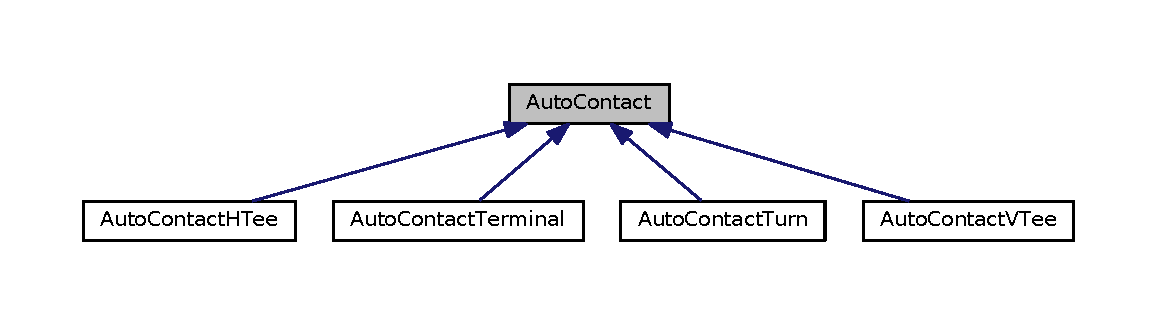
\includegraphics[width=350pt]{classKatabatic_1_1AutoContact__inherit__graph}
\end{center}
\end{figure}
\subsection*{Public Member Functions}
\begin{DoxyCompactItemize}
\item 
\textbf{ Hook} $\ast$ \mbox{\hyperlink{classKatabatic_1_1AutoContact_a4092778435abf3fb25a986a802bdb6c6}{get\+Body\+Hook}} ()
\item 
\textbf{ Hook} $\ast$ \mbox{\hyperlink{classKatabatic_1_1AutoContact_ad4a1ca46647528c32c5fbd4c45ac866c}{get\+Anchor\+Hook}} ()
\item 
\textbf{ Component} $\ast$ \mbox{\hyperlink{classKatabatic_1_1AutoContact_a142af2208e8c058c672bbad3640a6c46}{get\+Anchor}} () const
\item 
\textbf{ Net} $\ast$ \mbox{\hyperlink{classKatabatic_1_1AutoContact_a692492374623a5c6096b2c4a51190359}{get\+Net}} () const
\item 
const \textbf{ Layer} $\ast$ \mbox{\hyperlink{classKatabatic_1_1AutoContact_ab045567c4f529dca7790d66c17c3084f}{get\+Layer}} () const
\item 
\textbf{ Db\+U\+::\+Unit} \mbox{\hyperlink{classKatabatic_1_1AutoContact_a00b8f54c8171f6699e57de1b8c18eeb1}{getX}} () const
\item 
\textbf{ Db\+U\+::\+Unit} \mbox{\hyperlink{classKatabatic_1_1AutoContact_a4580de6b074712e400d5d238ce3af054}{getY}} () const
\item 
\textbf{ Db\+U\+::\+Unit} \mbox{\hyperlink{classKatabatic_1_1AutoContact_ad1ef5843ef3eabe27e548f24ca222876}{get\+Dx}} () const
\item 
\textbf{ Db\+U\+::\+Unit} \mbox{\hyperlink{classKatabatic_1_1AutoContact_ae4046e6ed80cbba54a48953ef4d2ca6d}{get\+Dy}} () const
\item 
\textbf{ Point} \mbox{\hyperlink{classKatabatic_1_1AutoContact_ac2ba7fbe2fad7d4910aa71ee034078e7}{get\+Center}} () const
\item 
\textbf{ Point} \mbox{\hyperlink{classKatabatic_1_1AutoContact_a4fa9bb12d79f6645884d567986c9b0a5}{get\+Position}} () const
\item 
\textbf{ Db\+U\+::\+Unit} \mbox{\hyperlink{classKatabatic_1_1AutoContact_a9c63fe7288748eaf5332ca796a36d872}{get\+Width}} () const
\item 
\textbf{ Db\+U\+::\+Unit} \mbox{\hyperlink{classKatabatic_1_1AutoContact_a5a345a7129c2a07f10f9f10c959616b9}{get\+Half\+Width}} () const
\item 
\textbf{ Db\+U\+::\+Unit} \mbox{\hyperlink{classKatabatic_1_1AutoContact_a3ade412549810d29d5ce3c860fc965b9}{get\+Height}} () const
\item 
\textbf{ Db\+U\+::\+Unit} \mbox{\hyperlink{classKatabatic_1_1AutoContact_a3ab7b800879862100636b003a5d168f3}{get\+Half\+Height}} () const
\item 
\textbf{ Components} \mbox{\hyperlink{classKatabatic_1_1AutoContact_ad59f45aaefd5acc8fb9795d4c0e49a7f}{get\+Slave\+Components}} () const
\item 
void \mbox{\hyperlink{classKatabatic_1_1AutoContact_aad4271c35e0162c8a4d034dca07f5a4b}{set\+Layer}} (const \textbf{ Layer} $\ast$)
\item 
void \mbox{\hyperlink{classKatabatic_1_1AutoContact_a9a0ec0a0ac85f23cfad6c069ea8dade7}{set\+Width}} (\textbf{ Db\+U\+::\+Unit})
\item 
void \mbox{\hyperlink{classKatabatic_1_1AutoContact_a106f372cee0916ebb6544627e47bb58d}{set\+Height}} (\textbf{ Db\+U\+::\+Unit})
\item 
void \mbox{\hyperlink{classKatabatic_1_1AutoContact_a0284fcec9bd41b26648e7bef3d4f1952}{set\+Sizes}} (\textbf{ Db\+U\+::\+Unit} width, \textbf{ Db\+U\+::\+Unit} height)
\item 
void \mbox{\hyperlink{classKatabatic_1_1AutoContact_a154f993d0262c92bfc0dc95154faf794}{setX}} (\textbf{ Db\+U\+::\+Unit})
\item 
void \mbox{\hyperlink{classKatabatic_1_1AutoContact_ac862ce450a533f0544d2168b132ba165}{setY}} (\textbf{ Db\+U\+::\+Unit})
\item 
void \mbox{\hyperlink{classKatabatic_1_1AutoContact_a12d3bfdce07580db21b17cf87f912cc3}{set\+Position}} (\textbf{ Db\+U\+::\+Unit} width, \textbf{ Db\+U\+::\+Unit} height)
\item 
void \mbox{\hyperlink{classKatabatic_1_1AutoContact_a52707afec84391e898e01c75b2713d32}{set\+Position}} (const \textbf{ Point} \&)
\item 
void \mbox{\hyperlink{classKatabatic_1_1AutoContact_a2c83ac6a03bbac090a8ab120d62c6e44}{set\+Dx}} (\textbf{ Db\+U\+::\+Unit})
\item 
void \mbox{\hyperlink{classKatabatic_1_1AutoContact_a123478e15e2544598851d0e907212841}{set\+Dy}} (\textbf{ Db\+U\+::\+Unit})
\item 
void \mbox{\hyperlink{classKatabatic_1_1AutoContact_a9881d5e969669b641c5de4f4d94e5d15}{set\+Offset}} (\textbf{ Db\+U\+::\+Unit} dx, \textbf{ Db\+U\+::\+Unit} dy)
\item 
virtual void \mbox{\hyperlink{classKatabatic_1_1AutoContact_a9161f1e2832e5e141a13863223322aa5}{translate}} (const \textbf{ Db\+U\+::\+Unit} \&tx, const \textbf{ Db\+U\+::\+Unit} \&ty)
\item 
bool \mbox{\hyperlink{classKatabatic_1_1AutoContact_a77e5036ce0c3628f5bf65e729ba875ba}{is\+In\+Creation\+Stage}} () const
\item 
bool \mbox{\hyperlink{classKatabatic_1_1AutoContact_ac540608485240ff88970131ebc02c1ab}{is\+Invalidated}} () const
\item 
bool \mbox{\hyperlink{classKatabatic_1_1AutoContact_a6d1120fc8800af5d269e72ce5c3ba629}{is\+Invalidated\+Cache}} () const
\item 
bool \mbox{\hyperlink{classKatabatic_1_1AutoContact_a249530ac086dbf92f981887cc633facf}{is\+Turn}} () const
\item 
bool \mbox{\hyperlink{classKatabatic_1_1AutoContact_ae4ba7bc2888f990818cbdb808260c47e}{is\+Tee}} (unsigned int direction) const
\item 
bool \mbox{\hyperlink{classKatabatic_1_1AutoContact_aeb66931d535cbd3d0f9bc525968e15f5}{is\+H\+Tee}} () const
\item 
bool \mbox{\hyperlink{classKatabatic_1_1AutoContact_ae38846b6213cccbc6f008b175b4604b0}{is\+V\+Tee}} () const
\item 
bool \mbox{\hyperlink{classKatabatic_1_1AutoContact_afd7362b850709bed8b61c1aa22399f97}{is\+Fixed}} () const
\item 
bool \mbox{\hyperlink{classKatabatic_1_1AutoContact_acc77b6de9050a86dc41e25888c8f81f6}{has\+Bad\+Topology}} () const
\item 
bool \mbox{\hyperlink{classKatabatic_1_1AutoContact_af783b79a1398450e28e2ea55c3eb8476}{can\+Destroy}} (unsigned int flags=0) const
\item 
bool \mbox{\hyperlink{classKatabatic_1_1AutoContact_a69d29e4d230a0111ca18e6e661a48f8b}{can\+Move\+Up}} (const \mbox{\hyperlink{classKatabatic_1_1AutoSegment}{Auto\+Segment}} $\ast$moved) const
\item 
\textbf{ Contact} $\ast$ \mbox{\hyperlink{classKatabatic_1_1AutoContact_ab422116c7edfacedd31711c96e3ec95b}{base}} () const
\item 
virtual const \textbf{ Name} \& \mbox{\hyperlink{classKatabatic_1_1AutoContact_a9e76ae5cee9320b65251387419c9432b}{get\+Name}} () const
\item 
size\+\_\+t \mbox{\hyperlink{classKatabatic_1_1AutoContact_a1e57c42301b9e58648863e7d5dc055e7}{get\+Id}} () const
\item 
virtual \textbf{ Box} \mbox{\hyperlink{classKatabatic_1_1AutoContact_ab5d8bf98ab5af6fcfebea1b9f446d5d7}{get\+Bounding\+Box}} () const
\item 
\mbox{\hyperlink{classKatabatic_1_1GCell}{G\+Cell}} $\ast$ \mbox{\hyperlink{classKatabatic_1_1AutoContact_a819cf639562a031a1e2e061fe1293d66}{get\+G\+Cell}} () const
\item 
virtual \mbox{\hyperlink{classKatabatic_1_1AutoSegment}{Auto\+Segment}} $\ast$ \mbox{\hyperlink{classKatabatic_1_1AutoContact_a48ab1d3bdf85712e4784ef83ef136939}{get\+Opposite}} (const \mbox{\hyperlink{classKatabatic_1_1AutoSegment}{Auto\+Segment}} $\ast$) const =0
\item 
virtual \mbox{\hyperlink{classKatabatic_1_1AutoSegment}{Auto\+Segment}} $\ast$ \mbox{\hyperlink{classKatabatic_1_1AutoContact_a994371005874f946cc0ac78005d38423}{get\+Perpandicular}} (const \mbox{\hyperlink{classKatabatic_1_1AutoSegment}{Auto\+Segment}} $\ast$) const =0
\item 
virtual \mbox{\hyperlink{classKatabatic_1_1AutoSegment}{Auto\+Segment}} $\ast$ \mbox{\hyperlink{classKatabatic_1_1AutoContact_a50531ded68cc5206fe104b8d8bf3bd87}{get\+Segment}} (unsigned int) const =0
\item 
unsigned int \mbox{\hyperlink{classKatabatic_1_1AutoContact_ada381cbb88211a7f63d30691b669b5e1}{get\+Min\+Depth}} () const
\item 
unsigned int \mbox{\hyperlink{classKatabatic_1_1AutoContact_ac350bb9d2d038287530fcf474987ba55}{get\+Max\+Depth}} () const
\item 
void \mbox{\hyperlink{classKatabatic_1_1AutoContact_ac607a624c0698056c5bccf405cf05ea7}{get\+Lengths}} (\textbf{ Db\+U\+::\+Unit} $\ast$lengths, Auto\+Segment\+::\+Depth\+Length\+Set \&)
\item 
virtual \textbf{ Box} \mbox{\hyperlink{classKatabatic_1_1AutoContact_a00ed934305dd186a284b7a13b5798cb6}{get\+Native\+Constraint\+Box}} () const
\item 
\textbf{ Interval} \mbox{\hyperlink{classKatabatic_1_1AutoContact_ab1fd3fec6dd56d40217b8a5ecacb1719}{get\+U\+Constraints}} (unsigned int direction) const
\item 
\textbf{ Db\+U\+::\+Unit} \mbox{\hyperlink{classKatabatic_1_1AutoContact_a347244bd3f3a59881a2dee9801c74618}{get\+C\+B\+X\+Min}} () const
\item 
\textbf{ Db\+U\+::\+Unit} \mbox{\hyperlink{classKatabatic_1_1AutoContact_a798750f964050c53c269a2e56d44b690}{get\+C\+B\+X\+Max}} () const
\item 
\textbf{ Db\+U\+::\+Unit} \mbox{\hyperlink{classKatabatic_1_1AutoContact_ad7ee1befb03ee85f237a36e2f5ab8e45}{get\+C\+B\+Y\+Min}} () const
\item 
\textbf{ Db\+U\+::\+Unit} \mbox{\hyperlink{classKatabatic_1_1AutoContact_a4e4061a17285b0c08c31cfee65947cb6}{get\+C\+B\+Y\+Max}} () const
\item 
\textbf{ Box} \mbox{\hyperlink{classKatabatic_1_1AutoContact_ae9d087a6cd3d459d7f4bea6bc8b08b49}{get\+Constraint\+Box}} () const
\item 
\textbf{ Box} \& \mbox{\hyperlink{classKatabatic_1_1AutoContact_ac2fe070a286356a24baa466b4fe5b74d}{intersect\+Constraint\+Box}} (\textbf{ Box} \&box) const
\item 
void \mbox{\hyperlink{classKatabatic_1_1AutoContact_aabac50fd9b8e1bba7289573973658d18}{invalidate}} (unsigned int flags=0)
\item 
virtual void \mbox{\hyperlink{classKatabatic_1_1AutoContact_af6a2454547eeb7f5a519970dcb467e90}{update\+Geometry}} ()=0
\item 
virtual void \mbox{\hyperlink{classKatabatic_1_1AutoContact_a690764ddc997fe9766a79c4b8e0c3e2f}{update\+Topology}} ()=0
\item 
void \mbox{\hyperlink{classKatabatic_1_1AutoContact_a66f92d8233776fb858075f78af451997}{show\+Topology\+Error}} (const std\+::string \&, unsigned int flags=0)
\item 
virtual void \mbox{\hyperlink{classKatabatic_1_1AutoContact_ac371cd5b837a8965c11297c197e70a45}{check\+Topology}} ()
\item 
void \mbox{\hyperlink{classKatabatic_1_1AutoContact_aa1a02e206437f1371a74cafc724b00d7}{set\+G\+Cell}} (\mbox{\hyperlink{classKatabatic_1_1GCell}{G\+Cell}} $\ast$)
\item 
void \mbox{\hyperlink{classKatabatic_1_1AutoContact_a9fcb986110e79bc0044f7bfe503acc0c}{set\+C\+B\+X\+Min}} (\textbf{ Db\+U\+::\+Unit} x\+Min)
\item 
void \mbox{\hyperlink{classKatabatic_1_1AutoContact_aaa7652f5db46cab9edb066d06ea979f9}{set\+C\+B\+X\+Max}} (\textbf{ Db\+U\+::\+Unit} x\+Max)
\item 
void \mbox{\hyperlink{classKatabatic_1_1AutoContact_a5b598929b39ad3ec202405b31ac02b1d}{set\+C\+B\+Y\+Min}} (\textbf{ Db\+U\+::\+Unit} y\+Min)
\item 
void \mbox{\hyperlink{classKatabatic_1_1AutoContact_a1fdb3737d910a966e150a86d885f3c05}{set\+C\+B\+Y\+Max}} (\textbf{ Db\+U\+::\+Unit} y\+Max)
\item 
void \mbox{\hyperlink{classKatabatic_1_1AutoContact_a5e5f791613d0ef8f4cf9e7d8f35dc4c5}{set\+Constraint\+Box}} (const \textbf{ Box} \&box)
\item 
bool \mbox{\hyperlink{classKatabatic_1_1AutoContact_ac893802d1c5518cab86f8341af817abe}{restrict\+Constraint\+Box}} (\textbf{ Db\+U\+::\+Unit} constraint\+Min, \textbf{ Db\+U\+::\+Unit} constraint\+Max, unsigned int flags=\mbox{\hyperlink{namespaceKatabatic_a2af2ad6b6441614038caf59d04b3b217aa5153b2cc25ebccca8616ce20ecd727a}{Kb\+Warn\+On\+Error}})
\item 
void \mbox{\hyperlink{classKatabatic_1_1AutoContact_a7fc4029992d75a62ce718e5e622f8ce9}{migrate\+Constraint\+Box}} (\mbox{\hyperlink{classKatabatic_1_1AutoContact}{Auto\+Contact}} $\ast$other)
\end{DoxyCompactItemize}
\subsection*{Static Public Member Functions}
\begin{DoxyCompactItemize}
\item 
static size\+\_\+t \mbox{\hyperlink{classKatabatic_1_1AutoContact_a91c8bc1a6bdb1b15c3c084ebfd38af47}{get\+Allocateds}} ()
\item 
static const \textbf{ Name} \& \mbox{\hyperlink{classKatabatic_1_1AutoContact_a00e56270cfb31f56e52e31afbc33ba71}{get\+Static\+Name}} ()
\end{DoxyCompactItemize}
\subsection*{Static Protected Member Functions}
\begin{DoxyCompactItemize}
\item 
static void \mbox{\hyperlink{classKatabatic_1_1AutoContact_a2294ddd6bd4bda59c3453cc4dbd4f4fa}{\+\_\+get\+Topology}} (\textbf{ Contact} $\ast$, \textbf{ Component} $\ast$\&anchor, \textbf{ Horizontal} $\ast$$\ast$\&, \textbf{ Vertical} $\ast$$\ast$\&, size\+\_\+t)
\end{DoxyCompactItemize}


\subsection{Detailed Description}
Abstract base class for \mbox{\hyperlink{classKatabatic_1_1AutoContact}{Auto\+Contact}}. 

\hypertarget{classKatabatic_1_1AutoContact_secACCache}{}\subsection{Caching Mechanism}\label{classKatabatic_1_1AutoContact_secACCache}
To bypass the Ring/\+Hook mechanism {\itshape and} the subsequent Session\+::\+Lookup() call, the Auto\+Segments anchored on an \mbox{\hyperlink{classKatabatic_1_1AutoContact}{Auto\+Contact}} are cached in the \mbox{\hyperlink{classKatabatic_1_1AutoContact}{Auto\+Contact}} itself. They can be accessed through {\ttfamily get\+Horizontal\+N()} and get\+Vertical\+N() accessors {\ttfamily N} depending on the subtype of \mbox{\hyperlink{classKatabatic_1_1AutoContact}{Auto\+Contact}}.

Cached Auto\+Segments are updated in the \mbox{\hyperlink{classKatabatic_1_1AutoContact_a690764ddc997fe9766a79c4b8e0c3e2f}{Auto\+Contact\+::update\+Topology()}} function only.\hypertarget{classKatabatic_1_1AutoContact_secACInvalidate}{}\subsection{Invalidate on Auto\+Contacts}\label{classKatabatic_1_1AutoContact_secACInvalidate}
The invalidation of an \mbox{\hyperlink{classKatabatic_1_1AutoContact}{Auto\+Contact}} invalidate all the segments that are anchored on it.

{\bfseries Special Case of H\+Tee \& V\+Tee}

When invalidating an H\+Tee or V\+Tee, two out of the three anchored segments are parallels. The {\itshape aligned} constraint is passed on those two. By default, when we invalidate an \mbox{\hyperlink{classKatabatic_1_1AutoSegment}{Auto\+Segment}}, the invalidation is applied to the whole aligned set through the \mbox{\hyperlink{classKatabatic_1_1AutoSegment_aaca749f49cd03ca06449d5ea2104033a}{Auto\+Segment\+::get\+Aligneds()}} collection. So if one of the parallel is invalidated and the other not, it should only be because we are already in {\ttfamily get\+Aligneds()}, then we do not want to invalidate again the whole aligned set. In that case, we perform an atomic only invalidation (reset \mbox{\hyperlink{namespaceKatabatic_a2af2ad6b6441614038caf59d04b3b217a3f95c1f06fe0b58b44ccbc57d99f2a5d}{Katabatic\+::\+Kb\+Propagate}}).

For the complete invalidation/revalidation mechanism see \mbox{\hyperlink{classKatabatic_1_1Session_secSessionAlgo}{Session Algorithm}}.\hypertarget{classKatabatic_1_1AutoContact_secDiffFromKatabatic2}{}\subsection{Notes -\/ Differences from Katabatic 2}\label{classKatabatic_1_1AutoContact_secDiffFromKatabatic2}
From the previous version of \mbox{\hyperlink{namespaceKatabatic}{Katabatic}}, \mbox{\hyperlink{classKatabatic_1_1AutoContact}{Auto\+Contact}} have been greatly stripped down (again). They are now always punctual objetcs with stricly fixed topologies\+: 
\begin{DoxyItemize}
\item \mbox{\hyperlink{classKatabatic_1_1AutoContactTerminal}{Auto\+Contact\+Terminal}} to connect to a terminal (one segment). 
\item \mbox{\hyperlink{classKatabatic_1_1AutoContactTurn}{Auto\+Contact\+Turn}} to make a turn\+: two perpandiculars segments. 
\item \mbox{\hyperlink{classKatabatic_1_1AutoContactHTee}{Auto\+Contact\+H\+Tee}} an horizontal tee\+: two {\itshape aligned} horizonals and one vertical. 
\item \mbox{\hyperlink{classKatabatic_1_1AutoContactVTee}{Auto\+Contact\+V\+Tee}} an horizontal tee\+: two {\itshape aligned} verticals and one horizontal. 
\end{DoxyItemize}

\subsection{Member Function Documentation}
\mbox{\Hypertarget{classKatabatic_1_1AutoContact_a4092778435abf3fb25a986a802bdb6c6}\label{classKatabatic_1_1AutoContact_a4092778435abf3fb25a986a802bdb6c6}} 
\index{Katabatic\+::\+Auto\+Contact@{Katabatic\+::\+Auto\+Contact}!get\+Body\+Hook@{get\+Body\+Hook}}
\index{get\+Body\+Hook@{get\+Body\+Hook}!Katabatic\+::\+Auto\+Contact@{Katabatic\+::\+Auto\+Contact}}
\subsubsection{\texorpdfstring{get\+Body\+Hook()}{getBodyHook()}}
{\footnotesize\ttfamily \textbf{ Hook} $\ast$ get\+Body\+Hook (\begin{DoxyParamCaption}{ }\end{DoxyParamCaption})\hspace{0.3cm}{\ttfamily [inline]}}

{\itshape Base class method proxy.} 

References Component\+::get\+Body\+Hook().



Referenced by G\+Cell\+Topology\+::\+\_\+do\+\_\+x\+G\+\_\+1\+Pad(), and Auto\+Segment\+::create().

\mbox{\Hypertarget{classKatabatic_1_1AutoContact_ad4a1ca46647528c32c5fbd4c45ac866c}\label{classKatabatic_1_1AutoContact_ad4a1ca46647528c32c5fbd4c45ac866c}} 
\index{Katabatic\+::\+Auto\+Contact@{Katabatic\+::\+Auto\+Contact}!get\+Anchor\+Hook@{get\+Anchor\+Hook}}
\index{get\+Anchor\+Hook@{get\+Anchor\+Hook}!Katabatic\+::\+Auto\+Contact@{Katabatic\+::\+Auto\+Contact}}
\subsubsection{\texorpdfstring{get\+Anchor\+Hook()}{getAnchorHook()}}
{\footnotesize\ttfamily \textbf{ Hook} $\ast$ get\+Anchor\+Hook (\begin{DoxyParamCaption}{ }\end{DoxyParamCaption})\hspace{0.3cm}{\ttfamily [inline]}}

{\itshape Base class method proxy.} 

References Contact\+::get\+Anchor\+Hook().

\mbox{\Hypertarget{classKatabatic_1_1AutoContact_a142af2208e8c058c672bbad3640a6c46}\label{classKatabatic_1_1AutoContact_a142af2208e8c058c672bbad3640a6c46}} 
\index{Katabatic\+::\+Auto\+Contact@{Katabatic\+::\+Auto\+Contact}!get\+Anchor@{get\+Anchor}}
\index{get\+Anchor@{get\+Anchor}!Katabatic\+::\+Auto\+Contact@{Katabatic\+::\+Auto\+Contact}}
\subsubsection{\texorpdfstring{get\+Anchor()}{getAnchor()}}
{\footnotesize\ttfamily \textbf{ Component} $\ast$ get\+Anchor (\begin{DoxyParamCaption}{ }\end{DoxyParamCaption}) const\hspace{0.3cm}{\ttfamily [inline]}}

{\itshape Base class method proxy.} 

References Contact\+::get\+Anchor().



Referenced by Auto\+Contact\+Terminal\+::get\+Native\+Constraint\+Box(), and Auto\+Contact\+Terminal\+::update\+Topology().

\mbox{\Hypertarget{classKatabatic_1_1AutoContact_a692492374623a5c6096b2c4a51190359}\label{classKatabatic_1_1AutoContact_a692492374623a5c6096b2c4a51190359}} 
\index{Katabatic\+::\+Auto\+Contact@{Katabatic\+::\+Auto\+Contact}!get\+Net@{get\+Net}}
\index{get\+Net@{get\+Net}!Katabatic\+::\+Auto\+Contact@{Katabatic\+::\+Auto\+Contact}}
\subsubsection{\texorpdfstring{get\+Net()}{getNet()}}
{\footnotesize\ttfamily \textbf{ Net} $\ast$ get\+Net (\begin{DoxyParamCaption}{ }\end{DoxyParamCaption}) const\hspace{0.3cm}{\ttfamily [inline]}}

{\itshape Base class method proxy.} 

References Component\+::get\+Net().



Referenced by Auto\+Contact\+V\+Tee\+::update\+Geometry(), Auto\+Contact\+Turn\+::update\+Geometry(), Auto\+Contact\+H\+Tee\+::update\+Geometry(), Auto\+Contact\+Terminal\+::update\+Geometry(), Auto\+Contact\+V\+Tee\+::update\+Topology(), Auto\+Contact\+Turn\+::update\+Topology(), Auto\+Contact\+H\+Tee\+::update\+Topology(), and Auto\+Contact\+Terminal\+::update\+Topology().

\mbox{\Hypertarget{classKatabatic_1_1AutoContact_ab045567c4f529dca7790d66c17c3084f}\label{classKatabatic_1_1AutoContact_ab045567c4f529dca7790d66c17c3084f}} 
\index{Katabatic\+::\+Auto\+Contact@{Katabatic\+::\+Auto\+Contact}!get\+Layer@{get\+Layer}}
\index{get\+Layer@{get\+Layer}!Katabatic\+::\+Auto\+Contact@{Katabatic\+::\+Auto\+Contact}}
\subsubsection{\texorpdfstring{get\+Layer()}{getLayer()}}
{\footnotesize\ttfamily const \textbf{ Layer} $\ast$ get\+Layer (\begin{DoxyParamCaption}{ }\end{DoxyParamCaption}) const\hspace{0.3cm}{\ttfamily [inline]}}

{\itshape Base class method proxy.} 

References Component\+::get\+Layer().



Referenced by Auto\+Segment\+::make\+Dogleg(), Auto\+Segment\+::revalidate(), Auto\+Contact\+V\+Tee\+::update\+Topology(), Auto\+Contact\+Turn\+::update\+Topology(), Auto\+Contact\+H\+Tee\+::update\+Topology(), and Auto\+Contact\+Terminal\+::update\+Topology().

\mbox{\Hypertarget{classKatabatic_1_1AutoContact_a00b8f54c8171f6699e57de1b8c18eeb1}\label{classKatabatic_1_1AutoContact_a00b8f54c8171f6699e57de1b8c18eeb1}} 
\index{Katabatic\+::\+Auto\+Contact@{Katabatic\+::\+Auto\+Contact}!getX@{getX}}
\index{getX@{getX}!Katabatic\+::\+Auto\+Contact@{Katabatic\+::\+Auto\+Contact}}
\subsubsection{\texorpdfstring{get\+X()}{getX()}}
{\footnotesize\ttfamily \textbf{ Db\+U\+::\+Unit} getX (\begin{DoxyParamCaption}{ }\end{DoxyParamCaption}) const\hspace{0.3cm}{\ttfamily [inline]}}

{\itshape Base class method proxy.} 

References Component\+::get\+X().



Referenced by G\+Cell\+Topology\+::\+\_\+do\+\_\+1\+G\+\_\+1\+M3(), G\+Cell\+Topology\+::\+\_\+do\+\_\+x\+G\+\_\+x\+M3(), Auto\+Segment\+::create(), G\+Cell\+Topology\+::do\+Rp\+\_\+\+Stair\+Case\+V(), Auto\+Segment\+::make\+Dogleg(), Auto\+Contact\+V\+Tee\+::update\+Geometry(), Auto\+Contact\+Turn\+::update\+Geometry(), and Auto\+Contact\+H\+Tee\+::update\+Geometry().

\mbox{\Hypertarget{classKatabatic_1_1AutoContact_a4580de6b074712e400d5d238ce3af054}\label{classKatabatic_1_1AutoContact_a4580de6b074712e400d5d238ce3af054}} 
\index{Katabatic\+::\+Auto\+Contact@{Katabatic\+::\+Auto\+Contact}!getY@{getY}}
\index{getY@{getY}!Katabatic\+::\+Auto\+Contact@{Katabatic\+::\+Auto\+Contact}}
\subsubsection{\texorpdfstring{get\+Y()}{getY()}}
{\footnotesize\ttfamily \textbf{ Db\+U\+::\+Unit} getY (\begin{DoxyParamCaption}{ }\end{DoxyParamCaption}) const\hspace{0.3cm}{\ttfamily [inline]}}

{\itshape Base class method proxy.} 

References Component\+::get\+Y().



Referenced by Auto\+Segment\+::create(), G\+Cell\+Topology\+::do\+Rp\+\_\+\+Stair\+Case\+H(), Auto\+Segment\+::make\+Dogleg(), Auto\+Contact\+V\+Tee\+::update\+Geometry(), Auto\+Contact\+Turn\+::update\+Geometry(), and Auto\+Contact\+H\+Tee\+::update\+Geometry().

\mbox{\Hypertarget{classKatabatic_1_1AutoContact_ad1ef5843ef3eabe27e548f24ca222876}\label{classKatabatic_1_1AutoContact_ad1ef5843ef3eabe27e548f24ca222876}} 
\index{Katabatic\+::\+Auto\+Contact@{Katabatic\+::\+Auto\+Contact}!get\+Dx@{get\+Dx}}
\index{get\+Dx@{get\+Dx}!Katabatic\+::\+Auto\+Contact@{Katabatic\+::\+Auto\+Contact}}
\subsubsection{\texorpdfstring{get\+Dx()}{getDx()}}
{\footnotesize\ttfamily \textbf{ Db\+U\+::\+Unit} get\+Dx (\begin{DoxyParamCaption}{ }\end{DoxyParamCaption}) const\hspace{0.3cm}{\ttfamily [inline]}}

{\itshape Base class method proxy.} 

References Contact\+::get\+Dx().

\mbox{\Hypertarget{classKatabatic_1_1AutoContact_ae4046e6ed80cbba54a48953ef4d2ca6d}\label{classKatabatic_1_1AutoContact_ae4046e6ed80cbba54a48953ef4d2ca6d}} 
\index{Katabatic\+::\+Auto\+Contact@{Katabatic\+::\+Auto\+Contact}!get\+Dy@{get\+Dy}}
\index{get\+Dy@{get\+Dy}!Katabatic\+::\+Auto\+Contact@{Katabatic\+::\+Auto\+Contact}}
\subsubsection{\texorpdfstring{get\+Dy()}{getDy()}}
{\footnotesize\ttfamily \textbf{ Db\+U\+::\+Unit} get\+Dy (\begin{DoxyParamCaption}{ }\end{DoxyParamCaption}) const\hspace{0.3cm}{\ttfamily [inline]}}

{\itshape Base class method proxy.} 

References Contact\+::get\+Dy().

\mbox{\Hypertarget{classKatabatic_1_1AutoContact_ac2ba7fbe2fad7d4910aa71ee034078e7}\label{classKatabatic_1_1AutoContact_ac2ba7fbe2fad7d4910aa71ee034078e7}} 
\index{Katabatic\+::\+Auto\+Contact@{Katabatic\+::\+Auto\+Contact}!get\+Center@{get\+Center}}
\index{get\+Center@{get\+Center}!Katabatic\+::\+Auto\+Contact@{Katabatic\+::\+Auto\+Contact}}
\subsubsection{\texorpdfstring{get\+Center()}{getCenter()}}
{\footnotesize\ttfamily \textbf{ Point} get\+Center (\begin{DoxyParamCaption}{ }\end{DoxyParamCaption}) const\hspace{0.3cm}{\ttfamily [inline]}}

{\itshape Base class method proxy.} \mbox{\Hypertarget{classKatabatic_1_1AutoContact_a4fa9bb12d79f6645884d567986c9b0a5}\label{classKatabatic_1_1AutoContact_a4fa9bb12d79f6645884d567986c9b0a5}} 
\index{Katabatic\+::\+Auto\+Contact@{Katabatic\+::\+Auto\+Contact}!get\+Position@{get\+Position}}
\index{get\+Position@{get\+Position}!Katabatic\+::\+Auto\+Contact@{Katabatic\+::\+Auto\+Contact}}
\subsubsection{\texorpdfstring{get\+Position()}{getPosition()}}
{\footnotesize\ttfamily \textbf{ Point} get\+Position (\begin{DoxyParamCaption}{ }\end{DoxyParamCaption}) const\hspace{0.3cm}{\ttfamily [inline]}}

{\itshape Base class method proxy.} 

References Component\+::get\+Position().

\mbox{\Hypertarget{classKatabatic_1_1AutoContact_a9c63fe7288748eaf5332ca796a36d872}\label{classKatabatic_1_1AutoContact_a9c63fe7288748eaf5332ca796a36d872}} 
\index{Katabatic\+::\+Auto\+Contact@{Katabatic\+::\+Auto\+Contact}!get\+Width@{get\+Width}}
\index{get\+Width@{get\+Width}!Katabatic\+::\+Auto\+Contact@{Katabatic\+::\+Auto\+Contact}}
\subsubsection{\texorpdfstring{get\+Width()}{getWidth()}}
{\footnotesize\ttfamily \textbf{ Db\+U\+::\+Unit} get\+Width (\begin{DoxyParamCaption}{ }\end{DoxyParamCaption}) const\hspace{0.3cm}{\ttfamily [inline]}}

{\itshape Base class method proxy.} 

References Contact\+::get\+Width().

\mbox{\Hypertarget{classKatabatic_1_1AutoContact_a5a345a7129c2a07f10f9f10c959616b9}\label{classKatabatic_1_1AutoContact_a5a345a7129c2a07f10f9f10c959616b9}} 
\index{Katabatic\+::\+Auto\+Contact@{Katabatic\+::\+Auto\+Contact}!get\+Half\+Width@{get\+Half\+Width}}
\index{get\+Half\+Width@{get\+Half\+Width}!Katabatic\+::\+Auto\+Contact@{Katabatic\+::\+Auto\+Contact}}
\subsubsection{\texorpdfstring{get\+Half\+Width()}{getHalfWidth()}}
{\footnotesize\ttfamily \textbf{ Db\+U\+::\+Unit} get\+Half\+Width (\begin{DoxyParamCaption}{ }\end{DoxyParamCaption}) const\hspace{0.3cm}{\ttfamily [inline]}}

{\itshape Base class method proxy.} 

References Contact\+::get\+Half\+Width().

\mbox{\Hypertarget{classKatabatic_1_1AutoContact_a3ade412549810d29d5ce3c860fc965b9}\label{classKatabatic_1_1AutoContact_a3ade412549810d29d5ce3c860fc965b9}} 
\index{Katabatic\+::\+Auto\+Contact@{Katabatic\+::\+Auto\+Contact}!get\+Height@{get\+Height}}
\index{get\+Height@{get\+Height}!Katabatic\+::\+Auto\+Contact@{Katabatic\+::\+Auto\+Contact}}
\subsubsection{\texorpdfstring{get\+Height()}{getHeight()}}
{\footnotesize\ttfamily \textbf{ Db\+U\+::\+Unit} get\+Height (\begin{DoxyParamCaption}{ }\end{DoxyParamCaption}) const\hspace{0.3cm}{\ttfamily [inline]}}

{\itshape Base class method proxy.} 

References Contact\+::get\+Height().

\mbox{\Hypertarget{classKatabatic_1_1AutoContact_a3ab7b800879862100636b003a5d168f3}\label{classKatabatic_1_1AutoContact_a3ab7b800879862100636b003a5d168f3}} 
\index{Katabatic\+::\+Auto\+Contact@{Katabatic\+::\+Auto\+Contact}!get\+Half\+Height@{get\+Half\+Height}}
\index{get\+Half\+Height@{get\+Half\+Height}!Katabatic\+::\+Auto\+Contact@{Katabatic\+::\+Auto\+Contact}}
\subsubsection{\texorpdfstring{get\+Half\+Height()}{getHalfHeight()}}
{\footnotesize\ttfamily \textbf{ Db\+U\+::\+Unit} get\+Half\+Height (\begin{DoxyParamCaption}{ }\end{DoxyParamCaption}) const\hspace{0.3cm}{\ttfamily [inline]}}

{\itshape Base class method proxy.} 

References Contact\+::get\+Half\+Height().

\mbox{\Hypertarget{classKatabatic_1_1AutoContact_ad59f45aaefd5acc8fb9795d4c0e49a7f}\label{classKatabatic_1_1AutoContact_ad59f45aaefd5acc8fb9795d4c0e49a7f}} 
\index{Katabatic\+::\+Auto\+Contact@{Katabatic\+::\+Auto\+Contact}!get\+Slave\+Components@{get\+Slave\+Components}}
\index{get\+Slave\+Components@{get\+Slave\+Components}!Katabatic\+::\+Auto\+Contact@{Katabatic\+::\+Auto\+Contact}}
\subsubsection{\texorpdfstring{get\+Slave\+Components()}{getSlaveComponents()}}
{\footnotesize\ttfamily \textbf{ Components} get\+Slave\+Components (\begin{DoxyParamCaption}{ }\end{DoxyParamCaption}) const\hspace{0.3cm}{\ttfamily [inline]}}

{\itshape Base class method proxy.} 

References Component\+::get\+Slave\+Components().

\mbox{\Hypertarget{classKatabatic_1_1AutoContact_aad4271c35e0162c8a4d034dca07f5a4b}\label{classKatabatic_1_1AutoContact_aad4271c35e0162c8a4d034dca07f5a4b}} 
\index{Katabatic\+::\+Auto\+Contact@{Katabatic\+::\+Auto\+Contact}!set\+Layer@{set\+Layer}}
\index{set\+Layer@{set\+Layer}!Katabatic\+::\+Auto\+Contact@{Katabatic\+::\+Auto\+Contact}}
\subsubsection{\texorpdfstring{set\+Layer()}{setLayer()}}
{\footnotesize\ttfamily void set\+Layer (\begin{DoxyParamCaption}\item[{const \textbf{ Layer} $\ast$}]{layer }\end{DoxyParamCaption})\hspace{0.3cm}{\ttfamily [inline]}}

{\itshape Base class method proxy.} 

References Contact\+::set\+Layer().



Referenced by Auto\+Segment\+::reduce\+Dogleg\+Layer(), Auto\+Contact\+V\+Tee\+::update\+Topology(), Auto\+Contact\+Turn\+::update\+Topology(), Auto\+Contact\+H\+Tee\+::update\+Topology(), and Auto\+Contact\+Terminal\+::update\+Topology().

\mbox{\Hypertarget{classKatabatic_1_1AutoContact_a9a0ec0a0ac85f23cfad6c069ea8dade7}\label{classKatabatic_1_1AutoContact_a9a0ec0a0ac85f23cfad6c069ea8dade7}} 
\index{Katabatic\+::\+Auto\+Contact@{Katabatic\+::\+Auto\+Contact}!set\+Width@{set\+Width}}
\index{set\+Width@{set\+Width}!Katabatic\+::\+Auto\+Contact@{Katabatic\+::\+Auto\+Contact}}
\subsubsection{\texorpdfstring{set\+Width()}{setWidth()}}
{\footnotesize\ttfamily void set\+Width (\begin{DoxyParamCaption}\item[{\textbf{ Db\+U\+::\+Unit}}]{w }\end{DoxyParamCaption})\hspace{0.3cm}{\ttfamily [inline]}}

{\itshape Base class method proxy.} 

References Contact\+::set\+Width().

\mbox{\Hypertarget{classKatabatic_1_1AutoContact_a106f372cee0916ebb6544627e47bb58d}\label{classKatabatic_1_1AutoContact_a106f372cee0916ebb6544627e47bb58d}} 
\index{Katabatic\+::\+Auto\+Contact@{Katabatic\+::\+Auto\+Contact}!set\+Height@{set\+Height}}
\index{set\+Height@{set\+Height}!Katabatic\+::\+Auto\+Contact@{Katabatic\+::\+Auto\+Contact}}
\subsubsection{\texorpdfstring{set\+Height()}{setHeight()}}
{\footnotesize\ttfamily void set\+Height (\begin{DoxyParamCaption}\item[{\textbf{ Db\+U\+::\+Unit}}]{h }\end{DoxyParamCaption})\hspace{0.3cm}{\ttfamily [inline]}}

{\itshape Base class method proxy.} 

References Contact\+::set\+Height().

\mbox{\Hypertarget{classKatabatic_1_1AutoContact_a0284fcec9bd41b26648e7bef3d4f1952}\label{classKatabatic_1_1AutoContact_a0284fcec9bd41b26648e7bef3d4f1952}} 
\index{Katabatic\+::\+Auto\+Contact@{Katabatic\+::\+Auto\+Contact}!set\+Sizes@{set\+Sizes}}
\index{set\+Sizes@{set\+Sizes}!Katabatic\+::\+Auto\+Contact@{Katabatic\+::\+Auto\+Contact}}
\subsubsection{\texorpdfstring{set\+Sizes()}{setSizes()}}
{\footnotesize\ttfamily void set\+Sizes (\begin{DoxyParamCaption}\item[{\textbf{ Db\+U\+::\+Unit}}]{w,  }\item[{\textbf{ Db\+U\+::\+Unit}}]{h }\end{DoxyParamCaption})\hspace{0.3cm}{\ttfamily [inline]}}

{\itshape Base class method proxy.} 

References Contact\+::set\+Sizes().

\mbox{\Hypertarget{classKatabatic_1_1AutoContact_a154f993d0262c92bfc0dc95154faf794}\label{classKatabatic_1_1AutoContact_a154f993d0262c92bfc0dc95154faf794}} 
\index{Katabatic\+::\+Auto\+Contact@{Katabatic\+::\+Auto\+Contact}!setX@{setX}}
\index{setX@{setX}!Katabatic\+::\+Auto\+Contact@{Katabatic\+::\+Auto\+Contact}}
\subsubsection{\texorpdfstring{set\+X()}{setX()}}
{\footnotesize\ttfamily void setX (\begin{DoxyParamCaption}\item[{\textbf{ Db\+U\+::\+Unit}}]{x }\end{DoxyParamCaption})\hspace{0.3cm}{\ttfamily [inline]}}

{\itshape Base class method proxy.} 

References Contact\+::set\+X().



Referenced by Auto\+Vertical\+::\+\_\+post\+Create(), Auto\+Contact\+V\+Tee\+::update\+Geometry(), Auto\+Contact\+Turn\+::update\+Geometry(), Auto\+Contact\+H\+Tee\+::update\+Geometry(), and Auto\+Contact\+Terminal\+::update\+Geometry().

\mbox{\Hypertarget{classKatabatic_1_1AutoContact_ac862ce450a533f0544d2168b132ba165}\label{classKatabatic_1_1AutoContact_ac862ce450a533f0544d2168b132ba165}} 
\index{Katabatic\+::\+Auto\+Contact@{Katabatic\+::\+Auto\+Contact}!setY@{setY}}
\index{setY@{setY}!Katabatic\+::\+Auto\+Contact@{Katabatic\+::\+Auto\+Contact}}
\subsubsection{\texorpdfstring{set\+Y()}{setY()}}
{\footnotesize\ttfamily void setY (\begin{DoxyParamCaption}\item[{\textbf{ Db\+U\+::\+Unit}}]{y }\end{DoxyParamCaption})\hspace{0.3cm}{\ttfamily [inline]}}

{\itshape Base class method proxy.} 

References Contact\+::set\+Y().



Referenced by Auto\+Horizontal\+::\+\_\+post\+Create(), Auto\+Contact\+V\+Tee\+::update\+Geometry(), Auto\+Contact\+Turn\+::update\+Geometry(), Auto\+Contact\+H\+Tee\+::update\+Geometry(), and Auto\+Contact\+Terminal\+::update\+Geometry().

\mbox{\Hypertarget{classKatabatic_1_1AutoContact_a12d3bfdce07580db21b17cf87f912cc3}\label{classKatabatic_1_1AutoContact_a12d3bfdce07580db21b17cf87f912cc3}} 
\index{Katabatic\+::\+Auto\+Contact@{Katabatic\+::\+Auto\+Contact}!set\+Position@{set\+Position}}
\index{set\+Position@{set\+Position}!Katabatic\+::\+Auto\+Contact@{Katabatic\+::\+Auto\+Contact}}
\subsubsection{\texorpdfstring{set\+Position()}{setPosition()}\hspace{0.1cm}{\footnotesize\ttfamily [1/2]}}
{\footnotesize\ttfamily void set\+Position (\begin{DoxyParamCaption}\item[{\textbf{ Db\+U\+::\+Unit}}]{w,  }\item[{\textbf{ Db\+U\+::\+Unit}}]{h }\end{DoxyParamCaption})\hspace{0.3cm}{\ttfamily [inline]}}

{\itshape Base class method proxy.} 

References Contact\+::set\+Position().

\mbox{\Hypertarget{classKatabatic_1_1AutoContact_a52707afec84391e898e01c75b2713d32}\label{classKatabatic_1_1AutoContact_a52707afec84391e898e01c75b2713d32}} 
\index{Katabatic\+::\+Auto\+Contact@{Katabatic\+::\+Auto\+Contact}!set\+Position@{set\+Position}}
\index{set\+Position@{set\+Position}!Katabatic\+::\+Auto\+Contact@{Katabatic\+::\+Auto\+Contact}}
\subsubsection{\texorpdfstring{set\+Position()}{setPosition()}\hspace{0.1cm}{\footnotesize\ttfamily [2/2]}}
{\footnotesize\ttfamily void set\+Position (\begin{DoxyParamCaption}\item[{const \textbf{ Point} \&}]{p }\end{DoxyParamCaption})\hspace{0.3cm}{\ttfamily [inline]}}

{\itshape Base class method proxy.} 

References Contact\+::set\+Position().

\mbox{\Hypertarget{classKatabatic_1_1AutoContact_a2c83ac6a03bbac090a8ab120d62c6e44}\label{classKatabatic_1_1AutoContact_a2c83ac6a03bbac090a8ab120d62c6e44}} 
\index{Katabatic\+::\+Auto\+Contact@{Katabatic\+::\+Auto\+Contact}!set\+Dx@{set\+Dx}}
\index{set\+Dx@{set\+Dx}!Katabatic\+::\+Auto\+Contact@{Katabatic\+::\+Auto\+Contact}}
\subsubsection{\texorpdfstring{set\+Dx()}{setDx()}}
{\footnotesize\ttfamily void set\+Dx (\begin{DoxyParamCaption}\item[{\textbf{ Db\+U\+::\+Unit}}]{dx }\end{DoxyParamCaption})\hspace{0.3cm}{\ttfamily [inline]}}

{\itshape Base class method proxy.} 

References Contact\+::set\+Dx().

\mbox{\Hypertarget{classKatabatic_1_1AutoContact_a123478e15e2544598851d0e907212841}\label{classKatabatic_1_1AutoContact_a123478e15e2544598851d0e907212841}} 
\index{Katabatic\+::\+Auto\+Contact@{Katabatic\+::\+Auto\+Contact}!set\+Dy@{set\+Dy}}
\index{set\+Dy@{set\+Dy}!Katabatic\+::\+Auto\+Contact@{Katabatic\+::\+Auto\+Contact}}
\subsubsection{\texorpdfstring{set\+Dy()}{setDy()}}
{\footnotesize\ttfamily void set\+Dy (\begin{DoxyParamCaption}\item[{\textbf{ Db\+U\+::\+Unit}}]{dy }\end{DoxyParamCaption})\hspace{0.3cm}{\ttfamily [inline]}}

{\itshape Base class method proxy.} 

References Contact\+::set\+Dy().

\mbox{\Hypertarget{classKatabatic_1_1AutoContact_a9881d5e969669b641c5de4f4d94e5d15}\label{classKatabatic_1_1AutoContact_a9881d5e969669b641c5de4f4d94e5d15}} 
\index{Katabatic\+::\+Auto\+Contact@{Katabatic\+::\+Auto\+Contact}!set\+Offset@{set\+Offset}}
\index{set\+Offset@{set\+Offset}!Katabatic\+::\+Auto\+Contact@{Katabatic\+::\+Auto\+Contact}}
\subsubsection{\texorpdfstring{set\+Offset()}{setOffset()}}
{\footnotesize\ttfamily void set\+Offset (\begin{DoxyParamCaption}\item[{\textbf{ Db\+U\+::\+Unit}}]{w,  }\item[{\textbf{ Db\+U\+::\+Unit}}]{h }\end{DoxyParamCaption})\hspace{0.3cm}{\ttfamily [inline]}}

{\itshape Base class method proxy.} 

References Contact\+::set\+Offset().

\mbox{\Hypertarget{classKatabatic_1_1AutoContact_a9161f1e2832e5e141a13863223322aa5}\label{classKatabatic_1_1AutoContact_a9161f1e2832e5e141a13863223322aa5}} 
\index{Katabatic\+::\+Auto\+Contact@{Katabatic\+::\+Auto\+Contact}!translate@{translate}}
\index{translate@{translate}!Katabatic\+::\+Auto\+Contact@{Katabatic\+::\+Auto\+Contact}}
\subsubsection{\texorpdfstring{translate()}{translate()}}
{\footnotesize\ttfamily void translate (\begin{DoxyParamCaption}\item[{const \textbf{ Db\+U\+::\+Unit} \&}]{dx,  }\item[{const \textbf{ Db\+U\+::\+Unit} \&}]{dy }\end{DoxyParamCaption})\hspace{0.3cm}{\ttfamily [virtual]}}

{\itshape Base class method proxy.} \mbox{\Hypertarget{classKatabatic_1_1AutoContact_a77e5036ce0c3628f5bf65e729ba875ba}\label{classKatabatic_1_1AutoContact_a77e5036ce0c3628f5bf65e729ba875ba}} 
\index{Katabatic\+::\+Auto\+Contact@{Katabatic\+::\+Auto\+Contact}!is\+In\+Creation\+Stage@{is\+In\+Creation\+Stage}}
\index{is\+In\+Creation\+Stage@{is\+In\+Creation\+Stage}!Katabatic\+::\+Auto\+Contact@{Katabatic\+::\+Auto\+Contact}}
\subsubsection{\texorpdfstring{is\+In\+Creation\+Stage()}{isInCreationStage()}}
{\footnotesize\ttfamily bool is\+In\+Creation\+Stage (\begin{DoxyParamCaption}{ }\end{DoxyParamCaption}) const\hspace{0.3cm}{\ttfamily [inline]}}

{\bfseries Returns\+:} {\bfseries true} if the \mbox{\hyperlink{classKatabatic_1_1AutoContact}{Auto\+Contact}} is still in it\textquotesingle{}s initial creation stage. 

References Katabatic\+::\+Cnt\+In\+Creation\+Stage.

\mbox{\Hypertarget{classKatabatic_1_1AutoContact_ac540608485240ff88970131ebc02c1ab}\label{classKatabatic_1_1AutoContact_ac540608485240ff88970131ebc02c1ab}} 
\index{Katabatic\+::\+Auto\+Contact@{Katabatic\+::\+Auto\+Contact}!is\+Invalidated@{is\+Invalidated}}
\index{is\+Invalidated@{is\+Invalidated}!Katabatic\+::\+Auto\+Contact@{Katabatic\+::\+Auto\+Contact}}
\subsubsection{\texorpdfstring{is\+Invalidated()}{isInvalidated()}}
{\footnotesize\ttfamily bool is\+Invalidated (\begin{DoxyParamCaption}{ }\end{DoxyParamCaption}) const\hspace{0.3cm}{\ttfamily [inline]}}

{\bfseries Returns\+:} {\bfseries true} if the some \mbox{\hyperlink{classKatabatic_1_1AutoSegment}{Auto\+Segment}} has changed and the \mbox{\hyperlink{classKatabatic_1_1AutoContact}{Auto\+Contact}} needs to be repositionned (through a call to \mbox{\hyperlink{classKatabatic_1_1AutoContact_af6a2454547eeb7f5a519970dcb467e90}{Auto\+Contact\+::update\+Geometry()}}). 

References Katabatic\+::\+Cnt\+Invalidated.

\mbox{\Hypertarget{classKatabatic_1_1AutoContact_a6d1120fc8800af5d269e72ce5c3ba629}\label{classKatabatic_1_1AutoContact_a6d1120fc8800af5d269e72ce5c3ba629}} 
\index{Katabatic\+::\+Auto\+Contact@{Katabatic\+::\+Auto\+Contact}!is\+Invalidated\+Cache@{is\+Invalidated\+Cache}}
\index{is\+Invalidated\+Cache@{is\+Invalidated\+Cache}!Katabatic\+::\+Auto\+Contact@{Katabatic\+::\+Auto\+Contact}}
\subsubsection{\texorpdfstring{is\+Invalidated\+Cache()}{isInvalidatedCache()}}
{\footnotesize\ttfamily bool is\+Invalidated\+Cache (\begin{DoxyParamCaption}{ }\end{DoxyParamCaption}) const\hspace{0.3cm}{\ttfamily [inline]}}

{\bfseries Returns\+:} {\bfseries true} if the some \mbox{\hyperlink{classKatabatic_1_1AutoSegment}{Auto\+Segment}} has changed and the \mbox{\hyperlink{classKatabatic_1_1AutoContact}{Auto\+Contact}} topology needs to be restored, as a gap may have appeared (through a call to Auto\+Segment\+::update\+Topology()). 

References Katabatic\+::\+Cnt\+Invalidated\+Cache.



Referenced by Auto\+Contact\+V\+Tee\+::update\+Geometry(), Auto\+Contact\+Turn\+::update\+Geometry(), Auto\+Contact\+H\+Tee\+::update\+Geometry(), Auto\+Contact\+Terminal\+::update\+Geometry(), Auto\+Contact\+V\+Tee\+::update\+Topology(), Auto\+Contact\+Turn\+::update\+Topology(), Auto\+Contact\+H\+Tee\+::update\+Topology(), and Auto\+Contact\+Terminal\+::update\+Topology().

\mbox{\Hypertarget{classKatabatic_1_1AutoContact_a249530ac086dbf92f981887cc633facf}\label{classKatabatic_1_1AutoContact_a249530ac086dbf92f981887cc633facf}} 
\index{Katabatic\+::\+Auto\+Contact@{Katabatic\+::\+Auto\+Contact}!is\+Turn@{is\+Turn}}
\index{is\+Turn@{is\+Turn}!Katabatic\+::\+Auto\+Contact@{Katabatic\+::\+Auto\+Contact}}
\subsubsection{\texorpdfstring{is\+Turn()}{isTurn()}}
{\footnotesize\ttfamily bool is\+Turn (\begin{DoxyParamCaption}{ }\end{DoxyParamCaption}) const\hspace{0.3cm}{\ttfamily [inline]}}

{\bfseries Returns\+:} {\bfseries true} if the dynamic type of the \mbox{\hyperlink{classKatabatic_1_1AutoContact}{Auto\+Contact}} is of type Turn. 

References Katabatic\+::\+Cnt\+Turn.



Referenced by Auto\+Segment\+::can\+Reduce(), and Auto\+Segment\+::revalidate().

\mbox{\Hypertarget{classKatabatic_1_1AutoContact_ae4ba7bc2888f990818cbdb808260c47e}\label{classKatabatic_1_1AutoContact_ae4ba7bc2888f990818cbdb808260c47e}} 
\index{Katabatic\+::\+Auto\+Contact@{Katabatic\+::\+Auto\+Contact}!is\+Tee@{is\+Tee}}
\index{is\+Tee@{is\+Tee}!Katabatic\+::\+Auto\+Contact@{Katabatic\+::\+Auto\+Contact}}
\subsubsection{\texorpdfstring{is\+Tee()}{isTee()}}
{\footnotesize\ttfamily bool is\+Tee (\begin{DoxyParamCaption}\item[{unsigned int}]{direction }\end{DoxyParamCaption}) const}

{\bfseries Returns\+:} {\bfseries true} if the dynamic type of the \mbox{\hyperlink{classKatabatic_1_1AutoContact}{Auto\+Contact}} is either of type \mbox{\hyperlink{classKatabatic_1_1AutoContactHTee}{Auto\+Contact\+H\+Tee}} or \mbox{\hyperlink{classKatabatic_1_1AutoContactVTee}{Auto\+Contact\+V\+Tee}}, according to {\ttfamily direction}. 

References Katabatic\+::\+Kb\+Horizontal, and Katabatic\+::\+Kb\+Vertical.

\mbox{\Hypertarget{classKatabatic_1_1AutoContact_aeb66931d535cbd3d0f9bc525968e15f5}\label{classKatabatic_1_1AutoContact_aeb66931d535cbd3d0f9bc525968e15f5}} 
\index{Katabatic\+::\+Auto\+Contact@{Katabatic\+::\+Auto\+Contact}!is\+H\+Tee@{is\+H\+Tee}}
\index{is\+H\+Tee@{is\+H\+Tee}!Katabatic\+::\+Auto\+Contact@{Katabatic\+::\+Auto\+Contact}}
\subsubsection{\texorpdfstring{is\+H\+Tee()}{isHTee()}}
{\footnotesize\ttfamily bool is\+H\+Tee (\begin{DoxyParamCaption}{ }\end{DoxyParamCaption}) const\hspace{0.3cm}{\ttfamily [inline]}}

{\bfseries Returns\+:} {\bfseries true} if the dynamic type of the \mbox{\hyperlink{classKatabatic_1_1AutoContact}{Auto\+Contact}} is of type \mbox{\hyperlink{classKatabatic_1_1AutoContactHTee}{Auto\+Contact\+H\+Tee}}. 

References Katabatic\+::\+Cnt\+H\+Tee.

\mbox{\Hypertarget{classKatabatic_1_1AutoContact_ae38846b6213cccbc6f008b175b4604b0}\label{classKatabatic_1_1AutoContact_ae38846b6213cccbc6f008b175b4604b0}} 
\index{Katabatic\+::\+Auto\+Contact@{Katabatic\+::\+Auto\+Contact}!is\+V\+Tee@{is\+V\+Tee}}
\index{is\+V\+Tee@{is\+V\+Tee}!Katabatic\+::\+Auto\+Contact@{Katabatic\+::\+Auto\+Contact}}
\subsubsection{\texorpdfstring{is\+V\+Tee()}{isVTee()}}
{\footnotesize\ttfamily bool is\+V\+Tee (\begin{DoxyParamCaption}{ }\end{DoxyParamCaption}) const\hspace{0.3cm}{\ttfamily [inline]}}

{\bfseries Returns\+:} {\bfseries true} if the dynamic type of the \mbox{\hyperlink{classKatabatic_1_1AutoContact}{Auto\+Contact}} is of type \mbox{\hyperlink{classKatabatic_1_1AutoContactHTee}{Auto\+Contact\+H\+Tee}}. 

References Katabatic\+::\+Cnt\+V\+Tee.

\mbox{\Hypertarget{classKatabatic_1_1AutoContact_afd7362b850709bed8b61c1aa22399f97}\label{classKatabatic_1_1AutoContact_afd7362b850709bed8b61c1aa22399f97}} 
\index{Katabatic\+::\+Auto\+Contact@{Katabatic\+::\+Auto\+Contact}!is\+Fixed@{is\+Fixed}}
\index{is\+Fixed@{is\+Fixed}!Katabatic\+::\+Auto\+Contact@{Katabatic\+::\+Auto\+Contact}}
\subsubsection{\texorpdfstring{is\+Fixed()}{isFixed()}}
{\footnotesize\ttfamily bool is\+Fixed (\begin{DoxyParamCaption}{ }\end{DoxyParamCaption}) const\hspace{0.3cm}{\ttfamily [inline]}}

{\bfseries Returns\+:} {\bfseries true} if the \mbox{\hyperlink{classKatabatic_1_1AutoContact}{Auto\+Contact}} cannot be moved. 

References Katabatic\+::\+Cnt\+Fixed.



Referenced by Auto\+Segment\+::create(), Auto\+Contact\+::get\+C\+B\+X\+Max(), Auto\+Contact\+::get\+C\+B\+X\+Min(), Auto\+Contact\+::get\+C\+B\+Y\+Max(), and Auto\+Contact\+::get\+C\+B\+Y\+Min().

\mbox{\Hypertarget{classKatabatic_1_1AutoContact_acc77b6de9050a86dc41e25888c8f81f6}\label{classKatabatic_1_1AutoContact_acc77b6de9050a86dc41e25888c8f81f6}} 
\index{Katabatic\+::\+Auto\+Contact@{Katabatic\+::\+Auto\+Contact}!has\+Bad\+Topology@{has\+Bad\+Topology}}
\index{has\+Bad\+Topology@{has\+Bad\+Topology}!Katabatic\+::\+Auto\+Contact@{Katabatic\+::\+Auto\+Contact}}
\subsubsection{\texorpdfstring{has\+Bad\+Topology()}{hasBadTopology()}}
{\footnotesize\ttfamily bool has\+Bad\+Topology (\begin{DoxyParamCaption}{ }\end{DoxyParamCaption}) const\hspace{0.3cm}{\ttfamily [inline]}}

{\bfseries Returns\+:} {\bfseries true} if the \mbox{\hyperlink{classKatabatic_1_1AutoContact}{Auto\+Contact}} topology has been broken and a gap has appeared. (sould not happen...) 

References Katabatic\+::\+Cnt\+Bad\+Topology.



Referenced by Auto\+Contact\+V\+Tee\+::update\+Geometry(), Auto\+Contact\+Turn\+::update\+Geometry(), Auto\+Contact\+H\+Tee\+::update\+Geometry(), Auto\+Contact\+Terminal\+::update\+Geometry(), Auto\+Contact\+V\+Tee\+::update\+Topology(), Auto\+Contact\+Turn\+::update\+Topology(), and Auto\+Contact\+H\+Tee\+::update\+Topology().

\mbox{\Hypertarget{classKatabatic_1_1AutoContact_af783b79a1398450e28e2ea55c3eb8476}\label{classKatabatic_1_1AutoContact_af783b79a1398450e28e2ea55c3eb8476}} 
\index{Katabatic\+::\+Auto\+Contact@{Katabatic\+::\+Auto\+Contact}!can\+Destroy@{can\+Destroy}}
\index{can\+Destroy@{can\+Destroy}!Katabatic\+::\+Auto\+Contact@{Katabatic\+::\+Auto\+Contact}}
\subsubsection{\texorpdfstring{can\+Destroy()}{canDestroy()}}
{\footnotesize\ttfamily bool can\+Destroy (\begin{DoxyParamCaption}\item[{unsigned int}]{flags = {\ttfamily 0} }\end{DoxyParamCaption}) const}

{\bfseries Returns\+:} {\bfseries true} if the \mbox{\hyperlink{classKatabatic_1_1AutoContact}{Auto\+Contact}} could be destroyed, that is, no segments remains anchored on it. If {\ttfamily flags} contains \mbox{\hyperlink{namespaceKatabatic_a2af2ad6b6441614038caf59d04b3b217aa5153b2cc25ebccca8616ce20ecd727a}{Katabatic\+::\+Kb\+Warn\+On\+Error}}, issue an error message. 

References Katabatic\+::\+Kb\+Warn\+On\+Error.

\mbox{\Hypertarget{classKatabatic_1_1AutoContact_a69d29e4d230a0111ca18e6e661a48f8b}\label{classKatabatic_1_1AutoContact_a69d29e4d230a0111ca18e6e661a48f8b}} 
\index{Katabatic\+::\+Auto\+Contact@{Katabatic\+::\+Auto\+Contact}!can\+Move\+Up@{can\+Move\+Up}}
\index{can\+Move\+Up@{can\+Move\+Up}!Katabatic\+::\+Auto\+Contact@{Katabatic\+::\+Auto\+Contact}}
\subsubsection{\texorpdfstring{can\+Move\+Up()}{canMoveUp()}}
{\footnotesize\ttfamily bool can\+Move\+Up (\begin{DoxyParamCaption}\item[{const \mbox{\hyperlink{classKatabatic_1_1AutoSegment}{Auto\+Segment}} $\ast$}]{moved }\end{DoxyParamCaption}) const}

{\bfseries Returns\+:} {\bfseries true} if {\ttfamily segment} can be moved up without triggering a topological modification. It meaans that\+:
\begin{DoxyItemize}
\item Without {\ttfamily moved}, the \mbox{\hyperlink{classKatabatic_1_1AutoContact}{Auto\+Contact}} needs only one layer.
\item {\ttfamily moved} go from {\itshape below} the \mbox{\hyperlink{classKatabatic_1_1AutoContact}{Auto\+Contact}} to {\itshape above}. 
\end{DoxyItemize}

References Component\+::get\+Layer(), Auto\+Segment\+::get\+Layer(), and Routing\+Gauge\+::get\+Layer\+Depth().

\mbox{\Hypertarget{classKatabatic_1_1AutoContact_ab422116c7edfacedd31711c96e3ec95b}\label{classKatabatic_1_1AutoContact_ab422116c7edfacedd31711c96e3ec95b}} 
\index{Katabatic\+::\+Auto\+Contact@{Katabatic\+::\+Auto\+Contact}!base@{base}}
\index{base@{base}!Katabatic\+::\+Auto\+Contact@{Katabatic\+::\+Auto\+Contact}}
\subsubsection{\texorpdfstring{base()}{base()}}
{\footnotesize\ttfamily \textbf{ Contact} $\ast$ base (\begin{DoxyParamCaption}{ }\end{DoxyParamCaption}) const\hspace{0.3cm}{\ttfamily [inline]}}

{\bfseries Returns\+:} The \textbf{ Hurricane\+::\+Contact} which is decorated. 

Referenced by Auto\+Vertical\+::\+\_\+make\+Dogleg(), Auto\+Segment\+::create(), Auto\+Segment\+::get\+Opposite\+Anchor(), G\+Cell\+::remove\+Contact(), Auto\+Contact\+V\+Tee\+::update\+Geometry(), Auto\+Contact\+Turn\+::update\+Geometry(), Auto\+Contact\+H\+Tee\+::update\+Geometry(), and Auto\+Contact\+Terminal\+::update\+Geometry().

\mbox{\Hypertarget{classKatabatic_1_1AutoContact_a91c8bc1a6bdb1b15c3c084ebfd38af47}\label{classKatabatic_1_1AutoContact_a91c8bc1a6bdb1b15c3c084ebfd38af47}} 
\index{Katabatic\+::\+Auto\+Contact@{Katabatic\+::\+Auto\+Contact}!get\+Allocateds@{get\+Allocateds}}
\index{get\+Allocateds@{get\+Allocateds}!Katabatic\+::\+Auto\+Contact@{Katabatic\+::\+Auto\+Contact}}
\subsubsection{\texorpdfstring{get\+Allocateds()}{getAllocateds()}}
{\footnotesize\ttfamily size\+\_\+t get\+Allocateds (\begin{DoxyParamCaption}{ }\end{DoxyParamCaption})\hspace{0.3cm}{\ttfamily [static]}}

{\bfseries Returns\+:} The total number of \mbox{\hyperlink{classKatabatic_1_1AutoContact}{Auto\+Contact}} currently allocateds. \mbox{\Hypertarget{classKatabatic_1_1AutoContact_a00e56270cfb31f56e52e31afbc33ba71}\label{classKatabatic_1_1AutoContact_a00e56270cfb31f56e52e31afbc33ba71}} 
\index{Katabatic\+::\+Auto\+Contact@{Katabatic\+::\+Auto\+Contact}!get\+Static\+Name@{get\+Static\+Name}}
\index{get\+Static\+Name@{get\+Static\+Name}!Katabatic\+::\+Auto\+Contact@{Katabatic\+::\+Auto\+Contact}}
\subsubsection{\texorpdfstring{get\+Static\+Name()}{getStaticName()}}
{\footnotesize\ttfamily const \textbf{ Name} \& get\+Static\+Name (\begin{DoxyParamCaption}{ }\end{DoxyParamCaption})\hspace{0.3cm}{\ttfamily [static]}}

{\bfseries Returns\+:} The name of the Hurricane\+::\+Extension\+Go slice. \mbox{\Hypertarget{classKatabatic_1_1AutoContact_a9e76ae5cee9320b65251387419c9432b}\label{classKatabatic_1_1AutoContact_a9e76ae5cee9320b65251387419c9432b}} 
\index{Katabatic\+::\+Auto\+Contact@{Katabatic\+::\+Auto\+Contact}!get\+Name@{get\+Name}}
\index{get\+Name@{get\+Name}!Katabatic\+::\+Auto\+Contact@{Katabatic\+::\+Auto\+Contact}}
\subsubsection{\texorpdfstring{get\+Name()}{getName()}}
{\footnotesize\ttfamily const \textbf{ Name} \& get\+Name (\begin{DoxyParamCaption}{ }\end{DoxyParamCaption}) const\hspace{0.3cm}{\ttfamily [virtual]}}

{\bfseries Returns\+:} The name of the Hurricane\+::\+Extension\+Go slice. \mbox{\Hypertarget{classKatabatic_1_1AutoContact_a1e57c42301b9e58648863e7d5dc055e7}\label{classKatabatic_1_1AutoContact_a1e57c42301b9e58648863e7d5dc055e7}} 
\index{Katabatic\+::\+Auto\+Contact@{Katabatic\+::\+Auto\+Contact}!get\+Id@{get\+Id}}
\index{get\+Id@{get\+Id}!Katabatic\+::\+Auto\+Contact@{Katabatic\+::\+Auto\+Contact}}
\subsubsection{\texorpdfstring{get\+Id()}{getId()}}
{\footnotesize\ttfamily const \textbf{ Name} \& get\+Id (\begin{DoxyParamCaption}{ }\end{DoxyParamCaption}) const\hspace{0.3cm}{\ttfamily [inline]}}

{\bfseries Returns\+:} The unique {\ttfamily identifer} of the \mbox{\hyperlink{classKatabatic_1_1AutoSegment}{Auto\+Segment}}. \mbox{\Hypertarget{classKatabatic_1_1AutoContact_ab5d8bf98ab5af6fcfebea1b9f446d5d7}\label{classKatabatic_1_1AutoContact_ab5d8bf98ab5af6fcfebea1b9f446d5d7}} 
\index{Katabatic\+::\+Auto\+Contact@{Katabatic\+::\+Auto\+Contact}!get\+Bounding\+Box@{get\+Bounding\+Box}}
\index{get\+Bounding\+Box@{get\+Bounding\+Box}!Katabatic\+::\+Auto\+Contact@{Katabatic\+::\+Auto\+Contact}}
\subsubsection{\texorpdfstring{get\+Bounding\+Box()}{getBoundingBox()}}
{\footnotesize\ttfamily \textbf{ Box} get\+Bounding\+Box (\begin{DoxyParamCaption}{ }\end{DoxyParamCaption}) const\hspace{0.3cm}{\ttfamily [virtual]}}

\begin{DoxySeeAlso}{See also}
\textbf{ Contact\+::get\+Bounding\+Box()}. 
\end{DoxySeeAlso}
\mbox{\Hypertarget{classKatabatic_1_1AutoContact_a819cf639562a031a1e2e061fe1293d66}\label{classKatabatic_1_1AutoContact_a819cf639562a031a1e2e061fe1293d66}} 
\index{Katabatic\+::\+Auto\+Contact@{Katabatic\+::\+Auto\+Contact}!get\+G\+Cell@{get\+G\+Cell}}
\index{get\+G\+Cell@{get\+G\+Cell}!Katabatic\+::\+Auto\+Contact@{Katabatic\+::\+Auto\+Contact}}
\subsubsection{\texorpdfstring{get\+G\+Cell()}{getGCell()}}
{\footnotesize\ttfamily \mbox{\hyperlink{classKatabatic_1_1GCell}{G\+Cell}} $\ast$ get\+G\+Cell (\begin{DoxyParamCaption}{ }\end{DoxyParamCaption}) const\hspace{0.3cm}{\ttfamily [inline]}}

{\bfseries Returns\+:} The \mbox{\hyperlink{classKatabatic_1_1GCell}{G\+Cell}} into which the \mbox{\hyperlink{classKatabatic_1_1AutoContact}{Auto\+Contact}} is located. 

Referenced by Auto\+Horizontal\+::\+\_\+can\+Slacken(), Auto\+Vertical\+::\+\_\+can\+Slacken(), Auto\+Horizontal\+::\+\_\+make\+Dogleg(), Auto\+Vertical\+::\+\_\+make\+Dogleg(), Auto\+Horizontal\+::\+\_\+post\+Create(), Auto\+Vertical\+::\+\_\+post\+Create(), Auto\+Horizontal\+::\+\_\+pre\+Destroy(), Auto\+Vertical\+::\+\_\+pre\+Destroy(), Auto\+Segment\+::\+Auto\+Segment(), Auto\+Horizontal\+::can\+Move\+U\+Left(), Auto\+Vertical\+::can\+Move\+U\+Left(), Auto\+Horizontal\+::can\+Move\+U\+Right(), Auto\+Vertical\+::can\+Move\+U\+Right(), Auto\+Horizontal\+::get\+G\+Cells(), Auto\+Vertical\+::get\+G\+Cells(), Auto\+Segment\+::make\+Dogleg(), Auto\+Horizontal\+::move\+U\+Left(), Auto\+Vertical\+::move\+U\+Left(), Auto\+Horizontal\+::move\+U\+Right(), Auto\+Vertical\+::move\+U\+Right(), and Auto\+Segment\+::to\+Constraint\+Axis().

\mbox{\Hypertarget{classKatabatic_1_1AutoContact_a48ab1d3bdf85712e4784ef83ef136939}\label{classKatabatic_1_1AutoContact_a48ab1d3bdf85712e4784ef83ef136939}} 
\index{Katabatic\+::\+Auto\+Contact@{Katabatic\+::\+Auto\+Contact}!get\+Opposite@{get\+Opposite}}
\index{get\+Opposite@{get\+Opposite}!Katabatic\+::\+Auto\+Contact@{Katabatic\+::\+Auto\+Contact}}
\subsubsection{\texorpdfstring{get\+Opposite()}{getOpposite()}}
{\footnotesize\ttfamily \mbox{\hyperlink{classKatabatic_1_1AutoSegment}{Auto\+Segment}} $\ast$ get\+Opposite (\begin{DoxyParamCaption}\item[{const \mbox{\hyperlink{classKatabatic_1_1AutoSegment}{Auto\+Segment}} $\ast$}]{reference }\end{DoxyParamCaption}) const\hspace{0.3cm}{\ttfamily [pure virtual]}}

{\bfseries Returns\+:} The other \mbox{\hyperlink{classKatabatic_1_1AutoSegment}{Auto\+Segment}} the {\itshape same} direction as {\ttfamily reference}, this is only meaningful on \mbox{\hyperlink{classKatabatic_1_1AutoContactHTee}{Auto\+Contact\+H\+Tee}} or \mbox{\hyperlink{classKatabatic_1_1AutoContactVTee}{Auto\+Contact\+V\+Tee}}. If there is no opposite, {\ttfamily N\+U\+LL} is returned. 

Implemented in \mbox{\hyperlink{classKatabatic_1_1AutoContactTerminal_ac9c9b04e245a1109e297510a3968b7ac}{Auto\+Contact\+Terminal}}, \mbox{\hyperlink{classKatabatic_1_1AutoContactHTee_ac9c9b04e245a1109e297510a3968b7ac}{Auto\+Contact\+H\+Tee}}, \mbox{\hyperlink{classKatabatic_1_1AutoContactTurn_ac9c9b04e245a1109e297510a3968b7ac}{Auto\+Contact\+Turn}}, and \mbox{\hyperlink{classKatabatic_1_1AutoContactVTee_ac9c9b04e245a1109e297510a3968b7ac}{Auto\+Contact\+V\+Tee}}.

\mbox{\Hypertarget{classKatabatic_1_1AutoContact_a994371005874f946cc0ac78005d38423}\label{classKatabatic_1_1AutoContact_a994371005874f946cc0ac78005d38423}} 
\index{Katabatic\+::\+Auto\+Contact@{Katabatic\+::\+Auto\+Contact}!get\+Perpandicular@{get\+Perpandicular}}
\index{get\+Perpandicular@{get\+Perpandicular}!Katabatic\+::\+Auto\+Contact@{Katabatic\+::\+Auto\+Contact}}
\subsubsection{\texorpdfstring{get\+Perpandicular()}{getPerpandicular()}}
{\footnotesize\ttfamily \mbox{\hyperlink{classKatabatic_1_1AutoSegment}{Auto\+Segment}} $\ast$ get\+Perpandicular (\begin{DoxyParamCaption}\item[{const \mbox{\hyperlink{classKatabatic_1_1AutoSegment}{Auto\+Segment}} $\ast$}]{reference }\end{DoxyParamCaption}) const\hspace{0.3cm}{\ttfamily [pure virtual]}}

{\bfseries Returns\+:} The \mbox{\hyperlink{classKatabatic_1_1AutoSegment}{Auto\+Segment}} in the {\itshape perpandicular} direction to {\ttfamily reference}, this is only meaningful on Auto\+Contac\+Turn. It there is no unique perpandicular, {\ttfamily N\+U\+LL} is returned. 

Implemented in \mbox{\hyperlink{classKatabatic_1_1AutoContactTerminal_ad99dd549214e43b6509fd8e3aefae919}{Auto\+Contact\+Terminal}}, \mbox{\hyperlink{classKatabatic_1_1AutoContactHTee_ad99dd549214e43b6509fd8e3aefae919}{Auto\+Contact\+H\+Tee}}, \mbox{\hyperlink{classKatabatic_1_1AutoContactTurn_ad99dd549214e43b6509fd8e3aefae919}{Auto\+Contact\+Turn}}, and \mbox{\hyperlink{classKatabatic_1_1AutoContactVTee_ad99dd549214e43b6509fd8e3aefae919}{Auto\+Contact\+V\+Tee}}.



Referenced by Auto\+Segment\+::raise(), Auto\+Segment\+::reduce(), and Auto\+Segment\+::revalidate().

\mbox{\Hypertarget{classKatabatic_1_1AutoContact_a50531ded68cc5206fe104b8d8bf3bd87}\label{classKatabatic_1_1AutoContact_a50531ded68cc5206fe104b8d8bf3bd87}} 
\index{Katabatic\+::\+Auto\+Contact@{Katabatic\+::\+Auto\+Contact}!get\+Segment@{get\+Segment}}
\index{get\+Segment@{get\+Segment}!Katabatic\+::\+Auto\+Contact@{Katabatic\+::\+Auto\+Contact}}
\subsubsection{\texorpdfstring{get\+Segment()}{getSegment()}}
{\footnotesize\ttfamily \mbox{\hyperlink{classKatabatic_1_1AutoSegment}{Auto\+Segment}} $\ast$ get\+Segment (\begin{DoxyParamCaption}\item[{unsigned int}]{index }\end{DoxyParamCaption}) const\hspace{0.3cm}{\ttfamily [pure virtual]}}

{\bfseries Returns\+:} The nth anchored \mbox{\hyperlink{classKatabatic_1_1AutoSegment}{Auto\+Segment}}. The index is significant\+:
\begin{DoxyItemize}
\item {\bfseries 0} \+: first horizontal ({\bfseries h1}).
\item {\bfseries 1} \+: second horizontal ({\bfseries h2}).
\item {\bfseries 2} \+: first vertical ({\bfseries b1}).
\item {\bfseries 3} \+: second vertical ({\bfseries b2}).
\end{DoxyItemize}

Not all the indexes are filled for every \mbox{\hyperlink{classKatabatic_1_1AutoContact}{Auto\+Contact}}. For example {\ttfamily Turn} have {\bfseries h1} and {\bfseries b1}, and {\ttfamily H\+Tee} have {\bfseries h1}, {\bfseries h2} and {\bfseries v1}. 

Implemented in \mbox{\hyperlink{classKatabatic_1_1AutoContactTerminal_a99fa8a78e97a29f2fb5730eaaa59acfc}{Auto\+Contact\+Terminal}}, \mbox{\hyperlink{classKatabatic_1_1AutoContactHTee_a99fa8a78e97a29f2fb5730eaaa59acfc}{Auto\+Contact\+H\+Tee}}, \mbox{\hyperlink{classKatabatic_1_1AutoContactTurn_a99fa8a78e97a29f2fb5730eaaa59acfc}{Auto\+Contact\+Turn}}, and \mbox{\hyperlink{classKatabatic_1_1AutoContactVTee_a99fa8a78e97a29f2fb5730eaaa59acfc}{Auto\+Contact\+V\+Tee}}.



Referenced by Auto\+Horizontal\+::can\+Move\+U\+Left(), Auto\+Vertical\+::can\+Move\+U\+Left(), Auto\+Horizontal\+::can\+Move\+U\+Right(), Auto\+Vertical\+::can\+Move\+U\+Right(), Locator\+Helper\+::get\+Segment(), Locator\+Helper\+::\+Locator\+Helper(), Auto\+Horizontal\+::move\+U\+Left(), Auto\+Vertical\+::move\+U\+Left(), Auto\+Horizontal\+::move\+U\+Right(), Auto\+Vertical\+::move\+U\+Right(), and Locator\+Helper\+::progress().

\mbox{\Hypertarget{classKatabatic_1_1AutoContact_ada381cbb88211a7f63d30691b669b5e1}\label{classKatabatic_1_1AutoContact_ada381cbb88211a7f63d30691b669b5e1}} 
\index{Katabatic\+::\+Auto\+Contact@{Katabatic\+::\+Auto\+Contact}!get\+Min\+Depth@{get\+Min\+Depth}}
\index{get\+Min\+Depth@{get\+Min\+Depth}!Katabatic\+::\+Auto\+Contact@{Katabatic\+::\+Auto\+Contact}}
\subsubsection{\texorpdfstring{get\+Min\+Depth()}{getMinDepth()}}
{\footnotesize\ttfamily unsigned int get\+Min\+Depth (\begin{DoxyParamCaption}{ }\end{DoxyParamCaption}) const}

{\bfseries Returns\+:} The layer depth of the bottom layer of the \mbox{\hyperlink{classKatabatic_1_1AutoContact}{Auto\+Contact}}. 

References Component\+::get\+Layer().



Referenced by Auto\+Segment\+::can\+Pivot\+Up().

\mbox{\Hypertarget{classKatabatic_1_1AutoContact_ac350bb9d2d038287530fcf474987ba55}\label{classKatabatic_1_1AutoContact_ac350bb9d2d038287530fcf474987ba55}} 
\index{Katabatic\+::\+Auto\+Contact@{Katabatic\+::\+Auto\+Contact}!get\+Max\+Depth@{get\+Max\+Depth}}
\index{get\+Max\+Depth@{get\+Max\+Depth}!Katabatic\+::\+Auto\+Contact@{Katabatic\+::\+Auto\+Contact}}
\subsubsection{\texorpdfstring{get\+Max\+Depth()}{getMaxDepth()}}
{\footnotesize\ttfamily unsigned int get\+Max\+Depth (\begin{DoxyParamCaption}{ }\end{DoxyParamCaption}) const}

{\bfseries Returns\+:} The layer depth of the top layer of the \mbox{\hyperlink{classKatabatic_1_1AutoContact}{Auto\+Contact}}. 

References Component\+::get\+Layer().



Referenced by Auto\+Segment\+::can\+Pivot\+Down().

\mbox{\Hypertarget{classKatabatic_1_1AutoContact_ac607a624c0698056c5bccf405cf05ea7}\label{classKatabatic_1_1AutoContact_ac607a624c0698056c5bccf405cf05ea7}} 
\index{Katabatic\+::\+Auto\+Contact@{Katabatic\+::\+Auto\+Contact}!get\+Lengths@{get\+Lengths}}
\index{get\+Lengths@{get\+Lengths}!Katabatic\+::\+Auto\+Contact@{Katabatic\+::\+Auto\+Contact}}
\subsubsection{\texorpdfstring{get\+Lengths()}{getLengths()}}
{\footnotesize\ttfamily void get\+Lengths (\begin{DoxyParamCaption}\item[{\textbf{ Db\+U\+::\+Unit} $\ast$}]{lengths,  }\item[{Auto\+Segment\+::\+Depth\+Length\+Set \&}]{processeds }\end{DoxyParamCaption})}


\begin{DoxyParams}{Parameters}
{\em lengths} & A table of \textbf{ Db\+U\+::\+Unit}, the size of all routing layers used. \\
\hline
{\em processeds} & An \mbox{\hyperlink{classKatabatic_1_1AutoSegment}{Auto\+Segment}} sorted set holding all the already processeds Auto\+Segments.\\
\hline
\end{DoxyParams}
Compute the lengths over the owning \mbox{\hyperlink{classKatabatic_1_1GCell}{G\+Cell}} of all the Auto\+Segments anchored on this \mbox{\hyperlink{classKatabatic_1_1AutoContact}{Auto\+Contact}}. The lengths are added to the total length table {\ttfamily lengths}. To avoid double accounting of the local Auto\+Segments that have both source \& target in the same \mbox{\hyperlink{classKatabatic_1_1GCell}{G\+Cell}}, we keep a set of already processeds Auto\+Segments in {\ttfamily processeds}. 

References Katabatic\+::\+Kb\+Horizontal, Katabatic\+::\+Kb\+Vertical, and to\+Lambda().

\mbox{\Hypertarget{classKatabatic_1_1AutoContact_a00ed934305dd186a284b7a13b5798cb6}\label{classKatabatic_1_1AutoContact_a00ed934305dd186a284b7a13b5798cb6}} 
\index{Katabatic\+::\+Auto\+Contact@{Katabatic\+::\+Auto\+Contact}!get\+Native\+Constraint\+Box@{get\+Native\+Constraint\+Box}}
\index{get\+Native\+Constraint\+Box@{get\+Native\+Constraint\+Box}!Katabatic\+::\+Auto\+Contact@{Katabatic\+::\+Auto\+Contact}}
\subsubsection{\texorpdfstring{get\+Native\+Constraint\+Box()}{getNativeConstraintBox()}}
{\footnotesize\ttfamily \textbf{ Box} get\+Native\+Constraint\+Box (\begin{DoxyParamCaption}{ }\end{DoxyParamCaption}) const\hspace{0.3cm}{\ttfamily [virtual]}}

{\bfseries Returns\+:} The native constraint box (that is, whithout any user constraints applied). For \mbox{\hyperlink{classKatabatic_1_1AutoContactTerminal}{Auto\+Contact\+Terminal}}, this is the Box of the supporting external component, and for all others the bounding box of the owning \mbox{\hyperlink{classKatabatic_1_1GCell}{G\+Cell}}. 

Reimplemented in \mbox{\hyperlink{classKatabatic_1_1AutoContactTerminal_a00ed934305dd186a284b7a13b5798cb6}{Auto\+Contact\+Terminal}}.

\mbox{\Hypertarget{classKatabatic_1_1AutoContact_ab1fd3fec6dd56d40217b8a5ecacb1719}\label{classKatabatic_1_1AutoContact_ab1fd3fec6dd56d40217b8a5ecacb1719}} 
\index{Katabatic\+::\+Auto\+Contact@{Katabatic\+::\+Auto\+Contact}!get\+U\+Constraints@{get\+U\+Constraints}}
\index{get\+U\+Constraints@{get\+U\+Constraints}!Katabatic\+::\+Auto\+Contact@{Katabatic\+::\+Auto\+Contact}}
\subsubsection{\texorpdfstring{get\+U\+Constraints()}{getUConstraints()}}
{\footnotesize\ttfamily \textbf{ Interval} get\+U\+Constraints (\begin{DoxyParamCaption}\item[{unsigned int}]{direction }\end{DoxyParamCaption}) const}

{\bfseries Returns\+:} The constraint interval in {\ttfamily direction} (that is, the relevant side of the constraint box). 

References Interval\+::inflate(), and Katabatic\+::\+Kb\+Horizontal.



Referenced by Auto\+Contact\+Terminal\+::update\+Geometry().

\mbox{\Hypertarget{classKatabatic_1_1AutoContact_a347244bd3f3a59881a2dee9801c74618}\label{classKatabatic_1_1AutoContact_a347244bd3f3a59881a2dee9801c74618}} 
\index{Katabatic\+::\+Auto\+Contact@{Katabatic\+::\+Auto\+Contact}!get\+C\+B\+X\+Min@{get\+C\+B\+X\+Min}}
\index{get\+C\+B\+X\+Min@{get\+C\+B\+X\+Min}!Katabatic\+::\+Auto\+Contact@{Katabatic\+::\+Auto\+Contact}}
\subsubsection{\texorpdfstring{get\+C\+B\+X\+Min()}{getCBXMin()}}
{\footnotesize\ttfamily \textbf{ Db\+U\+::\+Unit} get\+C\+B\+X\+Min (\begin{DoxyParamCaption}{ }\end{DoxyParamCaption}) const\hspace{0.3cm}{\ttfamily [inline]}}

{\bfseries Returns\+:} The X coordinate of the bottom left corner of the constraint box. 

References Db\+U\+::from\+Lambda(), Component\+::get\+X(), G\+Cell\+::get\+X(), and Auto\+Contact\+::is\+Fixed().



Referenced by Auto\+Contact\+::get\+Constraint\+Box(), and Auto\+Vertical\+::get\+Constraints().

\mbox{\Hypertarget{classKatabatic_1_1AutoContact_a798750f964050c53c269a2e56d44b690}\label{classKatabatic_1_1AutoContact_a798750f964050c53c269a2e56d44b690}} 
\index{Katabatic\+::\+Auto\+Contact@{Katabatic\+::\+Auto\+Contact}!get\+C\+B\+X\+Max@{get\+C\+B\+X\+Max}}
\index{get\+C\+B\+X\+Max@{get\+C\+B\+X\+Max}!Katabatic\+::\+Auto\+Contact@{Katabatic\+::\+Auto\+Contact}}
\subsubsection{\texorpdfstring{get\+C\+B\+X\+Max()}{getCBXMax()}}
{\footnotesize\ttfamily \textbf{ Db\+U\+::\+Unit} get\+C\+B\+X\+Max (\begin{DoxyParamCaption}{ }\end{DoxyParamCaption}) const\hspace{0.3cm}{\ttfamily [inline]}}

{\bfseries Returns\+:} The X coordinate of the top right corner of the constraint box. 

References Db\+U\+::from\+Lambda(), Component\+::get\+X(), G\+Cell\+::get\+X(), and Auto\+Contact\+::is\+Fixed().



Referenced by Auto\+Contact\+::get\+Constraint\+Box(), and Auto\+Vertical\+::get\+Constraints().

\mbox{\Hypertarget{classKatabatic_1_1AutoContact_ad7ee1befb03ee85f237a36e2f5ab8e45}\label{classKatabatic_1_1AutoContact_ad7ee1befb03ee85f237a36e2f5ab8e45}} 
\index{Katabatic\+::\+Auto\+Contact@{Katabatic\+::\+Auto\+Contact}!get\+C\+B\+Y\+Min@{get\+C\+B\+Y\+Min}}
\index{get\+C\+B\+Y\+Min@{get\+C\+B\+Y\+Min}!Katabatic\+::\+Auto\+Contact@{Katabatic\+::\+Auto\+Contact}}
\subsubsection{\texorpdfstring{get\+C\+B\+Y\+Min()}{getCBYMin()}}
{\footnotesize\ttfamily \textbf{ Db\+U\+::\+Unit} get\+C\+B\+Y\+Min (\begin{DoxyParamCaption}{ }\end{DoxyParamCaption}) const\hspace{0.3cm}{\ttfamily [inline]}}

{\bfseries Returns\+:} The Y coordinate of the bottom left corner of the constraint box. 

References Db\+U\+::from\+Lambda(), Component\+::get\+Y(), G\+Cell\+::get\+Y(), and Auto\+Contact\+::is\+Fixed().



Referenced by Auto\+Contact\+::get\+Constraint\+Box(), and Auto\+Horizontal\+::get\+Constraints().

\mbox{\Hypertarget{classKatabatic_1_1AutoContact_a4e4061a17285b0c08c31cfee65947cb6}\label{classKatabatic_1_1AutoContact_a4e4061a17285b0c08c31cfee65947cb6}} 
\index{Katabatic\+::\+Auto\+Contact@{Katabatic\+::\+Auto\+Contact}!get\+C\+B\+Y\+Max@{get\+C\+B\+Y\+Max}}
\index{get\+C\+B\+Y\+Max@{get\+C\+B\+Y\+Max}!Katabatic\+::\+Auto\+Contact@{Katabatic\+::\+Auto\+Contact}}
\subsubsection{\texorpdfstring{get\+C\+B\+Y\+Max()}{getCBYMax()}}
{\footnotesize\ttfamily \textbf{ Db\+U\+::\+Unit} get\+C\+B\+Y\+Max (\begin{DoxyParamCaption}{ }\end{DoxyParamCaption}) const\hspace{0.3cm}{\ttfamily [inline]}}

{\bfseries Returns\+:} The Y coordinate of the top right corner of the constraint box. 

References Db\+U\+::from\+Lambda(), Component\+::get\+Y(), G\+Cell\+::get\+Y(), and Auto\+Contact\+::is\+Fixed().



Referenced by Auto\+Contact\+::get\+Constraint\+Box(), and Auto\+Horizontal\+::get\+Constraints().

\mbox{\Hypertarget{classKatabatic_1_1AutoContact_ae9d087a6cd3d459d7f4bea6bc8b08b49}\label{classKatabatic_1_1AutoContact_ae9d087a6cd3d459d7f4bea6bc8b08b49}} 
\index{Katabatic\+::\+Auto\+Contact@{Katabatic\+::\+Auto\+Contact}!get\+Constraint\+Box@{get\+Constraint\+Box}}
\index{get\+Constraint\+Box@{get\+Constraint\+Box}!Katabatic\+::\+Auto\+Contact@{Katabatic\+::\+Auto\+Contact}}
\subsubsection{\texorpdfstring{get\+Constraint\+Box()}{getConstraintBox()}}
{\footnotesize\ttfamily \textbf{ Box} get\+Constraint\+Box (\begin{DoxyParamCaption}{ }\end{DoxyParamCaption}) const\hspace{0.3cm}{\ttfamily [inline]}}

{\bfseries Returns\+:} The current constraint box\+: the native constraint box with all the user\textquotesingle{}s contraints applieds. 

References Auto\+Contact\+::get\+C\+B\+X\+Max(), Auto\+Contact\+::get\+C\+B\+X\+Min(), Auto\+Contact\+::get\+C\+B\+Y\+Max(), and Auto\+Contact\+::get\+C\+B\+Y\+Min().



Referenced by Auto\+Segment\+::compute\+Optimal(), and Auto\+Contact\+::migrate\+Constraint\+Box().

\mbox{\Hypertarget{classKatabatic_1_1AutoContact_ac2fe070a286356a24baa466b4fe5b74d}\label{classKatabatic_1_1AutoContact_ac2fe070a286356a24baa466b4fe5b74d}} 
\index{Katabatic\+::\+Auto\+Contact@{Katabatic\+::\+Auto\+Contact}!intersect\+Constraint\+Box@{intersect\+Constraint\+Box}}
\index{intersect\+Constraint\+Box@{intersect\+Constraint\+Box}!Katabatic\+::\+Auto\+Contact@{Katabatic\+::\+Auto\+Contact}}
\subsubsection{\texorpdfstring{intersect\+Constraint\+Box()}{intersectConstraintBox()}}
{\footnotesize\ttfamily \textbf{ Box} \& intersect\+Constraint\+Box (\begin{DoxyParamCaption}\item[{\textbf{ Box} \&}]{box }\end{DoxyParamCaption}) const}

{\bfseries Returns\+:} The intersection between {\ttfamily box} and the constraint box. The result is stored into {\ttfamily box} and a reference to it is returned. 

References Box\+::get\+Intersection().

\mbox{\Hypertarget{classKatabatic_1_1AutoContact_aabac50fd9b8e1bba7289573973658d18}\label{classKatabatic_1_1AutoContact_aabac50fd9b8e1bba7289573973658d18}} 
\index{Katabatic\+::\+Auto\+Contact@{Katabatic\+::\+Auto\+Contact}!invalidate@{invalidate}}
\index{invalidate@{invalidate}!Katabatic\+::\+Auto\+Contact@{Katabatic\+::\+Auto\+Contact}}
\subsubsection{\texorpdfstring{invalidate()}{invalidate()}}
{\footnotesize\ttfamily void invalidate (\begin{DoxyParamCaption}\item[{unsigned int}]{flags = {\ttfamily 0} }\end{DoxyParamCaption})}

Invalidate the \mbox{\hyperlink{classKatabatic_1_1AutoContact}{Auto\+Contact}}, schedule it for revalidation in the \mbox{\hyperlink{classKatabatic_1_1Session}{Session}}. If flag containt Katabatic\+::\+Cnt\+Invalid\+Topology, the topology of the \mbox{\hyperlink{classKatabatic_1_1AutoContact}{Auto\+Contact}} will also be checked and possible gap closeds.

The revalidations methods associated are\+:
\begin{DoxyItemize}
\item Auto\+Segment\+::update\+Geometry(), recompute the punctual contact position.
\item Auto\+Segment\+::update\+Topology(), restore the connexity. 
\end{DoxyItemize}

References Katabatic\+::\+Cnt\+Invalidated, and Katabatic\+::\+Cnt\+Invalidated\+Cache.



Referenced by Auto\+Horizontal\+::\+\_\+make\+Dogleg(), Auto\+Vertical\+::\+\_\+make\+Dogleg(), and Auto\+Segment\+::\+Auto\+Segment().

\mbox{\Hypertarget{classKatabatic_1_1AutoContact_af6a2454547eeb7f5a519970dcb467e90}\label{classKatabatic_1_1AutoContact_af6a2454547eeb7f5a519970dcb467e90}} 
\index{Katabatic\+::\+Auto\+Contact@{Katabatic\+::\+Auto\+Contact}!update\+Geometry@{update\+Geometry}}
\index{update\+Geometry@{update\+Geometry}!Katabatic\+::\+Auto\+Contact@{Katabatic\+::\+Auto\+Contact}}
\subsubsection{\texorpdfstring{update\+Geometry()}{updateGeometry()}}
{\footnotesize\ttfamily void update\+Geometry (\begin{DoxyParamCaption}{ }\end{DoxyParamCaption})\hspace{0.3cm}{\ttfamily [pure virtual]}}

Compute the new position of the \mbox{\hyperlink{classKatabatic_1_1AutoContact}{Auto\+Contact}} based on the \mbox{\hyperlink{classKatabatic_1_1AutoSegment}{Auto\+Segment}} positions. The \mbox{\hyperlink{classKatabatic_1_1Session}{Session}} mechanism ensure that all \mbox{\hyperlink{classKatabatic_1_1AutoSegment}{Auto\+Segment}} are set into their final positions before calling this updator. 

Implemented in \mbox{\hyperlink{classKatabatic_1_1AutoContactTerminal_a3e218f6934c51380fb15d0e2bd380071}{Auto\+Contact\+Terminal}}, \mbox{\hyperlink{classKatabatic_1_1AutoContactHTee_a3e218f6934c51380fb15d0e2bd380071}{Auto\+Contact\+H\+Tee}}, \mbox{\hyperlink{classKatabatic_1_1AutoContactTurn_a3e218f6934c51380fb15d0e2bd380071}{Auto\+Contact\+Turn}}, and \mbox{\hyperlink{classKatabatic_1_1AutoContactVTee_a3e218f6934c51380fb15d0e2bd380071}{Auto\+Contact\+V\+Tee}}.

\mbox{\Hypertarget{classKatabatic_1_1AutoContact_a690764ddc997fe9766a79c4b8e0c3e2f}\label{classKatabatic_1_1AutoContact_a690764ddc997fe9766a79c4b8e0c3e2f}} 
\index{Katabatic\+::\+Auto\+Contact@{Katabatic\+::\+Auto\+Contact}!update\+Topology@{update\+Topology}}
\index{update\+Topology@{update\+Topology}!Katabatic\+::\+Auto\+Contact@{Katabatic\+::\+Auto\+Contact}}
\subsubsection{\texorpdfstring{update\+Topology()}{updateTopology()}}
{\footnotesize\ttfamily void update\+Topology (\begin{DoxyParamCaption}{ }\end{DoxyParamCaption})\hspace{0.3cm}{\ttfamily [pure virtual]}}

Modificate the \mbox{\hyperlink{classKatabatic_1_1AutoContact}{Auto\+Contact}} topology to close any gap. This could be by changing layer or creating a new dogleg on an incident \mbox{\hyperlink{classKatabatic_1_1AutoSegment}{Auto\+Segment}}. 

Implemented in \mbox{\hyperlink{classKatabatic_1_1AutoContactTerminal_af5bf1f5e71204ef84346e4e036175431}{Auto\+Contact\+Terminal}}, \mbox{\hyperlink{classKatabatic_1_1AutoContactHTee_af5bf1f5e71204ef84346e4e036175431}{Auto\+Contact\+H\+Tee}}, \mbox{\hyperlink{classKatabatic_1_1AutoContactTurn_af5bf1f5e71204ef84346e4e036175431}{Auto\+Contact\+Turn}}, and \mbox{\hyperlink{classKatabatic_1_1AutoContactVTee_af5bf1f5e71204ef84346e4e036175431}{Auto\+Contact\+V\+Tee}}.

\mbox{\Hypertarget{classKatabatic_1_1AutoContact_a66f92d8233776fb858075f78af451997}\label{classKatabatic_1_1AutoContact_a66f92d8233776fb858075f78af451997}} 
\index{Katabatic\+::\+Auto\+Contact@{Katabatic\+::\+Auto\+Contact}!show\+Topology\+Error@{show\+Topology\+Error}}
\index{show\+Topology\+Error@{show\+Topology\+Error}!Katabatic\+::\+Auto\+Contact@{Katabatic\+::\+Auto\+Contact}}
\subsubsection{\texorpdfstring{show\+Topology\+Error()}{showTopologyError()}}
{\footnotesize\ttfamily void show\+Topology\+Error (\begin{DoxyParamCaption}\item[{const std\+::string \&}]{message,  }\item[{unsigned int}]{flags = {\ttfamily 0} }\end{DoxyParamCaption})}

Comprensive display of the topology of the \mbox{\hyperlink{classKatabatic_1_1AutoContact}{Auto\+Contact}} to ease the debug work. Prepend with the error message {\ttfamily message}. Do no throw an error. 

References Auto\+Segment\+::is\+Global().



Referenced by Auto\+Contact\+Terminal\+::update\+Geometry(), Auto\+Contact\+V\+Tee\+::update\+Topology(), Auto\+Contact\+Turn\+::update\+Topology(), Auto\+Contact\+H\+Tee\+::update\+Topology(), and Auto\+Contact\+Terminal\+::update\+Topology().

\mbox{\Hypertarget{classKatabatic_1_1AutoContact_ac371cd5b837a8965c11297c197e70a45}\label{classKatabatic_1_1AutoContact_ac371cd5b837a8965c11297c197e70a45}} 
\index{Katabatic\+::\+Auto\+Contact@{Katabatic\+::\+Auto\+Contact}!check\+Topology@{check\+Topology}}
\index{check\+Topology@{check\+Topology}!Katabatic\+::\+Auto\+Contact@{Katabatic\+::\+Auto\+Contact}}
\subsubsection{\texorpdfstring{check\+Topology()}{checkTopology()}}
{\footnotesize\ttfamily void check\+Topology (\begin{DoxyParamCaption}{ }\end{DoxyParamCaption})\hspace{0.3cm}{\ttfamily [virtual]}}

Check for topology correctness (no gaps), display an error message if needed. \mbox{\Hypertarget{classKatabatic_1_1AutoContact_aa1a02e206437f1371a74cafc724b00d7}\label{classKatabatic_1_1AutoContact_aa1a02e206437f1371a74cafc724b00d7}} 
\index{Katabatic\+::\+Auto\+Contact@{Katabatic\+::\+Auto\+Contact}!set\+G\+Cell@{set\+G\+Cell}}
\index{set\+G\+Cell@{set\+G\+Cell}!Katabatic\+::\+Auto\+Contact@{Katabatic\+::\+Auto\+Contact}}
\subsubsection{\texorpdfstring{set\+G\+Cell()}{setGCell()}}
{\footnotesize\ttfamily void set\+G\+Cell (\begin{DoxyParamCaption}\item[{\mbox{\hyperlink{classKatabatic_1_1GCell}{G\+Cell}} $\ast$}]{gcell }\end{DoxyParamCaption})}

Set the owning \mbox{\hyperlink{classKatabatic_1_1GCell}{G\+Cell}}. 

References G\+Cell\+::add\+Contact(), and to\+Lambda().



Referenced by Auto\+Horizontal\+::move\+U\+Left(), Auto\+Vertical\+::move\+U\+Left(), Auto\+Horizontal\+::move\+U\+Right(), and Auto\+Vertical\+::move\+U\+Right().

\mbox{\Hypertarget{classKatabatic_1_1AutoContact_a9fcb986110e79bc0044f7bfe503acc0c}\label{classKatabatic_1_1AutoContact_a9fcb986110e79bc0044f7bfe503acc0c}} 
\index{Katabatic\+::\+Auto\+Contact@{Katabatic\+::\+Auto\+Contact}!set\+C\+B\+X\+Min@{set\+C\+B\+X\+Min}}
\index{set\+C\+B\+X\+Min@{set\+C\+B\+X\+Min}!Katabatic\+::\+Auto\+Contact@{Katabatic\+::\+Auto\+Contact}}
\subsubsection{\texorpdfstring{set\+C\+B\+X\+Min()}{setCBXMin()}}
{\footnotesize\ttfamily void set\+C\+B\+X\+Min (\begin{DoxyParamCaption}\item[{\textbf{ Db\+U\+::\+Unit}}]{x\+Min }\end{DoxyParamCaption})\hspace{0.3cm}{\ttfamily [inline]}}

Set the lower left X coordinate of the constraint box.

\begin{DoxyParagraph}{Remark\+: It cannot go outside the G\+Cell bounding box. }

\end{DoxyParagraph}


References G\+Cell\+::get\+X().

\mbox{\Hypertarget{classKatabatic_1_1AutoContact_aaa7652f5db46cab9edb066d06ea979f9}\label{classKatabatic_1_1AutoContact_aaa7652f5db46cab9edb066d06ea979f9}} 
\index{Katabatic\+::\+Auto\+Contact@{Katabatic\+::\+Auto\+Contact}!set\+C\+B\+X\+Max@{set\+C\+B\+X\+Max}}
\index{set\+C\+B\+X\+Max@{set\+C\+B\+X\+Max}!Katabatic\+::\+Auto\+Contact@{Katabatic\+::\+Auto\+Contact}}
\subsubsection{\texorpdfstring{set\+C\+B\+X\+Max()}{setCBXMax()}}
{\footnotesize\ttfamily void set\+C\+B\+X\+Max (\begin{DoxyParamCaption}\item[{\textbf{ Db\+U\+::\+Unit}}]{x\+Max }\end{DoxyParamCaption})\hspace{0.3cm}{\ttfamily [inline]}}

Set the upper right X coordinate of the constraint box.

\begin{DoxyParagraph}{Remark\+: It cannot go outside the G\+Cell bounding box. }

\end{DoxyParagraph}


References G\+Cell\+::get\+X(), and G\+Cell\+::get\+X\+Max().

\mbox{\Hypertarget{classKatabatic_1_1AutoContact_a5b598929b39ad3ec202405b31ac02b1d}\label{classKatabatic_1_1AutoContact_a5b598929b39ad3ec202405b31ac02b1d}} 
\index{Katabatic\+::\+Auto\+Contact@{Katabatic\+::\+Auto\+Contact}!set\+C\+B\+Y\+Min@{set\+C\+B\+Y\+Min}}
\index{set\+C\+B\+Y\+Min@{set\+C\+B\+Y\+Min}!Katabatic\+::\+Auto\+Contact@{Katabatic\+::\+Auto\+Contact}}
\subsubsection{\texorpdfstring{set\+C\+B\+Y\+Min()}{setCBYMin()}}
{\footnotesize\ttfamily void set\+C\+B\+Y\+Min (\begin{DoxyParamCaption}\item[{\textbf{ Db\+U\+::\+Unit}}]{y\+Min }\end{DoxyParamCaption})\hspace{0.3cm}{\ttfamily [inline]}}

Set the lower left Y coordinate of the constraint box.

\begin{DoxyParagraph}{Remark\+: It cannot go outside the G\+Cell bounding box. }

\end{DoxyParagraph}


References G\+Cell\+::get\+Y().

\mbox{\Hypertarget{classKatabatic_1_1AutoContact_a1fdb3737d910a966e150a86d885f3c05}\label{classKatabatic_1_1AutoContact_a1fdb3737d910a966e150a86d885f3c05}} 
\index{Katabatic\+::\+Auto\+Contact@{Katabatic\+::\+Auto\+Contact}!set\+C\+B\+Y\+Max@{set\+C\+B\+Y\+Max}}
\index{set\+C\+B\+Y\+Max@{set\+C\+B\+Y\+Max}!Katabatic\+::\+Auto\+Contact@{Katabatic\+::\+Auto\+Contact}}
\subsubsection{\texorpdfstring{set\+C\+B\+Y\+Max()}{setCBYMax()}}
{\footnotesize\ttfamily void set\+C\+B\+Y\+Max (\begin{DoxyParamCaption}\item[{\textbf{ Db\+U\+::\+Unit}}]{y\+Max }\end{DoxyParamCaption})\hspace{0.3cm}{\ttfamily [inline]}}

Set the upper right Y coordinate of the constraint box.

\begin{DoxyParagraph}{Remark\+: It cannot go outside the G\+Cell bounding box. }

\end{DoxyParagraph}


References G\+Cell\+::get\+Y(), and G\+Cell\+::get\+Y\+Max().

\mbox{\Hypertarget{classKatabatic_1_1AutoContact_a5e5f791613d0ef8f4cf9e7d8f35dc4c5}\label{classKatabatic_1_1AutoContact_a5e5f791613d0ef8f4cf9e7d8f35dc4c5}} 
\index{Katabatic\+::\+Auto\+Contact@{Katabatic\+::\+Auto\+Contact}!set\+Constraint\+Box@{set\+Constraint\+Box}}
\index{set\+Constraint\+Box@{set\+Constraint\+Box}!Katabatic\+::\+Auto\+Contact@{Katabatic\+::\+Auto\+Contact}}
\subsubsection{\texorpdfstring{set\+Constraint\+Box()}{setConstraintBox()}}
{\footnotesize\ttfamily void set\+Constraint\+Box (\begin{DoxyParamCaption}\item[{const \textbf{ Box} \&}]{box }\end{DoxyParamCaption})}

Set the constraint box.

\begin{DoxyParagraph}{Remark\+: It cannot go outside the G\+Cell bounding box. }

\end{DoxyParagraph}


References Box\+::get\+X\+Max(), Box\+::get\+X\+Min(), Box\+::get\+Y\+Max(), and Box\+::get\+Y\+Min().

\mbox{\Hypertarget{classKatabatic_1_1AutoContact_ac893802d1c5518cab86f8341af817abe}\label{classKatabatic_1_1AutoContact_ac893802d1c5518cab86f8341af817abe}} 
\index{Katabatic\+::\+Auto\+Contact@{Katabatic\+::\+Auto\+Contact}!restrict\+Constraint\+Box@{restrict\+Constraint\+Box}}
\index{restrict\+Constraint\+Box@{restrict\+Constraint\+Box}!Katabatic\+::\+Auto\+Contact@{Katabatic\+::\+Auto\+Contact}}
\subsubsection{\texorpdfstring{restrict\+Constraint\+Box()}{restrictConstraintBox()}}
{\footnotesize\ttfamily bool restrict\+Constraint\+Box (\begin{DoxyParamCaption}\item[{\textbf{ Db\+U\+::\+Unit}}]{min,  }\item[{\textbf{ Db\+U\+::\+Unit}}]{max,  }\item[{unsigned int}]{flags = {\ttfamily \mbox{\hyperlink{namespaceKatabatic_a2af2ad6b6441614038caf59d04b3b217aa5153b2cc25ebccca8616ce20ecd727a}{Kb\+Warn\+On\+Error}}} }\end{DoxyParamCaption})}


\begin{DoxyParams}{Parameters}
{\em min} & The minimum of the restriction interval. \\
\hline
{\em max} & The maximum of the restriction interval. \\
\hline
{\em flags} & Gives the direction of the restriction. \\
\hline
\end{DoxyParams}
\begin{DoxyReturn}{Returns}
{\bfseries true} if the restriction was actually applied.
\end{DoxyReturn}
Restrict the current constraint box but check if the restriction will not lead to an empty interval, in that case, do nothing and return {\bfseries false}. 

References Katabatic\+::\+Kb\+Horizontal, Katabatic\+::\+Kb\+Vertical, Katabatic\+::\+Kb\+Warn\+On\+Error, and to\+Lambda().

\mbox{\Hypertarget{classKatabatic_1_1AutoContact_a7fc4029992d75a62ce718e5e622f8ce9}\label{classKatabatic_1_1AutoContact_a7fc4029992d75a62ce718e5e622f8ce9}} 
\index{Katabatic\+::\+Auto\+Contact@{Katabatic\+::\+Auto\+Contact}!migrate\+Constraint\+Box@{migrate\+Constraint\+Box}}
\index{migrate\+Constraint\+Box@{migrate\+Constraint\+Box}!Katabatic\+::\+Auto\+Contact@{Katabatic\+::\+Auto\+Contact}}
\subsubsection{\texorpdfstring{migrate\+Constraint\+Box()}{migrateConstraintBox()}}
{\footnotesize\ttfamily void migrate\+Constraint\+Box (\begin{DoxyParamCaption}\item[{\mbox{\hyperlink{classKatabatic_1_1AutoContact}{Auto\+Contact}} $\ast$}]{other }\end{DoxyParamCaption})}

Transfer the user constraint box from {\ttfamily other} to the current object {\ttfamily this}. The constraints of {\ttfamily other} are restored to their native values. The two contacts must belong to the same \mbox{\hyperlink{classKatabatic_1_1GCell}{G\+Cell}} for this method to take effect. 

References Auto\+Contact\+::get\+Constraint\+Box().



Referenced by Auto\+Horizontal\+::\+\_\+make\+Dogleg(), and Auto\+Vertical\+::\+\_\+make\+Dogleg().

\mbox{\Hypertarget{classKatabatic_1_1AutoContact_a2294ddd6bd4bda59c3453cc4dbd4f4fa}\label{classKatabatic_1_1AutoContact_a2294ddd6bd4bda59c3453cc4dbd4f4fa}} 
\index{Katabatic\+::\+Auto\+Contact@{Katabatic\+::\+Auto\+Contact}!\+\_\+get\+Topology@{\+\_\+get\+Topology}}
\index{\+\_\+get\+Topology@{\+\_\+get\+Topology}!Katabatic\+::\+Auto\+Contact@{Katabatic\+::\+Auto\+Contact}}
\subsubsection{\texorpdfstring{\+\_\+get\+Topology()}{\_getTopology()}}
{\footnotesize\ttfamily void \+\_\+get\+Topology (\begin{DoxyParamCaption}\item[{\textbf{ Contact} $\ast$}]{support,  }\item[{\textbf{ Component} $\ast$\&}]{anchor,  }\item[{\textbf{ Horizontal} $\ast$$\ast$\&}]{horizontals,  }\item[{\textbf{ Vertical} $\ast$$\ast$\&}]{verticals,  }\item[{size\+\_\+t}]{size }\end{DoxyParamCaption})\hspace{0.3cm}{\ttfamily [static]}, {\ttfamily [protected]}}


\begin{DoxyParams}{Parameters}
{\em anchor} & The anchor, if any. \\
\hline
{\em hs} & The \textbf{ Hurricane\+::\+Horizontal} anchored. \\
\hline
{\em vs} & The \textbf{ Hurricane\+::\+Vertical} anchored. \\
\hline
{\em sz} & The size of boths {\ttfamily hs} \& {\ttfamily vs} table passed as arguments.\\
\hline
\end{DoxyParams}
Fill {\ttfamily anchor} , {\ttfamily hs} and {\ttfamily vs} with the components anchored on this \mbox{\hyperlink{classKatabatic_1_1AutoContact}{Auto\+Contact}}. 

References Contact\+::get\+Anchor(), and Component\+::get\+Slave\+Components().



The documentation for this class was generated from the following files\+:\begin{DoxyCompactItemize}
\item 
Auto\+Contact.\+h\item 
Auto\+Contact.\+cpp\item 
Auto\+Contact.\+dox\end{DoxyCompactItemize}

\hypertarget{classKatabatic_1_1AutoContactHTee}{}\section{Auto\+Contact\+H\+Tee Class Reference}
\label{classKatabatic_1_1AutoContactHTee}\index{Auto\+Contact\+H\+Tee@{Auto\+Contact\+H\+Tee}}


\mbox{\hyperlink{classKatabatic_1_1AutoContact}{Auto\+Contact}} H-\/\+Tee (two H, one V)  




Inheritance diagram for Auto\+Contact\+H\+Tee\+:\nopagebreak
\begin{figure}[H]
\begin{center}
\leavevmode
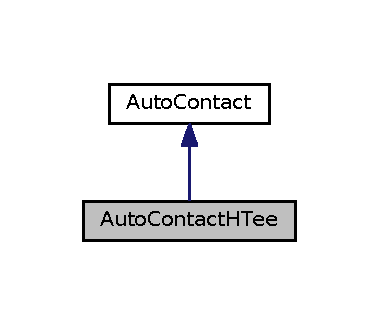
\includegraphics[width=182pt]{classKatabatic_1_1AutoContactHTee__inherit__graph}
\end{center}
\end{figure}
\subsection*{Public Member Functions}
\begin{DoxyCompactItemize}
\item 
virtual \mbox{\hyperlink{classKatabatic_1_1AutoSegment}{Auto\+Segment}} $\ast$ \mbox{\hyperlink{classKatabatic_1_1AutoContactHTee_ac9c9b04e245a1109e297510a3968b7ac}{get\+Opposite}} (const \mbox{\hyperlink{classKatabatic_1_1AutoSegment}{Auto\+Segment}} $\ast$) const
\item 
virtual \mbox{\hyperlink{classKatabatic_1_1AutoSegment}{Auto\+Segment}} $\ast$ \mbox{\hyperlink{classKatabatic_1_1AutoContactHTee_ad99dd549214e43b6509fd8e3aefae919}{get\+Perpandicular}} (const \mbox{\hyperlink{classKatabatic_1_1AutoSegment}{Auto\+Segment}} $\ast$) const
\item 
virtual \mbox{\hyperlink{classKatabatic_1_1AutoSegment}{Auto\+Segment}} $\ast$ \mbox{\hyperlink{classKatabatic_1_1AutoContactHTee_a99fa8a78e97a29f2fb5730eaaa59acfc}{get\+Segment}} (unsigned int) const
\item 
virtual void \mbox{\hyperlink{classKatabatic_1_1AutoContactHTee_a3e218f6934c51380fb15d0e2bd380071}{update\+Geometry}} ()
\item 
virtual void \mbox{\hyperlink{classKatabatic_1_1AutoContactHTee_af5bf1f5e71204ef84346e4e036175431}{update\+Topology}} ()
\end{DoxyCompactItemize}
\subsection*{Static Public Member Functions}
\begin{DoxyCompactItemize}
\item 
static \mbox{\hyperlink{classKatabatic_1_1AutoContactHTee}{Auto\+Contact\+H\+Tee}} $\ast$ \mbox{\hyperlink{classKatabatic_1_1AutoContactHTee_a9b42579ac2487765c83e31f7ca3ee562}{create}} (\mbox{\hyperlink{classKatabatic_1_1GCell}{G\+Cell}} $\ast$, \textbf{ Net} $\ast$, const \textbf{ Layer} $\ast$)
\end{DoxyCompactItemize}
\subsection*{Additional Inherited Members}


\subsection{Detailed Description}
\mbox{\hyperlink{classKatabatic_1_1AutoContact}{Auto\+Contact}} H-\/\+Tee (two H, one V) 

\mbox{\hyperlink{classKatabatic_1_1AutoContact}{Auto\+Contact}} to build an horizontal tee (two H, one V). 

\subsection{Member Function Documentation}
\mbox{\Hypertarget{classKatabatic_1_1AutoContactHTee_a9b42579ac2487765c83e31f7ca3ee562}\label{classKatabatic_1_1AutoContactHTee_a9b42579ac2487765c83e31f7ca3ee562}} 
\index{Katabatic\+::\+Auto\+Contact\+H\+Tee@{Katabatic\+::\+Auto\+Contact\+H\+Tee}!create@{create}}
\index{create@{create}!Katabatic\+::\+Auto\+Contact\+H\+Tee@{Katabatic\+::\+Auto\+Contact\+H\+Tee}}
\subsubsection{\texorpdfstring{create()}{create()}}
{\footnotesize\ttfamily \mbox{\hyperlink{classKatabatic_1_1AutoContactHTee}{Auto\+Contact\+H\+Tee}} $\ast$ create (\begin{DoxyParamCaption}\item[{\mbox{\hyperlink{classKatabatic_1_1GCell}{G\+Cell}} $\ast$}]{gcell,  }\item[{\textbf{ Net} $\ast$}]{net,  }\item[{const \textbf{ Layer} $\ast$}]{layer }\end{DoxyParamCaption})\hspace{0.3cm}{\ttfamily [static]}}


\begin{DoxyParams}{Parameters}
{\em gcell} & The \mbox{\hyperlink{classKatabatic_1_1GCell}{G\+Cell}} into which create the \mbox{\hyperlink{classKatabatic_1_1AutoContact}{Auto\+Contact}}. \\
\hline
{\em net} & The Net to which this \mbox{\hyperlink{classKatabatic_1_1AutoContact}{Auto\+Contact}} belongs. \\
\hline
{\em layer} & The Layer of the \mbox{\hyperlink{classKatabatic_1_1AutoContact}{Auto\+Contact}}. \\
\hline
\end{DoxyParams}
\begin{DoxyReturn}{Returns}
The created \mbox{\hyperlink{classKatabatic_1_1AutoContactHTee}{Auto\+Contact\+H\+Tee}}.
\end{DoxyReturn}
Create a new \mbox{\hyperlink{classKatabatic_1_1AutoContactHTee}{Auto\+Contact\+H\+Tee}}. 

References Katabatic\+::\+Cnt\+In\+Creation\+Stage, and Contact\+::create().



Referenced by G\+Cell\+Topology\+::\+\_\+do\+\_\+x\+G(), G\+Cell\+Topology\+::\+\_\+do\+\_\+x\+G\+\_\+1\+M1\+\_\+1\+M2(), and G\+Cell\+Topology\+::\+\_\+do\+\_\+x\+G\+\_\+x\+M1\+\_\+x\+M3().

\mbox{\Hypertarget{classKatabatic_1_1AutoContactHTee_ac9c9b04e245a1109e297510a3968b7ac}\label{classKatabatic_1_1AutoContactHTee_ac9c9b04e245a1109e297510a3968b7ac}} 
\index{Katabatic\+::\+Auto\+Contact\+H\+Tee@{Katabatic\+::\+Auto\+Contact\+H\+Tee}!get\+Opposite@{get\+Opposite}}
\index{get\+Opposite@{get\+Opposite}!Katabatic\+::\+Auto\+Contact\+H\+Tee@{Katabatic\+::\+Auto\+Contact\+H\+Tee}}
\subsubsection{\texorpdfstring{get\+Opposite()}{getOpposite()}}
{\footnotesize\ttfamily \mbox{\hyperlink{classKatabatic_1_1AutoSegment}{Auto\+Segment}} $\ast$ get\+Opposite (\begin{DoxyParamCaption}\item[{const \mbox{\hyperlink{classKatabatic_1_1AutoSegment}{Auto\+Segment}} $\ast$}]{reference }\end{DoxyParamCaption}) const\hspace{0.3cm}{\ttfamily [virtual]}}

{\bfseries Returns\+:} The other \mbox{\hyperlink{classKatabatic_1_1AutoSegment}{Auto\+Segment}} the {\itshape same} direction as {\ttfamily reference}, this is only meaningful on \mbox{\hyperlink{classKatabatic_1_1AutoContactHTee}{Auto\+Contact\+H\+Tee}} or \mbox{\hyperlink{classKatabatic_1_1AutoContactVTee}{Auto\+Contact\+V\+Tee}}. If there is no opposite, {\ttfamily N\+U\+LL} is returned. 

Implements \mbox{\hyperlink{classKatabatic_1_1AutoContact_a48ab1d3bdf85712e4784ef83ef136939}{Auto\+Contact}}.

\mbox{\Hypertarget{classKatabatic_1_1AutoContactHTee_ad99dd549214e43b6509fd8e3aefae919}\label{classKatabatic_1_1AutoContactHTee_ad99dd549214e43b6509fd8e3aefae919}} 
\index{Katabatic\+::\+Auto\+Contact\+H\+Tee@{Katabatic\+::\+Auto\+Contact\+H\+Tee}!get\+Perpandicular@{get\+Perpandicular}}
\index{get\+Perpandicular@{get\+Perpandicular}!Katabatic\+::\+Auto\+Contact\+H\+Tee@{Katabatic\+::\+Auto\+Contact\+H\+Tee}}
\subsubsection{\texorpdfstring{get\+Perpandicular()}{getPerpandicular()}}
{\footnotesize\ttfamily \mbox{\hyperlink{classKatabatic_1_1AutoSegment}{Auto\+Segment}} $\ast$ get\+Perpandicular (\begin{DoxyParamCaption}\item[{const \mbox{\hyperlink{classKatabatic_1_1AutoSegment}{Auto\+Segment}} $\ast$}]{reference }\end{DoxyParamCaption}) const\hspace{0.3cm}{\ttfamily [virtual]}}

{\bfseries Returns\+:} The \mbox{\hyperlink{classKatabatic_1_1AutoSegment}{Auto\+Segment}} in the {\itshape perpandicular} direction to {\ttfamily reference}, this is only meaningful on Auto\+Contac\+Turn. It there is no unique perpandicular, {\ttfamily N\+U\+LL} is returned. 

Implements \mbox{\hyperlink{classKatabatic_1_1AutoContact_a994371005874f946cc0ac78005d38423}{Auto\+Contact}}.

\mbox{\Hypertarget{classKatabatic_1_1AutoContactHTee_a99fa8a78e97a29f2fb5730eaaa59acfc}\label{classKatabatic_1_1AutoContactHTee_a99fa8a78e97a29f2fb5730eaaa59acfc}} 
\index{Katabatic\+::\+Auto\+Contact\+H\+Tee@{Katabatic\+::\+Auto\+Contact\+H\+Tee}!get\+Segment@{get\+Segment}}
\index{get\+Segment@{get\+Segment}!Katabatic\+::\+Auto\+Contact\+H\+Tee@{Katabatic\+::\+Auto\+Contact\+H\+Tee}}
\subsubsection{\texorpdfstring{get\+Segment()}{getSegment()}}
{\footnotesize\ttfamily \mbox{\hyperlink{classKatabatic_1_1AutoSegment}{Auto\+Segment}} $\ast$ get\+Segment (\begin{DoxyParamCaption}\item[{unsigned int}]{index }\end{DoxyParamCaption}) const\hspace{0.3cm}{\ttfamily [virtual]}}

{\bfseries Returns\+:} The nth anchored \mbox{\hyperlink{classKatabatic_1_1AutoSegment}{Auto\+Segment}}. The index is significant\+:
\begin{DoxyItemize}
\item {\bfseries 0} \+: first horizontal ({\bfseries h1}).
\item {\bfseries 1} \+: second horizontal ({\bfseries h2}).
\item {\bfseries 2} \+: first vertical ({\bfseries b1}).
\item {\bfseries 3} \+: second vertical ({\bfseries b2}).
\end{DoxyItemize}

Not all the indexes are filled for every \mbox{\hyperlink{classKatabatic_1_1AutoContact}{Auto\+Contact}}. For example {\ttfamily Turn} have {\bfseries h1} and {\bfseries b1}, and {\ttfamily H\+Tee} have {\bfseries h1}, {\bfseries h2} and {\bfseries v1}. 

Implements \mbox{\hyperlink{classKatabatic_1_1AutoContact_a50531ded68cc5206fe104b8d8bf3bd87}{Auto\+Contact}}.

\mbox{\Hypertarget{classKatabatic_1_1AutoContactHTee_a3e218f6934c51380fb15d0e2bd380071}\label{classKatabatic_1_1AutoContactHTee_a3e218f6934c51380fb15d0e2bd380071}} 
\index{Katabatic\+::\+Auto\+Contact\+H\+Tee@{Katabatic\+::\+Auto\+Contact\+H\+Tee}!update\+Geometry@{update\+Geometry}}
\index{update\+Geometry@{update\+Geometry}!Katabatic\+::\+Auto\+Contact\+H\+Tee@{Katabatic\+::\+Auto\+Contact\+H\+Tee}}
\subsubsection{\texorpdfstring{update\+Geometry()}{updateGeometry()}}
{\footnotesize\ttfamily void update\+Geometry (\begin{DoxyParamCaption}{ }\end{DoxyParamCaption})\hspace{0.3cm}{\ttfamily [virtual]}}

Compute the new position of the \mbox{\hyperlink{classKatabatic_1_1AutoContact}{Auto\+Contact}} based on the \mbox{\hyperlink{classKatabatic_1_1AutoSegment}{Auto\+Segment}} positions. The \mbox{\hyperlink{classKatabatic_1_1Session}{Session}} mechanism ensure that all \mbox{\hyperlink{classKatabatic_1_1AutoSegment}{Auto\+Segment}} are set into their final positions before calling this updator. 

Implements \mbox{\hyperlink{classKatabatic_1_1AutoContact_af6a2454547eeb7f5a519970dcb467e90}{Auto\+Contact}}.



References Auto\+Contact\+::base(), Debug\+Session\+::close(), Katabatic\+::\+Cnt\+Invalidated, Auto\+Contact\+::get\+Net(), Auto\+Contact\+::get\+X(), Auto\+Contact\+::get\+Y(), Auto\+Contact\+::has\+Bad\+Topology(), Go\+::invalidate(), Auto\+Contact\+::is\+Invalidated\+Cache(), Debug\+Session\+::open(), Auto\+Contact\+::set\+X(), and Auto\+Contact\+::set\+Y().

\mbox{\Hypertarget{classKatabatic_1_1AutoContactHTee_af5bf1f5e71204ef84346e4e036175431}\label{classKatabatic_1_1AutoContactHTee_af5bf1f5e71204ef84346e4e036175431}} 
\index{Katabatic\+::\+Auto\+Contact\+H\+Tee@{Katabatic\+::\+Auto\+Contact\+H\+Tee}!update\+Topology@{update\+Topology}}
\index{update\+Topology@{update\+Topology}!Katabatic\+::\+Auto\+Contact\+H\+Tee@{Katabatic\+::\+Auto\+Contact\+H\+Tee}}
\subsubsection{\texorpdfstring{update\+Topology()}{updateTopology()}}
{\footnotesize\ttfamily void update\+Topology (\begin{DoxyParamCaption}{ }\end{DoxyParamCaption})\hspace{0.3cm}{\ttfamily [virtual]}}

Restore the topology (i.\+e. connexity) of the contact after any number of connected segments has changed layer (at least one, up to three).

For any configuration, the connexity can be restored by making only one dogleg.

We distinguish two kind of layer changes\+:
\begin{DoxyEnumerate}
\item The two horizontals ({\ttfamily h1} and {\ttfamily h2}) are still on the same layer (either they both moved or the vertical only has moved, see figures 2 \& 4). In that case, the dogleg is made on the vertical.
\item The two horizontals no longer are on the same layer (figures 1 \& 3). In that case, the dogleg is made on the horizontal which is at the greater distance (in a layer sense) from the vertical.
\end{DoxyEnumerate}

 

Implements \mbox{\hyperlink{classKatabatic_1_1AutoContact_a690764ddc997fe9766a79c4b8e0c3e2f}{Auto\+Contact}}.



References Debug\+Session\+::close(), Katabatic\+::\+Cnt\+Bad\+Topology, Routing\+Gauge\+::get\+Contact\+Layer(), Auto\+Contact\+::get\+Layer(), Routing\+Gauge\+::get\+Layer\+Depth(), Auto\+Contact\+::get\+Net(), Session\+::get\+Routing\+Gauge(), Routing\+Gauge\+::get\+Routing\+Layer(), Auto\+Contact\+::has\+Bad\+Topology(), Auto\+Contact\+::is\+Invalidated\+Cache(), Debug\+Session\+::open(), Auto\+Contact\+::set\+Layer(), and Auto\+Contact\+::show\+Topology\+Error().



The documentation for this class was generated from the following files\+:\begin{DoxyCompactItemize}
\item 
Auto\+Contact\+H\+Tee.\+h\item 
Auto\+Contact\+H\+Tee.\+cpp\item 
Auto\+Contact\+H\+Tee.\+dox\end{DoxyCompactItemize}

\hypertarget{classKatabatic_1_1AutoContactTerminal}{}\section{Auto\+Contact\+Terminal Class Reference}
\label{classKatabatic_1_1AutoContactTerminal}\index{Auto\+Contact\+Terminal@{Auto\+Contact\+Terminal}}


\mbox{\hyperlink{classKatabatic_1_1AutoContact}{Auto\+Contact}} Terminal (S/T is a Terminal)  




Inheritance diagram for Auto\+Contact\+Terminal\+:\nopagebreak
\begin{figure}[H]
\begin{center}
\leavevmode
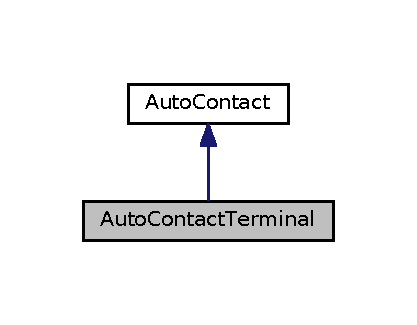
\includegraphics[width=200pt]{classKatabatic_1_1AutoContactTerminal__inherit__graph}
\end{center}
\end{figure}
\subsection*{Public Member Functions}
\begin{DoxyCompactItemize}
\item 
virtual \textbf{ Box} \mbox{\hyperlink{classKatabatic_1_1AutoContactTerminal_a00ed934305dd186a284b7a13b5798cb6}{get\+Native\+Constraint\+Box}} () const
\item 
virtual \mbox{\hyperlink{classKatabatic_1_1AutoSegment}{Auto\+Segment}} $\ast$ \mbox{\hyperlink{classKatabatic_1_1AutoContactTerminal_a99fa8a78e97a29f2fb5730eaaa59acfc}{get\+Segment}} (unsigned int) const
\item 
virtual \mbox{\hyperlink{classKatabatic_1_1AutoSegment}{Auto\+Segment}} $\ast$ \mbox{\hyperlink{classKatabatic_1_1AutoContactTerminal_ac9c9b04e245a1109e297510a3968b7ac}{get\+Opposite}} (const \mbox{\hyperlink{classKatabatic_1_1AutoSegment}{Auto\+Segment}} $\ast$) const
\item 
virtual \mbox{\hyperlink{classKatabatic_1_1AutoSegment}{Auto\+Segment}} $\ast$ \mbox{\hyperlink{classKatabatic_1_1AutoContactTerminal_ad99dd549214e43b6509fd8e3aefae919}{get\+Perpandicular}} (const \mbox{\hyperlink{classKatabatic_1_1AutoSegment}{Auto\+Segment}} $\ast$) const
\item 
virtual void \mbox{\hyperlink{classKatabatic_1_1AutoContactTerminal_a3e218f6934c51380fb15d0e2bd380071}{update\+Geometry}} ()
\item 
virtual void \mbox{\hyperlink{classKatabatic_1_1AutoContactTerminal_af5bf1f5e71204ef84346e4e036175431}{update\+Topology}} ()
\end{DoxyCompactItemize}
\subsection*{Static Public Member Functions}
\begin{DoxyCompactItemize}
\item 
static \mbox{\hyperlink{classKatabatic_1_1AutoContactTerminal}{Auto\+Contact\+Terminal}} $\ast$ \mbox{\hyperlink{classKatabatic_1_1AutoContactTerminal_a0d440e51525b09acc843f1d345850487}{create}} (\mbox{\hyperlink{classKatabatic_1_1GCell}{G\+Cell}} $\ast$gcell, \textbf{ Component} $\ast$anchor, const \textbf{ Layer} $\ast$layer, \textbf{ Point} point, \textbf{ Db\+U\+::\+Unit} width, \textbf{ Db\+U\+::\+Unit} height)
\item 
static \mbox{\hyperlink{classKatabatic_1_1AutoContactTerminal}{Auto\+Contact\+Terminal}} $\ast$ \mbox{\hyperlink{classKatabatic_1_1AutoContactTerminal_a60a625bca2cdfebcdcc7826ab781d1bb}{create}} (\mbox{\hyperlink{classKatabatic_1_1GCell}{G\+Cell}} $\ast$gcell, \textbf{ Component} $\ast$anchor, const \textbf{ Layer} $\ast$layer, const \textbf{ Db\+U\+::\+Unit} dx, const \textbf{ Db\+U\+::\+Unit} dy, const \textbf{ Db\+U\+::\+Unit} width, const \textbf{ Db\+U\+::\+Unit} height)
\end{DoxyCompactItemize}
\subsection*{Additional Inherited Members}


\subsection{Detailed Description}
\mbox{\hyperlink{classKatabatic_1_1AutoContact}{Auto\+Contact}} Terminal (S/T is a Terminal) 

\mbox{\hyperlink{classKatabatic_1_1AutoContact}{Auto\+Contact}} that are directly attached by either source or target or both to a terminal. 

\subsection{Member Function Documentation}
\mbox{\Hypertarget{classKatabatic_1_1AutoContactTerminal_a0d440e51525b09acc843f1d345850487}\label{classKatabatic_1_1AutoContactTerminal_a0d440e51525b09acc843f1d345850487}} 
\index{Katabatic\+::\+Auto\+Contact\+Terminal@{Katabatic\+::\+Auto\+Contact\+Terminal}!create@{create}}
\index{create@{create}!Katabatic\+::\+Auto\+Contact\+Terminal@{Katabatic\+::\+Auto\+Contact\+Terminal}}
\subsubsection{\texorpdfstring{create()}{create()}\hspace{0.1cm}{\footnotesize\ttfamily [1/2]}}
{\footnotesize\ttfamily \mbox{\hyperlink{classKatabatic_1_1AutoContactTerminal}{Auto\+Contact\+Terminal}} $\ast$ create (\begin{DoxyParamCaption}\item[{\mbox{\hyperlink{classKatabatic_1_1GCell}{G\+Cell}} $\ast$}]{gcell,  }\item[{\textbf{ Component} $\ast$}]{rp,  }\item[{const \textbf{ Layer} $\ast$}]{layer,  }\item[{\textbf{ Point}}]{point,  }\item[{\textbf{ Db\+U\+::\+Unit}}]{width,  }\item[{\textbf{ Db\+U\+::\+Unit}}]{height }\end{DoxyParamCaption})\hspace{0.3cm}{\ttfamily [static]}}


\begin{DoxyParams}{Parameters}
{\em gcell} & The \mbox{\hyperlink{classKatabatic_1_1GCell}{G\+Cell}} into which create the \mbox{\hyperlink{classKatabatic_1_1AutoContact}{Auto\+Contact}}. \\
\hline
{\em rp} & The Routing\+Pad on which to anchor the \mbox{\hyperlink{classKatabatic_1_1AutoContact}{Auto\+Contact}}. \\
\hline
{\em layer} & The Layer of the \mbox{\hyperlink{classKatabatic_1_1AutoContact}{Auto\+Contact}}. \\
\hline
{\em point} & The absolute position. \\
\hline
{\em width} & The width of the \mbox{\hyperlink{classKatabatic_1_1AutoContact}{Auto\+Contact}}. \\
\hline
{\em height} & The height of the \mbox{\hyperlink{classKatabatic_1_1AutoContact}{Auto\+Contact}}. \\
\hline
\end{DoxyParams}
\begin{DoxyReturn}{Returns}
The created \mbox{\hyperlink{classKatabatic_1_1AutoContact}{Auto\+Contact}}.
\end{DoxyReturn}
Create a new \mbox{\hyperlink{classKatabatic_1_1AutoContactTerminal}{Auto\+Contact\+Terminal}} anchored on {\ttfamily rp}. {\ttfamily point} gives the {\itshape absolute} position. 

References Hook\+::detach(), and Component\+::get\+Body\+Hook().



Referenced by G\+Cell\+Topology\+::do\+Rp\+\_\+\+Access\+Pad(), and G\+Cell\+Topology\+::do\+Rp\+\_\+\+Auto\+Contacts().

\mbox{\Hypertarget{classKatabatic_1_1AutoContactTerminal_a60a625bca2cdfebcdcc7826ab781d1bb}\label{classKatabatic_1_1AutoContactTerminal_a60a625bca2cdfebcdcc7826ab781d1bb}} 
\index{Katabatic\+::\+Auto\+Contact\+Terminal@{Katabatic\+::\+Auto\+Contact\+Terminal}!create@{create}}
\index{create@{create}!Katabatic\+::\+Auto\+Contact\+Terminal@{Katabatic\+::\+Auto\+Contact\+Terminal}}
\subsubsection{\texorpdfstring{create()}{create()}\hspace{0.1cm}{\footnotesize\ttfamily [2/2]}}
{\footnotesize\ttfamily \mbox{\hyperlink{classKatabatic_1_1AutoContactTerminal}{Auto\+Contact\+Terminal}} $\ast$ create (\begin{DoxyParamCaption}\item[{\mbox{\hyperlink{classKatabatic_1_1GCell}{G\+Cell}} $\ast$}]{gcell,  }\item[{\textbf{ Component} $\ast$}]{rp,  }\item[{const \textbf{ Layer} $\ast$}]{layer,  }\item[{const \textbf{ Db\+U\+::\+Unit}}]{x,  }\item[{const \textbf{ Db\+U\+::\+Unit}}]{y,  }\item[{const \textbf{ Db\+U\+::\+Unit}}]{width,  }\item[{const \textbf{ Db\+U\+::\+Unit}}]{height }\end{DoxyParamCaption})\hspace{0.3cm}{\ttfamily [static]}}


\begin{DoxyParams}{Parameters}
{\em gcell} & The \mbox{\hyperlink{classKatabatic_1_1GCell}{G\+Cell}} into which create the \mbox{\hyperlink{classKatabatic_1_1AutoContact}{Auto\+Contact}}. \\
\hline
{\em rp} & The Component on which to anchor the \mbox{\hyperlink{classKatabatic_1_1AutoContact}{Auto\+Contact}}. \\
\hline
{\em layer} & The Layer of the \mbox{\hyperlink{classKatabatic_1_1AutoContact}{Auto\+Contact}}. \\
\hline
{\em x} & The absolute X position. \\
\hline
{\em y} & The absolute Y position. \\
\hline
{\em width} & The width of the \mbox{\hyperlink{classKatabatic_1_1AutoContact}{Auto\+Contact}}. \\
\hline
{\em height} & The height of the \mbox{\hyperlink{classKatabatic_1_1AutoContact}{Auto\+Contact}}. \\
\hline
\end{DoxyParams}
\begin{DoxyReturn}{Returns}
The created \mbox{\hyperlink{classKatabatic_1_1AutoContact}{Auto\+Contact}}.
\end{DoxyReturn}
Create a new \mbox{\hyperlink{classKatabatic_1_1AutoContactTerminal}{Auto\+Contact\+Terminal}} anchored on {\ttfamily rp}. {\ttfamily (x,y)} gives the {\itshape absolute} position.

The anchor component {\ttfamily rp} is most often a \textbf{ Hurricane\+::\+Routing\+Pad} (occurrencing a \textbf{ Hurricane\+::\+Segment}) or directly a \textbf{ Hurricane\+::\+Segment}, in case of Routing\+Pad layer promotion. 

References Katabatic\+::\+Cnt\+In\+Creation\+Stage, Contact\+::create(), Component\+::get\+Position(), and Db\+U\+::get\+Value\+String().

\mbox{\Hypertarget{classKatabatic_1_1AutoContactTerminal_a00ed934305dd186a284b7a13b5798cb6}\label{classKatabatic_1_1AutoContactTerminal_a00ed934305dd186a284b7a13b5798cb6}} 
\index{Katabatic\+::\+Auto\+Contact\+Terminal@{Katabatic\+::\+Auto\+Contact\+Terminal}!get\+Native\+Constraint\+Box@{get\+Native\+Constraint\+Box}}
\index{get\+Native\+Constraint\+Box@{get\+Native\+Constraint\+Box}!Katabatic\+::\+Auto\+Contact\+Terminal@{Katabatic\+::\+Auto\+Contact\+Terminal}}
\subsubsection{\texorpdfstring{get\+Native\+Constraint\+Box()}{getNativeConstraintBox()}}
{\footnotesize\ttfamily \textbf{ Box} get\+Native\+Constraint\+Box (\begin{DoxyParamCaption}{ }\end{DoxyParamCaption}) const\hspace{0.3cm}{\ttfamily [virtual]}}

{\bfseries Returns\+:} The native constraint box (that is, whithout any user constraints applied). For \mbox{\hyperlink{classKatabatic_1_1AutoContactTerminal}{Auto\+Contact\+Terminal}}, this is the Box of the supporting external component, and for all others the bounding box of the owning \mbox{\hyperlink{classKatabatic_1_1GCell}{G\+Cell}}. 

Reimplemented from \mbox{\hyperlink{classKatabatic_1_1AutoContact_a00ed934305dd186a284b7a13b5798cb6}{Auto\+Contact}}.



References Auto\+Contact\+::get\+Anchor(), G\+Cell\+::get\+Bounding\+Box(), Occurrence\+::get\+Entity(), Routing\+Pad\+::get\+Occurrence(), Transformation\+::get\+Orientation(), Occurrence\+::get\+Path(), Component\+::get\+Position(), Routing\+Pad\+::get\+Source\+Position(), Segment\+::get\+Source\+Position(), Routing\+Pad\+::get\+Target\+Position(), Segment\+::get\+Target\+Position(), Path\+::get\+Transformation(), and Db\+U\+::get\+Value\+String().

\mbox{\Hypertarget{classKatabatic_1_1AutoContactTerminal_a99fa8a78e97a29f2fb5730eaaa59acfc}\label{classKatabatic_1_1AutoContactTerminal_a99fa8a78e97a29f2fb5730eaaa59acfc}} 
\index{Katabatic\+::\+Auto\+Contact\+Terminal@{Katabatic\+::\+Auto\+Contact\+Terminal}!get\+Segment@{get\+Segment}}
\index{get\+Segment@{get\+Segment}!Katabatic\+::\+Auto\+Contact\+Terminal@{Katabatic\+::\+Auto\+Contact\+Terminal}}
\subsubsection{\texorpdfstring{get\+Segment()}{getSegment()}}
{\footnotesize\ttfamily \mbox{\hyperlink{classKatabatic_1_1AutoSegment}{Auto\+Segment}} $\ast$ get\+Segment (\begin{DoxyParamCaption}\item[{unsigned int}]{index }\end{DoxyParamCaption}) const\hspace{0.3cm}{\ttfamily [virtual]}}

{\bfseries Returns\+:} The nth anchored \mbox{\hyperlink{classKatabatic_1_1AutoSegment}{Auto\+Segment}}. The index is significant\+:
\begin{DoxyItemize}
\item {\bfseries 0} \+: first horizontal ({\bfseries h1}).
\item {\bfseries 1} \+: second horizontal ({\bfseries h2}).
\item {\bfseries 2} \+: first vertical ({\bfseries b1}).
\item {\bfseries 3} \+: second vertical ({\bfseries b2}).
\end{DoxyItemize}

Not all the indexes are filled for every \mbox{\hyperlink{classKatabatic_1_1AutoContact}{Auto\+Contact}}. For example {\ttfamily Turn} have {\bfseries h1} and {\bfseries b1}, and {\ttfamily H\+Tee} have {\bfseries h1}, {\bfseries h2} and {\bfseries v1}. 

Implements \mbox{\hyperlink{classKatabatic_1_1AutoContact_a50531ded68cc5206fe104b8d8bf3bd87}{Auto\+Contact}}.



References Auto\+Segment\+::is\+Horizontal(), and Auto\+Segment\+::is\+Vertical().

\mbox{\Hypertarget{classKatabatic_1_1AutoContactTerminal_ac9c9b04e245a1109e297510a3968b7ac}\label{classKatabatic_1_1AutoContactTerminal_ac9c9b04e245a1109e297510a3968b7ac}} 
\index{Katabatic\+::\+Auto\+Contact\+Terminal@{Katabatic\+::\+Auto\+Contact\+Terminal}!get\+Opposite@{get\+Opposite}}
\index{get\+Opposite@{get\+Opposite}!Katabatic\+::\+Auto\+Contact\+Terminal@{Katabatic\+::\+Auto\+Contact\+Terminal}}
\subsubsection{\texorpdfstring{get\+Opposite()}{getOpposite()}}
{\footnotesize\ttfamily \mbox{\hyperlink{classKatabatic_1_1AutoSegment}{Auto\+Segment}} $\ast$ get\+Opposite (\begin{DoxyParamCaption}\item[{const \mbox{\hyperlink{classKatabatic_1_1AutoSegment}{Auto\+Segment}} $\ast$}]{reference }\end{DoxyParamCaption}) const\hspace{0.3cm}{\ttfamily [virtual]}}

{\bfseries Returns\+:} The other \mbox{\hyperlink{classKatabatic_1_1AutoSegment}{Auto\+Segment}} the {\itshape same} direction as {\ttfamily reference}, this is only meaningful on \mbox{\hyperlink{classKatabatic_1_1AutoContactHTee}{Auto\+Contact\+H\+Tee}} or \mbox{\hyperlink{classKatabatic_1_1AutoContactVTee}{Auto\+Contact\+V\+Tee}}. If there is no opposite, {\ttfamily N\+U\+LL} is returned. 

Implements \mbox{\hyperlink{classKatabatic_1_1AutoContact_a48ab1d3bdf85712e4784ef83ef136939}{Auto\+Contact}}.

\mbox{\Hypertarget{classKatabatic_1_1AutoContactTerminal_ad99dd549214e43b6509fd8e3aefae919}\label{classKatabatic_1_1AutoContactTerminal_ad99dd549214e43b6509fd8e3aefae919}} 
\index{Katabatic\+::\+Auto\+Contact\+Terminal@{Katabatic\+::\+Auto\+Contact\+Terminal}!get\+Perpandicular@{get\+Perpandicular}}
\index{get\+Perpandicular@{get\+Perpandicular}!Katabatic\+::\+Auto\+Contact\+Terminal@{Katabatic\+::\+Auto\+Contact\+Terminal}}
\subsubsection{\texorpdfstring{get\+Perpandicular()}{getPerpandicular()}}
{\footnotesize\ttfamily \mbox{\hyperlink{classKatabatic_1_1AutoSegment}{Auto\+Segment}} $\ast$ get\+Perpandicular (\begin{DoxyParamCaption}\item[{const \mbox{\hyperlink{classKatabatic_1_1AutoSegment}{Auto\+Segment}} $\ast$}]{reference }\end{DoxyParamCaption}) const\hspace{0.3cm}{\ttfamily [virtual]}}

{\bfseries Returns\+:} The \mbox{\hyperlink{classKatabatic_1_1AutoSegment}{Auto\+Segment}} in the {\itshape perpandicular} direction to {\ttfamily reference}, this is only meaningful on Auto\+Contac\+Turn. It there is no unique perpandicular, {\ttfamily N\+U\+LL} is returned. 

Implements \mbox{\hyperlink{classKatabatic_1_1AutoContact_a994371005874f946cc0ac78005d38423}{Auto\+Contact}}.

\mbox{\Hypertarget{classKatabatic_1_1AutoContactTerminal_a3e218f6934c51380fb15d0e2bd380071}\label{classKatabatic_1_1AutoContactTerminal_a3e218f6934c51380fb15d0e2bd380071}} 
\index{Katabatic\+::\+Auto\+Contact\+Terminal@{Katabatic\+::\+Auto\+Contact\+Terminal}!update\+Geometry@{update\+Geometry}}
\index{update\+Geometry@{update\+Geometry}!Katabatic\+::\+Auto\+Contact\+Terminal@{Katabatic\+::\+Auto\+Contact\+Terminal}}
\subsubsection{\texorpdfstring{update\+Geometry()}{updateGeometry()}}
{\footnotesize\ttfamily void update\+Geometry (\begin{DoxyParamCaption}{ }\end{DoxyParamCaption})\hspace{0.3cm}{\ttfamily [virtual]}}

Compute the new position of the \mbox{\hyperlink{classKatabatic_1_1AutoContact}{Auto\+Contact}} based on the \mbox{\hyperlink{classKatabatic_1_1AutoSegment}{Auto\+Segment}} positions. The \mbox{\hyperlink{classKatabatic_1_1Session}{Session}} mechanism ensure that all \mbox{\hyperlink{classKatabatic_1_1AutoSegment}{Auto\+Segment}} are set into their final positions before calling this updator. 

Implements \mbox{\hyperlink{classKatabatic_1_1AutoContact_af6a2454547eeb7f5a519970dcb467e90}{Auto\+Contact}}.



References Auto\+Contact\+::base(), Debug\+Session\+::close(), Katabatic\+::\+Cnt\+Invalidated, Interval\+::contains(), Auto\+Contact\+::get\+Net(), Auto\+Contact\+::get\+U\+Constraints(), Db\+U\+::get\+Value\+String(), Auto\+Segment\+::get\+X(), Auto\+Segment\+::get\+Y(), Auto\+Contact\+::has\+Bad\+Topology(), Go\+::invalidate(), Auto\+Segment\+::is\+Created(), Auto\+Segment\+::is\+Horizontal(), Auto\+Contact\+::is\+Invalidated\+Cache(), Katabatic\+::\+Kb\+Horizontal, Katabatic\+::\+Kb\+Vertical, Debug\+Session\+::open(), Auto\+Contact\+::set\+X(), Auto\+Contact\+::set\+Y(), and Auto\+Contact\+::show\+Topology\+Error().

\mbox{\Hypertarget{classKatabatic_1_1AutoContactTerminal_af5bf1f5e71204ef84346e4e036175431}\label{classKatabatic_1_1AutoContactTerminal_af5bf1f5e71204ef84346e4e036175431}} 
\index{Katabatic\+::\+Auto\+Contact\+Terminal@{Katabatic\+::\+Auto\+Contact\+Terminal}!update\+Topology@{update\+Topology}}
\index{update\+Topology@{update\+Topology}!Katabatic\+::\+Auto\+Contact\+Terminal@{Katabatic\+::\+Auto\+Contact\+Terminal}}
\subsubsection{\texorpdfstring{update\+Topology()}{updateTopology()}}
{\footnotesize\ttfamily void update\+Topology (\begin{DoxyParamCaption}{ }\end{DoxyParamCaption})\hspace{0.3cm}{\ttfamily [virtual]}}

Restore the topology (i.\+e. connexity) of the contact after the incident segment has changed layer.

Based on the layer depth delta between the terminal and the segment three case can occurs\+:
\begin{DoxyItemize}
\item The delta is {\bfseries zero}, then just sets the layer of the contact to the common metal layer.
\item The delta is {\bfseries one}, then sets the contact layer to V\+IA connecting the two layers.
\item The delta is {\bfseries two}, then create a dogleg to restore the connexity. Depending on whether the terminal was attached to the source or target, sets the layer of the segments.
\item A delta of more than {\bfseries two} is an error, and must never occurs.
\end{DoxyItemize}

As, by default, the perpandicular is set in the layer above the parallel, it may be necessary to adjust his layer as well (to the one below).

 

Implements \mbox{\hyperlink{classKatabatic_1_1AutoContact_a690764ddc997fe9766a79c4b8e0c3e2f}{Auto\+Contact}}.



References Debug\+Session\+::close(), Katabatic\+::\+Cnt\+Bad\+Topology, Auto\+Contact\+::get\+Anchor(), Routing\+Gauge\+::get\+Contact\+Layer(), Auto\+Contact\+::get\+Layer(), Auto\+Segment\+::get\+Layer(), Routing\+Gauge\+::get\+Layer\+Depth(), Auto\+Contact\+::get\+Net(), Session\+::get\+Routing\+Gauge(), Routing\+Gauge\+::get\+Routing\+Layer(), Auto\+Segment\+::invalidate(), Auto\+Contact\+::is\+Invalidated\+Cache(), Auto\+Segment\+::make\+Dogleg(), Debug\+Session\+::open(), Auto\+Contact\+::set\+Layer(), and Auto\+Contact\+::show\+Topology\+Error().



The documentation for this class was generated from the following files\+:\begin{DoxyCompactItemize}
\item 
Auto\+Contact\+Terminal.\+h\item 
Auto\+Contact\+Terminal.\+cpp\item 
Auto\+Contact\+Terminal.\+dox\end{DoxyCompactItemize}

\hypertarget{classKatabatic_1_1AutoContactTurn}{}\section{Auto\+Contact\+Turn Class Reference}
\label{classKatabatic_1_1AutoContactTurn}\index{Auto\+Contact\+Turn@{Auto\+Contact\+Turn}}


\mbox{\hyperlink{classKatabatic_1_1AutoContact}{Auto\+Contact}} Turn (one H, one V)  




Inheritance diagram for Auto\+Contact\+Turn\+:\nopagebreak
\begin{figure}[H]
\begin{center}
\leavevmode
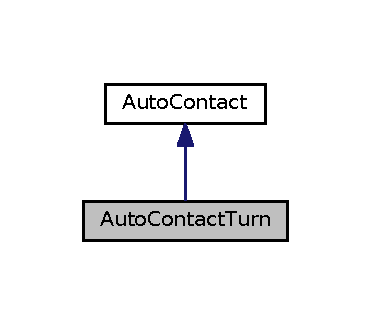
\includegraphics[width=178pt]{classKatabatic_1_1AutoContactTurn__inherit__graph}
\end{center}
\end{figure}
\subsection*{Public Member Functions}
\begin{DoxyCompactItemize}
\item 
virtual \mbox{\hyperlink{classKatabatic_1_1AutoSegment}{Auto\+Segment}} $\ast$ \mbox{\hyperlink{classKatabatic_1_1AutoContactTurn_ac9c9b04e245a1109e297510a3968b7ac}{get\+Opposite}} (const \mbox{\hyperlink{classKatabatic_1_1AutoSegment}{Auto\+Segment}} $\ast$) const
\item 
virtual \mbox{\hyperlink{classKatabatic_1_1AutoSegment}{Auto\+Segment}} $\ast$ \mbox{\hyperlink{classKatabatic_1_1AutoContactTurn_ad99dd549214e43b6509fd8e3aefae919}{get\+Perpandicular}} (const \mbox{\hyperlink{classKatabatic_1_1AutoSegment}{Auto\+Segment}} $\ast$) const
\item 
virtual \mbox{\hyperlink{classKatabatic_1_1AutoSegment}{Auto\+Segment}} $\ast$ \mbox{\hyperlink{classKatabatic_1_1AutoContactTurn_a99fa8a78e97a29f2fb5730eaaa59acfc}{get\+Segment}} (unsigned int) const
\item 
virtual void \mbox{\hyperlink{classKatabatic_1_1AutoContactTurn_a3e218f6934c51380fb15d0e2bd380071}{update\+Geometry}} ()
\item 
virtual void \mbox{\hyperlink{classKatabatic_1_1AutoContactTurn_af5bf1f5e71204ef84346e4e036175431}{update\+Topology}} ()
\end{DoxyCompactItemize}
\subsection*{Static Public Member Functions}
\begin{DoxyCompactItemize}
\item 
static \mbox{\hyperlink{classKatabatic_1_1AutoContactTurn}{Auto\+Contact\+Turn}} $\ast$ \mbox{\hyperlink{classKatabatic_1_1AutoContactTurn_a9d4adb00ccea486f5478bb24e171bdb3}{create}} (\mbox{\hyperlink{classKatabatic_1_1GCell}{G\+Cell}} $\ast$, \textbf{ Net} $\ast$, const \textbf{ Layer} $\ast$)
\end{DoxyCompactItemize}
\subsection*{Additional Inherited Members}


\subsection{Detailed Description}
\mbox{\hyperlink{classKatabatic_1_1AutoContact}{Auto\+Contact}} Turn (one H, one V) 

\mbox{\hyperlink{classKatabatic_1_1AutoContact}{Auto\+Contact}} to make a turn (one H, one V). 

\subsection{Member Function Documentation}
\mbox{\Hypertarget{classKatabatic_1_1AutoContactTurn_a9d4adb00ccea486f5478bb24e171bdb3}\label{classKatabatic_1_1AutoContactTurn_a9d4adb00ccea486f5478bb24e171bdb3}} 
\index{Katabatic\+::\+Auto\+Contact\+Turn@{Katabatic\+::\+Auto\+Contact\+Turn}!create@{create}}
\index{create@{create}!Katabatic\+::\+Auto\+Contact\+Turn@{Katabatic\+::\+Auto\+Contact\+Turn}}
\subsubsection{\texorpdfstring{create()}{create()}}
{\footnotesize\ttfamily \mbox{\hyperlink{classKatabatic_1_1AutoContactTurn}{Auto\+Contact\+Turn}} $\ast$ create (\begin{DoxyParamCaption}\item[{\mbox{\hyperlink{classKatabatic_1_1GCell}{G\+Cell}} $\ast$}]{gcell,  }\item[{\textbf{ Net} $\ast$}]{net,  }\item[{const \textbf{ Layer} $\ast$}]{layer }\end{DoxyParamCaption})\hspace{0.3cm}{\ttfamily [static]}}


\begin{DoxyParams}{Parameters}
{\em gcell} & The \mbox{\hyperlink{classKatabatic_1_1GCell}{G\+Cell}} into which create the \mbox{\hyperlink{classKatabatic_1_1AutoContact}{Auto\+Contact}}. \\
\hline
{\em net} & The Net to which this \mbox{\hyperlink{classKatabatic_1_1AutoContact}{Auto\+Contact}} belongs. \\
\hline
{\em layer} & The Layer of the \mbox{\hyperlink{classKatabatic_1_1AutoContact}{Auto\+Contact}}. \\
\hline
\end{DoxyParams}
\begin{DoxyReturn}{Returns}
The created \mbox{\hyperlink{classKatabatic_1_1AutoContactTurn}{Auto\+Contact\+Turn}}.
\end{DoxyReturn}
Create a new \mbox{\hyperlink{classKatabatic_1_1AutoContactTurn}{Auto\+Contact\+Turn}}. 

References Katabatic\+::\+Cnt\+In\+Creation\+Stage, and Contact\+::create().



Referenced by G\+Cell\+Topology\+::\+\_\+do\+\_\+1\+G\+\_\+1\+M3(), G\+Cell\+Topology\+::\+\_\+do\+\_\+1\+G\+\_\+x\+M1(), G\+Cell\+Topology\+::\+\_\+do\+\_\+x\+G(), G\+Cell\+Topology\+::\+\_\+do\+\_\+x\+G\+\_\+1\+M1\+\_\+1\+M2(), G\+Cell\+Topology\+::\+\_\+do\+\_\+x\+G\+\_\+1\+Pad(), G\+Cell\+Topology\+::\+\_\+do\+\_\+x\+G\+\_\+x\+M1\+\_\+x\+M3(), G\+Cell\+Topology\+::\+\_\+do\+\_\+x\+G\+\_\+x\+M3(), Auto\+Horizontal\+::\+\_\+make\+Dogleg(), Auto\+Vertical\+::\+\_\+make\+Dogleg(), G\+Cell\+Topology\+::do\+Rp\+\_\+\+Access(), G\+Cell\+Topology\+::do\+Rp\+\_\+\+Stair\+Case\+H(), G\+Cell\+Topology\+::do\+Rp\+\_\+\+Stair\+Case\+V(), and anonymous\+\_\+namespace\{\+Load\+Gr\+By\+Net.\+cpp\}\+::single\+G\+Cell().

\mbox{\Hypertarget{classKatabatic_1_1AutoContactTurn_ac9c9b04e245a1109e297510a3968b7ac}\label{classKatabatic_1_1AutoContactTurn_ac9c9b04e245a1109e297510a3968b7ac}} 
\index{Katabatic\+::\+Auto\+Contact\+Turn@{Katabatic\+::\+Auto\+Contact\+Turn}!get\+Opposite@{get\+Opposite}}
\index{get\+Opposite@{get\+Opposite}!Katabatic\+::\+Auto\+Contact\+Turn@{Katabatic\+::\+Auto\+Contact\+Turn}}
\subsubsection{\texorpdfstring{get\+Opposite()}{getOpposite()}}
{\footnotesize\ttfamily \mbox{\hyperlink{classKatabatic_1_1AutoSegment}{Auto\+Segment}} $\ast$ get\+Opposite (\begin{DoxyParamCaption}\item[{const \mbox{\hyperlink{classKatabatic_1_1AutoSegment}{Auto\+Segment}} $\ast$}]{reference }\end{DoxyParamCaption}) const\hspace{0.3cm}{\ttfamily [virtual]}}

{\bfseries Returns\+:} The other \mbox{\hyperlink{classKatabatic_1_1AutoSegment}{Auto\+Segment}} the {\itshape same} direction as {\ttfamily reference}, this is only meaningful on \mbox{\hyperlink{classKatabatic_1_1AutoContactHTee}{Auto\+Contact\+H\+Tee}} or \mbox{\hyperlink{classKatabatic_1_1AutoContactVTee}{Auto\+Contact\+V\+Tee}}. If there is no opposite, {\ttfamily N\+U\+LL} is returned. 

Implements \mbox{\hyperlink{classKatabatic_1_1AutoContact_a48ab1d3bdf85712e4784ef83ef136939}{Auto\+Contact}}.

\mbox{\Hypertarget{classKatabatic_1_1AutoContactTurn_ad99dd549214e43b6509fd8e3aefae919}\label{classKatabatic_1_1AutoContactTurn_ad99dd549214e43b6509fd8e3aefae919}} 
\index{Katabatic\+::\+Auto\+Contact\+Turn@{Katabatic\+::\+Auto\+Contact\+Turn}!get\+Perpandicular@{get\+Perpandicular}}
\index{get\+Perpandicular@{get\+Perpandicular}!Katabatic\+::\+Auto\+Contact\+Turn@{Katabatic\+::\+Auto\+Contact\+Turn}}
\subsubsection{\texorpdfstring{get\+Perpandicular()}{getPerpandicular()}}
{\footnotesize\ttfamily \mbox{\hyperlink{classKatabatic_1_1AutoSegment}{Auto\+Segment}} $\ast$ get\+Perpandicular (\begin{DoxyParamCaption}\item[{const \mbox{\hyperlink{classKatabatic_1_1AutoSegment}{Auto\+Segment}} $\ast$}]{reference }\end{DoxyParamCaption}) const\hspace{0.3cm}{\ttfamily [virtual]}}

{\bfseries Returns\+:} The \mbox{\hyperlink{classKatabatic_1_1AutoSegment}{Auto\+Segment}} in the {\itshape perpandicular} direction to {\ttfamily reference}, this is only meaningful on Auto\+Contac\+Turn. It there is no unique perpandicular, {\ttfamily N\+U\+LL} is returned. 

Implements \mbox{\hyperlink{classKatabatic_1_1AutoContact_a994371005874f946cc0ac78005d38423}{Auto\+Contact}}.

\mbox{\Hypertarget{classKatabatic_1_1AutoContactTurn_a99fa8a78e97a29f2fb5730eaaa59acfc}\label{classKatabatic_1_1AutoContactTurn_a99fa8a78e97a29f2fb5730eaaa59acfc}} 
\index{Katabatic\+::\+Auto\+Contact\+Turn@{Katabatic\+::\+Auto\+Contact\+Turn}!get\+Segment@{get\+Segment}}
\index{get\+Segment@{get\+Segment}!Katabatic\+::\+Auto\+Contact\+Turn@{Katabatic\+::\+Auto\+Contact\+Turn}}
\subsubsection{\texorpdfstring{get\+Segment()}{getSegment()}}
{\footnotesize\ttfamily \mbox{\hyperlink{classKatabatic_1_1AutoSegment}{Auto\+Segment}} $\ast$ get\+Segment (\begin{DoxyParamCaption}\item[{unsigned int}]{index }\end{DoxyParamCaption}) const\hspace{0.3cm}{\ttfamily [virtual]}}

{\bfseries Returns\+:} The nth anchored \mbox{\hyperlink{classKatabatic_1_1AutoSegment}{Auto\+Segment}}. The index is significant\+:
\begin{DoxyItemize}
\item {\bfseries 0} \+: first horizontal ({\bfseries h1}).
\item {\bfseries 1} \+: second horizontal ({\bfseries h2}).
\item {\bfseries 2} \+: first vertical ({\bfseries b1}).
\item {\bfseries 3} \+: second vertical ({\bfseries b2}).
\end{DoxyItemize}

Not all the indexes are filled for every \mbox{\hyperlink{classKatabatic_1_1AutoContact}{Auto\+Contact}}. For example {\ttfamily Turn} have {\bfseries h1} and {\bfseries b1}, and {\ttfamily H\+Tee} have {\bfseries h1}, {\bfseries h2} and {\bfseries v1}. 

Implements \mbox{\hyperlink{classKatabatic_1_1AutoContact_a50531ded68cc5206fe104b8d8bf3bd87}{Auto\+Contact}}.

\mbox{\Hypertarget{classKatabatic_1_1AutoContactTurn_a3e218f6934c51380fb15d0e2bd380071}\label{classKatabatic_1_1AutoContactTurn_a3e218f6934c51380fb15d0e2bd380071}} 
\index{Katabatic\+::\+Auto\+Contact\+Turn@{Katabatic\+::\+Auto\+Contact\+Turn}!update\+Geometry@{update\+Geometry}}
\index{update\+Geometry@{update\+Geometry}!Katabatic\+::\+Auto\+Contact\+Turn@{Katabatic\+::\+Auto\+Contact\+Turn}}
\subsubsection{\texorpdfstring{update\+Geometry()}{updateGeometry()}}
{\footnotesize\ttfamily void update\+Geometry (\begin{DoxyParamCaption}{ }\end{DoxyParamCaption})\hspace{0.3cm}{\ttfamily [virtual]}}

Compute the new position of the \mbox{\hyperlink{classKatabatic_1_1AutoContact}{Auto\+Contact}} based on the \mbox{\hyperlink{classKatabatic_1_1AutoSegment}{Auto\+Segment}} positions. The \mbox{\hyperlink{classKatabatic_1_1Session}{Session}} mechanism ensure that all \mbox{\hyperlink{classKatabatic_1_1AutoSegment}{Auto\+Segment}} are set into their final positions before calling this updator. 

Implements \mbox{\hyperlink{classKatabatic_1_1AutoContact_af6a2454547eeb7f5a519970dcb467e90}{Auto\+Contact}}.



References Auto\+Contact\+::base(), Debug\+Session\+::close(), Katabatic\+::\+Cnt\+Invalidated, Auto\+Contact\+::get\+Net(), Auto\+Contact\+::get\+X(), Auto\+Contact\+::get\+Y(), Auto\+Contact\+::has\+Bad\+Topology(), Go\+::invalidate(), Auto\+Contact\+::is\+Invalidated\+Cache(), Debug\+Session\+::open(), Auto\+Contact\+::set\+X(), and Auto\+Contact\+::set\+Y().

\mbox{\Hypertarget{classKatabatic_1_1AutoContactTurn_af5bf1f5e71204ef84346e4e036175431}\label{classKatabatic_1_1AutoContactTurn_af5bf1f5e71204ef84346e4e036175431}} 
\index{Katabatic\+::\+Auto\+Contact\+Turn@{Katabatic\+::\+Auto\+Contact\+Turn}!update\+Topology@{update\+Topology}}
\index{update\+Topology@{update\+Topology}!Katabatic\+::\+Auto\+Contact\+Turn@{Katabatic\+::\+Auto\+Contact\+Turn}}
\subsubsection{\texorpdfstring{update\+Topology()}{updateTopology()}}
{\footnotesize\ttfamily void update\+Topology (\begin{DoxyParamCaption}{ }\end{DoxyParamCaption})\hspace{0.3cm}{\ttfamily [virtual]}}

Restore the topology (i.\+e. connexity) of the contact after one or both connected segments has changed layer.

Based on the layer depth delta between the two perpandiculars segments. Three case can occurs\+:
\begin{DoxyItemize}
\item The delta is {\bfseries zero}, then just sets the layer of the contact to the common metal layer (turn in same layer).
\item The delta is {\bfseries one}, then sets the contact layer to V\+IA connecting the two layers.
\item The delta {\bfseries cannot be equal to two}, due to the alternatives routing directions, it would mean a {\itshape turn} connecting two {\itshape horizontals} (or verticals) in different layers.
\item The delta is {\bfseries three}, then create a dogleg to restore the connexity. The dogleg will be created on the connected segment which as been {\itshape layer invalidated}. If both of them have been invalidated, the horizontal one is preferred.
\item A delta of more than {\bfseries three} is an error, and must never occurs.
\end{DoxyItemize}

 

Implements \mbox{\hyperlink{classKatabatic_1_1AutoContact_a690764ddc997fe9766a79c4b8e0c3e2f}{Auto\+Contact}}.



References Debug\+Session\+::close(), Katabatic\+::\+Cnt\+Bad\+Topology, Routing\+Gauge\+::get\+Contact\+Layer(), Auto\+Contact\+::get\+Layer(), Auto\+Segment\+::get\+Layer(), Routing\+Gauge\+::get\+Layer\+Depth(), Auto\+Contact\+::get\+Net(), Session\+::get\+Routing\+Gauge(), Routing\+Gauge\+::get\+Routing\+Layer(), Auto\+Contact\+::has\+Bad\+Topology(), Auto\+Segment\+::invalidate(), Auto\+Contact\+::is\+Invalidated\+Cache(), Auto\+Segment\+::is\+Invalidated\+Layer(), Auto\+Segment\+::make\+Dogleg(), Debug\+Session\+::open(), Auto\+Contact\+::set\+Layer(), and Auto\+Contact\+::show\+Topology\+Error().



The documentation for this class was generated from the following files\+:\begin{DoxyCompactItemize}
\item 
Auto\+Contact\+Turn.\+h\item 
Auto\+Contact\+Turn.\+cpp\item 
Auto\+Contact\+Turn.\+dox\end{DoxyCompactItemize}

\hypertarget{classKatabatic_1_1AutoContactVTee}{}\section{Auto\+Contact\+V\+Tee Class Reference}
\label{classKatabatic_1_1AutoContactVTee}\index{Auto\+Contact\+V\+Tee@{Auto\+Contact\+V\+Tee}}


\mbox{\hyperlink{classKatabatic_1_1AutoContact}{Auto\+Contact}} V-\/\+Tee (one H, two V)  




Inheritance diagram for Auto\+Contact\+V\+Tee\+:\nopagebreak
\begin{figure}[H]
\begin{center}
\leavevmode
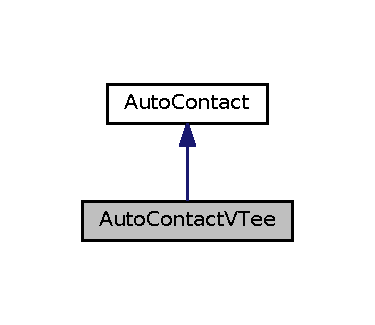
\includegraphics[width=180pt]{classKatabatic_1_1AutoContactVTee__inherit__graph}
\end{center}
\end{figure}
\subsection*{Public Member Functions}
\begin{DoxyCompactItemize}
\item 
virtual \mbox{\hyperlink{classKatabatic_1_1AutoSegment}{Auto\+Segment}} $\ast$ \mbox{\hyperlink{classKatabatic_1_1AutoContactVTee_ac9c9b04e245a1109e297510a3968b7ac}{get\+Opposite}} (const \mbox{\hyperlink{classKatabatic_1_1AutoSegment}{Auto\+Segment}} $\ast$) const
\item 
virtual \mbox{\hyperlink{classKatabatic_1_1AutoSegment}{Auto\+Segment}} $\ast$ \mbox{\hyperlink{classKatabatic_1_1AutoContactVTee_ad99dd549214e43b6509fd8e3aefae919}{get\+Perpandicular}} (const \mbox{\hyperlink{classKatabatic_1_1AutoSegment}{Auto\+Segment}} $\ast$) const
\item 
virtual \mbox{\hyperlink{classKatabatic_1_1AutoSegment}{Auto\+Segment}} $\ast$ \mbox{\hyperlink{classKatabatic_1_1AutoContactVTee_a99fa8a78e97a29f2fb5730eaaa59acfc}{get\+Segment}} (unsigned int) const
\item 
virtual void \mbox{\hyperlink{classKatabatic_1_1AutoContactVTee_a3e218f6934c51380fb15d0e2bd380071}{update\+Geometry}} ()
\item 
virtual void \mbox{\hyperlink{classKatabatic_1_1AutoContactVTee_af5bf1f5e71204ef84346e4e036175431}{update\+Topology}} ()
\end{DoxyCompactItemize}
\subsection*{Static Public Member Functions}
\begin{DoxyCompactItemize}
\item 
static \mbox{\hyperlink{classKatabatic_1_1AutoContactVTee}{Auto\+Contact\+V\+Tee}} $\ast$ \mbox{\hyperlink{classKatabatic_1_1AutoContactVTee_ab6932aef1faf4881375cc989f5cd9c2c}{create}} (\mbox{\hyperlink{classKatabatic_1_1GCell}{G\+Cell}} $\ast$, \textbf{ Net} $\ast$, const \textbf{ Layer} $\ast$)
\end{DoxyCompactItemize}
\subsection*{Additional Inherited Members}


\subsection{Detailed Description}
\mbox{\hyperlink{classKatabatic_1_1AutoContact}{Auto\+Contact}} V-\/\+Tee (one H, two V) 

\mbox{\hyperlink{classKatabatic_1_1AutoContact}{Auto\+Contact}} to build a vertical tee (two V, one H). 

\subsection{Member Function Documentation}
\mbox{\Hypertarget{classKatabatic_1_1AutoContactVTee_ab6932aef1faf4881375cc989f5cd9c2c}\label{classKatabatic_1_1AutoContactVTee_ab6932aef1faf4881375cc989f5cd9c2c}} 
\index{Katabatic\+::\+Auto\+Contact\+V\+Tee@{Katabatic\+::\+Auto\+Contact\+V\+Tee}!create@{create}}
\index{create@{create}!Katabatic\+::\+Auto\+Contact\+V\+Tee@{Katabatic\+::\+Auto\+Contact\+V\+Tee}}
\subsubsection{\texorpdfstring{create()}{create()}}
{\footnotesize\ttfamily \mbox{\hyperlink{classKatabatic_1_1AutoContactVTee}{Auto\+Contact\+V\+Tee}} $\ast$ create (\begin{DoxyParamCaption}\item[{\mbox{\hyperlink{classKatabatic_1_1GCell}{G\+Cell}} $\ast$}]{gcell,  }\item[{\textbf{ Net} $\ast$}]{net,  }\item[{const \textbf{ Layer} $\ast$}]{layer }\end{DoxyParamCaption})\hspace{0.3cm}{\ttfamily [static]}}


\begin{DoxyParams}{Parameters}
{\em gcell} & The \mbox{\hyperlink{classKatabatic_1_1GCell}{G\+Cell}} into which create the \mbox{\hyperlink{classKatabatic_1_1AutoContact}{Auto\+Contact}}. \\
\hline
{\em net} & The Net to which this \mbox{\hyperlink{classKatabatic_1_1AutoContact}{Auto\+Contact}} belongs. \\
\hline
{\em layer} & The Layer of the \mbox{\hyperlink{classKatabatic_1_1AutoContact}{Auto\+Contact}}. \\
\hline
\end{DoxyParams}
\begin{DoxyReturn}{Returns}
The created \mbox{\hyperlink{classKatabatic_1_1AutoContactVTee}{Auto\+Contact\+V\+Tee}}.
\end{DoxyReturn}
Create a new \mbox{\hyperlink{classKatabatic_1_1AutoContactVTee}{Auto\+Contact\+V\+Tee}}. 

References Katabatic\+::\+Cnt\+In\+Creation\+Stage, and Contact\+::create().



Referenced by G\+Cell\+Topology\+::\+\_\+do\+\_\+x\+G(), G\+Cell\+Topology\+::\+\_\+do\+\_\+x\+G\+\_\+x\+M1\+\_\+x\+M3(), G\+Cell\+Topology\+::\+\_\+do\+\_\+x\+G\+\_\+x\+M2(), and G\+Cell\+Topology\+::\+\_\+do\+\_\+x\+G\+\_\+x\+M3().

\mbox{\Hypertarget{classKatabatic_1_1AutoContactVTee_ac9c9b04e245a1109e297510a3968b7ac}\label{classKatabatic_1_1AutoContactVTee_ac9c9b04e245a1109e297510a3968b7ac}} 
\index{Katabatic\+::\+Auto\+Contact\+V\+Tee@{Katabatic\+::\+Auto\+Contact\+V\+Tee}!get\+Opposite@{get\+Opposite}}
\index{get\+Opposite@{get\+Opposite}!Katabatic\+::\+Auto\+Contact\+V\+Tee@{Katabatic\+::\+Auto\+Contact\+V\+Tee}}
\subsubsection{\texorpdfstring{get\+Opposite()}{getOpposite()}}
{\footnotesize\ttfamily \mbox{\hyperlink{classKatabatic_1_1AutoSegment}{Auto\+Segment}} $\ast$ get\+Opposite (\begin{DoxyParamCaption}\item[{const \mbox{\hyperlink{classKatabatic_1_1AutoSegment}{Auto\+Segment}} $\ast$}]{reference }\end{DoxyParamCaption}) const\hspace{0.3cm}{\ttfamily [virtual]}}

{\bfseries Returns\+:} The other \mbox{\hyperlink{classKatabatic_1_1AutoSegment}{Auto\+Segment}} the {\itshape same} direction as {\ttfamily reference}, this is only meaningful on \mbox{\hyperlink{classKatabatic_1_1AutoContactHTee}{Auto\+Contact\+H\+Tee}} or \mbox{\hyperlink{classKatabatic_1_1AutoContactVTee}{Auto\+Contact\+V\+Tee}}. If there is no opposite, {\ttfamily N\+U\+LL} is returned. 

Implements \mbox{\hyperlink{classKatabatic_1_1AutoContact_a48ab1d3bdf85712e4784ef83ef136939}{Auto\+Contact}}.

\mbox{\Hypertarget{classKatabatic_1_1AutoContactVTee_ad99dd549214e43b6509fd8e3aefae919}\label{classKatabatic_1_1AutoContactVTee_ad99dd549214e43b6509fd8e3aefae919}} 
\index{Katabatic\+::\+Auto\+Contact\+V\+Tee@{Katabatic\+::\+Auto\+Contact\+V\+Tee}!get\+Perpandicular@{get\+Perpandicular}}
\index{get\+Perpandicular@{get\+Perpandicular}!Katabatic\+::\+Auto\+Contact\+V\+Tee@{Katabatic\+::\+Auto\+Contact\+V\+Tee}}
\subsubsection{\texorpdfstring{get\+Perpandicular()}{getPerpandicular()}}
{\footnotesize\ttfamily \mbox{\hyperlink{classKatabatic_1_1AutoSegment}{Auto\+Segment}} $\ast$ get\+Perpandicular (\begin{DoxyParamCaption}\item[{const \mbox{\hyperlink{classKatabatic_1_1AutoSegment}{Auto\+Segment}} $\ast$}]{reference }\end{DoxyParamCaption}) const\hspace{0.3cm}{\ttfamily [virtual]}}

{\bfseries Returns\+:} The \mbox{\hyperlink{classKatabatic_1_1AutoSegment}{Auto\+Segment}} in the {\itshape perpandicular} direction to {\ttfamily reference}, this is only meaningful on Auto\+Contac\+Turn. It there is no unique perpandicular, {\ttfamily N\+U\+LL} is returned. 

Implements \mbox{\hyperlink{classKatabatic_1_1AutoContact_a994371005874f946cc0ac78005d38423}{Auto\+Contact}}.

\mbox{\Hypertarget{classKatabatic_1_1AutoContactVTee_a99fa8a78e97a29f2fb5730eaaa59acfc}\label{classKatabatic_1_1AutoContactVTee_a99fa8a78e97a29f2fb5730eaaa59acfc}} 
\index{Katabatic\+::\+Auto\+Contact\+V\+Tee@{Katabatic\+::\+Auto\+Contact\+V\+Tee}!get\+Segment@{get\+Segment}}
\index{get\+Segment@{get\+Segment}!Katabatic\+::\+Auto\+Contact\+V\+Tee@{Katabatic\+::\+Auto\+Contact\+V\+Tee}}
\subsubsection{\texorpdfstring{get\+Segment()}{getSegment()}}
{\footnotesize\ttfamily \mbox{\hyperlink{classKatabatic_1_1AutoSegment}{Auto\+Segment}} $\ast$ get\+Segment (\begin{DoxyParamCaption}\item[{unsigned int}]{index }\end{DoxyParamCaption}) const\hspace{0.3cm}{\ttfamily [virtual]}}

{\bfseries Returns\+:} The nth anchored \mbox{\hyperlink{classKatabatic_1_1AutoSegment}{Auto\+Segment}}. The index is significant\+:
\begin{DoxyItemize}
\item {\bfseries 0} \+: first horizontal ({\bfseries h1}).
\item {\bfseries 1} \+: second horizontal ({\bfseries h2}).
\item {\bfseries 2} \+: first vertical ({\bfseries b1}).
\item {\bfseries 3} \+: second vertical ({\bfseries b2}).
\end{DoxyItemize}

Not all the indexes are filled for every \mbox{\hyperlink{classKatabatic_1_1AutoContact}{Auto\+Contact}}. For example {\ttfamily Turn} have {\bfseries h1} and {\bfseries b1}, and {\ttfamily H\+Tee} have {\bfseries h1}, {\bfseries h2} and {\bfseries v1}. 

Implements \mbox{\hyperlink{classKatabatic_1_1AutoContact_a50531ded68cc5206fe104b8d8bf3bd87}{Auto\+Contact}}.

\mbox{\Hypertarget{classKatabatic_1_1AutoContactVTee_a3e218f6934c51380fb15d0e2bd380071}\label{classKatabatic_1_1AutoContactVTee_a3e218f6934c51380fb15d0e2bd380071}} 
\index{Katabatic\+::\+Auto\+Contact\+V\+Tee@{Katabatic\+::\+Auto\+Contact\+V\+Tee}!update\+Geometry@{update\+Geometry}}
\index{update\+Geometry@{update\+Geometry}!Katabatic\+::\+Auto\+Contact\+V\+Tee@{Katabatic\+::\+Auto\+Contact\+V\+Tee}}
\subsubsection{\texorpdfstring{update\+Geometry()}{updateGeometry()}}
{\footnotesize\ttfamily void update\+Geometry (\begin{DoxyParamCaption}{ }\end{DoxyParamCaption})\hspace{0.3cm}{\ttfamily [virtual]}}

Compute the new position of the \mbox{\hyperlink{classKatabatic_1_1AutoContact}{Auto\+Contact}} based on the \mbox{\hyperlink{classKatabatic_1_1AutoSegment}{Auto\+Segment}} positions. The \mbox{\hyperlink{classKatabatic_1_1Session}{Session}} mechanism ensure that all \mbox{\hyperlink{classKatabatic_1_1AutoSegment}{Auto\+Segment}} are set into their final positions before calling this updator. 

Implements \mbox{\hyperlink{classKatabatic_1_1AutoContact_af6a2454547eeb7f5a519970dcb467e90}{Auto\+Contact}}.



References Auto\+Contact\+::base(), Debug\+Session\+::close(), Katabatic\+::\+Cnt\+Invalidated, Auto\+Contact\+::get\+Net(), Auto\+Contact\+::get\+X(), Auto\+Contact\+::get\+Y(), Auto\+Contact\+::has\+Bad\+Topology(), Go\+::invalidate(), Auto\+Contact\+::is\+Invalidated\+Cache(), Debug\+Session\+::open(), Auto\+Contact\+::set\+X(), and Auto\+Contact\+::set\+Y().

\mbox{\Hypertarget{classKatabatic_1_1AutoContactVTee_af5bf1f5e71204ef84346e4e036175431}\label{classKatabatic_1_1AutoContactVTee_af5bf1f5e71204ef84346e4e036175431}} 
\index{Katabatic\+::\+Auto\+Contact\+V\+Tee@{Katabatic\+::\+Auto\+Contact\+V\+Tee}!update\+Topology@{update\+Topology}}
\index{update\+Topology@{update\+Topology}!Katabatic\+::\+Auto\+Contact\+V\+Tee@{Katabatic\+::\+Auto\+Contact\+V\+Tee}}
\subsubsection{\texorpdfstring{update\+Topology()}{updateTopology()}}
{\footnotesize\ttfamily void update\+Topology (\begin{DoxyParamCaption}{ }\end{DoxyParamCaption})\hspace{0.3cm}{\ttfamily [virtual]}}

Restore the topology (i.\+e. connexity) of the contact after any number of connected segments has changed layer (at least one, up to three).

For a detailed explanation, see \mbox{\hyperlink{classKatabatic_1_1AutoContactHTee_af5bf1f5e71204ef84346e4e036175431}{Auto\+Contact\+H\+Tee\+::update\+Topology()}} and sawp horizontal \& vertical... 

Implements \mbox{\hyperlink{classKatabatic_1_1AutoContact_a690764ddc997fe9766a79c4b8e0c3e2f}{Auto\+Contact}}.



References Debug\+Session\+::close(), Katabatic\+::\+Cnt\+Bad\+Topology, Routing\+Gauge\+::get\+Contact\+Layer(), Auto\+Contact\+::get\+Layer(), Routing\+Gauge\+::get\+Layer\+Depth(), Auto\+Contact\+::get\+Net(), Session\+::get\+Routing\+Gauge(), Routing\+Gauge\+::get\+Routing\+Layer(), Auto\+Contact\+::has\+Bad\+Topology(), Auto\+Segment\+::invalidate(), Auto\+Contact\+::is\+Invalidated\+Cache(), Debug\+Session\+::open(), Auto\+Contact\+::set\+Layer(), and Auto\+Contact\+::show\+Topology\+Error().



The documentation for this class was generated from the following files\+:\begin{DoxyCompactItemize}
\item 
Auto\+Contact\+V\+Tee.\+h\item 
Auto\+Contact\+V\+Tee.\+cpp\item 
Auto\+Contact\+V\+Tee.\+dox\end{DoxyCompactItemize}

\hypertarget{classKatabatic_1_1AutoHorizontal}{}\section{Auto\+Horizontal Class Reference}
\label{classKatabatic_1_1AutoHorizontal}\index{Auto\+Horizontal@{Auto\+Horizontal}}


Concrete Horizontal \mbox{\hyperlink{classKatabatic_1_1AutoSegment}{Auto\+Segment}}.  




Inheritance diagram for Auto\+Horizontal\+:\nopagebreak
\begin{figure}[H]
\begin{center}
\leavevmode
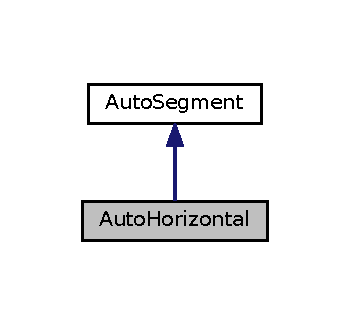
\includegraphics[width=168pt]{classKatabatic_1_1AutoHorizontal__inherit__graph}
\end{center}
\end{figure}
\subsection*{Public Member Functions}
\begin{DoxyCompactItemize}
\item 
virtual bool \mbox{\hyperlink{classKatabatic_1_1AutoHorizontal_a2ced98fb06f208aa88c0962a706e64db}{\+\_\+can\+Slacken}} () const
\item 
virtual bool \mbox{\hyperlink{classKatabatic_1_1AutoHorizontal_a9b0c21eeb26c256876592ba63438da74}{can\+Move\+U\+Left}} (float reserve=0.\+0) const
\item 
virtual bool \mbox{\hyperlink{classKatabatic_1_1AutoHorizontal_ad0c972e34d6bac47bd9276a7d6e053d8}{can\+Move\+U\+Right}} (float reserve=0.\+0) const
\item 
virtual \textbf{ Segment} $\ast$ \mbox{\hyperlink{classKatabatic_1_1AutoHorizontal_a9e651c17b47f82166a02865c9296a2df}{base}} ()
\item 
virtual \textbf{ Segment} $\ast$ \mbox{\hyperlink{classKatabatic_1_1AutoHorizontal_a6f14a3faa93f2c610ea0d2cc7d903706}{base}} () const
\item 
virtual \textbf{ Horizontal} $\ast$ \mbox{\hyperlink{classKatabatic_1_1AutoHorizontal_a659b8ed90de679564924afe07af478de}{get\+Horizontal}} ()
\item 
virtual \textbf{ Db\+U\+::\+Unit} \mbox{\hyperlink{classKatabatic_1_1AutoHorizontal_ad521ffba761b0e81b7b81b99d62f76f9}{get\+SourceU}} () const
\item 
virtual \textbf{ Db\+U\+::\+Unit} \mbox{\hyperlink{classKatabatic_1_1AutoHorizontal_a4d52a506cd19dfa8e22e1dc0695bd960}{get\+TargetU}} () const
\item 
virtual \textbf{ Db\+U\+::\+Unit} \mbox{\hyperlink{classKatabatic_1_1AutoHorizontal_a760500b1fd027c71f5362dd8c0b01ea7}{get\+Du\+Source}} () const
\item 
virtual \textbf{ Db\+U\+::\+Unit} \mbox{\hyperlink{classKatabatic_1_1AutoHorizontal_a76e349c14c904b3300a15caa1ee8b680}{get\+Du\+Target}} () const
\item 
virtual \textbf{ Interval} \mbox{\hyperlink{classKatabatic_1_1AutoHorizontal_a0b5ac47ab175815e1a9bc07f2517614a}{get\+SpanU}} () const
\item 
virtual bool \mbox{\hyperlink{classKatabatic_1_1AutoHorizontal_a16737e7f2b77f8595fd2b607fac0f2f5}{get\+Constraints}} (\textbf{ Db\+U\+::\+Unit} \&min, \textbf{ Db\+U\+::\+Unit} \&max) const
\item 
virtual \textbf{ Interval} \mbox{\hyperlink{classKatabatic_1_1AutoHorizontal_a3239751f475bc65adb9d56f6c771ebb0}{get\+Source\+Constraints}} (unsigned int flags=0) const
\item 
virtual \textbf{ Interval} \mbox{\hyperlink{classKatabatic_1_1AutoHorizontal_ad2b5aeb2604548378c8d78c60862091f}{get\+Target\+Constraints}} (unsigned int flags=0) const
\item 
virtual unsigned int \mbox{\hyperlink{classKatabatic_1_1AutoHorizontal_a0dd7cf705ace42c662c289955313b2e9}{get\+Direction}} () const
\item 
virtual size\+\_\+t \mbox{\hyperlink{classKatabatic_1_1AutoHorizontal_accdaef4410043f64da247a94a309733e}{get\+G\+Cells}} (vector$<$ \mbox{\hyperlink{classKatabatic_1_1GCell}{G\+Cell}} $\ast$$>$ \&) const
\item 
virtual void \mbox{\hyperlink{classKatabatic_1_1AutoHorizontal_a756616a1967c5ad8efd08be96d18f25d}{set\+Du\+Source}} (\textbf{ Db\+U\+::\+Unit})
\item 
virtual void \mbox{\hyperlink{classKatabatic_1_1AutoHorizontal_a9df2ef68c1fbf4159cc837be5c699b53}{set\+Du\+Target}} (\textbf{ Db\+U\+::\+Unit})
\item 
virtual void \mbox{\hyperlink{classKatabatic_1_1AutoHorizontal_a59058f4593049c583c5b3698ff81b299}{update\+Orient}} ()
\item 
virtual void \mbox{\hyperlink{classKatabatic_1_1AutoHorizontal_a9662a77c2ed8553d6a0312c5292060ad}{update\+Positions}} ()
\item 
virtual bool \mbox{\hyperlink{classKatabatic_1_1AutoHorizontal_a6575c17bfa589c087215c87678e5719c}{check\+Positions}} () const
\item 
virtual bool \mbox{\hyperlink{classKatabatic_1_1AutoHorizontal_a8aef8f4bbafe3426840f9ebf31bb3b81}{check\+Constraints}} () const
\item 
virtual unsigned int \mbox{\hyperlink{classKatabatic_1_1AutoHorizontal_a36c0eecad40d3559b5378caefec6a7e0}{\+\_\+make\+Dogleg}} (\mbox{\hyperlink{classKatabatic_1_1GCell}{G\+Cell}} $\ast$, unsigned int flags)
\item 
virtual bool \mbox{\hyperlink{classKatabatic_1_1AutoHorizontal_a1fa2421b74bf0eb934b7002fd3da2321}{move\+U\+Left}} ()
\item 
virtual bool \mbox{\hyperlink{classKatabatic_1_1AutoHorizontal_aa469e37853e31f8b1bc817518c896d62}{move\+U\+Right}} ()
\end{DoxyCompactItemize}
\subsection*{Protected Member Functions}
\begin{DoxyCompactItemize}
\item 
virtual void \mbox{\hyperlink{classKatabatic_1_1AutoHorizontal_a3715b38135ca24745f610bebd3407c10}{\+\_\+post\+Create}} ()
\item 
virtual void \mbox{\hyperlink{classKatabatic_1_1AutoHorizontal_a7c13d9795eafd477994961f8a0d962d0}{\+\_\+pre\+Destroy}} ()
\end{DoxyCompactItemize}
\subsection*{Additional Inherited Members}


\subsection{Detailed Description}
Concrete Horizontal \mbox{\hyperlink{classKatabatic_1_1AutoSegment}{Auto\+Segment}}. 

\subsection{Member Function Documentation}
\mbox{\Hypertarget{classKatabatic_1_1AutoHorizontal_a2ced98fb06f208aa88c0962a706e64db}\label{classKatabatic_1_1AutoHorizontal_a2ced98fb06f208aa88c0962a706e64db}} 
\index{Katabatic\+::\+Auto\+Horizontal@{Katabatic\+::\+Auto\+Horizontal}!\+\_\+can\+Slacken@{\+\_\+can\+Slacken}}
\index{\+\_\+can\+Slacken@{\+\_\+can\+Slacken}!Katabatic\+::\+Auto\+Horizontal@{Katabatic\+::\+Auto\+Horizontal}}
\subsubsection{\texorpdfstring{\+\_\+can\+Slacken()}{\_canSlacken()}}
{\footnotesize\ttfamily bool \+\_\+can\+Slacken (\begin{DoxyParamCaption}{ }\end{DoxyParamCaption}) const\hspace{0.3cm}{\ttfamily [virtual]}}

{\bfseries Returns\+:} {\bfseries true} if the segment can be slackened. That is, source or target constraints are less than three pitches. 

Implements \mbox{\hyperlink{classKatabatic_1_1AutoSegment_a676fcb7ece71d129b7a4d87a3f2e07aa}{Auto\+Segment}}.



References Interval\+::contains(), Auto\+Segment\+::get\+Auto\+Source(), Auto\+Segment\+::get\+Auto\+Target(), Auto\+Contact\+::get\+G\+Cell(), G\+Cell\+::get\+Side(), Interval\+::get\+Size(), Db\+U\+::get\+Value\+String(), Interval\+::inflate(), and Katabatic\+::\+Kb\+Vertical.

\mbox{\Hypertarget{classKatabatic_1_1AutoHorizontal_a9b0c21eeb26c256876592ba63438da74}\label{classKatabatic_1_1AutoHorizontal_a9b0c21eeb26c256876592ba63438da74}} 
\index{Katabatic\+::\+Auto\+Horizontal@{Katabatic\+::\+Auto\+Horizontal}!can\+Move\+U\+Left@{can\+Move\+U\+Left}}
\index{can\+Move\+U\+Left@{can\+Move\+U\+Left}!Katabatic\+::\+Auto\+Horizontal@{Katabatic\+::\+Auto\+Horizontal}}
\subsubsection{\texorpdfstring{can\+Move\+U\+Left()}{canMoveULeft()}}
{\footnotesize\ttfamily bool can\+Move\+U\+Left (\begin{DoxyParamCaption}\item[{float}]{reserve = {\ttfamily 0.0} }\end{DoxyParamCaption}) const\hspace{0.3cm}{\ttfamily [virtual]}}

\begin{DoxyReturn}{Returns}
{\bfseries true} if the {\itshape global} segment can be moved on the left \mbox{\hyperlink{classKatabatic_1_1GCell}{G\+Cell}} (for a vertical) or down (for an horizontal). The move is accepted only if it do not change the amount of global wiring. Thus the following conditions\+:
\begin{DoxyItemize}
\item The segment mustn\textquotesingle{}t be on the leftmost \mbox{\hyperlink{classKatabatic_1_1GCell}{G\+Cell}} (obvious...).
\item The segment must be global.
\item The source and target contacts must be Auto\+Contact\+Turn(s).
\item At least one of the perpandicular must be global {\bfseries and} connected through the {\itshape target}. That is, it\textquotesingle{}s a global which extends toward left.
\item The \mbox{\hyperlink{classKatabatic_1_1GCell}{G\+Cell}} of maximum density on the left must remains below the current \mbox{\hyperlink{classKatabatic_1_1GCell}{G\+Cell}} of maximum density, with a margin of {\ttfamily reserve} (expressed in total saturation percentage). 
\end{DoxyItemize}
\end{DoxyReturn}


Implements \mbox{\hyperlink{classKatabatic_1_1AutoSegment_aad55626c9d793a0b08bcff5be2a5ad0c}{Auto\+Segment}}.



References Auto\+Segment\+::get\+Auto\+Source(), Auto\+Segment\+::get\+Auto\+Target(), G\+Cell\+::get\+Down(), Auto\+Contact\+::get\+G\+Cell(), Auto\+Segment\+::get\+G\+Cell(), Auto\+Segment\+::get\+Layer(), Routing\+Gauge\+::get\+Layer\+Depth(), G\+Cell\+::get\+Right(), Session\+::get\+Routing\+Gauge(), Auto\+Contact\+::get\+Segment(), G\+Cell\+::get\+W\+Density(), and Auto\+Segment\+::is\+Global().

\mbox{\Hypertarget{classKatabatic_1_1AutoHorizontal_ad0c972e34d6bac47bd9276a7d6e053d8}\label{classKatabatic_1_1AutoHorizontal_ad0c972e34d6bac47bd9276a7d6e053d8}} 
\index{Katabatic\+::\+Auto\+Horizontal@{Katabatic\+::\+Auto\+Horizontal}!can\+Move\+U\+Right@{can\+Move\+U\+Right}}
\index{can\+Move\+U\+Right@{can\+Move\+U\+Right}!Katabatic\+::\+Auto\+Horizontal@{Katabatic\+::\+Auto\+Horizontal}}
\subsubsection{\texorpdfstring{can\+Move\+U\+Right()}{canMoveURight()}}
{\footnotesize\ttfamily bool can\+Move\+U\+Right (\begin{DoxyParamCaption}\item[{float}]{reserve = {\ttfamily 0.0} }\end{DoxyParamCaption}) const\hspace{0.3cm}{\ttfamily [virtual]}}

\begin{DoxyReturn}{Returns}
{\bfseries true} if the {\itshape global} segment can be moved on the right \mbox{\hyperlink{classKatabatic_1_1GCell}{G\+Cell}} (for a vertical) or up (for an horizontal). The move is accepted only if it do not change the amount of global wiring. Thus the following conditions\+:
\begin{DoxyItemize}
\item The segment mustn\textquotesingle{}t be on the leftmost \mbox{\hyperlink{classKatabatic_1_1GCell}{G\+Cell}} (obvious...).
\item The segment must be global.
\item The source and target contacts must be Auto\+Contact\+Turn(s).
\item At least one of the perpandicular must be global {\bfseries and} connected through the {\itshape source}. That is, it\textquotesingle{}s a global which extends toward right.
\item The \mbox{\hyperlink{classKatabatic_1_1GCell}{G\+Cell}} of maximum density on the left must remains below the current \mbox{\hyperlink{classKatabatic_1_1GCell}{G\+Cell}} of maximum density, with a margin of {\ttfamily reserve} (expressed in total saturation percentage). 
\end{DoxyItemize}
\end{DoxyReturn}


Implements \mbox{\hyperlink{classKatabatic_1_1AutoSegment_a096deb8a143f098eac2bff9ab9c52243}{Auto\+Segment}}.



References Auto\+Segment\+::get\+Auto\+Source(), Auto\+Segment\+::get\+Auto\+Target(), Auto\+Contact\+::get\+G\+Cell(), Auto\+Segment\+::get\+G\+Cell(), Auto\+Segment\+::get\+Layer(), Routing\+Gauge\+::get\+Layer\+Depth(), G\+Cell\+::get\+Right(), Session\+::get\+Routing\+Gauge(), Auto\+Contact\+::get\+Segment(), G\+Cell\+::get\+Up(), G\+Cell\+::get\+W\+Density(), and Auto\+Segment\+::is\+Global().

\mbox{\Hypertarget{classKatabatic_1_1AutoHorizontal_a9e651c17b47f82166a02865c9296a2df}\label{classKatabatic_1_1AutoHorizontal_a9e651c17b47f82166a02865c9296a2df}} 
\index{Katabatic\+::\+Auto\+Horizontal@{Katabatic\+::\+Auto\+Horizontal}!base@{base}}
\index{base@{base}!Katabatic\+::\+Auto\+Horizontal@{Katabatic\+::\+Auto\+Horizontal}}
\subsubsection{\texorpdfstring{base()}{base()}\hspace{0.1cm}{\footnotesize\ttfamily [1/2]}}
{\footnotesize\ttfamily \textbf{ Segment} $\ast$ base (\begin{DoxyParamCaption}{ }\end{DoxyParamCaption})\hspace{0.3cm}{\ttfamily [virtual]}}

{\bfseries Returns\+:} the decorated \textbf{ Hurricane\+::\+Segment}. 

Implements \mbox{\hyperlink{classKatabatic_1_1AutoSegment_ade416d0483aefe986988fa89a7cf6fcf}{Auto\+Segment}}.

\mbox{\Hypertarget{classKatabatic_1_1AutoHorizontal_a6f14a3faa93f2c610ea0d2cc7d903706}\label{classKatabatic_1_1AutoHorizontal_a6f14a3faa93f2c610ea0d2cc7d903706}} 
\index{Katabatic\+::\+Auto\+Horizontal@{Katabatic\+::\+Auto\+Horizontal}!base@{base}}
\index{base@{base}!Katabatic\+::\+Auto\+Horizontal@{Katabatic\+::\+Auto\+Horizontal}}
\subsubsection{\texorpdfstring{base()}{base()}\hspace{0.1cm}{\footnotesize\ttfamily [2/2]}}
{\footnotesize\ttfamily \textbf{ Segment} $\ast$ base (\begin{DoxyParamCaption}{ }\end{DoxyParamCaption}) const\hspace{0.3cm}{\ttfamily [virtual]}}

{\bfseries Returns\+:} the decorated \textbf{ Hurricane\+::\+Segment} (const flavor). 

Implements \mbox{\hyperlink{classKatabatic_1_1AutoSegment_a53877ff5ef48eb0030c2581a6eeb3c09}{Auto\+Segment}}.

\mbox{\Hypertarget{classKatabatic_1_1AutoHorizontal_a659b8ed90de679564924afe07af478de}\label{classKatabatic_1_1AutoHorizontal_a659b8ed90de679564924afe07af478de}} 
\index{Katabatic\+::\+Auto\+Horizontal@{Katabatic\+::\+Auto\+Horizontal}!get\+Horizontal@{get\+Horizontal}}
\index{get\+Horizontal@{get\+Horizontal}!Katabatic\+::\+Auto\+Horizontal@{Katabatic\+::\+Auto\+Horizontal}}
\subsubsection{\texorpdfstring{get\+Horizontal()}{getHorizontal()}}
{\footnotesize\ttfamily \textbf{ Horizontal} $\ast$ get\+Horizontal (\begin{DoxyParamCaption}{ }\end{DoxyParamCaption})\hspace{0.3cm}{\ttfamily [virtual]}}

{\bfseries Returns\+:} If the decorated segment is a \textbf{ Hurricane\+::\+Horizontal}, return it. {\ttfamily N\+U\+LL} otherwise. 

Reimplemented from \mbox{\hyperlink{classKatabatic_1_1AutoSegment_a659b8ed90de679564924afe07af478de}{Auto\+Segment}}.

\mbox{\Hypertarget{classKatabatic_1_1AutoHorizontal_ad521ffba761b0e81b7b81b99d62f76f9}\label{classKatabatic_1_1AutoHorizontal_ad521ffba761b0e81b7b81b99d62f76f9}} 
\index{Katabatic\+::\+Auto\+Horizontal@{Katabatic\+::\+Auto\+Horizontal}!get\+SourceU@{get\+SourceU}}
\index{get\+SourceU@{get\+SourceU}!Katabatic\+::\+Auto\+Horizontal@{Katabatic\+::\+Auto\+Horizontal}}
\subsubsection{\texorpdfstring{get\+Source\+U()}{getSourceU()}}
{\footnotesize\ttfamily \textbf{ Db\+U\+::\+Unit} get\+SourceU (\begin{DoxyParamCaption}{ }\end{DoxyParamCaption}) const\hspace{0.3cm}{\ttfamily [virtual]}}

{\bfseries Returns\+:} The \mbox{\hyperlink{classKatabatic_1_1AutoSegment}{Auto\+Segment}} {\itshape uniform} source position. (X for an horizontal and Y for a Vertical). 

Implements \mbox{\hyperlink{classKatabatic_1_1AutoSegment_aeaa1543880686755e389c4807128428f}{Auto\+Segment}}.



References Segment\+::get\+Source\+X().

\mbox{\Hypertarget{classKatabatic_1_1AutoHorizontal_a4d52a506cd19dfa8e22e1dc0695bd960}\label{classKatabatic_1_1AutoHorizontal_a4d52a506cd19dfa8e22e1dc0695bd960}} 
\index{Katabatic\+::\+Auto\+Horizontal@{Katabatic\+::\+Auto\+Horizontal}!get\+TargetU@{get\+TargetU}}
\index{get\+TargetU@{get\+TargetU}!Katabatic\+::\+Auto\+Horizontal@{Katabatic\+::\+Auto\+Horizontal}}
\subsubsection{\texorpdfstring{get\+Target\+U()}{getTargetU()}}
{\footnotesize\ttfamily \textbf{ Db\+U\+::\+Unit} get\+TargetU (\begin{DoxyParamCaption}{ }\end{DoxyParamCaption}) const\hspace{0.3cm}{\ttfamily [virtual]}}

{\bfseries Returns\+:} The \mbox{\hyperlink{classKatabatic_1_1AutoSegment}{Auto\+Segment}} {\itshape uniform} target position. (X for an horizontal and Y for a Vertical). 

Implements \mbox{\hyperlink{classKatabatic_1_1AutoSegment_a828fef2716cc9c370d6d170bb96556ec}{Auto\+Segment}}.



References Segment\+::get\+Target\+X().

\mbox{\Hypertarget{classKatabatic_1_1AutoHorizontal_a760500b1fd027c71f5362dd8c0b01ea7}\label{classKatabatic_1_1AutoHorizontal_a760500b1fd027c71f5362dd8c0b01ea7}} 
\index{Katabatic\+::\+Auto\+Horizontal@{Katabatic\+::\+Auto\+Horizontal}!get\+Du\+Source@{get\+Du\+Source}}
\index{get\+Du\+Source@{get\+Du\+Source}!Katabatic\+::\+Auto\+Horizontal@{Katabatic\+::\+Auto\+Horizontal}}
\subsubsection{\texorpdfstring{get\+Du\+Source()}{getDuSource()}}
{\footnotesize\ttfamily \textbf{ Db\+U\+::\+Unit} get\+Du\+Source (\begin{DoxyParamCaption}{ }\end{DoxyParamCaption}) const\hspace{0.3cm}{\ttfamily [virtual]}}

{\bfseries Returns\+:} The \mbox{\hyperlink{classKatabatic_1_1AutoSegment}{Auto\+Segment}} {\itshape uniform} delta from source. (dX for an horizontal and dY for a Vertical). 

Implements \mbox{\hyperlink{classKatabatic_1_1AutoSegment_ab4881df67bd8f036d0199ed6540fe774}{Auto\+Segment}}.



References Horizontal\+::get\+Dx\+Source().

\mbox{\Hypertarget{classKatabatic_1_1AutoHorizontal_a76e349c14c904b3300a15caa1ee8b680}\label{classKatabatic_1_1AutoHorizontal_a76e349c14c904b3300a15caa1ee8b680}} 
\index{Katabatic\+::\+Auto\+Horizontal@{Katabatic\+::\+Auto\+Horizontal}!get\+Du\+Target@{get\+Du\+Target}}
\index{get\+Du\+Target@{get\+Du\+Target}!Katabatic\+::\+Auto\+Horizontal@{Katabatic\+::\+Auto\+Horizontal}}
\subsubsection{\texorpdfstring{get\+Du\+Target()}{getDuTarget()}}
{\footnotesize\ttfamily \textbf{ Db\+U\+::\+Unit} get\+Du\+Target (\begin{DoxyParamCaption}{ }\end{DoxyParamCaption}) const\hspace{0.3cm}{\ttfamily [virtual]}}

{\bfseries Returns\+:} The \mbox{\hyperlink{classKatabatic_1_1AutoSegment}{Auto\+Segment}} {\itshape uniform} delta from source. (dX for an horizontal and dY for a Vertical). 

Implements \mbox{\hyperlink{classKatabatic_1_1AutoSegment_a0644d656eedc71dba2fb3c6c0d83ed3f}{Auto\+Segment}}.



References Horizontal\+::get\+Dx\+Target().

\mbox{\Hypertarget{classKatabatic_1_1AutoHorizontal_a0b5ac47ab175815e1a9bc07f2517614a}\label{classKatabatic_1_1AutoHorizontal_a0b5ac47ab175815e1a9bc07f2517614a}} 
\index{Katabatic\+::\+Auto\+Horizontal@{Katabatic\+::\+Auto\+Horizontal}!get\+SpanU@{get\+SpanU}}
\index{get\+SpanU@{get\+SpanU}!Katabatic\+::\+Auto\+Horizontal@{Katabatic\+::\+Auto\+Horizontal}}
\subsubsection{\texorpdfstring{get\+Span\+U()}{getSpanU()}}
{\footnotesize\ttfamily \textbf{ Interval} get\+SpanU (\begin{DoxyParamCaption}{ }\end{DoxyParamCaption}) const\hspace{0.3cm}{\ttfamily [virtual]}}

{\bfseries Returns\+:} The \mbox{\hyperlink{classKatabatic_1_1AutoSegment}{Auto\+Segment}} {\itshape uniform} occupying interval (on X for horizontal and on Y for vertical). 

Implements \mbox{\hyperlink{classKatabatic_1_1AutoSegment_a248eb2fbb06e3286650b28567d495f0b}{Auto\+Segment}}.



References Segment\+::get\+Source\+X(), and Segment\+::get\+Target\+X().

\mbox{\Hypertarget{classKatabatic_1_1AutoHorizontal_a16737e7f2b77f8595fd2b607fac0f2f5}\label{classKatabatic_1_1AutoHorizontal_a16737e7f2b77f8595fd2b607fac0f2f5}} 
\index{Katabatic\+::\+Auto\+Horizontal@{Katabatic\+::\+Auto\+Horizontal}!get\+Constraints@{get\+Constraints}}
\index{get\+Constraints@{get\+Constraints}!Katabatic\+::\+Auto\+Horizontal@{Katabatic\+::\+Auto\+Horizontal}}
\subsubsection{\texorpdfstring{get\+Constraints()}{getConstraints()}}
{\footnotesize\ttfamily bool get\+Constraints (\begin{DoxyParamCaption}\item[{\textbf{ Db\+U\+::\+Unit} \&}]{min,  }\item[{\textbf{ Db\+U\+::\+Unit} \&}]{max }\end{DoxyParamCaption}) const\hspace{0.3cm}{\ttfamily [virtual]}}

{\bfseries Returns\+:} in {\ttfamily min} \& {\ttfamily max} the allowed range for the segment axis. 

Implements \mbox{\hyperlink{classKatabatic_1_1AutoSegment_a7c2fed22b081f8d3b7a69abb457153ea}{Auto\+Segment}}.



References Auto\+Segment\+::get\+Auto\+Source(), Auto\+Segment\+::get\+Auto\+Target(), Auto\+Contact\+::get\+C\+B\+Y\+Max(), Auto\+Contact\+::get\+C\+B\+Y\+Min(), Auto\+Segment\+::get\+User\+Constraints(), and Db\+U\+::get\+Value\+String().

\mbox{\Hypertarget{classKatabatic_1_1AutoHorizontal_a3239751f475bc65adb9d56f6c771ebb0}\label{classKatabatic_1_1AutoHorizontal_a3239751f475bc65adb9d56f6c771ebb0}} 
\index{Katabatic\+::\+Auto\+Horizontal@{Katabatic\+::\+Auto\+Horizontal}!get\+Source\+Constraints@{get\+Source\+Constraints}}
\index{get\+Source\+Constraints@{get\+Source\+Constraints}!Katabatic\+::\+Auto\+Horizontal@{Katabatic\+::\+Auto\+Horizontal}}
\subsubsection{\texorpdfstring{get\+Source\+Constraints()}{getSourceConstraints()}}
{\footnotesize\ttfamily \textbf{ Interval} get\+Source\+Constraints (\begin{DoxyParamCaption}\item[{unsigned int}]{flags = {\ttfamily 0} }\end{DoxyParamCaption}) const\hspace{0.3cm}{\ttfamily [virtual]}}

\begin{DoxyReturn}{Returns}
The Interval into witch the source \mbox{\hyperlink{classKatabatic_1_1AutoContact}{Auto\+Contact}} can vary. By default all deduced constraints and user constraints are took into account. If {\ttfamily flags} contains {\ttfamily Kb\+Native\+Constraints} the constraint returned is only the enclosing \mbox{\hyperlink{classKatabatic_1_1GCell}{G\+Cell}}. 
\end{DoxyReturn}


Implements \mbox{\hyperlink{classKatabatic_1_1AutoSegment_ab7685e309e1d910db3e8237f8a898c35}{Auto\+Segment}}.



References Auto\+Segment\+::get\+Auto\+Source(), Box\+::get\+Y\+Max(), Box\+::get\+Y\+Min(), and Katabatic\+::\+Kb\+Native\+Constraints.

\mbox{\Hypertarget{classKatabatic_1_1AutoHorizontal_ad2b5aeb2604548378c8d78c60862091f}\label{classKatabatic_1_1AutoHorizontal_ad2b5aeb2604548378c8d78c60862091f}} 
\index{Katabatic\+::\+Auto\+Horizontal@{Katabatic\+::\+Auto\+Horizontal}!get\+Target\+Constraints@{get\+Target\+Constraints}}
\index{get\+Target\+Constraints@{get\+Target\+Constraints}!Katabatic\+::\+Auto\+Horizontal@{Katabatic\+::\+Auto\+Horizontal}}
\subsubsection{\texorpdfstring{get\+Target\+Constraints()}{getTargetConstraints()}}
{\footnotesize\ttfamily \textbf{ Interval} get\+Target\+Constraints (\begin{DoxyParamCaption}\item[{unsigned int}]{flags = {\ttfamily 0} }\end{DoxyParamCaption}) const\hspace{0.3cm}{\ttfamily [virtual]}}

\begin{DoxyReturn}{Returns}
The Interval into witch the target \mbox{\hyperlink{classKatabatic_1_1AutoContact}{Auto\+Contact}} can vary. By default all deduced constraints and user constraints are took into account. If {\ttfamily flags} contains {\ttfamily Kb\+Native\+Constraints} the constraint returned is only the enclosing \mbox{\hyperlink{classKatabatic_1_1GCell}{G\+Cell}}. 
\end{DoxyReturn}


Implements \mbox{\hyperlink{classKatabatic_1_1AutoSegment_a9c1b8b3cd57fb7b0bf60c7a6148237c2}{Auto\+Segment}}.



References Auto\+Segment\+::get\+Auto\+Target(), Box\+::get\+Y\+Max(), Box\+::get\+Y\+Min(), and Katabatic\+::\+Kb\+Native\+Constraints.

\mbox{\Hypertarget{classKatabatic_1_1AutoHorizontal_a0dd7cf705ace42c662c289955313b2e9}\label{classKatabatic_1_1AutoHorizontal_a0dd7cf705ace42c662c289955313b2e9}} 
\index{Katabatic\+::\+Auto\+Horizontal@{Katabatic\+::\+Auto\+Horizontal}!get\+Direction@{get\+Direction}}
\index{get\+Direction@{get\+Direction}!Katabatic\+::\+Auto\+Horizontal@{Katabatic\+::\+Auto\+Horizontal}}
\subsubsection{\texorpdfstring{get\+Direction()}{getDirection()}}
{\footnotesize\ttfamily unsigned int get\+Direction (\begin{DoxyParamCaption}{ }\end{DoxyParamCaption}) const\hspace{0.3cm}{\ttfamily [virtual]}}

{\bfseries Returns\+:} \mbox{\hyperlink{namespaceKatabatic_a2af2ad6b6441614038caf59d04b3b217a1a9045673c5d3c30b067100f1440ae1b}{Katabatic\+::\+Kb\+Horizontal}} or \mbox{\hyperlink{namespaceKatabatic_a2af2ad6b6441614038caf59d04b3b217a284cad95203a27172838b09e396e3590}{Katabatic\+::\+Kb\+Vertical}} according to the decorated segment. 

Implements \mbox{\hyperlink{classKatabatic_1_1AutoSegment_ae35b78590ed6aa546b626ef95f28c533}{Auto\+Segment}}.



References Katabatic\+::\+Kb\+Horizontal.

\mbox{\Hypertarget{classKatabatic_1_1AutoHorizontal_accdaef4410043f64da247a94a309733e}\label{classKatabatic_1_1AutoHorizontal_accdaef4410043f64da247a94a309733e}} 
\index{Katabatic\+::\+Auto\+Horizontal@{Katabatic\+::\+Auto\+Horizontal}!get\+G\+Cells@{get\+G\+Cells}}
\index{get\+G\+Cells@{get\+G\+Cells}!Katabatic\+::\+Auto\+Horizontal@{Katabatic\+::\+Auto\+Horizontal}}
\subsubsection{\texorpdfstring{get\+G\+Cells()}{getGCells()}}
{\footnotesize\ttfamily size\+\_\+t get\+G\+Cells (\begin{DoxyParamCaption}\item[{vector$<$ \mbox{\hyperlink{classKatabatic_1_1GCell}{G\+Cell}} $\ast$$>$ \&}]{gcells }\end{DoxyParamCaption}) const\hspace{0.3cm}{\ttfamily [virtual]}}


\begin{DoxyParams}{Parameters}
{\em gcells} & A vector that will be filled by all the G\+Cells that the segment overlap. In increasing order, from source to target. \\
\hline
\end{DoxyParams}
\begin{DoxyReturn}{Returns}
The vector\textquotesingle{}s size. 
\end{DoxyReturn}


Implements \mbox{\hyperlink{classKatabatic_1_1AutoSegment_a8ca0022e253d355817d46a057ae01625}{Auto\+Segment}}.



References Auto\+Segment\+::get\+Auto\+Source(), Auto\+Segment\+::get\+Auto\+Target(), Auto\+Contact\+::get\+G\+Cell(), Auto\+Segment\+::get\+G\+Cell(), and G\+Cell\+::get\+Right().

\mbox{\Hypertarget{classKatabatic_1_1AutoHorizontal_a756616a1967c5ad8efd08be96d18f25d}\label{classKatabatic_1_1AutoHorizontal_a756616a1967c5ad8efd08be96d18f25d}} 
\index{Katabatic\+::\+Auto\+Horizontal@{Katabatic\+::\+Auto\+Horizontal}!set\+Du\+Source@{set\+Du\+Source}}
\index{set\+Du\+Source@{set\+Du\+Source}!Katabatic\+::\+Auto\+Horizontal@{Katabatic\+::\+Auto\+Horizontal}}
\subsubsection{\texorpdfstring{set\+Du\+Source()}{setDuSource()}}
{\footnotesize\ttfamily void set\+Du\+Source (\begin{DoxyParamCaption}\item[{\textbf{ Db\+U\+::\+Unit}}]{du }\end{DoxyParamCaption})\hspace{0.3cm}{\ttfamily [virtual]}}

Set the {\itshape uniform} {\ttfamily dU} from source anchor (dX for Horizontal, dY for Vertical). 

Implements \mbox{\hyperlink{classKatabatic_1_1AutoSegment_aaf60d18ab6d951a34a3d06959ce2e76f}{Auto\+Segment}}.

\mbox{\Hypertarget{classKatabatic_1_1AutoHorizontal_a9df2ef68c1fbf4159cc837be5c699b53}\label{classKatabatic_1_1AutoHorizontal_a9df2ef68c1fbf4159cc837be5c699b53}} 
\index{Katabatic\+::\+Auto\+Horizontal@{Katabatic\+::\+Auto\+Horizontal}!set\+Du\+Target@{set\+Du\+Target}}
\index{set\+Du\+Target@{set\+Du\+Target}!Katabatic\+::\+Auto\+Horizontal@{Katabatic\+::\+Auto\+Horizontal}}
\subsubsection{\texorpdfstring{set\+Du\+Target()}{setDuTarget()}}
{\footnotesize\ttfamily void set\+Du\+Target (\begin{DoxyParamCaption}\item[{\textbf{ Db\+U\+::\+Unit}}]{du }\end{DoxyParamCaption})\hspace{0.3cm}{\ttfamily [virtual]}}

Set the {\itshape uniform} {\ttfamily dU} from target anchor (dX for Horizontal, dY for Vertical). 

Implements \mbox{\hyperlink{classKatabatic_1_1AutoSegment_a246756d4c8b3e094a0a9d6de3c2109ff}{Auto\+Segment}}.

\mbox{\Hypertarget{classKatabatic_1_1AutoHorizontal_a59058f4593049c583c5b3698ff81b299}\label{classKatabatic_1_1AutoHorizontal_a59058f4593049c583c5b3698ff81b299}} 
\index{Katabatic\+::\+Auto\+Horizontal@{Katabatic\+::\+Auto\+Horizontal}!update\+Orient@{update\+Orient}}
\index{update\+Orient@{update\+Orient}!Katabatic\+::\+Auto\+Horizontal@{Katabatic\+::\+Auto\+Horizontal}}
\subsubsection{\texorpdfstring{update\+Orient()}{updateOrient()}}
{\footnotesize\ttfamily void update\+Orient (\begin{DoxyParamCaption}{ }\end{DoxyParamCaption})\hspace{0.3cm}{\ttfamily [virtual]}}

Ensure that source is lower than target. Swap them if needed. Swap never occurs on global segment because their source and target anchors are from different \mbox{\hyperlink{classKatabatic_1_1GCell}{G\+Cell}}, which are already ordered. 

Implements \mbox{\hyperlink{classKatabatic_1_1AutoSegment_a102e0f4bbb0386e41be214d15a9e4549}{Auto\+Segment}}.



References Segment\+::get\+Source\+X(), Segment\+::get\+Target\+X(), Segment\+::invert(), Katabatic\+::\+Seg\+Source\+Bottom, Katabatic\+::\+Seg\+Source\+Top, Katabatic\+::\+Seg\+Strong\+Terminal, Katabatic\+::\+Seg\+Target\+Bottom, Katabatic\+::\+Seg\+Target\+Top, Auto\+Segment\+::set\+Flags(), and Auto\+Segment\+::unset\+Flags().

\mbox{\Hypertarget{classKatabatic_1_1AutoHorizontal_a9662a77c2ed8553d6a0312c5292060ad}\label{classKatabatic_1_1AutoHorizontal_a9662a77c2ed8553d6a0312c5292060ad}} 
\index{Katabatic\+::\+Auto\+Horizontal@{Katabatic\+::\+Auto\+Horizontal}!update\+Positions@{update\+Positions}}
\index{update\+Positions@{update\+Positions}!Katabatic\+::\+Auto\+Horizontal@{Katabatic\+::\+Auto\+Horizontal}}
\subsubsection{\texorpdfstring{update\+Positions()}{updatePositions()}}
{\footnotesize\ttfamily void update\+Positions (\begin{DoxyParamCaption}{ }\end{DoxyParamCaption})\hspace{0.3cm}{\ttfamily [virtual]}}

Update the segment begenning and ending positions. The positions takes into account the extension caps and reflect the real space used by the segment under it\textquotesingle{}s long axis. 

Implements \mbox{\hyperlink{classKatabatic_1_1AutoSegment_a6d95f4de39c13611786c95ddc7b8942e}{Auto\+Segment}}.



References Session\+::get\+Extension\+Cap(), Auto\+Segment\+::get\+Layer(), Segment\+::get\+Source\+X(), and Segment\+::get\+Target\+X().

\mbox{\Hypertarget{classKatabatic_1_1AutoHorizontal_a6575c17bfa589c087215c87678e5719c}\label{classKatabatic_1_1AutoHorizontal_a6575c17bfa589c087215c87678e5719c}} 
\index{Katabatic\+::\+Auto\+Horizontal@{Katabatic\+::\+Auto\+Horizontal}!check\+Positions@{check\+Positions}}
\index{check\+Positions@{check\+Positions}!Katabatic\+::\+Auto\+Horizontal@{Katabatic\+::\+Auto\+Horizontal}}
\subsubsection{\texorpdfstring{check\+Positions()}{checkPositions()}}
{\footnotesize\ttfamily bool check\+Positions (\begin{DoxyParamCaption}{ }\end{DoxyParamCaption}) const\hspace{0.3cm}{\ttfamily [virtual]}}

{\bfseries Returns\+:} {\bfseries true} if the relative positions of source \& target are coherent. (source $<$= target). 

Implements \mbox{\hyperlink{classKatabatic_1_1AutoSegment_af026a81002bd907f1ccd4a4784aaa1db}{Auto\+Segment}}.



References Session\+::get\+Extension\+Cap(), Auto\+Segment\+::get\+Layer(), Segment\+::get\+Source\+X(), Segment\+::get\+Target\+X(), and Db\+U\+::get\+Value\+String().

\mbox{\Hypertarget{classKatabatic_1_1AutoHorizontal_a8aef8f4bbafe3426840f9ebf31bb3b81}\label{classKatabatic_1_1AutoHorizontal_a8aef8f4bbafe3426840f9ebf31bb3b81}} 
\index{Katabatic\+::\+Auto\+Horizontal@{Katabatic\+::\+Auto\+Horizontal}!check\+Constraints@{check\+Constraints}}
\index{check\+Constraints@{check\+Constraints}!Katabatic\+::\+Auto\+Horizontal@{Katabatic\+::\+Auto\+Horizontal}}
\subsubsection{\texorpdfstring{check\+Constraints()}{checkConstraints()}}
{\footnotesize\ttfamily bool check\+Constraints (\begin{DoxyParamCaption}{ }\end{DoxyParamCaption}) const\hspace{0.3cm}{\ttfamily [virtual]}}

{\bfseries Returns\+:} {\bfseries true} if the constraint intervel is coherent (non-\/empty or punctual in the worst case). 

Implements \mbox{\hyperlink{classKatabatic_1_1AutoSegment_a3d5732fd10b4a05076981066a4674487}{Auto\+Segment}}.



References Auto\+Segment\+::get\+Auto\+Source(), Auto\+Segment\+::get\+Auto\+Target(), and Interval\+::intersect().

\mbox{\Hypertarget{classKatabatic_1_1AutoHorizontal_a36c0eecad40d3559b5378caefec6a7e0}\label{classKatabatic_1_1AutoHorizontal_a36c0eecad40d3559b5378caefec6a7e0}} 
\index{Katabatic\+::\+Auto\+Horizontal@{Katabatic\+::\+Auto\+Horizontal}!\+\_\+make\+Dogleg@{\+\_\+make\+Dogleg}}
\index{\+\_\+make\+Dogleg@{\+\_\+make\+Dogleg}!Katabatic\+::\+Auto\+Horizontal@{Katabatic\+::\+Auto\+Horizontal}}
\subsubsection{\texorpdfstring{\+\_\+make\+Dogleg()}{\_makeDogleg()}}
{\footnotesize\ttfamily unsigned int \+\_\+make\+Dogleg (\begin{DoxyParamCaption}\item[{\mbox{\hyperlink{classKatabatic_1_1GCell}{G\+Cell}} $\ast$}]{dogleg\+G\+Cell,  }\item[{unsigned int}]{flags }\end{DoxyParamCaption})\hspace{0.3cm}{\ttfamily [virtual]}}

{\bfseries This method is the workhorse for the various dogleg and topology restauration methods.} It is the atomic method that actually make the dogleg on {\bfseries this} segment.

{\bfseries Returns\+:} \mbox{\hyperlink{namespaceKatabatic_a2af2ad6b6441614038caf59d04b3b217af756099f1bbe259dd1bf22067dc40eac}{Katabatic\+::\+Kb\+Use\+Above\+Layer}} if the dogleg is using the {\itshape above} layer (\mbox{\hyperlink{namespaceKatabatic_a2af2ad6b6441614038caf59d04b3b217a41cbd981337678e042354f340bfae25d}{Katabatic\+::\+Kb\+Use\+Below\+Layer}} for the below layer).

Break the current segment in two (a.\+k.\+a. making a dogleg).
\begin{DoxyItemize}
\item The segment is broken inside {\ttfamily dogleg\+G\+Cell}.
\item Two new segments are createds, one perpandicular and one parallel.
\item The original segment is always kept attached to the {\itshape source}. (the new parallel fragment is attached to the {\itshape target}).
\item The perpandicular segment is in the layer {\itshape above} by default. If we are already on the topmost routing layer, the {\itshape below} layer is used.
\item If the segment pass through the breaking \mbox{\hyperlink{classKatabatic_1_1GCell}{G\+Cell}}, it\textquotesingle{}s axis is set into the center. If the segment is local, the axis is the middle of the segment.
\item The Local/\+Global kind of the original segment is updated. The local/global status is computed by the constructor of the \mbox{\hyperlink{classKatabatic_1_1AutoSegment}{Auto\+Segment}} for the perpandicular and the new parallel.
\item The terminal state is updated. If the segment is a strong terminal the part that is no longer directly connected to the terminal is demoted to \mbox{\hyperlink{namespaceKatabatic_a94585537ee1724ea9315578ec54380f4a7b3e09b8ab4cf676fd308535d7fba892}{Katabatic\+::\+Seg\+Weak\+Terminal1}}.
\item The perpandicular is obviously a canonical. If the broken segment is canonical, the original {\bfseries is} left canonical and only the new parallel is re-\/canonized. Otherwise, we re-\/canonise both sets of aligned segments (the one on the source and the one on the target).
\item The three segments are added to the session dogleg stack.
\end{DoxyItemize}

After this method call the net topology is guarantee to be valid.

  

Implements \mbox{\hyperlink{classKatabatic_1_1AutoSegment_a37a14b40295ccb50cd5001891385807b}{Auto\+Segment}}.



References Auto\+Segment\+::canonize(), Debug\+Session\+::close(), Auto\+Contact\+Turn\+::create(), Auto\+Segment\+::create(), Session\+::dogleg(), Auto\+Segment\+::get\+Auto\+Source(), Auto\+Segment\+::get\+Auto\+Target(), Session\+::get\+Configuration(), Routing\+Gauge\+::get\+Contact\+Layer(), Auto\+Contact\+::get\+G\+Cell(), Component\+::get\+Layer(), Auto\+Segment\+::get\+Layer(), Routing\+Gauge\+::get\+Layer\+Depth(), Component\+::get\+Net(), Auto\+Segment\+::get\+Net(), G\+Cell\+::get\+Right(), Session\+::get\+Routing\+Gauge(), Routing\+Gauge\+::get\+Routing\+Layer(), Auto\+Segment\+::get\+Source\+X(), Auto\+Segment\+::get\+Target\+X(), G\+Cell\+::get\+X(), G\+Cell\+::get\+X\+Max(), Auto\+Segment\+::get\+Y(), Auto\+Contact\+::invalidate(), Auto\+Segment\+::invalidate(), Auto\+Segment\+::is\+Canonical(), Auto\+Segment\+::is\+Local(), Auto\+Segment\+::is\+Slackened(), Auto\+Segment\+::is\+Weak\+Terminal(), Katabatic\+::\+Kb\+Horizontal, Katabatic\+::\+Kb\+Use\+Above\+Layer, Katabatic\+::\+Kb\+Use\+Below\+Layer, Katabatic\+::\+Kb\+Vertical, Auto\+Contact\+::migrate\+Constraint\+Box(), Debug\+Session\+::open(), G\+Cell\+::remove\+H\+Segment(), Katabatic\+::\+Seg\+Canonical, Katabatic\+::\+Seg\+Dogleg, Katabatic\+::\+Seg\+Global, Katabatic\+::\+Seg\+Not\+Aligned, Katabatic\+::\+Seg\+Slackened, Katabatic\+::\+Seg\+Weak\+Terminal1, Auto\+Segment\+::set\+Flags(), Auto\+Segment\+::set\+Layer(), and Auto\+Segment\+::unset\+Flags().

\mbox{\Hypertarget{classKatabatic_1_1AutoHorizontal_a1fa2421b74bf0eb934b7002fd3da2321}\label{classKatabatic_1_1AutoHorizontal_a1fa2421b74bf0eb934b7002fd3da2321}} 
\index{Katabatic\+::\+Auto\+Horizontal@{Katabatic\+::\+Auto\+Horizontal}!move\+U\+Left@{move\+U\+Left}}
\index{move\+U\+Left@{move\+U\+Left}!Katabatic\+::\+Auto\+Horizontal@{Katabatic\+::\+Auto\+Horizontal}}
\subsubsection{\texorpdfstring{move\+U\+Left()}{moveULeft()}}
{\footnotesize\ttfamily bool move\+U\+Left (\begin{DoxyParamCaption}{ }\end{DoxyParamCaption})\hspace{0.3cm}{\ttfamily [virtual]}}

{\bfseries This function do not manage an aligned set. It applies on {\ttfamily this} segment only.}

Displace an Horizontal or Vertical segment to the \mbox{\hyperlink{classKatabatic_1_1GCell}{G\+Cell}} below (a.\+k.\+a. lower or inferior). Rules for displacement\+:
\begin{DoxyItemize}
\item The segment must be connected at both end to a turn contact (we do not want to manage more complex cases for the time beeing).
\item And, of course, the segment must not already by on the bottomost \mbox{\hyperlink{classKatabatic_1_1GCell}{G\+Cell}}...
\end{DoxyItemize}

The displacement take care of\+:
\begin{DoxyItemize}
\item Managing the status of the various perpandiculars. The stretched one are made global if needed. The shrinked one made local, if needed.
\item The supporting \mbox{\hyperlink{classKatabatic_1_1AutoContact}{Auto\+Contact}} (source \& target) are changed of \mbox{\hyperlink{classKatabatic_1_1GCell}{G\+Cell}}.
\item If the segment is global, the go-\/through G\+Cells are updateds.
\end{DoxyItemize}

{\bfseries Returns\+:} {\bfseries true} if the move has succeeded.

 

Implements \mbox{\hyperlink{classKatabatic_1_1AutoSegment_af8ca7b17e952f4b599aeeb2f4e5be395}{Auto\+Segment}}.



References G\+Cell\+::add\+V\+Segment(), Auto\+Segment\+::get\+Auto\+Source(), Auto\+Segment\+::get\+Auto\+Target(), G\+Cell\+::get\+Down(), Auto\+Contact\+::get\+G\+Cell(), Auto\+Segment\+::get\+G\+Cell(), G\+Cell\+::get\+Right(), Auto\+Contact\+::get\+Segment(), G\+Cell\+::get\+Side(), Interval\+::get\+V\+Max(), Auto\+Segment\+::is\+Local(), Katabatic\+::\+Kb\+Vertical, G\+Cell\+::remove\+V\+Segment(), Katabatic\+::\+Seg\+Global, Auto\+Segment\+::set\+Axis(), Auto\+Segment\+::set\+Flags(), Auto\+Contact\+::set\+G\+Cell(), and Auto\+Segment\+::unset\+Flags().

\mbox{\Hypertarget{classKatabatic_1_1AutoHorizontal_aa469e37853e31f8b1bc817518c896d62}\label{classKatabatic_1_1AutoHorizontal_aa469e37853e31f8b1bc817518c896d62}} 
\index{Katabatic\+::\+Auto\+Horizontal@{Katabatic\+::\+Auto\+Horizontal}!move\+U\+Right@{move\+U\+Right}}
\index{move\+U\+Right@{move\+U\+Right}!Katabatic\+::\+Auto\+Horizontal@{Katabatic\+::\+Auto\+Horizontal}}
\subsubsection{\texorpdfstring{move\+U\+Right()}{moveURight()}}
{\footnotesize\ttfamily bool move\+U\+Right (\begin{DoxyParamCaption}{ }\end{DoxyParamCaption})\hspace{0.3cm}{\ttfamily [virtual]}}

{\bfseries This function do not manage an aligned set. It applies on {\ttfamily this} segment only.}

Displace an Horizontal or Vertical segment to the \mbox{\hyperlink{classKatabatic_1_1GCell}{G\+Cell}} above (a.\+k.\+a. upper or superior). Rules for displacement\+:

\begin{DoxySeeAlso}{See also}
\mbox{\hyperlink{classKatabatic_1_1AutoSegment_af8ca7b17e952f4b599aeeb2f4e5be395}{Auto\+Segment\+::move\+U\+Left()}} for a complete description. 
\end{DoxySeeAlso}


Implements \mbox{\hyperlink{classKatabatic_1_1AutoSegment_ad7fd54ca229fcf5ccd99f87b019b9cbc}{Auto\+Segment}}.



References G\+Cell\+::add\+V\+Segment(), Auto\+Segment\+::get\+Auto\+Source(), Auto\+Segment\+::get\+Auto\+Target(), Auto\+Contact\+::get\+G\+Cell(), Auto\+Segment\+::get\+G\+Cell(), G\+Cell\+::get\+Right(), Auto\+Contact\+::get\+Segment(), G\+Cell\+::get\+Side(), G\+Cell\+::get\+Up(), Interval\+::get\+V\+Min(), Auto\+Segment\+::is\+Local(), Katabatic\+::\+Kb\+Vertical, G\+Cell\+::remove\+V\+Segment(), Katabatic\+::\+Seg\+Global, Auto\+Segment\+::set\+Axis(), Auto\+Segment\+::set\+Flags(), Auto\+Contact\+::set\+G\+Cell(), and Auto\+Segment\+::unset\+Flags().

\mbox{\Hypertarget{classKatabatic_1_1AutoHorizontal_a3715b38135ca24745f610bebd3407c10}\label{classKatabatic_1_1AutoHorizontal_a3715b38135ca24745f610bebd3407c10}} 
\index{Katabatic\+::\+Auto\+Horizontal@{Katabatic\+::\+Auto\+Horizontal}!\+\_\+post\+Create@{\+\_\+post\+Create}}
\index{\+\_\+post\+Create@{\+\_\+post\+Create}!Katabatic\+::\+Auto\+Horizontal@{Katabatic\+::\+Auto\+Horizontal}}
\subsubsection{\texorpdfstring{\+\_\+post\+Create()}{\_postCreate()}}
{\footnotesize\ttfamily void \+\_\+post\+Create (\begin{DoxyParamCaption}{ }\end{DoxyParamCaption})\hspace{0.3cm}{\ttfamily [protected]}, {\ttfamily [virtual]}}

In addition to \mbox{\hyperlink{classKatabatic_1_1AutoSegment_a3715b38135ca24745f610bebd3407c10}{Auto\+Segment\+::\+\_\+post\+Create()}}, detect whether the segment is global or local and register it in the relevant G\+Cells (if needed).

If the segment is anchored directly on a terminal, adjust the axis so it\textquotesingle{}s connected. 

Reimplemented from \mbox{\hyperlink{classKatabatic_1_1AutoSegment_a3715b38135ca24745f610bebd3407c10}{Auto\+Segment}}.



References Auto\+Segment\+::\+\_\+post\+Create(), G\+Cell\+::add\+H\+Segment(), Auto\+Segment\+::get\+Auto\+Source(), Auto\+Segment\+::get\+Auto\+Target(), Auto\+Contact\+::get\+G\+Cell(), G\+Cell\+::get\+Right(), G\+Cell\+::get\+X(), Component\+::get\+Y(), Katabatic\+::\+Seg\+Global, Auto\+Segment\+::set\+Flags(), and Auto\+Contact\+::set\+Y().

\mbox{\Hypertarget{classKatabatic_1_1AutoHorizontal_a7c13d9795eafd477994961f8a0d962d0}\label{classKatabatic_1_1AutoHorizontal_a7c13d9795eafd477994961f8a0d962d0}} 
\index{Katabatic\+::\+Auto\+Horizontal@{Katabatic\+::\+Auto\+Horizontal}!\+\_\+pre\+Destroy@{\+\_\+pre\+Destroy}}
\index{\+\_\+pre\+Destroy@{\+\_\+pre\+Destroy}!Katabatic\+::\+Auto\+Horizontal@{Katabatic\+::\+Auto\+Horizontal}}
\subsubsection{\texorpdfstring{\+\_\+pre\+Destroy()}{\_preDestroy()}}
{\footnotesize\ttfamily void \+\_\+pre\+Destroy (\begin{DoxyParamCaption}{ }\end{DoxyParamCaption})\hspace{0.3cm}{\ttfamily [protected]}, {\ttfamily [virtual]}}

Perform operations that must be done before the actual destructor is called. Merely whidrawn the \mbox{\hyperlink{classKatabatic_1_1AutoSegment}{Auto\+Segment}} from the lookup/\+Session mechanism. 

Reimplemented from \mbox{\hyperlink{classKatabatic_1_1AutoSegment_a7c13d9795eafd477994961f8a0d962d0}{Auto\+Segment}}.



References Auto\+Segment\+::\+\_\+pre\+Destroy(), Auto\+Segment\+::get\+Auto\+Source(), Auto\+Segment\+::get\+Auto\+Target(), Auto\+Contact\+::get\+G\+Cell(), Auto\+Segment\+::get\+Id(), G\+Cell\+::get\+Right(), G\+Cell\+::get\+X(), and G\+Cell\+::remove\+H\+Segment().



The documentation for this class was generated from the following files\+:\begin{DoxyCompactItemize}
\item 
Auto\+Horizontal.\+h\item 
Auto\+Horizontal.\+cpp\item 
Auto\+Horizontal.\+dox\end{DoxyCompactItemize}

\hypertarget{classKatabatic_1_1AutoSegment}{}\section{Auto\+Segment Class Reference}
\label{classKatabatic_1_1AutoSegment}\index{Auto\+Segment@{Auto\+Segment}}


Abstract base class for \mbox{\hyperlink{classKatabatic_1_1AutoSegment}{Auto\+Segment}}.  




Inheritance diagram for Auto\+Segment\+:\nopagebreak
\begin{figure}[H]
\begin{center}
\leavevmode
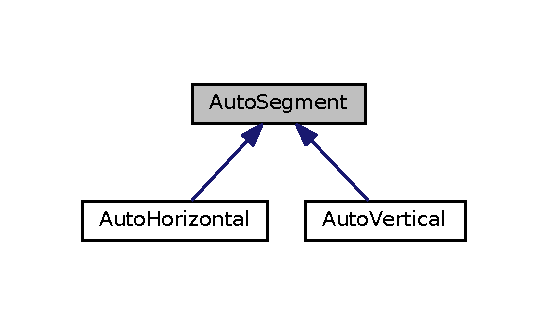
\includegraphics[width=263pt]{classKatabatic_1_1AutoSegment__inherit__graph}
\end{center}
\end{figure}
\subsection*{Public Member Functions}
\begin{DoxyCompactItemize}
\item 
virtual \textbf{ Segment} $\ast$ \mbox{\hyperlink{classKatabatic_1_1AutoSegment_a53877ff5ef48eb0030c2581a6eeb3c09}{base}} () const =0
\item 
virtual \textbf{ Segment} $\ast$ \mbox{\hyperlink{classKatabatic_1_1AutoSegment_ade416d0483aefe986988fa89a7cf6fcf}{base}} ()=0
\item 
virtual \textbf{ Horizontal} $\ast$ \mbox{\hyperlink{classKatabatic_1_1AutoSegment_a659b8ed90de679564924afe07af478de}{get\+Horizontal}} ()
\item 
virtual \textbf{ Vertical} $\ast$ \mbox{\hyperlink{classKatabatic_1_1AutoSegment_ab6a809b6f3ef3cf5385fa35580e31e7a}{get\+Vertical}} ()
\item 
\textbf{ Cell} $\ast$ \mbox{\hyperlink{classKatabatic_1_1AutoSegment_a55a3a88610ef1af9931e634f77f2403b}{get\+Cell}} () const
\item 
\textbf{ Net} $\ast$ \mbox{\hyperlink{classKatabatic_1_1AutoSegment_a692492374623a5c6096b2c4a51190359}{get\+Net}} () const
\item 
const \textbf{ Layer} $\ast$ \mbox{\hyperlink{classKatabatic_1_1AutoSegment_ab045567c4f529dca7790d66c17c3084f}{get\+Layer}} () const
\item 
\textbf{ Box} \mbox{\hyperlink{classKatabatic_1_1AutoSegment_a63a3ab1e6501bbad68b9efd4998e48c0}{get\+Bounding\+Box}} () const
\item 
\textbf{ Hook} $\ast$ \mbox{\hyperlink{classKatabatic_1_1AutoSegment_a1defbbaef0a1975993e157a8d5f68ded}{get\+Source\+Hook}} ()
\item 
\textbf{ Hook} $\ast$ \mbox{\hyperlink{classKatabatic_1_1AutoSegment_ad62048f68151e5db987b5a7c79cce4ed}{get\+Target\+Hook}} ()
\item 
\textbf{ Contact} $\ast$ \mbox{\hyperlink{classKatabatic_1_1AutoSegment_a497ea2ceeddb939dbc84eae0e7862335}{get\+Source}} () const
\item 
\textbf{ Contact} $\ast$ \mbox{\hyperlink{classKatabatic_1_1AutoSegment_a0862c201bd7d8e5427e44ca2427c2fe6}{get\+Target}} () const
\item 
\textbf{ Component} $\ast$ \mbox{\hyperlink{classKatabatic_1_1AutoSegment_a9216d4467c2d4e0c7b9d9a8b8e798bee}{get\+Opposite\+Anchor}} (\textbf{ Component} $\ast$) const
\item 
\textbf{ Components} \mbox{\hyperlink{classKatabatic_1_1AutoSegment_a7339a1ebc7d46384bc4e1317af84bea1}{get\+Anchors}} () const
\item 
virtual \textbf{ Db\+U\+::\+Unit} \mbox{\hyperlink{classKatabatic_1_1AutoSegment_a00b8f54c8171f6699e57de1b8c18eeb1}{getX}} () const
\item 
virtual \textbf{ Db\+U\+::\+Unit} \mbox{\hyperlink{classKatabatic_1_1AutoSegment_a4580de6b074712e400d5d238ce3af054}{getY}} () const
\item 
\textbf{ Db\+U\+::\+Unit} \mbox{\hyperlink{classKatabatic_1_1AutoSegment_a9c63fe7288748eaf5332ca796a36d872}{get\+Width}} () const
\item 
\textbf{ Db\+U\+::\+Unit} \mbox{\hyperlink{classKatabatic_1_1AutoSegment_ab1ca7adfc68761c749a16f65c9aa4088}{get\+Length}} () const
\item 
\textbf{ Db\+U\+::\+Unit} \mbox{\hyperlink{classKatabatic_1_1AutoSegment_a8a88dc051a8d324aff8763609957dcaa}{get\+Source\+Position}} () const
\item 
\textbf{ Db\+U\+::\+Unit} \mbox{\hyperlink{classKatabatic_1_1AutoSegment_a65dea76b4efad9d3caa78be44e96c94c}{get\+Target\+Position}} () const
\item 
\textbf{ Db\+U\+::\+Unit} \mbox{\hyperlink{classKatabatic_1_1AutoSegment_a8a8e127557d70de70f9efb488be30d1a}{get\+SourceX}} () const
\item 
\textbf{ Db\+U\+::\+Unit} \mbox{\hyperlink{classKatabatic_1_1AutoSegment_ae913463a76d08b079611a993cebea1a9}{get\+SourceY}} () const
\item 
\textbf{ Db\+U\+::\+Unit} \mbox{\hyperlink{classKatabatic_1_1AutoSegment_a8e6462b43ca9eaeea1e08866cec59a8c}{get\+TargetX}} () const
\item 
\textbf{ Db\+U\+::\+Unit} \mbox{\hyperlink{classKatabatic_1_1AutoSegment_a003e545e792e8bf22d264bcb3bc90547}{get\+TargetY}} () const
\item 
void \mbox{\hyperlink{classKatabatic_1_1AutoSegment_acbac6289ab14574da20f26c933e2e741}{invert}} ()
\item 
void \mbox{\hyperlink{classKatabatic_1_1AutoSegment_aad4271c35e0162c8a4d034dca07f5a4b}{set\+Layer}} (const \textbf{ Layer} $\ast$)
\item 
bool \mbox{\hyperlink{classKatabatic_1_1AutoSegment_a21b9cefd33ae22e4c2070ad441bdd30b}{is\+Horizontal}} () const
\item 
bool \mbox{\hyperlink{classKatabatic_1_1AutoSegment_abd54544ef1710ee4b67cfb021d73446c}{is\+Vertical}} () const
\item 
bool \mbox{\hyperlink{classKatabatic_1_1AutoSegment_a19ba379112d6b29faa45c5eefbf38500}{is\+Global}} () const
\item 
bool \mbox{\hyperlink{classKatabatic_1_1AutoSegment_add556a145a89fdbcea82346abfb873dc}{is\+Local}} () const
\item 
bool \mbox{\hyperlink{classKatabatic_1_1AutoSegment_afd7362b850709bed8b61c1aa22399f97}{is\+Fixed}} () const
\item 
bool \mbox{\hyperlink{classKatabatic_1_1AutoSegment_a72741158d19af38e84c5e9c08f91270f}{is\+Bipoint}} () const
\item 
bool \mbox{\hyperlink{classKatabatic_1_1AutoSegment_aef3a61d223be84ac336c4f7bc64884ba}{is\+Weak\+Terminal}} () const
\item 
bool \mbox{\hyperlink{classKatabatic_1_1AutoSegment_a4605c9284168f0a62fa48aa2d3ae5ee9}{is\+Strong\+Terminal}} (unsigned int flags=0) const
\item 
bool \mbox{\hyperlink{classKatabatic_1_1AutoSegment_a772596f5d5fa897822dbd0da37024735}{is\+Layer\+Change}} () const
\item 
bool \mbox{\hyperlink{classKatabatic_1_1AutoSegment_a3776b8258ab6544c9551d0714fcc75d2}{is\+Spin\+Top}} () const
\item 
bool \mbox{\hyperlink{classKatabatic_1_1AutoSegment_ab786dbdb67ea727369b1a988497c01d1}{is\+Spin\+Bottom}} () const
\item 
bool \mbox{\hyperlink{classKatabatic_1_1AutoSegment_a90d934f7275aed35f4ecb157c6950d6f}{is\+Spin\+Top\+Or\+Bottom}} () const
\item 
bool \mbox{\hyperlink{classKatabatic_1_1AutoSegment_a461c31a8d12458939b78ccecb3b8c299}{is\+Reduced}} () const
\item 
bool \mbox{\hyperlink{classKatabatic_1_1AutoSegment_a62d61c231cf404a814ae37665fa8164f}{is\+Strap}} () const
\item 
bool \mbox{\hyperlink{classKatabatic_1_1AutoSegment_a75d91371e5281dd21f60ff39ae70a3e5}{is\+Dogleg}} () const
\item 
bool \mbox{\hyperlink{classKatabatic_1_1AutoSegment_ac540608485240ff88970131ebc02c1ab}{is\+Invalidated}} () const
\item 
bool \mbox{\hyperlink{classKatabatic_1_1AutoSegment_a77b075644356f016105b3050b031a2ec}{is\+Invalidated\+Layer}} () const
\item 
bool \mbox{\hyperlink{classKatabatic_1_1AutoSegment_af7d9cf1d7581b1cab04cf38c64f0f72a}{is\+Created}} () const
\item 
bool \mbox{\hyperlink{classKatabatic_1_1AutoSegment_af6d3008d345195a99e0341f0379c33b7}{is\+Canonical}} () const
\item 
bool \mbox{\hyperlink{classKatabatic_1_1AutoSegment_a2bd22f431b7cf3695babab78fc3b4c9e}{is\+Unset\+Axis}} () const
\item 
bool \mbox{\hyperlink{classKatabatic_1_1AutoSegment_a782cff57d3fe10e758d19ee65a06643d}{is\+Slackened}} () const
\item 
virtual bool \mbox{\hyperlink{classKatabatic_1_1AutoSegment_a676fcb7ece71d129b7a4d87a3f2e07aa}{\+\_\+can\+Slacken}} () const =0
\item 
bool \mbox{\hyperlink{classKatabatic_1_1AutoSegment_af1a231b2324a486d4ef61b247886cdeb}{can\+Reduce}} () const
\item 
bool \mbox{\hyperlink{classKatabatic_1_1AutoSegment_a449ebb156fd51b04bbc029a657b4cded}{must\+Raise}} () const
\item 
unsigned int \mbox{\hyperlink{classKatabatic_1_1AutoSegment_a43c865bcfcfd6132352a9ac8a84c25cd}{can\+Dogleg}} (\textbf{ Interval})
\item 
virtual bool \mbox{\hyperlink{classKatabatic_1_1AutoSegment_aad55626c9d793a0b08bcff5be2a5ad0c}{can\+Move\+U\+Left}} (float reserve=0.\+0) const =0
\item 
virtual bool \mbox{\hyperlink{classKatabatic_1_1AutoSegment_a096deb8a143f098eac2bff9ab9c52243}{can\+Move\+U\+Right}} (float reserve=0.\+0) const =0
\item 
bool \mbox{\hyperlink{classKatabatic_1_1AutoSegment_a6482341a342eb6e6b3b43f13fd4436f6}{can\+Move\+Up}} (float reserve=0.\+0, unsigned int flags=0) const
\item 
bool \mbox{\hyperlink{classKatabatic_1_1AutoSegment_a6cca3afced729492cae6649a92dc7e88}{can\+Pivot\+Up}} (float reserve=0.\+0, unsigned int flags=0) const
\item 
bool \mbox{\hyperlink{classKatabatic_1_1AutoSegment_a24de580d1a371b8d27640cbc3431990b}{can\+Pivot\+Down}} (float reserve=0.\+0, unsigned int flags=0) const
\item 
bool \mbox{\hyperlink{classKatabatic_1_1AutoSegment_adec088de3c4c47a28ee9d58eb6d9cf85}{can\+Slacken}} (unsigned int flags=0) const
\item 
virtual bool \mbox{\hyperlink{classKatabatic_1_1AutoSegment_af026a81002bd907f1ccd4a4784aaa1db}{check\+Positions}} () const =0
\item 
virtual bool \mbox{\hyperlink{classKatabatic_1_1AutoSegment_a3d5732fd10b4a05076981066a4674487}{check\+Constraints}} () const =0
\item 
unsigned long \mbox{\hyperlink{classKatabatic_1_1AutoSegment_afdedcef127ad2a3677a5b48d7d3453f3}{get\+Id}} () const
\item 
virtual unsigned int \mbox{\hyperlink{classKatabatic_1_1AutoSegment_ae35b78590ed6aa546b626ef95f28c533}{get\+Direction}} () const =0
\item 
\mbox{\hyperlink{classKatabatic_1_1GCell}{G\+Cell}} $\ast$ \mbox{\hyperlink{classKatabatic_1_1AutoSegment_a819cf639562a031a1e2e061fe1293d66}{get\+G\+Cell}} () const
\item 
virtual size\+\_\+t \mbox{\hyperlink{classKatabatic_1_1AutoSegment_a8ca0022e253d355817d46a057ae01625}{get\+G\+Cells}} (vector$<$ \mbox{\hyperlink{classKatabatic_1_1GCell}{G\+Cell}} $\ast$$>$ \&) const =0
\item 
\mbox{\hyperlink{classKatabatic_1_1AutoContact}{Auto\+Contact}} $\ast$ \mbox{\hyperlink{classKatabatic_1_1AutoSegment_a2ca3fac97e325ec8a55d3e03a2ce11a6}{get\+Auto\+Source}} () const
\item 
\mbox{\hyperlink{classKatabatic_1_1AutoContact}{Auto\+Contact}} $\ast$ \mbox{\hyperlink{classKatabatic_1_1AutoSegment_afa494ddc031f4dd1c24999ff83fb878c}{get\+Auto\+Target}} () const
\item 
\mbox{\hyperlink{classKatabatic_1_1AutoContact}{Auto\+Contact}} $\ast$ \mbox{\hyperlink{classKatabatic_1_1AutoSegment_a2c5b0faacc768bf61e17eb72a4ccc248}{get\+Opposite\+Anchor}} (\mbox{\hyperlink{classKatabatic_1_1AutoContact}{Auto\+Contact}} $\ast$) const
\item 
size\+\_\+t \mbox{\hyperlink{classKatabatic_1_1AutoSegment_a206b53c34f57945b6c7bdb711101e38f}{get\+Perpandiculars\+Bound}} (set$<$ \mbox{\hyperlink{classKatabatic_1_1AutoSegment}{Auto\+Segment}} $\ast$$>$ \&)
\item 
\mbox{\hyperlink{classKatabatic_1_1AutoSegment}{Auto\+Segment}} $\ast$ \mbox{\hyperlink{classKatabatic_1_1AutoSegment_a58c1170381b915930188608dab311442}{get\+Parent}} () const
\item 
\textbf{ Db\+U\+::\+Unit} \mbox{\hyperlink{classKatabatic_1_1AutoSegment_ab5b5aaa5b318369feee6003dbad039c2}{get\+Axis}} () const
\item 
virtual \textbf{ Db\+U\+::\+Unit} \mbox{\hyperlink{classKatabatic_1_1AutoSegment_aeaa1543880686755e389c4807128428f}{get\+SourceU}} () const =0
\item 
virtual \textbf{ Db\+U\+::\+Unit} \mbox{\hyperlink{classKatabatic_1_1AutoSegment_a828fef2716cc9c370d6d170bb96556ec}{get\+TargetU}} () const =0
\item 
virtual \textbf{ Db\+U\+::\+Unit} \mbox{\hyperlink{classKatabatic_1_1AutoSegment_ab4881df67bd8f036d0199ed6540fe774}{get\+Du\+Source}} () const =0
\item 
virtual \textbf{ Db\+U\+::\+Unit} \mbox{\hyperlink{classKatabatic_1_1AutoSegment_a0644d656eedc71dba2fb3c6c0d83ed3f}{get\+Du\+Target}} () const =0
\item 
\textbf{ Db\+U\+::\+Unit} \mbox{\hyperlink{classKatabatic_1_1AutoSegment_ab5fb22520af4b94f2ae984304fa64c26}{get\+Origin}} () const
\item 
\textbf{ Db\+U\+::\+Unit} \mbox{\hyperlink{classKatabatic_1_1AutoSegment_a5b81aad92361558c3b9e60fd501b89ba}{get\+Extremity}} () const
\item 
virtual \textbf{ Interval} \mbox{\hyperlink{classKatabatic_1_1AutoSegment_a248eb2fbb06e3286650b28567d495f0b}{get\+SpanU}} () const =0
\item 
\textbf{ Interval} \mbox{\hyperlink{classKatabatic_1_1AutoSegment_acc329583aa1546ed5a01e0628f3ca6ad}{get\+Min\+SpanU}} () const
\item 
virtual \textbf{ Interval} \mbox{\hyperlink{classKatabatic_1_1AutoSegment_ab7685e309e1d910db3e8237f8a898c35}{get\+Source\+Constraints}} (unsigned int flags=0) const =0
\item 
virtual \textbf{ Interval} \mbox{\hyperlink{classKatabatic_1_1AutoSegment_a9c1b8b3cd57fb7b0bf60c7a6148237c2}{get\+Target\+Constraints}} (unsigned int flags=0) const =0
\item 
virtual bool \mbox{\hyperlink{classKatabatic_1_1AutoSegment_a7c2fed22b081f8d3b7a69abb457153ea}{get\+Constraints}} (\textbf{ Db\+U\+::\+Unit} \&min, \textbf{ Db\+U\+::\+Unit} \&max) const =0
\item 
bool \mbox{\hyperlink{classKatabatic_1_1AutoSegment_a29c3a56daaf4c78aa3ae6edbde37dd42}{get\+Constraints}} (\textbf{ Interval} \&i) const
\item 
const \textbf{ Interval} \& \mbox{\hyperlink{classKatabatic_1_1AutoSegment_aa7cf8d4df6a5d945dd180d45e8bbcedf}{get\+User\+Constraints}} () const
\item 
virtual \textbf{ Db\+U\+::\+Unit} \mbox{\hyperlink{classKatabatic_1_1AutoSegment_a8789ebe71b2ff3d0265f5319a3be5afb}{get\+Slack}} () const
\item 
\textbf{ Db\+U\+::\+Unit} \mbox{\hyperlink{classKatabatic_1_1AutoSegment_a9405b4f5345d116f71c40ba2c16097d0}{get\+Optimal\+Min}} () const
\item 
\textbf{ Db\+U\+::\+Unit} \mbox{\hyperlink{classKatabatic_1_1AutoSegment_a1bada13dd4460386d4bed22c1a4b3921}{get\+Optimal\+Max}} () const
\item 
\textbf{ Interval} \& \mbox{\hyperlink{classKatabatic_1_1AutoSegment_a110201bd7c64ed78522cfb3f7b142431}{get\+Optimal}} (\textbf{ Interval} \&i) const
\item 
virtual \textbf{ Db\+U\+::\+Unit} \mbox{\hyperlink{classKatabatic_1_1AutoSegment_a0e3a02c7a9c1bd559fda628d596b00cd}{get\+Cost}} (\textbf{ Db\+U\+::\+Unit} axis) const
\item 
virtual \mbox{\hyperlink{classKatabatic_1_1AutoSegment}{Auto\+Segment}} $\ast$ \mbox{\hyperlink{classKatabatic_1_1AutoSegment_a8acbe1037827da2c2fef71a18c5886c7}{get\+Canonical}} (\textbf{ Db\+U\+::\+Unit} \&min, \textbf{ Db\+U\+::\+Unit} \&max)
\item 
\mbox{\hyperlink{classKatabatic_1_1AutoSegment}{Auto\+Segment}} $\ast$ \mbox{\hyperlink{classKatabatic_1_1AutoSegment_a988beca5780421c168a2475a5298009a}{get\+Canonical}} (\textbf{ Interval} \&i)
\item 
void \mbox{\hyperlink{classKatabatic_1_1AutoSegment_a1a6fac115cb81db48e3ac9ffa0721bb5}{unset\+Flags}} (unsigned int)
\item 
void \mbox{\hyperlink{classKatabatic_1_1AutoSegment_aeb14f94914af58657a0dc2f50ec98df5}{set\+Flags}} (unsigned int)
\item 
virtual void \mbox{\hyperlink{classKatabatic_1_1AutoSegment_aaf60d18ab6d951a34a3d06959ce2e76f}{set\+Du\+Source}} (\textbf{ Db\+U\+::\+Unit} du)=0
\item 
virtual void \mbox{\hyperlink{classKatabatic_1_1AutoSegment_a246756d4c8b3e094a0a9d6de3c2109ff}{set\+Du\+Target}} (\textbf{ Db\+U\+::\+Unit} du)=0
\item 
void \mbox{\hyperlink{classKatabatic_1_1AutoSegment_abc72aaeefa7450eaf67aee3212ec974d}{compute\+Terminal}} ()
\item 
virtual void \mbox{\hyperlink{classKatabatic_1_1AutoSegment_a102e0f4bbb0386e41be214d15a9e4549}{update\+Orient}} ()=0
\item 
virtual void \mbox{\hyperlink{classKatabatic_1_1AutoSegment_a6d95f4de39c13611786c95ddc7b8942e}{update\+Positions}} ()=0
\item 
void \mbox{\hyperlink{classKatabatic_1_1AutoSegment_ae82ffef92ad9ffdc5da5e0c1830d9537}{merge\+User\+Constraints}} (const \textbf{ Interval} \&)
\item 
void \mbox{\hyperlink{classKatabatic_1_1AutoSegment_ac8768352909d37ebad1c06c9cf4ef8bb}{reset\+User\+Constraints}} ()
\item 
void \mbox{\hyperlink{classKatabatic_1_1AutoSegment_af92b3d000552b630695879dd5d4736a1}{set\+Optimal\+Min}} (\textbf{ Db\+U\+::\+Unit} min)
\item 
void \mbox{\hyperlink{classKatabatic_1_1AutoSegment_a90173ab4f35b98c6544f9482ccd93b5e}{set\+Optimal\+Max}} (\textbf{ Db\+U\+::\+Unit} max)
\item 
void \mbox{\hyperlink{classKatabatic_1_1AutoSegment_a88ac40c065bce0ff97792d18b41b6a67}{revalidate}} ()
\item 
\mbox{\hyperlink{classKatabatic_1_1AutoSegment}{Auto\+Segment}} $\ast$ \mbox{\hyperlink{classKatabatic_1_1AutoSegment_a39c927c04b5016770692b9b8448c2f04}{make\+Dogleg}} (\mbox{\hyperlink{classKatabatic_1_1AutoContact}{Auto\+Contact}} $\ast$)
\item 
unsigned int \mbox{\hyperlink{classKatabatic_1_1AutoSegment_a5ca22c853ee33a2b26367eaf29457766}{make\+Dogleg}} (\textbf{ Interval}, unsigned int flags=Kb\+No\+Flags)
\item 
unsigned int \mbox{\hyperlink{classKatabatic_1_1AutoSegment_aa21b16647c1750ba8b3eb9d99b12f073}{make\+Dogleg}} (\mbox{\hyperlink{classKatabatic_1_1GCell}{G\+Cell}} $\ast$, unsigned int flags=Kb\+No\+Flags)
\item 
virtual unsigned int \mbox{\hyperlink{classKatabatic_1_1AutoSegment_a37a14b40295ccb50cd5001891385807b}{\+\_\+make\+Dogleg}} (\mbox{\hyperlink{classKatabatic_1_1GCell}{G\+Cell}} $\ast$, unsigned int flags)=0
\item 
virtual bool \mbox{\hyperlink{classKatabatic_1_1AutoSegment_af8ca7b17e952f4b599aeeb2f4e5be395}{move\+U\+Left}} ()=0
\item 
virtual bool \mbox{\hyperlink{classKatabatic_1_1AutoSegment_ad7fd54ca229fcf5ccd99f87b019b9cbc}{move\+U\+Right}} ()=0
\item 
bool \mbox{\hyperlink{classKatabatic_1_1AutoSegment_a1fbc0adb4c0b14632edc7c55f028cd4b}{slacken}} (unsigned int flags)
\item 
bool \mbox{\hyperlink{classKatabatic_1_1AutoSegment_acecc9a1d55a271a4b1587d7872cfe133}{reduce\+Dogleg\+Layer}} ()
\item 
bool \mbox{\hyperlink{classKatabatic_1_1AutoSegment_a27a6a2c747ff93d209878a32d97e9157}{reduce}} ()
\item 
bool \mbox{\hyperlink{classKatabatic_1_1AutoSegment_ace393c3c082a5e62a348168354660e39}{raise}} ()
\item 
\mbox{\hyperlink{classKatabatic_1_1AutoSegment}{Auto\+Segment}} $\ast$ \mbox{\hyperlink{classKatabatic_1_1AutoSegment_a8b0d5044dce091d06b633848a6f8a66d}{canonize}} (unsigned int flags=Kb\+No\+Flags)
\item 
virtual void \mbox{\hyperlink{classKatabatic_1_1AutoSegment_a23599eee5a07af377fbc8d47cda7e7b0}{invalidate}} (unsigned int flags=\mbox{\hyperlink{namespaceKatabatic_a2af2ad6b6441614038caf59d04b3b217a3f95c1f06fe0b58b44ccbc57d99f2a5d}{Kb\+Propagate}})
\item 
void \mbox{\hyperlink{classKatabatic_1_1AutoSegment_aa902247a1e967e52cc3ab087cd52b366}{compute\+Optimal}} (set$<$ \mbox{\hyperlink{classKatabatic_1_1AutoSegment}{Auto\+Segment}} $\ast$$>$ \&processeds)
\item 
void \mbox{\hyperlink{classKatabatic_1_1AutoSegment_a3881efebb7510d9b22e5f89bcd418954}{set\+Axis}} (\textbf{ Db\+U\+::\+Unit}, unsigned int flags=Kb\+No\+Flags)
\item 
bool \mbox{\hyperlink{classKatabatic_1_1AutoSegment_a8ab41a962e18810808f4f065863b5a73}{to\+Constraint\+Axis}} (unsigned int flags=\mbox{\hyperlink{namespaceKatabatic_a2af2ad6b6441614038caf59d04b3b217a45a219697151531a23e997b11118e08a}{Kb\+Realignate}})
\item 
bool \mbox{\hyperlink{classKatabatic_1_1AutoSegment_a750983d7154c94b54537127a3a18e14b}{to\+Optimal\+Axis}} (unsigned int flags=\mbox{\hyperlink{namespaceKatabatic_a2af2ad6b6441614038caf59d04b3b217a45a219697151531a23e997b11118e08a}{Kb\+Realignate}})
\item 
\mbox{\hyperlink{namespaceKatabatic_a2221b0ddbc24f331809fc86f98e38041}{Auto\+Segments}} \mbox{\hyperlink{classKatabatic_1_1AutoSegment_a4430f9704a59e1d4f7c37d7166649510}{get\+On\+Source\+Contact}} (unsigned int direction)
\item 
\mbox{\hyperlink{namespaceKatabatic_a2221b0ddbc24f331809fc86f98e38041}{Auto\+Segments}} \mbox{\hyperlink{classKatabatic_1_1AutoSegment_aadbb84c0f1383f6a2addc2661e388583}{get\+On\+Target\+Contact}} (unsigned int direction)
\item 
\mbox{\hyperlink{namespaceKatabatic_a2221b0ddbc24f331809fc86f98e38041}{Auto\+Segments}} \mbox{\hyperlink{classKatabatic_1_1AutoSegment_aaca749f49cd03ca06449d5ea2104033a}{get\+Aligneds}} (unsigned int flags=Kb\+No\+Flags)
\item 
\mbox{\hyperlink{namespaceKatabatic_a2221b0ddbc24f331809fc86f98e38041}{Auto\+Segments}} \mbox{\hyperlink{classKatabatic_1_1AutoSegment_aadc6427db83ebdb690e74980d9c8d7d8}{get\+Perpandiculars}} ()
\end{DoxyCompactItemize}
\subsection*{Static Public Member Functions}
\begin{DoxyCompactItemize}
\item 
static \mbox{\hyperlink{classKatabatic_1_1AutoSegment}{Auto\+Segment}} $\ast$ \mbox{\hyperlink{classKatabatic_1_1AutoSegment_ab0cc9e57beeceec519cd4bd3e415569e}{create}} (\mbox{\hyperlink{classKatabatic_1_1AutoContact}{Auto\+Contact}} $\ast$source, \mbox{\hyperlink{classKatabatic_1_1AutoContact}{Auto\+Contact}} $\ast$target, \textbf{ Segment} $\ast$hurricane\+Segment)
\item 
static \mbox{\hyperlink{classKatabatic_1_1AutoSegment}{Auto\+Segment}} $\ast$ \mbox{\hyperlink{classKatabatic_1_1AutoSegment_afa7ce652576b17985859fd6c29d21489}{create}} (\mbox{\hyperlink{classKatabatic_1_1AutoContact}{Auto\+Contact}} $\ast$source, \mbox{\hyperlink{classKatabatic_1_1AutoContact}{Auto\+Contact}} $\ast$target, unsigned int dir, size\+\_\+t depth=Routing\+Gauge\+::nlayerdepth)
\end{DoxyCompactItemize}
\subsection*{Protected Member Functions}
\begin{DoxyCompactItemize}
\item 
\mbox{\hyperlink{classKatabatic_1_1AutoSegment_ae64a61508d148cb4a0ee9b5ffb177659}{Auto\+Segment}} (\textbf{ Segment} $\ast$segment)
\item 
virtual \mbox{\hyperlink{classKatabatic_1_1AutoSegment_a5d135025de0c1725d6252099c2e70e2b}{$\sim$\+Auto\+Segment}} ()
\item 
virtual void \mbox{\hyperlink{classKatabatic_1_1AutoSegment_a3715b38135ca24745f610bebd3407c10}{\+\_\+post\+Create}} ()
\item 
virtual void \mbox{\hyperlink{classKatabatic_1_1AutoSegment_a7c13d9795eafd477994961f8a0d962d0}{\+\_\+pre\+Destroy}} ()
\item 
void \mbox{\hyperlink{classKatabatic_1_1AutoSegment_a6a98d2e5839b880893703ad45db4e4c4}{\+\_\+invalidate}} ()
\item 
unsigned int \mbox{\hyperlink{classKatabatic_1_1AutoSegment_ae5b4a4f67d480cd5c9ce104e73e73da9}{\+\_\+get\+Flags}} () const
\end{DoxyCompactItemize}
\subsection*{Static Protected Member Functions}
\begin{DoxyCompactItemize}
\item 
static void \mbox{\hyperlink{classKatabatic_1_1AutoSegment_a8348937b1db79480305b178482d3ed61}{\+\_\+pre\+Create}} (\mbox{\hyperlink{classKatabatic_1_1AutoContact}{Auto\+Contact}} $\ast$source, \mbox{\hyperlink{classKatabatic_1_1AutoContact}{Auto\+Contact}} $\ast$target)
\end{DoxyCompactItemize}


\subsection{Detailed Description}
Abstract base class for \mbox{\hyperlink{classKatabatic_1_1AutoSegment}{Auto\+Segment}}. 

\hypertarget{classKatabatic_1_1AutoSegment_secASCreation}{}\subsection{Creating Auto\+Horizontal \& Auto\+Vertical}\label{classKatabatic_1_1AutoSegment_secASCreation}
\mbox{\hyperlink{classKatabatic_1_1AutoSegment}{Auto\+Segment}} is the abstract base class for \mbox{\hyperlink{classKatabatic_1_1AutoHorizontal}{Auto\+Horizontal}} and \mbox{\hyperlink{classKatabatic_1_1AutoVertical}{Auto\+Vertical}}. They are must be created only through the factory method\+: \mbox{\hyperlink{classKatabatic_1_1AutoSegment_ab0cc9e57beeceec519cd4bd3e415569e}{Auto\+Segment\+::create()}}.\hypertarget{classKatabatic_1_1AutoSegment_secASCharacteristics}{}\subsection{Characteristics of Auto\+Segments}\label{classKatabatic_1_1AutoSegment_secASCharacteristics}

\begin{DoxyItemize}
\item Unique ID\+: to ease the enforcing of a deterministic behavior and to gain some independance from the pointers, each \mbox{\hyperlink{classKatabatic_1_1AutoSegment}{Auto\+Segment}} is associated with an unique identifier. {\bfseries I\+Ds} are now directly taken from the \textbf{ Hurricane\+::\+Segment}. 
\item Source contact is always lesser than Target contact {\ttfamily (Xs,Ys) $<$ (Xt,Yt)}. 
\item When assembled through \mbox{\hyperlink{classKatabatic_1_1AutoContactVTee}{Auto\+Contact\+V\+Tee}} or \mbox{\hyperlink{classKatabatic_1_1AutoContactHTee}{Auto\+Contact\+H\+Tee}}, Auto\+Segments became (i.\+e. must be kept) aligneds. Among a set of aligned Auto\+Segments, we distinguish a representative trough which we can manipulate the whole set. This representative is called the {\itshape canonical} \mbox{\hyperlink{classKatabatic_1_1AutoSegment}{Auto\+Segment}} and is the one with the lowest {\ttfamily id}). 
\item When an aligned set contains at least one global, all the segments of the set are tagged \mbox{\hyperlink{namespaceKatabatic_a94585537ee1724ea9315578ec54380f4a16ef6f2b6b9e44559e41f04c652919ad}{Katabatic\+::\+Seg\+Weak\+Global}}. This is especially useful on local ones to know if they are part of a much longer wire.

Conversely, a set of aligned may contains only local segments and thus will not have the flag set. 
\item To allow some optimization, the \mbox{\hyperlink{namespaceKatabatic_a94585537ee1724ea9315578ec54380f4a637e0426170a532feac45548e009325d}{Katabatic\+::\+Seg\+Not\+Aligned}} tells if a segment is part of an aligned set. It is deduced from the type of both source and target contact\+: not on the parallel branch of a tee. 
\end{DoxyItemize}

{\bfseries The Ever Fragmenting Data Structure}

All the transformations applied to the database, after it\textquotesingle{}s initial building, can be reduced to making new doglegs (and layer changes). Another way to put it, is that no Tee is ever created after the initial stage. The consequence is that the segments are only fragmenting more and more (up to a certain limit). The aligneds sets are progessively broken apart as needed, and until there remains only one tee per set (the two segments on the aligned branch).\hypertarget{classKatabatic_1_1AutoSegment_secASOperations}{}\subsection{Operations on Auto\+Segments}\label{classKatabatic_1_1AutoSegment_secASOperations}

\begin{DoxyItemize}
\item {\bfseries Slackening.} Constraints transmited through either source or target \mbox{\hyperlink{classKatabatic_1_1AutoContact}{Auto\+Contact}} are too tight (tighter than the \mbox{\hyperlink{classKatabatic_1_1GCell}{G\+Cell}}), by adding straps in the perpandicular direction, the full slack of the segment is restored. 
\item {\bfseries Layer Change.} One or two layers above or below the current layer. One up/down may means into the perpandicular routing direction. 
\item {\bfseries Dogleg Creation.} Mean breaking the segment in two. This operation is used to slacken the constraints on a segment or restore connexity on source/target contact after a layer change. The new segment is always created on the source. 
\item {\bfseries Reduction/\+Raising.} When a segment is a short dogleg, no greater than one picth, it can use the layer of the perpandiculars. 
\end{DoxyItemize}\hypertarget{classKatabatic_1_1AutoSegment_secASInvalidate}{}\subsection{Invalidate on Auto\+Segments}\label{classKatabatic_1_1AutoSegment_secASInvalidate}
The simple invalidation of an \mbox{\hyperlink{classKatabatic_1_1AutoSegment}{Auto\+Segment}} {\bfseries do not} invalidate it\textquotesingle{}s source \& target contact.

An axis position change or a layer change both invalidate the \mbox{\hyperlink{classKatabatic_1_1AutoSegment}{Auto\+Segment}} {\bfseries and} it\textquotesingle{}s source \& target contacts.

For the complete invalidation/revalidation mechanism see \mbox{\hyperlink{classKatabatic_1_1Session_secSessionAlgo}{Session Algorithm}}.\hypertarget{classKatabatic_1_1AutoSegment_secASAttributes}{}\subsection{Main Attributes of Auto\+Segments}\label{classKatabatic_1_1AutoSegment_secASAttributes}
\mbox{\hyperlink{classKatabatic_1_1AutoSegment}{Auto\+Segment}} retains all attributes from Segment. The Segment itself beeing accessible through the \mbox{\hyperlink{classKatabatic_1_1AutoSegment_ade416d0483aefe986988fa89a7cf6fcf}{base()}} methods. 
\begin{DoxyItemize}
\item An unique {\ttfamily Id} (for determinism). 
\item The \mbox{\hyperlink{classKatabatic_1_1GCell}{G\+Cell}} from wich it starts from. It is the \mbox{\hyperlink{classKatabatic_1_1GCell}{G\+Cell}} of the source \mbox{\hyperlink{classKatabatic_1_1AutoContact}{Auto\+Contact}}. 
\item A state, combination of flags from \mbox{\hyperlink{namespaceKatabatic_a94585537ee1724ea9315578ec54380f4}{Katabatic\+::\+Auto\+Segment\+Flag}}. 
\item An interval for the optimal range of the \mbox{\hyperlink{classKatabatic_1_1AutoSegment}{Auto\+Segment}} axis. 
\item An interval for user\textquotesingle{}s defined constraint on the axis. 
\item The interval giving the complete length of the \mbox{\hyperlink{classKatabatic_1_1AutoSegment}{Auto\+Segment}}, that is, with all extentions cap taken into account. This interval is refered as the {\itshape span}. 
\item A small counter, of the number of reduced neighbors (never exceed two). 
\end{DoxyItemize}\hypertarget{classKatabatic_1_1AutoSegment_secASImplementation}{}\subsection{Implementation Details}\label{classKatabatic_1_1AutoSegment_secASImplementation}
\mbox{\hyperlink{classKatabatic_1_1AutoSegment}{Auto\+Segment}} / \mbox{\hyperlink{classKatabatic_1_1AutoHorizontal}{Auto\+Horizontal}} \& \mbox{\hyperlink{classKatabatic_1_1AutoVertical}{Auto\+Vertical}} are kind of decorators of \textbf{ Hurricane\+::\+Segment} (they do not scrictly respect the pattern).

Canonical \mbox{\hyperlink{classKatabatic_1_1AutoSegment}{Auto\+Segment}} can should be considered as a kind of Composite.

Thoses objects are created using a Factory method.\hypertarget{classKatabatic_1_1AutoSegment_secASMethodsClassif}{}\subsection{Methods Classification}\label{classKatabatic_1_1AutoSegment_secASMethodsClassif}

\begin{DoxyItemize}
\item {\itshape Wrapper methods} on the underlying \textbf{ Hurricane\+::\+Segment}. 
\end{DoxyItemize}
\begin{DoxyItemize}
\item {\itshape Atomic methods} on \mbox{\hyperlink{classKatabatic_1_1AutoSegment}{Auto\+Segment}}, that is, which applies exactly on the current \mbox{\hyperlink{classKatabatic_1_1AutoSegment}{Auto\+Segment}}. 
\end{DoxyItemize}
\begin{DoxyItemize}
\item {\itshape Canonical methods} that applies on the set of aligned Auto\+Segments. There are two kind of those, the methods part of the A\+PI, and the ones that make the link with the atomic methods. Those intermediate methods hide some cumbersome \mbox{\hyperlink{classKatabatic_1_1AutoSegment}{Auto\+Segment}} list parameters. 
\begin{DoxyItemize}
\item \mbox{\hyperlink{classKatabatic_1_1AutoSegment_a23599eee5a07af377fbc8d47cda7e7b0}{Auto\+Segment\+::invalidate()}} 
\item \mbox{\hyperlink{classKatabatic_1_1AutoSegment_aa902247a1e967e52cc3ab087cd52b366}{Auto\+Segment\+::compute\+Optimal()}} 
\item \mbox{\hyperlink{classKatabatic_1_1AutoSegment_a3881efebb7510d9b22e5f89bcd418954}{Auto\+Segment\+::set\+Axis()}} 
\item \mbox{\hyperlink{classKatabatic_1_1AutoSegment_a8ab41a962e18810808f4f065863b5a73}{Auto\+Segment\+::to\+Constraint\+Axis()}} 
\item \mbox{\hyperlink{classKatabatic_1_1AutoSegment_a750983d7154c94b54537127a3a18e14b}{Auto\+Segment\+::to\+Optimal\+Axis()}} 
\end{DoxyItemize}
\end{DoxyItemize}
\begin{DoxyItemize}
\item {\itshape Uniform access}, to simplify the managment of \mbox{\hyperlink{classKatabatic_1_1AutoHorizontal}{Auto\+Horizontal}} and \mbox{\hyperlink{classKatabatic_1_1AutoVertical}{Auto\+Vertical}} through \mbox{\hyperlink{classKatabatic_1_1AutoSegment}{Auto\+Segment}}, a set of uniformized methods is introduced. For instance, to avoid to check the dynamic type to choose to call \mbox{\hyperlink{classKatabatic_1_1AutoSegment_a8a8e127557d70de70f9efb488be30d1a}{get\+Source\+X()}} or \mbox{\hyperlink{classKatabatic_1_1AutoSegment_ae913463a76d08b079611a993cebea1a9}{get\+Source\+Y()}}, we may call \mbox{\hyperlink{classKatabatic_1_1AutoSegment_aeaa1543880686755e389c4807128428f}{get\+Source\+U()}}. Uniform methods are named by replacing {\ttfamily X/Y} with {\ttfamily U}. 
\begin{DoxyItemize}
\item \mbox{\hyperlink{classKatabatic_1_1AutoSegment_aeaa1543880686755e389c4807128428f}{Auto\+Segment\+::get\+Source\+U()}} 
\item \mbox{\hyperlink{classKatabatic_1_1AutoSegment_a828fef2716cc9c370d6d170bb96556ec}{Auto\+Segment\+::get\+Target\+U()}} 
\item \mbox{\hyperlink{classKatabatic_1_1AutoSegment_ab4881df67bd8f036d0199ed6540fe774}{Auto\+Segment\+::get\+Du\+Source()}} 
\item \mbox{\hyperlink{classKatabatic_1_1AutoSegment_a0644d656eedc71dba2fb3c6c0d83ed3f}{Auto\+Segment\+::get\+Du\+Target()}} 
\item \mbox{\hyperlink{classKatabatic_1_1AutoSegment_a248eb2fbb06e3286650b28567d495f0b}{Auto\+Segment\+::get\+Span\+U()}} 
\item \mbox{\hyperlink{classKatabatic_1_1AutoSegment_aaf60d18ab6d951a34a3d06959ce2e76f}{Auto\+Segment\+::set\+Du\+Source()}} 
\item \mbox{\hyperlink{classKatabatic_1_1AutoSegment_a246756d4c8b3e094a0a9d6de3c2109ff}{Auto\+Segment\+::set\+Du\+Target()}} 
\end{DoxyItemize}
\end{DoxyItemize}

\subsection{Constructor \& Destructor Documentation}
\mbox{\Hypertarget{classKatabatic_1_1AutoSegment_ae64a61508d148cb4a0ee9b5ffb177659}\label{classKatabatic_1_1AutoSegment_ae64a61508d148cb4a0ee9b5ffb177659}} 
\index{Katabatic\+::\+Auto\+Segment@{Katabatic\+::\+Auto\+Segment}!Auto\+Segment@{Auto\+Segment}}
\index{Auto\+Segment@{Auto\+Segment}!Katabatic\+::\+Auto\+Segment@{Katabatic\+::\+Auto\+Segment}}
\subsubsection{\texorpdfstring{Auto\+Segment()}{AutoSegment()}}
{\footnotesize\ttfamily \mbox{\hyperlink{classKatabatic_1_1AutoSegment}{Auto\+Segment}} (\begin{DoxyParamCaption}\item[{\textbf{ Segment} $\ast$}]{segment }\end{DoxyParamCaption})\hspace{0.3cm}{\ttfamily [protected]}}

\mbox{\hyperlink{classKatabatic_1_1AutoSegment}{Auto\+Segment}} constructor. It is not directly accessible, instead use one flavor of the \mbox{\hyperlink{classKatabatic_1_1AutoSegment_ab0cc9e57beeceec519cd4bd3e415569e}{Auto\+Segment\+::create()}}. 

References G\+Cell\+::get\+Bounding\+Box(), Auto\+Contact\+::get\+G\+Cell(), Segment\+::get\+Source(), Segment\+::get\+Target(), Box\+::get\+X\+Max(), Box\+::get\+Y\+Max(), Auto\+Contact\+::invalidate(), Auto\+Segment\+::is\+Global(), Auto\+Segment\+::is\+Horizontal(), Session\+::lookup(), Katabatic\+::\+Seg\+Created, Katabatic\+::\+Seg\+Horizontal, Auto\+Segment\+::set\+Flags(), and Auto\+Segment\+::set\+Optimal\+Max().

\mbox{\Hypertarget{classKatabatic_1_1AutoSegment_a5d135025de0c1725d6252099c2e70e2b}\label{classKatabatic_1_1AutoSegment_a5d135025de0c1725d6252099c2e70e2b}} 
\index{Katabatic\+::\+Auto\+Segment@{Katabatic\+::\+Auto\+Segment}!````~Auto\+Segment@{$\sim$\+Auto\+Segment}}
\index{````~Auto\+Segment@{$\sim$\+Auto\+Segment}!Katabatic\+::\+Auto\+Segment@{Katabatic\+::\+Auto\+Segment}}
\subsubsection{\texorpdfstring{$\sim$\+Auto\+Segment()}{~AutoSegment()}}
{\footnotesize\ttfamily $\sim$\mbox{\hyperlink{classKatabatic_1_1AutoSegment}{Auto\+Segment}} (\begin{DoxyParamCaption}{ }\end{DoxyParamCaption})\hspace{0.3cm}{\ttfamily [protected]}, {\ttfamily [virtual]}}

\mbox{\hyperlink{classKatabatic_1_1AutoSegment}{Auto\+Segment}} destructor. It is not directly accessible, instead use one flavor of the \mbox{\hyperlink{classKatabatic_1_1AutoSegment_ab0cc9e57beeceec519cd4bd3e415569e}{Auto\+Segment\+::create()}}. 

References Auto\+Segment\+::is\+Global().



\subsection{Member Function Documentation}
\mbox{\Hypertarget{classKatabatic_1_1AutoSegment_ab0cc9e57beeceec519cd4bd3e415569e}\label{classKatabatic_1_1AutoSegment_ab0cc9e57beeceec519cd4bd3e415569e}} 
\index{Katabatic\+::\+Auto\+Segment@{Katabatic\+::\+Auto\+Segment}!create@{create}}
\index{create@{create}!Katabatic\+::\+Auto\+Segment@{Katabatic\+::\+Auto\+Segment}}
\subsubsection{\texorpdfstring{create()}{create()}\hspace{0.1cm}{\footnotesize\ttfamily [1/2]}}
{\footnotesize\ttfamily \mbox{\hyperlink{classKatabatic_1_1AutoSegment}{Auto\+Segment}} $\ast$ create (\begin{DoxyParamCaption}\item[{\mbox{\hyperlink{classKatabatic_1_1AutoContact}{Auto\+Contact}} $\ast$}]{source,  }\item[{\mbox{\hyperlink{classKatabatic_1_1AutoContact}{Auto\+Contact}} $\ast$}]{target,  }\item[{\textbf{ Segment} $\ast$}]{hurricane\+Segment }\end{DoxyParamCaption})\hspace{0.3cm}{\ttfamily [static]}}


\begin{DoxyParams}{Parameters}
{\em source} & The source \mbox{\hyperlink{classKatabatic_1_1AutoContact}{Auto\+Contact}}. \\
\hline
{\em target} & The target \mbox{\hyperlink{classKatabatic_1_1AutoContact}{Auto\+Contact}}. \\
\hline
{\em hurricane\+Segment} & The \textbf{ Hurricane\+::\+Segment} to decorate. \\
\hline
\end{DoxyParams}
\begin{DoxyReturn}{Returns}
The Auto\+Horizontal/\+Auto\+Vertical decorator segment.
\end{DoxyReturn}
Factory method to create \mbox{\hyperlink{classKatabatic_1_1AutoHorizontal}{Auto\+Horizontal}} or \mbox{\hyperlink{classKatabatic_1_1AutoVertical}{Auto\+Vertical}}. It is important to note that this function may modify the underlying \textbf{ Hurricane\+::\+Segment}.
\begin{DoxyItemize}
\item Layer is set to the default (bottom) routing Layers.
\item Source \& target anchor of {\ttfamily hurricane\+Segment} are set on {\ttfamily source} and {\ttfamily target}. If the {\ttfamily hurricane\+Segment} is already anchored and {\ttfamily source} or {\ttfamily target} are not the one decorating the anchors, an exception is thrown. 
\end{DoxyItemize}

References Auto\+Segment\+::\+\_\+post\+Create(), Hook\+::attach(), Hook\+::detach(), Auto\+Contact\+::get\+Body\+Hook(), Session\+::get\+Katabatic(), Component\+::get\+Layer(), Session\+::get\+Routing\+Layer(), Segment\+::get\+Source(), Segment\+::get\+Source\+Hook(), Segment\+::get\+Target(), Segment\+::get\+Target\+Hook(), Db\+U\+::get\+Value\+String(), Segment\+::get\+Width(), Auto\+Contact\+::get\+X(), Auto\+Contact\+::get\+Y(), Auto\+Contact\+::is\+Fixed(), Katabatic\+Engine\+::is\+G\+Metal(), Session\+::lookup(), Segment\+::set\+Layer(), Segment\+::set\+Width(), Vertical\+::set\+X(), and Horizontal\+::set\+Y().



Referenced by G\+Cell\+Topology\+::\+\_\+do\+\_\+1\+G\+\_\+1\+M3(), G\+Cell\+Topology\+::\+\_\+do\+\_\+1\+G\+\_\+x\+M1(), G\+Cell\+Topology\+::\+\_\+do\+\_\+x\+G(), G\+Cell\+Topology\+::\+\_\+do\+\_\+x\+G\+\_\+1\+M1\+\_\+1\+M2(), G\+Cell\+Topology\+::\+\_\+do\+\_\+x\+G\+\_\+1\+Pad(), G\+Cell\+Topology\+::\+\_\+do\+\_\+x\+G\+\_\+x\+M1\+\_\+x\+M3(), G\+Cell\+Topology\+::\+\_\+do\+\_\+x\+G\+\_\+x\+M2(), G\+Cell\+Topology\+::\+\_\+do\+\_\+x\+G\+\_\+x\+M3(), Auto\+Horizontal\+::\+\_\+make\+Dogleg(), Auto\+Vertical\+::\+\_\+make\+Dogleg(), Auto\+Segment\+::create(), G\+Cell\+Topology\+::do\+Rp\+\_\+\+Access(), G\+Cell\+Topology\+::do\+Rp\+\_\+\+Auto\+Contacts(), G\+Cell\+Topology\+::do\+Rp\+\_\+\+Stair\+Case\+H(), G\+Cell\+Topology\+::do\+Rp\+\_\+\+Stair\+Case\+V(), and anonymous\+\_\+namespace\{\+Load\+Gr\+By\+Net.\+cpp\}\+::single\+G\+Cell().

\mbox{\Hypertarget{classKatabatic_1_1AutoSegment_afa7ce652576b17985859fd6c29d21489}\label{classKatabatic_1_1AutoSegment_afa7ce652576b17985859fd6c29d21489}} 
\index{Katabatic\+::\+Auto\+Segment@{Katabatic\+::\+Auto\+Segment}!create@{create}}
\index{create@{create}!Katabatic\+::\+Auto\+Segment@{Katabatic\+::\+Auto\+Segment}}
\subsubsection{\texorpdfstring{create()}{create()}\hspace{0.1cm}{\footnotesize\ttfamily [2/2]}}
{\footnotesize\ttfamily \mbox{\hyperlink{classKatabatic_1_1AutoSegment}{Auto\+Segment}} $\ast$ create (\begin{DoxyParamCaption}\item[{\mbox{\hyperlink{classKatabatic_1_1AutoContact}{Auto\+Contact}} $\ast$}]{source,  }\item[{\mbox{\hyperlink{classKatabatic_1_1AutoContact}{Auto\+Contact}} $\ast$}]{target,  }\item[{unsigned int}]{dir,  }\item[{size\+\_\+t}]{depth = {\ttfamily RoutingGauge\+:\+:nlayerdepth} }\end{DoxyParamCaption})\hspace{0.3cm}{\ttfamily [static]}}


\begin{DoxyParams}{Parameters}
{\em source} & The source \mbox{\hyperlink{classKatabatic_1_1AutoContact}{Auto\+Contact}}. \\
\hline
{\em target} & The target \mbox{\hyperlink{classKatabatic_1_1AutoContact}{Auto\+Contact}}. \\
\hline
{\em dir} & Specify the segment direction. \\
\hline
{\em depth} & The layer, given by it\textquotesingle{}s depth in the Routing\+Gauge. \\
\hline
\end{DoxyParams}
\begin{DoxyReturn}{Returns}
The Auto\+Horizontal/\+Auto\+Vertical.
\end{DoxyReturn}
Factory method to create \mbox{\hyperlink{classKatabatic_1_1AutoHorizontal}{Auto\+Horizontal}} or \mbox{\hyperlink{classKatabatic_1_1AutoVertical}{Auto\+Vertical}}. {\ttfamily flags} indicate the direction (Kb\+Horizontal or Kb\+Vertical). The underlying Hurricane segment is also created. 

References Auto\+Contact\+::base(), Horizontal\+::create(), Vertical\+::create(), Auto\+Segment\+::create(), Session\+::get\+Routing\+Layer(), Auto\+Contact\+::get\+X(), Auto\+Contact\+::get\+Y(), Auto\+Contact\+::is\+Fixed(), Katabatic\+::\+Kb\+Horizontal, and Katabatic\+::\+Kb\+Vertical.

\mbox{\Hypertarget{classKatabatic_1_1AutoSegment_a53877ff5ef48eb0030c2581a6eeb3c09}\label{classKatabatic_1_1AutoSegment_a53877ff5ef48eb0030c2581a6eeb3c09}} 
\index{Katabatic\+::\+Auto\+Segment@{Katabatic\+::\+Auto\+Segment}!base@{base}}
\index{base@{base}!Katabatic\+::\+Auto\+Segment@{Katabatic\+::\+Auto\+Segment}}
\subsubsection{\texorpdfstring{base()}{base()}\hspace{0.1cm}{\footnotesize\ttfamily [1/2]}}
{\footnotesize\ttfamily \textbf{ Segment} $\ast$ base (\begin{DoxyParamCaption}{ }\end{DoxyParamCaption}) const\hspace{0.3cm}{\ttfamily [pure virtual]}}

{\bfseries Returns\+:} the decorated \textbf{ Hurricane\+::\+Segment} (const flavor). 

Implemented in \mbox{\hyperlink{classKatabatic_1_1AutoVertical_a6f14a3faa93f2c610ea0d2cc7d903706}{Auto\+Vertical}}, and \mbox{\hyperlink{classKatabatic_1_1AutoHorizontal_a6f14a3faa93f2c610ea0d2cc7d903706}{Auto\+Horizontal}}.



Referenced by Auto\+Segment\+::get\+Axis(), Auto\+Segment\+::get\+Bounding\+Box(), Auto\+Segment\+::get\+Canonical(), Auto\+Segment\+::get\+Cell(), Auto\+Segment\+::get\+Layer(), Auto\+Segment\+::get\+Length(), Auto\+Segment\+::get\+Net(), Auto\+Segment\+::get\+Opposite\+Anchor(), Auto\+Segment\+::get\+Source(), Auto\+Segment\+::get\+Source\+Hook(), Auto\+Segment\+::get\+Source\+X(), Auto\+Segment\+::get\+Source\+Y(), Auto\+Segment\+::get\+Target(), Auto\+Segment\+::get\+Target\+Hook(), Auto\+Segment\+::get\+Target\+X(), Auto\+Segment\+::get\+Target\+Y(), Auto\+Segment\+::get\+Width(), Auto\+Segment\+::get\+X(), Auto\+Segment\+::get\+Y(), Auto\+Segment\+::invert(), and Auto\+Segment\+::set\+Layer().

\mbox{\Hypertarget{classKatabatic_1_1AutoSegment_ade416d0483aefe986988fa89a7cf6fcf}\label{classKatabatic_1_1AutoSegment_ade416d0483aefe986988fa89a7cf6fcf}} 
\index{Katabatic\+::\+Auto\+Segment@{Katabatic\+::\+Auto\+Segment}!base@{base}}
\index{base@{base}!Katabatic\+::\+Auto\+Segment@{Katabatic\+::\+Auto\+Segment}}
\subsubsection{\texorpdfstring{base()}{base()}\hspace{0.1cm}{\footnotesize\ttfamily [2/2]}}
{\footnotesize\ttfamily \textbf{ Segment} $\ast$ base (\begin{DoxyParamCaption}{ }\end{DoxyParamCaption})\hspace{0.3cm}{\ttfamily [pure virtual]}}

{\bfseries Returns\+:} the decorated \textbf{ Hurricane\+::\+Segment}. 

Implemented in \mbox{\hyperlink{classKatabatic_1_1AutoVertical_a9e651c17b47f82166a02865c9296a2df}{Auto\+Vertical}}, and \mbox{\hyperlink{classKatabatic_1_1AutoHorizontal_a9e651c17b47f82166a02865c9296a2df}{Auto\+Horizontal}}.

\mbox{\Hypertarget{classKatabatic_1_1AutoSegment_a659b8ed90de679564924afe07af478de}\label{classKatabatic_1_1AutoSegment_a659b8ed90de679564924afe07af478de}} 
\index{Katabatic\+::\+Auto\+Segment@{Katabatic\+::\+Auto\+Segment}!get\+Horizontal@{get\+Horizontal}}
\index{get\+Horizontal@{get\+Horizontal}!Katabatic\+::\+Auto\+Segment@{Katabatic\+::\+Auto\+Segment}}
\subsubsection{\texorpdfstring{get\+Horizontal()}{getHorizontal()}}
{\footnotesize\ttfamily \textbf{ Horizontal} $\ast$ get\+Horizontal (\begin{DoxyParamCaption}{ }\end{DoxyParamCaption})\hspace{0.3cm}{\ttfamily [inline]}, {\ttfamily [virtual]}}

{\bfseries Returns\+:} If the decorated segment is a \textbf{ Hurricane\+::\+Horizontal}, return it. {\ttfamily N\+U\+LL} otherwise. 

Reimplemented in \mbox{\hyperlink{classKatabatic_1_1AutoHorizontal_a659b8ed90de679564924afe07af478de}{Auto\+Horizontal}}.

\mbox{\Hypertarget{classKatabatic_1_1AutoSegment_ab6a809b6f3ef3cf5385fa35580e31e7a}\label{classKatabatic_1_1AutoSegment_ab6a809b6f3ef3cf5385fa35580e31e7a}} 
\index{Katabatic\+::\+Auto\+Segment@{Katabatic\+::\+Auto\+Segment}!get\+Vertical@{get\+Vertical}}
\index{get\+Vertical@{get\+Vertical}!Katabatic\+::\+Auto\+Segment@{Katabatic\+::\+Auto\+Segment}}
\subsubsection{\texorpdfstring{get\+Vertical()}{getVertical()}}
{\footnotesize\ttfamily \textbf{ Vertical} $\ast$ get\+Vertical (\begin{DoxyParamCaption}{ }\end{DoxyParamCaption})\hspace{0.3cm}{\ttfamily [inline]}, {\ttfamily [virtual]}}

{\bfseries Returns\+:} If the decorated segment is a \textbf{ Hurricane\+::\+Vertical}, return it. {\ttfamily N\+U\+LL} otherwise. 

Reimplemented in \mbox{\hyperlink{classKatabatic_1_1AutoVertical_ab6a809b6f3ef3cf5385fa35580e31e7a}{Auto\+Vertical}}.

\mbox{\Hypertarget{classKatabatic_1_1AutoSegment_a55a3a88610ef1af9931e634f77f2403b}\label{classKatabatic_1_1AutoSegment_a55a3a88610ef1af9931e634f77f2403b}} 
\index{Katabatic\+::\+Auto\+Segment@{Katabatic\+::\+Auto\+Segment}!get\+Cell@{get\+Cell}}
\index{get\+Cell@{get\+Cell}!Katabatic\+::\+Auto\+Segment@{Katabatic\+::\+Auto\+Segment}}
\subsubsection{\texorpdfstring{get\+Cell()}{getCell()}}
{\footnotesize\ttfamily \textbf{ Cell} $\ast$ get\+Cell (\begin{DoxyParamCaption}{ }\end{DoxyParamCaption}) const\hspace{0.3cm}{\ttfamily [inline]}}

\begin{DoxySeeAlso}{See also}
\textbf{ Segment\+::get\+Cell()}. 
\end{DoxySeeAlso}


References Auto\+Segment\+::base(), and Entity\+::get\+Cell().

\mbox{\Hypertarget{classKatabatic_1_1AutoSegment_a692492374623a5c6096b2c4a51190359}\label{classKatabatic_1_1AutoSegment_a692492374623a5c6096b2c4a51190359}} 
\index{Katabatic\+::\+Auto\+Segment@{Katabatic\+::\+Auto\+Segment}!get\+Net@{get\+Net}}
\index{get\+Net@{get\+Net}!Katabatic\+::\+Auto\+Segment@{Katabatic\+::\+Auto\+Segment}}
\subsubsection{\texorpdfstring{get\+Net()}{getNet()}}
{\footnotesize\ttfamily \textbf{ Net} $\ast$ get\+Net (\begin{DoxyParamCaption}{ }\end{DoxyParamCaption}) const\hspace{0.3cm}{\ttfamily [inline]}}

\begin{DoxySeeAlso}{See also}
\textbf{ Segment\+::get\+Net()}. 
\end{DoxySeeAlso}


References Auto\+Segment\+::base(), and Component\+::get\+Net().



Referenced by Auto\+Horizontal\+::\+\_\+make\+Dogleg(), and Auto\+Segment\+::\+\_\+post\+Create().

\mbox{\Hypertarget{classKatabatic_1_1AutoSegment_ab045567c4f529dca7790d66c17c3084f}\label{classKatabatic_1_1AutoSegment_ab045567c4f529dca7790d66c17c3084f}} 
\index{Katabatic\+::\+Auto\+Segment@{Katabatic\+::\+Auto\+Segment}!get\+Layer@{get\+Layer}}
\index{get\+Layer@{get\+Layer}!Katabatic\+::\+Auto\+Segment@{Katabatic\+::\+Auto\+Segment}}
\subsubsection{\texorpdfstring{get\+Layer()}{getLayer()}}
{\footnotesize\ttfamily const \textbf{ Layer} $\ast$ get\+Layer (\begin{DoxyParamCaption}{ }\end{DoxyParamCaption}) const\hspace{0.3cm}{\ttfamily [inline]}}

\begin{DoxySeeAlso}{See also}
\textbf{ Segment\+::get\+Layer()}. 
\end{DoxySeeAlso}


References Auto\+Segment\+::base(), and Component\+::get\+Layer().



Referenced by Auto\+Horizontal\+::\+\_\+make\+Dogleg(), Auto\+Vertical\+::\+\_\+make\+Dogleg(), Auto\+Horizontal\+::can\+Move\+U\+Left(), Auto\+Vertical\+::can\+Move\+U\+Left(), Auto\+Contact\+::can\+Move\+Up(), Auto\+Segment\+::can\+Move\+Up(), Auto\+Horizontal\+::can\+Move\+U\+Right(), Auto\+Vertical\+::can\+Move\+U\+Right(), Auto\+Segment\+::can\+Pivot\+Down(), Auto\+Segment\+::can\+Pivot\+Up(), Auto\+Horizontal\+::check\+Positions(), Auto\+Vertical\+::check\+Positions(), Auto\+Segment\+::make\+Dogleg(), Auto\+Segment\+::revalidate(), Auto\+Horizontal\+::update\+Positions(), Auto\+Vertical\+::update\+Positions(), Auto\+Contact\+Turn\+::update\+Topology(), and Auto\+Contact\+Terminal\+::update\+Topology().

\mbox{\Hypertarget{classKatabatic_1_1AutoSegment_a63a3ab1e6501bbad68b9efd4998e48c0}\label{classKatabatic_1_1AutoSegment_a63a3ab1e6501bbad68b9efd4998e48c0}} 
\index{Katabatic\+::\+Auto\+Segment@{Katabatic\+::\+Auto\+Segment}!get\+Bounding\+Box@{get\+Bounding\+Box}}
\index{get\+Bounding\+Box@{get\+Bounding\+Box}!Katabatic\+::\+Auto\+Segment@{Katabatic\+::\+Auto\+Segment}}
\subsubsection{\texorpdfstring{get\+Bounding\+Box()}{getBoundingBox()}}
{\footnotesize\ttfamily Bounding\+Box $\ast$ get\+Bounding\+Box (\begin{DoxyParamCaption}{ }\end{DoxyParamCaption}) const\hspace{0.3cm}{\ttfamily [inline]}}

\begin{DoxySeeAlso}{See also}
\textbf{ Segment\+::get\+Bounding\+Box()}. 
\end{DoxySeeAlso}


References Auto\+Segment\+::base(), and Component\+::get\+Bounding\+Box().

\mbox{\Hypertarget{classKatabatic_1_1AutoSegment_a1defbbaef0a1975993e157a8d5f68ded}\label{classKatabatic_1_1AutoSegment_a1defbbaef0a1975993e157a8d5f68ded}} 
\index{Katabatic\+::\+Auto\+Segment@{Katabatic\+::\+Auto\+Segment}!get\+Source\+Hook@{get\+Source\+Hook}}
\index{get\+Source\+Hook@{get\+Source\+Hook}!Katabatic\+::\+Auto\+Segment@{Katabatic\+::\+Auto\+Segment}}
\subsubsection{\texorpdfstring{get\+Source\+Hook()}{getSourceHook()}}
{\footnotesize\ttfamily \textbf{ Hook} $\ast$ get\+Source\+Hook (\begin{DoxyParamCaption}{ }\end{DoxyParamCaption})\hspace{0.3cm}{\ttfamily [inline]}}

\begin{DoxySeeAlso}{See also}
\textbf{ Segment\+::get\+Source\+Hook()}. 
\end{DoxySeeAlso}


References Auto\+Segment\+::base(), and Segment\+::get\+Source\+Hook().

\mbox{\Hypertarget{classKatabatic_1_1AutoSegment_ad62048f68151e5db987b5a7c79cce4ed}\label{classKatabatic_1_1AutoSegment_ad62048f68151e5db987b5a7c79cce4ed}} 
\index{Katabatic\+::\+Auto\+Segment@{Katabatic\+::\+Auto\+Segment}!get\+Target\+Hook@{get\+Target\+Hook}}
\index{get\+Target\+Hook@{get\+Target\+Hook}!Katabatic\+::\+Auto\+Segment@{Katabatic\+::\+Auto\+Segment}}
\subsubsection{\texorpdfstring{get\+Target\+Hook()}{getTargetHook()}}
{\footnotesize\ttfamily \textbf{ Hook} $\ast$ get\+Target\+Hook (\begin{DoxyParamCaption}{ }\end{DoxyParamCaption})\hspace{0.3cm}{\ttfamily [inline]}}

\begin{DoxySeeAlso}{See also}
\textbf{ Segment\+::get\+Target\+Hook()}. 
\end{DoxySeeAlso}


References Auto\+Segment\+::base(), and Segment\+::get\+Target\+Hook().

\mbox{\Hypertarget{classKatabatic_1_1AutoSegment_a497ea2ceeddb939dbc84eae0e7862335}\label{classKatabatic_1_1AutoSegment_a497ea2ceeddb939dbc84eae0e7862335}} 
\index{Katabatic\+::\+Auto\+Segment@{Katabatic\+::\+Auto\+Segment}!get\+Source@{get\+Source}}
\index{get\+Source@{get\+Source}!Katabatic\+::\+Auto\+Segment@{Katabatic\+::\+Auto\+Segment}}
\subsubsection{\texorpdfstring{get\+Source()}{getSource()}}
{\footnotesize\ttfamily \textbf{ Contact} $\ast$ get\+Source (\begin{DoxyParamCaption}{ }\end{DoxyParamCaption}) const\hspace{0.3cm}{\ttfamily [inline]}}

\begin{DoxySeeAlso}{See also}
\textbf{ Segment\+::get\+Source()}. 
\end{DoxySeeAlso}


References Auto\+Segment\+::base(), and Segment\+::get\+Source().



Referenced by Auto\+Segment\+::get\+Auto\+Source(), and Auto\+Segment\+::get\+On\+Source\+Contact().

\mbox{\Hypertarget{classKatabatic_1_1AutoSegment_a0862c201bd7d8e5427e44ca2427c2fe6}\label{classKatabatic_1_1AutoSegment_a0862c201bd7d8e5427e44ca2427c2fe6}} 
\index{Katabatic\+::\+Auto\+Segment@{Katabatic\+::\+Auto\+Segment}!get\+Target@{get\+Target}}
\index{get\+Target@{get\+Target}!Katabatic\+::\+Auto\+Segment@{Katabatic\+::\+Auto\+Segment}}
\subsubsection{\texorpdfstring{get\+Target()}{getTarget()}}
{\footnotesize\ttfamily \textbf{ Contact} $\ast$ get\+Target (\begin{DoxyParamCaption}{ }\end{DoxyParamCaption}) const\hspace{0.3cm}{\ttfamily [inline]}}

\begin{DoxySeeAlso}{See also}
\textbf{ Segment\+::get\+Target()}. 
\end{DoxySeeAlso}


References Auto\+Segment\+::base(), and Segment\+::get\+Target().



Referenced by Auto\+Segment\+::get\+Auto\+Target(), and Auto\+Segment\+::get\+On\+Target\+Contact().

\mbox{\Hypertarget{classKatabatic_1_1AutoSegment_a9216d4467c2d4e0c7b9d9a8b8e798bee}\label{classKatabatic_1_1AutoSegment_a9216d4467c2d4e0c7b9d9a8b8e798bee}} 
\index{Katabatic\+::\+Auto\+Segment@{Katabatic\+::\+Auto\+Segment}!get\+Opposite\+Anchor@{get\+Opposite\+Anchor}}
\index{get\+Opposite\+Anchor@{get\+Opposite\+Anchor}!Katabatic\+::\+Auto\+Segment@{Katabatic\+::\+Auto\+Segment}}
\subsubsection{\texorpdfstring{get\+Opposite\+Anchor()}{getOppositeAnchor()}\hspace{0.1cm}{\footnotesize\ttfamily [1/2]}}
{\footnotesize\ttfamily \textbf{ Component} $\ast$ get\+Opposite\+Anchor (\begin{DoxyParamCaption}\item[{\textbf{ Component} $\ast$}]{anchor }\end{DoxyParamCaption}) const\hspace{0.3cm}{\ttfamily [inline]}}

\begin{DoxySeeAlso}{See also}
\textbf{ Segment\+::get\+Net()}. 
\end{DoxySeeAlso}


References Auto\+Segment\+::base(), and Segment\+::get\+Opposite\+Anchor().



Referenced by Auto\+Segment\+::get\+Opposite\+Anchor().

\mbox{\Hypertarget{classKatabatic_1_1AutoSegment_a7339a1ebc7d46384bc4e1317af84bea1}\label{classKatabatic_1_1AutoSegment_a7339a1ebc7d46384bc4e1317af84bea1}} 
\index{Katabatic\+::\+Auto\+Segment@{Katabatic\+::\+Auto\+Segment}!get\+Anchors@{get\+Anchors}}
\index{get\+Anchors@{get\+Anchors}!Katabatic\+::\+Auto\+Segment@{Katabatic\+::\+Auto\+Segment}}
\subsubsection{\texorpdfstring{get\+Anchors()}{getAnchors()}}
{\footnotesize\ttfamily \textbf{ Components} get\+Anchors (\begin{DoxyParamCaption}{ }\end{DoxyParamCaption}) const\hspace{0.3cm}{\ttfamily [inline]}}

\begin{DoxySeeAlso}{See also}
\textbf{ Segment\+::get\+Anchors()}. 
\end{DoxySeeAlso}
\mbox{\Hypertarget{classKatabatic_1_1AutoSegment_a00b8f54c8171f6699e57de1b8c18eeb1}\label{classKatabatic_1_1AutoSegment_a00b8f54c8171f6699e57de1b8c18eeb1}} 
\index{Katabatic\+::\+Auto\+Segment@{Katabatic\+::\+Auto\+Segment}!getX@{getX}}
\index{getX@{getX}!Katabatic\+::\+Auto\+Segment@{Katabatic\+::\+Auto\+Segment}}
\subsubsection{\texorpdfstring{get\+X()}{getX()}}
{\footnotesize\ttfamily \textbf{ Db\+U\+::\+Unit} getX (\begin{DoxyParamCaption}{ }\end{DoxyParamCaption}) const\hspace{0.3cm}{\ttfamily [virtual]}}

\begin{DoxySeeAlso}{See also}
\textbf{ Segment\+::get\+X()}. 
\end{DoxySeeAlso}


References Auto\+Segment\+::base(), and Component\+::get\+X().



Referenced by Auto\+Vertical\+::\+\_\+make\+Dogleg(), and Auto\+Contact\+Terminal\+::update\+Geometry().

\mbox{\Hypertarget{classKatabatic_1_1AutoSegment_a4580de6b074712e400d5d238ce3af054}\label{classKatabatic_1_1AutoSegment_a4580de6b074712e400d5d238ce3af054}} 
\index{Katabatic\+::\+Auto\+Segment@{Katabatic\+::\+Auto\+Segment}!getY@{getY}}
\index{getY@{getY}!Katabatic\+::\+Auto\+Segment@{Katabatic\+::\+Auto\+Segment}}
\subsubsection{\texorpdfstring{get\+Y()}{getY()}}
{\footnotesize\ttfamily \textbf{ Db\+U\+::\+Unit} getY (\begin{DoxyParamCaption}{ }\end{DoxyParamCaption}) const\hspace{0.3cm}{\ttfamily [virtual]}}

\begin{DoxySeeAlso}{See also}
\textbf{ Segment\+::get\+Y()}. 
\end{DoxySeeAlso}


References Auto\+Segment\+::base(), and Component\+::get\+Y().



Referenced by Auto\+Horizontal\+::\+\_\+make\+Dogleg(), and Auto\+Contact\+Terminal\+::update\+Geometry().

\mbox{\Hypertarget{classKatabatic_1_1AutoSegment_a9c63fe7288748eaf5332ca796a36d872}\label{classKatabatic_1_1AutoSegment_a9c63fe7288748eaf5332ca796a36d872}} 
\index{Katabatic\+::\+Auto\+Segment@{Katabatic\+::\+Auto\+Segment}!get\+Width@{get\+Width}}
\index{get\+Width@{get\+Width}!Katabatic\+::\+Auto\+Segment@{Katabatic\+::\+Auto\+Segment}}
\subsubsection{\texorpdfstring{get\+Width()}{getWidth()}}
{\footnotesize\ttfamily \textbf{ Db\+U\+::\+Unit} get\+Width (\begin{DoxyParamCaption}{ }\end{DoxyParamCaption}) const\hspace{0.3cm}{\ttfamily [inline]}}

\begin{DoxySeeAlso}{See also}
\textbf{ Segment\+::get\+Width()}. 
\end{DoxySeeAlso}


References Auto\+Segment\+::base(), and Segment\+::get\+Width().

\mbox{\Hypertarget{classKatabatic_1_1AutoSegment_ab1ca7adfc68761c749a16f65c9aa4088}\label{classKatabatic_1_1AutoSegment_ab1ca7adfc68761c749a16f65c9aa4088}} 
\index{Katabatic\+::\+Auto\+Segment@{Katabatic\+::\+Auto\+Segment}!get\+Length@{get\+Length}}
\index{get\+Length@{get\+Length}!Katabatic\+::\+Auto\+Segment@{Katabatic\+::\+Auto\+Segment}}
\subsubsection{\texorpdfstring{get\+Length()}{getLength()}}
{\footnotesize\ttfamily \textbf{ Db\+U\+::\+Unit} get\+Length (\begin{DoxyParamCaption}{ }\end{DoxyParamCaption}) const\hspace{0.3cm}{\ttfamily [inline]}}

\begin{DoxySeeAlso}{See also}
\textbf{ Segment\+::get\+Length()}. 
\end{DoxySeeAlso}


References Auto\+Segment\+::base(), and Segment\+::get\+Length().



Referenced by Auto\+Segment\+::can\+Reduce(), and Auto\+Segment\+::must\+Raise().

\mbox{\Hypertarget{classKatabatic_1_1AutoSegment_a8a88dc051a8d324aff8763609957dcaa}\label{classKatabatic_1_1AutoSegment_a8a88dc051a8d324aff8763609957dcaa}} 
\index{Katabatic\+::\+Auto\+Segment@{Katabatic\+::\+Auto\+Segment}!get\+Source\+Position@{get\+Source\+Position}}
\index{get\+Source\+Position@{get\+Source\+Position}!Katabatic\+::\+Auto\+Segment@{Katabatic\+::\+Auto\+Segment}}
\subsubsection{\texorpdfstring{get\+Source\+Position()}{getSourcePosition()}}
{\footnotesize\ttfamily \textbf{ Db\+U\+::\+Unit} get\+Source\+Position (\begin{DoxyParamCaption}{ }\end{DoxyParamCaption}) const\hspace{0.3cm}{\ttfamily [inline]}}

\begin{DoxySeeAlso}{See also}
\textbf{ Segment\+::get\+Source\+Position()}. 
\end{DoxySeeAlso}


Referenced by Auto\+Segment\+::get\+Canonical().

\mbox{\Hypertarget{classKatabatic_1_1AutoSegment_a65dea76b4efad9d3caa78be44e96c94c}\label{classKatabatic_1_1AutoSegment_a65dea76b4efad9d3caa78be44e96c94c}} 
\index{Katabatic\+::\+Auto\+Segment@{Katabatic\+::\+Auto\+Segment}!get\+Target\+Position@{get\+Target\+Position}}
\index{get\+Target\+Position@{get\+Target\+Position}!Katabatic\+::\+Auto\+Segment@{Katabatic\+::\+Auto\+Segment}}
\subsubsection{\texorpdfstring{get\+Target\+Position()}{getTargetPosition()}}
{\footnotesize\ttfamily \textbf{ Db\+U\+::\+Unit} get\+Target\+Position (\begin{DoxyParamCaption}{ }\end{DoxyParamCaption}) const\hspace{0.3cm}{\ttfamily [inline]}}

\begin{DoxySeeAlso}{See also}
\textbf{ Segment\+::get\+Target\+Position()}. 
\end{DoxySeeAlso}


Referenced by Auto\+Segment\+::get\+Canonical().

\mbox{\Hypertarget{classKatabatic_1_1AutoSegment_a8a8e127557d70de70f9efb488be30d1a}\label{classKatabatic_1_1AutoSegment_a8a8e127557d70de70f9efb488be30d1a}} 
\index{Katabatic\+::\+Auto\+Segment@{Katabatic\+::\+Auto\+Segment}!get\+SourceX@{get\+SourceX}}
\index{get\+SourceX@{get\+SourceX}!Katabatic\+::\+Auto\+Segment@{Katabatic\+::\+Auto\+Segment}}
\subsubsection{\texorpdfstring{get\+Source\+X()}{getSourceX()}}
{\footnotesize\ttfamily \textbf{ Db\+U\+::\+Unit} get\+SourceX (\begin{DoxyParamCaption}{ }\end{DoxyParamCaption}) const\hspace{0.3cm}{\ttfamily [inline]}}

\begin{DoxySeeAlso}{See also}
\textbf{ Segment\+::get\+Source\+X()}. 
\end{DoxySeeAlso}


References Auto\+Segment\+::base(), and Segment\+::get\+Source\+X().



Referenced by Auto\+Horizontal\+::\+\_\+make\+Dogleg().

\mbox{\Hypertarget{classKatabatic_1_1AutoSegment_ae913463a76d08b079611a993cebea1a9}\label{classKatabatic_1_1AutoSegment_ae913463a76d08b079611a993cebea1a9}} 
\index{Katabatic\+::\+Auto\+Segment@{Katabatic\+::\+Auto\+Segment}!get\+SourceY@{get\+SourceY}}
\index{get\+SourceY@{get\+SourceY}!Katabatic\+::\+Auto\+Segment@{Katabatic\+::\+Auto\+Segment}}
\subsubsection{\texorpdfstring{get\+Source\+Y()}{getSourceY()}}
{\footnotesize\ttfamily \textbf{ Db\+U\+::\+Unit} get\+SourceY (\begin{DoxyParamCaption}{ }\end{DoxyParamCaption}) const\hspace{0.3cm}{\ttfamily [inline]}}

\begin{DoxySeeAlso}{See also}
\textbf{ Segment\+::get\+Source\+Y()}. 
\end{DoxySeeAlso}


References Auto\+Segment\+::base(), and Segment\+::get\+Source\+Y().



Referenced by Auto\+Vertical\+::\+\_\+make\+Dogleg().

\mbox{\Hypertarget{classKatabatic_1_1AutoSegment_a8e6462b43ca9eaeea1e08866cec59a8c}\label{classKatabatic_1_1AutoSegment_a8e6462b43ca9eaeea1e08866cec59a8c}} 
\index{Katabatic\+::\+Auto\+Segment@{Katabatic\+::\+Auto\+Segment}!get\+TargetX@{get\+TargetX}}
\index{get\+TargetX@{get\+TargetX}!Katabatic\+::\+Auto\+Segment@{Katabatic\+::\+Auto\+Segment}}
\subsubsection{\texorpdfstring{get\+Target\+X()}{getTargetX()}}
{\footnotesize\ttfamily \textbf{ Db\+U\+::\+Unit} get\+TargetX (\begin{DoxyParamCaption}{ }\end{DoxyParamCaption}) const\hspace{0.3cm}{\ttfamily [inline]}}

\begin{DoxySeeAlso}{See also}
\textbf{ Segment\+::get\+Target\+X()}. 
\end{DoxySeeAlso}


References Auto\+Segment\+::base(), and Segment\+::get\+Target\+X().



Referenced by Auto\+Horizontal\+::\+\_\+make\+Dogleg().

\mbox{\Hypertarget{classKatabatic_1_1AutoSegment_a003e545e792e8bf22d264bcb3bc90547}\label{classKatabatic_1_1AutoSegment_a003e545e792e8bf22d264bcb3bc90547}} 
\index{Katabatic\+::\+Auto\+Segment@{Katabatic\+::\+Auto\+Segment}!get\+TargetY@{get\+TargetY}}
\index{get\+TargetY@{get\+TargetY}!Katabatic\+::\+Auto\+Segment@{Katabatic\+::\+Auto\+Segment}}
\subsubsection{\texorpdfstring{get\+Target\+Y()}{getTargetY()}}
{\footnotesize\ttfamily \textbf{ Db\+U\+::\+Unit} get\+TargetY (\begin{DoxyParamCaption}{ }\end{DoxyParamCaption}) const\hspace{0.3cm}{\ttfamily [inline]}}

\begin{DoxySeeAlso}{See also}
\textbf{ Segment\+::get\+Target\+Y()}. 
\end{DoxySeeAlso}


References Auto\+Segment\+::base(), and Segment\+::get\+Target\+Y().



Referenced by Auto\+Vertical\+::\+\_\+make\+Dogleg().

\mbox{\Hypertarget{classKatabatic_1_1AutoSegment_acbac6289ab14574da20f26c933e2e741}\label{classKatabatic_1_1AutoSegment_acbac6289ab14574da20f26c933e2e741}} 
\index{Katabatic\+::\+Auto\+Segment@{Katabatic\+::\+Auto\+Segment}!invert@{invert}}
\index{invert@{invert}!Katabatic\+::\+Auto\+Segment@{Katabatic\+::\+Auto\+Segment}}
\subsubsection{\texorpdfstring{invert()}{invert()}}
{\footnotesize\ttfamily \textbf{ Db\+U\+::\+Unit} invert (\begin{DoxyParamCaption}{ }\end{DoxyParamCaption})\hspace{0.3cm}{\ttfamily [inline]}}

\begin{DoxySeeAlso}{See also}
\textbf{ Segment\+::invert()}. 
\end{DoxySeeAlso}


References Auto\+Segment\+::base(), and Segment\+::invert().

\mbox{\Hypertarget{classKatabatic_1_1AutoSegment_aad4271c35e0162c8a4d034dca07f5a4b}\label{classKatabatic_1_1AutoSegment_aad4271c35e0162c8a4d034dca07f5a4b}} 
\index{Katabatic\+::\+Auto\+Segment@{Katabatic\+::\+Auto\+Segment}!set\+Layer@{set\+Layer}}
\index{set\+Layer@{set\+Layer}!Katabatic\+::\+Auto\+Segment@{Katabatic\+::\+Auto\+Segment}}
\subsubsection{\texorpdfstring{set\+Layer()}{setLayer()}}
{\footnotesize\ttfamily void set\+Layer (\begin{DoxyParamCaption}\item[{const \textbf{ Layer} $\ast$}]{layer }\end{DoxyParamCaption})\hspace{0.3cm}{\ttfamily [inline]}}

\begin{DoxySeeAlso}{See also}
\textbf{ Segment\+::set\+Layer()}. 
\end{DoxySeeAlso}


References Auto\+Segment\+::base(), and Segment\+::set\+Layer().



Referenced by Auto\+Horizontal\+::\+\_\+make\+Dogleg(), Auto\+Vertical\+::\+\_\+make\+Dogleg(), and Auto\+Segment\+::reduce\+Dogleg\+Layer().

\mbox{\Hypertarget{classKatabatic_1_1AutoSegment_a21b9cefd33ae22e4c2070ad441bdd30b}\label{classKatabatic_1_1AutoSegment_a21b9cefd33ae22e4c2070ad441bdd30b}} 
\index{Katabatic\+::\+Auto\+Segment@{Katabatic\+::\+Auto\+Segment}!is\+Horizontal@{is\+Horizontal}}
\index{is\+Horizontal@{is\+Horizontal}!Katabatic\+::\+Auto\+Segment@{Katabatic\+::\+Auto\+Segment}}
\subsubsection{\texorpdfstring{is\+Horizontal()}{isHorizontal()}}
{\footnotesize\ttfamily bool is\+Horizontal (\begin{DoxyParamCaption}{ }\end{DoxyParamCaption}) const\hspace{0.3cm}{\ttfamily [inline]}}

{\bfseries Returns\+:} {\bfseries true} if the \textbf{ Hurricane\+::\+Segment} is Horizontal. 

References Katabatic\+::\+Seg\+Horizontal.



Referenced by Auto\+Segment\+::\+Auto\+Segment(), Auto\+Segment\+::compute\+Optimal(), Auto\+Segment\+::get\+Axis(), Auto\+Segment\+::get\+Extremity(), Auto\+Segment\+::get\+Origin(), Auto\+Contact\+Terminal\+::get\+Segment(), Auto\+Segment\+::make\+Dogleg(), Auto\+Segment\+::set\+Axis(), Auto\+Segment\+::to\+Constraint\+Axis(), and Auto\+Contact\+Terminal\+::update\+Geometry().

\mbox{\Hypertarget{classKatabatic_1_1AutoSegment_abd54544ef1710ee4b67cfb021d73446c}\label{classKatabatic_1_1AutoSegment_abd54544ef1710ee4b67cfb021d73446c}} 
\index{Katabatic\+::\+Auto\+Segment@{Katabatic\+::\+Auto\+Segment}!is\+Vertical@{is\+Vertical}}
\index{is\+Vertical@{is\+Vertical}!Katabatic\+::\+Auto\+Segment@{Katabatic\+::\+Auto\+Segment}}
\subsubsection{\texorpdfstring{is\+Vertical()}{isVertical()}}
{\footnotesize\ttfamily bool is\+Vertical (\begin{DoxyParamCaption}{ }\end{DoxyParamCaption}) const\hspace{0.3cm}{\ttfamily [inline]}}

{\bfseries Returns\+:} {\bfseries true} if the \textbf{ Hurricane\+::\+Segment} is Vertical. 

References Katabatic\+::\+Seg\+Horizontal.



Referenced by Auto\+Segment\+::compute\+Optimal(), and Auto\+Contact\+Terminal\+::get\+Segment().

\mbox{\Hypertarget{classKatabatic_1_1AutoSegment_a19ba379112d6b29faa45c5eefbf38500}\label{classKatabatic_1_1AutoSegment_a19ba379112d6b29faa45c5eefbf38500}} 
\index{Katabatic\+::\+Auto\+Segment@{Katabatic\+::\+Auto\+Segment}!is\+Global@{is\+Global}}
\index{is\+Global@{is\+Global}!Katabatic\+::\+Auto\+Segment@{Katabatic\+::\+Auto\+Segment}}
\subsubsection{\texorpdfstring{is\+Global()}{isGlobal()}}
{\footnotesize\ttfamily bool is\+Global (\begin{DoxyParamCaption}{ }\end{DoxyParamCaption}) const\hspace{0.3cm}{\ttfamily [inline]}}

{\bfseries Returns\+:} {\bfseries true} if the segment is global (span over more than one \mbox{\hyperlink{classKatabatic_1_1GCell}{G\+Cell}}). 

References Katabatic\+::\+Seg\+Global.



Referenced by Auto\+Segment\+::\+Auto\+Segment(), Auto\+Horizontal\+::can\+Move\+U\+Left(), Auto\+Vertical\+::can\+Move\+U\+Left(), Auto\+Horizontal\+::can\+Move\+U\+Right(), Auto\+Vertical\+::can\+Move\+U\+Right(), Auto\+Segment\+::canonize(), Auto\+Segment\+::can\+Reduce(), Auto\+Segment\+::can\+Slacken(), Auto\+Contact\+::show\+Topology\+Error(), and Auto\+Segment\+::$\sim$\+Auto\+Segment().

\mbox{\Hypertarget{classKatabatic_1_1AutoSegment_add556a145a89fdbcea82346abfb873dc}\label{classKatabatic_1_1AutoSegment_add556a145a89fdbcea82346abfb873dc}} 
\index{Katabatic\+::\+Auto\+Segment@{Katabatic\+::\+Auto\+Segment}!is\+Local@{is\+Local}}
\index{is\+Local@{is\+Local}!Katabatic\+::\+Auto\+Segment@{Katabatic\+::\+Auto\+Segment}}
\subsubsection{\texorpdfstring{is\+Local()}{isLocal()}}
{\footnotesize\ttfamily bool is\+Local (\begin{DoxyParamCaption}{ }\end{DoxyParamCaption}) const\hspace{0.3cm}{\ttfamily [inline]}}

{\bfseries Returns\+:} {\bfseries true} if the segment is local (fully enclosed in one \mbox{\hyperlink{classKatabatic_1_1GCell}{G\+Cell}}). 

References Katabatic\+::\+Seg\+Global.



Referenced by Auto\+Horizontal\+::\+\_\+make\+Dogleg(), Auto\+Vertical\+::\+\_\+make\+Dogleg(), Auto\+Segment\+::can\+Move\+Up(), Auto\+Segment\+::can\+Pivot\+Down(), Auto\+Segment\+::can\+Pivot\+Up(), G\+Cell\+::check\+Edge\+Saturation(), Auto\+Horizontal\+::move\+U\+Left(), Auto\+Vertical\+::move\+U\+Left(), Auto\+Horizontal\+::move\+U\+Right(), and Auto\+Vertical\+::move\+U\+Right().

\mbox{\Hypertarget{classKatabatic_1_1AutoSegment_afd7362b850709bed8b61c1aa22399f97}\label{classKatabatic_1_1AutoSegment_afd7362b850709bed8b61c1aa22399f97}} 
\index{Katabatic\+::\+Auto\+Segment@{Katabatic\+::\+Auto\+Segment}!is\+Fixed@{is\+Fixed}}
\index{is\+Fixed@{is\+Fixed}!Katabatic\+::\+Auto\+Segment@{Katabatic\+::\+Auto\+Segment}}
\subsubsection{\texorpdfstring{is\+Fixed()}{isFixed()}}
{\footnotesize\ttfamily bool is\+Fixed (\begin{DoxyParamCaption}{ }\end{DoxyParamCaption}) const\hspace{0.3cm}{\ttfamily [inline]}}

{\bfseries Returns\+:} {\bfseries true} if segment must not be moved by the router. 

References Katabatic\+::\+Seg\+Fixed.



Referenced by Auto\+Segment\+::can\+Move\+Up(), Auto\+Segment\+::can\+Pivot\+Down(), Auto\+Segment\+::can\+Pivot\+Up(), and Auto\+Segment\+::make\+Dogleg().

\mbox{\Hypertarget{classKatabatic_1_1AutoSegment_a72741158d19af38e84c5e9c08f91270f}\label{classKatabatic_1_1AutoSegment_a72741158d19af38e84c5e9c08f91270f}} 
\index{Katabatic\+::\+Auto\+Segment@{Katabatic\+::\+Auto\+Segment}!is\+Bipoint@{is\+Bipoint}}
\index{is\+Bipoint@{is\+Bipoint}!Katabatic\+::\+Auto\+Segment@{Katabatic\+::\+Auto\+Segment}}
\subsubsection{\texorpdfstring{is\+Bipoint()}{isBipoint()}}
{\footnotesize\ttfamily bool is\+Bipoint (\begin{DoxyParamCaption}{ }\end{DoxyParamCaption}) const\hspace{0.3cm}{\ttfamily [inline]}}

{\bfseries Returns\+:} {\bfseries true} if the segment straigh join two terminals. 

References Katabatic\+::\+Seg\+Bipoint.

\mbox{\Hypertarget{classKatabatic_1_1AutoSegment_aef3a61d223be84ac336c4f7bc64884ba}\label{classKatabatic_1_1AutoSegment_aef3a61d223be84ac336c4f7bc64884ba}} 
\index{Katabatic\+::\+Auto\+Segment@{Katabatic\+::\+Auto\+Segment}!is\+Weak\+Terminal@{is\+Weak\+Terminal}}
\index{is\+Weak\+Terminal@{is\+Weak\+Terminal}!Katabatic\+::\+Auto\+Segment@{Katabatic\+::\+Auto\+Segment}}
\subsubsection{\texorpdfstring{is\+Weak\+Terminal()}{isWeakTerminal()}}
{\footnotesize\ttfamily bool is\+Weak\+Terminal (\begin{DoxyParamCaption}{ }\end{DoxyParamCaption}) const\hspace{0.3cm}{\ttfamily [inline]}}

{\bfseries Returns\+:} {\bfseries true} if segment is indirectly connected to a terminal. 

References Katabatic\+::\+Seg\+Weak\+Terminal.



Referenced by Auto\+Horizontal\+::\+\_\+make\+Dogleg(), and Auto\+Vertical\+::\+\_\+make\+Dogleg().

\mbox{\Hypertarget{classKatabatic_1_1AutoSegment_a4605c9284168f0a62fa48aa2d3ae5ee9}\label{classKatabatic_1_1AutoSegment_a4605c9284168f0a62fa48aa2d3ae5ee9}} 
\index{Katabatic\+::\+Auto\+Segment@{Katabatic\+::\+Auto\+Segment}!is\+Strong\+Terminal@{is\+Strong\+Terminal}}
\index{is\+Strong\+Terminal@{is\+Strong\+Terminal}!Katabatic\+::\+Auto\+Segment@{Katabatic\+::\+Auto\+Segment}}
\subsubsection{\texorpdfstring{is\+Strong\+Terminal()}{isStrongTerminal()}}
{\footnotesize\ttfamily bool is\+Strong\+Terminal (\begin{DoxyParamCaption}\item[{unsigned int}]{flags = {\ttfamily 0} }\end{DoxyParamCaption}) const}

{\bfseries Returns\+:} {\bfseries true} if segment is directly connected to a terminal. 

References Auto\+Segment\+::get\+Aligneds(), Katabatic\+::\+Kb\+Propagate, and Katabatic\+::\+Seg\+Strong\+Terminal.



Referenced by Auto\+Segment\+::can\+Move\+Up(), Auto\+Segment\+::can\+Pivot\+Down(), and Auto\+Segment\+::can\+Pivot\+Up().

\mbox{\Hypertarget{classKatabatic_1_1AutoSegment_a772596f5d5fa897822dbd0da37024735}\label{classKatabatic_1_1AutoSegment_a772596f5d5fa897822dbd0da37024735}} 
\index{Katabatic\+::\+Auto\+Segment@{Katabatic\+::\+Auto\+Segment}!is\+Layer\+Change@{is\+Layer\+Change}}
\index{is\+Layer\+Change@{is\+Layer\+Change}!Katabatic\+::\+Auto\+Segment@{Katabatic\+::\+Auto\+Segment}}
\subsubsection{\texorpdfstring{is\+Layer\+Change()}{isLayerChange()}}
{\footnotesize\ttfamily bool is\+Layer\+Change (\begin{DoxyParamCaption}{ }\end{DoxyParamCaption}) const\hspace{0.3cm}{\ttfamily [inline]}}

{\bfseries Returns\+:} {\bfseries true} if segment is a strap used only to connect between two different metal layers on the way up or down. 

References Katabatic\+::\+Seg\+Layer\+Change.



Referenced by Auto\+Segment\+::can\+Move\+Up(), Auto\+Segment\+::can\+Pivot\+Down(), and Auto\+Segment\+::can\+Pivot\+Up().

\mbox{\Hypertarget{classKatabatic_1_1AutoSegment_a3776b8258ab6544c9551d0714fcc75d2}\label{classKatabatic_1_1AutoSegment_a3776b8258ab6544c9551d0714fcc75d2}} 
\index{Katabatic\+::\+Auto\+Segment@{Katabatic\+::\+Auto\+Segment}!is\+Spin\+Top@{is\+Spin\+Top}}
\index{is\+Spin\+Top@{is\+Spin\+Top}!Katabatic\+::\+Auto\+Segment@{Katabatic\+::\+Auto\+Segment}}
\subsubsection{\texorpdfstring{is\+Spin\+Top()}{isSpinTop()}}
{\footnotesize\ttfamily bool is\+Spin\+Top (\begin{DoxyParamCaption}{ }\end{DoxyParamCaption}) const\hspace{0.3cm}{\ttfamily [inline]}}

{\bfseries Returns\+:} {\bfseries true} if segment is connected to turns and both perpandiculars segments are in the {\itshape top} layer (candidate for reduction). 

Referenced by Auto\+Segment\+::can\+Reduce(), Auto\+Segment\+::is\+Spin\+Top\+Or\+Bottom(), Auto\+Segment\+::must\+Raise(), and Auto\+Segment\+::reduce\+Dogleg\+Layer().

\mbox{\Hypertarget{classKatabatic_1_1AutoSegment_ab786dbdb67ea727369b1a988497c01d1}\label{classKatabatic_1_1AutoSegment_ab786dbdb67ea727369b1a988497c01d1}} 
\index{Katabatic\+::\+Auto\+Segment@{Katabatic\+::\+Auto\+Segment}!is\+Spin\+Bottom@{is\+Spin\+Bottom}}
\index{is\+Spin\+Bottom@{is\+Spin\+Bottom}!Katabatic\+::\+Auto\+Segment@{Katabatic\+::\+Auto\+Segment}}
\subsubsection{\texorpdfstring{is\+Spin\+Bottom()}{isSpinBottom()}}
{\footnotesize\ttfamily bool is\+Spin\+Bottom (\begin{DoxyParamCaption}{ }\end{DoxyParamCaption}) const\hspace{0.3cm}{\ttfamily [inline]}}

{\bfseries Returns\+:} {\bfseries true} if segment is connected to turns and both perpandiculars segments are in the {\itshape bottom} layer (candidate for reduction). 

Referenced by Auto\+Segment\+::can\+Reduce(), Auto\+Segment\+::is\+Spin\+Top\+Or\+Bottom(), Auto\+Segment\+::must\+Raise(), and Auto\+Segment\+::reduce\+Dogleg\+Layer().

\mbox{\Hypertarget{classKatabatic_1_1AutoSegment_a90d934f7275aed35f4ecb157c6950d6f}\label{classKatabatic_1_1AutoSegment_a90d934f7275aed35f4ecb157c6950d6f}} 
\index{Katabatic\+::\+Auto\+Segment@{Katabatic\+::\+Auto\+Segment}!is\+Spin\+Top\+Or\+Bottom@{is\+Spin\+Top\+Or\+Bottom}}
\index{is\+Spin\+Top\+Or\+Bottom@{is\+Spin\+Top\+Or\+Bottom}!Katabatic\+::\+Auto\+Segment@{Katabatic\+::\+Auto\+Segment}}
\subsubsection{\texorpdfstring{is\+Spin\+Top\+Or\+Bottom()}{isSpinTopOrBottom()}}
{\footnotesize\ttfamily bool is\+Spin\+Top\+Or\+Bottom (\begin{DoxyParamCaption}{ }\end{DoxyParamCaption}) const\hspace{0.3cm}{\ttfamily [inline]}}

{\bfseries Returns\+:} {\bfseries true} if segment is either {\itshape spin top} or {\itshape spin bottom} (candidate for reduction). 

References Auto\+Segment\+::is\+Spin\+Bottom(), and Auto\+Segment\+::is\+Spin\+Top().



Referenced by Auto\+Segment\+::can\+Reduce().

\mbox{\Hypertarget{classKatabatic_1_1AutoSegment_a461c31a8d12458939b78ccecb3b8c299}\label{classKatabatic_1_1AutoSegment_a461c31a8d12458939b78ccecb3b8c299}} 
\index{Katabatic\+::\+Auto\+Segment@{Katabatic\+::\+Auto\+Segment}!is\+Reduced@{is\+Reduced}}
\index{is\+Reduced@{is\+Reduced}!Katabatic\+::\+Auto\+Segment@{Katabatic\+::\+Auto\+Segment}}
\subsubsection{\texorpdfstring{is\+Reduced()}{isReduced()}}
{\footnotesize\ttfamily bool is\+Reduced (\begin{DoxyParamCaption}{ }\end{DoxyParamCaption}) const\hspace{0.3cm}{\ttfamily [inline]}}

{\bfseries Returns\+:} {\bfseries true} if segment is actually in a reduced state\+: it\textquotesingle{}s effective layer will be the one of it\textquotesingle{}s perpandiculars. 

References Katabatic\+::\+Seg\+Is\+Reduced.



Referenced by Auto\+Segment\+::reduce\+Dogleg\+Layer(), and Auto\+Segment\+::revalidate().

\mbox{\Hypertarget{classKatabatic_1_1AutoSegment_a62d61c231cf404a814ae37665fa8164f}\label{classKatabatic_1_1AutoSegment_a62d61c231cf404a814ae37665fa8164f}} 
\index{Katabatic\+::\+Auto\+Segment@{Katabatic\+::\+Auto\+Segment}!is\+Strap@{is\+Strap}}
\index{is\+Strap@{is\+Strap}!Katabatic\+::\+Auto\+Segment@{Katabatic\+::\+Auto\+Segment}}
\subsubsection{\texorpdfstring{is\+Strap()}{isStrap()}}
{\footnotesize\ttfamily bool is\+Strap (\begin{DoxyParamCaption}{ }\end{DoxyParamCaption}) const\hspace{0.3cm}{\ttfamily [inline]}}

{\bfseries Returns\+:} {\bfseries true} if segment has been created from a slackening operation to restore the slack of another segment. 

References Katabatic\+::\+Seg\+Strap.

\mbox{\Hypertarget{classKatabatic_1_1AutoSegment_a75d91371e5281dd21f60ff39ae70a3e5}\label{classKatabatic_1_1AutoSegment_a75d91371e5281dd21f60ff39ae70a3e5}} 
\index{Katabatic\+::\+Auto\+Segment@{Katabatic\+::\+Auto\+Segment}!is\+Dogleg@{is\+Dogleg}}
\index{is\+Dogleg@{is\+Dogleg}!Katabatic\+::\+Auto\+Segment@{Katabatic\+::\+Auto\+Segment}}
\subsubsection{\texorpdfstring{is\+Dogleg()}{isDogleg()}}
{\footnotesize\ttfamily bool is\+Dogleg (\begin{DoxyParamCaption}{ }\end{DoxyParamCaption}) const\hspace{0.3cm}{\ttfamily [inline]}}

{\bfseries Returns\+:} {\bfseries true} if segment has been created as the perpandicular part of a dogleg. 

References Katabatic\+::\+Seg\+Dogleg.



Referenced by Auto\+Segment\+::to\+Constraint\+Axis().

\mbox{\Hypertarget{classKatabatic_1_1AutoSegment_ac540608485240ff88970131ebc02c1ab}\label{classKatabatic_1_1AutoSegment_ac540608485240ff88970131ebc02c1ab}} 
\index{Katabatic\+::\+Auto\+Segment@{Katabatic\+::\+Auto\+Segment}!is\+Invalidated@{is\+Invalidated}}
\index{is\+Invalidated@{is\+Invalidated}!Katabatic\+::\+Auto\+Segment@{Katabatic\+::\+Auto\+Segment}}
\subsubsection{\texorpdfstring{is\+Invalidated()}{isInvalidated()}}
{\footnotesize\ttfamily bool is\+Invalidated (\begin{DoxyParamCaption}{ }\end{DoxyParamCaption}) const\hspace{0.3cm}{\ttfamily [inline]}}

{\bfseries Returns\+:} {\bfseries true} if segment has been moved or topologicaly altered. 

References Katabatic\+::\+Seg\+Invalidated.



Referenced by Auto\+Segment\+::\+\_\+invalidate(), Auto\+Segment\+::invalidate(), and Auto\+Segment\+::revalidate().

\mbox{\Hypertarget{classKatabatic_1_1AutoSegment_a77b075644356f016105b3050b031a2ec}\label{classKatabatic_1_1AutoSegment_a77b075644356f016105b3050b031a2ec}} 
\index{Katabatic\+::\+Auto\+Segment@{Katabatic\+::\+Auto\+Segment}!is\+Invalidated\+Layer@{is\+Invalidated\+Layer}}
\index{is\+Invalidated\+Layer@{is\+Invalidated\+Layer}!Katabatic\+::\+Auto\+Segment@{Katabatic\+::\+Auto\+Segment}}
\subsubsection{\texorpdfstring{is\+Invalidated\+Layer()}{isInvalidatedLayer()}}
{\footnotesize\ttfamily bool is\+Invalidated\+Layer (\begin{DoxyParamCaption}{ }\end{DoxyParamCaption}) const\hspace{0.3cm}{\ttfamily [inline]}}

{\bfseries Returns\+:} {\bfseries true} if segment has been changed of layer. Source and Target \mbox{\hyperlink{classKatabatic_1_1AutoContact}{Auto\+Contact}} may need to be altered. 

References Katabatic\+::\+Seg\+Invalidated\+Layer.



Referenced by Auto\+Contact\+Turn\+::update\+Topology().

\mbox{\Hypertarget{classKatabatic_1_1AutoSegment_af7d9cf1d7581b1cab04cf38c64f0f72a}\label{classKatabatic_1_1AutoSegment_af7d9cf1d7581b1cab04cf38c64f0f72a}} 
\index{Katabatic\+::\+Auto\+Segment@{Katabatic\+::\+Auto\+Segment}!is\+Created@{is\+Created}}
\index{is\+Created@{is\+Created}!Katabatic\+::\+Auto\+Segment@{Katabatic\+::\+Auto\+Segment}}
\subsubsection{\texorpdfstring{is\+Created()}{isCreated()}}
{\footnotesize\ttfamily bool is\+Created (\begin{DoxyParamCaption}{ }\end{DoxyParamCaption}) const\hspace{0.3cm}{\ttfamily [inline]}}

{\bfseries Returns\+:} {\bfseries true} if segment has just been created and is not revalidated for the first time 

References Katabatic\+::\+Seg\+Created.



Referenced by Auto\+Contact\+Terminal\+::update\+Geometry().

\mbox{\Hypertarget{classKatabatic_1_1AutoSegment_af6d3008d345195a99e0341f0379c33b7}\label{classKatabatic_1_1AutoSegment_af6d3008d345195a99e0341f0379c33b7}} 
\index{Katabatic\+::\+Auto\+Segment@{Katabatic\+::\+Auto\+Segment}!is\+Canonical@{is\+Canonical}}
\index{is\+Canonical@{is\+Canonical}!Katabatic\+::\+Auto\+Segment@{Katabatic\+::\+Auto\+Segment}}
\subsubsection{\texorpdfstring{is\+Canonical()}{isCanonical()}}
{\footnotesize\ttfamily bool is\+Canonical (\begin{DoxyParamCaption}{ }\end{DoxyParamCaption}) const\hspace{0.3cm}{\ttfamily [inline]}}

{\bfseries Returns\+:} {\bfseries true} if segment is the representant of an aligned set. 

References Katabatic\+::\+Seg\+Canonical.



Referenced by Auto\+Horizontal\+::\+\_\+make\+Dogleg(), Auto\+Vertical\+::\+\_\+make\+Dogleg(), Auto\+Segment\+::canonize(), Auto\+Segment\+::get\+Canonical(), Auto\+Segment\+::set\+Axis(), Auto\+Segment\+::to\+Constraint\+Axis(), and Auto\+Segment\+::to\+Optimal\+Axis().

\mbox{\Hypertarget{classKatabatic_1_1AutoSegment_a2bd22f431b7cf3695babab78fc3b4c9e}\label{classKatabatic_1_1AutoSegment_a2bd22f431b7cf3695babab78fc3b4c9e}} 
\index{Katabatic\+::\+Auto\+Segment@{Katabatic\+::\+Auto\+Segment}!is\+Unset\+Axis@{is\+Unset\+Axis}}
\index{is\+Unset\+Axis@{is\+Unset\+Axis}!Katabatic\+::\+Auto\+Segment@{Katabatic\+::\+Auto\+Segment}}
\subsubsection{\texorpdfstring{is\+Unset\+Axis()}{isUnsetAxis()}}
{\footnotesize\ttfamily bool is\+Unset\+Axis (\begin{DoxyParamCaption}{ }\end{DoxyParamCaption}) const\hspace{0.3cm}{\ttfamily [inline]}}

{\bfseries Returns\+:} {\bfseries true} if the segment axis has never been set. 

References Katabatic\+::\+Seg\+Axis\+Set.

\mbox{\Hypertarget{classKatabatic_1_1AutoSegment_a782cff57d3fe10e758d19ee65a06643d}\label{classKatabatic_1_1AutoSegment_a782cff57d3fe10e758d19ee65a06643d}} 
\index{Katabatic\+::\+Auto\+Segment@{Katabatic\+::\+Auto\+Segment}!is\+Slackened@{is\+Slackened}}
\index{is\+Slackened@{is\+Slackened}!Katabatic\+::\+Auto\+Segment@{Katabatic\+::\+Auto\+Segment}}
\subsubsection{\texorpdfstring{is\+Slackened()}{isSlackened()}}
{\footnotesize\ttfamily bool is\+Slackened (\begin{DoxyParamCaption}{ }\end{DoxyParamCaption}) const\hspace{0.3cm}{\ttfamily [inline]}}

{\bfseries Returns\+:} {\bfseries true} if the segment has already been slackened. 

References Katabatic\+::\+Seg\+Slackened.



Referenced by Auto\+Horizontal\+::\+\_\+make\+Dogleg(), and Auto\+Vertical\+::\+\_\+make\+Dogleg().

\mbox{\Hypertarget{classKatabatic_1_1AutoSegment_a676fcb7ece71d129b7a4d87a3f2e07aa}\label{classKatabatic_1_1AutoSegment_a676fcb7ece71d129b7a4d87a3f2e07aa}} 
\index{Katabatic\+::\+Auto\+Segment@{Katabatic\+::\+Auto\+Segment}!\+\_\+can\+Slacken@{\+\_\+can\+Slacken}}
\index{\+\_\+can\+Slacken@{\+\_\+can\+Slacken}!Katabatic\+::\+Auto\+Segment@{Katabatic\+::\+Auto\+Segment}}
\subsubsection{\texorpdfstring{\+\_\+can\+Slacken()}{\_canSlacken()}}
{\footnotesize\ttfamily bool \+\_\+can\+Slacken (\begin{DoxyParamCaption}{ }\end{DoxyParamCaption}) const\hspace{0.3cm}{\ttfamily [pure virtual]}}

{\bfseries Returns\+:} {\bfseries true} if the segment can be slackened. That is, source or target constraints are less than three pitches. 

Implemented in \mbox{\hyperlink{classKatabatic_1_1AutoVertical_a2ced98fb06f208aa88c0962a706e64db}{Auto\+Vertical}}, and \mbox{\hyperlink{classKatabatic_1_1AutoHorizontal_a2ced98fb06f208aa88c0962a706e64db}{Auto\+Horizontal}}.



Referenced by Auto\+Segment\+::can\+Slacken().

\mbox{\Hypertarget{classKatabatic_1_1AutoSegment_af1a231b2324a486d4ef61b247886cdeb}\label{classKatabatic_1_1AutoSegment_af1a231b2324a486d4ef61b247886cdeb}} 
\index{Katabatic\+::\+Auto\+Segment@{Katabatic\+::\+Auto\+Segment}!can\+Reduce@{can\+Reduce}}
\index{can\+Reduce@{can\+Reduce}!Katabatic\+::\+Auto\+Segment@{Katabatic\+::\+Auto\+Segment}}
\subsubsection{\texorpdfstring{can\+Reduce()}{canReduce()}}
{\footnotesize\ttfamily bool can\+Reduce (\begin{DoxyParamCaption}{ }\end{DoxyParamCaption}) const}

{\bfseries Returns\+:} {\bfseries true} if the segment can be reduced. That is\+:
\begin{DoxyItemize}
\item Source \& target are \mbox{\hyperlink{classKatabatic_1_1AutoContactTurn}{Auto\+Contact\+Turn}}.
\item It is either {\itshape spin top} or {\itshape spin bottom}, that is connecting perpandiculars both in the same layer.
\item Has a length less or equal one pitch in the perpandicular direction.
\item Neither of the perpandicular are also reduceds. 
\end{DoxyItemize}

References Auto\+Segment\+::get\+Auto\+Source(), Auto\+Segment\+::get\+Auto\+Target(), Auto\+Segment\+::get\+Length(), Auto\+Segment\+::is\+Global(), Auto\+Segment\+::is\+Spin\+Bottom(), Auto\+Segment\+::is\+Spin\+Top(), Auto\+Segment\+::is\+Spin\+Top\+Or\+Bottom(), and Auto\+Contact\+::is\+Turn().



Referenced by Auto\+Segment\+::reduce().

\mbox{\Hypertarget{classKatabatic_1_1AutoSegment_a449ebb156fd51b04bbc029a657b4cded}\label{classKatabatic_1_1AutoSegment_a449ebb156fd51b04bbc029a657b4cded}} 
\index{Katabatic\+::\+Auto\+Segment@{Katabatic\+::\+Auto\+Segment}!must\+Raise@{must\+Raise}}
\index{must\+Raise@{must\+Raise}!Katabatic\+::\+Auto\+Segment@{Katabatic\+::\+Auto\+Segment}}
\subsubsection{\texorpdfstring{must\+Raise()}{mustRaise()}}
{\footnotesize\ttfamily bool must\+Raise (\begin{DoxyParamCaption}{ }\end{DoxyParamCaption}) const}

{\bfseries Returns\+:} {\bfseries true} if the segment must {\itshape be} reduced. That is\+:
\begin{DoxyItemize}
\item It is in reduced state...
\item It is no longer {\itshape spin top} or {\itshape spin bottom}.
\item It\textquotesingle{}s length exceed one pitch in the perpandicular direction. 
\end{DoxyItemize}

References Auto\+Segment\+::get\+Length(), Auto\+Segment\+::is\+Spin\+Bottom(), Auto\+Segment\+::is\+Spin\+Top(), and Katabatic\+::\+Seg\+Is\+Reduced.

\mbox{\Hypertarget{classKatabatic_1_1AutoSegment_a43c865bcfcfd6132352a9ac8a84c25cd}\label{classKatabatic_1_1AutoSegment_a43c865bcfcfd6132352a9ac8a84c25cd}} 
\index{Katabatic\+::\+Auto\+Segment@{Katabatic\+::\+Auto\+Segment}!can\+Dogleg@{can\+Dogleg}}
\index{can\+Dogleg@{can\+Dogleg}!Katabatic\+::\+Auto\+Segment@{Katabatic\+::\+Auto\+Segment}}
\subsubsection{\texorpdfstring{can\+Dogleg()}{canDogleg()}}
{\footnotesize\ttfamily unsigned int can\+Dogleg (\begin{DoxyParamCaption}\item[{\textbf{ Interval}}]{interval }\end{DoxyParamCaption})}

{\bfseries Returns\+:} non-\/zero if the aligned set of segment can be broken {\itshape outside} {\ttfamily interval}. The returned value could be zero (failure) or \mbox{\hyperlink{namespaceKatabatic_a2af2ad6b6441614038caf59d04b3b217a67bb7c53bbbc73a0e2d1f3f3e16ab679}{Katabatic\+::\+Kb\+Dogleg\+On\+Left}} or \mbox{\hyperlink{namespaceKatabatic_a2af2ad6b6441614038caf59d04b3b217afe7fcb4c332f36e477433169b3d3f515}{Katabatic\+::\+Kb\+Dogleg\+On\+Right}} menaing that the aligned set could be broken on the left of the {\ttfamily interval} (resp. right of it). 

References Interval\+::contains(), Auto\+Segment\+::get\+Aligneds(), Auto\+Segment\+::get\+Span\+U(), Interval\+::get\+V\+Max(), Interval\+::get\+V\+Min(), Katabatic\+::\+Kb\+Dogleg\+On\+Left, and Katabatic\+::\+Kb\+Dogleg\+On\+Right.

\mbox{\Hypertarget{classKatabatic_1_1AutoSegment_aad55626c9d793a0b08bcff5be2a5ad0c}\label{classKatabatic_1_1AutoSegment_aad55626c9d793a0b08bcff5be2a5ad0c}} 
\index{Katabatic\+::\+Auto\+Segment@{Katabatic\+::\+Auto\+Segment}!can\+Move\+U\+Left@{can\+Move\+U\+Left}}
\index{can\+Move\+U\+Left@{can\+Move\+U\+Left}!Katabatic\+::\+Auto\+Segment@{Katabatic\+::\+Auto\+Segment}}
\subsubsection{\texorpdfstring{can\+Move\+U\+Left()}{canMoveULeft()}}
{\footnotesize\ttfamily bool can\+Move\+U\+Left (\begin{DoxyParamCaption}\item[{float}]{reserve = {\ttfamily 0.0} }\end{DoxyParamCaption}) const\hspace{0.3cm}{\ttfamily [pure virtual]}}

\begin{DoxyReturn}{Returns}
{\bfseries true} if the {\itshape global} segment can be moved on the left \mbox{\hyperlink{classKatabatic_1_1GCell}{G\+Cell}} (for a vertical) or down (for an horizontal). The move is accepted only if it do not change the amount of global wiring. Thus the following conditions\+:
\begin{DoxyItemize}
\item The segment mustn\textquotesingle{}t be on the leftmost \mbox{\hyperlink{classKatabatic_1_1GCell}{G\+Cell}} (obvious...).
\item The segment must be global.
\item The source and target contacts must be Auto\+Contact\+Turn(s).
\item At least one of the perpandicular must be global {\bfseries and} connected through the {\itshape target}. That is, it\textquotesingle{}s a global which extends toward left.
\item The \mbox{\hyperlink{classKatabatic_1_1GCell}{G\+Cell}} of maximum density on the left must remains below the current \mbox{\hyperlink{classKatabatic_1_1GCell}{G\+Cell}} of maximum density, with a margin of {\ttfamily reserve} (expressed in total saturation percentage). 
\end{DoxyItemize}
\end{DoxyReturn}


Implemented in \mbox{\hyperlink{classKatabatic_1_1AutoVertical_a9b0c21eeb26c256876592ba63438da74}{Auto\+Vertical}}, and \mbox{\hyperlink{classKatabatic_1_1AutoHorizontal_a9b0c21eeb26c256876592ba63438da74}{Auto\+Horizontal}}.

\mbox{\Hypertarget{classKatabatic_1_1AutoSegment_a096deb8a143f098eac2bff9ab9c52243}\label{classKatabatic_1_1AutoSegment_a096deb8a143f098eac2bff9ab9c52243}} 
\index{Katabatic\+::\+Auto\+Segment@{Katabatic\+::\+Auto\+Segment}!can\+Move\+U\+Right@{can\+Move\+U\+Right}}
\index{can\+Move\+U\+Right@{can\+Move\+U\+Right}!Katabatic\+::\+Auto\+Segment@{Katabatic\+::\+Auto\+Segment}}
\subsubsection{\texorpdfstring{can\+Move\+U\+Right()}{canMoveURight()}}
{\footnotesize\ttfamily bool can\+Move\+U\+Right (\begin{DoxyParamCaption}\item[{float}]{reserve = {\ttfamily 0.0} }\end{DoxyParamCaption}) const\hspace{0.3cm}{\ttfamily [pure virtual]}}

\begin{DoxyReturn}{Returns}
{\bfseries true} if the {\itshape global} segment can be moved on the right \mbox{\hyperlink{classKatabatic_1_1GCell}{G\+Cell}} (for a vertical) or up (for an horizontal). The move is accepted only if it do not change the amount of global wiring. Thus the following conditions\+:
\begin{DoxyItemize}
\item The segment mustn\textquotesingle{}t be on the leftmost \mbox{\hyperlink{classKatabatic_1_1GCell}{G\+Cell}} (obvious...).
\item The segment must be global.
\item The source and target contacts must be Auto\+Contact\+Turn(s).
\item At least one of the perpandicular must be global {\bfseries and} connected through the {\itshape source}. That is, it\textquotesingle{}s a global which extends toward right.
\item The \mbox{\hyperlink{classKatabatic_1_1GCell}{G\+Cell}} of maximum density on the left must remains below the current \mbox{\hyperlink{classKatabatic_1_1GCell}{G\+Cell}} of maximum density, with a margin of {\ttfamily reserve} (expressed in total saturation percentage). 
\end{DoxyItemize}
\end{DoxyReturn}


Implemented in \mbox{\hyperlink{classKatabatic_1_1AutoVertical_ad0c972e34d6bac47bd9276a7d6e053d8}{Auto\+Vertical}}, and \mbox{\hyperlink{classKatabatic_1_1AutoHorizontal_ad0c972e34d6bac47bd9276a7d6e053d8}{Auto\+Horizontal}}.

\mbox{\Hypertarget{classKatabatic_1_1AutoSegment_a6482341a342eb6e6b3b43f13fd4436f6}\label{classKatabatic_1_1AutoSegment_a6482341a342eb6e6b3b43f13fd4436f6}} 
\index{Katabatic\+::\+Auto\+Segment@{Katabatic\+::\+Auto\+Segment}!can\+Move\+Up@{can\+Move\+Up}}
\index{can\+Move\+Up@{can\+Move\+Up}!Katabatic\+::\+Auto\+Segment@{Katabatic\+::\+Auto\+Segment}}
\subsubsection{\texorpdfstring{can\+Move\+Up()}{canMoveUp()}}
{\footnotesize\ttfamily bool can\+Move\+Up (\begin{DoxyParamCaption}\item[{float}]{reserve = {\ttfamily 0.0},  }\item[{unsigned int}]{flags = {\ttfamily 0} }\end{DoxyParamCaption}) const}


\begin{DoxyParams}{Parameters}
{\em reserve} & Number of track that must remains free {\itshape after} the move. \\
\hline
{\em flags} & Modificate the method behavior, see below. \\
\hline
\end{DoxyParams}
\begin{DoxyReturn}{Returns}
{\bfseries true} if the segment can be moved up, that is to the next layer above in the same preferred routing direction. This method will check that in every \mbox{\hyperlink{classKatabatic_1_1GCell}{G\+Cell}} of the segment, at least {\ttfamily reserve} tracks are still avalaible {\itshape after} the segment has been moved up ({\ttfamily reserve} can be less than {\ttfamily 1.\+0}).
\end{DoxyReturn}
Possible (bitwise) value for {\ttfamily flags} \+:
\begin{DoxyItemize}
\item {\ttfamily Kb\+Allow\+Terminal} \+: allow strong terminal to be moved up.
\item {\ttfamily Kb\+Allow\+Local} \+: allow local segments to be moved up.
\item {\ttfamily Kb\+Propagate} \+: perform the check on the whole aligned set.
\item {\ttfamily Kb\+With\+Perpands} \+: also check the density on the perpandiculars begin \& end \mbox{\hyperlink{classKatabatic_1_1GCell}{G\+Cell}}, there must be at least a {\ttfamily 0.\+5} density reserve on them. 
\end{DoxyItemize}

References Auto\+Segment\+::get\+Aligneds(), Auto\+Segment\+::get\+Auto\+Source(), Auto\+Segment\+::get\+Auto\+Target(), Session\+::get\+Configuration(), G\+Cell\+::get\+Fragmentation(), Auto\+Segment\+::get\+G\+Cells(), G\+Cell\+::get\+Index(), Auto\+Segment\+::get\+Layer(), Routing\+Gauge\+::get\+Layer\+Depth(), Session\+::get\+Routing\+Gauge(), Auto\+Segment\+::is\+Fixed(), Auto\+Segment\+::is\+Layer\+Change(), Auto\+Segment\+::is\+Local(), Auto\+Segment\+::is\+Strong\+Terminal(), Katabatic\+::\+Kb\+Propagate, and Katabatic\+::\+Kb\+With\+Perpands.

\mbox{\Hypertarget{classKatabatic_1_1AutoSegment_a6cca3afced729492cae6649a92dc7e88}\label{classKatabatic_1_1AutoSegment_a6cca3afced729492cae6649a92dc7e88}} 
\index{Katabatic\+::\+Auto\+Segment@{Katabatic\+::\+Auto\+Segment}!can\+Pivot\+Up@{can\+Pivot\+Up}}
\index{can\+Pivot\+Up@{can\+Pivot\+Up}!Katabatic\+::\+Auto\+Segment@{Katabatic\+::\+Auto\+Segment}}
\subsubsection{\texorpdfstring{can\+Pivot\+Up()}{canPivotUp()}}
{\footnotesize\ttfamily bool can\+Pivot\+Up (\begin{DoxyParamCaption}\item[{float}]{reserve = {\ttfamily 0.0},  }\item[{unsigned int}]{flags = {\ttfamily 0} }\end{DoxyParamCaption}) const}


\begin{DoxyParams}{Parameters}
{\em reserve} & Number of track that must remains free {\itshape after} the move. \\
\hline
{\em flags} & Modificate the method behavior, see below.\\
\hline
\end{DoxyParams}
Checks of the segment can be {\itshape pivoted} up. The difference between {\ttfamily \mbox{\hyperlink{classKatabatic_1_1AutoSegment_a6482341a342eb6e6b3b43f13fd4436f6}{can\+Move\+Up()}}} and {\ttfamily \mbox{\hyperlink{classKatabatic_1_1AutoSegment_a6cca3afced729492cae6649a92dc7e88}{can\+Pivot\+Up()}}} lies in the fact that no perpandicular segment needs to be altered if the current segment is moved up. For example an {\bfseries M3} segment connected to only {\bfseries M4} can be pivoted up (in {\bfseries M5}), but if connected to {\bfseries M2}, it cannot.

Possible (bitwise) value for {\ttfamily flags} \+:
\begin{DoxyItemize}
\item {\ttfamily Kb\+Propagate} \+: perform the check on the whole aligned set.
\item {\ttfamily Kb\+Ignore\+Contacts} \+: do not check the source \& target layers to know if the segment can be pivoted up. 
\end{DoxyItemize}

References Auto\+Segment\+::get\+Aligneds(), Auto\+Segment\+::get\+Auto\+Source(), Auto\+Segment\+::get\+Auto\+Target(), Auto\+Segment\+::get\+G\+Cells(), Auto\+Segment\+::get\+Layer(), Routing\+Gauge\+::get\+Layer\+Depth(), Auto\+Contact\+::get\+Min\+Depth(), Session\+::get\+Routing\+Gauge(), Auto\+Segment\+::is\+Fixed(), Auto\+Segment\+::is\+Layer\+Change(), Auto\+Segment\+::is\+Local(), Auto\+Segment\+::is\+Strong\+Terminal(), and Katabatic\+::\+Kb\+Propagate.

\mbox{\Hypertarget{classKatabatic_1_1AutoSegment_a24de580d1a371b8d27640cbc3431990b}\label{classKatabatic_1_1AutoSegment_a24de580d1a371b8d27640cbc3431990b}} 
\index{Katabatic\+::\+Auto\+Segment@{Katabatic\+::\+Auto\+Segment}!can\+Pivot\+Down@{can\+Pivot\+Down}}
\index{can\+Pivot\+Down@{can\+Pivot\+Down}!Katabatic\+::\+Auto\+Segment@{Katabatic\+::\+Auto\+Segment}}
\subsubsection{\texorpdfstring{can\+Pivot\+Down()}{canPivotDown()}}
{\footnotesize\ttfamily bool can\+Pivot\+Down (\begin{DoxyParamCaption}\item[{float}]{reserve = {\ttfamily 0.0},  }\item[{unsigned int}]{flags = {\ttfamily 0} }\end{DoxyParamCaption}) const}


\begin{DoxyParams}{Parameters}
{\em reserve} & Number of track that must remains free {\itshape after} the move. \\
\hline
{\em flags} & Modificate the method behavior, see below.\\
\hline
\end{DoxyParams}
Checks of the segment can be {\itshape pivoted} down. The difference between {\ttfamily can\+Move\+Down()} and {\ttfamily \mbox{\hyperlink{classKatabatic_1_1AutoSegment_a24de580d1a371b8d27640cbc3431990b}{can\+Pivot\+Down()}}} lies in the fact that no perpandicular segment needs to be altered if the current segment is moved down.

Possible (bitwise) value for {\ttfamily flags} \+:
\begin{DoxyItemize}
\item {\ttfamily Kb\+Propagate} \+: perform the check on the whole aligned set. 
\end{DoxyItemize}

References Auto\+Segment\+::get\+Aligneds(), Auto\+Segment\+::get\+Auto\+Source(), Auto\+Segment\+::get\+Auto\+Target(), Auto\+Segment\+::get\+G\+Cells(), Auto\+Segment\+::get\+Layer(), Routing\+Gauge\+::get\+Layer\+Depth(), Auto\+Contact\+::get\+Max\+Depth(), Session\+::get\+Routing\+Gauge(), Auto\+Segment\+::is\+Fixed(), Auto\+Segment\+::is\+Layer\+Change(), Auto\+Segment\+::is\+Local(), Auto\+Segment\+::is\+Strong\+Terminal(), and Katabatic\+::\+Kb\+Propagate.

\mbox{\Hypertarget{classKatabatic_1_1AutoSegment_adec088de3c4c47a28ee9d58eb6d9cf85}\label{classKatabatic_1_1AutoSegment_adec088de3c4c47a28ee9d58eb6d9cf85}} 
\index{Katabatic\+::\+Auto\+Segment@{Katabatic\+::\+Auto\+Segment}!can\+Slacken@{can\+Slacken}}
\index{can\+Slacken@{can\+Slacken}!Katabatic\+::\+Auto\+Segment@{Katabatic\+::\+Auto\+Segment}}
\subsubsection{\texorpdfstring{can\+Slacken()}{canSlacken()}}
{\footnotesize\ttfamily bool can\+Slacken (\begin{DoxyParamCaption}\item[{unsigned int}]{flags = {\ttfamily 0} }\end{DoxyParamCaption}) const}

{\bfseries Returns\+:} {\bfseries true} if the segment can be slackened. That is, source or target constraints are less than three pitches.

If {\ttfamily flags} contains Kb\+Propagate, look on the whole aligned set. 

References Auto\+Segment\+::\+\_\+can\+Slacken(), Auto\+Segment\+::get\+Aligneds(), Auto\+Segment\+::is\+Global(), and Katabatic\+::\+Kb\+Propagate.

\mbox{\Hypertarget{classKatabatic_1_1AutoSegment_af026a81002bd907f1ccd4a4784aaa1db}\label{classKatabatic_1_1AutoSegment_af026a81002bd907f1ccd4a4784aaa1db}} 
\index{Katabatic\+::\+Auto\+Segment@{Katabatic\+::\+Auto\+Segment}!check\+Positions@{check\+Positions}}
\index{check\+Positions@{check\+Positions}!Katabatic\+::\+Auto\+Segment@{Katabatic\+::\+Auto\+Segment}}
\subsubsection{\texorpdfstring{check\+Positions()}{checkPositions()}}
{\footnotesize\ttfamily bool check\+Positions (\begin{DoxyParamCaption}{ }\end{DoxyParamCaption}) const\hspace{0.3cm}{\ttfamily [pure virtual]}}

{\bfseries Returns\+:} {\bfseries true} if the relative positions of source \& target are coherent. (source $<$= target). 

Implemented in \mbox{\hyperlink{classKatabatic_1_1AutoVertical_a6575c17bfa589c087215c87678e5719c}{Auto\+Vertical}}, and \mbox{\hyperlink{classKatabatic_1_1AutoHorizontal_a6575c17bfa589c087215c87678e5719c}{Auto\+Horizontal}}.

\mbox{\Hypertarget{classKatabatic_1_1AutoSegment_a3d5732fd10b4a05076981066a4674487}\label{classKatabatic_1_1AutoSegment_a3d5732fd10b4a05076981066a4674487}} 
\index{Katabatic\+::\+Auto\+Segment@{Katabatic\+::\+Auto\+Segment}!check\+Constraints@{check\+Constraints}}
\index{check\+Constraints@{check\+Constraints}!Katabatic\+::\+Auto\+Segment@{Katabatic\+::\+Auto\+Segment}}
\subsubsection{\texorpdfstring{check\+Constraints()}{checkConstraints()}}
{\footnotesize\ttfamily bool check\+Constraints (\begin{DoxyParamCaption}{ }\end{DoxyParamCaption}) const\hspace{0.3cm}{\ttfamily [pure virtual]}}

{\bfseries Returns\+:} {\bfseries true} if the constraint intervel is coherent (non-\/empty or punctual in the worst case). 

Implemented in \mbox{\hyperlink{classKatabatic_1_1AutoVertical_a8aef8f4bbafe3426840f9ebf31bb3b81}{Auto\+Vertical}}, and \mbox{\hyperlink{classKatabatic_1_1AutoHorizontal_a8aef8f4bbafe3426840f9ebf31bb3b81}{Auto\+Horizontal}}.

\mbox{\Hypertarget{classKatabatic_1_1AutoSegment_afdedcef127ad2a3677a5b48d7d3453f3}\label{classKatabatic_1_1AutoSegment_afdedcef127ad2a3677a5b48d7d3453f3}} 
\index{Katabatic\+::\+Auto\+Segment@{Katabatic\+::\+Auto\+Segment}!get\+Id@{get\+Id}}
\index{get\+Id@{get\+Id}!Katabatic\+::\+Auto\+Segment@{Katabatic\+::\+Auto\+Segment}}
\subsubsection{\texorpdfstring{get\+Id()}{getId()}}
{\footnotesize\ttfamily unsigned long get\+Id (\begin{DoxyParamCaption}{ }\end{DoxyParamCaption}) const\hspace{0.3cm}{\ttfamily [inline]}}

{\bfseries Returns\+:} The \mbox{\hyperlink{classKatabatic_1_1AutoSegment}{Auto\+Segment}} unique identifier. 

Referenced by Auto\+Horizontal\+::\+\_\+pre\+Destroy(), and Auto\+Vertical\+::\+\_\+pre\+Destroy().

\mbox{\Hypertarget{classKatabatic_1_1AutoSegment_ae35b78590ed6aa546b626ef95f28c533}\label{classKatabatic_1_1AutoSegment_ae35b78590ed6aa546b626ef95f28c533}} 
\index{Katabatic\+::\+Auto\+Segment@{Katabatic\+::\+Auto\+Segment}!get\+Direction@{get\+Direction}}
\index{get\+Direction@{get\+Direction}!Katabatic\+::\+Auto\+Segment@{Katabatic\+::\+Auto\+Segment}}
\subsubsection{\texorpdfstring{get\+Direction()}{getDirection()}}
{\footnotesize\ttfamily unsigned int get\+Direction (\begin{DoxyParamCaption}{ }\end{DoxyParamCaption}) const\hspace{0.3cm}{\ttfamily [pure virtual]}}

{\bfseries Returns\+:} \mbox{\hyperlink{namespaceKatabatic_a2af2ad6b6441614038caf59d04b3b217a1a9045673c5d3c30b067100f1440ae1b}{Katabatic\+::\+Kb\+Horizontal}} or \mbox{\hyperlink{namespaceKatabatic_a2af2ad6b6441614038caf59d04b3b217a284cad95203a27172838b09e396e3590}{Katabatic\+::\+Kb\+Vertical}} according to the decorated segment. 

Implemented in \mbox{\hyperlink{classKatabatic_1_1AutoVertical_a0dd7cf705ace42c662c289955313b2e9}{Auto\+Vertical}}, and \mbox{\hyperlink{classKatabatic_1_1AutoHorizontal_a0dd7cf705ace42c662c289955313b2e9}{Auto\+Horizontal}}.



Referenced by Auto\+Segment\+::get\+Min\+Span\+U(), Auto\+Segment\+::get\+Perpandiculars\+Bound(), and Auto\+Segment\+::make\+Dogleg().

\mbox{\Hypertarget{classKatabatic_1_1AutoSegment_a819cf639562a031a1e2e061fe1293d66}\label{classKatabatic_1_1AutoSegment_a819cf639562a031a1e2e061fe1293d66}} 
\index{Katabatic\+::\+Auto\+Segment@{Katabatic\+::\+Auto\+Segment}!get\+G\+Cell@{get\+G\+Cell}}
\index{get\+G\+Cell@{get\+G\+Cell}!Katabatic\+::\+Auto\+Segment@{Katabatic\+::\+Auto\+Segment}}
\subsubsection{\texorpdfstring{get\+G\+Cell()}{getGCell()}}
{\footnotesize\ttfamily \mbox{\hyperlink{classKatabatic_1_1GCell}{G\+Cell}} $\ast$ get\+G\+Cell (\begin{DoxyParamCaption}{ }\end{DoxyParamCaption}) const\hspace{0.3cm}{\ttfamily [inline]}}

{\bfseries Returns\+:} The \mbox{\hyperlink{classKatabatic_1_1GCell}{G\+Cell}} into which the \mbox{\hyperlink{classKatabatic_1_1AutoSegment}{Auto\+Segment}} starts (the one of the source). 

Referenced by Auto\+Horizontal\+::can\+Move\+U\+Left(), Auto\+Vertical\+::can\+Move\+U\+Left(), Auto\+Horizontal\+::can\+Move\+U\+Right(), Auto\+Vertical\+::can\+Move\+U\+Right(), Auto\+Horizontal\+::get\+G\+Cells(), Auto\+Vertical\+::get\+G\+Cells(), Auto\+Horizontal\+::move\+U\+Left(), Auto\+Vertical\+::move\+U\+Left(), Auto\+Horizontal\+::move\+U\+Right(), and Auto\+Vertical\+::move\+U\+Right().

\mbox{\Hypertarget{classKatabatic_1_1AutoSegment_a8ca0022e253d355817d46a057ae01625}\label{classKatabatic_1_1AutoSegment_a8ca0022e253d355817d46a057ae01625}} 
\index{Katabatic\+::\+Auto\+Segment@{Katabatic\+::\+Auto\+Segment}!get\+G\+Cells@{get\+G\+Cells}}
\index{get\+G\+Cells@{get\+G\+Cells}!Katabatic\+::\+Auto\+Segment@{Katabatic\+::\+Auto\+Segment}}
\subsubsection{\texorpdfstring{get\+G\+Cells()}{getGCells()}}
{\footnotesize\ttfamily size\+\_\+t get\+G\+Cells (\begin{DoxyParamCaption}\item[{vector$<$ \mbox{\hyperlink{classKatabatic_1_1GCell}{G\+Cell}} $\ast$$>$ \&}]{gcells }\end{DoxyParamCaption}) const\hspace{0.3cm}{\ttfamily [pure virtual]}}


\begin{DoxyParams}{Parameters}
{\em gcells} & A vector that will be filled by all the G\+Cells that the segment overlap. In increasing order, from source to target. \\
\hline
\end{DoxyParams}
\begin{DoxyReturn}{Returns}
The vector\textquotesingle{}s size. 
\end{DoxyReturn}


Implemented in \mbox{\hyperlink{classKatabatic_1_1AutoVertical_accdaef4410043f64da247a94a309733e}{Auto\+Vertical}}, and \mbox{\hyperlink{classKatabatic_1_1AutoHorizontal_accdaef4410043f64da247a94a309733e}{Auto\+Horizontal}}.



Referenced by Auto\+Segment\+::can\+Move\+Up(), Auto\+Segment\+::can\+Pivot\+Down(), and Auto\+Segment\+::can\+Pivot\+Up().

\mbox{\Hypertarget{classKatabatic_1_1AutoSegment_a2ca3fac97e325ec8a55d3e03a2ce11a6}\label{classKatabatic_1_1AutoSegment_a2ca3fac97e325ec8a55d3e03a2ce11a6}} 
\index{Katabatic\+::\+Auto\+Segment@{Katabatic\+::\+Auto\+Segment}!get\+Auto\+Source@{get\+Auto\+Source}}
\index{get\+Auto\+Source@{get\+Auto\+Source}!Katabatic\+::\+Auto\+Segment@{Katabatic\+::\+Auto\+Segment}}
\subsubsection{\texorpdfstring{get\+Auto\+Source()}{getAutoSource()}}
{\footnotesize\ttfamily \mbox{\hyperlink{classKatabatic_1_1AutoContact}{Auto\+Contact}} $\ast$ get\+Auto\+Source (\begin{DoxyParamCaption}{ }\end{DoxyParamCaption}) const\hspace{0.3cm}{\ttfamily [inline]}}

{\bfseries Returns\+:} The source \mbox{\hyperlink{classKatabatic_1_1AutoContact}{Auto\+Contact}}. 

References Auto\+Segment\+::get\+Source(), and Session\+::lookup().



Referenced by Auto\+Horizontal\+::\+\_\+can\+Slacken(), Auto\+Vertical\+::\+\_\+can\+Slacken(), Auto\+Horizontal\+::\+\_\+make\+Dogleg(), Auto\+Vertical\+::\+\_\+make\+Dogleg(), Auto\+Horizontal\+::\+\_\+post\+Create(), Auto\+Vertical\+::\+\_\+post\+Create(), Auto\+Horizontal\+::\+\_\+pre\+Destroy(), Auto\+Vertical\+::\+\_\+pre\+Destroy(), Auto\+Horizontal\+::can\+Move\+U\+Left(), Auto\+Vertical\+::can\+Move\+U\+Left(), Auto\+Segment\+::can\+Move\+Up(), Auto\+Horizontal\+::can\+Move\+U\+Right(), Auto\+Vertical\+::can\+Move\+U\+Right(), Auto\+Segment\+::can\+Pivot\+Down(), Auto\+Segment\+::can\+Pivot\+Up(), Auto\+Segment\+::can\+Reduce(), Auto\+Horizontal\+::check\+Constraints(), Auto\+Vertical\+::check\+Constraints(), Auto\+Segment\+::compute\+Optimal(), Auto\+Segment\+::compute\+Terminal(), Auto\+Horizontal\+::get\+Constraints(), Auto\+Vertical\+::get\+Constraints(), Auto\+Horizontal\+::get\+G\+Cells(), Auto\+Vertical\+::get\+G\+Cells(), Auto\+Horizontal\+::get\+Source\+Constraints(), Auto\+Vertical\+::get\+Source\+Constraints(), Auto\+Segment\+::make\+Dogleg(), Auto\+Horizontal\+::move\+U\+Left(), Auto\+Vertical\+::move\+U\+Left(), Auto\+Horizontal\+::move\+U\+Right(), Auto\+Vertical\+::move\+U\+Right(), Auto\+Segment\+::raise(), Auto\+Segment\+::reduce(), Auto\+Segment\+::reduce\+Dogleg\+Layer(), Auto\+Segment\+::revalidate(), and Auto\+Segment\+::to\+Constraint\+Axis().

\mbox{\Hypertarget{classKatabatic_1_1AutoSegment_afa494ddc031f4dd1c24999ff83fb878c}\label{classKatabatic_1_1AutoSegment_afa494ddc031f4dd1c24999ff83fb878c}} 
\index{Katabatic\+::\+Auto\+Segment@{Katabatic\+::\+Auto\+Segment}!get\+Auto\+Target@{get\+Auto\+Target}}
\index{get\+Auto\+Target@{get\+Auto\+Target}!Katabatic\+::\+Auto\+Segment@{Katabatic\+::\+Auto\+Segment}}
\subsubsection{\texorpdfstring{get\+Auto\+Target()}{getAutoTarget()}}
{\footnotesize\ttfamily \mbox{\hyperlink{classKatabatic_1_1AutoContact}{Auto\+Contact}} $\ast$ get\+Auto\+Target (\begin{DoxyParamCaption}{ }\end{DoxyParamCaption}) const\hspace{0.3cm}{\ttfamily [inline]}}

{\bfseries Returns\+:} The target \mbox{\hyperlink{classKatabatic_1_1AutoContact}{Auto\+Contact}}. 

References Auto\+Segment\+::get\+Target(), and Session\+::lookup().



Referenced by Auto\+Horizontal\+::\+\_\+can\+Slacken(), Auto\+Vertical\+::\+\_\+can\+Slacken(), Auto\+Horizontal\+::\+\_\+make\+Dogleg(), Auto\+Vertical\+::\+\_\+make\+Dogleg(), Auto\+Horizontal\+::\+\_\+post\+Create(), Auto\+Vertical\+::\+\_\+post\+Create(), Auto\+Horizontal\+::\+\_\+pre\+Destroy(), Auto\+Vertical\+::\+\_\+pre\+Destroy(), Auto\+Horizontal\+::can\+Move\+U\+Left(), Auto\+Vertical\+::can\+Move\+U\+Left(), Auto\+Segment\+::can\+Move\+Up(), Auto\+Horizontal\+::can\+Move\+U\+Right(), Auto\+Vertical\+::can\+Move\+U\+Right(), Auto\+Segment\+::can\+Pivot\+Down(), Auto\+Segment\+::can\+Pivot\+Up(), Auto\+Segment\+::can\+Reduce(), Auto\+Horizontal\+::check\+Constraints(), Auto\+Vertical\+::check\+Constraints(), Auto\+Segment\+::compute\+Optimal(), Auto\+Segment\+::compute\+Terminal(), Auto\+Horizontal\+::get\+Constraints(), Auto\+Vertical\+::get\+Constraints(), Auto\+Horizontal\+::get\+G\+Cells(), Auto\+Vertical\+::get\+G\+Cells(), Auto\+Horizontal\+::get\+Target\+Constraints(), Auto\+Vertical\+::get\+Target\+Constraints(), Auto\+Segment\+::make\+Dogleg(), Auto\+Horizontal\+::move\+U\+Left(), Auto\+Vertical\+::move\+U\+Left(), Auto\+Horizontal\+::move\+U\+Right(), Auto\+Vertical\+::move\+U\+Right(), Auto\+Segment\+::raise(), Auto\+Segment\+::reduce(), Auto\+Segment\+::reduce\+Dogleg\+Layer(), and Auto\+Segment\+::revalidate().

\mbox{\Hypertarget{classKatabatic_1_1AutoSegment_a2c5b0faacc768bf61e17eb72a4ccc248}\label{classKatabatic_1_1AutoSegment_a2c5b0faacc768bf61e17eb72a4ccc248}} 
\index{Katabatic\+::\+Auto\+Segment@{Katabatic\+::\+Auto\+Segment}!get\+Opposite\+Anchor@{get\+Opposite\+Anchor}}
\index{get\+Opposite\+Anchor@{get\+Opposite\+Anchor}!Katabatic\+::\+Auto\+Segment@{Katabatic\+::\+Auto\+Segment}}
\subsubsection{\texorpdfstring{get\+Opposite\+Anchor()}{getOppositeAnchor()}\hspace{0.1cm}{\footnotesize\ttfamily [2/2]}}
{\footnotesize\ttfamily \mbox{\hyperlink{classKatabatic_1_1AutoContact}{Auto\+Contact}} $\ast$ get\+Opposite\+Anchor (\begin{DoxyParamCaption}\item[{\mbox{\hyperlink{classKatabatic_1_1AutoContact}{Auto\+Contact}} $\ast$}]{contact }\end{DoxyParamCaption}) const}

{\bfseries Returns\+:} The source or target \mbox{\hyperlink{classKatabatic_1_1AutoContact}{Auto\+Contact}} opposite to {\ttfamily contact}. 

References Auto\+Contact\+::base(), Auto\+Segment\+::get\+Opposite\+Anchor(), and Session\+::lookup().

\mbox{\Hypertarget{classKatabatic_1_1AutoSegment_a206b53c34f57945b6c7bdb711101e38f}\label{classKatabatic_1_1AutoSegment_a206b53c34f57945b6c7bdb711101e38f}} 
\index{Katabatic\+::\+Auto\+Segment@{Katabatic\+::\+Auto\+Segment}!get\+Perpandiculars\+Bound@{get\+Perpandiculars\+Bound}}
\index{get\+Perpandiculars\+Bound@{get\+Perpandiculars\+Bound}!Katabatic\+::\+Auto\+Segment@{Katabatic\+::\+Auto\+Segment}}
\subsubsection{\texorpdfstring{get\+Perpandiculars\+Bound()}{getPerpandicularsBound()}}
{\footnotesize\ttfamily size\+\_\+t get\+Perpandiculars\+Bound (\begin{DoxyParamCaption}\item[{set$<$ \mbox{\hyperlink{classKatabatic_1_1AutoSegment}{Auto\+Segment}} $\ast$$>$ \&}]{bounds }\end{DoxyParamCaption})}


\begin{DoxyParams}{Parameters}
{\em bounds} & A vector that will be filled by all the Auto\+Segments perpandicular to this one that induce a constraint. \\
\hline
\end{DoxyParams}
\begin{DoxyReturn}{Returns}
The vector\textquotesingle{}s size. 
\end{DoxyReturn}


References Auto\+Segment\+::get\+Direction(), Component\+::get\+Slave\+Components(), Collection$<$ Type $>$\+::get\+Sub\+Set(), and Session\+::lookup().

\mbox{\Hypertarget{classKatabatic_1_1AutoSegment_a58c1170381b915930188608dab311442}\label{classKatabatic_1_1AutoSegment_a58c1170381b915930188608dab311442}} 
\index{Katabatic\+::\+Auto\+Segment@{Katabatic\+::\+Auto\+Segment}!get\+Parent@{get\+Parent}}
\index{get\+Parent@{get\+Parent}!Katabatic\+::\+Auto\+Segment@{Katabatic\+::\+Auto\+Segment}}
\subsubsection{\texorpdfstring{get\+Parent()}{getParent()}}
{\footnotesize\ttfamily \mbox{\hyperlink{classKatabatic_1_1AutoSegment}{Auto\+Segment}} $\ast$ get\+Parent (\begin{DoxyParamCaption}{ }\end{DoxyParamCaption}) const\hspace{0.3cm}{\ttfamily [inline]}}

{\bfseries Returns\+:} If this segment has been created by a dogleg operation, the parent is the one from which we fragmented. \mbox{\Hypertarget{classKatabatic_1_1AutoSegment_ab5b5aaa5b318369feee6003dbad039c2}\label{classKatabatic_1_1AutoSegment_ab5b5aaa5b318369feee6003dbad039c2}} 
\index{Katabatic\+::\+Auto\+Segment@{Katabatic\+::\+Auto\+Segment}!get\+Axis@{get\+Axis}}
\index{get\+Axis@{get\+Axis}!Katabatic\+::\+Auto\+Segment@{Katabatic\+::\+Auto\+Segment}}
\subsubsection{\texorpdfstring{get\+Axis()}{getAxis()}}
{\footnotesize\ttfamily \textbf{ Db\+U\+::\+Unit} get\+Axis (\begin{DoxyParamCaption}{ }\end{DoxyParamCaption}) const\hspace{0.3cm}{\ttfamily [inline]}}

{\bfseries Returns\+:} The \mbox{\hyperlink{classKatabatic_1_1AutoSegment}{Auto\+Segment}} axis position. 

References Auto\+Segment\+::base(), Component\+::get\+X(), Component\+::get\+Y(), and Auto\+Segment\+::is\+Horizontal().



Referenced by Auto\+Segment\+::compute\+Optimal(), Auto\+Segment\+::set\+Axis(), Auto\+Segment\+::to\+Constraint\+Axis(), and Auto\+Segment\+::to\+Optimal\+Axis().

\mbox{\Hypertarget{classKatabatic_1_1AutoSegment_aeaa1543880686755e389c4807128428f}\label{classKatabatic_1_1AutoSegment_aeaa1543880686755e389c4807128428f}} 
\index{Katabatic\+::\+Auto\+Segment@{Katabatic\+::\+Auto\+Segment}!get\+SourceU@{get\+SourceU}}
\index{get\+SourceU@{get\+SourceU}!Katabatic\+::\+Auto\+Segment@{Katabatic\+::\+Auto\+Segment}}
\subsubsection{\texorpdfstring{get\+Source\+U()}{getSourceU()}}
{\footnotesize\ttfamily \textbf{ Db\+U\+::\+Unit} get\+SourceU (\begin{DoxyParamCaption}{ }\end{DoxyParamCaption}) const\hspace{0.3cm}{\ttfamily [pure virtual]}}

{\bfseries Returns\+:} The \mbox{\hyperlink{classKatabatic_1_1AutoSegment}{Auto\+Segment}} {\itshape uniform} source position. (X for an horizontal and Y for a Vertical). 

Implemented in \mbox{\hyperlink{classKatabatic_1_1AutoVertical_ad521ffba761b0e81b7b81b99d62f76f9}{Auto\+Vertical}}, and \mbox{\hyperlink{classKatabatic_1_1AutoHorizontal_ad521ffba761b0e81b7b81b99d62f76f9}{Auto\+Horizontal}}.

\mbox{\Hypertarget{classKatabatic_1_1AutoSegment_a828fef2716cc9c370d6d170bb96556ec}\label{classKatabatic_1_1AutoSegment_a828fef2716cc9c370d6d170bb96556ec}} 
\index{Katabatic\+::\+Auto\+Segment@{Katabatic\+::\+Auto\+Segment}!get\+TargetU@{get\+TargetU}}
\index{get\+TargetU@{get\+TargetU}!Katabatic\+::\+Auto\+Segment@{Katabatic\+::\+Auto\+Segment}}
\subsubsection{\texorpdfstring{get\+Target\+U()}{getTargetU()}}
{\footnotesize\ttfamily \textbf{ Db\+U\+::\+Unit} get\+TargetU (\begin{DoxyParamCaption}{ }\end{DoxyParamCaption}) const\hspace{0.3cm}{\ttfamily [pure virtual]}}

{\bfseries Returns\+:} The \mbox{\hyperlink{classKatabatic_1_1AutoSegment}{Auto\+Segment}} {\itshape uniform} target position. (X for an horizontal and Y for a Vertical). 

Implemented in \mbox{\hyperlink{classKatabatic_1_1AutoVertical_a4d52a506cd19dfa8e22e1dc0695bd960}{Auto\+Vertical}}, and \mbox{\hyperlink{classKatabatic_1_1AutoHorizontal_a4d52a506cd19dfa8e22e1dc0695bd960}{Auto\+Horizontal}}.

\mbox{\Hypertarget{classKatabatic_1_1AutoSegment_ab4881df67bd8f036d0199ed6540fe774}\label{classKatabatic_1_1AutoSegment_ab4881df67bd8f036d0199ed6540fe774}} 
\index{Katabatic\+::\+Auto\+Segment@{Katabatic\+::\+Auto\+Segment}!get\+Du\+Source@{get\+Du\+Source}}
\index{get\+Du\+Source@{get\+Du\+Source}!Katabatic\+::\+Auto\+Segment@{Katabatic\+::\+Auto\+Segment}}
\subsubsection{\texorpdfstring{get\+Du\+Source()}{getDuSource()}}
{\footnotesize\ttfamily \textbf{ Db\+U\+::\+Unit} get\+Du\+Source (\begin{DoxyParamCaption}{ }\end{DoxyParamCaption}) const\hspace{0.3cm}{\ttfamily [pure virtual]}}

{\bfseries Returns\+:} The \mbox{\hyperlink{classKatabatic_1_1AutoSegment}{Auto\+Segment}} {\itshape uniform} delta from source. (dX for an horizontal and dY for a Vertical). 

Implemented in \mbox{\hyperlink{classKatabatic_1_1AutoVertical_a760500b1fd027c71f5362dd8c0b01ea7}{Auto\+Vertical}}, and \mbox{\hyperlink{classKatabatic_1_1AutoHorizontal_a760500b1fd027c71f5362dd8c0b01ea7}{Auto\+Horizontal}}.

\mbox{\Hypertarget{classKatabatic_1_1AutoSegment_a0644d656eedc71dba2fb3c6c0d83ed3f}\label{classKatabatic_1_1AutoSegment_a0644d656eedc71dba2fb3c6c0d83ed3f}} 
\index{Katabatic\+::\+Auto\+Segment@{Katabatic\+::\+Auto\+Segment}!get\+Du\+Target@{get\+Du\+Target}}
\index{get\+Du\+Target@{get\+Du\+Target}!Katabatic\+::\+Auto\+Segment@{Katabatic\+::\+Auto\+Segment}}
\subsubsection{\texorpdfstring{get\+Du\+Target()}{getDuTarget()}}
{\footnotesize\ttfamily \textbf{ Db\+U\+::\+Unit} get\+Du\+Target (\begin{DoxyParamCaption}{ }\end{DoxyParamCaption}) const\hspace{0.3cm}{\ttfamily [pure virtual]}}

{\bfseries Returns\+:} The \mbox{\hyperlink{classKatabatic_1_1AutoSegment}{Auto\+Segment}} {\itshape uniform} delta from source. (dX for an horizontal and dY for a Vertical). 

Implemented in \mbox{\hyperlink{classKatabatic_1_1AutoVertical_a76e349c14c904b3300a15caa1ee8b680}{Auto\+Vertical}}, and \mbox{\hyperlink{classKatabatic_1_1AutoHorizontal_a76e349c14c904b3300a15caa1ee8b680}{Auto\+Horizontal}}.

\mbox{\Hypertarget{classKatabatic_1_1AutoSegment_ab5fb22520af4b94f2ae984304fa64c26}\label{classKatabatic_1_1AutoSegment_ab5fb22520af4b94f2ae984304fa64c26}} 
\index{Katabatic\+::\+Auto\+Segment@{Katabatic\+::\+Auto\+Segment}!get\+Origin@{get\+Origin}}
\index{get\+Origin@{get\+Origin}!Katabatic\+::\+Auto\+Segment@{Katabatic\+::\+Auto\+Segment}}
\subsubsection{\texorpdfstring{get\+Origin()}{getOrigin()}}
{\footnotesize\ttfamily \textbf{ Db\+U\+::\+Unit} get\+Origin (\begin{DoxyParamCaption}{ }\end{DoxyParamCaption}) const\hspace{0.3cm}{\ttfamily [inline]}}

{\bfseries Returns\+:} The \mbox{\hyperlink{classKatabatic_1_1AutoSegment}{Auto\+Segment}} {\itshape uniform} source (lowest) \mbox{\hyperlink{classKatabatic_1_1GCell}{G\+Cell}} coordinate. (dX for an horizontal and dY for a Vertical). 

References G\+Cell\+::get\+X(), G\+Cell\+::get\+Y(), and Auto\+Segment\+::is\+Horizontal().



Referenced by Auto\+Segment\+::compute\+Optimal(), Auto\+Segment\+::get\+Optimal\+Max(), Auto\+Segment\+::get\+Optimal\+Min(), Auto\+Segment\+::set\+Optimal\+Max(), and Auto\+Segment\+::set\+Optimal\+Min().

\mbox{\Hypertarget{classKatabatic_1_1AutoSegment_a5b81aad92361558c3b9e60fd501b89ba}\label{classKatabatic_1_1AutoSegment_a5b81aad92361558c3b9e60fd501b89ba}} 
\index{Katabatic\+::\+Auto\+Segment@{Katabatic\+::\+Auto\+Segment}!get\+Extremity@{get\+Extremity}}
\index{get\+Extremity@{get\+Extremity}!Katabatic\+::\+Auto\+Segment@{Katabatic\+::\+Auto\+Segment}}
\subsubsection{\texorpdfstring{get\+Extremity()}{getExtremity()}}
{\footnotesize\ttfamily \textbf{ Db\+U\+::\+Unit} get\+Extremity (\begin{DoxyParamCaption}{ }\end{DoxyParamCaption}) const\hspace{0.3cm}{\ttfamily [inline]}}

{\bfseries Returns\+:} The \mbox{\hyperlink{classKatabatic_1_1AutoSegment}{Auto\+Segment}} {\itshape uniform} target (greatest) \mbox{\hyperlink{classKatabatic_1_1GCell}{G\+Cell}} coordinate. (dX for an horizontal and dY for a Vertical). 

References G\+Cell\+::get\+X\+Max(), G\+Cell\+::get\+Y\+Max(), and Auto\+Segment\+::is\+Horizontal().



Referenced by Auto\+Segment\+::compute\+Optimal().

\mbox{\Hypertarget{classKatabatic_1_1AutoSegment_a248eb2fbb06e3286650b28567d495f0b}\label{classKatabatic_1_1AutoSegment_a248eb2fbb06e3286650b28567d495f0b}} 
\index{Katabatic\+::\+Auto\+Segment@{Katabatic\+::\+Auto\+Segment}!get\+SpanU@{get\+SpanU}}
\index{get\+SpanU@{get\+SpanU}!Katabatic\+::\+Auto\+Segment@{Katabatic\+::\+Auto\+Segment}}
\subsubsection{\texorpdfstring{get\+Span\+U()}{getSpanU()}}
{\footnotesize\ttfamily \textbf{ Interval} get\+SpanU (\begin{DoxyParamCaption}{ }\end{DoxyParamCaption}) const\hspace{0.3cm}{\ttfamily [pure virtual]}}

{\bfseries Returns\+:} The \mbox{\hyperlink{classKatabatic_1_1AutoSegment}{Auto\+Segment}} {\itshape uniform} occupying interval (on X for horizontal and on Y for vertical). 

Implemented in \mbox{\hyperlink{classKatabatic_1_1AutoVertical_a0b5ac47ab175815e1a9bc07f2517614a}{Auto\+Vertical}}, and \mbox{\hyperlink{classKatabatic_1_1AutoHorizontal_a0b5ac47ab175815e1a9bc07f2517614a}{Auto\+Horizontal}}.



Referenced by Auto\+Segment\+::can\+Dogleg(), and Auto\+Segment\+::make\+Dogleg().

\mbox{\Hypertarget{classKatabatic_1_1AutoSegment_acc329583aa1546ed5a01e0628f3ca6ad}\label{classKatabatic_1_1AutoSegment_acc329583aa1546ed5a01e0628f3ca6ad}} 
\index{Katabatic\+::\+Auto\+Segment@{Katabatic\+::\+Auto\+Segment}!get\+Min\+SpanU@{get\+Min\+SpanU}}
\index{get\+Min\+SpanU@{get\+Min\+SpanU}!Katabatic\+::\+Auto\+Segment@{Katabatic\+::\+Auto\+Segment}}
\subsubsection{\texorpdfstring{get\+Min\+Span\+U()}{getMinSpanU()}}
{\footnotesize\ttfamily \textbf{ Interval} get\+Min\+SpanU (\begin{DoxyParamCaption}{ }\end{DoxyParamCaption}) const}

\begin{DoxyReturn}{Returns}
The \mbox{\hyperlink{classKatabatic_1_1AutoSegment}{Auto\+Segment}} {\itshape uniform} minimum occupying interval, computed from the constraints of all the supporting aligned Auto\+Contacts. (on X for horizontal and on Y for vertical). 
\end{DoxyReturn}


References Auto\+Segment\+::get\+Direction(), Interval\+::get\+V\+Max(), and Interval\+::get\+V\+Min().

\mbox{\Hypertarget{classKatabatic_1_1AutoSegment_ab7685e309e1d910db3e8237f8a898c35}\label{classKatabatic_1_1AutoSegment_ab7685e309e1d910db3e8237f8a898c35}} 
\index{Katabatic\+::\+Auto\+Segment@{Katabatic\+::\+Auto\+Segment}!get\+Source\+Constraints@{get\+Source\+Constraints}}
\index{get\+Source\+Constraints@{get\+Source\+Constraints}!Katabatic\+::\+Auto\+Segment@{Katabatic\+::\+Auto\+Segment}}
\subsubsection{\texorpdfstring{get\+Source\+Constraints()}{getSourceConstraints()}}
{\footnotesize\ttfamily \textbf{ Interval} get\+Source\+Constraints (\begin{DoxyParamCaption}\item[{unsigned int}]{flags = {\ttfamily 0} }\end{DoxyParamCaption}) const\hspace{0.3cm}{\ttfamily [pure virtual]}}

\begin{DoxyReturn}{Returns}
The Interval into witch the source \mbox{\hyperlink{classKatabatic_1_1AutoContact}{Auto\+Contact}} can vary. By default all deduced constraints and user constraints are took into account. If {\ttfamily flags} contains {\ttfamily Kb\+Native\+Constraints} the constraint returned is only the enclosing \mbox{\hyperlink{classKatabatic_1_1GCell}{G\+Cell}}. 
\end{DoxyReturn}


Implemented in \mbox{\hyperlink{classKatabatic_1_1AutoVertical_a3239751f475bc65adb9d56f6c771ebb0}{Auto\+Vertical}}, and \mbox{\hyperlink{classKatabatic_1_1AutoHorizontal_a3239751f475bc65adb9d56f6c771ebb0}{Auto\+Horizontal}}.



Referenced by Auto\+Segment\+::make\+Dogleg().

\mbox{\Hypertarget{classKatabatic_1_1AutoSegment_a9c1b8b3cd57fb7b0bf60c7a6148237c2}\label{classKatabatic_1_1AutoSegment_a9c1b8b3cd57fb7b0bf60c7a6148237c2}} 
\index{Katabatic\+::\+Auto\+Segment@{Katabatic\+::\+Auto\+Segment}!get\+Target\+Constraints@{get\+Target\+Constraints}}
\index{get\+Target\+Constraints@{get\+Target\+Constraints}!Katabatic\+::\+Auto\+Segment@{Katabatic\+::\+Auto\+Segment}}
\subsubsection{\texorpdfstring{get\+Target\+Constraints()}{getTargetConstraints()}}
{\footnotesize\ttfamily \textbf{ Interval} get\+Target\+Constraints (\begin{DoxyParamCaption}\item[{unsigned int}]{flags = {\ttfamily 0} }\end{DoxyParamCaption}) const\hspace{0.3cm}{\ttfamily [pure virtual]}}

\begin{DoxyReturn}{Returns}
The Interval into witch the target \mbox{\hyperlink{classKatabatic_1_1AutoContact}{Auto\+Contact}} can vary. By default all deduced constraints and user constraints are took into account. If {\ttfamily flags} contains {\ttfamily Kb\+Native\+Constraints} the constraint returned is only the enclosing \mbox{\hyperlink{classKatabatic_1_1GCell}{G\+Cell}}. 
\end{DoxyReturn}


Implemented in \mbox{\hyperlink{classKatabatic_1_1AutoVertical_ad2b5aeb2604548378c8d78c60862091f}{Auto\+Vertical}}, and \mbox{\hyperlink{classKatabatic_1_1AutoHorizontal_ad2b5aeb2604548378c8d78c60862091f}{Auto\+Horizontal}}.



Referenced by Auto\+Segment\+::make\+Dogleg().

\mbox{\Hypertarget{classKatabatic_1_1AutoSegment_a7c2fed22b081f8d3b7a69abb457153ea}\label{classKatabatic_1_1AutoSegment_a7c2fed22b081f8d3b7a69abb457153ea}} 
\index{Katabatic\+::\+Auto\+Segment@{Katabatic\+::\+Auto\+Segment}!get\+Constraints@{get\+Constraints}}
\index{get\+Constraints@{get\+Constraints}!Katabatic\+::\+Auto\+Segment@{Katabatic\+::\+Auto\+Segment}}
\subsubsection{\texorpdfstring{get\+Constraints()}{getConstraints()}\hspace{0.1cm}{\footnotesize\ttfamily [1/2]}}
{\footnotesize\ttfamily bool get\+Constraints (\begin{DoxyParamCaption}\item[{\textbf{ Db\+U\+::\+Unit} \&}]{min,  }\item[{\textbf{ Db\+U\+::\+Unit} \&}]{max }\end{DoxyParamCaption}) const\hspace{0.3cm}{\ttfamily [pure virtual]}}

{\bfseries Returns\+:} in {\ttfamily min} \& {\ttfamily max} the allowed range for the segment axis. 

Implemented in \mbox{\hyperlink{classKatabatic_1_1AutoVertical_a16737e7f2b77f8595fd2b607fac0f2f5}{Auto\+Vertical}}, and \mbox{\hyperlink{classKatabatic_1_1AutoHorizontal_a16737e7f2b77f8595fd2b607fac0f2f5}{Auto\+Horizontal}}.



Referenced by Auto\+Segment\+::compute\+Optimal(), Auto\+Segment\+::get\+Constraints(), Auto\+Segment\+::get\+Slack(), Auto\+Segment\+::to\+Constraint\+Axis(), and Auto\+Segment\+::to\+Optimal\+Axis().

\mbox{\Hypertarget{classKatabatic_1_1AutoSegment_a29c3a56daaf4c78aa3ae6edbde37dd42}\label{classKatabatic_1_1AutoSegment_a29c3a56daaf4c78aa3ae6edbde37dd42}} 
\index{Katabatic\+::\+Auto\+Segment@{Katabatic\+::\+Auto\+Segment}!get\+Constraints@{get\+Constraints}}
\index{get\+Constraints@{get\+Constraints}!Katabatic\+::\+Auto\+Segment@{Katabatic\+::\+Auto\+Segment}}
\subsubsection{\texorpdfstring{get\+Constraints()}{getConstraints()}\hspace{0.1cm}{\footnotesize\ttfamily [2/2]}}
{\footnotesize\ttfamily bool get\+Constraints (\begin{DoxyParamCaption}\item[{\textbf{ Interval} \&}]{i }\end{DoxyParamCaption}) const\hspace{0.3cm}{\ttfamily [inline]}}

{\bfseries Returns\+:} in {\ttfamily i} the allowed range for the segment axis. 

References Auto\+Segment\+::get\+Constraints(), Interval\+::get\+V\+Max(), and Interval\+::get\+V\+Min().

\mbox{\Hypertarget{classKatabatic_1_1AutoSegment_aa7cf8d4df6a5d945dd180d45e8bbcedf}\label{classKatabatic_1_1AutoSegment_aa7cf8d4df6a5d945dd180d45e8bbcedf}} 
\index{Katabatic\+::\+Auto\+Segment@{Katabatic\+::\+Auto\+Segment}!get\+User\+Constraints@{get\+User\+Constraints}}
\index{get\+User\+Constraints@{get\+User\+Constraints}!Katabatic\+::\+Auto\+Segment@{Katabatic\+::\+Auto\+Segment}}
\subsubsection{\texorpdfstring{get\+User\+Constraints()}{getUserConstraints()}}
{\footnotesize\ttfamily const \textbf{ Interval} \& get\+User\+Constraints (\begin{DoxyParamCaption}{ }\end{DoxyParamCaption}) const\hspace{0.3cm}{\ttfamily [inline]}}

{\bfseries Returns\+:} A reference to the additional constraints added to the axis of the segment. 

Referenced by Auto\+Horizontal\+::get\+Constraints(), and Auto\+Vertical\+::get\+Constraints().

\mbox{\Hypertarget{classKatabatic_1_1AutoSegment_a8789ebe71b2ff3d0265f5319a3be5afb}\label{classKatabatic_1_1AutoSegment_a8789ebe71b2ff3d0265f5319a3be5afb}} 
\index{Katabatic\+::\+Auto\+Segment@{Katabatic\+::\+Auto\+Segment}!get\+Slack@{get\+Slack}}
\index{get\+Slack@{get\+Slack}!Katabatic\+::\+Auto\+Segment@{Katabatic\+::\+Auto\+Segment}}
\subsubsection{\texorpdfstring{get\+Slack()}{getSlack()}}
{\footnotesize\ttfamily \textbf{ Db\+U\+::\+Unit} get\+Slack (\begin{DoxyParamCaption}{ }\end{DoxyParamCaption}) const\hspace{0.3cm}{\ttfamily [virtual]}}

{\bfseries Returns\+:} The length of the axis constraint interval. 

References Auto\+Segment\+::get\+Constraints().

\mbox{\Hypertarget{classKatabatic_1_1AutoSegment_a9405b4f5345d116f71c40ba2c16097d0}\label{classKatabatic_1_1AutoSegment_a9405b4f5345d116f71c40ba2c16097d0}} 
\index{Katabatic\+::\+Auto\+Segment@{Katabatic\+::\+Auto\+Segment}!get\+Optimal\+Min@{get\+Optimal\+Min}}
\index{get\+Optimal\+Min@{get\+Optimal\+Min}!Katabatic\+::\+Auto\+Segment@{Katabatic\+::\+Auto\+Segment}}
\subsubsection{\texorpdfstring{get\+Optimal\+Min()}{getOptimalMin()}}
{\footnotesize\ttfamily \textbf{ Db\+U\+::\+Unit} get\+Optimal\+Min (\begin{DoxyParamCaption}{ }\end{DoxyParamCaption}) const\hspace{0.3cm}{\ttfamily [inline]}}

{\bfseries Returns\+:} The \mbox{\hyperlink{classKatabatic_1_1AutoSegment}{Auto\+Segment}} minimum axis optimal range. 

References Auto\+Segment\+::get\+Origin(), and Db\+U\+::lambda().



Referenced by Auto\+Segment\+::get\+Cost(), Auto\+Segment\+::get\+Optimal(), and Auto\+Segment\+::to\+Optimal\+Axis().

\mbox{\Hypertarget{classKatabatic_1_1AutoSegment_a1bada13dd4460386d4bed22c1a4b3921}\label{classKatabatic_1_1AutoSegment_a1bada13dd4460386d4bed22c1a4b3921}} 
\index{Katabatic\+::\+Auto\+Segment@{Katabatic\+::\+Auto\+Segment}!get\+Optimal\+Max@{get\+Optimal\+Max}}
\index{get\+Optimal\+Max@{get\+Optimal\+Max}!Katabatic\+::\+Auto\+Segment@{Katabatic\+::\+Auto\+Segment}}
\subsubsection{\texorpdfstring{get\+Optimal\+Max()}{getOptimalMax()}}
{\footnotesize\ttfamily \textbf{ Db\+U\+::\+Unit} get\+Optimal\+Max (\begin{DoxyParamCaption}{ }\end{DoxyParamCaption}) const\hspace{0.3cm}{\ttfamily [inline]}}

{\bfseries Returns\+:} The \mbox{\hyperlink{classKatabatic_1_1AutoSegment}{Auto\+Segment}} maximum axis optimal range. 

References Auto\+Segment\+::get\+Origin(), and Db\+U\+::lambda().



Referenced by Auto\+Segment\+::get\+Cost(), Auto\+Segment\+::get\+Optimal(), and Auto\+Segment\+::to\+Optimal\+Axis().

\mbox{\Hypertarget{classKatabatic_1_1AutoSegment_a110201bd7c64ed78522cfb3f7b142431}\label{classKatabatic_1_1AutoSegment_a110201bd7c64ed78522cfb3f7b142431}} 
\index{Katabatic\+::\+Auto\+Segment@{Katabatic\+::\+Auto\+Segment}!get\+Optimal@{get\+Optimal}}
\index{get\+Optimal@{get\+Optimal}!Katabatic\+::\+Auto\+Segment@{Katabatic\+::\+Auto\+Segment}}
\subsubsection{\texorpdfstring{get\+Optimal()}{getOptimal()}}
{\footnotesize\ttfamily \textbf{ Interval} \& get\+Optimal (\begin{DoxyParamCaption}\item[{\textbf{ Interval} \&}]{i }\end{DoxyParamCaption}) const}

Inialize {\ttfamily i} with the \mbox{\hyperlink{classKatabatic_1_1AutoSegment}{Auto\+Segment}} axis optimal range. 

References Auto\+Segment\+::get\+Optimal\+Max(), Auto\+Segment\+::get\+Optimal\+Min(), Interval\+::get\+V\+Max(), and Interval\+::get\+V\+Min().

\mbox{\Hypertarget{classKatabatic_1_1AutoSegment_a0e3a02c7a9c1bd559fda628d596b00cd}\label{classKatabatic_1_1AutoSegment_a0e3a02c7a9c1bd559fda628d596b00cd}} 
\index{Katabatic\+::\+Auto\+Segment@{Katabatic\+::\+Auto\+Segment}!get\+Cost@{get\+Cost}}
\index{get\+Cost@{get\+Cost}!Katabatic\+::\+Auto\+Segment@{Katabatic\+::\+Auto\+Segment}}
\subsubsection{\texorpdfstring{get\+Cost()}{getCost()}}
{\footnotesize\ttfamily \textbf{ Db\+U\+::\+Unit} get\+Cost (\begin{DoxyParamCaption}\item[{\textbf{ Db\+U\+::\+Unit}}]{axis }\end{DoxyParamCaption}) const\hspace{0.3cm}{\ttfamily [virtual]}}

\begin{DoxyReturn}{Returns}
The cost if this segment is placed at {\ttfamily axis}. The cost is null if {\ttfamily axis} is inside the optimal interval and is the distance toward the nearest bound outside. 
\end{DoxyReturn}


References Auto\+Segment\+::get\+Optimal\+Max(), and Auto\+Segment\+::get\+Optimal\+Min().

\mbox{\Hypertarget{classKatabatic_1_1AutoSegment_a8acbe1037827da2c2fef71a18c5886c7}\label{classKatabatic_1_1AutoSegment_a8acbe1037827da2c2fef71a18c5886c7}} 
\index{Katabatic\+::\+Auto\+Segment@{Katabatic\+::\+Auto\+Segment}!get\+Canonical@{get\+Canonical}}
\index{get\+Canonical@{get\+Canonical}!Katabatic\+::\+Auto\+Segment@{Katabatic\+::\+Auto\+Segment}}
\subsubsection{\texorpdfstring{get\+Canonical()}{getCanonical()}\hspace{0.1cm}{\footnotesize\ttfamily [1/2]}}
{\footnotesize\ttfamily \mbox{\hyperlink{classKatabatic_1_1AutoSegment}{Auto\+Segment}} $\ast$ get\+Canonical (\begin{DoxyParamCaption}\item[{\textbf{ Db\+U\+::\+Unit} \&}]{min,  }\item[{\textbf{ Db\+U\+::\+Unit} \&}]{max }\end{DoxyParamCaption})\hspace{0.3cm}{\ttfamily [virtual]}}

\begin{DoxyReturn}{Returns}
The canonical segment associated to this one. Additionnaly compute the source \& target position of the whole set of aligned segments. 
\end{DoxyReturn}


References Auto\+Segment\+::base(), Auto\+Segment\+::get\+Aligneds(), Auto\+Segment\+::get\+Source\+Position(), Auto\+Segment\+::get\+Target\+Position(), and Auto\+Segment\+::is\+Canonical().



Referenced by Auto\+Segment\+::get\+Canonical().

\mbox{\Hypertarget{classKatabatic_1_1AutoSegment_a988beca5780421c168a2475a5298009a}\label{classKatabatic_1_1AutoSegment_a988beca5780421c168a2475a5298009a}} 
\index{Katabatic\+::\+Auto\+Segment@{Katabatic\+::\+Auto\+Segment}!get\+Canonical@{get\+Canonical}}
\index{get\+Canonical@{get\+Canonical}!Katabatic\+::\+Auto\+Segment@{Katabatic\+::\+Auto\+Segment}}
\subsubsection{\texorpdfstring{get\+Canonical()}{getCanonical()}\hspace{0.1cm}{\footnotesize\ttfamily [2/2]}}
{\footnotesize\ttfamily \mbox{\hyperlink{classKatabatic_1_1AutoSegment}{Auto\+Segment}} $\ast$ get\+Canonical (\begin{DoxyParamCaption}\item[{\textbf{ Interval} \&}]{i }\end{DoxyParamCaption})\hspace{0.3cm}{\ttfamily [inline]}}

\begin{DoxyReturn}{Returns}
The canonical segment associated to this one. Additionnaly compute the source \& target position of the whole set of aligned segments. 
\end{DoxyReturn}


References Auto\+Segment\+::get\+Canonical(), Interval\+::get\+V\+Max(), and Interval\+::get\+V\+Min().

\mbox{\Hypertarget{classKatabatic_1_1AutoSegment_a1a6fac115cb81db48e3ac9ffa0721bb5}\label{classKatabatic_1_1AutoSegment_a1a6fac115cb81db48e3ac9ffa0721bb5}} 
\index{Katabatic\+::\+Auto\+Segment@{Katabatic\+::\+Auto\+Segment}!unset\+Flags@{unset\+Flags}}
\index{unset\+Flags@{unset\+Flags}!Katabatic\+::\+Auto\+Segment@{Katabatic\+::\+Auto\+Segment}}
\subsubsection{\texorpdfstring{unset\+Flags()}{unsetFlags()}}
{\footnotesize\ttfamily void unset\+Flags (\begin{DoxyParamCaption}\item[{unsigned int}]{flags }\end{DoxyParamCaption})\hspace{0.3cm}{\ttfamily [inline]}}

Unsets {\ttfamily flags} given as arguments. 

Referenced by Auto\+Horizontal\+::\+\_\+make\+Dogleg(), Auto\+Vertical\+::\+\_\+make\+Dogleg(), Auto\+Segment\+::canonize(), Auto\+Segment\+::compute\+Terminal(), Auto\+Horizontal\+::move\+U\+Left(), Auto\+Vertical\+::move\+U\+Left(), Auto\+Horizontal\+::move\+U\+Right(), Auto\+Vertical\+::move\+U\+Right(), Auto\+Segment\+::revalidate(), Auto\+Horizontal\+::update\+Orient(), and Auto\+Vertical\+::update\+Orient().

\mbox{\Hypertarget{classKatabatic_1_1AutoSegment_aeb14f94914af58657a0dc2f50ec98df5}\label{classKatabatic_1_1AutoSegment_aeb14f94914af58657a0dc2f50ec98df5}} 
\index{Katabatic\+::\+Auto\+Segment@{Katabatic\+::\+Auto\+Segment}!set\+Flags@{set\+Flags}}
\index{set\+Flags@{set\+Flags}!Katabatic\+::\+Auto\+Segment@{Katabatic\+::\+Auto\+Segment}}
\subsubsection{\texorpdfstring{set\+Flags()}{setFlags()}}
{\footnotesize\ttfamily void set\+Flags (\begin{DoxyParamCaption}\item[{unsigned int}]{flags }\end{DoxyParamCaption})\hspace{0.3cm}{\ttfamily [inline]}}

Sets {\ttfamily flags} given as arguments. 

Referenced by Auto\+Segment\+::\+\_\+invalidate(), Auto\+Horizontal\+::\+\_\+make\+Dogleg(), Auto\+Vertical\+::\+\_\+make\+Dogleg(), Auto\+Horizontal\+::\+\_\+post\+Create(), Auto\+Vertical\+::\+\_\+post\+Create(), Auto\+Segment\+::\+Auto\+Segment(), Auto\+Segment\+::canonize(), Auto\+Segment\+::compute\+Terminal(), G\+Cell\+Topology\+::do\+Rp\+\_\+\+Auto\+Contacts(), Auto\+Segment\+::invalidate(), Auto\+Horizontal\+::move\+U\+Left(), Auto\+Vertical\+::move\+U\+Left(), Auto\+Horizontal\+::move\+U\+Right(), Auto\+Vertical\+::move\+U\+Right(), Auto\+Segment\+::revalidate(), Auto\+Horizontal\+::update\+Orient(), and Auto\+Vertical\+::update\+Orient().

\mbox{\Hypertarget{classKatabatic_1_1AutoSegment_aaf60d18ab6d951a34a3d06959ce2e76f}\label{classKatabatic_1_1AutoSegment_aaf60d18ab6d951a34a3d06959ce2e76f}} 
\index{Katabatic\+::\+Auto\+Segment@{Katabatic\+::\+Auto\+Segment}!set\+Du\+Source@{set\+Du\+Source}}
\index{set\+Du\+Source@{set\+Du\+Source}!Katabatic\+::\+Auto\+Segment@{Katabatic\+::\+Auto\+Segment}}
\subsubsection{\texorpdfstring{set\+Du\+Source()}{setDuSource()}}
{\footnotesize\ttfamily void set\+Du\+Source (\begin{DoxyParamCaption}\item[{\textbf{ Db\+U\+::\+Unit}}]{du }\end{DoxyParamCaption})\hspace{0.3cm}{\ttfamily [pure virtual]}}

Set the {\itshape uniform} {\ttfamily dU} from source anchor (dX for Horizontal, dY for Vertical). 

Implemented in \mbox{\hyperlink{classKatabatic_1_1AutoVertical_a756616a1967c5ad8efd08be96d18f25d}{Auto\+Vertical}}, and \mbox{\hyperlink{classKatabatic_1_1AutoHorizontal_a756616a1967c5ad8efd08be96d18f25d}{Auto\+Horizontal}}.

\mbox{\Hypertarget{classKatabatic_1_1AutoSegment_a246756d4c8b3e094a0a9d6de3c2109ff}\label{classKatabatic_1_1AutoSegment_a246756d4c8b3e094a0a9d6de3c2109ff}} 
\index{Katabatic\+::\+Auto\+Segment@{Katabatic\+::\+Auto\+Segment}!set\+Du\+Target@{set\+Du\+Target}}
\index{set\+Du\+Target@{set\+Du\+Target}!Katabatic\+::\+Auto\+Segment@{Katabatic\+::\+Auto\+Segment}}
\subsubsection{\texorpdfstring{set\+Du\+Target()}{setDuTarget()}}
{\footnotesize\ttfamily void set\+Du\+Target (\begin{DoxyParamCaption}\item[{\textbf{ Db\+U\+::\+Unit}}]{du }\end{DoxyParamCaption})\hspace{0.3cm}{\ttfamily [pure virtual]}}

Set the {\itshape uniform} {\ttfamily dU} from target anchor (dX for Horizontal, dY for Vertical). 

Implemented in \mbox{\hyperlink{classKatabatic_1_1AutoVertical_a9df2ef68c1fbf4159cc837be5c699b53}{Auto\+Vertical}}, and \mbox{\hyperlink{classKatabatic_1_1AutoHorizontal_a9df2ef68c1fbf4159cc837be5c699b53}{Auto\+Horizontal}}.

\mbox{\Hypertarget{classKatabatic_1_1AutoSegment_abc72aaeefa7450eaf67aee3212ec974d}\label{classKatabatic_1_1AutoSegment_abc72aaeefa7450eaf67aee3212ec974d}} 
\index{Katabatic\+::\+Auto\+Segment@{Katabatic\+::\+Auto\+Segment}!compute\+Terminal@{compute\+Terminal}}
\index{compute\+Terminal@{compute\+Terminal}!Katabatic\+::\+Auto\+Segment@{Katabatic\+::\+Auto\+Segment}}
\subsubsection{\texorpdfstring{compute\+Terminal()}{computeTerminal()}}
{\footnotesize\ttfamily void compute\+Terminal (\begin{DoxyParamCaption}{ }\end{DoxyParamCaption})}

Recompute the terminal status of an \mbox{\hyperlink{classKatabatic_1_1AutoSegment}{Auto\+Segment}}. Initially, a segment which source or target is a terminal is flagged as Seg\+Strong\+Terminal. After a topological modification, if the segment is no longer directly attached to a terminal, the status is progessively weakened. Once it reaches the weakest level, it stays on it so the algorithm can work out which segments is a start to a path toward a terminal.

Status from stronger to weaker\+:
\begin{DoxyItemize}
\item \mbox{\hyperlink{namespaceKatabatic_a94585537ee1724ea9315578ec54380f4a93251a6b8197685e2aaf77a760851557}{Katabatic\+::\+Seg\+Strong\+Terminal}}.
\item \mbox{\hyperlink{namespaceKatabatic_a94585537ee1724ea9315578ec54380f4a7b3e09b8ab4cf676fd308535d7fba892}{Katabatic\+::\+Seg\+Weak\+Terminal1}}
\item \mbox{\hyperlink{namespaceKatabatic_a94585537ee1724ea9315578ec54380f4a32f77fa2da27348bcfc294a039efd766}{Katabatic\+::\+Seg\+Weak\+Terminal2}}
\end{DoxyItemize}

\begin{DoxyParagraph}{Remark\+: The weakening is poorly done. After making a dogleg we do not}
know which of the segment must be weakened if not directly attached on a terminal. We must examinate source \& target. 
\end{DoxyParagraph}


References Auto\+Segment\+::\+\_\+get\+Flags(), Auto\+Segment\+::get\+Auto\+Source(), Auto\+Segment\+::get\+Auto\+Target(), Katabatic\+::\+Seg\+Weak\+Terminal, Katabatic\+::\+Seg\+Weak\+Terminal1, Katabatic\+::\+Seg\+Weak\+Terminal2, Auto\+Segment\+::set\+Flags(), and Auto\+Segment\+::unset\+Flags().

\mbox{\Hypertarget{classKatabatic_1_1AutoSegment_a102e0f4bbb0386e41be214d15a9e4549}\label{classKatabatic_1_1AutoSegment_a102e0f4bbb0386e41be214d15a9e4549}} 
\index{Katabatic\+::\+Auto\+Segment@{Katabatic\+::\+Auto\+Segment}!update\+Orient@{update\+Orient}}
\index{update\+Orient@{update\+Orient}!Katabatic\+::\+Auto\+Segment@{Katabatic\+::\+Auto\+Segment}}
\subsubsection{\texorpdfstring{update\+Orient()}{updateOrient()}}
{\footnotesize\ttfamily void update\+Orient (\begin{DoxyParamCaption}{ }\end{DoxyParamCaption})\hspace{0.3cm}{\ttfamily [pure virtual]}}

Ensure that source is lower than target. Swap them if needed. Swap never occurs on global segment because their source and target anchors are from different \mbox{\hyperlink{classKatabatic_1_1GCell}{G\+Cell}}, which are already ordered. 

Implemented in \mbox{\hyperlink{classKatabatic_1_1AutoVertical_a59058f4593049c583c5b3698ff81b299}{Auto\+Vertical}}, and \mbox{\hyperlink{classKatabatic_1_1AutoHorizontal_a59058f4593049c583c5b3698ff81b299}{Auto\+Horizontal}}.



Referenced by Auto\+Segment\+::\+\_\+post\+Create(), and Auto\+Segment\+::revalidate().

\mbox{\Hypertarget{classKatabatic_1_1AutoSegment_a6d95f4de39c13611786c95ddc7b8942e}\label{classKatabatic_1_1AutoSegment_a6d95f4de39c13611786c95ddc7b8942e}} 
\index{Katabatic\+::\+Auto\+Segment@{Katabatic\+::\+Auto\+Segment}!update\+Positions@{update\+Positions}}
\index{update\+Positions@{update\+Positions}!Katabatic\+::\+Auto\+Segment@{Katabatic\+::\+Auto\+Segment}}
\subsubsection{\texorpdfstring{update\+Positions()}{updatePositions()}}
{\footnotesize\ttfamily void update\+Positions (\begin{DoxyParamCaption}{ }\end{DoxyParamCaption})\hspace{0.3cm}{\ttfamily [pure virtual]}}

Update the segment begenning and ending positions. The positions takes into account the extension caps and reflect the real space used by the segment under it\textquotesingle{}s long axis. 

Implemented in \mbox{\hyperlink{classKatabatic_1_1AutoVertical_a9662a77c2ed8553d6a0312c5292060ad}{Auto\+Vertical}}, and \mbox{\hyperlink{classKatabatic_1_1AutoHorizontal_a9662a77c2ed8553d6a0312c5292060ad}{Auto\+Horizontal}}.



Referenced by Auto\+Segment\+::\+\_\+post\+Create(), and Auto\+Segment\+::revalidate().

\mbox{\Hypertarget{classKatabatic_1_1AutoSegment_ae82ffef92ad9ffdc5da5e0c1830d9537}\label{classKatabatic_1_1AutoSegment_ae82ffef92ad9ffdc5da5e0c1830d9537}} 
\index{Katabatic\+::\+Auto\+Segment@{Katabatic\+::\+Auto\+Segment}!merge\+User\+Constraints@{merge\+User\+Constraints}}
\index{merge\+User\+Constraints@{merge\+User\+Constraints}!Katabatic\+::\+Auto\+Segment@{Katabatic\+::\+Auto\+Segment}}
\subsubsection{\texorpdfstring{merge\+User\+Constraints()}{mergeUserConstraints()}}
{\footnotesize\ttfamily void merge\+User\+Constraints (\begin{DoxyParamCaption}\item[{const \textbf{ Interval} \&}]{constraints }\end{DoxyParamCaption})}

Constraints applies on the valid axis interval. Merge in {\ttfamily constraints} with the user\textquotesingle{}s constraints. The resulting constraints is the intersection of the former user\textquotesingle{}s contraints and the one given as argument. 

References Interval\+::intersection().

\mbox{\Hypertarget{classKatabatic_1_1AutoSegment_ac8768352909d37ebad1c06c9cf4ef8bb}\label{classKatabatic_1_1AutoSegment_ac8768352909d37ebad1c06c9cf4ef8bb}} 
\index{Katabatic\+::\+Auto\+Segment@{Katabatic\+::\+Auto\+Segment}!reset\+User\+Constraints@{reset\+User\+Constraints}}
\index{reset\+User\+Constraints@{reset\+User\+Constraints}!Katabatic\+::\+Auto\+Segment@{Katabatic\+::\+Auto\+Segment}}
\subsubsection{\texorpdfstring{reset\+User\+Constraints()}{resetUserConstraints()}}
{\footnotesize\ttfamily void reset\+User\+Constraints (\begin{DoxyParamCaption}{ }\end{DoxyParamCaption})\hspace{0.3cm}{\ttfamily [inline]}}

Constraints applies on the valid axis interval. Suppress all user\textquotesingle{}s constraints. \mbox{\Hypertarget{classKatabatic_1_1AutoSegment_af92b3d000552b630695879dd5d4736a1}\label{classKatabatic_1_1AutoSegment_af92b3d000552b630695879dd5d4736a1}} 
\index{Katabatic\+::\+Auto\+Segment@{Katabatic\+::\+Auto\+Segment}!set\+Optimal\+Min@{set\+Optimal\+Min}}
\index{set\+Optimal\+Min@{set\+Optimal\+Min}!Katabatic\+::\+Auto\+Segment@{Katabatic\+::\+Auto\+Segment}}
\subsubsection{\texorpdfstring{set\+Optimal\+Min()}{setOptimalMin()}}
{\footnotesize\ttfamily void set\+Optimal\+Min (\begin{DoxyParamCaption}\item[{\textbf{ Db\+U\+::\+Unit}}]{min }\end{DoxyParamCaption})\hspace{0.3cm}{\ttfamily [inline]}}

Sets the lower bound of the optimal axis interval. 

References Db\+U\+::get\+Lambda(), and Auto\+Segment\+::get\+Origin().



Referenced by Auto\+Segment\+::compute\+Optimal().

\mbox{\Hypertarget{classKatabatic_1_1AutoSegment_a90173ab4f35b98c6544f9482ccd93b5e}\label{classKatabatic_1_1AutoSegment_a90173ab4f35b98c6544f9482ccd93b5e}} 
\index{Katabatic\+::\+Auto\+Segment@{Katabatic\+::\+Auto\+Segment}!set\+Optimal\+Max@{set\+Optimal\+Max}}
\index{set\+Optimal\+Max@{set\+Optimal\+Max}!Katabatic\+::\+Auto\+Segment@{Katabatic\+::\+Auto\+Segment}}
\subsubsection{\texorpdfstring{set\+Optimal\+Max()}{setOptimalMax()}}
{\footnotesize\ttfamily void set\+Optimal\+Max (\begin{DoxyParamCaption}\item[{\textbf{ Db\+U\+::\+Unit}}]{max }\end{DoxyParamCaption})\hspace{0.3cm}{\ttfamily [inline]}}

Sets the lower bound of the optimal axis interval. 

References Db\+U\+::get\+Lambda(), and Auto\+Segment\+::get\+Origin().



Referenced by Auto\+Segment\+::\+Auto\+Segment(), and Auto\+Segment\+::compute\+Optimal().

\mbox{\Hypertarget{classKatabatic_1_1AutoSegment_a88ac40c065bce0ff97792d18b41b6a67}\label{classKatabatic_1_1AutoSegment_a88ac40c065bce0ff97792d18b41b6a67}} 
\index{Katabatic\+::\+Auto\+Segment@{Katabatic\+::\+Auto\+Segment}!revalidate@{revalidate}}
\index{revalidate@{revalidate}!Katabatic\+::\+Auto\+Segment@{Katabatic\+::\+Auto\+Segment}}
\subsubsection{\texorpdfstring{revalidate()}{revalidate()}}
{\footnotesize\ttfamily \textbf{ Interval} revalidate (\begin{DoxyParamCaption}{ }\end{DoxyParamCaption})}

Mark this segment as valid (unset the Invalidated flag) and update positions. Unlike \mbox{\hyperlink{classKatabatic_1_1AutoSegment_a23599eee5a07af377fbc8d47cda7e7b0}{Auto\+Segment\+::invalidate()}}, it\textquotesingle{}s an atomic method. 

References Auto\+Segment\+::get\+Auto\+Source(), Auto\+Segment\+::get\+Auto\+Target(), Auto\+Contact\+::get\+Layer(), Auto\+Segment\+::get\+Layer(), Auto\+Contact\+::get\+Perpandicular(), Layer\+::get\+Top(), Auto\+Segment\+::is\+Invalidated(), Auto\+Segment\+::is\+Reduced(), Auto\+Contact\+::is\+Turn(), Observable\+::notify(), Katabatic\+::\+Seg\+Created, Katabatic\+::\+Seg\+Invalidated, Katabatic\+::\+Seg\+Invalidated\+Layer, Katabatic\+::\+Seg\+Source\+Bottom, Katabatic\+::\+Seg\+Source\+Top, Katabatic\+::\+Seg\+Target\+Bottom, Katabatic\+::\+Seg\+Target\+Top, Auto\+Segment\+::set\+Flags(), Auto\+Segment\+::unset\+Flags(), Auto\+Segment\+::update\+Orient(), and Auto\+Segment\+::update\+Positions().

\mbox{\Hypertarget{classKatabatic_1_1AutoSegment_a39c927c04b5016770692b9b8448c2f04}\label{classKatabatic_1_1AutoSegment_a39c927c04b5016770692b9b8448c2f04}} 
\index{Katabatic\+::\+Auto\+Segment@{Katabatic\+::\+Auto\+Segment}!make\+Dogleg@{make\+Dogleg}}
\index{make\+Dogleg@{make\+Dogleg}!Katabatic\+::\+Auto\+Segment@{Katabatic\+::\+Auto\+Segment}}
\subsubsection{\texorpdfstring{make\+Dogleg()}{makeDogleg()}\hspace{0.1cm}{\footnotesize\ttfamily [1/3]}}
{\footnotesize\ttfamily \mbox{\hyperlink{classKatabatic_1_1AutoSegment}{Auto\+Segment}} $\ast$ make\+Dogleg (\begin{DoxyParamCaption}\item[{\mbox{\hyperlink{classKatabatic_1_1AutoContact}{Auto\+Contact}} $\ast$}]{from }\end{DoxyParamCaption})}


\begin{DoxyParams}{Parameters}
{\em from} & The \mbox{\hyperlink{classKatabatic_1_1AutoContact}{Auto\+Contact}} {\itshape from} which we want to make a dogleg.\\
\hline
\end{DoxyParams}
This method is dedicated for the restauration of topology connexity on Auto\+Contcact after a layer change on one of their connected \mbox{\hyperlink{classKatabatic_1_1AutoSegment}{Auto\+Segment}}.

It perform three operations\+:
\begin{DoxyEnumerate}
\item Create a dogleg on the \mbox{\hyperlink{classKatabatic_1_1AutoSegment}{Auto\+Segment}} (using the normal \mbox{\hyperlink{classKatabatic_1_1GCell}{G\+Cell}} variant).
\item Adjust the layers of the dogleg according whether we are going {\itshape up} or {\itshape down} from the \mbox{\hyperlink{classKatabatic_1_1AutoContact}{Auto\+Contact}} {\ttfamily from} to the segment.
\item Returns the new \mbox{\hyperlink{classKatabatic_1_1AutoSegment}{Auto\+Segment}} connected to {\ttfamily from} (it may be the same as before, {\bfseries if} the \mbox{\hyperlink{classKatabatic_1_1AutoContact}{Auto\+Contact}} is the source of the segment). 
\end{DoxyEnumerate}

References Layer\+::contains(), Auto\+Segment\+::get\+Auto\+Source(), Routing\+Gauge\+::get\+Contact\+Layer(), Session\+::get\+Doglegs(), Auto\+Contact\+::get\+G\+Cell(), Auto\+Contact\+::get\+Layer(), Auto\+Segment\+::get\+Layer(), Routing\+Gauge\+::get\+Layer\+Depth(), Session\+::get\+Routing\+Gauge(), Routing\+Gauge\+::get\+Routing\+Layer(), Auto\+Contact\+::get\+X(), Auto\+Contact\+::get\+Y(), and Auto\+Segment\+::is\+Horizontal().



Referenced by Auto\+Contact\+Turn\+::update\+Topology(), and Auto\+Contact\+Terminal\+::update\+Topology().

\mbox{\Hypertarget{classKatabatic_1_1AutoSegment_a5ca22c853ee33a2b26367eaf29457766}\label{classKatabatic_1_1AutoSegment_a5ca22c853ee33a2b26367eaf29457766}} 
\index{Katabatic\+::\+Auto\+Segment@{Katabatic\+::\+Auto\+Segment}!make\+Dogleg@{make\+Dogleg}}
\index{make\+Dogleg@{make\+Dogleg}!Katabatic\+::\+Auto\+Segment@{Katabatic\+::\+Auto\+Segment}}
\subsubsection{\texorpdfstring{make\+Dogleg()}{makeDogleg()}\hspace{0.1cm}{\footnotesize\ttfamily [2/3]}}
{\footnotesize\ttfamily unsigned int make\+Dogleg (\begin{DoxyParamCaption}\item[{\textbf{ Interval}}]{interval,  }\item[{unsigned int}]{flags = {\ttfamily KbNoFlags} }\end{DoxyParamCaption})}

Make a dogleg {\itshape in a set of aligned segments}, thus the dogleg may not be created on {\ttfamily this} segment but in one which span intersect {\ttfamily interval}.

{\bfseries Returns\+:} A set of flags telling if the break has occured on the left candidate (\mbox{\hyperlink{namespaceKatabatic_a2af2ad6b6441614038caf59d04b3b217a67bb7c53bbbc73a0e2d1f3f3e16ab679}{Katabatic\+::\+Kb\+Dogleg\+On\+Left}}) or right (\mbox{\hyperlink{namespaceKatabatic_a2af2ad6b6441614038caf59d04b3b217afe7fcb4c332f36e477433169b3d3f515}{Katabatic\+::\+Kb\+Dogleg\+On\+Right}}). it is combined with the flag telling if the above or below layer was used for the dogleg. In case of failure, zero is returned.

Break the set of aligned segments so the break point is {\itshape outside} {\ttfamily interval}. The break point so can occurs on the {\itshape left} of the interval (\mbox{\hyperlink{namespaceKatabatic_a2af2ad6b6441614038caf59d04b3b217a67bb7c53bbbc73a0e2d1f3f3e16ab679}{Katabatic\+::\+Kb\+Dogleg\+On\+Left}}) or on the {\itshape right} of the interval (\mbox{\hyperlink{namespaceKatabatic_a2af2ad6b6441614038caf59d04b3b217afe7fcb4c332f36e477433169b3d3f515}{Katabatic\+::\+Kb\+Dogleg\+On\+Right}}). When the set of aligned segments fully enclose {\ttfamily interval}, a choice has to be made between the left and right candidate. The rules are as follow\+:
\begin{DoxyItemize}
\item A {\itshape left} candidate include the {\itshape min} of the interval into it\textquotesingle{}s span.
\item A {\itshape right} candidate include the {\itshape max} of the interval into it\textquotesingle{}s span.
\item In certain topologies, there can be more than left or right candidates (more than one segment of the set intersect the bounds of the interval). Thoses candidates are ecludeds.
\item If the two candidates are avalaibles, we choose the one with the greated {\itshape native} constraints.
\item In case of strict equality, the left candidate is choosen.
\end{DoxyItemize}

 

References Auto\+Segment\+::\+\_\+make\+Dogleg(), Interval\+::contains(), Auto\+Segment\+::get\+Aligneds(), Auto\+Segment\+::get\+Auto\+Source(), Auto\+Segment\+::get\+Auto\+Target(), Auto\+Segment\+::get\+Direction(), Session\+::get\+Doglegs(), Auto\+Contact\+::get\+G\+Cell(), G\+Cell\+::get\+Right(), G\+Cell\+::get\+Side(), Interval\+::get\+Size(), Auto\+Segment\+::get\+Source\+Constraints(), Auto\+Segment\+::get\+Span\+U(), Auto\+Segment\+::get\+Target\+Constraints(), G\+Cell\+::get\+Up(), Db\+U\+::get\+Value\+String(), Interval\+::get\+V\+Max(), Interval\+::get\+V\+Min(), Katabatic\+::\+Kb\+Dogleg\+On\+Left, Katabatic\+::\+Kb\+Dogleg\+On\+Right, Katabatic\+::\+Kb\+Horizontal, and Katabatic\+::\+Kb\+Native\+Constraints.

\mbox{\Hypertarget{classKatabatic_1_1AutoSegment_aa21b16647c1750ba8b3eb9d99b12f073}\label{classKatabatic_1_1AutoSegment_aa21b16647c1750ba8b3eb9d99b12f073}} 
\index{Katabatic\+::\+Auto\+Segment@{Katabatic\+::\+Auto\+Segment}!make\+Dogleg@{make\+Dogleg}}
\index{make\+Dogleg@{make\+Dogleg}!Katabatic\+::\+Auto\+Segment@{Katabatic\+::\+Auto\+Segment}}
\subsubsection{\texorpdfstring{make\+Dogleg()}{makeDogleg()}\hspace{0.1cm}{\footnotesize\ttfamily [3/3]}}
{\footnotesize\ttfamily unsigned int make\+Dogleg (\begin{DoxyParamCaption}\item[{\mbox{\hyperlink{classKatabatic_1_1GCell}{G\+Cell}} $\ast$}]{dogleg\+G\+Cell,  }\item[{unsigned int}]{flags = {\ttfamily KbNoFlags} }\end{DoxyParamCaption})}

Make a dogleg {\itshape in a set of aligned segments}, thus the dogleg may not be created on {\ttfamily this} segment but in the one which is under {\ttfamily dogleg\+G\+Cell}.

{\bfseries Returns\+:} A flag telling if the above or below layer was used for the perpandicular segment (\mbox{\hyperlink{namespaceKatabatic_a2af2ad6b6441614038caf59d04b3b217af756099f1bbe259dd1bf22067dc40eac}{Katabatic\+::\+Kb\+Use\+Above\+Layer}} or \mbox{\hyperlink{namespaceKatabatic_a2af2ad6b6441614038caf59d04b3b217a41cbd981337678e042354f340bfae25d}{Katabatic\+::\+Kb\+Use\+Below\+Layer}}). 

References Auto\+Segment\+::\+\_\+make\+Dogleg(), Katabatic\+::\+Engine\+Global\+Loaded, Auto\+Segment\+::get\+Aligneds(), Auto\+Segment\+::get\+Direction(), Session\+::get\+Katabatic(), G\+Cell\+::get\+Side(), Auto\+Segment\+::get\+Span\+U(), Interval\+::intersect(), and Auto\+Segment\+::is\+Fixed().

\mbox{\Hypertarget{classKatabatic_1_1AutoSegment_a37a14b40295ccb50cd5001891385807b}\label{classKatabatic_1_1AutoSegment_a37a14b40295ccb50cd5001891385807b}} 
\index{Katabatic\+::\+Auto\+Segment@{Katabatic\+::\+Auto\+Segment}!\+\_\+make\+Dogleg@{\+\_\+make\+Dogleg}}
\index{\+\_\+make\+Dogleg@{\+\_\+make\+Dogleg}!Katabatic\+::\+Auto\+Segment@{Katabatic\+::\+Auto\+Segment}}
\subsubsection{\texorpdfstring{\+\_\+make\+Dogleg()}{\_makeDogleg()}}
{\footnotesize\ttfamily unsigned int \+\_\+make\+Dogleg (\begin{DoxyParamCaption}\item[{\mbox{\hyperlink{classKatabatic_1_1GCell}{G\+Cell}} $\ast$}]{dogleg\+G\+Cell,  }\item[{unsigned int}]{flags }\end{DoxyParamCaption})\hspace{0.3cm}{\ttfamily [pure virtual]}}

{\bfseries This method is the workhorse for the various dogleg and topology restauration methods.} It is the atomic method that actually make the dogleg on {\bfseries this} segment.

{\bfseries Returns\+:} \mbox{\hyperlink{namespaceKatabatic_a2af2ad6b6441614038caf59d04b3b217af756099f1bbe259dd1bf22067dc40eac}{Katabatic\+::\+Kb\+Use\+Above\+Layer}} if the dogleg is using the {\itshape above} layer (\mbox{\hyperlink{namespaceKatabatic_a2af2ad6b6441614038caf59d04b3b217a41cbd981337678e042354f340bfae25d}{Katabatic\+::\+Kb\+Use\+Below\+Layer}} for the below layer).

Break the current segment in two (a.\+k.\+a. making a dogleg).
\begin{DoxyItemize}
\item The segment is broken inside {\ttfamily dogleg\+G\+Cell}.
\item Two new segments are createds, one perpandicular and one parallel.
\item The original segment is always kept attached to the {\itshape source}. (the new parallel fragment is attached to the {\itshape target}).
\item The perpandicular segment is in the layer {\itshape above} by default. If we are already on the topmost routing layer, the {\itshape below} layer is used.
\item If the segment pass through the breaking \mbox{\hyperlink{classKatabatic_1_1GCell}{G\+Cell}}, it\textquotesingle{}s axis is set into the center. If the segment is local, the axis is the middle of the segment.
\item The Local/\+Global kind of the original segment is updated. The local/global status is computed by the constructor of the \mbox{\hyperlink{classKatabatic_1_1AutoSegment}{Auto\+Segment}} for the perpandicular and the new parallel.
\item The terminal state is updated. If the segment is a strong terminal the part that is no longer directly connected to the terminal is demoted to \mbox{\hyperlink{namespaceKatabatic_a94585537ee1724ea9315578ec54380f4a7b3e09b8ab4cf676fd308535d7fba892}{Katabatic\+::\+Seg\+Weak\+Terminal1}}.
\item The perpandicular is obviously a canonical. If the broken segment is canonical, the original {\bfseries is} left canonical and only the new parallel is re-\/canonized. Otherwise, we re-\/canonise both sets of aligned segments (the one on the source and the one on the target).
\item The three segments are added to the session dogleg stack.
\end{DoxyItemize}

After this method call the net topology is guarantee to be valid.

  

Implemented in \mbox{\hyperlink{classKatabatic_1_1AutoVertical_a36c0eecad40d3559b5378caefec6a7e0}{Auto\+Vertical}}, and \mbox{\hyperlink{classKatabatic_1_1AutoHorizontal_a36c0eecad40d3559b5378caefec6a7e0}{Auto\+Horizontal}}.



Referenced by Auto\+Segment\+::make\+Dogleg().

\mbox{\Hypertarget{classKatabatic_1_1AutoSegment_af8ca7b17e952f4b599aeeb2f4e5be395}\label{classKatabatic_1_1AutoSegment_af8ca7b17e952f4b599aeeb2f4e5be395}} 
\index{Katabatic\+::\+Auto\+Segment@{Katabatic\+::\+Auto\+Segment}!move\+U\+Left@{move\+U\+Left}}
\index{move\+U\+Left@{move\+U\+Left}!Katabatic\+::\+Auto\+Segment@{Katabatic\+::\+Auto\+Segment}}
\subsubsection{\texorpdfstring{move\+U\+Left()}{moveULeft()}}
{\footnotesize\ttfamily bool move\+U\+Left (\begin{DoxyParamCaption}{ }\end{DoxyParamCaption})\hspace{0.3cm}{\ttfamily [pure virtual]}}

{\bfseries This function do not manage an aligned set. It applies on {\ttfamily this} segment only.}

Displace an Horizontal or Vertical segment to the \mbox{\hyperlink{classKatabatic_1_1GCell}{G\+Cell}} below (a.\+k.\+a. lower or inferior). Rules for displacement\+:
\begin{DoxyItemize}
\item The segment must be connected at both end to a turn contact (we do not want to manage more complex cases for the time beeing).
\item And, of course, the segment must not already by on the bottomost \mbox{\hyperlink{classKatabatic_1_1GCell}{G\+Cell}}...
\end{DoxyItemize}

The displacement take care of\+:
\begin{DoxyItemize}
\item Managing the status of the various perpandiculars. The stretched one are made global if needed. The shrinked one made local, if needed.
\item The supporting \mbox{\hyperlink{classKatabatic_1_1AutoContact}{Auto\+Contact}} (source \& target) are changed of \mbox{\hyperlink{classKatabatic_1_1GCell}{G\+Cell}}.
\item If the segment is global, the go-\/through G\+Cells are updateds.
\end{DoxyItemize}

{\bfseries Returns\+:} {\bfseries true} if the move has succeeded.

 

Implemented in \mbox{\hyperlink{classKatabatic_1_1AutoVertical_a1fa2421b74bf0eb934b7002fd3da2321}{Auto\+Vertical}}, and \mbox{\hyperlink{classKatabatic_1_1AutoHorizontal_a1fa2421b74bf0eb934b7002fd3da2321}{Auto\+Horizontal}}.

\mbox{\Hypertarget{classKatabatic_1_1AutoSegment_ad7fd54ca229fcf5ccd99f87b019b9cbc}\label{classKatabatic_1_1AutoSegment_ad7fd54ca229fcf5ccd99f87b019b9cbc}} 
\index{Katabatic\+::\+Auto\+Segment@{Katabatic\+::\+Auto\+Segment}!move\+U\+Right@{move\+U\+Right}}
\index{move\+U\+Right@{move\+U\+Right}!Katabatic\+::\+Auto\+Segment@{Katabatic\+::\+Auto\+Segment}}
\subsubsection{\texorpdfstring{move\+U\+Right()}{moveURight()}}
{\footnotesize\ttfamily bool move\+U\+Right (\begin{DoxyParamCaption}{ }\end{DoxyParamCaption})\hspace{0.3cm}{\ttfamily [pure virtual]}}

{\bfseries This function do not manage an aligned set. It applies on {\ttfamily this} segment only.}

Displace an Horizontal or Vertical segment to the \mbox{\hyperlink{classKatabatic_1_1GCell}{G\+Cell}} above (a.\+k.\+a. upper or superior). Rules for displacement\+:

\begin{DoxySeeAlso}{See also}
\mbox{\hyperlink{classKatabatic_1_1AutoSegment_af8ca7b17e952f4b599aeeb2f4e5be395}{Auto\+Segment\+::move\+U\+Left()}} for a complete description. 
\end{DoxySeeAlso}


Implemented in \mbox{\hyperlink{classKatabatic_1_1AutoVertical_aa469e37853e31f8b1bc817518c896d62}{Auto\+Vertical}}, and \mbox{\hyperlink{classKatabatic_1_1AutoHorizontal_aa469e37853e31f8b1bc817518c896d62}{Auto\+Horizontal}}.

\mbox{\Hypertarget{classKatabatic_1_1AutoSegment_a1fbc0adb4c0b14632edc7c55f028cd4b}\label{classKatabatic_1_1AutoSegment_a1fbc0adb4c0b14632edc7c55f028cd4b}} 
\index{Katabatic\+::\+Auto\+Segment@{Katabatic\+::\+Auto\+Segment}!slacken@{slacken}}
\index{slacken@{slacken}!Katabatic\+::\+Auto\+Segment@{Katabatic\+::\+Auto\+Segment}}
\subsubsection{\texorpdfstring{slacken()}{slacken()}}
{\footnotesize\ttfamily void slacken (\begin{DoxyParamCaption}\item[{unsigned int}]{flags }\end{DoxyParamCaption})}

If the the \mbox{\hyperlink{classKatabatic_1_1AutoSegment}{Auto\+Segment}} is attached trough source and/or target to a terminal with too tight constraints, create a dogleg on overconstrained extremities.

If {\ttfamily flags} contains \mbox{\hyperlink{namespaceKatabatic_a2af2ad6b6441614038caf59d04b3b217a3f95c1f06fe0b58b44ccbc57d99f2a5d}{Katabatic\+::\+Kb\+Propagate}}, not only the current segment will be looked up, but the whole aligned set. Note that due to the structure of the database, there can be no more than two terminal connected segments on the whole set (one on each extremity).

If {\ttfamily flags} contains \mbox{\hyperlink{namespaceKatabatic_a2af2ad6b6441614038caf59d04b3b217a1d6ccf82d04758a0922270d4f469066a}{Katabatic\+::\+Kb\+Half\+Slacken}}, the number of tracks under which the constraints are considered too tight is 3. Otherwise it is 10, that is a whole \mbox{\hyperlink{classKatabatic_1_1GCell}{G\+Cell}} side span. This flag should be used when a long set of global wire is overconstrained by only one of it\textquotesingle{}s terminal, the other one offering sufficient slack (typically\+: 8).

The segment will also be slackened from it\textquotesingle{}s terminal if the difference between the current slack (resulting from all the constraints of the aligned set) and the native slack is less than 3 tracks. This case means that we are already near the native slack and it not sufficent enough a degree of freedom.

 The {\ttfamily \mbox{\hyperlink{classKatabatic_1_1AutoSegment_a1fbc0adb4c0b14632edc7c55f028cd4b}{slacken()}}} method reject the slackening of short locals as shown in figure {\bfseries 2.\+a}. One way or another, we must connect to the terminal through {\bfseries this} short local. If we cannot place it, breaking it in two other short local wouldn\textquotesingle{}t help. In fact, it will only clutter more the \mbox{\hyperlink{classKatabatic_1_1GCell}{G\+Cell}} and make subsequent routing more difficult.

The figures {\bfseries 2.\+b} and {\bfseries 2.\+c} shows the special case of slackening an horizontal from an {\itshape horizontal} terminal. In the original configuration, the slack on segment {\ttfamily id\+:10} is null, it\textquotesingle{}s only choice is to be aligned with the terminal. If a slackening is requested, it generally implies that the horizontal track is blocked, and close to the terminal. Based on thoses hypothesis, when we slacken the segment {\ttfamily id\+:10} we impose that the {\itshape source} contact is {\bfseries fixed} on the terminal itself. That is, the segment {\ttfamily id\+:10} will be reduced to a zero-\/length and we made an immediate turn (see {\bfseries 2.\+c} ).

 

References Auto\+Segment\+::get\+Aligneds(), and Katabatic\+::\+Kb\+Propagate.

\mbox{\Hypertarget{classKatabatic_1_1AutoSegment_acecc9a1d55a271a4b1587d7872cfe133}\label{classKatabatic_1_1AutoSegment_acecc9a1d55a271a4b1587d7872cfe133}} 
\index{Katabatic\+::\+Auto\+Segment@{Katabatic\+::\+Auto\+Segment}!reduce\+Dogleg\+Layer@{reduce\+Dogleg\+Layer}}
\index{reduce\+Dogleg\+Layer@{reduce\+Dogleg\+Layer}!Katabatic\+::\+Auto\+Segment@{Katabatic\+::\+Auto\+Segment}}
\subsubsection{\texorpdfstring{reduce\+Dogleg\+Layer()}{reduceDoglegLayer()}}
{\footnotesize\ttfamily bool reduce\+Dogleg\+Layer (\begin{DoxyParamCaption}{ }\end{DoxyParamCaption})}

Perform the actual layer change on a reduced segment. This method is to be called juste before destroying the \mbox{\hyperlink{namespaceKatabatic}{Katabatic}} database.

{\bfseries Returns\+:} {\bfseries true} if a change occurs. 

References Auto\+Segment\+::get\+Auto\+Source(), Auto\+Segment\+::get\+Auto\+Target(), Session\+::get\+Routing\+Layer(), Auto\+Segment\+::is\+Reduced(), Auto\+Segment\+::is\+Spin\+Bottom(), Auto\+Segment\+::is\+Spin\+Top(), Auto\+Contact\+::set\+Layer(), and Auto\+Segment\+::set\+Layer().

\mbox{\Hypertarget{classKatabatic_1_1AutoSegment_a27a6a2c747ff93d209878a32d97e9157}\label{classKatabatic_1_1AutoSegment_a27a6a2c747ff93d209878a32d97e9157}} 
\index{Katabatic\+::\+Auto\+Segment@{Katabatic\+::\+Auto\+Segment}!reduce@{reduce}}
\index{reduce@{reduce}!Katabatic\+::\+Auto\+Segment@{Katabatic\+::\+Auto\+Segment}}
\subsubsection{\texorpdfstring{reduce()}{reduce()}}
{\footnotesize\ttfamily bool reduce (\begin{DoxyParamCaption}{ }\end{DoxyParamCaption})}

Sets the segment into reduced state.

{\bfseries Returns\+:} {\bfseries true} if the operation did succeed. The layer will not be actually changed until the \mbox{\hyperlink{namespaceKatabatic}{Katabatic}} database is saved/destroyed.

A segment can be reduced if\+:
\begin{DoxyItemize}
\item Source \& target are \mbox{\hyperlink{classKatabatic_1_1AutoContactTurn}{Auto\+Contact\+Turn}}.
\item It is either {\itshape spin top} or {\itshape spin bottom}, that is connecting perpandiculars both in the same layer.
\item Has a length less or equal one pitch in the perpandicular direction.
\item Neither of the perpandicular are also reduceds.
\end{DoxyItemize}

 If segment {\ttfamily id\+:12} is reduced, it prevents {\ttfamily id\+:10} \& {\ttfamily id\+:14} to be also reduced, by increasing the {\ttfamily \+\_\+reduced} counter. In this example {\ttfamily id\+:14} is {\itshape spin top} and {\ttfamily id\+:12} is {\itshape spin bottom}.

If we reduce two adjacent segments, one will go up while the other will go down (they will actually exchange their layers), it will thus defeat the purpose of creating a {\itshape same layer} dogleg. Besides, the turn contact between them will be changed into a pure metal one, generating a disconnexion...

\begin{DoxySeeAlso}{See also}
\mbox{\hyperlink{classKatabatic_1_1AutoSegment_ace393c3c082a5e62a348168354660e39}{Auto\+Segment\+::raise()}} 
\end{DoxySeeAlso}


References Auto\+Segment\+::can\+Reduce(), Auto\+Segment\+::get\+Auto\+Source(), Auto\+Segment\+::get\+Auto\+Target(), Auto\+Contact\+::get\+Perpandicular(), and Katabatic\+::\+Seg\+Is\+Reduced.

\mbox{\Hypertarget{classKatabatic_1_1AutoSegment_ace393c3c082a5e62a348168354660e39}\label{classKatabatic_1_1AutoSegment_ace393c3c082a5e62a348168354660e39}} 
\index{Katabatic\+::\+Auto\+Segment@{Katabatic\+::\+Auto\+Segment}!raise@{raise}}
\index{raise@{raise}!Katabatic\+::\+Auto\+Segment@{Katabatic\+::\+Auto\+Segment}}
\subsubsection{\texorpdfstring{raise()}{raise()}}
{\footnotesize\ttfamily bool raise (\begin{DoxyParamCaption}{ }\end{DoxyParamCaption})}

Get a segment out of {\itshape reduced} state.

{\bfseries Returns\+:} {\bfseries true} if a state change did really take place.

\begin{DoxySeeAlso}{See also}
\mbox{\hyperlink{classKatabatic_1_1AutoSegment_a27a6a2c747ff93d209878a32d97e9157}{Auto\+Segment\+::reduce()}} 
\end{DoxySeeAlso}


References Auto\+Segment\+::get\+Auto\+Source(), Auto\+Segment\+::get\+Auto\+Target(), Auto\+Contact\+::get\+Perpandicular(), and Katabatic\+::\+Seg\+Is\+Reduced.

\mbox{\Hypertarget{classKatabatic_1_1AutoSegment_a8b0d5044dce091d06b633848a6f8a66d}\label{classKatabatic_1_1AutoSegment_a8b0d5044dce091d06b633848a6f8a66d}} 
\index{Katabatic\+::\+Auto\+Segment@{Katabatic\+::\+Auto\+Segment}!canonize@{canonize}}
\index{canonize@{canonize}!Katabatic\+::\+Auto\+Segment@{Katabatic\+::\+Auto\+Segment}}
\subsubsection{\texorpdfstring{canonize()}{canonize()}}
{\footnotesize\ttfamily \mbox{\hyperlink{classKatabatic_1_1AutoSegment}{Auto\+Segment}} $\ast$ canonize (\begin{DoxyParamCaption}\item[{unsigned int}]{flags = {\ttfamily KbNoFlags} }\end{DoxyParamCaption})}

Find and set the canonical \mbox{\hyperlink{classKatabatic_1_1AutoSegment}{Auto\+Segment}} from a set of aligneds. For the time beeing we assumes that there is no merging process, so the Segments will only gets more and more fragmented. This implies that a segment can become canonical but it will never revert to normal status.

The canonical \mbox{\hyperlink{classKatabatic_1_1AutoSegment}{Auto\+Segment}} is the one with the lowest {\ttfamily Id}. This a way of ensuring reproductible results. Note that the canonical one may not be the {\itshape geometrically} lowest one.

\begin{DoxyParagraph}{Remark\+: Canonical aware method. }

\end{DoxyParagraph}


References Auto\+Segment\+::get\+Aligneds(), Auto\+Segment\+::is\+Canonical(), Auto\+Segment\+::is\+Global(), Katabatic\+::\+Seg\+Canonical, Katabatic\+::\+Seg\+Not\+Aligned, Katabatic\+::\+Seg\+Weak\+Global, Auto\+Segment\+::set\+Flags(), and Auto\+Segment\+::unset\+Flags().



Referenced by Auto\+Horizontal\+::\+\_\+make\+Dogleg(), and Auto\+Vertical\+::\+\_\+make\+Dogleg().

\mbox{\Hypertarget{classKatabatic_1_1AutoSegment_a23599eee5a07af377fbc8d47cda7e7b0}\label{classKatabatic_1_1AutoSegment_a23599eee5a07af377fbc8d47cda7e7b0}} 
\index{Katabatic\+::\+Auto\+Segment@{Katabatic\+::\+Auto\+Segment}!invalidate@{invalidate}}
\index{invalidate@{invalidate}!Katabatic\+::\+Auto\+Segment@{Katabatic\+::\+Auto\+Segment}}
\subsubsection{\texorpdfstring{invalidate()}{invalidate()}}
{\footnotesize\ttfamily void invalidate (\begin{DoxyParamCaption}\item[{unsigned int}]{flags = {\ttfamily \mbox{\hyperlink{namespaceKatabatic_a2af2ad6b6441614038caf59d04b3b217a3f95c1f06fe0b58b44ccbc57d99f2a5d}{Kb\+Propagate}}} }\end{DoxyParamCaption})\hspace{0.3cm}{\ttfamily [virtual]}}

Invalidate this \mbox{\hyperlink{classKatabatic_1_1AutoSegment}{Auto\+Segment}}, or if the \mbox{\hyperlink{namespaceKatabatic_a2af2ad6b6441614038caf59d04b3b217a3f95c1f06fe0b58b44ccbc57d99f2a5d}{Katabatic\+::\+Kb\+Propagate}} flags is set, the whole set of aligned segments.

\begin{DoxyParagraph}{Remark\+: If Katabatic is in the destruction stage, this function does nothing.}

\end{DoxyParagraph}
\begin{DoxyParagraph}{Remark\+: Canonical aware method. }

\end{DoxyParagraph}


References Auto\+Segment\+::\+\_\+invalidate(), Auto\+Segment\+::get\+Aligneds(), Auto\+Segment\+::is\+Invalidated(), Katabatic\+::\+Kb\+Propagate, Katabatic\+::\+Kb\+Source, Katabatic\+::\+Kb\+Target, and Auto\+Segment\+::set\+Flags().



Referenced by Auto\+Horizontal\+::\+\_\+make\+Dogleg(), Auto\+Vertical\+::\+\_\+make\+Dogleg(), Auto\+Segment\+::\+\_\+post\+Create(), Auto\+Contact\+V\+Tee\+::update\+Topology(), Auto\+Contact\+Turn\+::update\+Topology(), and Auto\+Contact\+Terminal\+::update\+Topology().

\mbox{\Hypertarget{classKatabatic_1_1AutoSegment_aa902247a1e967e52cc3ab087cd52b366}\label{classKatabatic_1_1AutoSegment_aa902247a1e967e52cc3ab087cd52b366}} 
\index{Katabatic\+::\+Auto\+Segment@{Katabatic\+::\+Auto\+Segment}!compute\+Optimal@{compute\+Optimal}}
\index{compute\+Optimal@{compute\+Optimal}!Katabatic\+::\+Auto\+Segment@{Katabatic\+::\+Auto\+Segment}}
\subsubsection{\texorpdfstring{compute\+Optimal()}{computeOptimal()}}
{\footnotesize\ttfamily \textbf{ Interval} compute\+Optimal (\begin{DoxyParamCaption}\item[{set$<$ \mbox{\hyperlink{classKatabatic_1_1AutoSegment}{Auto\+Segment}} $\ast$$>$ \&}]{processeds }\end{DoxyParamCaption})}


\begin{DoxyParams}{Parameters}
{\em processeds} & A set of already processeds \mbox{\hyperlink{classKatabatic_1_1AutoSegment}{Auto\+Segment}}. Used by the caller function to avoid doing again the computation on an \mbox{\hyperlink{classKatabatic_1_1AutoSegment}{Auto\+Segment}} from an already proccessed aligned set. Compute the optimal axis interval for the aligned set.\\
\hline
\end{DoxyParams}
\begin{DoxyParagraph}{Remark\+: Canonical aware method. }

\end{DoxyParagraph}


References Auto\+Segment\+::get\+Aligneds(), Auto\+Segment\+::get\+Auto\+Source(), Auto\+Segment\+::get\+Auto\+Target(), Auto\+Segment\+::get\+Axis(), G\+Cell\+::get\+Bounding\+Box(), G\+Cell\+::get\+Column(), Auto\+Contact\+::get\+Constraint\+Box(), Auto\+Segment\+::get\+Constraints(), Auto\+Segment\+::get\+Extremity(), Auto\+Segment\+::get\+Origin(), Auto\+Segment\+::get\+Perpandiculars(), G\+Cell\+::get\+Row(), Box\+::get\+X\+Max(), Box\+::get\+X\+Min(), Box\+::get\+Y\+Max(), Box\+::get\+Y\+Min(), Auto\+Segment\+::is\+Horizontal(), Auto\+Segment\+::is\+Vertical(), Auto\+Segment\+::set\+Optimal\+Max(), Auto\+Segment\+::set\+Optimal\+Min(), and Db\+U\+::to\+Lambda().

\mbox{\Hypertarget{classKatabatic_1_1AutoSegment_a3881efebb7510d9b22e5f89bcd418954}\label{classKatabatic_1_1AutoSegment_a3881efebb7510d9b22e5f89bcd418954}} 
\index{Katabatic\+::\+Auto\+Segment@{Katabatic\+::\+Auto\+Segment}!set\+Axis@{set\+Axis}}
\index{set\+Axis@{set\+Axis}!Katabatic\+::\+Auto\+Segment@{Katabatic\+::\+Auto\+Segment}}
\subsubsection{\texorpdfstring{set\+Axis()}{setAxis()}}
{\footnotesize\ttfamily void set\+Axis (\begin{DoxyParamCaption}\item[{\textbf{ Db\+U\+::\+Unit}}]{axis,  }\item[{unsigned int}]{flags = {\ttfamily KbNoFlags} }\end{DoxyParamCaption})}


\begin{DoxyParams}{Parameters}
{\em axis} & The new position of the axis. \\
\hline
{\em flags} & See Kb\+Realignate.\\
\hline
\end{DoxyParams}
Set the axis of an aligned set. This method does nothing if not called on the canonical \mbox{\hyperlink{classKatabatic_1_1AutoSegment}{Auto\+Segment}} of the set. If the new value of the axis is equal to the previous one, nothing is done (non-\/canonical \mbox{\hyperlink{classKatabatic_1_1AutoSegment}{Auto\+Segment}} are not looked after). To force an actual axis set, with invalidation of the whole \mbox{\hyperlink{classKatabatic_1_1AutoSegment}{Auto\+Segment}} set, set the Kb\+Realignate flag.

\begin{DoxyParagraph}{Remark\+: Canonical aware method. }

\end{DoxyParagraph}


References Auto\+Segment\+::get\+Aligneds(), Auto\+Segment\+::get\+Axis(), Auto\+Segment\+::is\+Canonical(), Auto\+Segment\+::is\+Horizontal(), Katabatic\+::\+Kb\+Realignate, and Db\+U\+::to\+Lambda().



Referenced by Auto\+Horizontal\+::move\+U\+Left(), Auto\+Vertical\+::move\+U\+Left(), Auto\+Horizontal\+::move\+U\+Right(), Auto\+Vertical\+::move\+U\+Right(), Auto\+Segment\+::to\+Constraint\+Axis(), and Auto\+Segment\+::to\+Optimal\+Axis().

\mbox{\Hypertarget{classKatabatic_1_1AutoSegment_a8ab41a962e18810808f4f065863b5a73}\label{classKatabatic_1_1AutoSegment_a8ab41a962e18810808f4f065863b5a73}} 
\index{Katabatic\+::\+Auto\+Segment@{Katabatic\+::\+Auto\+Segment}!to\+Constraint\+Axis@{to\+Constraint\+Axis}}
\index{to\+Constraint\+Axis@{to\+Constraint\+Axis}!Katabatic\+::\+Auto\+Segment@{Katabatic\+::\+Auto\+Segment}}
\subsubsection{\texorpdfstring{to\+Constraint\+Axis()}{toConstraintAxis()}}
{\footnotesize\ttfamily bool to\+Constraint\+Axis (\begin{DoxyParamCaption}\item[{unsigned int}]{flags = {\ttfamily \mbox{\hyperlink{namespaceKatabatic_a2af2ad6b6441614038caf59d04b3b217a45a219697151531a23e997b11118e08a}{Kb\+Realignate}}} }\end{DoxyParamCaption})}

If the \mbox{\hyperlink{classKatabatic_1_1AutoSegment}{Auto\+Segment}} axis is outside the constraint interval, put it on nearest bound. This method is active only on canonical Auto\+Segments.

\begin{DoxyReturn}{Returns}
{\bfseries true} if an actual axis change is made.
\end{DoxyReturn}
\begin{DoxyParagraph}{Remark\+: Canonical aware method. }

\end{DoxyParagraph}


References Auto\+Segment\+::get\+Auto\+Source(), Auto\+Segment\+::get\+Axis(), Auto\+Segment\+::get\+Constraints(), Auto\+Contact\+::get\+G\+Cell(), Interval\+::get\+Half\+Size(), G\+Cell\+::get\+Side(), Auto\+Segment\+::is\+Canonical(), Auto\+Segment\+::is\+Dogleg(), Auto\+Segment\+::is\+Horizontal(), Katabatic\+::\+Kb\+Horizontal, Katabatic\+::\+Kb\+Vertical, and Auto\+Segment\+::set\+Axis().

\mbox{\Hypertarget{classKatabatic_1_1AutoSegment_a750983d7154c94b54537127a3a18e14b}\label{classKatabatic_1_1AutoSegment_a750983d7154c94b54537127a3a18e14b}} 
\index{Katabatic\+::\+Auto\+Segment@{Katabatic\+::\+Auto\+Segment}!to\+Optimal\+Axis@{to\+Optimal\+Axis}}
\index{to\+Optimal\+Axis@{to\+Optimal\+Axis}!Katabatic\+::\+Auto\+Segment@{Katabatic\+::\+Auto\+Segment}}
\subsubsection{\texorpdfstring{to\+Optimal\+Axis()}{toOptimalAxis()}}
{\footnotesize\ttfamily bool to\+Optimal\+Axis (\begin{DoxyParamCaption}\item[{unsigned int}]{flags = {\ttfamily \mbox{\hyperlink{namespaceKatabatic_a2af2ad6b6441614038caf59d04b3b217a45a219697151531a23e997b11118e08a}{Kb\+Realignate}}} }\end{DoxyParamCaption})}

If the \mbox{\hyperlink{classKatabatic_1_1AutoSegment}{Auto\+Segment}} axis is outside the optimal interval, put it on nearest bound. This method is active only on canonical Auto\+Segments.

\begin{DoxyReturn}{Returns}
{\bfseries true} if an actual axis change is made.
\end{DoxyReturn}
\begin{DoxyParagraph}{Remark\+: Canonical aware method. }

\end{DoxyParagraph}


References Auto\+Segment\+::get\+Axis(), Auto\+Segment\+::get\+Constraints(), Auto\+Segment\+::get\+Optimal\+Max(), Auto\+Segment\+::get\+Optimal\+Min(), Auto\+Segment\+::is\+Canonical(), Katabatic\+::\+Kb\+Realignate, and Auto\+Segment\+::set\+Axis().

\mbox{\Hypertarget{classKatabatic_1_1AutoSegment_a4430f9704a59e1d4f7c37d7166649510}\label{classKatabatic_1_1AutoSegment_a4430f9704a59e1d4f7c37d7166649510}} 
\index{Katabatic\+::\+Auto\+Segment@{Katabatic\+::\+Auto\+Segment}!get\+On\+Source\+Contact@{get\+On\+Source\+Contact}}
\index{get\+On\+Source\+Contact@{get\+On\+Source\+Contact}!Katabatic\+::\+Auto\+Segment@{Katabatic\+::\+Auto\+Segment}}
\subsubsection{\texorpdfstring{get\+On\+Source\+Contact()}{getOnSourceContact()}}
{\footnotesize\ttfamily \mbox{\hyperlink{namespaceKatabatic_a2221b0ddbc24f331809fc86f98e38041}{Auto\+Segments}} get\+On\+Source\+Contact (\begin{DoxyParamCaption}\item[{unsigned int}]{direction }\end{DoxyParamCaption})}

{\bfseries Returns\+:} The Collection of \mbox{\hyperlink{classKatabatic_1_1AutoSegment}{Auto\+Segment}} in {\ttfamily direction} that are on this segment source contact. 

References Auto\+Segment\+::get\+Source(), and Collection$<$ Type $>$\+::get\+Sub\+Set().

\mbox{\Hypertarget{classKatabatic_1_1AutoSegment_aadbb84c0f1383f6a2addc2661e388583}\label{classKatabatic_1_1AutoSegment_aadbb84c0f1383f6a2addc2661e388583}} 
\index{Katabatic\+::\+Auto\+Segment@{Katabatic\+::\+Auto\+Segment}!get\+On\+Target\+Contact@{get\+On\+Target\+Contact}}
\index{get\+On\+Target\+Contact@{get\+On\+Target\+Contact}!Katabatic\+::\+Auto\+Segment@{Katabatic\+::\+Auto\+Segment}}
\subsubsection{\texorpdfstring{get\+On\+Target\+Contact()}{getOnTargetContact()}}
{\footnotesize\ttfamily \mbox{\hyperlink{namespaceKatabatic_a2221b0ddbc24f331809fc86f98e38041}{Auto\+Segments}} get\+On\+Target\+Contact (\begin{DoxyParamCaption}\item[{unsigned int}]{direction }\end{DoxyParamCaption})}

{\bfseries Returns\+:} The Collection of \mbox{\hyperlink{classKatabatic_1_1AutoSegment}{Auto\+Segment}} in {\ttfamily direction} that are on this segment target contact. 

References Collection$<$ Type $>$\+::get\+Sub\+Set(), and Auto\+Segment\+::get\+Target().

\mbox{\Hypertarget{classKatabatic_1_1AutoSegment_aaca749f49cd03ca06449d5ea2104033a}\label{classKatabatic_1_1AutoSegment_aaca749f49cd03ca06449d5ea2104033a}} 
\index{Katabatic\+::\+Auto\+Segment@{Katabatic\+::\+Auto\+Segment}!get\+Aligneds@{get\+Aligneds}}
\index{get\+Aligneds@{get\+Aligneds}!Katabatic\+::\+Auto\+Segment@{Katabatic\+::\+Auto\+Segment}}
\subsubsection{\texorpdfstring{get\+Aligneds()}{getAligneds()}}
{\footnotesize\ttfamily \mbox{\hyperlink{namespaceKatabatic_a2221b0ddbc24f331809fc86f98e38041}{Auto\+Segments}} get\+Aligneds (\begin{DoxyParamCaption}\item[{unsigned int}]{flags = {\ttfamily KbNoFlags} }\end{DoxyParamCaption})}

The Collection of Auto\+Segments that are aligned on this one through \mbox{\hyperlink{classKatabatic_1_1AutoContactHTee}{Auto\+Contact\+H\+Tee}} or \mbox{\hyperlink{classKatabatic_1_1AutoContactVTee}{Auto\+Contact\+V\+Tee}}. If the {\ttfamily flags} contains \mbox{\hyperlink{namespaceKatabatic_a2af2ad6b6441614038caf59d04b3b217ae2d033c8f78b61468c827de8db5fe839}{Katabatic\+::\+Kb\+With\+Perpands}}, the Collection will also includes the Auto\+Segments directly perpandiculars to the whole aligned set. 

Referenced by Auto\+Segment\+::can\+Dogleg(), Auto\+Segment\+::can\+Move\+Up(), Auto\+Segment\+::canonize(), Auto\+Segment\+::can\+Pivot\+Down(), Auto\+Segment\+::can\+Pivot\+Up(), Auto\+Segment\+::can\+Slacken(), Auto\+Segment\+::compute\+Optimal(), Auto\+Segment\+::get\+Canonical(), Auto\+Segment\+::invalidate(), Auto\+Segment\+::is\+Strong\+Terminal(), Auto\+Segment\+::make\+Dogleg(), Auto\+Segment\+::set\+Axis(), and Auto\+Segment\+::slacken().

\mbox{\Hypertarget{classKatabatic_1_1AutoSegment_aadc6427db83ebdb690e74980d9c8d7d8}\label{classKatabatic_1_1AutoSegment_aadc6427db83ebdb690e74980d9c8d7d8}} 
\index{Katabatic\+::\+Auto\+Segment@{Katabatic\+::\+Auto\+Segment}!get\+Perpandiculars@{get\+Perpandiculars}}
\index{get\+Perpandiculars@{get\+Perpandiculars}!Katabatic\+::\+Auto\+Segment@{Katabatic\+::\+Auto\+Segment}}
\subsubsection{\texorpdfstring{get\+Perpandiculars()}{getPerpandiculars()}}
{\footnotesize\ttfamily \mbox{\hyperlink{namespaceKatabatic_a2221b0ddbc24f331809fc86f98e38041}{Auto\+Segments}} get\+Perpandiculars (\begin{DoxyParamCaption}{ }\end{DoxyParamCaption})}

The Collection of all Auto\+Segments directly perpandiculars to the whole aligned set. 

Referenced by Auto\+Segment\+::compute\+Optimal().

\mbox{\Hypertarget{classKatabatic_1_1AutoSegment_a8348937b1db79480305b178482d3ed61}\label{classKatabatic_1_1AutoSegment_a8348937b1db79480305b178482d3ed61}} 
\index{Katabatic\+::\+Auto\+Segment@{Katabatic\+::\+Auto\+Segment}!\+\_\+pre\+Create@{\+\_\+pre\+Create}}
\index{\+\_\+pre\+Create@{\+\_\+pre\+Create}!Katabatic\+::\+Auto\+Segment@{Katabatic\+::\+Auto\+Segment}}
\subsubsection{\texorpdfstring{\+\_\+pre\+Create()}{\_preCreate()}}
{\footnotesize\ttfamily void \+\_\+pre\+Create (\begin{DoxyParamCaption}\item[{\mbox{\hyperlink{classKatabatic_1_1AutoContact}{Auto\+Contact}} $\ast$}]{source,  }\item[{\mbox{\hyperlink{classKatabatic_1_1AutoContact}{Auto\+Contact}} $\ast$}]{target }\end{DoxyParamCaption})\hspace{0.3cm}{\ttfamily [static]}, {\ttfamily [protected]}}

Perform sanity checks before allowing the actual creation of an \mbox{\hyperlink{classKatabatic_1_1AutoSegment}{Auto\+Segment}}. If an error occurs throw an exception.

Check for\+:
\begin{DoxyItemize}
\item {\ttfamily source} and {\ttfamily target} must not be {\ttfamily N\+U\+LL}.
\item {\ttfamily source} and {\ttfamily target} must be different. 
\end{DoxyItemize}\mbox{\Hypertarget{classKatabatic_1_1AutoSegment_a3715b38135ca24745f610bebd3407c10}\label{classKatabatic_1_1AutoSegment_a3715b38135ca24745f610bebd3407c10}} 
\index{Katabatic\+::\+Auto\+Segment@{Katabatic\+::\+Auto\+Segment}!\+\_\+post\+Create@{\+\_\+post\+Create}}
\index{\+\_\+post\+Create@{\+\_\+post\+Create}!Katabatic\+::\+Auto\+Segment@{Katabatic\+::\+Auto\+Segment}}
\subsubsection{\texorpdfstring{\+\_\+post\+Create()}{\_postCreate()}}
{\footnotesize\ttfamily void \+\_\+post\+Create (\begin{DoxyParamCaption}{ }\end{DoxyParamCaption})\hspace{0.3cm}{\ttfamily [protected]}, {\ttfamily [virtual]}}

Perform operations that, given the data structure cannot be done in the constructor. Also allows for sharing code with the derived classes. Currently\+:
\begin{DoxyItemize}
\item Invalidate the whole net (topology change).
\item Insert the \mbox{\hyperlink{classKatabatic_1_1AutoSegment}{Auto\+Segment}} in the lookup/\+Session machanism.
\item Call \mbox{\hyperlink{classKatabatic_1_1AutoSegment_a23599eee5a07af377fbc8d47cda7e7b0}{Auto\+Segment\+::invalidate()}}.
\item Call \mbox{\hyperlink{classKatabatic_1_1AutoSegment_a102e0f4bbb0386e41be214d15a9e4549}{Auto\+Segment\+::update\+Orient()}}.
\item Call \mbox{\hyperlink{classKatabatic_1_1AutoSegment_a6d95f4de39c13611786c95ddc7b8942e}{Auto\+Segment\+::update\+Positions()}}. 
\end{DoxyItemize}

Reimplemented in \mbox{\hyperlink{classKatabatic_1_1AutoVertical_a3715b38135ca24745f610bebd3407c10}{Auto\+Vertical}}, and \mbox{\hyperlink{classKatabatic_1_1AutoHorizontal_a3715b38135ca24745f610bebd3407c10}{Auto\+Horizontal}}.



References Auto\+Segment\+::get\+Net(), Session\+::invalidate(), Auto\+Segment\+::invalidate(), Session\+::link(), Observable\+::notify(), Auto\+Segment\+::update\+Orient(), and Auto\+Segment\+::update\+Positions().



Referenced by Auto\+Horizontal\+::\+\_\+post\+Create(), Auto\+Vertical\+::\+\_\+post\+Create(), and Auto\+Segment\+::create().

\mbox{\Hypertarget{classKatabatic_1_1AutoSegment_a7c13d9795eafd477994961f8a0d962d0}\label{classKatabatic_1_1AutoSegment_a7c13d9795eafd477994961f8a0d962d0}} 
\index{Katabatic\+::\+Auto\+Segment@{Katabatic\+::\+Auto\+Segment}!\+\_\+pre\+Destroy@{\+\_\+pre\+Destroy}}
\index{\+\_\+pre\+Destroy@{\+\_\+pre\+Destroy}!Katabatic\+::\+Auto\+Segment@{Katabatic\+::\+Auto\+Segment}}
\subsubsection{\texorpdfstring{\+\_\+pre\+Destroy()}{\_preDestroy()}}
{\footnotesize\ttfamily void \+\_\+pre\+Destroy (\begin{DoxyParamCaption}{ }\end{DoxyParamCaption})\hspace{0.3cm}{\ttfamily [protected]}, {\ttfamily [virtual]}}

Perform operations that must be done before the actual destructor is called. Merely whidrawn the \mbox{\hyperlink{classKatabatic_1_1AutoSegment}{Auto\+Segment}} from the lookup/\+Session mechanism. 

Reimplemented in \mbox{\hyperlink{classKatabatic_1_1AutoVertical_a7c13d9795eafd477994961f8a0d962d0}{Auto\+Vertical}}, and \mbox{\hyperlink{classKatabatic_1_1AutoHorizontal_a7c13d9795eafd477994961f8a0d962d0}{Auto\+Horizontal}}.



References Observable\+::notify(), and Session\+::unlink().



Referenced by Auto\+Horizontal\+::\+\_\+pre\+Destroy(), and Auto\+Vertical\+::\+\_\+pre\+Destroy().

\mbox{\Hypertarget{classKatabatic_1_1AutoSegment_a6a98d2e5839b880893703ad45db4e4c4}\label{classKatabatic_1_1AutoSegment_a6a98d2e5839b880893703ad45db4e4c4}} 
\index{Katabatic\+::\+Auto\+Segment@{Katabatic\+::\+Auto\+Segment}!\+\_\+invalidate@{\+\_\+invalidate}}
\index{\+\_\+invalidate@{\+\_\+invalidate}!Katabatic\+::\+Auto\+Segment@{Katabatic\+::\+Auto\+Segment}}
\subsubsection{\texorpdfstring{\+\_\+invalidate()}{\_invalidate()}}
{\footnotesize\ttfamily \textbf{ Interval} \+\_\+invalidate (\begin{DoxyParamCaption}{ }\end{DoxyParamCaption})\hspace{0.3cm}{\ttfamily [protected]}}

Invalidate this segment. The segment is scheduled into the \mbox{\hyperlink{classKatabatic_1_1Session}{Session}} revalidation mechanism. 

References Session\+::invalidate(), Auto\+Segment\+::is\+Invalidated(), Observable\+::notify(), Katabatic\+::\+Seg\+Invalidated, and Auto\+Segment\+::set\+Flags().



Referenced by Auto\+Segment\+::invalidate().

\mbox{\Hypertarget{classKatabatic_1_1AutoSegment_ae5b4a4f67d480cd5c9ce104e73e73da9}\label{classKatabatic_1_1AutoSegment_ae5b4a4f67d480cd5c9ce104e73e73da9}} 
\index{Katabatic\+::\+Auto\+Segment@{Katabatic\+::\+Auto\+Segment}!\+\_\+get\+Flags@{\+\_\+get\+Flags}}
\index{\+\_\+get\+Flags@{\+\_\+get\+Flags}!Katabatic\+::\+Auto\+Segment@{Katabatic\+::\+Auto\+Segment}}
\subsubsection{\texorpdfstring{\+\_\+get\+Flags()}{\_getFlags()}}
{\footnotesize\ttfamily unsigned int \+\_\+get\+Flags (\begin{DoxyParamCaption}{ }\end{DoxyParamCaption}) const\hspace{0.3cm}{\ttfamily [inline]}, {\ttfamily [protected]}}

Sets {\ttfamily flags} given as arguments. 

Referenced by Auto\+Segment\+::compute\+Terminal().



The documentation for this class was generated from the following files\+:\begin{DoxyCompactItemize}
\item 
Auto\+Segment.\+h\item 
Auto\+Segment.\+cpp\item 
Auto\+Segment.\+dox\end{DoxyCompactItemize}

\hypertarget{classKatabatic_1_1AutoSegments__Aligneds}{}\section{Auto\+Segments\+\_\+\+Aligneds Class Reference}
\label{classKatabatic_1_1AutoSegments__Aligneds}\index{Auto\+Segments\+\_\+\+Aligneds@{Auto\+Segments\+\_\+\+Aligneds}}


All aligned \mbox{\hyperlink{classKatabatic_1_1AutoSegment}{Auto\+Segment}} of a set.  




Inheritance diagram for Auto\+Segments\+\_\+\+Aligneds\+:\nopagebreak
\begin{figure}[H]
\begin{center}
\leavevmode
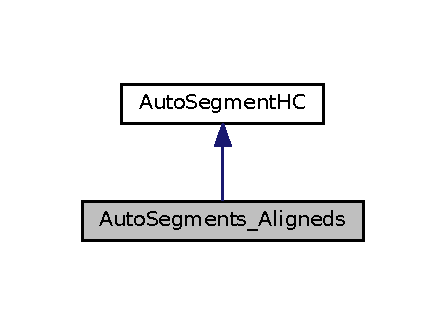
\includegraphics[width=214pt]{classKatabatic_1_1AutoSegments__Aligneds__inherit__graph}
\end{center}
\end{figure}
\subsection*{Public Member Functions}
\begin{DoxyCompactItemize}
\item 
\mbox{\hyperlink{classKatabatic_1_1AutoSegments__Aligneds_a97d48d49a2372cf289d321e6abf81c2d}{Auto\+Segments\+\_\+\+Aligneds}} (\mbox{\hyperlink{classKatabatic_1_1AutoSegment}{Auto\+Segment}} $\ast$, unsigned int flags=Kb\+No\+Flags)
\item 
\mbox{\hyperlink{classKatabatic_1_1AutoSegments__Aligneds_aade683d2c99dc069e2cd5c8b942f8912}{Auto\+Segments\+\_\+\+Aligneds}} (const \mbox{\hyperlink{classKatabatic_1_1AutoSegments__Aligneds}{Auto\+Segments\+\_\+\+Aligneds}} \&)
\item 
virtual \mbox{\hyperlink{namespaceKatabatic_acb3628dc7705fefe38a665cfe43efa6e}{Auto\+Segment\+HC}} $\ast$ \mbox{\hyperlink{classKatabatic_1_1AutoSegments__Aligneds_a5b26b0698bdcb40cbf51b250dfb21858}{get\+Clone}} () const
\item 
virtual \mbox{\hyperlink{namespaceKatabatic_a40ef13471fd0e797b75d3c436813fe65}{Auto\+Segment\+HL}} $\ast$ \mbox{\hyperlink{classKatabatic_1_1AutoSegments__Aligneds_a07665c070fcc269aec02ce842f384483}{get\+Locator}} () const
\end{DoxyCompactItemize}


\subsection{Detailed Description}
All aligned \mbox{\hyperlink{classKatabatic_1_1AutoSegment}{Auto\+Segment}} of a set. 

A Collection to iterate over all the \mbox{\hyperlink{classKatabatic_1_1AutoSegment}{Auto\+Segment}} aligned with {\ttfamily master}. The {\ttfamily master} itself will not be included in the walkthrough. If the \mbox{\hyperlink{namespaceKatabatic_a2af2ad6b6441614038caf59d04b3b217ae2d033c8f78b61468c827de8db5fe839}{Katabatic\+::\+Kb\+With\+Perpands}} flag is passed as argument, the collection will also includes the Auto\+Segments directly perpandicular to the aligned set.

\begin{DoxyParagraph}{Remark\+: Auto\+Segments are forced to be aligneds only when connected through}
\mbox{\hyperlink{classKatabatic_1_1AutoContactHTee}{Auto\+Contact\+H\+Tee}} or \mbox{\hyperlink{classKatabatic_1_1AutoContactVTee}{Auto\+Contact\+V\+Tee}}. 
\end{DoxyParagraph}


\subsection{Constructor \& Destructor Documentation}
\mbox{\Hypertarget{classKatabatic_1_1AutoSegments__Aligneds_a97d48d49a2372cf289d321e6abf81c2d}\label{classKatabatic_1_1AutoSegments__Aligneds_a97d48d49a2372cf289d321e6abf81c2d}} 
\index{Katabatic\+::\+Auto\+Segments\+\_\+\+Aligneds@{Katabatic\+::\+Auto\+Segments\+\_\+\+Aligneds}!Auto\+Segments\+\_\+\+Aligneds@{Auto\+Segments\+\_\+\+Aligneds}}
\index{Auto\+Segments\+\_\+\+Aligneds@{Auto\+Segments\+\_\+\+Aligneds}!Katabatic\+::\+Auto\+Segments\+\_\+\+Aligneds@{Katabatic\+::\+Auto\+Segments\+\_\+\+Aligneds}}
\subsubsection{\texorpdfstring{Auto\+Segments\+\_\+\+Aligneds()}{AutoSegments\_Aligneds()}\hspace{0.1cm}{\footnotesize\ttfamily [1/2]}}
{\footnotesize\ttfamily \mbox{\hyperlink{classKatabatic_1_1AutoSegments__Aligneds}{Auto\+Segments\+\_\+\+Aligneds}} (\begin{DoxyParamCaption}\item[{\mbox{\hyperlink{classKatabatic_1_1AutoSegment}{Auto\+Segment}} $\ast$}]{master,  }\item[{unsigned int}]{flags = {\ttfamily KbNoFlags} }\end{DoxyParamCaption})\hspace{0.3cm}{\ttfamily [inline]}}

Create a collection of all the \mbox{\hyperlink{classKatabatic_1_1AutoSegment}{Auto\+Segment}} aligned on {\ttfamily master} (master itself is excluded from the Collection). If the flag \mbox{\hyperlink{namespaceKatabatic_a2af2ad6b6441614038caf59d04b3b217ae2d033c8f78b61468c827de8db5fe839}{Katabatic\+::\+Kb\+With\+Perpands}} is given the directly perpandicular \mbox{\hyperlink{classKatabatic_1_1AutoSegment}{Auto\+Segment}} will also be includeds. \mbox{\Hypertarget{classKatabatic_1_1AutoSegments__Aligneds_aade683d2c99dc069e2cd5c8b942f8912}\label{classKatabatic_1_1AutoSegments__Aligneds_aade683d2c99dc069e2cd5c8b942f8912}} 
\index{Katabatic\+::\+Auto\+Segments\+\_\+\+Aligneds@{Katabatic\+::\+Auto\+Segments\+\_\+\+Aligneds}!Auto\+Segments\+\_\+\+Aligneds@{Auto\+Segments\+\_\+\+Aligneds}}
\index{Auto\+Segments\+\_\+\+Aligneds@{Auto\+Segments\+\_\+\+Aligneds}!Katabatic\+::\+Auto\+Segments\+\_\+\+Aligneds@{Katabatic\+::\+Auto\+Segments\+\_\+\+Aligneds}}
\subsubsection{\texorpdfstring{Auto\+Segments\+\_\+\+Aligneds()}{AutoSegments\_Aligneds()}\hspace{0.1cm}{\footnotesize\ttfamily [2/2]}}
{\footnotesize\ttfamily \mbox{\hyperlink{classKatabatic_1_1AutoSegments__Aligneds}{Auto\+Segments\+\_\+\+Aligneds}} (\begin{DoxyParamCaption}\item[{const \mbox{\hyperlink{classKatabatic_1_1AutoSegments__Aligneds}{Auto\+Segments\+\_\+\+Aligneds}} \&}]{autosegments }\end{DoxyParamCaption})\hspace{0.3cm}{\ttfamily [inline]}}

Copy constructor. 

\subsection{Member Function Documentation}
\mbox{\Hypertarget{classKatabatic_1_1AutoSegments__Aligneds_a5b26b0698bdcb40cbf51b250dfb21858}\label{classKatabatic_1_1AutoSegments__Aligneds_a5b26b0698bdcb40cbf51b250dfb21858}} 
\index{Katabatic\+::\+Auto\+Segments\+\_\+\+Aligneds@{Katabatic\+::\+Auto\+Segments\+\_\+\+Aligneds}!get\+Clone@{get\+Clone}}
\index{get\+Clone@{get\+Clone}!Katabatic\+::\+Auto\+Segments\+\_\+\+Aligneds@{Katabatic\+::\+Auto\+Segments\+\_\+\+Aligneds}}
\subsubsection{\texorpdfstring{get\+Clone()}{getClone()}}
{\footnotesize\ttfamily \mbox{\hyperlink{namespaceKatabatic_acb3628dc7705fefe38a665cfe43efa6e}{Auto\+Segment\+HC}} $\ast$ get\+Clone (\begin{DoxyParamCaption}{ }\end{DoxyParamCaption}) const\hspace{0.3cm}{\ttfamily [virtual]}}

{\bfseries Returns\+:} A deep copy of the Collection. 

Implements \textbf{ Collection$<$ Type $>$}.

\mbox{\Hypertarget{classKatabatic_1_1AutoSegments__Aligneds_a07665c070fcc269aec02ce842f384483}\label{classKatabatic_1_1AutoSegments__Aligneds_a07665c070fcc269aec02ce842f384483}} 
\index{Katabatic\+::\+Auto\+Segments\+\_\+\+Aligneds@{Katabatic\+::\+Auto\+Segments\+\_\+\+Aligneds}!get\+Locator@{get\+Locator}}
\index{get\+Locator@{get\+Locator}!Katabatic\+::\+Auto\+Segments\+\_\+\+Aligneds@{Katabatic\+::\+Auto\+Segments\+\_\+\+Aligneds}}
\subsubsection{\texorpdfstring{get\+Locator()}{getLocator()}}
{\footnotesize\ttfamily \mbox{\hyperlink{namespaceKatabatic_acb3628dc7705fefe38a665cfe43efa6e}{Auto\+Segment\+HC}} $\ast$ get\+Locator (\begin{DoxyParamCaption}{ }\end{DoxyParamCaption}) const\hspace{0.3cm}{\ttfamily [virtual]}}

{\bfseries Returns\+:} A deep copy of the Collection Locator. 

Implements \textbf{ Collection$<$ Type $>$}.



The documentation for this class was generated from the following files\+:\begin{DoxyCompactItemize}
\item 
Auto\+Segments.\+h\item 
Auto\+Segments.\+dox\end{DoxyCompactItemize}

\hypertarget{classKatabatic_1_1AutoSegments__AnchorOnGCell}{}\section{Auto\+Segments\+\_\+\+Anchor\+On\+G\+Cell Class Reference}
\label{classKatabatic_1_1AutoSegments__AnchorOnGCell}\index{Auto\+Segments\+\_\+\+Anchor\+On\+G\+Cell@{Auto\+Segments\+\_\+\+Anchor\+On\+G\+Cell}}


All \mbox{\hyperlink{classKatabatic_1_1AutoSegment}{Auto\+Segment}} Beginning and/or Stopping in a \mbox{\hyperlink{classKatabatic_1_1GCell}{G\+Cell}}.  




Inheritance diagram for Auto\+Segments\+\_\+\+Anchor\+On\+G\+Cell\+:\nopagebreak
\begin{figure}[H]
\begin{center}
\leavevmode
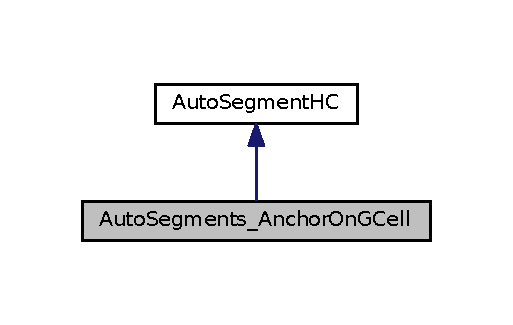
\includegraphics[width=246pt]{classKatabatic_1_1AutoSegments__AnchorOnGCell__inherit__graph}
\end{center}
\end{figure}
\subsection*{Public Member Functions}
\begin{DoxyCompactItemize}
\item 
\mbox{\hyperlink{classKatabatic_1_1AutoSegments__AnchorOnGCell_a41a8dace22db3bdd8ecbf1850344f885}{Auto\+Segments\+\_\+\+Anchor\+On\+G\+Cell}} (\mbox{\hyperlink{classKatabatic_1_1GCell}{G\+Cell}} $\ast$fcell, unsigned int flags)
\item 
\mbox{\hyperlink{classKatabatic_1_1AutoSegments__AnchorOnGCell_a4597cd793ef7f6a5be546b24863f99e8}{Auto\+Segments\+\_\+\+Anchor\+On\+G\+Cell}} (const \mbox{\hyperlink{classKatabatic_1_1AutoSegments__AnchorOnGCell}{Auto\+Segments\+\_\+\+Anchor\+On\+G\+Cell}} \&)
\item 
virtual \mbox{\hyperlink{namespaceKatabatic_acb3628dc7705fefe38a665cfe43efa6e}{Auto\+Segment\+HC}} $\ast$ \mbox{\hyperlink{classKatabatic_1_1AutoSegments__AnchorOnGCell_a5b26b0698bdcb40cbf51b250dfb21858}{get\+Clone}} () const
\item 
virtual \mbox{\hyperlink{namespaceKatabatic_a40ef13471fd0e797b75d3c436813fe65}{Auto\+Segment\+HL}} $\ast$ \mbox{\hyperlink{classKatabatic_1_1AutoSegments__AnchorOnGCell_a07665c070fcc269aec02ce842f384483}{get\+Locator}} () const
\end{DoxyCompactItemize}


\subsection{Detailed Description}
All \mbox{\hyperlink{classKatabatic_1_1AutoSegment}{Auto\+Segment}} Beginning and/or Stopping in a \mbox{\hyperlink{classKatabatic_1_1GCell}{G\+Cell}}. 

A Collection to iterate over all the \mbox{\hyperlink{classKatabatic_1_1AutoSegment}{Auto\+Segment}} that begin from and/or end in a \mbox{\hyperlink{classKatabatic_1_1GCell}{G\+Cell}}. 

\subsection{Constructor \& Destructor Documentation}
\mbox{\Hypertarget{classKatabatic_1_1AutoSegments__AnchorOnGCell_a41a8dace22db3bdd8ecbf1850344f885}\label{classKatabatic_1_1AutoSegments__AnchorOnGCell_a41a8dace22db3bdd8ecbf1850344f885}} 
\index{Katabatic\+::\+Auto\+Segments\+\_\+\+Anchor\+On\+G\+Cell@{Katabatic\+::\+Auto\+Segments\+\_\+\+Anchor\+On\+G\+Cell}!Auto\+Segments\+\_\+\+Anchor\+On\+G\+Cell@{Auto\+Segments\+\_\+\+Anchor\+On\+G\+Cell}}
\index{Auto\+Segments\+\_\+\+Anchor\+On\+G\+Cell@{Auto\+Segments\+\_\+\+Anchor\+On\+G\+Cell}!Katabatic\+::\+Auto\+Segments\+\_\+\+Anchor\+On\+G\+Cell@{Katabatic\+::\+Auto\+Segments\+\_\+\+Anchor\+On\+G\+Cell}}
\subsubsection{\texorpdfstring{Auto\+Segments\+\_\+\+Anchor\+On\+G\+Cell()}{AutoSegments\_AnchorOnGCell()}\hspace{0.1cm}{\footnotesize\ttfamily [1/2]}}
{\footnotesize\ttfamily \mbox{\hyperlink{classKatabatic_1_1AutoSegments__AnchorOnGCell}{Auto\+Segments\+\_\+\+Anchor\+On\+G\+Cell}} (\begin{DoxyParamCaption}\item[{\mbox{\hyperlink{classKatabatic_1_1GCell}{G\+Cell}} $\ast$}]{fcell,  }\item[{unsigned int}]{flags }\end{DoxyParamCaption})\hspace{0.3cm}{\ttfamily [inline]}}

Create a collection of all the \mbox{\hyperlink{classKatabatic_1_1AutoSegment}{Auto\+Segment}} beginning from and/or ending in {\ttfamily fcell}. The set returned by the Collection is selected through {\ttfamily flags} \+:
\begin{DoxyItemize}
\item Katabatic\+::\+Kb\+By\+Source \+: include \mbox{\hyperlink{classKatabatic_1_1AutoSegment}{Auto\+Segment}} starting from {\ttfamily fcell}.
\item Katabatic\+::\+Kb\+By\+Target \+: include \mbox{\hyperlink{classKatabatic_1_1AutoSegment}{Auto\+Segment}} ending in {\ttfamily fcell}.
\item \mbox{\hyperlink{namespaceKatabatic_a2af2ad6b6441614038caf59d04b3b217a1a9045673c5d3c30b067100f1440ae1b}{Katabatic\+::\+Kb\+Horizontal}} \+: include horizontal \mbox{\hyperlink{classKatabatic_1_1AutoSegment}{Auto\+Segment}}.
\item \mbox{\hyperlink{namespaceKatabatic_a2af2ad6b6441614038caf59d04b3b217a284cad95203a27172838b09e396e3590}{Katabatic\+::\+Kb\+Vertical}} \+: include vertical \mbox{\hyperlink{classKatabatic_1_1AutoSegment}{Auto\+Segment}}. 
\end{DoxyItemize}\mbox{\Hypertarget{classKatabatic_1_1AutoSegments__AnchorOnGCell_a4597cd793ef7f6a5be546b24863f99e8}\label{classKatabatic_1_1AutoSegments__AnchorOnGCell_a4597cd793ef7f6a5be546b24863f99e8}} 
\index{Katabatic\+::\+Auto\+Segments\+\_\+\+Anchor\+On\+G\+Cell@{Katabatic\+::\+Auto\+Segments\+\_\+\+Anchor\+On\+G\+Cell}!Auto\+Segments\+\_\+\+Anchor\+On\+G\+Cell@{Auto\+Segments\+\_\+\+Anchor\+On\+G\+Cell}}
\index{Auto\+Segments\+\_\+\+Anchor\+On\+G\+Cell@{Auto\+Segments\+\_\+\+Anchor\+On\+G\+Cell}!Katabatic\+::\+Auto\+Segments\+\_\+\+Anchor\+On\+G\+Cell@{Katabatic\+::\+Auto\+Segments\+\_\+\+Anchor\+On\+G\+Cell}}
\subsubsection{\texorpdfstring{Auto\+Segments\+\_\+\+Anchor\+On\+G\+Cell()}{AutoSegments\_AnchorOnGCell()}\hspace{0.1cm}{\footnotesize\ttfamily [2/2]}}
{\footnotesize\ttfamily \mbox{\hyperlink{classKatabatic_1_1AutoSegments__AnchorOnGCell}{Auto\+Segments\+\_\+\+Anchor\+On\+G\+Cell}} (\begin{DoxyParamCaption}\item[{const \mbox{\hyperlink{classKatabatic_1_1AutoSegments__AnchorOnGCell}{Auto\+Segments\+\_\+\+Anchor\+On\+G\+Cell}} \&}]{autosegments }\end{DoxyParamCaption})\hspace{0.3cm}{\ttfamily [inline]}}

Copy constructor. 

\subsection{Member Function Documentation}
\mbox{\Hypertarget{classKatabatic_1_1AutoSegments__AnchorOnGCell_a5b26b0698bdcb40cbf51b250dfb21858}\label{classKatabatic_1_1AutoSegments__AnchorOnGCell_a5b26b0698bdcb40cbf51b250dfb21858}} 
\index{Katabatic\+::\+Auto\+Segments\+\_\+\+Anchor\+On\+G\+Cell@{Katabatic\+::\+Auto\+Segments\+\_\+\+Anchor\+On\+G\+Cell}!get\+Clone@{get\+Clone}}
\index{get\+Clone@{get\+Clone}!Katabatic\+::\+Auto\+Segments\+\_\+\+Anchor\+On\+G\+Cell@{Katabatic\+::\+Auto\+Segments\+\_\+\+Anchor\+On\+G\+Cell}}
\subsubsection{\texorpdfstring{get\+Clone()}{getClone()}}
{\footnotesize\ttfamily \mbox{\hyperlink{namespaceKatabatic_acb3628dc7705fefe38a665cfe43efa6e}{Auto\+Segment\+HC}} $\ast$ get\+Clone (\begin{DoxyParamCaption}{ }\end{DoxyParamCaption}) const\hspace{0.3cm}{\ttfamily [virtual]}}

{\bfseries Returns\+:} A deep copy of the Collection. 

Implements \textbf{ Collection$<$ Type $>$}.

\mbox{\Hypertarget{classKatabatic_1_1AutoSegments__AnchorOnGCell_a07665c070fcc269aec02ce842f384483}\label{classKatabatic_1_1AutoSegments__AnchorOnGCell_a07665c070fcc269aec02ce842f384483}} 
\index{Katabatic\+::\+Auto\+Segments\+\_\+\+Anchor\+On\+G\+Cell@{Katabatic\+::\+Auto\+Segments\+\_\+\+Anchor\+On\+G\+Cell}!get\+Locator@{get\+Locator}}
\index{get\+Locator@{get\+Locator}!Katabatic\+::\+Auto\+Segments\+\_\+\+Anchor\+On\+G\+Cell@{Katabatic\+::\+Auto\+Segments\+\_\+\+Anchor\+On\+G\+Cell}}
\subsubsection{\texorpdfstring{get\+Locator()}{getLocator()}}
{\footnotesize\ttfamily \mbox{\hyperlink{namespaceKatabatic_acb3628dc7705fefe38a665cfe43efa6e}{Auto\+Segment\+HC}} $\ast$ get\+Locator (\begin{DoxyParamCaption}{ }\end{DoxyParamCaption}) const\hspace{0.3cm}{\ttfamily [virtual]}}

{\bfseries Returns\+:} A deep copy of the Collection Locator. 

Implements \textbf{ Collection$<$ Type $>$}.



The documentation for this class was generated from the following files\+:\begin{DoxyCompactItemize}
\item 
Auto\+Segments.\+h\item 
Auto\+Segments.\+dox\end{DoxyCompactItemize}

\hypertarget{classKatabatic_1_1AutoSegments__InDirection}{}\section{Auto\+Segments\+\_\+\+In\+Direction Class Reference}
\label{classKatabatic_1_1AutoSegments__InDirection}\index{Auto\+Segments\+\_\+\+In\+Direction@{Auto\+Segments\+\_\+\+In\+Direction}}


Filter to select \mbox{\hyperlink{classKatabatic_1_1AutoSegment}{Auto\+Segment}} in a given direction.  




Inheritance diagram for Auto\+Segments\+\_\+\+In\+Direction\+:\nopagebreak
\begin{figure}[H]
\begin{center}
\leavevmode
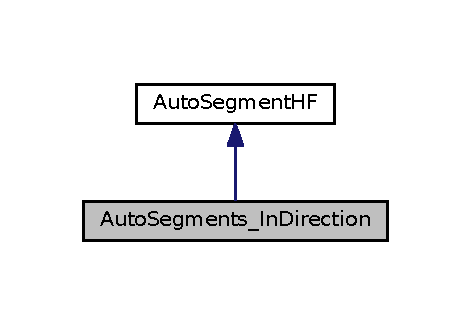
\includegraphics[width=226pt]{classKatabatic_1_1AutoSegments__InDirection__inherit__graph}
\end{center}
\end{figure}
\subsection*{Public Member Functions}
\begin{DoxyCompactItemize}
\item 
\mbox{\hyperlink{classKatabatic_1_1AutoSegments__InDirection_ad51ecb756fa52e994c47dffcdb21c136}{Auto\+Segments\+\_\+\+In\+Direction}} (unsigned int direction)
\item 
virtual \mbox{\hyperlink{namespaceKatabatic_a790418bb65a9a13859868df3e8f53598}{Auto\+Segment\+HF}} $\ast$ \mbox{\hyperlink{classKatabatic_1_1AutoSegments__InDirection_a0a6021852a0c5681a7b53dce6b2b87a4}{get\+Clone}} () const
\item 
virtual bool \mbox{\hyperlink{classKatabatic_1_1AutoSegments__InDirection_adfb5e1308226f0b97fb6825e3eab11a9}{accept}} (\mbox{\hyperlink{classKatabatic_1_1AutoSegment}{Auto\+Segment}} $\ast$segment) const
\end{DoxyCompactItemize}


\subsection{Detailed Description}
Filter to select \mbox{\hyperlink{classKatabatic_1_1AutoSegment}{Auto\+Segment}} in a given direction. 

A Filter to select \mbox{\hyperlink{classKatabatic_1_1AutoSegment}{Auto\+Segment}} in a specific direction. 

\subsection{Constructor \& Destructor Documentation}
\mbox{\Hypertarget{classKatabatic_1_1AutoSegments__InDirection_ad51ecb756fa52e994c47dffcdb21c136}\label{classKatabatic_1_1AutoSegments__InDirection_ad51ecb756fa52e994c47dffcdb21c136}} 
\index{Katabatic\+::\+Auto\+Segments\+\_\+\+In\+Direction@{Katabatic\+::\+Auto\+Segments\+\_\+\+In\+Direction}!Auto\+Segments\+\_\+\+In\+Direction@{Auto\+Segments\+\_\+\+In\+Direction}}
\index{Auto\+Segments\+\_\+\+In\+Direction@{Auto\+Segments\+\_\+\+In\+Direction}!Katabatic\+::\+Auto\+Segments\+\_\+\+In\+Direction@{Katabatic\+::\+Auto\+Segments\+\_\+\+In\+Direction}}
\subsubsection{\texorpdfstring{Auto\+Segments\+\_\+\+In\+Direction()}{AutoSegments\_InDirection()}}
{\footnotesize\ttfamily \mbox{\hyperlink{classKatabatic_1_1AutoSegments__InDirection}{Auto\+Segments\+\_\+\+In\+Direction}} (\begin{DoxyParamCaption}\item[{unsigned int}]{direction }\end{DoxyParamCaption})\hspace{0.3cm}{\ttfamily [inline]}}

Create a filter for \mbox{\hyperlink{classKatabatic_1_1AutoSegment}{Auto\+Segment}} in {\ttfamily direction} (\mbox{\hyperlink{namespaceKatabatic_a2af2ad6b6441614038caf59d04b3b217a1a9045673c5d3c30b067100f1440ae1b}{Katabatic\+::\+Kb\+Horizontal}} or \mbox{\hyperlink{namespaceKatabatic_a2af2ad6b6441614038caf59d04b3b217a284cad95203a27172838b09e396e3590}{Katabatic\+::\+Kb\+Vertical}}). 

\subsection{Member Function Documentation}
\mbox{\Hypertarget{classKatabatic_1_1AutoSegments__InDirection_a0a6021852a0c5681a7b53dce6b2b87a4}\label{classKatabatic_1_1AutoSegments__InDirection_a0a6021852a0c5681a7b53dce6b2b87a4}} 
\index{Katabatic\+::\+Auto\+Segments\+\_\+\+In\+Direction@{Katabatic\+::\+Auto\+Segments\+\_\+\+In\+Direction}!get\+Clone@{get\+Clone}}
\index{get\+Clone@{get\+Clone}!Katabatic\+::\+Auto\+Segments\+\_\+\+In\+Direction@{Katabatic\+::\+Auto\+Segments\+\_\+\+In\+Direction}}
\subsubsection{\texorpdfstring{get\+Clone()}{getClone()}}
{\footnotesize\ttfamily \mbox{\hyperlink{namespaceKatabatic_a790418bb65a9a13859868df3e8f53598}{Auto\+Segment\+HF}} $\ast$ get\+Clone (\begin{DoxyParamCaption}{ }\end{DoxyParamCaption}) const\hspace{0.3cm}{\ttfamily [virtual]}}

{\bfseries Returns\+:} A deep copy of the Collection. 

Implements \textbf{ Filter$<$ Type $>$}.

\mbox{\Hypertarget{classKatabatic_1_1AutoSegments__InDirection_adfb5e1308226f0b97fb6825e3eab11a9}\label{classKatabatic_1_1AutoSegments__InDirection_adfb5e1308226f0b97fb6825e3eab11a9}} 
\index{Katabatic\+::\+Auto\+Segments\+\_\+\+In\+Direction@{Katabatic\+::\+Auto\+Segments\+\_\+\+In\+Direction}!accept@{accept}}
\index{accept@{accept}!Katabatic\+::\+Auto\+Segments\+\_\+\+In\+Direction@{Katabatic\+::\+Auto\+Segments\+\_\+\+In\+Direction}}
\subsubsection{\texorpdfstring{accept()}{accept()}}
{\footnotesize\ttfamily bool accept (\begin{DoxyParamCaption}\item[{\mbox{\hyperlink{classKatabatic_1_1AutoSegment}{Auto\+Segment}} $\ast$}]{segment }\end{DoxyParamCaption}) const\hspace{0.3cm}{\ttfamily [virtual]}}

{\bfseries Returns\+:} {\bfseries true} if the {\ttfamily segment} is in the correct direction. 

The documentation for this class was generated from the following files\+:\begin{DoxyCompactItemize}
\item 
Auto\+Segments.\+h\item 
Auto\+Segments.\+dox\end{DoxyCompactItemize}

\hypertarget{classKatabatic_1_1AutoSegments__IsAccountable}{}\section{Auto\+Segments\+\_\+\+Is\+Accountable Class Reference}
\label{classKatabatic_1_1AutoSegments__IsAccountable}\index{Auto\+Segments\+\_\+\+Is\+Accountable@{Auto\+Segments\+\_\+\+Is\+Accountable}}


Filter to select accoutable \mbox{\hyperlink{classKatabatic_1_1AutoSegment}{Auto\+Segment}}.  




Inheritance diagram for Auto\+Segments\+\_\+\+Is\+Accountable\+:\nopagebreak
\begin{figure}[H]
\begin{center}
\leavevmode
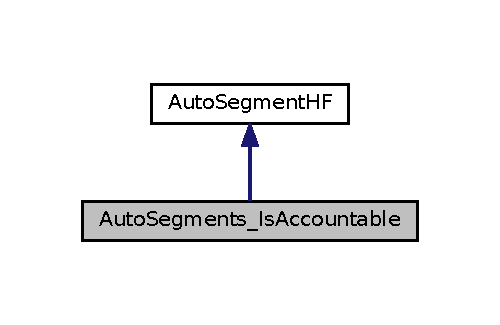
\includegraphics[width=240pt]{classKatabatic_1_1AutoSegments__IsAccountable__inherit__graph}
\end{center}
\end{figure}
\subsection*{Public Member Functions}
\begin{DoxyCompactItemize}
\item 
virtual \mbox{\hyperlink{namespaceKatabatic_a790418bb65a9a13859868df3e8f53598}{Auto\+Segment\+HF}} $\ast$ \mbox{\hyperlink{classKatabatic_1_1AutoSegments__IsAccountable_a0a6021852a0c5681a7b53dce6b2b87a4}{get\+Clone}} () const
\item 
virtual bool \mbox{\hyperlink{classKatabatic_1_1AutoSegments__IsAccountable_a360f3816925114260aeb7ccdab0ea69e}{accept}} (\mbox{\hyperlink{classKatabatic_1_1AutoSegment}{Auto\+Segment}} $\ast$) const
\end{DoxyCompactItemize}


\subsection{Detailed Description}
Filter to select accoutable \mbox{\hyperlink{classKatabatic_1_1AutoSegment}{Auto\+Segment}}. 

A Filter to select accoutable \mbox{\hyperlink{classKatabatic_1_1AutoSegment}{Auto\+Segment}}. An \mbox{\hyperlink{classKatabatic_1_1AutoSegment}{Auto\+Segment}} is said to be accountable if it is canonical (in the sense of an aligned set). 

\subsection{Member Function Documentation}
\mbox{\Hypertarget{classKatabatic_1_1AutoSegments__IsAccountable_a0a6021852a0c5681a7b53dce6b2b87a4}\label{classKatabatic_1_1AutoSegments__IsAccountable_a0a6021852a0c5681a7b53dce6b2b87a4}} 
\index{Katabatic\+::\+Auto\+Segments\+\_\+\+Is\+Accountable@{Katabatic\+::\+Auto\+Segments\+\_\+\+Is\+Accountable}!get\+Clone@{get\+Clone}}
\index{get\+Clone@{get\+Clone}!Katabatic\+::\+Auto\+Segments\+\_\+\+Is\+Accountable@{Katabatic\+::\+Auto\+Segments\+\_\+\+Is\+Accountable}}
\subsubsection{\texorpdfstring{get\+Clone()}{getClone()}}
{\footnotesize\ttfamily \mbox{\hyperlink{namespaceKatabatic_a790418bb65a9a13859868df3e8f53598}{Auto\+Segment\+HF}} $\ast$ get\+Clone (\begin{DoxyParamCaption}{ }\end{DoxyParamCaption}) const\hspace{0.3cm}{\ttfamily [virtual]}}

{\bfseries Returns\+:} A deep copy of the Collection. 

Implements \textbf{ Filter$<$ Type $>$}.

\mbox{\Hypertarget{classKatabatic_1_1AutoSegments__IsAccountable_a360f3816925114260aeb7ccdab0ea69e}\label{classKatabatic_1_1AutoSegments__IsAccountable_a360f3816925114260aeb7ccdab0ea69e}} 
\index{Katabatic\+::\+Auto\+Segments\+\_\+\+Is\+Accountable@{Katabatic\+::\+Auto\+Segments\+\_\+\+Is\+Accountable}!accept@{accept}}
\index{accept@{accept}!Katabatic\+::\+Auto\+Segments\+\_\+\+Is\+Accountable@{Katabatic\+::\+Auto\+Segments\+\_\+\+Is\+Accountable}}
\subsubsection{\texorpdfstring{accept()}{accept()}}
{\footnotesize\ttfamily bool accept (\begin{DoxyParamCaption}\item[{\mbox{\hyperlink{classKatabatic_1_1AutoSegment}{Auto\+Segment}} $\ast$}]{segment }\end{DoxyParamCaption}) const\hspace{0.3cm}{\ttfamily [virtual]}}

{\bfseries Returns\+:} {\bfseries true} if the {\ttfamily segment} is accountable (i.\+e. canonical). 

The documentation for this class was generated from the following files\+:\begin{DoxyCompactItemize}
\item 
Auto\+Segments.\+h\item 
Auto\+Segments.\+dox\end{DoxyCompactItemize}

\hypertarget{classKatabatic_1_1AutoSegments__OnContact}{}\section{Auto\+Segments\+\_\+\+On\+Contact Class Reference}
\label{classKatabatic_1_1AutoSegments__OnContact}\index{Auto\+Segments\+\_\+\+On\+Contact@{Auto\+Segments\+\_\+\+On\+Contact}}


All \mbox{\hyperlink{classKatabatic_1_1AutoSegment}{Auto\+Segment}} anchored on a Contact.  




Inheritance diagram for Auto\+Segments\+\_\+\+On\+Contact\+:\nopagebreak
\begin{figure}[H]
\begin{center}
\leavevmode
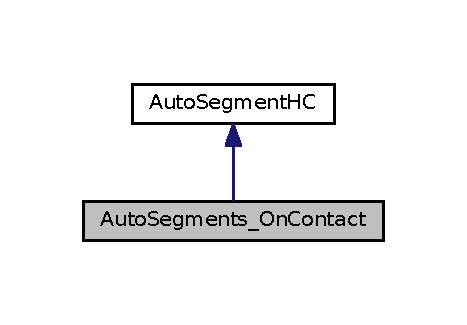
\includegraphics[width=224pt]{classKatabatic_1_1AutoSegments__OnContact__inherit__graph}
\end{center}
\end{figure}
\subsection*{Public Member Functions}
\begin{DoxyCompactItemize}
\item 
\mbox{\hyperlink{classKatabatic_1_1AutoSegments__OnContact_af3f727d0c0fe394da508f52a6c9e4b90}{Auto\+Segments\+\_\+\+On\+Contact}} (\mbox{\hyperlink{classKatabatic_1_1AutoSegment}{Auto\+Segment}} $\ast$master, \textbf{ Contact} $\ast$contact)
\item 
\mbox{\hyperlink{classKatabatic_1_1AutoSegments__OnContact_ab6ff1773c5335fe496f61f2703a5ac99}{Auto\+Segments\+\_\+\+On\+Contact}} (const \mbox{\hyperlink{classKatabatic_1_1AutoSegments__OnContact}{Auto\+Segments\+\_\+\+On\+Contact}} \&)
\item 
virtual \mbox{\hyperlink{namespaceKatabatic_acb3628dc7705fefe38a665cfe43efa6e}{Auto\+Segment\+HC}} $\ast$ \mbox{\hyperlink{classKatabatic_1_1AutoSegments__OnContact_a5b26b0698bdcb40cbf51b250dfb21858}{get\+Clone}} () const
\item 
virtual \mbox{\hyperlink{namespaceKatabatic_a40ef13471fd0e797b75d3c436813fe65}{Auto\+Segment\+HL}} $\ast$ \mbox{\hyperlink{classKatabatic_1_1AutoSegments__OnContact_a07665c070fcc269aec02ce842f384483}{get\+Locator}} () const
\end{DoxyCompactItemize}


\subsection{Detailed Description}
All \mbox{\hyperlink{classKatabatic_1_1AutoSegment}{Auto\+Segment}} anchored on a Contact. 

All \mbox{\hyperlink{classKatabatic_1_1AutoSegment}{Auto\+Segment}} Beginning from an \mbox{\hyperlink{classKatabatic_1_1AutoContact}{Auto\+Contact}}.

A Collection to iterate over all the \mbox{\hyperlink{classKatabatic_1_1AutoSegment}{Auto\+Segment}} anchored on {\ttfamily contact}. If supplied, the \mbox{\hyperlink{classKatabatic_1_1AutoSegment}{Auto\+Segment}} {\ttfamily master} will be excluded from the list.

\begin{DoxyParagraph}{Remark\+: If a Hurricane\+:\+:Segment is anchored on the {\ttfamily contact}, but is not}
associated to an \mbox{\hyperlink{classKatabatic_1_1AutoSegment}{Auto\+Segment}}, it will be silently skipped.
\end{DoxyParagraph}
A Collection to iterate over all the \mbox{\hyperlink{classKatabatic_1_1AutoSegment}{Auto\+Segment}} that begin from \mbox{\hyperlink{classKatabatic_1_1AutoContact}{Auto\+Contact}}. As Auto\+Segments are kept orienteds (source anchor must be lower than target), selecting source anchored Auto\+Segments implies that they are starting from this \mbox{\hyperlink{classKatabatic_1_1AutoContact}{Auto\+Contact}}. 

\subsection{Constructor \& Destructor Documentation}
\mbox{\Hypertarget{classKatabatic_1_1AutoSegments__OnContact_af3f727d0c0fe394da508f52a6c9e4b90}\label{classKatabatic_1_1AutoSegments__OnContact_af3f727d0c0fe394da508f52a6c9e4b90}} 
\index{Katabatic\+::\+Auto\+Segments\+\_\+\+On\+Contact@{Katabatic\+::\+Auto\+Segments\+\_\+\+On\+Contact}!Auto\+Segments\+\_\+\+On\+Contact@{Auto\+Segments\+\_\+\+On\+Contact}}
\index{Auto\+Segments\+\_\+\+On\+Contact@{Auto\+Segments\+\_\+\+On\+Contact}!Katabatic\+::\+Auto\+Segments\+\_\+\+On\+Contact@{Katabatic\+::\+Auto\+Segments\+\_\+\+On\+Contact}}
\subsubsection{\texorpdfstring{Auto\+Segments\+\_\+\+On\+Contact()}{AutoSegments\_OnContact()}\hspace{0.1cm}{\footnotesize\ttfamily [1/2]}}
{\footnotesize\ttfamily \mbox{\hyperlink{classKatabatic_1_1AutoSegments__OnContact}{Auto\+Segments\+\_\+\+On\+Contact}} (\begin{DoxyParamCaption}\item[{\mbox{\hyperlink{classKatabatic_1_1AutoSegment}{Auto\+Segment}} $\ast$}]{master,  }\item[{\textbf{ Contact} $\ast$}]{contact }\end{DoxyParamCaption})\hspace{0.3cm}{\ttfamily [inline]}}


\begin{DoxyParams}{Parameters}
{\em master} & Exclude this \mbox{\hyperlink{classKatabatic_1_1AutoSegment}{Auto\+Segment}} from the Collection. \\
\hline
{\em contact} & The Hurricane Contact over which to iterate.\\
\hline
\end{DoxyParams}
Construct a Collection of all the \mbox{\hyperlink{classKatabatic_1_1AutoSegment}{Auto\+Segment}} anchored on {\ttfamily contact}.

Create the collection of all Auto\+Segments direcly anchored on {\ttfamily contact}, with exclusion of {\ttfamily master}. \mbox{\Hypertarget{classKatabatic_1_1AutoSegments__OnContact_ab6ff1773c5335fe496f61f2703a5ac99}\label{classKatabatic_1_1AutoSegments__OnContact_ab6ff1773c5335fe496f61f2703a5ac99}} 
\index{Katabatic\+::\+Auto\+Segments\+\_\+\+On\+Contact@{Katabatic\+::\+Auto\+Segments\+\_\+\+On\+Contact}!Auto\+Segments\+\_\+\+On\+Contact@{Auto\+Segments\+\_\+\+On\+Contact}}
\index{Auto\+Segments\+\_\+\+On\+Contact@{Auto\+Segments\+\_\+\+On\+Contact}!Katabatic\+::\+Auto\+Segments\+\_\+\+On\+Contact@{Katabatic\+::\+Auto\+Segments\+\_\+\+On\+Contact}}
\subsubsection{\texorpdfstring{Auto\+Segments\+\_\+\+On\+Contact()}{AutoSegments\_OnContact()}\hspace{0.1cm}{\footnotesize\ttfamily [2/2]}}
{\footnotesize\ttfamily \mbox{\hyperlink{classKatabatic_1_1AutoSegments__OnContact}{Auto\+Segments\+\_\+\+On\+Contact}} (\begin{DoxyParamCaption}\item[{const \mbox{\hyperlink{classKatabatic_1_1AutoSegments__OnContact}{Auto\+Segments\+\_\+\+On\+Contact}} \&}]{segments }\end{DoxyParamCaption})\hspace{0.3cm}{\ttfamily [inline]}}

Copy constructor. 

\subsection{Member Function Documentation}
\mbox{\Hypertarget{classKatabatic_1_1AutoSegments__OnContact_a5b26b0698bdcb40cbf51b250dfb21858}\label{classKatabatic_1_1AutoSegments__OnContact_a5b26b0698bdcb40cbf51b250dfb21858}} 
\index{Katabatic\+::\+Auto\+Segments\+\_\+\+On\+Contact@{Katabatic\+::\+Auto\+Segments\+\_\+\+On\+Contact}!get\+Clone@{get\+Clone}}
\index{get\+Clone@{get\+Clone}!Katabatic\+::\+Auto\+Segments\+\_\+\+On\+Contact@{Katabatic\+::\+Auto\+Segments\+\_\+\+On\+Contact}}
\subsubsection{\texorpdfstring{get\+Clone()}{getClone()}}
{\footnotesize\ttfamily \mbox{\hyperlink{namespaceKatabatic_acb3628dc7705fefe38a665cfe43efa6e}{Auto\+Segment\+HC}} $\ast$ get\+Clone (\begin{DoxyParamCaption}{ }\end{DoxyParamCaption}) const\hspace{0.3cm}{\ttfamily [virtual]}}

{\bfseries Returns\+:} A deep copy of the Collection. 

Implements \textbf{ Collection$<$ Type $>$}.

\mbox{\Hypertarget{classKatabatic_1_1AutoSegments__OnContact_a07665c070fcc269aec02ce842f384483}\label{classKatabatic_1_1AutoSegments__OnContact_a07665c070fcc269aec02ce842f384483}} 
\index{Katabatic\+::\+Auto\+Segments\+\_\+\+On\+Contact@{Katabatic\+::\+Auto\+Segments\+\_\+\+On\+Contact}!get\+Locator@{get\+Locator}}
\index{get\+Locator@{get\+Locator}!Katabatic\+::\+Auto\+Segments\+\_\+\+On\+Contact@{Katabatic\+::\+Auto\+Segments\+\_\+\+On\+Contact}}
\subsubsection{\texorpdfstring{get\+Locator()}{getLocator()}}
{\footnotesize\ttfamily \mbox{\hyperlink{namespaceKatabatic_acb3628dc7705fefe38a665cfe43efa6e}{Auto\+Segment\+HC}} $\ast$ get\+Locator (\begin{DoxyParamCaption}{ }\end{DoxyParamCaption}) const\hspace{0.3cm}{\ttfamily [virtual]}}

{\bfseries Returns\+:} A deep copy of the Collection Locator. 

Implements \textbf{ Collection$<$ Type $>$}.



The documentation for this class was generated from the following files\+:\begin{DoxyCompactItemize}
\item 
Auto\+Segments.\+h\item 
Auto\+Segments.\+dox\end{DoxyCompactItemize}

\hypertarget{classKatabatic_1_1AutoSegments__Perpandiculars}{}\section{Auto\+Segments\+\_\+\+Perpandiculars Class Reference}
\label{classKatabatic_1_1AutoSegments__Perpandiculars}\index{Auto\+Segments\+\_\+\+Perpandiculars@{Auto\+Segments\+\_\+\+Perpandiculars}}


All perpandicular \mbox{\hyperlink{classKatabatic_1_1AutoSegment}{Auto\+Segment}} to a set of aligneds.  




Inheritance diagram for Auto\+Segments\+\_\+\+Perpandiculars\+:\nopagebreak
\begin{figure}[H]
\begin{center}
\leavevmode
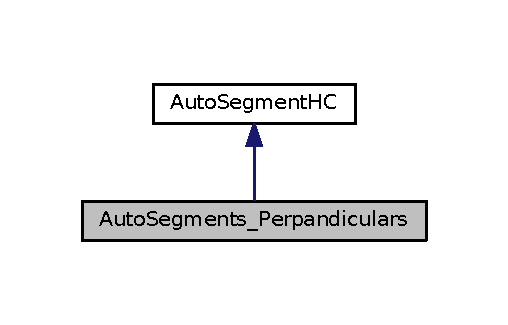
\includegraphics[width=244pt]{classKatabatic_1_1AutoSegments__Perpandiculars__inherit__graph}
\end{center}
\end{figure}
\subsection*{Public Member Functions}
\begin{DoxyCompactItemize}
\item 
\mbox{\hyperlink{classKatabatic_1_1AutoSegments__Perpandiculars_ab5cb1a0042b95cb6bd56997cdfbf0e6f}{Auto\+Segments\+\_\+\+Perpandiculars}} (\mbox{\hyperlink{classKatabatic_1_1AutoSegment}{Auto\+Segment}} $\ast$master)
\item 
\mbox{\hyperlink{classKatabatic_1_1AutoSegments__Perpandiculars_ac2d21dfaa510352fb5c1bd9aa9bd6f94}{Auto\+Segments\+\_\+\+Perpandiculars}} (const \mbox{\hyperlink{classKatabatic_1_1AutoSegments__Perpandiculars}{Auto\+Segments\+\_\+\+Perpandiculars}} \&)
\item 
virtual \mbox{\hyperlink{namespaceKatabatic_acb3628dc7705fefe38a665cfe43efa6e}{Auto\+Segment\+HC}} $\ast$ \mbox{\hyperlink{classKatabatic_1_1AutoSegments__Perpandiculars_a5b26b0698bdcb40cbf51b250dfb21858}{get\+Clone}} () const
\item 
virtual \mbox{\hyperlink{namespaceKatabatic_a40ef13471fd0e797b75d3c436813fe65}{Auto\+Segment\+HL}} $\ast$ \mbox{\hyperlink{classKatabatic_1_1AutoSegments__Perpandiculars_a07665c070fcc269aec02ce842f384483}{get\+Locator}} () const
\end{DoxyCompactItemize}


\subsection{Detailed Description}
All perpandicular \mbox{\hyperlink{classKatabatic_1_1AutoSegment}{Auto\+Segment}} to a set of aligneds. 

A Collection to iterate over all the \mbox{\hyperlink{classKatabatic_1_1AutoSegment}{Auto\+Segment}} perpandicular to the set of aligned \mbox{\hyperlink{classKatabatic_1_1AutoSegment}{Auto\+Segment}} of {\ttfamily master}.

\begin{DoxyParagraph}{Remark\+: This Collection is canonical aware (work on the aligned set).}

\end{DoxyParagraph}


\subsection{Constructor \& Destructor Documentation}
\mbox{\Hypertarget{classKatabatic_1_1AutoSegments__Perpandiculars_ab5cb1a0042b95cb6bd56997cdfbf0e6f}\label{classKatabatic_1_1AutoSegments__Perpandiculars_ab5cb1a0042b95cb6bd56997cdfbf0e6f}} 
\index{Katabatic\+::\+Auto\+Segments\+\_\+\+Perpandiculars@{Katabatic\+::\+Auto\+Segments\+\_\+\+Perpandiculars}!Auto\+Segments\+\_\+\+Perpandiculars@{Auto\+Segments\+\_\+\+Perpandiculars}}
\index{Auto\+Segments\+\_\+\+Perpandiculars@{Auto\+Segments\+\_\+\+Perpandiculars}!Katabatic\+::\+Auto\+Segments\+\_\+\+Perpandiculars@{Katabatic\+::\+Auto\+Segments\+\_\+\+Perpandiculars}}
\subsubsection{\texorpdfstring{Auto\+Segments\+\_\+\+Perpandiculars()}{AutoSegments\_Perpandiculars()}\hspace{0.1cm}{\footnotesize\ttfamily [1/2]}}
{\footnotesize\ttfamily \mbox{\hyperlink{classKatabatic_1_1AutoSegments__Perpandiculars}{Auto\+Segments\+\_\+\+Perpandiculars}} (\begin{DoxyParamCaption}\item[{\mbox{\hyperlink{classKatabatic_1_1AutoSegment}{Auto\+Segment}} $\ast$}]{master }\end{DoxyParamCaption})\hspace{0.3cm}{\ttfamily [inline]}}

Create a collection of all the \mbox{\hyperlink{classKatabatic_1_1AutoSegment}{Auto\+Segment}} perpandicular to the aligned set of {\ttfamily master}. \mbox{\Hypertarget{classKatabatic_1_1AutoSegments__Perpandiculars_ac2d21dfaa510352fb5c1bd9aa9bd6f94}\label{classKatabatic_1_1AutoSegments__Perpandiculars_ac2d21dfaa510352fb5c1bd9aa9bd6f94}} 
\index{Katabatic\+::\+Auto\+Segments\+\_\+\+Perpandiculars@{Katabatic\+::\+Auto\+Segments\+\_\+\+Perpandiculars}!Auto\+Segments\+\_\+\+Perpandiculars@{Auto\+Segments\+\_\+\+Perpandiculars}}
\index{Auto\+Segments\+\_\+\+Perpandiculars@{Auto\+Segments\+\_\+\+Perpandiculars}!Katabatic\+::\+Auto\+Segments\+\_\+\+Perpandiculars@{Katabatic\+::\+Auto\+Segments\+\_\+\+Perpandiculars}}
\subsubsection{\texorpdfstring{Auto\+Segments\+\_\+\+Perpandiculars()}{AutoSegments\_Perpandiculars()}\hspace{0.1cm}{\footnotesize\ttfamily [2/2]}}
{\footnotesize\ttfamily \mbox{\hyperlink{classKatabatic_1_1AutoSegments__Perpandiculars}{Auto\+Segments\+\_\+\+Perpandiculars}} (\begin{DoxyParamCaption}\item[{const \mbox{\hyperlink{classKatabatic_1_1AutoSegments__Perpandiculars}{Auto\+Segments\+\_\+\+Perpandiculars}} \&}]{autosegments }\end{DoxyParamCaption})\hspace{0.3cm}{\ttfamily [inline]}}

Copy constructor. 

\subsection{Member Function Documentation}
\mbox{\Hypertarget{classKatabatic_1_1AutoSegments__Perpandiculars_a5b26b0698bdcb40cbf51b250dfb21858}\label{classKatabatic_1_1AutoSegments__Perpandiculars_a5b26b0698bdcb40cbf51b250dfb21858}} 
\index{Katabatic\+::\+Auto\+Segments\+\_\+\+Perpandiculars@{Katabatic\+::\+Auto\+Segments\+\_\+\+Perpandiculars}!get\+Clone@{get\+Clone}}
\index{get\+Clone@{get\+Clone}!Katabatic\+::\+Auto\+Segments\+\_\+\+Perpandiculars@{Katabatic\+::\+Auto\+Segments\+\_\+\+Perpandiculars}}
\subsubsection{\texorpdfstring{get\+Clone()}{getClone()}}
{\footnotesize\ttfamily \mbox{\hyperlink{namespaceKatabatic_acb3628dc7705fefe38a665cfe43efa6e}{Auto\+Segment\+HC}} $\ast$ get\+Clone (\begin{DoxyParamCaption}{ }\end{DoxyParamCaption}) const\hspace{0.3cm}{\ttfamily [virtual]}}

{\bfseries Returns\+:} A deep copy of the Collection. 

Implements \textbf{ Collection$<$ Type $>$}.

\mbox{\Hypertarget{classKatabatic_1_1AutoSegments__Perpandiculars_a07665c070fcc269aec02ce842f384483}\label{classKatabatic_1_1AutoSegments__Perpandiculars_a07665c070fcc269aec02ce842f384483}} 
\index{Katabatic\+::\+Auto\+Segments\+\_\+\+Perpandiculars@{Katabatic\+::\+Auto\+Segments\+\_\+\+Perpandiculars}!get\+Locator@{get\+Locator}}
\index{get\+Locator@{get\+Locator}!Katabatic\+::\+Auto\+Segments\+\_\+\+Perpandiculars@{Katabatic\+::\+Auto\+Segments\+\_\+\+Perpandiculars}}
\subsubsection{\texorpdfstring{get\+Locator()}{getLocator()}}
{\footnotesize\ttfamily \mbox{\hyperlink{namespaceKatabatic_acb3628dc7705fefe38a665cfe43efa6e}{Auto\+Segment\+HC}} $\ast$ get\+Locator (\begin{DoxyParamCaption}{ }\end{DoxyParamCaption}) const\hspace{0.3cm}{\ttfamily [virtual]}}

{\bfseries Returns\+:} A deep copy of the Collection Locator. 

Implements \textbf{ Collection$<$ Type $>$}.



The documentation for this class was generated from the following files\+:\begin{DoxyCompactItemize}
\item 
Auto\+Segments.\+h\item 
Auto\+Segments.\+dox\end{DoxyCompactItemize}

\hypertarget{classKatabatic_1_1AutoVertical}{}\section{Auto\+Vertical Class Reference}
\label{classKatabatic_1_1AutoVertical}\index{Auto\+Vertical@{Auto\+Vertical}}


Concrete Vertical \mbox{\hyperlink{classKatabatic_1_1AutoSegment}{Auto\+Segment}}.  




Inheritance diagram for Auto\+Vertical\+:\nopagebreak
\begin{figure}[H]
\begin{center}
\leavevmode
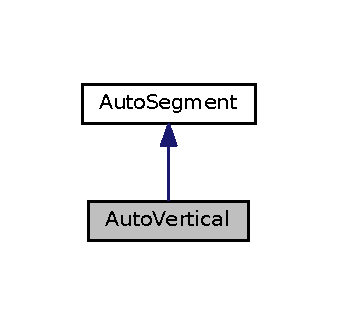
\includegraphics[width=162pt]{classKatabatic_1_1AutoVertical__inherit__graph}
\end{center}
\end{figure}
\subsection*{Public Member Functions}
\begin{DoxyCompactItemize}
\item 
virtual bool \mbox{\hyperlink{classKatabatic_1_1AutoVertical_a2ced98fb06f208aa88c0962a706e64db}{\+\_\+can\+Slacken}} () const
\item 
virtual bool \mbox{\hyperlink{classKatabatic_1_1AutoVertical_a9b0c21eeb26c256876592ba63438da74}{can\+Move\+U\+Left}} (float reserve=0.\+0) const
\item 
virtual bool \mbox{\hyperlink{classKatabatic_1_1AutoVertical_ad0c972e34d6bac47bd9276a7d6e053d8}{can\+Move\+U\+Right}} (float reserve=0.\+0) const
\item 
virtual \textbf{ Segment} $\ast$ \mbox{\hyperlink{classKatabatic_1_1AutoVertical_a9e651c17b47f82166a02865c9296a2df}{base}} ()
\item 
virtual \textbf{ Segment} $\ast$ \mbox{\hyperlink{classKatabatic_1_1AutoVertical_a6f14a3faa93f2c610ea0d2cc7d903706}{base}} () const
\item 
virtual \textbf{ Vertical} $\ast$ \mbox{\hyperlink{classKatabatic_1_1AutoVertical_ab6a809b6f3ef3cf5385fa35580e31e7a}{get\+Vertical}} ()
\item 
virtual \textbf{ Db\+U\+::\+Unit} \mbox{\hyperlink{classKatabatic_1_1AutoVertical_ad521ffba761b0e81b7b81b99d62f76f9}{get\+SourceU}} () const
\item 
virtual \textbf{ Db\+U\+::\+Unit} \mbox{\hyperlink{classKatabatic_1_1AutoVertical_a4d52a506cd19dfa8e22e1dc0695bd960}{get\+TargetU}} () const
\item 
virtual \textbf{ Db\+U\+::\+Unit} \mbox{\hyperlink{classKatabatic_1_1AutoVertical_a760500b1fd027c71f5362dd8c0b01ea7}{get\+Du\+Source}} () const
\item 
virtual \textbf{ Db\+U\+::\+Unit} \mbox{\hyperlink{classKatabatic_1_1AutoVertical_a76e349c14c904b3300a15caa1ee8b680}{get\+Du\+Target}} () const
\item 
virtual \textbf{ Interval} \mbox{\hyperlink{classKatabatic_1_1AutoVertical_a0b5ac47ab175815e1a9bc07f2517614a}{get\+SpanU}} () const
\item 
virtual bool \mbox{\hyperlink{classKatabatic_1_1AutoVertical_a16737e7f2b77f8595fd2b607fac0f2f5}{get\+Constraints}} (\textbf{ Db\+U\+::\+Unit} \&min, \textbf{ Db\+U\+::\+Unit} \&max) const
\item 
virtual \textbf{ Interval} \mbox{\hyperlink{classKatabatic_1_1AutoVertical_a3239751f475bc65adb9d56f6c771ebb0}{get\+Source\+Constraints}} (unsigned int flags=0) const
\item 
virtual \textbf{ Interval} \mbox{\hyperlink{classKatabatic_1_1AutoVertical_ad2b5aeb2604548378c8d78c60862091f}{get\+Target\+Constraints}} (unsigned int flags=0) const
\item 
virtual unsigned int \mbox{\hyperlink{classKatabatic_1_1AutoVertical_a0dd7cf705ace42c662c289955313b2e9}{get\+Direction}} () const
\item 
virtual size\+\_\+t \mbox{\hyperlink{classKatabatic_1_1AutoVertical_accdaef4410043f64da247a94a309733e}{get\+G\+Cells}} (vector$<$ \mbox{\hyperlink{classKatabatic_1_1GCell}{G\+Cell}} $\ast$$>$ \&) const
\item 
virtual void \mbox{\hyperlink{classKatabatic_1_1AutoVertical_a756616a1967c5ad8efd08be96d18f25d}{set\+Du\+Source}} (\textbf{ Db\+U\+::\+Unit})
\item 
virtual void \mbox{\hyperlink{classKatabatic_1_1AutoVertical_a9df2ef68c1fbf4159cc837be5c699b53}{set\+Du\+Target}} (\textbf{ Db\+U\+::\+Unit})
\item 
virtual void \mbox{\hyperlink{classKatabatic_1_1AutoVertical_a59058f4593049c583c5b3698ff81b299}{update\+Orient}} ()
\item 
virtual void \mbox{\hyperlink{classKatabatic_1_1AutoVertical_a9662a77c2ed8553d6a0312c5292060ad}{update\+Positions}} ()
\item 
virtual bool \mbox{\hyperlink{classKatabatic_1_1AutoVertical_a6575c17bfa589c087215c87678e5719c}{check\+Positions}} () const
\item 
virtual bool \mbox{\hyperlink{classKatabatic_1_1AutoVertical_a8aef8f4bbafe3426840f9ebf31bb3b81}{check\+Constraints}} () const
\item 
virtual unsigned int \mbox{\hyperlink{classKatabatic_1_1AutoVertical_a36c0eecad40d3559b5378caefec6a7e0}{\+\_\+make\+Dogleg}} (\mbox{\hyperlink{classKatabatic_1_1GCell}{G\+Cell}} $\ast$, unsigned int flags)
\item 
virtual bool \mbox{\hyperlink{classKatabatic_1_1AutoVertical_a1fa2421b74bf0eb934b7002fd3da2321}{move\+U\+Left}} ()
\item 
virtual bool \mbox{\hyperlink{classKatabatic_1_1AutoVertical_aa469e37853e31f8b1bc817518c896d62}{move\+U\+Right}} ()
\end{DoxyCompactItemize}
\subsection*{Protected Member Functions}
\begin{DoxyCompactItemize}
\item 
virtual void \mbox{\hyperlink{classKatabatic_1_1AutoVertical_a3715b38135ca24745f610bebd3407c10}{\+\_\+post\+Create}} ()
\item 
virtual void \mbox{\hyperlink{classKatabatic_1_1AutoVertical_a7c13d9795eafd477994961f8a0d962d0}{\+\_\+pre\+Destroy}} ()
\end{DoxyCompactItemize}
\subsection*{Additional Inherited Members}


\subsection{Detailed Description}
Concrete Vertical \mbox{\hyperlink{classKatabatic_1_1AutoSegment}{Auto\+Segment}}. 

\subsection{Member Function Documentation}
\mbox{\Hypertarget{classKatabatic_1_1AutoVertical_a2ced98fb06f208aa88c0962a706e64db}\label{classKatabatic_1_1AutoVertical_a2ced98fb06f208aa88c0962a706e64db}} 
\index{Katabatic\+::\+Auto\+Vertical@{Katabatic\+::\+Auto\+Vertical}!\+\_\+can\+Slacken@{\+\_\+can\+Slacken}}
\index{\+\_\+can\+Slacken@{\+\_\+can\+Slacken}!Katabatic\+::\+Auto\+Vertical@{Katabatic\+::\+Auto\+Vertical}}
\subsubsection{\texorpdfstring{\+\_\+can\+Slacken()}{\_canSlacken()}}
{\footnotesize\ttfamily bool \+\_\+can\+Slacken (\begin{DoxyParamCaption}{ }\end{DoxyParamCaption}) const\hspace{0.3cm}{\ttfamily [virtual]}}

{\bfseries Returns\+:} {\bfseries true} if the segment can be slackened. That is, source or target constraints are less than three pitches. 

Implements \mbox{\hyperlink{classKatabatic_1_1AutoSegment_a676fcb7ece71d129b7a4d87a3f2e07aa}{Auto\+Segment}}.



References Interval\+::contains(), Auto\+Segment\+::get\+Auto\+Source(), Auto\+Segment\+::get\+Auto\+Target(), Auto\+Contact\+::get\+G\+Cell(), G\+Cell\+::get\+Side(), Interval\+::inflate(), and Katabatic\+::\+Kb\+Horizontal.

\mbox{\Hypertarget{classKatabatic_1_1AutoVertical_a9b0c21eeb26c256876592ba63438da74}\label{classKatabatic_1_1AutoVertical_a9b0c21eeb26c256876592ba63438da74}} 
\index{Katabatic\+::\+Auto\+Vertical@{Katabatic\+::\+Auto\+Vertical}!can\+Move\+U\+Left@{can\+Move\+U\+Left}}
\index{can\+Move\+U\+Left@{can\+Move\+U\+Left}!Katabatic\+::\+Auto\+Vertical@{Katabatic\+::\+Auto\+Vertical}}
\subsubsection{\texorpdfstring{can\+Move\+U\+Left()}{canMoveULeft()}}
{\footnotesize\ttfamily bool can\+Move\+U\+Left (\begin{DoxyParamCaption}\item[{float}]{reserve = {\ttfamily 0.0} }\end{DoxyParamCaption}) const\hspace{0.3cm}{\ttfamily [virtual]}}

\begin{DoxyReturn}{Returns}
{\bfseries true} if the {\itshape global} segment can be moved on the left \mbox{\hyperlink{classKatabatic_1_1GCell}{G\+Cell}} (for a vertical) or down (for an horizontal). The move is accepted only if it do not change the amount of global wiring. Thus the following conditions\+:
\begin{DoxyItemize}
\item The segment mustn\textquotesingle{}t be on the leftmost \mbox{\hyperlink{classKatabatic_1_1GCell}{G\+Cell}} (obvious...).
\item The segment must be global.
\item The source and target contacts must be Auto\+Contact\+Turn(s).
\item At least one of the perpandicular must be global {\bfseries and} connected through the {\itshape target}. That is, it\textquotesingle{}s a global which extends toward left.
\item The \mbox{\hyperlink{classKatabatic_1_1GCell}{G\+Cell}} of maximum density on the left must remains below the current \mbox{\hyperlink{classKatabatic_1_1GCell}{G\+Cell}} of maximum density, with a margin of {\ttfamily reserve} (expressed in total saturation percentage). 
\end{DoxyItemize}
\end{DoxyReturn}


Implements \mbox{\hyperlink{classKatabatic_1_1AutoSegment_aad55626c9d793a0b08bcff5be2a5ad0c}{Auto\+Segment}}.



References Auto\+Segment\+::get\+Auto\+Source(), Auto\+Segment\+::get\+Auto\+Target(), Auto\+Contact\+::get\+G\+Cell(), Auto\+Segment\+::get\+G\+Cell(), Auto\+Segment\+::get\+Layer(), Routing\+Gauge\+::get\+Layer\+Depth(), G\+Cell\+::get\+Left(), Session\+::get\+Routing\+Gauge(), Auto\+Contact\+::get\+Segment(), G\+Cell\+::get\+Up(), G\+Cell\+::get\+W\+Density(), and Auto\+Segment\+::is\+Global().

\mbox{\Hypertarget{classKatabatic_1_1AutoVertical_ad0c972e34d6bac47bd9276a7d6e053d8}\label{classKatabatic_1_1AutoVertical_ad0c972e34d6bac47bd9276a7d6e053d8}} 
\index{Katabatic\+::\+Auto\+Vertical@{Katabatic\+::\+Auto\+Vertical}!can\+Move\+U\+Right@{can\+Move\+U\+Right}}
\index{can\+Move\+U\+Right@{can\+Move\+U\+Right}!Katabatic\+::\+Auto\+Vertical@{Katabatic\+::\+Auto\+Vertical}}
\subsubsection{\texorpdfstring{can\+Move\+U\+Right()}{canMoveURight()}}
{\footnotesize\ttfamily bool can\+Move\+U\+Right (\begin{DoxyParamCaption}\item[{float}]{reserve = {\ttfamily 0.0} }\end{DoxyParamCaption}) const\hspace{0.3cm}{\ttfamily [virtual]}}

\begin{DoxyReturn}{Returns}
{\bfseries true} if the {\itshape global} segment can be moved on the right \mbox{\hyperlink{classKatabatic_1_1GCell}{G\+Cell}} (for a vertical) or up (for an horizontal). The move is accepted only if it do not change the amount of global wiring. Thus the following conditions\+:
\begin{DoxyItemize}
\item The segment mustn\textquotesingle{}t be on the leftmost \mbox{\hyperlink{classKatabatic_1_1GCell}{G\+Cell}} (obvious...).
\item The segment must be global.
\item The source and target contacts must be Auto\+Contact\+Turn(s).
\item At least one of the perpandicular must be global {\bfseries and} connected through the {\itshape source}. That is, it\textquotesingle{}s a global which extends toward right.
\item The \mbox{\hyperlink{classKatabatic_1_1GCell}{G\+Cell}} of maximum density on the left must remains below the current \mbox{\hyperlink{classKatabatic_1_1GCell}{G\+Cell}} of maximum density, with a margin of {\ttfamily reserve} (expressed in total saturation percentage). 
\end{DoxyItemize}
\end{DoxyReturn}


Implements \mbox{\hyperlink{classKatabatic_1_1AutoSegment_a096deb8a143f098eac2bff9ab9c52243}{Auto\+Segment}}.



References Auto\+Segment\+::get\+Auto\+Source(), Auto\+Segment\+::get\+Auto\+Target(), Auto\+Contact\+::get\+G\+Cell(), Auto\+Segment\+::get\+G\+Cell(), Auto\+Segment\+::get\+Layer(), Routing\+Gauge\+::get\+Layer\+Depth(), G\+Cell\+::get\+Right(), Session\+::get\+Routing\+Gauge(), Auto\+Contact\+::get\+Segment(), G\+Cell\+::get\+Up(), G\+Cell\+::get\+W\+Density(), and Auto\+Segment\+::is\+Global().

\mbox{\Hypertarget{classKatabatic_1_1AutoVertical_a9e651c17b47f82166a02865c9296a2df}\label{classKatabatic_1_1AutoVertical_a9e651c17b47f82166a02865c9296a2df}} 
\index{Katabatic\+::\+Auto\+Vertical@{Katabatic\+::\+Auto\+Vertical}!base@{base}}
\index{base@{base}!Katabatic\+::\+Auto\+Vertical@{Katabatic\+::\+Auto\+Vertical}}
\subsubsection{\texorpdfstring{base()}{base()}\hspace{0.1cm}{\footnotesize\ttfamily [1/2]}}
{\footnotesize\ttfamily \textbf{ Segment} $\ast$ base (\begin{DoxyParamCaption}{ }\end{DoxyParamCaption})\hspace{0.3cm}{\ttfamily [virtual]}}

{\bfseries Returns\+:} the decorated \textbf{ Hurricane\+::\+Segment}. 

Implements \mbox{\hyperlink{classKatabatic_1_1AutoSegment_ade416d0483aefe986988fa89a7cf6fcf}{Auto\+Segment}}.

\mbox{\Hypertarget{classKatabatic_1_1AutoVertical_a6f14a3faa93f2c610ea0d2cc7d903706}\label{classKatabatic_1_1AutoVertical_a6f14a3faa93f2c610ea0d2cc7d903706}} 
\index{Katabatic\+::\+Auto\+Vertical@{Katabatic\+::\+Auto\+Vertical}!base@{base}}
\index{base@{base}!Katabatic\+::\+Auto\+Vertical@{Katabatic\+::\+Auto\+Vertical}}
\subsubsection{\texorpdfstring{base()}{base()}\hspace{0.1cm}{\footnotesize\ttfamily [2/2]}}
{\footnotesize\ttfamily \textbf{ Segment} $\ast$ base (\begin{DoxyParamCaption}{ }\end{DoxyParamCaption}) const\hspace{0.3cm}{\ttfamily [virtual]}}

{\bfseries Returns\+:} the decorated \textbf{ Hurricane\+::\+Segment} (const flavor). 

Implements \mbox{\hyperlink{classKatabatic_1_1AutoSegment_a53877ff5ef48eb0030c2581a6eeb3c09}{Auto\+Segment}}.

\mbox{\Hypertarget{classKatabatic_1_1AutoVertical_ab6a809b6f3ef3cf5385fa35580e31e7a}\label{classKatabatic_1_1AutoVertical_ab6a809b6f3ef3cf5385fa35580e31e7a}} 
\index{Katabatic\+::\+Auto\+Vertical@{Katabatic\+::\+Auto\+Vertical}!get\+Vertical@{get\+Vertical}}
\index{get\+Vertical@{get\+Vertical}!Katabatic\+::\+Auto\+Vertical@{Katabatic\+::\+Auto\+Vertical}}
\subsubsection{\texorpdfstring{get\+Vertical()}{getVertical()}}
{\footnotesize\ttfamily \textbf{ Vertical} $\ast$ get\+Vertical (\begin{DoxyParamCaption}{ }\end{DoxyParamCaption})\hspace{0.3cm}{\ttfamily [virtual]}}

{\bfseries Returns\+:} If the decorated segment is a \textbf{ Hurricane\+::\+Vertical}, return it. {\ttfamily N\+U\+LL} otherwise. 

Reimplemented from \mbox{\hyperlink{classKatabatic_1_1AutoSegment_ab6a809b6f3ef3cf5385fa35580e31e7a}{Auto\+Segment}}.

\mbox{\Hypertarget{classKatabatic_1_1AutoVertical_ad521ffba761b0e81b7b81b99d62f76f9}\label{classKatabatic_1_1AutoVertical_ad521ffba761b0e81b7b81b99d62f76f9}} 
\index{Katabatic\+::\+Auto\+Vertical@{Katabatic\+::\+Auto\+Vertical}!get\+SourceU@{get\+SourceU}}
\index{get\+SourceU@{get\+SourceU}!Katabatic\+::\+Auto\+Vertical@{Katabatic\+::\+Auto\+Vertical}}
\subsubsection{\texorpdfstring{get\+Source\+U()}{getSourceU()}}
{\footnotesize\ttfamily \textbf{ Db\+U\+::\+Unit} get\+SourceU (\begin{DoxyParamCaption}{ }\end{DoxyParamCaption}) const\hspace{0.3cm}{\ttfamily [virtual]}}

{\bfseries Returns\+:} The \mbox{\hyperlink{classKatabatic_1_1AutoSegment}{Auto\+Segment}} {\itshape uniform} source position. (X for an horizontal and Y for a Vertical). 

Implements \mbox{\hyperlink{classKatabatic_1_1AutoSegment_aeaa1543880686755e389c4807128428f}{Auto\+Segment}}.



References Segment\+::get\+Source\+Y().

\mbox{\Hypertarget{classKatabatic_1_1AutoVertical_a4d52a506cd19dfa8e22e1dc0695bd960}\label{classKatabatic_1_1AutoVertical_a4d52a506cd19dfa8e22e1dc0695bd960}} 
\index{Katabatic\+::\+Auto\+Vertical@{Katabatic\+::\+Auto\+Vertical}!get\+TargetU@{get\+TargetU}}
\index{get\+TargetU@{get\+TargetU}!Katabatic\+::\+Auto\+Vertical@{Katabatic\+::\+Auto\+Vertical}}
\subsubsection{\texorpdfstring{get\+Target\+U()}{getTargetU()}}
{\footnotesize\ttfamily \textbf{ Db\+U\+::\+Unit} get\+TargetU (\begin{DoxyParamCaption}{ }\end{DoxyParamCaption}) const\hspace{0.3cm}{\ttfamily [virtual]}}

{\bfseries Returns\+:} The \mbox{\hyperlink{classKatabatic_1_1AutoSegment}{Auto\+Segment}} {\itshape uniform} target position. (X for an horizontal and Y for a Vertical). 

Implements \mbox{\hyperlink{classKatabatic_1_1AutoSegment_a828fef2716cc9c370d6d170bb96556ec}{Auto\+Segment}}.



References Segment\+::get\+Target\+Y().

\mbox{\Hypertarget{classKatabatic_1_1AutoVertical_a760500b1fd027c71f5362dd8c0b01ea7}\label{classKatabatic_1_1AutoVertical_a760500b1fd027c71f5362dd8c0b01ea7}} 
\index{Katabatic\+::\+Auto\+Vertical@{Katabatic\+::\+Auto\+Vertical}!get\+Du\+Source@{get\+Du\+Source}}
\index{get\+Du\+Source@{get\+Du\+Source}!Katabatic\+::\+Auto\+Vertical@{Katabatic\+::\+Auto\+Vertical}}
\subsubsection{\texorpdfstring{get\+Du\+Source()}{getDuSource()}}
{\footnotesize\ttfamily \textbf{ Db\+U\+::\+Unit} get\+Du\+Source (\begin{DoxyParamCaption}{ }\end{DoxyParamCaption}) const\hspace{0.3cm}{\ttfamily [virtual]}}

{\bfseries Returns\+:} The \mbox{\hyperlink{classKatabatic_1_1AutoSegment}{Auto\+Segment}} {\itshape uniform} delta from source. (dX for an horizontal and dY for a Vertical). 

Implements \mbox{\hyperlink{classKatabatic_1_1AutoSegment_ab4881df67bd8f036d0199ed6540fe774}{Auto\+Segment}}.



References Vertical\+::get\+Dy\+Source().

\mbox{\Hypertarget{classKatabatic_1_1AutoVertical_a76e349c14c904b3300a15caa1ee8b680}\label{classKatabatic_1_1AutoVertical_a76e349c14c904b3300a15caa1ee8b680}} 
\index{Katabatic\+::\+Auto\+Vertical@{Katabatic\+::\+Auto\+Vertical}!get\+Du\+Target@{get\+Du\+Target}}
\index{get\+Du\+Target@{get\+Du\+Target}!Katabatic\+::\+Auto\+Vertical@{Katabatic\+::\+Auto\+Vertical}}
\subsubsection{\texorpdfstring{get\+Du\+Target()}{getDuTarget()}}
{\footnotesize\ttfamily \textbf{ Db\+U\+::\+Unit} get\+Du\+Target (\begin{DoxyParamCaption}{ }\end{DoxyParamCaption}) const\hspace{0.3cm}{\ttfamily [virtual]}}

{\bfseries Returns\+:} The \mbox{\hyperlink{classKatabatic_1_1AutoSegment}{Auto\+Segment}} {\itshape uniform} delta from source. (dX for an horizontal and dY for a Vertical). 

Implements \mbox{\hyperlink{classKatabatic_1_1AutoSegment_a0644d656eedc71dba2fb3c6c0d83ed3f}{Auto\+Segment}}.



References Vertical\+::get\+Dy\+Target().

\mbox{\Hypertarget{classKatabatic_1_1AutoVertical_a0b5ac47ab175815e1a9bc07f2517614a}\label{classKatabatic_1_1AutoVertical_a0b5ac47ab175815e1a9bc07f2517614a}} 
\index{Katabatic\+::\+Auto\+Vertical@{Katabatic\+::\+Auto\+Vertical}!get\+SpanU@{get\+SpanU}}
\index{get\+SpanU@{get\+SpanU}!Katabatic\+::\+Auto\+Vertical@{Katabatic\+::\+Auto\+Vertical}}
\subsubsection{\texorpdfstring{get\+Span\+U()}{getSpanU()}}
{\footnotesize\ttfamily \textbf{ Interval} get\+SpanU (\begin{DoxyParamCaption}{ }\end{DoxyParamCaption}) const\hspace{0.3cm}{\ttfamily [virtual]}}

{\bfseries Returns\+:} The \mbox{\hyperlink{classKatabatic_1_1AutoSegment}{Auto\+Segment}} {\itshape uniform} occupying interval (on X for horizontal and on Y for vertical). 

Implements \mbox{\hyperlink{classKatabatic_1_1AutoSegment_a248eb2fbb06e3286650b28567d495f0b}{Auto\+Segment}}.



References Segment\+::get\+Source\+Y(), and Segment\+::get\+Target\+Y().

\mbox{\Hypertarget{classKatabatic_1_1AutoVertical_a16737e7f2b77f8595fd2b607fac0f2f5}\label{classKatabatic_1_1AutoVertical_a16737e7f2b77f8595fd2b607fac0f2f5}} 
\index{Katabatic\+::\+Auto\+Vertical@{Katabatic\+::\+Auto\+Vertical}!get\+Constraints@{get\+Constraints}}
\index{get\+Constraints@{get\+Constraints}!Katabatic\+::\+Auto\+Vertical@{Katabatic\+::\+Auto\+Vertical}}
\subsubsection{\texorpdfstring{get\+Constraints()}{getConstraints()}}
{\footnotesize\ttfamily bool get\+Constraints (\begin{DoxyParamCaption}\item[{\textbf{ Db\+U\+::\+Unit} \&}]{min,  }\item[{\textbf{ Db\+U\+::\+Unit} \&}]{max }\end{DoxyParamCaption}) const\hspace{0.3cm}{\ttfamily [virtual]}}

{\bfseries Returns\+:} in {\ttfamily min} \& {\ttfamily max} the allowed range for the segment axis. 

Implements \mbox{\hyperlink{classKatabatic_1_1AutoSegment_a7c2fed22b081f8d3b7a69abb457153ea}{Auto\+Segment}}.



References Auto\+Segment\+::get\+Auto\+Source(), Auto\+Segment\+::get\+Auto\+Target(), Auto\+Contact\+::get\+C\+B\+X\+Max(), Auto\+Contact\+::get\+C\+B\+X\+Min(), Auto\+Segment\+::get\+User\+Constraints(), and Db\+U\+::get\+Value\+String().

\mbox{\Hypertarget{classKatabatic_1_1AutoVertical_a3239751f475bc65adb9d56f6c771ebb0}\label{classKatabatic_1_1AutoVertical_a3239751f475bc65adb9d56f6c771ebb0}} 
\index{Katabatic\+::\+Auto\+Vertical@{Katabatic\+::\+Auto\+Vertical}!get\+Source\+Constraints@{get\+Source\+Constraints}}
\index{get\+Source\+Constraints@{get\+Source\+Constraints}!Katabatic\+::\+Auto\+Vertical@{Katabatic\+::\+Auto\+Vertical}}
\subsubsection{\texorpdfstring{get\+Source\+Constraints()}{getSourceConstraints()}}
{\footnotesize\ttfamily \textbf{ Interval} get\+Source\+Constraints (\begin{DoxyParamCaption}\item[{unsigned int}]{flags = {\ttfamily 0} }\end{DoxyParamCaption}) const\hspace{0.3cm}{\ttfamily [virtual]}}

\begin{DoxyReturn}{Returns}
The Interval into witch the source \mbox{\hyperlink{classKatabatic_1_1AutoContact}{Auto\+Contact}} can vary. By default all deduced constraints and user constraints are took into account. If {\ttfamily flags} contains {\ttfamily Kb\+Native\+Constraints} the constraint returned is only the enclosing \mbox{\hyperlink{classKatabatic_1_1GCell}{G\+Cell}}. 
\end{DoxyReturn}


Implements \mbox{\hyperlink{classKatabatic_1_1AutoSegment_ab7685e309e1d910db3e8237f8a898c35}{Auto\+Segment}}.



References Auto\+Segment\+::get\+Auto\+Source(), Box\+::get\+X\+Max(), Box\+::get\+X\+Min(), and Katabatic\+::\+Kb\+Native\+Constraints.

\mbox{\Hypertarget{classKatabatic_1_1AutoVertical_ad2b5aeb2604548378c8d78c60862091f}\label{classKatabatic_1_1AutoVertical_ad2b5aeb2604548378c8d78c60862091f}} 
\index{Katabatic\+::\+Auto\+Vertical@{Katabatic\+::\+Auto\+Vertical}!get\+Target\+Constraints@{get\+Target\+Constraints}}
\index{get\+Target\+Constraints@{get\+Target\+Constraints}!Katabatic\+::\+Auto\+Vertical@{Katabatic\+::\+Auto\+Vertical}}
\subsubsection{\texorpdfstring{get\+Target\+Constraints()}{getTargetConstraints()}}
{\footnotesize\ttfamily \textbf{ Interval} get\+Target\+Constraints (\begin{DoxyParamCaption}\item[{unsigned int}]{flags = {\ttfamily 0} }\end{DoxyParamCaption}) const\hspace{0.3cm}{\ttfamily [virtual]}}

\begin{DoxyReturn}{Returns}
The Interval into witch the target \mbox{\hyperlink{classKatabatic_1_1AutoContact}{Auto\+Contact}} can vary. By default all deduced constraints and user constraints are took into account. If {\ttfamily flags} contains {\ttfamily Kb\+Native\+Constraints} the constraint returned is only the enclosing \mbox{\hyperlink{classKatabatic_1_1GCell}{G\+Cell}}. 
\end{DoxyReturn}


Implements \mbox{\hyperlink{classKatabatic_1_1AutoSegment_a9c1b8b3cd57fb7b0bf60c7a6148237c2}{Auto\+Segment}}.



References Auto\+Segment\+::get\+Auto\+Target(), Box\+::get\+X\+Max(), Box\+::get\+X\+Min(), and Katabatic\+::\+Kb\+Native\+Constraints.

\mbox{\Hypertarget{classKatabatic_1_1AutoVertical_a0dd7cf705ace42c662c289955313b2e9}\label{classKatabatic_1_1AutoVertical_a0dd7cf705ace42c662c289955313b2e9}} 
\index{Katabatic\+::\+Auto\+Vertical@{Katabatic\+::\+Auto\+Vertical}!get\+Direction@{get\+Direction}}
\index{get\+Direction@{get\+Direction}!Katabatic\+::\+Auto\+Vertical@{Katabatic\+::\+Auto\+Vertical}}
\subsubsection{\texorpdfstring{get\+Direction()}{getDirection()}}
{\footnotesize\ttfamily unsigned int get\+Direction (\begin{DoxyParamCaption}{ }\end{DoxyParamCaption}) const\hspace{0.3cm}{\ttfamily [virtual]}}

{\bfseries Returns\+:} \mbox{\hyperlink{namespaceKatabatic_a2af2ad6b6441614038caf59d04b3b217a1a9045673c5d3c30b067100f1440ae1b}{Katabatic\+::\+Kb\+Horizontal}} or \mbox{\hyperlink{namespaceKatabatic_a2af2ad6b6441614038caf59d04b3b217a284cad95203a27172838b09e396e3590}{Katabatic\+::\+Kb\+Vertical}} according to the decorated segment. 

Implements \mbox{\hyperlink{classKatabatic_1_1AutoSegment_ae35b78590ed6aa546b626ef95f28c533}{Auto\+Segment}}.



References Katabatic\+::\+Kb\+Vertical.

\mbox{\Hypertarget{classKatabatic_1_1AutoVertical_accdaef4410043f64da247a94a309733e}\label{classKatabatic_1_1AutoVertical_accdaef4410043f64da247a94a309733e}} 
\index{Katabatic\+::\+Auto\+Vertical@{Katabatic\+::\+Auto\+Vertical}!get\+G\+Cells@{get\+G\+Cells}}
\index{get\+G\+Cells@{get\+G\+Cells}!Katabatic\+::\+Auto\+Vertical@{Katabatic\+::\+Auto\+Vertical}}
\subsubsection{\texorpdfstring{get\+G\+Cells()}{getGCells()}}
{\footnotesize\ttfamily size\+\_\+t get\+G\+Cells (\begin{DoxyParamCaption}\item[{vector$<$ \mbox{\hyperlink{classKatabatic_1_1GCell}{G\+Cell}} $\ast$$>$ \&}]{gcells }\end{DoxyParamCaption}) const\hspace{0.3cm}{\ttfamily [virtual]}}


\begin{DoxyParams}{Parameters}
{\em gcells} & A vector that will be filled by all the G\+Cells that the segment overlap. In increasing order, from source to target. \\
\hline
\end{DoxyParams}
\begin{DoxyReturn}{Returns}
The vector\textquotesingle{}s size. 
\end{DoxyReturn}


Implements \mbox{\hyperlink{classKatabatic_1_1AutoSegment_a8ca0022e253d355817d46a057ae01625}{Auto\+Segment}}.



References Auto\+Segment\+::get\+Auto\+Source(), Auto\+Segment\+::get\+Auto\+Target(), Auto\+Contact\+::get\+G\+Cell(), Auto\+Segment\+::get\+G\+Cell(), and G\+Cell\+::get\+Up().

\mbox{\Hypertarget{classKatabatic_1_1AutoVertical_a756616a1967c5ad8efd08be96d18f25d}\label{classKatabatic_1_1AutoVertical_a756616a1967c5ad8efd08be96d18f25d}} 
\index{Katabatic\+::\+Auto\+Vertical@{Katabatic\+::\+Auto\+Vertical}!set\+Du\+Source@{set\+Du\+Source}}
\index{set\+Du\+Source@{set\+Du\+Source}!Katabatic\+::\+Auto\+Vertical@{Katabatic\+::\+Auto\+Vertical}}
\subsubsection{\texorpdfstring{set\+Du\+Source()}{setDuSource()}}
{\footnotesize\ttfamily void set\+Du\+Source (\begin{DoxyParamCaption}\item[{\textbf{ Db\+U\+::\+Unit}}]{du }\end{DoxyParamCaption})\hspace{0.3cm}{\ttfamily [virtual]}}

Set the {\itshape uniform} {\ttfamily dU} from source anchor (dX for Horizontal, dY for Vertical). 

Implements \mbox{\hyperlink{classKatabatic_1_1AutoSegment_aaf60d18ab6d951a34a3d06959ce2e76f}{Auto\+Segment}}.

\mbox{\Hypertarget{classKatabatic_1_1AutoVertical_a9df2ef68c1fbf4159cc837be5c699b53}\label{classKatabatic_1_1AutoVertical_a9df2ef68c1fbf4159cc837be5c699b53}} 
\index{Katabatic\+::\+Auto\+Vertical@{Katabatic\+::\+Auto\+Vertical}!set\+Du\+Target@{set\+Du\+Target}}
\index{set\+Du\+Target@{set\+Du\+Target}!Katabatic\+::\+Auto\+Vertical@{Katabatic\+::\+Auto\+Vertical}}
\subsubsection{\texorpdfstring{set\+Du\+Target()}{setDuTarget()}}
{\footnotesize\ttfamily void set\+Du\+Target (\begin{DoxyParamCaption}\item[{\textbf{ Db\+U\+::\+Unit}}]{du }\end{DoxyParamCaption})\hspace{0.3cm}{\ttfamily [virtual]}}

Set the {\itshape uniform} {\ttfamily dU} from target anchor (dX for Horizontal, dY for Vertical). 

Implements \mbox{\hyperlink{classKatabatic_1_1AutoSegment_a246756d4c8b3e094a0a9d6de3c2109ff}{Auto\+Segment}}.

\mbox{\Hypertarget{classKatabatic_1_1AutoVertical_a59058f4593049c583c5b3698ff81b299}\label{classKatabatic_1_1AutoVertical_a59058f4593049c583c5b3698ff81b299}} 
\index{Katabatic\+::\+Auto\+Vertical@{Katabatic\+::\+Auto\+Vertical}!update\+Orient@{update\+Orient}}
\index{update\+Orient@{update\+Orient}!Katabatic\+::\+Auto\+Vertical@{Katabatic\+::\+Auto\+Vertical}}
\subsubsection{\texorpdfstring{update\+Orient()}{updateOrient()}}
{\footnotesize\ttfamily void update\+Orient (\begin{DoxyParamCaption}{ }\end{DoxyParamCaption})\hspace{0.3cm}{\ttfamily [virtual]}}

Ensure that source is lower than target. Swap them if needed. Swap never occurs on global segment because their source and target anchors are from different \mbox{\hyperlink{classKatabatic_1_1GCell}{G\+Cell}}, which are already ordered. 

Implements \mbox{\hyperlink{classKatabatic_1_1AutoSegment_a102e0f4bbb0386e41be214d15a9e4549}{Auto\+Segment}}.



References Segment\+::get\+Source\+Y(), Segment\+::get\+Target\+Y(), Segment\+::invert(), Katabatic\+::\+Seg\+Source\+Bottom, Katabatic\+::\+Seg\+Source\+Top, Katabatic\+::\+Seg\+Target\+Bottom, Katabatic\+::\+Seg\+Target\+Top, Auto\+Segment\+::set\+Flags(), and Auto\+Segment\+::unset\+Flags().

\mbox{\Hypertarget{classKatabatic_1_1AutoVertical_a9662a77c2ed8553d6a0312c5292060ad}\label{classKatabatic_1_1AutoVertical_a9662a77c2ed8553d6a0312c5292060ad}} 
\index{Katabatic\+::\+Auto\+Vertical@{Katabatic\+::\+Auto\+Vertical}!update\+Positions@{update\+Positions}}
\index{update\+Positions@{update\+Positions}!Katabatic\+::\+Auto\+Vertical@{Katabatic\+::\+Auto\+Vertical}}
\subsubsection{\texorpdfstring{update\+Positions()}{updatePositions()}}
{\footnotesize\ttfamily void update\+Positions (\begin{DoxyParamCaption}{ }\end{DoxyParamCaption})\hspace{0.3cm}{\ttfamily [virtual]}}

Update the segment begenning and ending positions. The positions takes into account the extension caps and reflect the real space used by the segment under it\textquotesingle{}s long axis. 

Implements \mbox{\hyperlink{classKatabatic_1_1AutoSegment_a6d95f4de39c13611786c95ddc7b8942e}{Auto\+Segment}}.



References Session\+::get\+Extension\+Cap(), Auto\+Segment\+::get\+Layer(), Segment\+::get\+Source\+Y(), and Segment\+::get\+Target\+Y().

\mbox{\Hypertarget{classKatabatic_1_1AutoVertical_a6575c17bfa589c087215c87678e5719c}\label{classKatabatic_1_1AutoVertical_a6575c17bfa589c087215c87678e5719c}} 
\index{Katabatic\+::\+Auto\+Vertical@{Katabatic\+::\+Auto\+Vertical}!check\+Positions@{check\+Positions}}
\index{check\+Positions@{check\+Positions}!Katabatic\+::\+Auto\+Vertical@{Katabatic\+::\+Auto\+Vertical}}
\subsubsection{\texorpdfstring{check\+Positions()}{checkPositions()}}
{\footnotesize\ttfamily bool check\+Positions (\begin{DoxyParamCaption}{ }\end{DoxyParamCaption}) const\hspace{0.3cm}{\ttfamily [virtual]}}

{\bfseries Returns\+:} {\bfseries true} if the relative positions of source \& target are coherent. (source $<$= target). 

Implements \mbox{\hyperlink{classKatabatic_1_1AutoSegment_af026a81002bd907f1ccd4a4784aaa1db}{Auto\+Segment}}.



References Session\+::get\+Extension\+Cap(), Auto\+Segment\+::get\+Layer(), Segment\+::get\+Source\+Y(), Segment\+::get\+Target\+Y(), and Db\+U\+::get\+Value\+String().

\mbox{\Hypertarget{classKatabatic_1_1AutoVertical_a8aef8f4bbafe3426840f9ebf31bb3b81}\label{classKatabatic_1_1AutoVertical_a8aef8f4bbafe3426840f9ebf31bb3b81}} 
\index{Katabatic\+::\+Auto\+Vertical@{Katabatic\+::\+Auto\+Vertical}!check\+Constraints@{check\+Constraints}}
\index{check\+Constraints@{check\+Constraints}!Katabatic\+::\+Auto\+Vertical@{Katabatic\+::\+Auto\+Vertical}}
\subsubsection{\texorpdfstring{check\+Constraints()}{checkConstraints()}}
{\footnotesize\ttfamily bool check\+Constraints (\begin{DoxyParamCaption}{ }\end{DoxyParamCaption}) const\hspace{0.3cm}{\ttfamily [virtual]}}

{\bfseries Returns\+:} {\bfseries true} if the constraint intervel is coherent (non-\/empty or punctual in the worst case). 

Implements \mbox{\hyperlink{classKatabatic_1_1AutoSegment_a3d5732fd10b4a05076981066a4674487}{Auto\+Segment}}.



References Auto\+Segment\+::get\+Auto\+Source(), Auto\+Segment\+::get\+Auto\+Target(), and Interval\+::intersect().

\mbox{\Hypertarget{classKatabatic_1_1AutoVertical_a36c0eecad40d3559b5378caefec6a7e0}\label{classKatabatic_1_1AutoVertical_a36c0eecad40d3559b5378caefec6a7e0}} 
\index{Katabatic\+::\+Auto\+Vertical@{Katabatic\+::\+Auto\+Vertical}!\+\_\+make\+Dogleg@{\+\_\+make\+Dogleg}}
\index{\+\_\+make\+Dogleg@{\+\_\+make\+Dogleg}!Katabatic\+::\+Auto\+Vertical@{Katabatic\+::\+Auto\+Vertical}}
\subsubsection{\texorpdfstring{\+\_\+make\+Dogleg()}{\_makeDogleg()}}
{\footnotesize\ttfamily unsigned int \+\_\+make\+Dogleg (\begin{DoxyParamCaption}\item[{\mbox{\hyperlink{classKatabatic_1_1GCell}{G\+Cell}} $\ast$}]{dogleg\+G\+Cell,  }\item[{unsigned int}]{flags }\end{DoxyParamCaption})\hspace{0.3cm}{\ttfamily [virtual]}}

{\bfseries This method is the workhorse for the various dogleg and topology restauration methods.} It is the atomic method that actually make the dogleg on {\bfseries this} segment.

{\bfseries Returns\+:} \mbox{\hyperlink{namespaceKatabatic_a2af2ad6b6441614038caf59d04b3b217af756099f1bbe259dd1bf22067dc40eac}{Katabatic\+::\+Kb\+Use\+Above\+Layer}} if the dogleg is using the {\itshape above} layer (\mbox{\hyperlink{namespaceKatabatic_a2af2ad6b6441614038caf59d04b3b217a41cbd981337678e042354f340bfae25d}{Katabatic\+::\+Kb\+Use\+Below\+Layer}} for the below layer).

Break the current segment in two (a.\+k.\+a. making a dogleg).
\begin{DoxyItemize}
\item The segment is broken inside {\ttfamily dogleg\+G\+Cell}.
\item Two new segments are createds, one perpandicular and one parallel.
\item The original segment is always kept attached to the {\itshape source}. (the new parallel fragment is attached to the {\itshape target}).
\item The perpandicular segment is in the layer {\itshape above} by default. If we are already on the topmost routing layer, the {\itshape below} layer is used.
\item If the segment pass through the breaking \mbox{\hyperlink{classKatabatic_1_1GCell}{G\+Cell}}, it\textquotesingle{}s axis is set into the center. If the segment is local, the axis is the middle of the segment.
\item The Local/\+Global kind of the original segment is updated. The local/global status is computed by the constructor of the \mbox{\hyperlink{classKatabatic_1_1AutoSegment}{Auto\+Segment}} for the perpandicular and the new parallel.
\item The terminal state is updated. If the segment is a strong terminal the part that is no longer directly connected to the terminal is demoted to \mbox{\hyperlink{namespaceKatabatic_a94585537ee1724ea9315578ec54380f4a7b3e09b8ab4cf676fd308535d7fba892}{Katabatic\+::\+Seg\+Weak\+Terminal1}}.
\item The perpandicular is obviously a canonical. If the broken segment is canonical, the original {\bfseries is} left canonical and only the new parallel is re-\/canonized. Otherwise, we re-\/canonise both sets of aligned segments (the one on the source and the one on the target).
\item The three segments are added to the session dogleg stack.
\end{DoxyItemize}

After this method call the net topology is guarantee to be valid.

  

Implements \mbox{\hyperlink{classKatabatic_1_1AutoSegment_a37a14b40295ccb50cd5001891385807b}{Auto\+Segment}}.



References Auto\+Contact\+::base(), Auto\+Segment\+::canonize(), Auto\+Contact\+Turn\+::create(), Auto\+Segment\+::create(), Session\+::dogleg(), Auto\+Segment\+::get\+Auto\+Source(), Auto\+Segment\+::get\+Auto\+Target(), Session\+::get\+Configuration(), Routing\+Gauge\+::get\+Contact\+Layer(), Auto\+Contact\+::get\+G\+Cell(), Component\+::get\+Layer(), Auto\+Segment\+::get\+Layer(), Routing\+Gauge\+::get\+Layer\+Depth(), Component\+::get\+Net(), Session\+::get\+Routing\+Gauge(), Routing\+Gauge\+::get\+Routing\+Layer(), Auto\+Segment\+::get\+Source\+Y(), Auto\+Segment\+::get\+Target\+Y(), G\+Cell\+::get\+Up(), Auto\+Segment\+::get\+X(), G\+Cell\+::get\+Y(), G\+Cell\+::get\+Y\+Max(), Auto\+Contact\+::invalidate(), Auto\+Segment\+::invalidate(), Auto\+Segment\+::is\+Canonical(), Auto\+Segment\+::is\+Local(), Auto\+Segment\+::is\+Slackened(), Auto\+Segment\+::is\+Weak\+Terminal(), Katabatic\+::\+Kb\+Horizontal, Katabatic\+::\+Kb\+Use\+Above\+Layer, Katabatic\+::\+Kb\+Use\+Below\+Layer, Katabatic\+::\+Kb\+Vertical, Auto\+Contact\+::migrate\+Constraint\+Box(), G\+Cell\+::remove\+V\+Segment(), Katabatic\+::\+Seg\+Canonical, Katabatic\+::\+Seg\+Dogleg, Katabatic\+::\+Seg\+Global, Katabatic\+::\+Seg\+Not\+Aligned, Katabatic\+::\+Seg\+Slackened, Katabatic\+::\+Seg\+Weak\+Terminal1, Auto\+Segment\+::set\+Flags(), Auto\+Segment\+::set\+Layer(), and Auto\+Segment\+::unset\+Flags().

\mbox{\Hypertarget{classKatabatic_1_1AutoVertical_a1fa2421b74bf0eb934b7002fd3da2321}\label{classKatabatic_1_1AutoVertical_a1fa2421b74bf0eb934b7002fd3da2321}} 
\index{Katabatic\+::\+Auto\+Vertical@{Katabatic\+::\+Auto\+Vertical}!move\+U\+Left@{move\+U\+Left}}
\index{move\+U\+Left@{move\+U\+Left}!Katabatic\+::\+Auto\+Vertical@{Katabatic\+::\+Auto\+Vertical}}
\subsubsection{\texorpdfstring{move\+U\+Left()}{moveULeft()}}
{\footnotesize\ttfamily bool move\+U\+Left (\begin{DoxyParamCaption}{ }\end{DoxyParamCaption})\hspace{0.3cm}{\ttfamily [virtual]}}

{\bfseries This function do not manage an aligned set. It applies on {\ttfamily this} segment only.}

Displace an Horizontal or Vertical segment to the \mbox{\hyperlink{classKatabatic_1_1GCell}{G\+Cell}} below (a.\+k.\+a. lower or inferior). Rules for displacement\+:
\begin{DoxyItemize}
\item The segment must be connected at both end to a turn contact (we do not want to manage more complex cases for the time beeing).
\item And, of course, the segment must not already by on the bottomost \mbox{\hyperlink{classKatabatic_1_1GCell}{G\+Cell}}...
\end{DoxyItemize}

The displacement take care of\+:
\begin{DoxyItemize}
\item Managing the status of the various perpandiculars. The stretched one are made global if needed. The shrinked one made local, if needed.
\item The supporting \mbox{\hyperlink{classKatabatic_1_1AutoContact}{Auto\+Contact}} (source \& target) are changed of \mbox{\hyperlink{classKatabatic_1_1GCell}{G\+Cell}}.
\item If the segment is global, the go-\/through G\+Cells are updateds.
\end{DoxyItemize}

{\bfseries Returns\+:} {\bfseries true} if the move has succeeded.

 

Implements \mbox{\hyperlink{classKatabatic_1_1AutoSegment_af8ca7b17e952f4b599aeeb2f4e5be395}{Auto\+Segment}}.



References G\+Cell\+::add\+H\+Segment(), Auto\+Segment\+::get\+Auto\+Source(), Auto\+Segment\+::get\+Auto\+Target(), Auto\+Contact\+::get\+G\+Cell(), Auto\+Segment\+::get\+G\+Cell(), G\+Cell\+::get\+Left(), Auto\+Contact\+::get\+Segment(), G\+Cell\+::get\+Side(), G\+Cell\+::get\+Up(), Interval\+::get\+V\+Max(), Auto\+Segment\+::is\+Local(), Katabatic\+::\+Kb\+Horizontal, G\+Cell\+::remove\+H\+Segment(), Katabatic\+::\+Seg\+Global, Auto\+Segment\+::set\+Axis(), Auto\+Segment\+::set\+Flags(), Auto\+Contact\+::set\+G\+Cell(), and Auto\+Segment\+::unset\+Flags().

\mbox{\Hypertarget{classKatabatic_1_1AutoVertical_aa469e37853e31f8b1bc817518c896d62}\label{classKatabatic_1_1AutoVertical_aa469e37853e31f8b1bc817518c896d62}} 
\index{Katabatic\+::\+Auto\+Vertical@{Katabatic\+::\+Auto\+Vertical}!move\+U\+Right@{move\+U\+Right}}
\index{move\+U\+Right@{move\+U\+Right}!Katabatic\+::\+Auto\+Vertical@{Katabatic\+::\+Auto\+Vertical}}
\subsubsection{\texorpdfstring{move\+U\+Right()}{moveURight()}}
{\footnotesize\ttfamily bool move\+U\+Right (\begin{DoxyParamCaption}{ }\end{DoxyParamCaption})\hspace{0.3cm}{\ttfamily [virtual]}}

{\bfseries This function do not manage an aligned set. It applies on {\ttfamily this} segment only.}

Displace an Horizontal or Vertical segment to the \mbox{\hyperlink{classKatabatic_1_1GCell}{G\+Cell}} above (a.\+k.\+a. upper or superior). Rules for displacement\+:

\begin{DoxySeeAlso}{See also}
\mbox{\hyperlink{classKatabatic_1_1AutoSegment_af8ca7b17e952f4b599aeeb2f4e5be395}{Auto\+Segment\+::move\+U\+Left()}} for a complete description. 
\end{DoxySeeAlso}


Implements \mbox{\hyperlink{classKatabatic_1_1AutoSegment_ad7fd54ca229fcf5ccd99f87b019b9cbc}{Auto\+Segment}}.



References G\+Cell\+::add\+H\+Segment(), Auto\+Segment\+::get\+Auto\+Source(), Auto\+Segment\+::get\+Auto\+Target(), Auto\+Contact\+::get\+G\+Cell(), Auto\+Segment\+::get\+G\+Cell(), G\+Cell\+::get\+Right(), Auto\+Contact\+::get\+Segment(), G\+Cell\+::get\+Side(), G\+Cell\+::get\+Up(), Db\+U\+::get\+Value\+String(), Interval\+::get\+V\+Min(), Auto\+Segment\+::is\+Local(), Katabatic\+::\+Kb\+Horizontal, G\+Cell\+::remove\+H\+Segment(), Katabatic\+::\+Seg\+Global, Auto\+Segment\+::set\+Axis(), Auto\+Segment\+::set\+Flags(), Auto\+Contact\+::set\+G\+Cell(), and Auto\+Segment\+::unset\+Flags().

\mbox{\Hypertarget{classKatabatic_1_1AutoVertical_a3715b38135ca24745f610bebd3407c10}\label{classKatabatic_1_1AutoVertical_a3715b38135ca24745f610bebd3407c10}} 
\index{Katabatic\+::\+Auto\+Vertical@{Katabatic\+::\+Auto\+Vertical}!\+\_\+post\+Create@{\+\_\+post\+Create}}
\index{\+\_\+post\+Create@{\+\_\+post\+Create}!Katabatic\+::\+Auto\+Vertical@{Katabatic\+::\+Auto\+Vertical}}
\subsubsection{\texorpdfstring{\+\_\+post\+Create()}{\_postCreate()}}
{\footnotesize\ttfamily void \+\_\+post\+Create (\begin{DoxyParamCaption}{ }\end{DoxyParamCaption})\hspace{0.3cm}{\ttfamily [protected]}, {\ttfamily [virtual]}}

In addition to \mbox{\hyperlink{classKatabatic_1_1AutoSegment_a3715b38135ca24745f610bebd3407c10}{Auto\+Segment\+::\+\_\+post\+Create()}}, detect whether the segment is global or local and register it in the relevant G\+Cells (if needed).

If the segment is anchored directly on a terminal, adjust the axis so it\textquotesingle{}s connected. 

Reimplemented from \mbox{\hyperlink{classKatabatic_1_1AutoSegment_a3715b38135ca24745f610bebd3407c10}{Auto\+Segment}}.



References Auto\+Segment\+::\+\_\+post\+Create(), G\+Cell\+::add\+V\+Segment(), Auto\+Segment\+::get\+Auto\+Source(), Auto\+Segment\+::get\+Auto\+Target(), Auto\+Contact\+::get\+G\+Cell(), G\+Cell\+::get\+Up(), Component\+::get\+X(), G\+Cell\+::get\+Y(), Katabatic\+::\+Seg\+Global, Auto\+Segment\+::set\+Flags(), and Auto\+Contact\+::set\+X().

\mbox{\Hypertarget{classKatabatic_1_1AutoVertical_a7c13d9795eafd477994961f8a0d962d0}\label{classKatabatic_1_1AutoVertical_a7c13d9795eafd477994961f8a0d962d0}} 
\index{Katabatic\+::\+Auto\+Vertical@{Katabatic\+::\+Auto\+Vertical}!\+\_\+pre\+Destroy@{\+\_\+pre\+Destroy}}
\index{\+\_\+pre\+Destroy@{\+\_\+pre\+Destroy}!Katabatic\+::\+Auto\+Vertical@{Katabatic\+::\+Auto\+Vertical}}
\subsubsection{\texorpdfstring{\+\_\+pre\+Destroy()}{\_preDestroy()}}
{\footnotesize\ttfamily void \+\_\+pre\+Destroy (\begin{DoxyParamCaption}{ }\end{DoxyParamCaption})\hspace{0.3cm}{\ttfamily [protected]}, {\ttfamily [virtual]}}

Perform operations that must be done before the actual destructor is called. Merely whidrawn the \mbox{\hyperlink{classKatabatic_1_1AutoSegment}{Auto\+Segment}} from the lookup/\+Session mechanism. 

Reimplemented from \mbox{\hyperlink{classKatabatic_1_1AutoSegment_a7c13d9795eafd477994961f8a0d962d0}{Auto\+Segment}}.



References Auto\+Segment\+::\+\_\+pre\+Destroy(), Auto\+Segment\+::get\+Auto\+Source(), Auto\+Segment\+::get\+Auto\+Target(), Auto\+Contact\+::get\+G\+Cell(), Auto\+Segment\+::get\+Id(), G\+Cell\+::get\+Up(), G\+Cell\+::get\+Y(), and G\+Cell\+::remove\+V\+Segment().



The documentation for this class was generated from the following files\+:\begin{DoxyCompactItemize}
\item 
Auto\+Vertical.\+h\item 
Auto\+Vertical.\+cpp\item 
Auto\+Vertical.\+dox\end{DoxyCompactItemize}

\hypertarget{classKatabatic_1_1BaseGrid_1_1Axis}{}\section{Base\+Grid\+:\+:Axis Class Reference}
\label{classKatabatic_1_1BaseGrid_1_1Axis}\index{Base\+Grid\+::\+Axis@{Base\+Grid\+::\+Axis}}


Graduations on a \mbox{\hyperlink{classKatabatic_1_1BaseGrid}{Base\+Grid}} \mbox{\hyperlink{classKatabatic_1_1BaseGrid_1_1Axis}{Axis}} (H or V).  


\subsection*{Public Member Functions}
\begin{DoxyCompactItemize}
\item 
void \mbox{\hyperlink{classKatabatic_1_1BaseGrid_1_1Axis_ada526136545060f41e8b9228ce1c5895}{add\+Graduation}} (\textbf{ Db\+U\+::\+Unit})
\item 
void \mbox{\hyperlink{classKatabatic_1_1BaseGrid_1_1Axis_a47fdc9eea42b6975cdc835bb2e08810e}{sort}} ()
\item 
unsigned int \mbox{\hyperlink{classKatabatic_1_1BaseGrid_1_1Axis_a9be1e4285daa77fe397767c097fbdc66}{get\+Size}} () const
\item 
unsigned int \mbox{\hyperlink{classKatabatic_1_1BaseGrid_1_1Axis_a2a6bd524227130d8ccf482aa2c484a42}{get\+Graduation\+Number}} (\textbf{ Db\+U\+::\+Unit} pos, bool \&on\+Graduation) const
\item 
const \textbf{ Db\+U\+::\+Unit} \& \mbox{\hyperlink{classKatabatic_1_1BaseGrid_1_1Axis_a074a4f61306b88baac6bbf54b0b3212c}{operator\mbox{[}$\,$\mbox{]}}} (unsigned int i) const
\end{DoxyCompactItemize}


\subsection{Detailed Description}
Graduations on a \mbox{\hyperlink{classKatabatic_1_1BaseGrid}{Base\+Grid}} \mbox{\hyperlink{classKatabatic_1_1BaseGrid_1_1Axis}{Axis}} (H or V). 

Describe the list of graduations on either X or Y axis of a \mbox{\hyperlink{classKatabatic_1_1BaseGrid}{Base\+Grid}}. Graduations correspond to cut lines and may not be evenly spaced.

Graduations are internally stored into a vector that needs to be sorted whenever new graduations are added (\mbox{\hyperlink{classKatabatic_1_1BaseGrid_1_1Axis_a47fdc9eea42b6975cdc835bb2e08810e}{Base\+Grid\+::\+Axis\+::sort()}}). 

\subsection{Member Function Documentation}
\mbox{\Hypertarget{classKatabatic_1_1BaseGrid_1_1Axis_ada526136545060f41e8b9228ce1c5895}\label{classKatabatic_1_1BaseGrid_1_1Axis_ada526136545060f41e8b9228ce1c5895}} 
\index{Katabatic\+::\+Base\+Grid\+::\+Axis@{Katabatic\+::\+Base\+Grid\+::\+Axis}!add\+Graduation@{add\+Graduation}}
\index{add\+Graduation@{add\+Graduation}!Katabatic\+::\+Base\+Grid\+::\+Axis@{Katabatic\+::\+Base\+Grid\+::\+Axis}}
\subsubsection{\texorpdfstring{add\+Graduation()}{addGraduation()}}
{\footnotesize\ttfamily void add\+Graduation (\begin{DoxyParamCaption}\item[{\textbf{ Db\+U\+::\+Unit}}]{pos }\end{DoxyParamCaption})\hspace{0.3cm}{\ttfamily [inline]}}

Adds a new graduation. After adding new graduations, do not forget to perform a sort. 

Referenced by G\+Cell\+Grid\+::\+\_\+post\+Create().

\mbox{\Hypertarget{classKatabatic_1_1BaseGrid_1_1Axis_a47fdc9eea42b6975cdc835bb2e08810e}\label{classKatabatic_1_1BaseGrid_1_1Axis_a47fdc9eea42b6975cdc835bb2e08810e}} 
\index{Katabatic\+::\+Base\+Grid\+::\+Axis@{Katabatic\+::\+Base\+Grid\+::\+Axis}!sort@{sort}}
\index{sort@{sort}!Katabatic\+::\+Base\+Grid\+::\+Axis@{Katabatic\+::\+Base\+Grid\+::\+Axis}}
\subsubsection{\texorpdfstring{sort()}{sort()}}
{\footnotesize\ttfamily void sort (\begin{DoxyParamCaption}{ }\end{DoxyParamCaption})}

Re-\/order the graduations after an addition. 

Referenced by G\+Cell\+Grid\+::\+\_\+post\+Create().

\mbox{\Hypertarget{classKatabatic_1_1BaseGrid_1_1Axis_a9be1e4285daa77fe397767c097fbdc66}\label{classKatabatic_1_1BaseGrid_1_1Axis_a9be1e4285daa77fe397767c097fbdc66}} 
\index{Katabatic\+::\+Base\+Grid\+::\+Axis@{Katabatic\+::\+Base\+Grid\+::\+Axis}!get\+Size@{get\+Size}}
\index{get\+Size@{get\+Size}!Katabatic\+::\+Base\+Grid\+::\+Axis@{Katabatic\+::\+Base\+Grid\+::\+Axis}}
\subsubsection{\texorpdfstring{get\+Size()}{getSize()}}
{\footnotesize\ttfamily size\+\_\+t get\+Size (\begin{DoxyParamCaption}{ }\end{DoxyParamCaption}) const\hspace{0.3cm}{\ttfamily [inline]}}

{\bfseries Returns\+:} The number of graduations on the axis. 

Referenced by G\+Cell\+Grid\+::\+\_\+post\+Create().

\mbox{\Hypertarget{classKatabatic_1_1BaseGrid_1_1Axis_a2a6bd524227130d8ccf482aa2c484a42}\label{classKatabatic_1_1BaseGrid_1_1Axis_a2a6bd524227130d8ccf482aa2c484a42}} 
\index{Katabatic\+::\+Base\+Grid\+::\+Axis@{Katabatic\+::\+Base\+Grid\+::\+Axis}!get\+Graduation\+Number@{get\+Graduation\+Number}}
\index{get\+Graduation\+Number@{get\+Graduation\+Number}!Katabatic\+::\+Base\+Grid\+::\+Axis@{Katabatic\+::\+Base\+Grid\+::\+Axis}}
\subsubsection{\texorpdfstring{get\+Graduation\+Number()}{getGraduationNumber()}}
{\footnotesize\ttfamily \textbf{ Db\+U\+::\+Unit} get\+Graduation\+Number (\begin{DoxyParamCaption}\item[{\textbf{ Db\+U\+::\+Unit}}]{pos,  }\item[{bool \&}]{on\+Graduation }\end{DoxyParamCaption}) const}

{\bfseries Returns\+:} The index of the graduation which is immediatly inferior or equal to {\ttfamily pos}. In case of strict equality, {\ttfamily on\+Graduation} is set to {\bfseries true}. \mbox{\Hypertarget{classKatabatic_1_1BaseGrid_1_1Axis_a074a4f61306b88baac6bbf54b0b3212c}\label{classKatabatic_1_1BaseGrid_1_1Axis_a074a4f61306b88baac6bbf54b0b3212c}} 
\index{Katabatic\+::\+Base\+Grid\+::\+Axis@{Katabatic\+::\+Base\+Grid\+::\+Axis}!operator\mbox{[}\mbox{]}@{operator[]}}
\index{operator\mbox{[}\mbox{]}@{operator[]}!Katabatic\+::\+Base\+Grid\+::\+Axis@{Katabatic\+::\+Base\+Grid\+::\+Axis}}
\subsubsection{\texorpdfstring{operator[]()}{operator[]()}}
{\footnotesize\ttfamily \textbf{ Db\+U\+::\+Unit} operator\mbox{[}$\,$\mbox{]} (\begin{DoxyParamCaption}\item[{unsigned int}]{index }\end{DoxyParamCaption}) const\hspace{0.3cm}{\ttfamily [inline]}}

{\bfseries Returns\+:} The graduation at {\ttfamily index}. 

The documentation for this class was generated from the following files\+:\begin{DoxyCompactItemize}
\item 
Grid.\+h\item 
Grid.\+cpp\item 
Grid.\+dox\end{DoxyCompactItemize}

\hypertarget{classKatabatic_1_1BaseGrid}{}\section{Base\+Grid Class Reference}
\label{classKatabatic_1_1BaseGrid}\index{Base\+Grid@{Base\+Grid}}


Abstract Base Class for Irregular \mbox{\hyperlink{classKatabatic_1_1Grid}{Grid}}.  




Inheritance diagram for Base\+Grid\+:\nopagebreak
\begin{figure}[H]
\begin{center}
\leavevmode
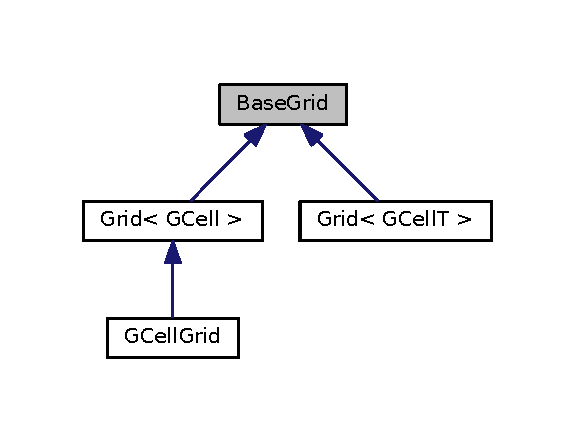
\includegraphics[width=276pt]{classKatabatic_1_1BaseGrid__inherit__graph}
\end{center}
\end{figure}
\subsection*{Classes}
\begin{DoxyCompactItemize}
\item 
class \mbox{\hyperlink{classKatabatic_1_1BaseGrid_1_1Axis}{Axis}}
\begin{DoxyCompactList}\small\item\em Graduations on a \mbox{\hyperlink{classKatabatic_1_1BaseGrid}{Base\+Grid}} \mbox{\hyperlink{classKatabatic_1_1BaseGrid_1_1Axis}{Axis}} (H or V). \end{DoxyCompactList}\end{DoxyCompactItemize}
\subsection*{Public Member Functions}
\begin{DoxyCompactItemize}
\item 
void \mbox{\hyperlink{classKatabatic_1_1BaseGrid_a3a80b6032f86a56bec74609034b3246f}{destroy}} ()
\item 
const \textbf{ Box} \& \mbox{\hyperlink{classKatabatic_1_1BaseGrid_a4b6cf5a28d88d7ad3e6ddeac28a35a0b}{get\+Bounding\+Box}} () const
\item 
unsigned int \mbox{\hyperlink{classKatabatic_1_1BaseGrid_aeaf0dae788f4c997e6172f9c734e3a91}{get\+Columns}} () const
\item 
unsigned int \mbox{\hyperlink{classKatabatic_1_1BaseGrid_a4bad6abc58473d953258a3230506291a}{get\+Rows}} () const
\item 
unsigned int \mbox{\hyperlink{classKatabatic_1_1BaseGrid_a47cf844f090417180d0bae098133565e}{get\+Raw\+Size}} () const
\item 
unsigned int \mbox{\hyperlink{classKatabatic_1_1BaseGrid_aae84726d9984c1df9905fc97d9b34f28}{get\+Index}} (unsigned int c, unsigned int r) const
\item 
unsigned int \mbox{\hyperlink{classKatabatic_1_1BaseGrid_a8108a276ab72226244d302fb1b59f3f1}{get\+Row}} (unsigned int) const
\item 
unsigned int \mbox{\hyperlink{classKatabatic_1_1BaseGrid_a21a8582c0c89a61d1963262fa053bc1b}{get\+Column}} (unsigned int) const
\item 
const \mbox{\hyperlink{classKatabatic_1_1BaseGrid_1_1Axis}{Axis}} \& \mbox{\hyperlink{classKatabatic_1_1BaseGrid_a1e3eea49f6f58fb8d0b3fa73f5cf3fd7}{get\+X\+Grads}} () const
\item 
const \mbox{\hyperlink{classKatabatic_1_1BaseGrid_1_1Axis}{Axis}} \& \mbox{\hyperlink{classKatabatic_1_1BaseGrid_ab11d8b83eaa19f5fe6fecc63a8bb203e}{get\+Y\+Grads}} () const
\end{DoxyCompactItemize}
\subsection*{Protected Member Functions}
\begin{DoxyCompactItemize}
\item 
\mbox{\hyperlink{classKatabatic_1_1BaseGrid_ac479157e8ac115074615167e8a4a2789}{Base\+Grid}} (const \textbf{ Box} \&)
\end{DoxyCompactItemize}


\subsection{Detailed Description}
Abstract Base Class for Irregular \mbox{\hyperlink{classKatabatic_1_1Grid}{Grid}}. 

An abstract class for a 2-\/D matrix of objects. The grid is irregular in the sense that the horizontal and vertical cut lines may not be evenly spaced.

The coordinates of cut lines in horizontal and vertical direction are stored \mbox{\hyperlink{classKatabatic_1_1BaseGrid_1_1Axis}{Base\+Grid\+::\+Axis}} structure.

The \mbox{\hyperlink{classKatabatic_1_1BaseGrid}{Base\+Grid}} contains all the non-\/template methods of the \mbox{\hyperlink{classKatabatic_1_1Grid}{Grid}}, that is that do not depend of the matrix element type.

The internal storage implemented in derived classes is expected to store \char`\"{}row by row\char`\"{} (rows are put one after another in the vector). 

\subsection{Constructor \& Destructor Documentation}
\mbox{\Hypertarget{classKatabatic_1_1BaseGrid_ac479157e8ac115074615167e8a4a2789}\label{classKatabatic_1_1BaseGrid_ac479157e8ac115074615167e8a4a2789}} 
\index{Katabatic\+::\+Base\+Grid@{Katabatic\+::\+Base\+Grid}!Base\+Grid@{Base\+Grid}}
\index{Base\+Grid@{Base\+Grid}!Katabatic\+::\+Base\+Grid@{Katabatic\+::\+Base\+Grid}}
\subsubsection{\texorpdfstring{Base\+Grid()}{BaseGrid()}}
{\footnotesize\ttfamily \mbox{\hyperlink{classKatabatic_1_1BaseGrid}{Base\+Grid}} (\begin{DoxyParamCaption}\item[{const \textbf{ Box} \&}]{bb }\end{DoxyParamCaption})\hspace{0.3cm}{\ttfamily [protected]}}

Construct a new \mbox{\hyperlink{classKatabatic_1_1BaseGrid}{Base\+Grid}} on area {\ttfamily bb}. Graduations, rows \& columns are sets to zero. 

\subsection{Member Function Documentation}
\mbox{\Hypertarget{classKatabatic_1_1BaseGrid_a3a80b6032f86a56bec74609034b3246f}\label{classKatabatic_1_1BaseGrid_a3a80b6032f86a56bec74609034b3246f}} 
\index{Katabatic\+::\+Base\+Grid@{Katabatic\+::\+Base\+Grid}!destroy@{destroy}}
\index{destroy@{destroy}!Katabatic\+::\+Base\+Grid@{Katabatic\+::\+Base\+Grid}}
\subsubsection{\texorpdfstring{destroy()}{destroy()}}
{\footnotesize\ttfamily void destroy (\begin{DoxyParamCaption}{ }\end{DoxyParamCaption})\hspace{0.3cm}{\ttfamily [inline]}}

The user-\/level destructor. \mbox{\Hypertarget{classKatabatic_1_1BaseGrid_a4b6cf5a28d88d7ad3e6ddeac28a35a0b}\label{classKatabatic_1_1BaseGrid_a4b6cf5a28d88d7ad3e6ddeac28a35a0b}} 
\index{Katabatic\+::\+Base\+Grid@{Katabatic\+::\+Base\+Grid}!get\+Bounding\+Box@{get\+Bounding\+Box}}
\index{get\+Bounding\+Box@{get\+Bounding\+Box}!Katabatic\+::\+Base\+Grid@{Katabatic\+::\+Base\+Grid}}
\subsubsection{\texorpdfstring{get\+Bounding\+Box()}{getBoundingBox()}}
{\footnotesize\ttfamily const \textbf{ Box} \& get\+Bounding\+Box (\begin{DoxyParamCaption}{ }\end{DoxyParamCaption}) const\hspace{0.3cm}{\ttfamily [inline]}}

{\bfseries Returns\+:} The grid bounding box. \mbox{\Hypertarget{classKatabatic_1_1BaseGrid_aeaf0dae788f4c997e6172f9c734e3a91}\label{classKatabatic_1_1BaseGrid_aeaf0dae788f4c997e6172f9c734e3a91}} 
\index{Katabatic\+::\+Base\+Grid@{Katabatic\+::\+Base\+Grid}!get\+Columns@{get\+Columns}}
\index{get\+Columns@{get\+Columns}!Katabatic\+::\+Base\+Grid@{Katabatic\+::\+Base\+Grid}}
\subsubsection{\texorpdfstring{get\+Columns()}{getColumns()}}
{\footnotesize\ttfamily unsigned int get\+Columns (\begin{DoxyParamCaption}{ }\end{DoxyParamCaption}) const\hspace{0.3cm}{\ttfamily [inline]}}

{\bfseries Returns\+:} The numbers of columns in the grid. 

Referenced by G\+Cell\+Grid\+::\+\_\+post\+Create(), Katabatic\+Engine\+::create\+Detailed\+Grid(), Base\+Grid\+::get\+Column(), Base\+Grid\+::get\+Index(), Base\+Grid\+::get\+Raw\+Size(), and Base\+Grid\+::get\+Row().

\mbox{\Hypertarget{classKatabatic_1_1BaseGrid_a4bad6abc58473d953258a3230506291a}\label{classKatabatic_1_1BaseGrid_a4bad6abc58473d953258a3230506291a}} 
\index{Katabatic\+::\+Base\+Grid@{Katabatic\+::\+Base\+Grid}!get\+Rows@{get\+Rows}}
\index{get\+Rows@{get\+Rows}!Katabatic\+::\+Base\+Grid@{Katabatic\+::\+Base\+Grid}}
\subsubsection{\texorpdfstring{get\+Rows()}{getRows()}}
{\footnotesize\ttfamily unsigned int get\+Rows (\begin{DoxyParamCaption}{ }\end{DoxyParamCaption}) const\hspace{0.3cm}{\ttfamily [inline]}}

{\bfseries Returns\+:} The numbers of rows in the grid. 

Referenced by G\+Cell\+Grid\+::\+\_\+post\+Create(), Katabatic\+Engine\+::create\+Detailed\+Grid(), and Base\+Grid\+::get\+Raw\+Size().

\mbox{\Hypertarget{classKatabatic_1_1BaseGrid_a47cf844f090417180d0bae098133565e}\label{classKatabatic_1_1BaseGrid_a47cf844f090417180d0bae098133565e}} 
\index{Katabatic\+::\+Base\+Grid@{Katabatic\+::\+Base\+Grid}!get\+Raw\+Size@{get\+Raw\+Size}}
\index{get\+Raw\+Size@{get\+Raw\+Size}!Katabatic\+::\+Base\+Grid@{Katabatic\+::\+Base\+Grid}}
\subsubsection{\texorpdfstring{get\+Raw\+Size()}{getRawSize()}}
{\footnotesize\ttfamily unsigned int get\+Raw\+Size (\begin{DoxyParamCaption}{ }\end{DoxyParamCaption}) const\hspace{0.3cm}{\ttfamily [inline]}}

{\bfseries Returns\+:} The total number of elements in the grid (i.\+e. $ rows \times columns $) 

References Base\+Grid\+::get\+Columns(), and Base\+Grid\+::get\+Rows().

\mbox{\Hypertarget{classKatabatic_1_1BaseGrid_aae84726d9984c1df9905fc97d9b34f28}\label{classKatabatic_1_1BaseGrid_aae84726d9984c1df9905fc97d9b34f28}} 
\index{Katabatic\+::\+Base\+Grid@{Katabatic\+::\+Base\+Grid}!get\+Index@{get\+Index}}
\index{get\+Index@{get\+Index}!Katabatic\+::\+Base\+Grid@{Katabatic\+::\+Base\+Grid}}
\subsubsection{\texorpdfstring{get\+Index()}{getIndex()}}
{\footnotesize\ttfamily unsigned int get\+Index (\begin{DoxyParamCaption}\item[{unsigned int}]{c,  }\item[{unsigned int}]{r }\end{DoxyParamCaption}) const\hspace{0.3cm}{\ttfamily [inline]}}

An helper function that compute the linear index in the element vector from a {\ttfamily }(c,r) coordinate pair\+: \[ index = c + r \times columns \] 

References Base\+Grid\+::get\+Columns().



Referenced by Grid$<$ G\+Cell $>$\+::get\+G\+Cell\+Down(), Grid$<$ G\+Cell $>$\+::get\+G\+Cell\+Left(), Grid$<$ G\+Cell $>$\+::get\+G\+Cell\+Right(), and Grid$<$ G\+Cell $>$\+::get\+G\+Cell\+Up().

\mbox{\Hypertarget{classKatabatic_1_1BaseGrid_a8108a276ab72226244d302fb1b59f3f1}\label{classKatabatic_1_1BaseGrid_a8108a276ab72226244d302fb1b59f3f1}} 
\index{Katabatic\+::\+Base\+Grid@{Katabatic\+::\+Base\+Grid}!get\+Row@{get\+Row}}
\index{get\+Row@{get\+Row}!Katabatic\+::\+Base\+Grid@{Katabatic\+::\+Base\+Grid}}
\subsubsection{\texorpdfstring{get\+Row()}{getRow()}}
{\footnotesize\ttfamily unsigned int get\+Row (\begin{DoxyParamCaption}\item[{unsigned int}]{i }\end{DoxyParamCaption}) const\hspace{0.3cm}{\ttfamily [inline]}}

An helper function that compute the row number from the linear index in the vector\+: \[ row = index / columns \] 

References Base\+Grid\+::get\+Columns().



Referenced by G\+Cell\+::get\+Row().

\mbox{\Hypertarget{classKatabatic_1_1BaseGrid_a21a8582c0c89a61d1963262fa053bc1b}\label{classKatabatic_1_1BaseGrid_a21a8582c0c89a61d1963262fa053bc1b}} 
\index{Katabatic\+::\+Base\+Grid@{Katabatic\+::\+Base\+Grid}!get\+Column@{get\+Column}}
\index{get\+Column@{get\+Column}!Katabatic\+::\+Base\+Grid@{Katabatic\+::\+Base\+Grid}}
\subsubsection{\texorpdfstring{get\+Column()}{getColumn()}}
{\footnotesize\ttfamily unsigned int get\+Column (\begin{DoxyParamCaption}\item[{unsigned int}]{i }\end{DoxyParamCaption}) const\hspace{0.3cm}{\ttfamily [inline]}}

An helper function that compute the column number from the linear index in the vector\+: \[ column = index \div columns \] 

References Base\+Grid\+::get\+Columns().



Referenced by G\+Cell\+::get\+Column().

\mbox{\Hypertarget{classKatabatic_1_1BaseGrid_a1e3eea49f6f58fb8d0b3fa73f5cf3fd7}\label{classKatabatic_1_1BaseGrid_a1e3eea49f6f58fb8d0b3fa73f5cf3fd7}} 
\index{Katabatic\+::\+Base\+Grid@{Katabatic\+::\+Base\+Grid}!get\+X\+Grads@{get\+X\+Grads}}
\index{get\+X\+Grads@{get\+X\+Grads}!Katabatic\+::\+Base\+Grid@{Katabatic\+::\+Base\+Grid}}
\subsubsection{\texorpdfstring{get\+X\+Grads()}{getXGrads()}}
{\footnotesize\ttfamily const \mbox{\hyperlink{classKatabatic_1_1BaseGrid_1_1Axis}{Axis}} \& get\+X\+Grads (\begin{DoxyParamCaption}{ }\end{DoxyParamCaption}) const\hspace{0.3cm}{\ttfamily [inline]}}

{\bfseries Returns\+:} The graduations on the X axis. \mbox{\Hypertarget{classKatabatic_1_1BaseGrid_ab11d8b83eaa19f5fe6fecc63a8bb203e}\label{classKatabatic_1_1BaseGrid_ab11d8b83eaa19f5fe6fecc63a8bb203e}} 
\index{Katabatic\+::\+Base\+Grid@{Katabatic\+::\+Base\+Grid}!get\+Y\+Grads@{get\+Y\+Grads}}
\index{get\+Y\+Grads@{get\+Y\+Grads}!Katabatic\+::\+Base\+Grid@{Katabatic\+::\+Base\+Grid}}
\subsubsection{\texorpdfstring{get\+Y\+Grads()}{getYGrads()}}
{\footnotesize\ttfamily const \mbox{\hyperlink{classKatabatic_1_1BaseGrid_1_1Axis}{Axis}} \& get\+Y\+Grads (\begin{DoxyParamCaption}{ }\end{DoxyParamCaption}) const\hspace{0.3cm}{\ttfamily [inline]}}

{\bfseries Returns\+:} The graduations on the Y axis. 

The documentation for this class was generated from the following files\+:\begin{DoxyCompactItemize}
\item 
Grid.\+h\item 
Grid.\+cpp\item 
Grid.\+dox\end{DoxyCompactItemize}

\hypertarget{classKatabatic_1_1BaseObserver}{}\section{Base\+Observer Class Reference}
\label{classKatabatic_1_1BaseObserver}\index{Base\+Observer@{Base\+Observer}}


\mbox{\hyperlink{classKatabatic_1_1Observer}{Observer}} Design Pattern, \mbox{\hyperlink{classKatabatic_1_1Observer}{Observer}} part.  




Inheritance diagram for Base\+Observer\+:\nopagebreak
\begin{figure}[H]
\begin{center}
\leavevmode
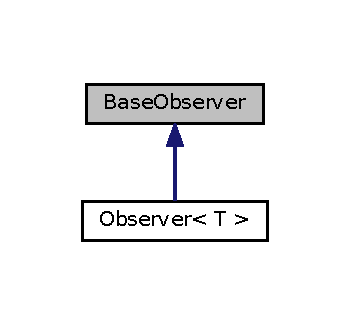
\includegraphics[width=168pt]{classKatabatic_1_1BaseObserver__inherit__graph}
\end{center}
\end{figure}
\subsection*{Public Member Functions}
\begin{DoxyCompactItemize}
\item 
virtual void \mbox{\hyperlink{classKatabatic_1_1BaseObserver_a52e577fb0c4f2e3650928334fb621c2f}{notify}} (unsigned int flags)
\end{DoxyCompactItemize}


\subsection{Detailed Description}
\mbox{\hyperlink{classKatabatic_1_1Observer}{Observer}} Design Pattern, \mbox{\hyperlink{classKatabatic_1_1Observer}{Observer}} part. 

This class is used as a non-\/template base class for the templatized \mbox{\hyperlink{classKatabatic_1_1Observer}{Observer}} one. It is used to avoid propagating template to the whole \mbox{\hyperlink{classKatabatic_1_1Observable}{Observable}} class. It only contains the \mbox{\hyperlink{classKatabatic_1_1BaseObserver_a52e577fb0c4f2e3650928334fb621c2f}{Observer\+::notify()}} virtual method. 

\subsection{Member Function Documentation}
\mbox{\Hypertarget{classKatabatic_1_1BaseObserver_a52e577fb0c4f2e3650928334fb621c2f}\label{classKatabatic_1_1BaseObserver_a52e577fb0c4f2e3650928334fb621c2f}} 
\index{Katabatic\+::\+Base\+Observer@{Katabatic\+::\+Base\+Observer}!notify@{notify}}
\index{notify@{notify}!Katabatic\+::\+Base\+Observer@{Katabatic\+::\+Base\+Observer}}
\subsubsection{\texorpdfstring{notify()}{notify()}}
{\footnotesize\ttfamily void notify (\begin{DoxyParamCaption}\item[{unsigned int}]{flags }\end{DoxyParamCaption})\hspace{0.3cm}{\ttfamily [virtual]}}

The method which will be called whenever a change occurs on the \mbox{\hyperlink{classKatabatic_1_1Observable}{Observable}}. 

Referenced by Observable\+::notify().



The documentation for this class was generated from the following files\+:\begin{DoxyCompactItemize}
\item 
Observer.\+h\item 
Observer.\+cpp\item 
Observer.\+dox\end{DoxyCompactItemize}

\hypertarget{classKatabatic_1_1ChipTools}{}\section{Chip\+Tools Class Reference}
\label{classKatabatic_1_1ChipTools}\index{Chip\+Tools@{Chip\+Tools}}


Utilities for Chip Level Design.  


\subsection*{Public Member Functions}
\begin{DoxyCompactItemize}
\item 
\mbox{\hyperlink{classKatabatic_1_1ChipTools_a5296f5ccb380869255d774b70e237686}{Chip\+Tools}} (\textbf{ Cell} $\ast$)
\item 
bool \mbox{\hyperlink{classKatabatic_1_1ChipTools_ab6b7bc2b47ead460ac00a531451dc9cf}{is\+Chip}} () const
\item 
\textbf{ Cell} $\ast$ \mbox{\hyperlink{classKatabatic_1_1ChipTools_a55a3a88610ef1af9931e634f77f2403b}{get\+Cell}} () const
\item 
\textbf{ Instance} $\ast$ \mbox{\hyperlink{classKatabatic_1_1ChipTools_a8be5c4aecbe9b97ed2eb9557b046b091}{get\+Core}} () const
\item 
const \textbf{ Box} \& \mbox{\hyperlink{classKatabatic_1_1ChipTools_ada9182cc0bcdb47b156a29cf42d08651}{get\+Chip\+Bb}} () const
\item 
const \textbf{ Box} \& \mbox{\hyperlink{classKatabatic_1_1ChipTools_aa6b5ac93ecf1ee9f94f5176664dcf4bf}{get\+Left\+Pads\+Bb}} () const
\item 
const \textbf{ Box} \& \mbox{\hyperlink{classKatabatic_1_1ChipTools_a07e88c4c6a615019e618af327829f4d0}{get\+Right\+Pads\+Bb}} () const
\item 
const \textbf{ Box} \& \mbox{\hyperlink{classKatabatic_1_1ChipTools_ad31ff1dbfdf55216d684b4032a73db6b}{get\+Top\+Pads\+Bb}} () const
\item 
const \textbf{ Box} \& \mbox{\hyperlink{classKatabatic_1_1ChipTools_aad46c56aeb14b07fcdfe93b51c554828}{get\+Bottom\+Pads\+Bb}} () const
\item 
const Torus \& \mbox{\hyperlink{classKatabatic_1_1ChipTools_a19c65013cccd38e5d4169fc25454b938}{get\+Corona}} () const
\item 
bool \mbox{\hyperlink{classKatabatic_1_1ChipTools_a708cdae658a916324059d321fafeaa7d}{intersect\+V\+Pads}} (const \textbf{ Box} \&) const
\item 
bool \mbox{\hyperlink{classKatabatic_1_1ChipTools_aeead79862ba27f1219a3cbb3ef6999d2}{intersect\+H\+Pads}} (const \textbf{ Box} \&) const
\end{DoxyCompactItemize}


\subsection{Detailed Description}
Utilities for Chip Level Design. 

The \mbox{\hyperlink{classKatabatic_1_1ChipTools}{Chip\+Tools}} class provides a small set of utilities to ease the managment of a complete chip following the Alliance top hierarchical structure. 

\subsection{Constructor \& Destructor Documentation}
\mbox{\Hypertarget{classKatabatic_1_1ChipTools_a5296f5ccb380869255d774b70e237686}\label{classKatabatic_1_1ChipTools_a5296f5ccb380869255d774b70e237686}} 
\index{Katabatic\+::\+Chip\+Tools@{Katabatic\+::\+Chip\+Tools}!Chip\+Tools@{Chip\+Tools}}
\index{Chip\+Tools@{Chip\+Tools}!Katabatic\+::\+Chip\+Tools@{Katabatic\+::\+Chip\+Tools}}
\subsubsection{\texorpdfstring{Chip\+Tools()}{ChipTools()}}
{\footnotesize\ttfamily \mbox{\hyperlink{classKatabatic_1_1ChipTools}{Chip\+Tools}} (\begin{DoxyParamCaption}\item[{\textbf{ Cell} $\ast$}]{cell }\end{DoxyParamCaption})}

Create a Chip\+Tool for {\ttfamily cell}. 

References Cell\+::get\+Abutment\+Box(), Entity\+::get\+Bounding\+Box(), Data\+Base\+::get\+D\+B(), Box\+::get\+Height(), Net\+::get\+Horizontals(), Technology\+::get\+Layer(), Instance\+::get\+Master\+Cell(), Instance\+::get\+Name(), Cell\+::get\+Name(), Cell\+::get\+Net(), Data\+Base\+::get\+Technology(), Box\+::get\+Width(), Box\+::get\+X\+Max(), Box\+::get\+X\+Min(), Box\+::get\+Y\+Max(), Box\+::get\+Y\+Min(), Box\+::inflate(), and Chip\+Tools\+::is\+Chip().



\subsection{Member Function Documentation}
\mbox{\Hypertarget{classKatabatic_1_1ChipTools_ab6b7bc2b47ead460ac00a531451dc9cf}\label{classKatabatic_1_1ChipTools_ab6b7bc2b47ead460ac00a531451dc9cf}} 
\index{Katabatic\+::\+Chip\+Tools@{Katabatic\+::\+Chip\+Tools}!is\+Chip@{is\+Chip}}
\index{is\+Chip@{is\+Chip}!Katabatic\+::\+Chip\+Tools@{Katabatic\+::\+Chip\+Tools}}
\subsubsection{\texorpdfstring{is\+Chip()}{isChip()}}
{\footnotesize\ttfamily bool is\+Chip (\begin{DoxyParamCaption}{ }\end{DoxyParamCaption}) const\hspace{0.3cm}{\ttfamily [inline]}}

{\bfseries Returns\+:} {\bfseries true} if the Cell is truly a top level design. If not, this object is useless and does nothing. 

Referenced by Chip\+Tools\+::\+Chip\+Tools(), Katabatic\+Engine\+::create\+Detailed\+Grid(), and Katabatic\+Engine\+::is\+Chip().

\mbox{\Hypertarget{classKatabatic_1_1ChipTools_a55a3a88610ef1af9931e634f77f2403b}\label{classKatabatic_1_1ChipTools_a55a3a88610ef1af9931e634f77f2403b}} 
\index{Katabatic\+::\+Chip\+Tools@{Katabatic\+::\+Chip\+Tools}!get\+Cell@{get\+Cell}}
\index{get\+Cell@{get\+Cell}!Katabatic\+::\+Chip\+Tools@{Katabatic\+::\+Chip\+Tools}}
\subsubsection{\texorpdfstring{get\+Cell()}{getCell()}}
{\footnotesize\ttfamily \textbf{ Cell} $\ast$ get\+Cell (\begin{DoxyParamCaption}{ }\end{DoxyParamCaption}) const\hspace{0.3cm}{\ttfamily [inline]}}

{\bfseries Returns\+:} The top-\/level design. \mbox{\Hypertarget{classKatabatic_1_1ChipTools_a8be5c4aecbe9b97ed2eb9557b046b091}\label{classKatabatic_1_1ChipTools_a8be5c4aecbe9b97ed2eb9557b046b091}} 
\index{Katabatic\+::\+Chip\+Tools@{Katabatic\+::\+Chip\+Tools}!get\+Core@{get\+Core}}
\index{get\+Core@{get\+Core}!Katabatic\+::\+Chip\+Tools@{Katabatic\+::\+Chip\+Tools}}
\subsubsection{\texorpdfstring{get\+Core()}{getCore()}}
{\footnotesize\ttfamily \textbf{ Instance} $\ast$ get\+Core (\begin{DoxyParamCaption}{ }\end{DoxyParamCaption}) const\hspace{0.3cm}{\ttfamily [inline]}}

{\bfseries Returns\+:} The instance of the core, that is, the only instance that is {\itshape not} a pad... \mbox{\Hypertarget{classKatabatic_1_1ChipTools_ada9182cc0bcdb47b156a29cf42d08651}\label{classKatabatic_1_1ChipTools_ada9182cc0bcdb47b156a29cf42d08651}} 
\index{Katabatic\+::\+Chip\+Tools@{Katabatic\+::\+Chip\+Tools}!get\+Chip\+Bb@{get\+Chip\+Bb}}
\index{get\+Chip\+Bb@{get\+Chip\+Bb}!Katabatic\+::\+Chip\+Tools@{Katabatic\+::\+Chip\+Tools}}
\subsubsection{\texorpdfstring{get\+Chip\+Bb()}{getChipBb()}}
{\footnotesize\ttfamily const \textbf{ Box} \& get\+Chip\+Bb (\begin{DoxyParamCaption}{ }\end{DoxyParamCaption}) const\hspace{0.3cm}{\ttfamily [inline]}}

{\bfseries Returns\+:} The chip complete bounding box, this $\ast$is$\ast$ simply the Cell bounding box. \mbox{\Hypertarget{classKatabatic_1_1ChipTools_aa6b5ac93ecf1ee9f94f5176664dcf4bf}\label{classKatabatic_1_1ChipTools_aa6b5ac93ecf1ee9f94f5176664dcf4bf}} 
\index{Katabatic\+::\+Chip\+Tools@{Katabatic\+::\+Chip\+Tools}!get\+Left\+Pads\+Bb@{get\+Left\+Pads\+Bb}}
\index{get\+Left\+Pads\+Bb@{get\+Left\+Pads\+Bb}!Katabatic\+::\+Chip\+Tools@{Katabatic\+::\+Chip\+Tools}}
\subsubsection{\texorpdfstring{get\+Left\+Pads\+Bb()}{getLeftPadsBb()}}
{\footnotesize\ttfamily const \textbf{ Box} \& get\+Left\+Pads\+Bb (\begin{DoxyParamCaption}{ }\end{DoxyParamCaption}) const\hspace{0.3cm}{\ttfamily [inline]}}

{\bfseries Returns\+:} The bounding box enclosing all the pads on the left side of the chip.

\begin{DoxyParagraph}{Remark\+: This box is computed from the chip bounding box and the pad height. }

\end{DoxyParagraph}
\mbox{\Hypertarget{classKatabatic_1_1ChipTools_a07e88c4c6a615019e618af327829f4d0}\label{classKatabatic_1_1ChipTools_a07e88c4c6a615019e618af327829f4d0}} 
\index{Katabatic\+::\+Chip\+Tools@{Katabatic\+::\+Chip\+Tools}!get\+Right\+Pads\+Bb@{get\+Right\+Pads\+Bb}}
\index{get\+Right\+Pads\+Bb@{get\+Right\+Pads\+Bb}!Katabatic\+::\+Chip\+Tools@{Katabatic\+::\+Chip\+Tools}}
\subsubsection{\texorpdfstring{get\+Right\+Pads\+Bb()}{getRightPadsBb()}}
{\footnotesize\ttfamily const \textbf{ Box} \& get\+Right\+Pads\+Bb (\begin{DoxyParamCaption}{ }\end{DoxyParamCaption}) const\hspace{0.3cm}{\ttfamily [inline]}}

{\bfseries Returns\+:} The bounding box enclosing all the pads on the right side of the chip.

\begin{DoxyParagraph}{Remark\+: This box is computed from the chip bounding box and the pad height. }

\end{DoxyParagraph}
\mbox{\Hypertarget{classKatabatic_1_1ChipTools_ad31ff1dbfdf55216d684b4032a73db6b}\label{classKatabatic_1_1ChipTools_ad31ff1dbfdf55216d684b4032a73db6b}} 
\index{Katabatic\+::\+Chip\+Tools@{Katabatic\+::\+Chip\+Tools}!get\+Top\+Pads\+Bb@{get\+Top\+Pads\+Bb}}
\index{get\+Top\+Pads\+Bb@{get\+Top\+Pads\+Bb}!Katabatic\+::\+Chip\+Tools@{Katabatic\+::\+Chip\+Tools}}
\subsubsection{\texorpdfstring{get\+Top\+Pads\+Bb()}{getTopPadsBb()}}
{\footnotesize\ttfamily const \textbf{ Box} \& get\+Top\+Pads\+Bb (\begin{DoxyParamCaption}{ }\end{DoxyParamCaption}) const\hspace{0.3cm}{\ttfamily [inline]}}

{\bfseries Returns\+:} The bounding box enclosing all the pads on the top side of the chip.

\begin{DoxyParagraph}{Remark\+: This box is computed from the chip bounding box and the pad height. }

\end{DoxyParagraph}
\mbox{\Hypertarget{classKatabatic_1_1ChipTools_aad46c56aeb14b07fcdfe93b51c554828}\label{classKatabatic_1_1ChipTools_aad46c56aeb14b07fcdfe93b51c554828}} 
\index{Katabatic\+::\+Chip\+Tools@{Katabatic\+::\+Chip\+Tools}!get\+Bottom\+Pads\+Bb@{get\+Bottom\+Pads\+Bb}}
\index{get\+Bottom\+Pads\+Bb@{get\+Bottom\+Pads\+Bb}!Katabatic\+::\+Chip\+Tools@{Katabatic\+::\+Chip\+Tools}}
\subsubsection{\texorpdfstring{get\+Bottom\+Pads\+Bb()}{getBottomPadsBb()}}
{\footnotesize\ttfamily const \textbf{ Box} \& get\+Bottom\+Pads\+Bb (\begin{DoxyParamCaption}{ }\end{DoxyParamCaption}) const\hspace{0.3cm}{\ttfamily [inline]}}

{\bfseries Returns\+:} The bounding box enclosing all the pads on the bottom side of the chip.

\begin{DoxyParagraph}{Remark\+: This box is computed from the chip bounding box and the pad height. }

\end{DoxyParagraph}
\mbox{\Hypertarget{classKatabatic_1_1ChipTools_a19c65013cccd38e5d4169fc25454b938}\label{classKatabatic_1_1ChipTools_a19c65013cccd38e5d4169fc25454b938}} 
\index{Katabatic\+::\+Chip\+Tools@{Katabatic\+::\+Chip\+Tools}!get\+Corona@{get\+Corona}}
\index{get\+Corona@{get\+Corona}!Katabatic\+::\+Chip\+Tools@{Katabatic\+::\+Chip\+Tools}}
\subsubsection{\texorpdfstring{get\+Corona()}{getCorona()}}
{\footnotesize\ttfamily const Torus \& get\+Corona (\begin{DoxyParamCaption}{ }\end{DoxyParamCaption}) const\hspace{0.3cm}{\ttfamily [inline]}}

{\bfseries Returns\+:} The torus (in term of manhanttan distance) enclosed between the pad area and the core area. \mbox{\Hypertarget{classKatabatic_1_1ChipTools_a708cdae658a916324059d321fafeaa7d}\label{classKatabatic_1_1ChipTools_a708cdae658a916324059d321fafeaa7d}} 
\index{Katabatic\+::\+Chip\+Tools@{Katabatic\+::\+Chip\+Tools}!intersect\+V\+Pads@{intersect\+V\+Pads}}
\index{intersect\+V\+Pads@{intersect\+V\+Pads}!Katabatic\+::\+Chip\+Tools@{Katabatic\+::\+Chip\+Tools}}
\subsubsection{\texorpdfstring{intersect\+V\+Pads()}{intersectVPads()}}
{\footnotesize\ttfamily bool intersect\+V\+Pads (\begin{DoxyParamCaption}\item[{const \textbf{ Box} \&}]{box }\end{DoxyParamCaption}) const\hspace{0.3cm}{\ttfamily [inline]}}

{\bfseries Returns\+:} {\bfseries true} if {\ttfamily box} intersect either the left or right pad box. 

References Box\+::intersect().

\mbox{\Hypertarget{classKatabatic_1_1ChipTools_aeead79862ba27f1219a3cbb3ef6999d2}\label{classKatabatic_1_1ChipTools_aeead79862ba27f1219a3cbb3ef6999d2}} 
\index{Katabatic\+::\+Chip\+Tools@{Katabatic\+::\+Chip\+Tools}!intersect\+H\+Pads@{intersect\+H\+Pads}}
\index{intersect\+H\+Pads@{intersect\+H\+Pads}!Katabatic\+::\+Chip\+Tools@{Katabatic\+::\+Chip\+Tools}}
\subsubsection{\texorpdfstring{intersect\+H\+Pads()}{intersectHPads()}}
{\footnotesize\ttfamily bool intersect\+H\+Pads (\begin{DoxyParamCaption}\item[{const \textbf{ Box} \&}]{box }\end{DoxyParamCaption}) const\hspace{0.3cm}{\ttfamily [inline]}}

{\bfseries Returns\+:} {\bfseries true} if {\ttfamily box} intersect either the top or bottom pad box. 

References Box\+::intersect().



The documentation for this class was generated from the following files\+:\begin{DoxyCompactItemize}
\item 
Chip\+Tools.\+h\item 
Chip\+Tools.\+cpp\item 
Chip\+Tools.\+dox\end{DoxyCompactItemize}

\hypertarget{classKatabatic_1_1GCell_1_1CompareByDensity}{}\section{G\+Cell\+:\+:Compare\+By\+Density Class Reference}
\label{classKatabatic_1_1GCell_1_1CompareByDensity}\index{G\+Cell\+::\+Compare\+By\+Density@{G\+Cell\+::\+Compare\+By\+Density}}


\mbox{\hyperlink{classKatabatic_1_1GCell}{G\+Cell}} Density Comparison Functor.  




Inherits binary\+\_\+function$<$ G\+Cell $\ast$, G\+Cell $\ast$, bool $>$.

\subsection*{Public Member Functions}
\begin{DoxyCompactItemize}
\item 
\mbox{\hyperlink{classKatabatic_1_1GCell_1_1CompareByDensity_a3a51c3a473276097f23c5f58c6800f9b}{Compare\+By\+Density}} (unsigned int depth)
\end{DoxyCompactItemize}


\subsection{Detailed Description}
\mbox{\hyperlink{classKatabatic_1_1GCell}{G\+Cell}} Density Comparison Functor. 

A comparison functor for \mbox{\hyperlink{classKatabatic_1_1GCell}{G\+Cell}}, compare by density on layer {\ttfamily depth}. 

\subsection{Constructor \& Destructor Documentation}
\mbox{\Hypertarget{classKatabatic_1_1GCell_1_1CompareByDensity_a3a51c3a473276097f23c5f58c6800f9b}\label{classKatabatic_1_1GCell_1_1CompareByDensity_a3a51c3a473276097f23c5f58c6800f9b}} 
\index{Katabatic\+::\+G\+Cell\+::\+Compare\+By\+Density@{Katabatic\+::\+G\+Cell\+::\+Compare\+By\+Density}!Compare\+By\+Density@{Compare\+By\+Density}}
\index{Compare\+By\+Density@{Compare\+By\+Density}!Katabatic\+::\+G\+Cell\+::\+Compare\+By\+Density@{Katabatic\+::\+G\+Cell\+::\+Compare\+By\+Density}}
\subsubsection{\texorpdfstring{Compare\+By\+Density()}{CompareByDensity()}}
{\footnotesize\ttfamily \mbox{\hyperlink{classKatabatic_1_1GCell_1_1CompareByDensity}{Compare\+By\+Density}} (\begin{DoxyParamCaption}\item[{unsigned int}]{depth }\end{DoxyParamCaption})}

Build a density comparator for G\+Cells on layer {\ttfamily depth}. 

The documentation for this class was generated from the following files\+:\begin{DoxyCompactItemize}
\item 
G\+Cell.\+h\item 
G\+Cell.\+cpp\item 
G\+Cell.\+dox\end{DoxyCompactItemize}

\hypertarget{classKatabatic_1_1GCell_1_1CompareByIndex}{}\section{G\+Cell\+:\+:Compare\+By\+Index Class Reference}
\label{classKatabatic_1_1GCell_1_1CompareByIndex}\index{G\+Cell\+::\+Compare\+By\+Index@{G\+Cell\+::\+Compare\+By\+Index}}


\mbox{\hyperlink{classKatabatic_1_1GCell}{G\+Cell}} Index Comparison Functor.  




Inherits binary\+\_\+function$<$ const G\+Cell $\ast$, const G\+Cell $\ast$, bool $>$.



\subsection{Detailed Description}
\mbox{\hyperlink{classKatabatic_1_1GCell}{G\+Cell}} Index Comparison Functor. 

A comparison functor for \mbox{\hyperlink{classKatabatic_1_1GCell}{G\+Cell}}, compare by {\ttfamily index} (the linear index in the \mbox{\hyperlink{classKatabatic_1_1GCellGrid}{G\+Cell\+Grid}} vector. 

The documentation for this class was generated from the following file\+:\begin{DoxyCompactItemize}
\item 
G\+Cell.\+h\end{DoxyCompactItemize}

\hypertarget{classKatabatic_1_1GCell}{}\section{G\+Cell Class Reference}
\label{classKatabatic_1_1GCell}\index{G\+Cell@{G\+Cell}}


Routing Global Cell.  




Inherits Extension\+Go.

\subsection*{Classes}
\begin{DoxyCompactItemize}
\item 
class \mbox{\hyperlink{classKatabatic_1_1GCell_1_1CompareByDensity}{Compare\+By\+Density}}
\begin{DoxyCompactList}\small\item\em \mbox{\hyperlink{classKatabatic_1_1GCell}{G\+Cell}} Density Comparison Functor. \end{DoxyCompactList}\item 
class \mbox{\hyperlink{classKatabatic_1_1GCell_1_1CompareByIndex}{Compare\+By\+Index}}
\begin{DoxyCompactList}\small\item\em \mbox{\hyperlink{classKatabatic_1_1GCell}{G\+Cell}} Index Comparison Functor. \end{DoxyCompactList}\item 
class \mbox{\hyperlink{classKatabatic_1_1GCell_1_1Key}{Key}}
\begin{DoxyCompactList}\small\item\em \mbox{\hyperlink{classKatabatic_1_1GCell}{G\+Cell}} \mbox{\hyperlink{classKatabatic_1_1GCell_1_1Key}{Key}} -\/ Density Cache. \end{DoxyCompactList}\end{DoxyCompactItemize}
\subsection*{Public Types}
\begin{DoxyCompactItemize}
\item 
typedef set$<$ \mbox{\hyperlink{classKatabatic_1_1GCell}{G\+Cell}} $\ast$, \mbox{\hyperlink{classKatabatic_1_1GCell_1_1CompareByIndex}{Compare\+By\+Index}} $>$ \mbox{\hyperlink{classKatabatic_1_1GCell_aacb1c215b203bfba5729f135b3221d40}{Set\+Index}}
\end{DoxyCompactItemize}
\subsection*{Public Member Functions}
\begin{DoxyCompactItemize}
\item 
virtual const \textbf{ Name} \& \mbox{\hyperlink{classKatabatic_1_1GCell_a9e76ae5cee9320b65251387419c9432b}{get\+Name}} () const
\item 
bool \mbox{\hyperlink{classKatabatic_1_1GCell_a9f274f17cf9166e997d306b120618fdf}{is\+Saturated}} () const
\item 
bool \mbox{\hyperlink{classKatabatic_1_1GCell_a49b7bd2f05abd94436177558fd0f97d8}{is\+Saturated}} (unsigned int depth) const
\item 
bool \mbox{\hyperlink{classKatabatic_1_1GCell_a5bc2a781be2586924afce4e4a4ea6697}{is\+Valid}} () const
\item 
bool \mbox{\hyperlink{classKatabatic_1_1GCell_a0e0a7b382b06e230051965bcb78ed21c}{is\+Above\+Density}} (float threshold) const
\item 
bool \mbox{\hyperlink{classKatabatic_1_1GCell_ac2275a015db51cc12dd53fb13d22ca4f}{has\+Free\+Track}} (size\+\_\+t depth, float reserve) const
\item 
\mbox{\hyperlink{classKatabatic_1_1GCellGrid}{G\+Cell\+Grid}} $\ast$ \mbox{\hyperlink{classKatabatic_1_1GCell_a9a56286f633fddd702d66563de457a4a}{get\+G\+Cell\+Grid}} () const
\item 
unsigned int \mbox{\hyperlink{classKatabatic_1_1GCell_a6c4d9081746b8daa3e45e5e3dd185b60}{get\+Depth}} () const
\item 
unsigned int \mbox{\hyperlink{classKatabatic_1_1GCell_a762de91e7869ca544ff034b99fc2e0a6}{get\+Index}} () const
\item 
unsigned int \mbox{\hyperlink{classKatabatic_1_1GCell_ad26f8bcf642c2620ac525cc04c8376c0}{get\+Row}} () const
\item 
unsigned int \mbox{\hyperlink{classKatabatic_1_1GCell_ac5b1a776c3eafa7f68d31292615011fa}{get\+Column}} () const
\item 
\mbox{\hyperlink{classKatabatic_1_1GCell}{G\+Cell}} $\ast$ \mbox{\hyperlink{classKatabatic_1_1GCell_a633722329744550b6da94c3b6fb97484}{get\+Left}} () const
\item 
\mbox{\hyperlink{classKatabatic_1_1GCell}{G\+Cell}} $\ast$ \mbox{\hyperlink{classKatabatic_1_1GCell_abdeb6b4a351f8b292894d3f0c24f105d}{get\+Right}} () const
\item 
\mbox{\hyperlink{classKatabatic_1_1GCell}{G\+Cell}} $\ast$ \mbox{\hyperlink{classKatabatic_1_1GCell_a335506a314a2330b5a354906e798e60c}{get\+Up}} () const
\item 
\mbox{\hyperlink{classKatabatic_1_1GCell}{G\+Cell}} $\ast$ \mbox{\hyperlink{classKatabatic_1_1GCell_ae448c9d6d028e967d7bd5a1bfdd05311}{get\+Down}} () const
\item 
virtual void \mbox{\hyperlink{classKatabatic_1_1GCell_a819f3ffbba69e4de2a19c827676b5aee}{translate}} (const \textbf{ Db\+U\+::\+Unit} \&, const \textbf{ Db\+U\+::\+Unit} \&)
\item 
virtual \textbf{ Box} \mbox{\hyperlink{classKatabatic_1_1GCell_ab5d8bf98ab5af6fcfebea1b9f446d5d7}{get\+Bounding\+Box}} () const
\item 
\textbf{ Db\+U\+::\+Unit} \mbox{\hyperlink{classKatabatic_1_1GCell_a00b8f54c8171f6699e57de1b8c18eeb1}{getX}} () const
\item 
\textbf{ Db\+U\+::\+Unit} \mbox{\hyperlink{classKatabatic_1_1GCell_a4580de6b074712e400d5d238ce3af054}{getY}} () const
\item 
\textbf{ Db\+U\+::\+Unit} \mbox{\hyperlink{classKatabatic_1_1GCell_aaf7ff16cd2fd5a3fa4c5221efb9b9b76}{get\+X\+Max}} () const
\item 
\textbf{ Db\+U\+::\+Unit} \mbox{\hyperlink{classKatabatic_1_1GCell_a096a92c18156eac4268efb50496a2d18}{get\+Y\+Max}} () const
\item 
\textbf{ Interval} \mbox{\hyperlink{classKatabatic_1_1GCell_a10f3dd5001b2015e34a9aacdacf6eae6}{get\+Side}} (unsigned int) const
\item 
float \mbox{\hyperlink{classKatabatic_1_1GCell_ad0dda8d59162b90040263fc55d7da714}{get\+H\+Capacity}} () const
\item 
float \mbox{\hyperlink{classKatabatic_1_1GCell_a3994e204ebccf8aa12899e0c5ef4112b}{get\+V\+Capacity}} () const
\item 
float \mbox{\hyperlink{classKatabatic_1_1GCell_ad31c16c87377e164728a0df55e21f96b}{get\+Density}} (unsigned int flags=0) const
\item 
float \mbox{\hyperlink{classKatabatic_1_1GCell_ae56b981fad5960835faef809ec282cfa}{get\+C\+Density}} (unsigned int flags=0) const
\item 
float \mbox{\hyperlink{classKatabatic_1_1GCell_aa64538731e911c60eeaea557be1c7740}{get\+W\+Density}} (unsigned int depth, unsigned int flags=0) const
\item 
\textbf{ Db\+U\+::\+Unit} \mbox{\hyperlink{classKatabatic_1_1GCell_ab37ffda5a2e1ba60931d32c29237bd33}{get\+Blockage}} (unsigned int depth) const
\item 
float \mbox{\hyperlink{classKatabatic_1_1GCell_a44ec8d16030b5900bd0ccc02652b727f}{get\+Fragmentation}} (unsigned int depth) const
\item 
float \mbox{\hyperlink{classKatabatic_1_1GCell_a14feed45699c8dc406251519dc08bc79}{get\+Feedthroughs}} (unsigned int depth) const
\item 
float \mbox{\hyperlink{classKatabatic_1_1GCell_a4785bcc49da76fc38f6940f5b1cc5b17}{get\+Globals\+Count}} (unsigned int depth) const
\item 
const vector$<$ \mbox{\hyperlink{classKatabatic_1_1AutoSegment}{Auto\+Segment}} $\ast$ $>$ \& \mbox{\hyperlink{classKatabatic_1_1GCell_a81575302a8794958c310dc101807e9c5}{get\+H\+Segments}} () const
\item 
const vector$<$ \mbox{\hyperlink{classKatabatic_1_1AutoSegment}{Auto\+Segment}} $\ast$ $>$ \& \mbox{\hyperlink{classKatabatic_1_1GCell_ac3c357d72a24990494758dcc216e3b1e}{get\+V\+Segments}} () const
\item 
const vector$<$ \mbox{\hyperlink{classKatabatic_1_1AutoContact}{Auto\+Contact}} $\ast$ $>$ \& \mbox{\hyperlink{classKatabatic_1_1GCell_aacf50ce6dcef3a7523453725af7feeae}{get\+Contacts}} () const
\item 
\mbox{\hyperlink{namespaceKatabatic_a2221b0ddbc24f331809fc86f98e38041}{Auto\+Segments}} \mbox{\hyperlink{classKatabatic_1_1GCell_a79668a41675e9ba0ca59d4b91e3b70be}{get\+H\+Start\+Segments}} ()
\item 
\mbox{\hyperlink{namespaceKatabatic_a2221b0ddbc24f331809fc86f98e38041}{Auto\+Segments}} \mbox{\hyperlink{classKatabatic_1_1GCell_acbd17a4441905a4f5bc33a26bb338d0a}{get\+V\+Start\+Segments}} ()
\item 
\mbox{\hyperlink{namespaceKatabatic_a2221b0ddbc24f331809fc86f98e38041}{Auto\+Segments}} \mbox{\hyperlink{classKatabatic_1_1GCell_a77beccf65527a330f15bed2aba4f9dea}{get\+H\+Stop\+Segments}} ()
\item 
\mbox{\hyperlink{namespaceKatabatic_a2221b0ddbc24f331809fc86f98e38041}{Auto\+Segments}} \mbox{\hyperlink{classKatabatic_1_1GCell_a2f0f038f5700b7b55f22829c5d43aa07}{get\+V\+Stop\+Segments}} ()
\item 
\mbox{\hyperlink{namespaceKatabatic_a2221b0ddbc24f331809fc86f98e38041}{Auto\+Segments}} \mbox{\hyperlink{classKatabatic_1_1GCell_a1f92568d22b1384a8cdf328340fb9160}{get\+Start\+Segments}} (unsigned int direction)
\item 
\mbox{\hyperlink{namespaceKatabatic_a2221b0ddbc24f331809fc86f98e38041}{Auto\+Segments}} \mbox{\hyperlink{classKatabatic_1_1GCell_a80ad0f9e79bccf6aed4fb69b4b795005}{get\+Stop\+Segments}} (unsigned int direction)
\item 
size\+\_\+t \mbox{\hyperlink{classKatabatic_1_1GCell_a3bda8c3dbb2896a0e6e57f974d0c1cad}{get\+Routing\+Pads}} (set$<$ \textbf{ Routing\+Pad} $\ast$$>$ \&)
\item 
const \mbox{\hyperlink{classKatabatic_1_1GCell_1_1Key}{Key}} \& \mbox{\hyperlink{classKatabatic_1_1GCell_ade1e79e88bf4f4c173ffd083dd5470c9}{get\+Key}} () const
\item 
size\+\_\+t \mbox{\hyperlink{classKatabatic_1_1GCell_a88208864ba2268689946a8cb7a86fcb2}{check\+Density}} () const
\item 
bool \mbox{\hyperlink{classKatabatic_1_1GCell_af4dcc99733b7ea77e8c3c7da9ac3cd3c}{check\+Edge\+Saturation}} (size\+\_\+t hreserved, size\+\_\+t vreserved) const
\item 
void \mbox{\hyperlink{classKatabatic_1_1GCell_a1270eab34ac57f21c0286a5455044a0d}{add\+Blockage}} (unsigned int depth, \textbf{ Db\+U\+::\+Unit})
\item 
void \mbox{\hyperlink{classKatabatic_1_1GCell_a4aad7d6f7357fd7963aab91bc2019a1b}{add\+H\+Segment}} (\mbox{\hyperlink{classKatabatic_1_1AutoSegment}{Auto\+Segment}} $\ast$)
\item 
void \mbox{\hyperlink{classKatabatic_1_1GCell_a8aa815e9e99df8187e628f6ec9e9da77}{add\+V\+Segment}} (\mbox{\hyperlink{classKatabatic_1_1AutoSegment}{Auto\+Segment}} $\ast$)
\item 
void \mbox{\hyperlink{classKatabatic_1_1GCell_a2b84aab620bfca1064e988e94e7b9c59}{add\+Contact}} (\mbox{\hyperlink{classKatabatic_1_1AutoContact}{Auto\+Contact}} $\ast$)
\item 
void \mbox{\hyperlink{classKatabatic_1_1GCell_abe128484d8aa063198292a88c63f2bba}{remove\+V\+Segment}} (\mbox{\hyperlink{classKatabatic_1_1AutoSegment}{Auto\+Segment}} $\ast$)
\item 
void \mbox{\hyperlink{classKatabatic_1_1GCell_aff76aa96214c0efcf13186b8b3e5c852}{remove\+H\+Segment}} (\mbox{\hyperlink{classKatabatic_1_1AutoSegment}{Auto\+Segment}} $\ast$)
\item 
void \mbox{\hyperlink{classKatabatic_1_1GCell_aa052a9427fbd4185f00567a97770f80b}{remove\+Contact}} (\mbox{\hyperlink{classKatabatic_1_1AutoContact}{Auto\+Contact}} $\ast$)
\item 
void \mbox{\hyperlink{classKatabatic_1_1GCell_aa0beea2ceaa543503346967085036d1a}{update\+Contacts}} ()
\item 
size\+\_\+t \mbox{\hyperlink{classKatabatic_1_1GCell_a9b3455dce10eb98d0496175dd586528c}{update\+Density}} ()
\item 
void \mbox{\hyperlink{classKatabatic_1_1GCell_a11beff0f0bec06d0f3e080969516dfc3}{update\+Key}} (unsigned int depth)
\item 
void \mbox{\hyperlink{classKatabatic_1_1GCell_a11f07f57cc33fcd4b2d310145c778801}{rp\+Desaturate}} (set$<$ \textbf{ Net} $\ast$$>$ \&)
\item 
bool \mbox{\hyperlink{classKatabatic_1_1GCell_a5ae4d250ebecf59aa98fb068d848be14}{step\+Desaturate}} (unsigned int depth, set$<$ \textbf{ Net} $\ast$$>$ \&, \mbox{\hyperlink{classKatabatic_1_1AutoSegment}{Auto\+Segment}} $\ast$\&moved, unsigned int flags=0)
\item 
bool \mbox{\hyperlink{classKatabatic_1_1GCell_abe4cf4a81bb78e9b479992336a999a07}{step\+Net\+Desaturate}} (unsigned int depth, set$<$ \textbf{ Net} $\ast$$>$ \&global\+Nets, \mbox{\hyperlink{classKatabatic_1_1GCell_aacb1c215b203bfba5729f135b3221d40}{Set\+Index}} \&invalidateds)
\end{DoxyCompactItemize}
\subsection*{Static Public Member Functions}
\begin{DoxyCompactItemize}
\item 
static size\+\_\+t \mbox{\hyperlink{classKatabatic_1_1GCell_a91c8bc1a6bdb1b15c3c084ebfd38af47}{get\+Allocateds}} ()
\item 
static \textbf{ Db\+U\+::\+Unit} \mbox{\hyperlink{classKatabatic_1_1GCell_ac594cb2832ee7ef410c89499258d38fd}{get\+Top\+Right\+Shrink}} ()
\item 
static const \textbf{ Name} \& \mbox{\hyperlink{classKatabatic_1_1GCell_a00e56270cfb31f56e52e31afbc33ba71}{get\+Static\+Name}} ()
\end{DoxyCompactItemize}


\subsection{Detailed Description}
Routing Global Cell. 

\hypertarget{classKatabatic_1_1GCell_secGCellDescription}{}\subsection{G\+Cell Description}\label{classKatabatic_1_1GCell_secGCellDescription}
Please note that there are two kind of Global Cells (or \mbox{\hyperlink{classKatabatic_1_1GCell}{G\+Cell}} for short)\+:
\begin{DoxyItemize}
\item The \mbox{\hyperlink{classKatabatic_1_1GCell}{G\+Cell}} used by the global router Knik.
\item The \mbox{\hyperlink{classKatabatic_1_1GCell}{G\+Cell}} used by the detailed router (\mbox{\hyperlink{namespaceKatabatic}{Katabatic}} \& Kite). Although the information they hold is obviously related, they are two separate kind of objects.
\end{DoxyItemize}

The area of the design to be routed is divided in a regular grid of rectangular area, the \mbox{\hyperlink{classKatabatic_1_1GCellGrid}{G\+Cell\+Grid}}. Each rectangular area is a \mbox{\hyperlink{classKatabatic_1_1GCell}{G\+Cell}}.

The \mbox{\hyperlink{classKatabatic_1_1GCell}{G\+Cell}} contains the following informations\+:
\begin{DoxyItemize}
\item The Auto\+Segments that begins or ends in it. The list of segments is not avalaible directly but through the Auto\+Contacts that are owned by the \mbox{\hyperlink{classKatabatic_1_1GCell}{G\+Cell}}.
\item The Auto\+Segments that go straight {\itshape through} it (or {\itshape over} it). Horizontal \& Vertical segments are stored in two separeted list. Those two lists are sorted by layer depth (the deepest layers first).
\item A lot of synthetic information about the density of tracks used in the \mbox{\hyperlink{classKatabatic_1_1GCell}{G\+Cell}}.
\end{DoxyItemize}

Auto\+Contacts are affected to G\+Cells, the area of the \mbox{\hyperlink{classKatabatic_1_1GCell}{G\+Cell}} is the one into which the \mbox{\hyperlink{classKatabatic_1_1AutoContact}{Auto\+Contact}} is allowed to be placed. It is this that way that the respect of the global routing choosen by Knik is enforced. See the \mbox{\hyperlink{classKatabatic_1_1AutoContact}{Auto\+Contact}} constraint box.

When tracks are aligned with the \mbox{\hyperlink{classKatabatic_1_1GCell}{G\+Cell}} boundaries they one exactly on the boundary can belong to the \mbox{\hyperlink{classKatabatic_1_1GCell}{G\+Cell}} on either side of the boundary. But we want a clear and mutually exclusive ownership of each \mbox{\hyperlink{classKatabatic_1_1GCell}{G\+Cell}} area. So, we choose that one \mbox{\hyperlink{classKatabatic_1_1GCell}{G\+Cell}} do not own the topmost and rightmost track. And to implement it, we shrink top and right coordinates by the amount of \mbox{\hyperlink{classKatabatic_1_1GCell_ac594cb2832ee7ef410c89499258d38fd}{G\+Cell\+::get\+Top\+Right\+Shrink()}}, which must be less than the track spacing.\hypertarget{classKatabatic_1_1GCell_secGCellDensity}{}\subsubsection{Saturation \& Density Computation}\label{classKatabatic_1_1GCell_secGCellDensity}
At any depth (i.\+e. layer), in the preferred routing direction, a \mbox{\hyperlink{classKatabatic_1_1GCell}{G\+Cell}} can pass a finite length of wire. For example on an horizontal preferred layer\+: \[ WL_{max} = width(GCell) \times Htracks(GCell) \] Then the density, is the ratio between $WL_{max}$ and the actually used wirelength\+: \[ Wdensity(depth) = \frac{WL_{used}(depth)}{WL_{max}(depth)} \] Normally, the ratio musn\textquotesingle{}t exceed 1.\+0, but the occupied wire length computation, for now, doesn\textquotesingle{}t merge overlapping wires belonging to the same net, so the ratio may be slightly inaccurate. Thus in some pathological cases may be greater than 1.\+0 whithout truly been overloaded.

A Cell is considered as {\itshape saturated} if the overall density is above the saturation ratio given by \mbox{\hyperlink{classKatabatic_1_1Session_a266a4079ca235e8fdb622ef4996d324d}{Session\+::get\+Saturate\+Ratio()}}.

Contact density is calculated as follow\+: \[ Cont_{density} = \frac{|Contacts|}{Htracks \times Vtracks \times 4} \] It is a ratio over the number of actual contacts in the \mbox{\hyperlink{classKatabatic_1_1GCell}{G\+Cell}} and the maximal number. The maximal number being the product of the number of tracks in both direction and 4 stands for the hardwired number of layers (the depth).

Should not be hardwired... {\itshape To be corrected in future versions.}\hypertarget{classKatabatic_1_1GCell_secGCellFeedthrough}{}\subsubsection{Feedthrough Computation}\label{classKatabatic_1_1GCell_secGCellFeedthrough}
The feedtrough value is an estimate is of how many complete tracks have been used on a given layer of the \mbox{\hyperlink{classKatabatic_1_1GCell}{G\+Cell}}. It varies between zero and the number of track on the \mbox{\hyperlink{classKatabatic_1_1GCell}{G\+Cell}} (complete saturation). As an estimate, it doesn\textquotesingle{}t tell you the actual number of free track, but how many you {\itshape may expect} assuming the routing is reasonably well done.

Computation is done as follow\+: \tabulinesep=1mm
\begin{longtabu} spread 0pt [c]{*{2}{|X[-1]}|}
\hline
\rowcolor{\tableheadbgcolor}\textbf{ Wire type}&\textbf{ Estimated Cost }\\\cline{1-2}
\endfirsthead
\hline
\endfoot
\hline
\rowcolor{\tableheadbgcolor}\textbf{ Wire type}&\textbf{ Estimated Cost }\\\cline{1-2}
\endhead
Straight wire (feedthrough) &{\bfseries 1.\+0} \\\cline{1-2}
Beginning or ending global wire &{\bfseries 0.\+5} \\\cline{1-2}
Local wire. &{\bfseries 1/3} \\\cline{1-2}
Blockage wire &The exact percentage of the track \\\cline{1-2}
\end{longtabu}
\hypertarget{classKatabatic_1_1GCell_secGCellTrackComputation}{}\subsubsection{Track Computation}\label{classKatabatic_1_1GCell_secGCellTrackComputation}
The number of track that can go through a \mbox{\hyperlink{classKatabatic_1_1GCell}{G\+Cell}} in the horizontal direction is computed as follow\+: \[ Htracks = \frac{heigth(GCell)}{Vpitch} + 1 \]

The pitch is assumed to be the same for every layer and is hardwired to 5.\+0 lambda.

This is a bad architectural choice. The informations pertaining to routing should be held at Kite level, not be hardwired and the pitch should be made variable with the layer... {\itshape To be corrected in future versions}.\hypertarget{classKatabatic_1_1GCell_secGCellLazyEvaluation}{}\subsection{G\+Cell Lazy Evaluation}\label{classKatabatic_1_1GCell_secGCellLazyEvaluation}
To save processing time, the densities are not recomputed every time a segment is modified (added, removed or moved). Instead a lazy evaluation mechanism is used. Densities are recomputed each time a density is queried {\itshape and} the lazy evaluation {\itshape not} explicitly disabled (flag No\+Update).\hypertarget{classKatabatic_1_1GCell_secGCellSortingKey}{}\subsection{G\+Cell Sorting Key}\label{classKatabatic_1_1GCell_secGCellSortingKey}
In order to perform a lexicographical sort on the tuple $(density(depth),id)$ of a \mbox{\hyperlink{classKatabatic_1_1GCell}{G\+Cell}}, a specific slave object \mbox{\hyperlink{classKatabatic_1_1GCell_1_1Key}{G\+Cell\+::\+Key}} is introduced. It is the density on one specific depth, not the average density.\hypertarget{classKatabatic_1_1GCell_secGCellDesaturation}{}\subsection{G\+Cell Desaturation / Layer Assignment}\label{classKatabatic_1_1GCell_secGCellDesaturation}
In addition to it\textquotesingle{}s geometrical and density functionality, the \mbox{\hyperlink{classKatabatic_1_1GCell}{G\+Cell}} provides {\itshape desaturation} capabilities. Desaturation is the operation of moving up feedthough \mbox{\hyperlink{classKatabatic_1_1AutoSegment}{Auto\+Segment}} from the bottom layers towards the upper ones in order to balance the densities in the different densities. Thoses operations provides building blocks for the layer assignment stage which is provided by the Kabatic tool.

Two strategies are avalaibles, moving one global \mbox{\hyperlink{classKatabatic_1_1AutoSegment}{Auto\+Segment}} at a time with \mbox{\hyperlink{classKatabatic_1_1GCell_a5ae4d250ebecf59aa98fb068d848be14}{G\+Cell\+::step\+Desaturate()}} or, when one \mbox{\hyperlink{classKatabatic_1_1AutoSegment}{Auto\+Segment}} is moved up, move up the whole net trunk with \mbox{\hyperlink{classKatabatic_1_1GCell_abe4cf4a81bb78e9b479992336a999a07}{G\+Cell\+::step\+Net\+Desaturate()}}.\hypertarget{classKatabatic_1_1GCell_secGCellImplantation}{}\subsection{G\+Cell Implantation}\label{classKatabatic_1_1GCell_secGCellImplantation}
\mbox{\hyperlink{classKatabatic_1_1GCell}{G\+Cell}} derives from Hurricane\+::\+Extension\+Go to allow a graphical rendering of the routing density. 

\subsection{Member Typedef Documentation}
\mbox{\Hypertarget{classKatabatic_1_1GCell_aacb1c215b203bfba5729f135b3221d40}\label{classKatabatic_1_1GCell_aacb1c215b203bfba5729f135b3221d40}} 
\index{Katabatic\+::\+G\+Cell@{Katabatic\+::\+G\+Cell}!Set\+Index@{Set\+Index}}
\index{Set\+Index@{Set\+Index}!Katabatic\+::\+G\+Cell@{Katabatic\+::\+G\+Cell}}
\subsubsection{\texorpdfstring{Set\+Index}{SetIndex}}
{\footnotesize\ttfamily typedef set$<$ \mbox{\hyperlink{classKatabatic_1_1GCell}{G\+Cell}} $\ast$, \mbox{\hyperlink{classKatabatic_1_1GCell_1_1CompareByIndex}{Compare\+By\+Index}} $>$ \mbox{\hyperlink{classKatabatic_1_1GCell_aacb1c215b203bfba5729f135b3221d40}{Set\+Index}}}

Shorthand for a set of \mbox{\hyperlink{classKatabatic_1_1GCell}{G\+Cell}} sorted on their index. 

\subsection{Member Function Documentation}
\mbox{\Hypertarget{classKatabatic_1_1GCell_a91c8bc1a6bdb1b15c3c084ebfd38af47}\label{classKatabatic_1_1GCell_a91c8bc1a6bdb1b15c3c084ebfd38af47}} 
\index{Katabatic\+::\+G\+Cell@{Katabatic\+::\+G\+Cell}!get\+Allocateds@{get\+Allocateds}}
\index{get\+Allocateds@{get\+Allocateds}!Katabatic\+::\+G\+Cell@{Katabatic\+::\+G\+Cell}}
\subsubsection{\texorpdfstring{get\+Allocateds()}{getAllocateds()}}
{\footnotesize\ttfamily size\+\_\+t get\+Allocateds (\begin{DoxyParamCaption}{ }\end{DoxyParamCaption})\hspace{0.3cm}{\ttfamily [static]}}

{\bfseries Returns\+:} The number of allocated G\+Cells. \mbox{\Hypertarget{classKatabatic_1_1GCell_ac594cb2832ee7ef410c89499258d38fd}\label{classKatabatic_1_1GCell_ac594cb2832ee7ef410c89499258d38fd}} 
\index{Katabatic\+::\+G\+Cell@{Katabatic\+::\+G\+Cell}!get\+Top\+Right\+Shrink@{get\+Top\+Right\+Shrink}}
\index{get\+Top\+Right\+Shrink@{get\+Top\+Right\+Shrink}!Katabatic\+::\+G\+Cell@{Katabatic\+::\+G\+Cell}}
\subsubsection{\texorpdfstring{get\+Top\+Right\+Shrink()}{getTopRightShrink()}}
{\footnotesize\ttfamily \textbf{ Db\+U\+::\+Unit} get\+Top\+Right\+Shrink (\begin{DoxyParamCaption}{ }\end{DoxyParamCaption})\hspace{0.3cm}{\ttfamily [static]}}

{\bfseries Returns\+:} The amount of shrink on the top and right boundaries. \mbox{\Hypertarget{classKatabatic_1_1GCell_a00e56270cfb31f56e52e31afbc33ba71}\label{classKatabatic_1_1GCell_a00e56270cfb31f56e52e31afbc33ba71}} 
\index{Katabatic\+::\+G\+Cell@{Katabatic\+::\+G\+Cell}!get\+Static\+Name@{get\+Static\+Name}}
\index{get\+Static\+Name@{get\+Static\+Name}!Katabatic\+::\+G\+Cell@{Katabatic\+::\+G\+Cell}}
\subsubsection{\texorpdfstring{get\+Static\+Name()}{getStaticName()}}
{\footnotesize\ttfamily const \textbf{ Name} \& get\+Static\+Name (\begin{DoxyParamCaption}{ }\end{DoxyParamCaption})\hspace{0.3cm}{\ttfamily [static]}}

{\bfseries Returns\+:} The name of the Go slice\+: {\ttfamily \char`\"{}\+Katabatic\+::\+G\+Cell\char`\"{}}.

\begin{DoxySeeAlso}{See also}
Hurricane\+::\+Extension\+Go 
\end{DoxySeeAlso}
\mbox{\Hypertarget{classKatabatic_1_1GCell_a9e76ae5cee9320b65251387419c9432b}\label{classKatabatic_1_1GCell_a9e76ae5cee9320b65251387419c9432b}} 
\index{Katabatic\+::\+G\+Cell@{Katabatic\+::\+G\+Cell}!get\+Name@{get\+Name}}
\index{get\+Name@{get\+Name}!Katabatic\+::\+G\+Cell@{Katabatic\+::\+G\+Cell}}
\subsubsection{\texorpdfstring{get\+Name()}{getName()}}
{\footnotesize\ttfamily const \textbf{ Name} \& get\+Name (\begin{DoxyParamCaption}{ }\end{DoxyParamCaption}) const\hspace{0.3cm}{\ttfamily [virtual]}}

{\bfseries Returns\+:} The name of the Go slice\+: {\ttfamily \char`\"{}\+Katabatic\+::\+G\+Cell\char`\"{}}.

\begin{DoxySeeAlso}{See also}
Hurricane\+::\+Extension\+Go 
\end{DoxySeeAlso}


Referenced by G\+Cell\+::check\+Density().

\mbox{\Hypertarget{classKatabatic_1_1GCell_a9f274f17cf9166e997d306b120618fdf}\label{classKatabatic_1_1GCell_a9f274f17cf9166e997d306b120618fdf}} 
\index{Katabatic\+::\+G\+Cell@{Katabatic\+::\+G\+Cell}!is\+Saturated@{is\+Saturated}}
\index{is\+Saturated@{is\+Saturated}!Katabatic\+::\+G\+Cell@{Katabatic\+::\+G\+Cell}}
\subsubsection{\texorpdfstring{is\+Saturated()}{isSaturated()}\hspace{0.1cm}{\footnotesize\ttfamily [1/2]}}
{\footnotesize\ttfamily bool is\+Saturated (\begin{DoxyParamCaption}{ }\end{DoxyParamCaption}) const\hspace{0.3cm}{\ttfamily [inline]}}

{\bfseries Returns\+:} {\bfseries true} if at least one layer exceed a saturation of {\ttfamily 1.\+0} (more wirelength that it can hold). 

Referenced by G\+Cell\+::check\+Density(), G\+Cell\+::step\+Desaturate(), and G\+Cell\+::update\+Density().

\mbox{\Hypertarget{classKatabatic_1_1GCell_a49b7bd2f05abd94436177558fd0f97d8}\label{classKatabatic_1_1GCell_a49b7bd2f05abd94436177558fd0f97d8}} 
\index{Katabatic\+::\+G\+Cell@{Katabatic\+::\+G\+Cell}!is\+Saturated@{is\+Saturated}}
\index{is\+Saturated@{is\+Saturated}!Katabatic\+::\+G\+Cell@{Katabatic\+::\+G\+Cell}}
\subsubsection{\texorpdfstring{is\+Saturated()}{isSaturated()}\hspace{0.1cm}{\footnotesize\ttfamily [2/2]}}
{\footnotesize\ttfamily bool is\+Saturated (\begin{DoxyParamCaption}\item[{unsigned int}]{depth }\end{DoxyParamCaption}) const}

{\bfseries Returns\+:} {\bfseries true} if the saturation ratio of layer {\ttfamily depth} is over the threshold defined for the G\+Cells. 

References G\+Cell\+::get\+Density(), and Session\+::get\+Saturate\+Ratio().

\mbox{\Hypertarget{classKatabatic_1_1GCell_a5bc2a781be2586924afce4e4a4ea6697}\label{classKatabatic_1_1GCell_a5bc2a781be2586924afce4e4a4ea6697}} 
\index{Katabatic\+::\+G\+Cell@{Katabatic\+::\+G\+Cell}!is\+Valid@{is\+Valid}}
\index{is\+Valid@{is\+Valid}!Katabatic\+::\+G\+Cell@{Katabatic\+::\+G\+Cell}}
\subsubsection{\texorpdfstring{is\+Valid()}{isValid()}}
{\footnotesize\ttfamily bool is\+Valid (\begin{DoxyParamCaption}{ }\end{DoxyParamCaption}) const\hspace{0.3cm}{\ttfamily [inline]}}

{\bfseries Returns\+:} {\bfseries true} if all the Auto\+Contact/\+Auto\+Segment of the \mbox{\hyperlink{classKatabatic_1_1GCell}{G\+Cell}} are valids. 

Referenced by G\+Cell\+::check\+Density(), G\+Cell\+::get\+C\+Density(), G\+Cell\+::get\+Density(), G\+Cell\+::get\+Feedthroughs(), G\+Cell\+::get\+Fragmentation(), G\+Cell\+::get\+Globals\+Count(), G\+Cell\+::get\+W\+Density(), G\+Cell\+::has\+Free\+Track(), G\+Cell\+::is\+Above\+Density(), and G\+Cell\+::update\+Density().

\mbox{\Hypertarget{classKatabatic_1_1GCell_a0e0a7b382b06e230051965bcb78ed21c}\label{classKatabatic_1_1GCell_a0e0a7b382b06e230051965bcb78ed21c}} 
\index{Katabatic\+::\+G\+Cell@{Katabatic\+::\+G\+Cell}!is\+Above\+Density@{is\+Above\+Density}}
\index{is\+Above\+Density@{is\+Above\+Density}!Katabatic\+::\+G\+Cell@{Katabatic\+::\+G\+Cell}}
\subsubsection{\texorpdfstring{is\+Above\+Density()}{isAboveDensity()}}
{\footnotesize\ttfamily bool is\+Above\+Density (\begin{DoxyParamCaption}\item[{float}]{threshold }\end{DoxyParamCaption}) const}

{\bfseries Returns\+:} {\bfseries true} if the overall saturation ratio greater than {\ttfamily threshold}. 

References G\+Cell\+::get\+Density(), G\+Cell\+::is\+Valid(), and G\+Cell\+::update\+Density().

\mbox{\Hypertarget{classKatabatic_1_1GCell_ac2275a015db51cc12dd53fb13d22ca4f}\label{classKatabatic_1_1GCell_ac2275a015db51cc12dd53fb13d22ca4f}} 
\index{Katabatic\+::\+G\+Cell@{Katabatic\+::\+G\+Cell}!has\+Free\+Track@{has\+Free\+Track}}
\index{has\+Free\+Track@{has\+Free\+Track}!Katabatic\+::\+G\+Cell@{Katabatic\+::\+G\+Cell}}
\subsubsection{\texorpdfstring{has\+Free\+Track()}{hasFreeTrack()}}
{\footnotesize\ttfamily bool has\+Free\+Track (\begin{DoxyParamCaption}\item[{size\+\_\+t}]{depth,  }\item[{float}]{reserve }\end{DoxyParamCaption}) const}

{\bfseries Returns\+:} {\bfseries true} if there should be enough wire length to pass a wire completly trough this \mbox{\hyperlink{classKatabatic_1_1GCell}{G\+Cell}}. 

References G\+Cell\+::get\+H\+Capacity(), G\+Cell\+::get\+Index(), Routing\+Gauge\+::get\+Layer\+Depth(), Layer\+::get\+Name(), Session\+::get\+Routing\+Gauge(), Routing\+Gauge\+::get\+Routing\+Layer(), G\+Cell\+::get\+V\+Capacity(), G\+Cell\+::is\+Valid(), Katabatic\+::\+Kb\+Horizontal, Katabatic\+::\+Kb\+Vertical, and G\+Cell\+::update\+Density().

\mbox{\Hypertarget{classKatabatic_1_1GCell_a9a56286f633fddd702d66563de457a4a}\label{classKatabatic_1_1GCell_a9a56286f633fddd702d66563de457a4a}} 
\index{Katabatic\+::\+G\+Cell@{Katabatic\+::\+G\+Cell}!get\+G\+Cell\+Grid@{get\+G\+Cell\+Grid}}
\index{get\+G\+Cell\+Grid@{get\+G\+Cell\+Grid}!Katabatic\+::\+G\+Cell@{Katabatic\+::\+G\+Cell}}
\subsubsection{\texorpdfstring{get\+G\+Cell\+Grid()}{getGCellGrid()}}
{\footnotesize\ttfamily \mbox{\hyperlink{classKatabatic_1_1GCellGrid}{G\+Cell\+Grid}} $\ast$ get\+G\+Cell\+Grid (\begin{DoxyParamCaption}{ }\end{DoxyParamCaption}) const\hspace{0.3cm}{\ttfamily [inline]}}

{\bfseries Returns\+:} The \mbox{\hyperlink{classKatabatic_1_1Grid}{Grid}} of which \mbox{\hyperlink{classKatabatic_1_1GCell}{G\+Cell}} is part of. 

Referenced by G\+Cell\+::check\+Edge\+Saturation(), G\+Cell\+::get\+Density(), G\+Cell\+::get\+Down(), G\+Cell\+::get\+Left(), G\+Cell\+::get\+Right(), G\+Cell\+::get\+Up(), and G\+Cell\+::step\+Net\+Desaturate().

\mbox{\Hypertarget{classKatabatic_1_1GCell_a6c4d9081746b8daa3e45e5e3dd185b60}\label{classKatabatic_1_1GCell_a6c4d9081746b8daa3e45e5e3dd185b60}} 
\index{Katabatic\+::\+G\+Cell@{Katabatic\+::\+G\+Cell}!get\+Depth@{get\+Depth}}
\index{get\+Depth@{get\+Depth}!Katabatic\+::\+G\+Cell@{Katabatic\+::\+G\+Cell}}
\subsubsection{\texorpdfstring{get\+Depth()}{getDepth()}}
{\footnotesize\ttfamily unsigned int get\+Depth (\begin{DoxyParamCaption}{ }\end{DoxyParamCaption}) const\hspace{0.3cm}{\ttfamily [inline]}}

{\bfseries Returns\+:} The depth (i.\+e. number of routing layers) of the \mbox{\hyperlink{classKatabatic_1_1GCell}{G\+Cell}}. \mbox{\Hypertarget{classKatabatic_1_1GCell_a762de91e7869ca544ff034b99fc2e0a6}\label{classKatabatic_1_1GCell_a762de91e7869ca544ff034b99fc2e0a6}} 
\index{Katabatic\+::\+G\+Cell@{Katabatic\+::\+G\+Cell}!get\+Index@{get\+Index}}
\index{get\+Index@{get\+Index}!Katabatic\+::\+G\+Cell@{Katabatic\+::\+G\+Cell}}
\subsubsection{\texorpdfstring{get\+Index()}{getIndex()}}
{\footnotesize\ttfamily unsigned int get\+Index (\begin{DoxyParamCaption}{ }\end{DoxyParamCaption}) const\hspace{0.3cm}{\ttfamily [inline]}}

{\bfseries Returns\+:} The linear index of the \mbox{\hyperlink{classKatabatic_1_1GCell}{G\+Cell}} in the \mbox{\hyperlink{classKatabatic_1_1GCellGrid}{G\+Cell\+Grid}} vector.

\begin{DoxySeeAlso}{See also}
\mbox{\hyperlink{classKatabatic_1_1GCellGrid}{G\+Cell\+Grid}} for the meaning of the index. 
\end{DoxySeeAlso}


Referenced by Auto\+Segment\+::can\+Move\+Up(), G\+Cell\+::has\+Free\+Track(), and G\+Cell\+::step\+Desaturate().

\mbox{\Hypertarget{classKatabatic_1_1GCell_ad26f8bcf642c2620ac525cc04c8376c0}\label{classKatabatic_1_1GCell_ad26f8bcf642c2620ac525cc04c8376c0}} 
\index{Katabatic\+::\+G\+Cell@{Katabatic\+::\+G\+Cell}!get\+Row@{get\+Row}}
\index{get\+Row@{get\+Row}!Katabatic\+::\+G\+Cell@{Katabatic\+::\+G\+Cell}}
\subsubsection{\texorpdfstring{get\+Row()}{getRow()}}
{\footnotesize\ttfamily unsigned int get\+Row (\begin{DoxyParamCaption}{ }\end{DoxyParamCaption}) const}

{\bfseries Returns\+:} The row of the \mbox{\hyperlink{classKatabatic_1_1GCell}{G\+Cell}} in the \mbox{\hyperlink{classKatabatic_1_1GCellGrid}{G\+Cell\+Grid}}. 

References Base\+Grid\+::get\+Row().



Referenced by G\+Cell\+::check\+Density(), and Auto\+Segment\+::compute\+Optimal().

\mbox{\Hypertarget{classKatabatic_1_1GCell_ac5b1a776c3eafa7f68d31292615011fa}\label{classKatabatic_1_1GCell_ac5b1a776c3eafa7f68d31292615011fa}} 
\index{Katabatic\+::\+G\+Cell@{Katabatic\+::\+G\+Cell}!get\+Column@{get\+Column}}
\index{get\+Column@{get\+Column}!Katabatic\+::\+G\+Cell@{Katabatic\+::\+G\+Cell}}
\subsubsection{\texorpdfstring{get\+Column()}{getColumn()}}
{\footnotesize\ttfamily unsigned int get\+Column (\begin{DoxyParamCaption}{ }\end{DoxyParamCaption}) const}

{\bfseries Returns\+:} The Column of the \mbox{\hyperlink{classKatabatic_1_1GCell}{G\+Cell}} in the \mbox{\hyperlink{classKatabatic_1_1GCellGrid}{G\+Cell\+Grid}}. 

References Base\+Grid\+::get\+Column().



Referenced by G\+Cell\+::check\+Density(), and Auto\+Segment\+::compute\+Optimal().

\mbox{\Hypertarget{classKatabatic_1_1GCell_a633722329744550b6da94c3b6fb97484}\label{classKatabatic_1_1GCell_a633722329744550b6da94c3b6fb97484}} 
\index{Katabatic\+::\+G\+Cell@{Katabatic\+::\+G\+Cell}!get\+Left@{get\+Left}}
\index{get\+Left@{get\+Left}!Katabatic\+::\+G\+Cell@{Katabatic\+::\+G\+Cell}}
\subsubsection{\texorpdfstring{get\+Left()}{getLeft()}}
{\footnotesize\ttfamily \mbox{\hyperlink{classKatabatic_1_1GCell}{G\+Cell}} $\ast$ get\+Left (\begin{DoxyParamCaption}{ }\end{DoxyParamCaption}) const}

{\bfseries Returns\+:} The left neighbor of the \mbox{\hyperlink{classKatabatic_1_1GCell}{G\+Cell}} ({\ttfamily N\+U\+LL} if it is the leftmost \mbox{\hyperlink{classKatabatic_1_1GCell}{G\+Cell}}). 

References G\+Cell\+::get\+G\+Cell\+Grid(), and Grid$<$ G\+Cell\+T $>$\+::get\+G\+Cell\+Left().



Referenced by Auto\+Vertical\+::can\+Move\+U\+Left(), and Auto\+Vertical\+::move\+U\+Left().

\mbox{\Hypertarget{classKatabatic_1_1GCell_abdeb6b4a351f8b292894d3f0c24f105d}\label{classKatabatic_1_1GCell_abdeb6b4a351f8b292894d3f0c24f105d}} 
\index{Katabatic\+::\+G\+Cell@{Katabatic\+::\+G\+Cell}!get\+Right@{get\+Right}}
\index{get\+Right@{get\+Right}!Katabatic\+::\+G\+Cell@{Katabatic\+::\+G\+Cell}}
\subsubsection{\texorpdfstring{get\+Right()}{getRight()}}
{\footnotesize\ttfamily \mbox{\hyperlink{classKatabatic_1_1GCell}{G\+Cell}} $\ast$ get\+Right (\begin{DoxyParamCaption}{ }\end{DoxyParamCaption}) const}

{\bfseries Returns\+:} The right neighbor of the \mbox{\hyperlink{classKatabatic_1_1GCell}{G\+Cell}} ({\ttfamily N\+U\+LL} if it is the rightmost \mbox{\hyperlink{classKatabatic_1_1GCell}{G\+Cell}}). 

References G\+Cell\+::get\+G\+Cell\+Grid(), and Grid$<$ G\+Cell\+T $>$\+::get\+G\+Cell\+Right().



Referenced by Auto\+Horizontal\+::\+\_\+make\+Dogleg(), Auto\+Horizontal\+::\+\_\+post\+Create(), Auto\+Horizontal\+::\+\_\+pre\+Destroy(), Auto\+Horizontal\+::can\+Move\+U\+Left(), Auto\+Horizontal\+::can\+Move\+U\+Right(), Auto\+Vertical\+::can\+Move\+U\+Right(), G\+Cell\+::check\+Edge\+Saturation(), Auto\+Horizontal\+::get\+G\+Cells(), Auto\+Segment\+::make\+Dogleg(), Auto\+Horizontal\+::move\+U\+Left(), Auto\+Horizontal\+::move\+U\+Right(), and Auto\+Vertical\+::move\+U\+Right().

\mbox{\Hypertarget{classKatabatic_1_1GCell_a335506a314a2330b5a354906e798e60c}\label{classKatabatic_1_1GCell_a335506a314a2330b5a354906e798e60c}} 
\index{Katabatic\+::\+G\+Cell@{Katabatic\+::\+G\+Cell}!get\+Up@{get\+Up}}
\index{get\+Up@{get\+Up}!Katabatic\+::\+G\+Cell@{Katabatic\+::\+G\+Cell}}
\subsubsection{\texorpdfstring{get\+Up()}{getUp()}}
{\footnotesize\ttfamily \mbox{\hyperlink{classKatabatic_1_1GCell}{G\+Cell}} $\ast$ get\+Up (\begin{DoxyParamCaption}{ }\end{DoxyParamCaption}) const}

{\bfseries Returns\+:} The top neighbor of the \mbox{\hyperlink{classKatabatic_1_1GCell}{G\+Cell}} ({\ttfamily N\+U\+LL} if it is the topmost \mbox{\hyperlink{classKatabatic_1_1GCell}{G\+Cell}}). 

References G\+Cell\+::get\+G\+Cell\+Grid(), and Grid$<$ G\+Cell\+T $>$\+::get\+G\+Cell\+Up().



Referenced by Auto\+Vertical\+::\+\_\+make\+Dogleg(), Auto\+Vertical\+::\+\_\+post\+Create(), Auto\+Vertical\+::\+\_\+pre\+Destroy(), Auto\+Vertical\+::can\+Move\+U\+Left(), Auto\+Horizontal\+::can\+Move\+U\+Right(), Auto\+Vertical\+::can\+Move\+U\+Right(), G\+Cell\+::check\+Edge\+Saturation(), Auto\+Vertical\+::get\+G\+Cells(), Auto\+Segment\+::make\+Dogleg(), Auto\+Vertical\+::move\+U\+Left(), Auto\+Horizontal\+::move\+U\+Right(), and Auto\+Vertical\+::move\+U\+Right().

\mbox{\Hypertarget{classKatabatic_1_1GCell_ae448c9d6d028e967d7bd5a1bfdd05311}\label{classKatabatic_1_1GCell_ae448c9d6d028e967d7bd5a1bfdd05311}} 
\index{Katabatic\+::\+G\+Cell@{Katabatic\+::\+G\+Cell}!get\+Down@{get\+Down}}
\index{get\+Down@{get\+Down}!Katabatic\+::\+G\+Cell@{Katabatic\+::\+G\+Cell}}
\subsubsection{\texorpdfstring{get\+Down()}{getDown()}}
{\footnotesize\ttfamily \mbox{\hyperlink{classKatabatic_1_1GCell}{G\+Cell}} $\ast$ get\+Down (\begin{DoxyParamCaption}{ }\end{DoxyParamCaption}) const}

{\bfseries Returns\+:} The bottom neighbor of the \mbox{\hyperlink{classKatabatic_1_1GCell}{G\+Cell}} ({\ttfamily N\+U\+LL} if it is the bottommost \mbox{\hyperlink{classKatabatic_1_1GCell}{G\+Cell}}). 

References Grid$<$ G\+Cell\+T $>$\+::get\+G\+Cell\+Down(), and G\+Cell\+::get\+G\+Cell\+Grid().



Referenced by Auto\+Horizontal\+::can\+Move\+U\+Left(), and Auto\+Horizontal\+::move\+U\+Left().

\mbox{\Hypertarget{classKatabatic_1_1GCell_a819f3ffbba69e4de2a19c827676b5aee}\label{classKatabatic_1_1GCell_a819f3ffbba69e4de2a19c827676b5aee}} 
\index{Katabatic\+::\+G\+Cell@{Katabatic\+::\+G\+Cell}!translate@{translate}}
\index{translate@{translate}!Katabatic\+::\+G\+Cell@{Katabatic\+::\+G\+Cell}}
\subsubsection{\texorpdfstring{translate()}{translate()}}
{\footnotesize\ttfamily void translate (\begin{DoxyParamCaption}\item[{const \textbf{ Db\+U\+::\+Unit} \&}]{,  }\item[{const \textbf{ Db\+U\+::\+Unit} \&}]{ }\end{DoxyParamCaption})\hspace{0.3cm}{\ttfamily [virtual]}}

Required to exists as a \textbf{ Hurricane\+::\+Go} derived class. But must never be used... \mbox{\Hypertarget{classKatabatic_1_1GCell_ab5d8bf98ab5af6fcfebea1b9f446d5d7}\label{classKatabatic_1_1GCell_ab5d8bf98ab5af6fcfebea1b9f446d5d7}} 
\index{Katabatic\+::\+G\+Cell@{Katabatic\+::\+G\+Cell}!get\+Bounding\+Box@{get\+Bounding\+Box}}
\index{get\+Bounding\+Box@{get\+Bounding\+Box}!Katabatic\+::\+G\+Cell@{Katabatic\+::\+G\+Cell}}
\subsubsection{\texorpdfstring{get\+Bounding\+Box()}{getBoundingBox()}}
{\footnotesize\ttfamily \textbf{ Box} get\+Bounding\+Box (\begin{DoxyParamCaption}{ }\end{DoxyParamCaption}) const\hspace{0.3cm}{\ttfamily [virtual]}}

{\bfseries Returns\+:} The bounding box of the \mbox{\hyperlink{classKatabatic_1_1GCell}{G\+Cell}}, with the top right shrink applied. 

Referenced by Auto\+Segment\+::\+Auto\+Segment(), Auto\+Segment\+::compute\+Optimal(), and Auto\+Contact\+Terminal\+::get\+Native\+Constraint\+Box().

\mbox{\Hypertarget{classKatabatic_1_1GCell_a00b8f54c8171f6699e57de1b8c18eeb1}\label{classKatabatic_1_1GCell_a00b8f54c8171f6699e57de1b8c18eeb1}} 
\index{Katabatic\+::\+G\+Cell@{Katabatic\+::\+G\+Cell}!getX@{getX}}
\index{getX@{getX}!Katabatic\+::\+G\+Cell@{Katabatic\+::\+G\+Cell}}
\subsubsection{\texorpdfstring{get\+X()}{getX()}}
{\footnotesize\ttfamily \textbf{ Db\+U\+::\+Unit} getX (\begin{DoxyParamCaption}{ }\end{DoxyParamCaption}) const\hspace{0.3cm}{\ttfamily [inline]}}

{\bfseries Returns\+:} The lower left X coordinate of the \mbox{\hyperlink{classKatabatic_1_1GCell}{G\+Cell}} box. 

References Box\+::get\+X\+Min().



Referenced by Auto\+Horizontal\+::\+\_\+make\+Dogleg(), Auto\+Horizontal\+::\+\_\+post\+Create(), Auto\+Horizontal\+::\+\_\+pre\+Destroy(), Auto\+Contact\+::get\+C\+B\+X\+Max(), Auto\+Contact\+::get\+C\+B\+X\+Min(), Auto\+Segment\+::get\+Origin(), Auto\+Contact\+::set\+C\+B\+X\+Max(), and Auto\+Contact\+::set\+C\+B\+X\+Min().

\mbox{\Hypertarget{classKatabatic_1_1GCell_a4580de6b074712e400d5d238ce3af054}\label{classKatabatic_1_1GCell_a4580de6b074712e400d5d238ce3af054}} 
\index{Katabatic\+::\+G\+Cell@{Katabatic\+::\+G\+Cell}!getY@{getY}}
\index{getY@{getY}!Katabatic\+::\+G\+Cell@{Katabatic\+::\+G\+Cell}}
\subsubsection{\texorpdfstring{get\+Y()}{getY()}}
{\footnotesize\ttfamily \textbf{ Db\+U\+::\+Unit} getY (\begin{DoxyParamCaption}{ }\end{DoxyParamCaption}) const\hspace{0.3cm}{\ttfamily [inline]}}

{\bfseries Returns\+:} The lower left Y coordinate of the \mbox{\hyperlink{classKatabatic_1_1GCell}{G\+Cell}} box. 

References Box\+::get\+Y\+Min().



Referenced by Auto\+Vertical\+::\+\_\+make\+Dogleg(), Auto\+Vertical\+::\+\_\+post\+Create(), Auto\+Vertical\+::\+\_\+pre\+Destroy(), Auto\+Contact\+::get\+C\+B\+Y\+Max(), Auto\+Contact\+::get\+C\+B\+Y\+Min(), Auto\+Segment\+::get\+Origin(), Auto\+Contact\+::set\+C\+B\+Y\+Max(), and Auto\+Contact\+::set\+C\+B\+Y\+Min().

\mbox{\Hypertarget{classKatabatic_1_1GCell_aaf7ff16cd2fd5a3fa4c5221efb9b9b76}\label{classKatabatic_1_1GCell_aaf7ff16cd2fd5a3fa4c5221efb9b9b76}} 
\index{Katabatic\+::\+G\+Cell@{Katabatic\+::\+G\+Cell}!get\+X\+Max@{get\+X\+Max}}
\index{get\+X\+Max@{get\+X\+Max}!Katabatic\+::\+G\+Cell@{Katabatic\+::\+G\+Cell}}
\subsubsection{\texorpdfstring{get\+X\+Max()}{getXMax()}}
{\footnotesize\ttfamily \textbf{ Db\+U\+::\+Unit} get\+X\+Max (\begin{DoxyParamCaption}{ }\end{DoxyParamCaption}) const\hspace{0.3cm}{\ttfamily [inline]}}

{\bfseries Returns\+:} The upper right X coordinate of the \mbox{\hyperlink{classKatabatic_1_1GCell}{G\+Cell}} box (top right shrink applied). 

References Box\+::get\+X\+Max().



Referenced by Auto\+Horizontal\+::\+\_\+make\+Dogleg(), Auto\+Segment\+::get\+Extremity(), and Auto\+Contact\+::set\+C\+B\+X\+Max().

\mbox{\Hypertarget{classKatabatic_1_1GCell_a096a92c18156eac4268efb50496a2d18}\label{classKatabatic_1_1GCell_a096a92c18156eac4268efb50496a2d18}} 
\index{Katabatic\+::\+G\+Cell@{Katabatic\+::\+G\+Cell}!get\+Y\+Max@{get\+Y\+Max}}
\index{get\+Y\+Max@{get\+Y\+Max}!Katabatic\+::\+G\+Cell@{Katabatic\+::\+G\+Cell}}
\subsubsection{\texorpdfstring{get\+Y\+Max()}{getYMax()}}
{\footnotesize\ttfamily \textbf{ Db\+U\+::\+Unit} get\+Y\+Max (\begin{DoxyParamCaption}{ }\end{DoxyParamCaption}) const\hspace{0.3cm}{\ttfamily [inline]}}

{\bfseries Returns\+:} The upper right Y coordinate of the \mbox{\hyperlink{classKatabatic_1_1GCell}{G\+Cell}} box (top right shrink applied). 

References Box\+::get\+Y\+Max().



Referenced by Auto\+Vertical\+::\+\_\+make\+Dogleg(), Auto\+Segment\+::get\+Extremity(), and Auto\+Contact\+::set\+C\+B\+Y\+Max().

\mbox{\Hypertarget{classKatabatic_1_1GCell_a10f3dd5001b2015e34a9aacdacf6eae6}\label{classKatabatic_1_1GCell_a10f3dd5001b2015e34a9aacdacf6eae6}} 
\index{Katabatic\+::\+G\+Cell@{Katabatic\+::\+G\+Cell}!get\+Side@{get\+Side}}
\index{get\+Side@{get\+Side}!Katabatic\+::\+G\+Cell@{Katabatic\+::\+G\+Cell}}
\subsubsection{\texorpdfstring{get\+Side()}{getSide()}}
{\footnotesize\ttfamily \textbf{ Interval} get\+Side (\begin{DoxyParamCaption}\item[{unsigned int}]{direction }\end{DoxyParamCaption}) const}

{\bfseries Returns\+:} The interval corresponding to the side position of the \mbox{\hyperlink{classKatabatic_1_1GCell}{G\+Cell}} box, in {\ttfamily direction}. 

References Box\+::get\+X\+Max(), Box\+::get\+X\+Min(), Box\+::get\+Y\+Max(), Box\+::get\+Y\+Min(), Katabatic\+::\+Kb\+Horizontal, and Katabatic\+::\+Kb\+Vertical.



Referenced by Auto\+Horizontal\+::\+\_\+can\+Slacken(), Auto\+Vertical\+::\+\_\+can\+Slacken(), Auto\+Segment\+::make\+Dogleg(), Auto\+Horizontal\+::move\+U\+Left(), Auto\+Vertical\+::move\+U\+Left(), Auto\+Horizontal\+::move\+U\+Right(), Auto\+Vertical\+::move\+U\+Right(), and Auto\+Segment\+::to\+Constraint\+Axis().

\mbox{\Hypertarget{classKatabatic_1_1GCell_ad0dda8d59162b90040263fc55d7da714}\label{classKatabatic_1_1GCell_ad0dda8d59162b90040263fc55d7da714}} 
\index{Katabatic\+::\+G\+Cell@{Katabatic\+::\+G\+Cell}!get\+H\+Capacity@{get\+H\+Capacity}}
\index{get\+H\+Capacity@{get\+H\+Capacity}!Katabatic\+::\+G\+Cell@{Katabatic\+::\+G\+Cell}}
\subsubsection{\texorpdfstring{get\+H\+Capacity()}{getHCapacity()}}
{\footnotesize\ttfamily float get\+H\+Capacity (\begin{DoxyParamCaption}{ }\end{DoxyParamCaption}) const}

\begin{DoxyReturn}{Returns}
The number of track that can go through the \mbox{\hyperlink{classKatabatic_1_1GCell}{G\+Cell}} in the horizontal direction. For a detailed explanation of the computation see \mbox{\hyperlink{classKatabatic_1_1GCell_secGCellTrackComputation}{Track Computation}}. 
\end{DoxyReturn}


References Box\+::get\+Height().



Referenced by G\+Cell\+::has\+Free\+Track(), and G\+Cell\+::update\+Density().

\mbox{\Hypertarget{classKatabatic_1_1GCell_a3994e204ebccf8aa12899e0c5ef4112b}\label{classKatabatic_1_1GCell_a3994e204ebccf8aa12899e0c5ef4112b}} 
\index{Katabatic\+::\+G\+Cell@{Katabatic\+::\+G\+Cell}!get\+V\+Capacity@{get\+V\+Capacity}}
\index{get\+V\+Capacity@{get\+V\+Capacity}!Katabatic\+::\+G\+Cell@{Katabatic\+::\+G\+Cell}}
\subsubsection{\texorpdfstring{get\+V\+Capacity()}{getVCapacity()}}
{\footnotesize\ttfamily float get\+V\+Capacity (\begin{DoxyParamCaption}{ }\end{DoxyParamCaption}) const}

\begin{DoxyReturn}{Returns}
The number of track that can go through the \mbox{\hyperlink{classKatabatic_1_1GCell}{G\+Cell}} in the vertical direction. For a detailed explanation of the computation see \mbox{\hyperlink{classKatabatic_1_1GCell_secGCellTrackComputation}{Track Computation}}. 
\end{DoxyReturn}


References Box\+::get\+Width().



Referenced by G\+Cell\+::has\+Free\+Track(), and G\+Cell\+::update\+Density().

\mbox{\Hypertarget{classKatabatic_1_1GCell_ad31c16c87377e164728a0df55e21f96b}\label{classKatabatic_1_1GCell_ad31c16c87377e164728a0df55e21f96b}} 
\index{Katabatic\+::\+G\+Cell@{Katabatic\+::\+G\+Cell}!get\+Density@{get\+Density}}
\index{get\+Density@{get\+Density}!Katabatic\+::\+G\+Cell@{Katabatic\+::\+G\+Cell}}
\subsubsection{\texorpdfstring{get\+Density()}{getDensity()}}
{\footnotesize\ttfamily float get\+Density (\begin{DoxyParamCaption}\item[{unsigned int}]{flags = {\ttfamily 0} }\end{DoxyParamCaption}) const}

{\bfseries Returns\+:} The average density of the \mbox{\hyperlink{classKatabatic_1_1GCell}{G\+Cell}}, for all the depths.

\mbox{\hyperlink{classKatabatic_1_1GCell_secGCellDensity}{Saturation \& Density Computation}}, \mbox{\hyperlink{classKatabatic_1_1GCell_secGCellLazyEvaluation}{G\+Cell Lazy Evaluation}}. 

References G\+Cell\+Grid\+::\+Average\+H\+Density, G\+Cell\+Grid\+::\+Average\+H\+V\+Density, G\+Cell\+Grid\+::\+Average\+V\+Density, G\+Cell\+Grid\+::get\+Density\+Mode(), G\+Cell\+::get\+G\+Cell\+Grid(), G\+Cell\+::is\+Valid(), G\+Cell\+Grid\+::\+Max\+Density, G\+Cell\+Grid\+::\+Max\+H\+Density, G\+Cell\+Grid\+::\+Max\+H\+V\+Density, G\+Cell\+Grid\+::\+Max\+V\+Density, and G\+Cell\+::update\+Density().



Referenced by G\+Cell\+::is\+Above\+Density(), and G\+Cell\+::is\+Saturated().

\mbox{\Hypertarget{classKatabatic_1_1GCell_ae56b981fad5960835faef809ec282cfa}\label{classKatabatic_1_1GCell_ae56b981fad5960835faef809ec282cfa}} 
\index{Katabatic\+::\+G\+Cell@{Katabatic\+::\+G\+Cell}!get\+C\+Density@{get\+C\+Density}}
\index{get\+C\+Density@{get\+C\+Density}!Katabatic\+::\+G\+Cell@{Katabatic\+::\+G\+Cell}}
\subsubsection{\texorpdfstring{get\+C\+Density()}{getCDensity()}}
{\footnotesize\ttfamily float get\+C\+Density (\begin{DoxyParamCaption}\item[{unsigned int}]{flags = {\ttfamily 0} }\end{DoxyParamCaption}) const\hspace{0.3cm}{\ttfamily [inline]}}

{\bfseries Returns\+:} The density of contacts.

\mbox{\hyperlink{classKatabatic_1_1GCell_secGCellDensity}{Saturation \& Density Computation}}, \mbox{\hyperlink{classKatabatic_1_1GCell_secGCellLazyEvaluation}{G\+Cell Lazy Evaluation}}. 

References G\+Cell\+::is\+Valid(), and G\+Cell\+::update\+Density().

\mbox{\Hypertarget{classKatabatic_1_1GCell_aa64538731e911c60eeaea557be1c7740}\label{classKatabatic_1_1GCell_aa64538731e911c60eeaea557be1c7740}} 
\index{Katabatic\+::\+G\+Cell@{Katabatic\+::\+G\+Cell}!get\+W\+Density@{get\+W\+Density}}
\index{get\+W\+Density@{get\+W\+Density}!Katabatic\+::\+G\+Cell@{Katabatic\+::\+G\+Cell}}
\subsubsection{\texorpdfstring{get\+W\+Density()}{getWDensity()}}
{\footnotesize\ttfamily float get\+W\+Density (\begin{DoxyParamCaption}\item[{unsigned int}]{depth,  }\item[{unsigned int}]{flags = {\ttfamily 0} }\end{DoxyParamCaption}) const\hspace{0.3cm}{\ttfamily [inline]}}

{\bfseries Returns\+:} The density of wires at {\ttfamily depth}.

\mbox{\hyperlink{classKatabatic_1_1GCell_secGCellDensity}{Saturation \& Density Computation}}, \mbox{\hyperlink{classKatabatic_1_1GCell_secGCellLazyEvaluation}{G\+Cell Lazy Evaluation}}. 

References G\+Cell\+::is\+Valid(), and G\+Cell\+::update\+Density().



Referenced by Auto\+Horizontal\+::can\+Move\+U\+Left(), Auto\+Vertical\+::can\+Move\+U\+Left(), Auto\+Horizontal\+::can\+Move\+U\+Right(), and Auto\+Vertical\+::can\+Move\+U\+Right().

\mbox{\Hypertarget{classKatabatic_1_1GCell_ab37ffda5a2e1ba60931d32c29237bd33}\label{classKatabatic_1_1GCell_ab37ffda5a2e1ba60931d32c29237bd33}} 
\index{Katabatic\+::\+G\+Cell@{Katabatic\+::\+G\+Cell}!get\+Blockage@{get\+Blockage}}
\index{get\+Blockage@{get\+Blockage}!Katabatic\+::\+G\+Cell@{Katabatic\+::\+G\+Cell}}
\subsubsection{\texorpdfstring{get\+Blockage()}{getBlockage()}}
{\footnotesize\ttfamily \textbf{ Db\+U\+::\+Unit} get\+Blockage (\begin{DoxyParamCaption}\item[{unsigned int}]{depth }\end{DoxyParamCaption}) const\hspace{0.3cm}{\ttfamily [inline]}}

{\bfseries Returns\+:} The total length of blockage wire on layer at {\ttfamily depth}. \mbox{\Hypertarget{classKatabatic_1_1GCell_a44ec8d16030b5900bd0ccc02652b727f}\label{classKatabatic_1_1GCell_a44ec8d16030b5900bd0ccc02652b727f}} 
\index{Katabatic\+::\+G\+Cell@{Katabatic\+::\+G\+Cell}!get\+Fragmentation@{get\+Fragmentation}}
\index{get\+Fragmentation@{get\+Fragmentation}!Katabatic\+::\+G\+Cell@{Katabatic\+::\+G\+Cell}}
\subsubsection{\texorpdfstring{get\+Fragmentation()}{getFragmentation()}}
{\footnotesize\ttfamily float get\+Fragmentation (\begin{DoxyParamCaption}\item[{unsigned int}]{depth }\end{DoxyParamCaption}) const\hspace{0.3cm}{\ttfamily [inline]}}

{\bfseries Returns\+:} The longest free fragment size on layer {\ttfamily depth} (in percent). 

References G\+Cell\+::is\+Valid(), and G\+Cell\+::update\+Density().



Referenced by Auto\+Segment\+::can\+Move\+Up().

\mbox{\Hypertarget{classKatabatic_1_1GCell_a14feed45699c8dc406251519dc08bc79}\label{classKatabatic_1_1GCell_a14feed45699c8dc406251519dc08bc79}} 
\index{Katabatic\+::\+G\+Cell@{Katabatic\+::\+G\+Cell}!get\+Feedthroughs@{get\+Feedthroughs}}
\index{get\+Feedthroughs@{get\+Feedthroughs}!Katabatic\+::\+G\+Cell@{Katabatic\+::\+G\+Cell}}
\subsubsection{\texorpdfstring{get\+Feedthroughs()}{getFeedthroughs()}}
{\footnotesize\ttfamily float get\+Feedthroughs (\begin{DoxyParamCaption}\item[{unsigned int}]{depth }\end{DoxyParamCaption}) const\hspace{0.3cm}{\ttfamily [inline]}}

{\bfseries Returns\+:} The estimate number of {\itshape occupied} tracks on layer {\ttfamily depth}.

\begin{DoxySeeAlso}{See also}
\mbox{\hyperlink{classKatabatic_1_1GCell_secGCellFeedthrough}{Feedthrough Computation}} 
\end{DoxySeeAlso}


References G\+Cell\+::is\+Valid(), and G\+Cell\+::update\+Density().

\mbox{\Hypertarget{classKatabatic_1_1GCell_a4785bcc49da76fc38f6940f5b1cc5b17}\label{classKatabatic_1_1GCell_a4785bcc49da76fc38f6940f5b1cc5b17}} 
\index{Katabatic\+::\+G\+Cell@{Katabatic\+::\+G\+Cell}!get\+Globals\+Count@{get\+Globals\+Count}}
\index{get\+Globals\+Count@{get\+Globals\+Count}!Katabatic\+::\+G\+Cell@{Katabatic\+::\+G\+Cell}}
\subsubsection{\texorpdfstring{get\+Globals\+Count()}{getGlobalsCount()}}
{\footnotesize\ttfamily float get\+Globals\+Count (\begin{DoxyParamCaption}\item[{unsigned int}]{depth }\end{DoxyParamCaption}) const\hspace{0.3cm}{\ttfamily [inline]}}

{\bfseries Returns\+:} The number of global wires that go completly through the \mbox{\hyperlink{classKatabatic_1_1GCell}{G\+Cell}} at layer {\ttfamily depth}. This do not includes the global wires that begins or ends in the \mbox{\hyperlink{classKatabatic_1_1GCell}{G\+Cell}}. 

References G\+Cell\+::is\+Valid(), and G\+Cell\+::update\+Density().

\mbox{\Hypertarget{classKatabatic_1_1GCell_a81575302a8794958c310dc101807e9c5}\label{classKatabatic_1_1GCell_a81575302a8794958c310dc101807e9c5}} 
\index{Katabatic\+::\+G\+Cell@{Katabatic\+::\+G\+Cell}!get\+H\+Segments@{get\+H\+Segments}}
\index{get\+H\+Segments@{get\+H\+Segments}!Katabatic\+::\+G\+Cell@{Katabatic\+::\+G\+Cell}}
\subsubsection{\texorpdfstring{get\+H\+Segments()}{getHSegments()}}
{\footnotesize\ttfamily const vector$<$ \mbox{\hyperlink{classKatabatic_1_1AutoSegment}{Auto\+Segment}} $\ast$ $>$ \& get\+H\+Segments (\begin{DoxyParamCaption}{ }\end{DoxyParamCaption}) const\hspace{0.3cm}{\ttfamily [inline]}}

\begin{DoxyReturn}{Returns}
The vector of all horizontal Auto\+Segments that completly goes through the \mbox{\hyperlink{classKatabatic_1_1GCell}{G\+Cell}}. 
\end{DoxyReturn}
\mbox{\Hypertarget{classKatabatic_1_1GCell_ac3c357d72a24990494758dcc216e3b1e}\label{classKatabatic_1_1GCell_ac3c357d72a24990494758dcc216e3b1e}} 
\index{Katabatic\+::\+G\+Cell@{Katabatic\+::\+G\+Cell}!get\+V\+Segments@{get\+V\+Segments}}
\index{get\+V\+Segments@{get\+V\+Segments}!Katabatic\+::\+G\+Cell@{Katabatic\+::\+G\+Cell}}
\subsubsection{\texorpdfstring{get\+V\+Segments()}{getVSegments()}}
{\footnotesize\ttfamily const vector$<$ \mbox{\hyperlink{classKatabatic_1_1AutoSegment}{Auto\+Segment}} $\ast$ $>$ \& get\+V\+Segments (\begin{DoxyParamCaption}{ }\end{DoxyParamCaption}) const\hspace{0.3cm}{\ttfamily [inline]}}

\begin{DoxyReturn}{Returns}
The vector of all vertical Auto\+Segments that completly goes through the \mbox{\hyperlink{classKatabatic_1_1GCell}{G\+Cell}}. 
\end{DoxyReturn}
\mbox{\Hypertarget{classKatabatic_1_1GCell_aacf50ce6dcef3a7523453725af7feeae}\label{classKatabatic_1_1GCell_aacf50ce6dcef3a7523453725af7feeae}} 
\index{Katabatic\+::\+G\+Cell@{Katabatic\+::\+G\+Cell}!get\+Contacts@{get\+Contacts}}
\index{get\+Contacts@{get\+Contacts}!Katabatic\+::\+G\+Cell@{Katabatic\+::\+G\+Cell}}
\subsubsection{\texorpdfstring{get\+Contacts()}{getContacts()}}
{\footnotesize\ttfamily const vector$<$ \mbox{\hyperlink{classKatabatic_1_1AutoContact}{Auto\+Contact}} $\ast$ $>$ \& get\+Contacts (\begin{DoxyParamCaption}{ }\end{DoxyParamCaption}) const\hspace{0.3cm}{\ttfamily [inline]}}

\begin{DoxyReturn}{Returns}
The vector of all Auto\+Contacts owned by the \mbox{\hyperlink{classKatabatic_1_1GCell}{G\+Cell}}. 
\end{DoxyReturn}
\mbox{\Hypertarget{classKatabatic_1_1GCell_a79668a41675e9ba0ca59d4b91e3b70be}\label{classKatabatic_1_1GCell_a79668a41675e9ba0ca59d4b91e3b70be}} 
\index{Katabatic\+::\+G\+Cell@{Katabatic\+::\+G\+Cell}!get\+H\+Start\+Segments@{get\+H\+Start\+Segments}}
\index{get\+H\+Start\+Segments@{get\+H\+Start\+Segments}!Katabatic\+::\+G\+Cell@{Katabatic\+::\+G\+Cell}}
\subsubsection{\texorpdfstring{get\+H\+Start\+Segments()}{getHStartSegments()}}
{\footnotesize\ttfamily \mbox{\hyperlink{namespaceKatabatic_a2221b0ddbc24f331809fc86f98e38041}{Auto\+Segments}} get\+H\+Start\+Segments (\begin{DoxyParamCaption}{ }\end{DoxyParamCaption})}

\begin{DoxyReturn}{Returns}
A Collection of the horizontal Auto\+Segments that starts from this \mbox{\hyperlink{classKatabatic_1_1GCell}{G\+Cell}}. 
\end{DoxyReturn}


References Katabatic\+::\+Kb\+Horizontal, and Katabatic\+::\+Kb\+Source.



Referenced by G\+Cell\+::get\+Start\+Segments().

\mbox{\Hypertarget{classKatabatic_1_1GCell_acbd17a4441905a4f5bc33a26bb338d0a}\label{classKatabatic_1_1GCell_acbd17a4441905a4f5bc33a26bb338d0a}} 
\index{Katabatic\+::\+G\+Cell@{Katabatic\+::\+G\+Cell}!get\+V\+Start\+Segments@{get\+V\+Start\+Segments}}
\index{get\+V\+Start\+Segments@{get\+V\+Start\+Segments}!Katabatic\+::\+G\+Cell@{Katabatic\+::\+G\+Cell}}
\subsubsection{\texorpdfstring{get\+V\+Start\+Segments()}{getVStartSegments()}}
{\footnotesize\ttfamily \mbox{\hyperlink{namespaceKatabatic_a2221b0ddbc24f331809fc86f98e38041}{Auto\+Segments}} get\+V\+Start\+Segments (\begin{DoxyParamCaption}{ }\end{DoxyParamCaption})}

\begin{DoxyReturn}{Returns}
A Collection of the vertical Auto\+Segments that starts from this \mbox{\hyperlink{classKatabatic_1_1GCell}{G\+Cell}}. 
\end{DoxyReturn}


References Katabatic\+::\+Kb\+Source, and Katabatic\+::\+Kb\+Vertical.



Referenced by G\+Cell\+::get\+Start\+Segments().

\mbox{\Hypertarget{classKatabatic_1_1GCell_a77beccf65527a330f15bed2aba4f9dea}\label{classKatabatic_1_1GCell_a77beccf65527a330f15bed2aba4f9dea}} 
\index{Katabatic\+::\+G\+Cell@{Katabatic\+::\+G\+Cell}!get\+H\+Stop\+Segments@{get\+H\+Stop\+Segments}}
\index{get\+H\+Stop\+Segments@{get\+H\+Stop\+Segments}!Katabatic\+::\+G\+Cell@{Katabatic\+::\+G\+Cell}}
\subsubsection{\texorpdfstring{get\+H\+Stop\+Segments()}{getHStopSegments()}}
{\footnotesize\ttfamily \mbox{\hyperlink{namespaceKatabatic_a2221b0ddbc24f331809fc86f98e38041}{Auto\+Segments}} get\+H\+Stop\+Segments (\begin{DoxyParamCaption}{ }\end{DoxyParamCaption})}

\begin{DoxyReturn}{Returns}
A Collection of the horizontal Auto\+Segments that stops in this \mbox{\hyperlink{classKatabatic_1_1GCell}{G\+Cell}}. 
\end{DoxyReturn}


References Katabatic\+::\+Kb\+Horizontal, and Katabatic\+::\+Kb\+Target.



Referenced by G\+Cell\+::get\+Stop\+Segments().

\mbox{\Hypertarget{classKatabatic_1_1GCell_a2f0f038f5700b7b55f22829c5d43aa07}\label{classKatabatic_1_1GCell_a2f0f038f5700b7b55f22829c5d43aa07}} 
\index{Katabatic\+::\+G\+Cell@{Katabatic\+::\+G\+Cell}!get\+V\+Stop\+Segments@{get\+V\+Stop\+Segments}}
\index{get\+V\+Stop\+Segments@{get\+V\+Stop\+Segments}!Katabatic\+::\+G\+Cell@{Katabatic\+::\+G\+Cell}}
\subsubsection{\texorpdfstring{get\+V\+Stop\+Segments()}{getVStopSegments()}}
{\footnotesize\ttfamily \mbox{\hyperlink{namespaceKatabatic_a2221b0ddbc24f331809fc86f98e38041}{Auto\+Segments}} get\+V\+Stop\+Segments (\begin{DoxyParamCaption}{ }\end{DoxyParamCaption})}

\begin{DoxyReturn}{Returns}
A Collection of the vertical Auto\+Segments that stops in this \mbox{\hyperlink{classKatabatic_1_1GCell}{G\+Cell}}. 
\end{DoxyReturn}


References Katabatic\+::\+Kb\+Target, and Katabatic\+::\+Kb\+Vertical.



Referenced by G\+Cell\+::get\+Stop\+Segments().

\mbox{\Hypertarget{classKatabatic_1_1GCell_a1f92568d22b1384a8cdf328340fb9160}\label{classKatabatic_1_1GCell_a1f92568d22b1384a8cdf328340fb9160}} 
\index{Katabatic\+::\+G\+Cell@{Katabatic\+::\+G\+Cell}!get\+Start\+Segments@{get\+Start\+Segments}}
\index{get\+Start\+Segments@{get\+Start\+Segments}!Katabatic\+::\+G\+Cell@{Katabatic\+::\+G\+Cell}}
\subsubsection{\texorpdfstring{get\+Start\+Segments()}{getStartSegments()}}
{\footnotesize\ttfamily \mbox{\hyperlink{namespaceKatabatic_a2221b0ddbc24f331809fc86f98e38041}{Auto\+Segments}} get\+Start\+Segments (\begin{DoxyParamCaption}\item[{unsigned int}]{direction }\end{DoxyParamCaption})\hspace{0.3cm}{\ttfamily [inline]}}

\begin{DoxyReturn}{Returns}
A Collection of the horizontal or vertical Auto\+Segments that starts from this \mbox{\hyperlink{classKatabatic_1_1GCell}{G\+Cell}} according to {\ttfamily direction}. 
\end{DoxyReturn}


References G\+Cell\+::get\+H\+Start\+Segments(), G\+Cell\+::get\+V\+Start\+Segments(), and Katabatic\+::\+Kb\+Horizontal.

\mbox{\Hypertarget{classKatabatic_1_1GCell_a80ad0f9e79bccf6aed4fb69b4b795005}\label{classKatabatic_1_1GCell_a80ad0f9e79bccf6aed4fb69b4b795005}} 
\index{Katabatic\+::\+G\+Cell@{Katabatic\+::\+G\+Cell}!get\+Stop\+Segments@{get\+Stop\+Segments}}
\index{get\+Stop\+Segments@{get\+Stop\+Segments}!Katabatic\+::\+G\+Cell@{Katabatic\+::\+G\+Cell}}
\subsubsection{\texorpdfstring{get\+Stop\+Segments()}{getStopSegments()}}
{\footnotesize\ttfamily \mbox{\hyperlink{namespaceKatabatic_a2221b0ddbc24f331809fc86f98e38041}{Auto\+Segments}} get\+Stop\+Segments (\begin{DoxyParamCaption}\item[{unsigned int}]{direction }\end{DoxyParamCaption})\hspace{0.3cm}{\ttfamily [inline]}}

\begin{DoxyReturn}{Returns}
A Collection of the horizontal or vertical Auto\+Segments that stops in this \mbox{\hyperlink{classKatabatic_1_1GCell}{G\+Cell}} according to {\ttfamily direction}. 
\end{DoxyReturn}


References G\+Cell\+::get\+H\+Stop\+Segments(), G\+Cell\+::get\+V\+Stop\+Segments(), and Katabatic\+::\+Kb\+Horizontal.

\mbox{\Hypertarget{classKatabatic_1_1GCell_a3bda8c3dbb2896a0e6e57f974d0c1cad}\label{classKatabatic_1_1GCell_a3bda8c3dbb2896a0e6e57f974d0c1cad}} 
\index{Katabatic\+::\+G\+Cell@{Katabatic\+::\+G\+Cell}!get\+Routing\+Pads@{get\+Routing\+Pads}}
\index{get\+Routing\+Pads@{get\+Routing\+Pads}!Katabatic\+::\+G\+Cell@{Katabatic\+::\+G\+Cell}}
\subsubsection{\texorpdfstring{get\+Routing\+Pads()}{getRoutingPads()}}
{\footnotesize\ttfamily size\+\_\+t get\+Routing\+Pads (\begin{DoxyParamCaption}\item[{set$<$ \textbf{ Routing\+Pad} $\ast$$>$ \&}]{rps }\end{DoxyParamCaption})}

\begin{DoxyReturn}{Returns}
The size of the Routing\+Pad set.
\end{DoxyReturn}
Fills the {\ttfamily rps} set with all the Routing\+Pads that appears in this \mbox{\hyperlink{classKatabatic_1_1GCell}{G\+Cell}}. (looks at all the anchors of the owned \mbox{\hyperlink{classKatabatic_1_1AutoContact}{Auto\+Contact}}) 

Referenced by G\+Cell\+::rp\+Desaturate().

\mbox{\Hypertarget{classKatabatic_1_1GCell_ade1e79e88bf4f4c173ffd083dd5470c9}\label{classKatabatic_1_1GCell_ade1e79e88bf4f4c173ffd083dd5470c9}} 
\index{Katabatic\+::\+G\+Cell@{Katabatic\+::\+G\+Cell}!get\+Key@{get\+Key}}
\index{get\+Key@{get\+Key}!Katabatic\+::\+G\+Cell@{Katabatic\+::\+G\+Cell}}
\subsubsection{\texorpdfstring{get\+Key()}{getKey()}}
{\footnotesize\ttfamily const \mbox{\hyperlink{classKatabatic_1_1GCell_1_1Key}{Key}} \& get\+Key (\begin{DoxyParamCaption}{ }\end{DoxyParamCaption}) const\hspace{0.3cm}{\ttfamily [inline]}}

\begin{DoxyReturn}{Returns}
The sorting key of the \mbox{\hyperlink{classKatabatic_1_1GCell}{G\+Cell}}.
\end{DoxyReturn}
\begin{DoxySeeAlso}{See also}
\mbox{\hyperlink{classKatabatic_1_1GCell_secGCellSortingKey}{G\+Cell Sorting Key}} 
\end{DoxySeeAlso}
\mbox{\Hypertarget{classKatabatic_1_1GCell_a88208864ba2268689946a8cb7a86fcb2}\label{classKatabatic_1_1GCell_a88208864ba2268689946a8cb7a86fcb2}} 
\index{Katabatic\+::\+G\+Cell@{Katabatic\+::\+G\+Cell}!check\+Density@{check\+Density}}
\index{check\+Density@{check\+Density}!Katabatic\+::\+G\+Cell@{Katabatic\+::\+G\+Cell}}
\subsubsection{\texorpdfstring{check\+Density()}{checkDensity()}}
{\footnotesize\ttfamily size\+\_\+t check\+Density (\begin{DoxyParamCaption}{ }\end{DoxyParamCaption}) const}

\begin{DoxyReturn}{Returns}
{\ttfamily 1} if the \mbox{\hyperlink{classKatabatic_1_1GCell}{G\+Cell}} is saturated, 0 otherwise.
\end{DoxyReturn}
Check, if the \mbox{\hyperlink{classKatabatic_1_1GCell}{G\+Cell}} is saturated, layer by layer. Issue a warning if that is the case. 

References Session\+::do\+Warn\+G\+Cell\+Overload(), G\+Cell\+::get\+Column(), G\+Cell\+::get\+Name(), Session\+::get\+Routing\+Gauge(), G\+Cell\+::get\+Row(), Session\+::is\+In\+Demo\+Mode(), G\+Cell\+::is\+Saturated(), G\+Cell\+::is\+Valid(), and G\+Cell\+::update\+Density().



Referenced by G\+Cell\+::update\+Density().

\mbox{\Hypertarget{classKatabatic_1_1GCell_af4dcc99733b7ea77e8c3c7da9ac3cd3c}\label{classKatabatic_1_1GCell_af4dcc99733b7ea77e8c3c7da9ac3cd3c}} 
\index{Katabatic\+::\+G\+Cell@{Katabatic\+::\+G\+Cell}!check\+Edge\+Saturation@{check\+Edge\+Saturation}}
\index{check\+Edge\+Saturation@{check\+Edge\+Saturation}!Katabatic\+::\+G\+Cell@{Katabatic\+::\+G\+Cell}}
\subsubsection{\texorpdfstring{check\+Edge\+Saturation()}{checkEdgeSaturation()}}
{\footnotesize\ttfamily bool check\+Edge\+Saturation (\begin{DoxyParamCaption}\item[{size\+\_\+t}]{hreserved,  }\item[{size\+\_\+t}]{vreserved }\end{DoxyParamCaption}) const}

\begin{DoxyReturn}{Returns}
{\bfseries true} if the Up/\+Right edge is over the {\ttfamily threshold}.
\end{DoxyReturn}
Check if the number of Auto\+Segments crossing the Up \& Right edges of the \mbox{\hyperlink{classKatabatic_1_1GCell}{G\+Cell}} exceed {\ttfamily threshold}. The {\ttfamily thresold} must be expressed as a percentage of the full capacity of the edges. The overload is computed as a whole and not depth by depth. 

References G\+Cell\+::get\+G\+Cell\+Grid(), G\+Cell\+Grid\+::get\+H\+Edge\+Capacity(), G\+Cell\+::get\+Right(), G\+Cell\+::get\+Up(), G\+Cell\+Grid\+::get\+V\+Edge\+Capacity(), Auto\+Segment\+::is\+Local(), and Session\+::lookup().

\mbox{\Hypertarget{classKatabatic_1_1GCell_a1270eab34ac57f21c0286a5455044a0d}\label{classKatabatic_1_1GCell_a1270eab34ac57f21c0286a5455044a0d}} 
\index{Katabatic\+::\+G\+Cell@{Katabatic\+::\+G\+Cell}!add\+Blockage@{add\+Blockage}}
\index{add\+Blockage@{add\+Blockage}!Katabatic\+::\+G\+Cell@{Katabatic\+::\+G\+Cell}}
\subsubsection{\texorpdfstring{add\+Blockage()}{addBlockage()}}
{\footnotesize\ttfamily void add\+Blockage (\begin{DoxyParamCaption}\item[{unsigned int}]{depth,  }\item[{\textbf{ Db\+U\+::\+Unit}}]{length }\end{DoxyParamCaption})}

Adds {\ttfamily length} of wire blockage to layer {\ttfamily depth}. 

References Db\+U\+::get\+Value\+String().

\mbox{\Hypertarget{classKatabatic_1_1GCell_a4aad7d6f7357fd7963aab91bc2019a1b}\label{classKatabatic_1_1GCell_a4aad7d6f7357fd7963aab91bc2019a1b}} 
\index{Katabatic\+::\+G\+Cell@{Katabatic\+::\+G\+Cell}!add\+H\+Segment@{add\+H\+Segment}}
\index{add\+H\+Segment@{add\+H\+Segment}!Katabatic\+::\+G\+Cell@{Katabatic\+::\+G\+Cell}}
\subsubsection{\texorpdfstring{add\+H\+Segment()}{addHSegment()}}
{\footnotesize\ttfamily void add\+H\+Segment (\begin{DoxyParamCaption}\item[{\mbox{\hyperlink{classKatabatic_1_1AutoSegment}{Auto\+Segment}} $\ast$}]{segment }\end{DoxyParamCaption})\hspace{0.3cm}{\ttfamily [inline]}}

Adds {\ttfamily segment} to the list of horizontal feedthroughs. 

Referenced by Auto\+Horizontal\+::\+\_\+post\+Create(), Auto\+Vertical\+::move\+U\+Left(), and Auto\+Vertical\+::move\+U\+Right().

\mbox{\Hypertarget{classKatabatic_1_1GCell_a8aa815e9e99df8187e628f6ec9e9da77}\label{classKatabatic_1_1GCell_a8aa815e9e99df8187e628f6ec9e9da77}} 
\index{Katabatic\+::\+G\+Cell@{Katabatic\+::\+G\+Cell}!add\+V\+Segment@{add\+V\+Segment}}
\index{add\+V\+Segment@{add\+V\+Segment}!Katabatic\+::\+G\+Cell@{Katabatic\+::\+G\+Cell}}
\subsubsection{\texorpdfstring{add\+V\+Segment()}{addVSegment()}}
{\footnotesize\ttfamily void add\+V\+Segment (\begin{DoxyParamCaption}\item[{\mbox{\hyperlink{classKatabatic_1_1AutoSegment}{Auto\+Segment}} $\ast$}]{segment }\end{DoxyParamCaption})\hspace{0.3cm}{\ttfamily [inline]}}

Adds {\ttfamily segment} to the list of vertical feedthroughs. 

Referenced by Auto\+Vertical\+::\+\_\+post\+Create(), Auto\+Horizontal\+::move\+U\+Left(), and Auto\+Horizontal\+::move\+U\+Right().

\mbox{\Hypertarget{classKatabatic_1_1GCell_a2b84aab620bfca1064e988e94e7b9c59}\label{classKatabatic_1_1GCell_a2b84aab620bfca1064e988e94e7b9c59}} 
\index{Katabatic\+::\+G\+Cell@{Katabatic\+::\+G\+Cell}!add\+Contact@{add\+Contact}}
\index{add\+Contact@{add\+Contact}!Katabatic\+::\+G\+Cell@{Katabatic\+::\+G\+Cell}}
\subsubsection{\texorpdfstring{add\+Contact()}{addContact()}}
{\footnotesize\ttfamily void add\+Contact (\begin{DoxyParamCaption}\item[{\mbox{\hyperlink{classKatabatic_1_1AutoContact}{Auto\+Contact}} $\ast$}]{contact }\end{DoxyParamCaption})\hspace{0.3cm}{\ttfamily [inline]}}

Adds {\ttfamily contact} to the list of contacts owned by this \mbox{\hyperlink{classKatabatic_1_1GCell}{G\+Cell}}. 

Referenced by Auto\+Contact\+::set\+G\+Cell().

\mbox{\Hypertarget{classKatabatic_1_1GCell_abe128484d8aa063198292a88c63f2bba}\label{classKatabatic_1_1GCell_abe128484d8aa063198292a88c63f2bba}} 
\index{Katabatic\+::\+G\+Cell@{Katabatic\+::\+G\+Cell}!remove\+V\+Segment@{remove\+V\+Segment}}
\index{remove\+V\+Segment@{remove\+V\+Segment}!Katabatic\+::\+G\+Cell@{Katabatic\+::\+G\+Cell}}
\subsubsection{\texorpdfstring{remove\+V\+Segment()}{removeVSegment()}}
{\footnotesize\ttfamily void remove\+V\+Segment (\begin{DoxyParamCaption}\item[{\mbox{\hyperlink{classKatabatic_1_1AutoSegment}{Auto\+Segment}} $\ast$}]{segment }\end{DoxyParamCaption})}

Removes {\ttfamily segment} to the list of vertical feedthroughs. 

Referenced by Auto\+Vertical\+::\+\_\+make\+Dogleg(), Auto\+Vertical\+::\+\_\+pre\+Destroy(), Auto\+Horizontal\+::move\+U\+Left(), and Auto\+Horizontal\+::move\+U\+Right().

\mbox{\Hypertarget{classKatabatic_1_1GCell_aff76aa96214c0efcf13186b8b3e5c852}\label{classKatabatic_1_1GCell_aff76aa96214c0efcf13186b8b3e5c852}} 
\index{Katabatic\+::\+G\+Cell@{Katabatic\+::\+G\+Cell}!remove\+H\+Segment@{remove\+H\+Segment}}
\index{remove\+H\+Segment@{remove\+H\+Segment}!Katabatic\+::\+G\+Cell@{Katabatic\+::\+G\+Cell}}
\subsubsection{\texorpdfstring{remove\+H\+Segment()}{removeHSegment()}}
{\footnotesize\ttfamily void remove\+H\+Segment (\begin{DoxyParamCaption}\item[{\mbox{\hyperlink{classKatabatic_1_1AutoSegment}{Auto\+Segment}} $\ast$}]{segment }\end{DoxyParamCaption})}

Removes {\ttfamily segment} to the list of horizontal feedthroughs. 

Referenced by Auto\+Horizontal\+::\+\_\+make\+Dogleg(), Auto\+Horizontal\+::\+\_\+pre\+Destroy(), Auto\+Vertical\+::move\+U\+Left(), and Auto\+Vertical\+::move\+U\+Right().

\mbox{\Hypertarget{classKatabatic_1_1GCell_aa052a9427fbd4185f00567a97770f80b}\label{classKatabatic_1_1GCell_aa052a9427fbd4185f00567a97770f80b}} 
\index{Katabatic\+::\+G\+Cell@{Katabatic\+::\+G\+Cell}!remove\+Contact@{remove\+Contact}}
\index{remove\+Contact@{remove\+Contact}!Katabatic\+::\+G\+Cell@{Katabatic\+::\+G\+Cell}}
\subsubsection{\texorpdfstring{remove\+Contact()}{removeContact()}}
{\footnotesize\ttfamily void remove\+Contact (\begin{DoxyParamCaption}\item[{\mbox{\hyperlink{classKatabatic_1_1AutoContact}{Auto\+Contact}} $\ast$}]{contact }\end{DoxyParamCaption})}

Removes {\ttfamily contact} to the list of contacts owned by this \mbox{\hyperlink{classKatabatic_1_1GCell}{G\+Cell}}. 

References Auto\+Contact\+::base().

\mbox{\Hypertarget{classKatabatic_1_1GCell_aa0beea2ceaa543503346967085036d1a}\label{classKatabatic_1_1GCell_aa0beea2ceaa543503346967085036d1a}} 
\index{Katabatic\+::\+G\+Cell@{Katabatic\+::\+G\+Cell}!update\+Contacts@{update\+Contacts}}
\index{update\+Contacts@{update\+Contacts}!Katabatic\+::\+G\+Cell@{Katabatic\+::\+G\+Cell}}
\subsubsection{\texorpdfstring{update\+Contacts()}{updateContacts()}}
{\footnotesize\ttfamily void update\+Contacts (\begin{DoxyParamCaption}{ }\end{DoxyParamCaption})}

Force a geometry update on all the \mbox{\hyperlink{classKatabatic_1_1AutoContact}{Auto\+Contact}} of the \mbox{\hyperlink{classKatabatic_1_1GCell}{G\+Cell}}. \mbox{\Hypertarget{classKatabatic_1_1GCell_a9b3455dce10eb98d0496175dd586528c}\label{classKatabatic_1_1GCell_a9b3455dce10eb98d0496175dd586528c}} 
\index{Katabatic\+::\+G\+Cell@{Katabatic\+::\+G\+Cell}!update\+Density@{update\+Density}}
\index{update\+Density@{update\+Density}!Katabatic\+::\+G\+Cell@{Katabatic\+::\+G\+Cell}}
\subsubsection{\texorpdfstring{update\+Density()}{updateDensity()}}
{\footnotesize\ttfamily size\+\_\+t update\+Density (\begin{DoxyParamCaption}{ }\end{DoxyParamCaption})}

{\bfseries Returns\+:} {\bfseries true} if the \mbox{\hyperlink{classKatabatic_1_1GCell}{G\+Cell}} is saturated.

Update the various densities of the \mbox{\hyperlink{classKatabatic_1_1GCell}{G\+Cell}}. No actual computation is performed if the \mbox{\hyperlink{classKatabatic_1_1GCell}{G\+Cell}} is {\itshape not} invalidated. 

References G\+Cell\+::check\+Density(), G\+Cell\+::get\+H\+Capacity(), Box\+::get\+Height(), Routing\+Gauge\+::get\+Layer\+Depth(), Session\+::get\+Routing\+Gauge(), G\+Cell\+::get\+V\+Capacity(), Box\+::get\+Width(), Box\+::get\+X\+Max(), Box\+::get\+X\+Min(), Box\+::get\+Y\+Max(), Box\+::get\+Y\+Min(), G\+Cell\+::is\+Saturated(), G\+Cell\+::is\+Valid(), Katabatic\+::\+Kb\+Horizontal, and Katabatic\+::\+Kb\+Vertical.



Referenced by G\+Cell\+::check\+Density(), G\+Cell\+::get\+C\+Density(), G\+Cell\+::get\+Density(), G\+Cell\+::get\+Feedthroughs(), G\+Cell\+::get\+Fragmentation(), G\+Cell\+::get\+Globals\+Count(), G\+Cell\+::get\+W\+Density(), G\+Cell\+::has\+Free\+Track(), G\+Cell\+::is\+Above\+Density(), G\+Cell\+::step\+Desaturate(), and G\+Cell\+::step\+Net\+Desaturate().

\mbox{\Hypertarget{classKatabatic_1_1GCell_a11beff0f0bec06d0f3e080969516dfc3}\label{classKatabatic_1_1GCell_a11beff0f0bec06d0f3e080969516dfc3}} 
\index{Katabatic\+::\+G\+Cell@{Katabatic\+::\+G\+Cell}!update\+Key@{update\+Key}}
\index{update\+Key@{update\+Key}!Katabatic\+::\+G\+Cell@{Katabatic\+::\+G\+Cell}}
\subsubsection{\texorpdfstring{update\+Key()}{updateKey()}}
{\footnotesize\ttfamily void update\+Key (\begin{DoxyParamCaption}\item[{unsigned int}]{depth }\end{DoxyParamCaption})\hspace{0.3cm}{\ttfamily [inline]}}

Update the \mbox{\hyperlink{classKatabatic_1_1GCell}{G\+Cell}} key with the new density at layer {\ttfamily depth}.

\begin{DoxySeeAlso}{See also}
\mbox{\hyperlink{classKatabatic_1_1GCell_secGCellSortingKey}{G\+Cell Sorting Key}}. 
\end{DoxySeeAlso}


References G\+Cell\+::\+Key\+::update().

\mbox{\Hypertarget{classKatabatic_1_1GCell_a11f07f57cc33fcd4b2d310145c778801}\label{classKatabatic_1_1GCell_a11f07f57cc33fcd4b2d310145c778801}} 
\index{Katabatic\+::\+G\+Cell@{Katabatic\+::\+G\+Cell}!rp\+Desaturate@{rp\+Desaturate}}
\index{rp\+Desaturate@{rp\+Desaturate}!Katabatic\+::\+G\+Cell@{Katabatic\+::\+G\+Cell}}
\subsubsection{\texorpdfstring{rp\+Desaturate()}{rpDesaturate()}}
{\footnotesize\ttfamily bool rp\+Desaturate (\begin{DoxyParamCaption}\item[{set$<$ \textbf{ Net} $\ast$$>$ \&}]{nets }\end{DoxyParamCaption})}

If the number of Routing\+Pad in the first routing layer exceed the \mbox{\hyperlink{classKatabatic_1_1Session_adfdaa8b3e81de14fce1f99444b35fcda}{Session\+::get\+Saturate\+Rp()}} threshold, force a desaturation of layer {\ttfamily depth} 1 until it is below 0.\+5.

\begin{DoxySeeAlso}{See also}
\mbox{\hyperlink{classKatabatic_1_1GCell_secGCellDesaturation}{G\+Cell Desaturation / Layer Assignment}} 
\end{DoxySeeAlso}


References Session\+::get\+Routing\+Layer(), G\+Cell\+::get\+Routing\+Pads(), Session\+::get\+Saturate\+Rp(), Katabatic\+::\+Kb\+Force\+Move, and G\+Cell\+::step\+Desaturate().

\mbox{\Hypertarget{classKatabatic_1_1GCell_a5ae4d250ebecf59aa98fb068d848be14}\label{classKatabatic_1_1GCell_a5ae4d250ebecf59aa98fb068d848be14}} 
\index{Katabatic\+::\+G\+Cell@{Katabatic\+::\+G\+Cell}!step\+Desaturate@{step\+Desaturate}}
\index{step\+Desaturate@{step\+Desaturate}!Katabatic\+::\+G\+Cell@{Katabatic\+::\+G\+Cell}}
\subsubsection{\texorpdfstring{step\+Desaturate()}{stepDesaturate()}}
{\footnotesize\ttfamily bool step\+Desaturate (\begin{DoxyParamCaption}\item[{unsigned int}]{depth,  }\item[{set$<$ \textbf{ Net} $\ast$$>$ \&}]{global\+Nets,  }\item[{\mbox{\hyperlink{classKatabatic_1_1AutoSegment}{Auto\+Segment}} $\ast$\&}]{moved,  }\item[{unsigned int}]{flags = {\ttfamily 0} }\end{DoxyParamCaption})}


\begin{DoxyParams}{Parameters}
{\em depth} & The depth to desaturate. \\
\hline
{\em global\+Nets} & The set of Nets of which at least one segment has been moved up. \\
\hline
{\em moved} & The moved up \mbox{\hyperlink{classKatabatic_1_1AutoSegment}{Auto\+Segment}}. \\
\hline
{\em flags} & If Kb\+Force\+Move is set, force one \mbox{\hyperlink{classKatabatic_1_1AutoSegment}{Auto\+Segment}} to move up, event if the \mbox{\hyperlink{classKatabatic_1_1GCell}{G\+Cell}} is not saturated in the relevant depth.\\
\hline
\end{DoxyParams}
{\bfseries Returns\+:} {\bfseries true} if an \mbox{\hyperlink{classKatabatic_1_1AutoSegment}{Auto\+Segment}} has actually been moved up.

Perform the atomic desaturation, that is move up one \mbox{\hyperlink{classKatabatic_1_1AutoSegment}{Auto\+Segment}} from layer {\ttfamily depth} to layer {\ttfamily depth+2}, longuests Auto\+Segments are moved first. Only global feedthrough Auto\+Segments are candidates to be moved up. The Net owning the moved up segment is added to the {\ttfamily global\+Nets} set. If the \mbox{\hyperlink{classKatabatic_1_1GCell}{G\+Cell}} is not saturated on layer {\ttfamily depth}, nothing is done. If the {\ttfamily forced} flag is set, one global \mbox{\hyperlink{classKatabatic_1_1AutoSegment}{Auto\+Segment}} is moved up regardless of the saturation status.

\begin{DoxySeeAlso}{See also}
\mbox{\hyperlink{classKatabatic_1_1GCell_secGCellDesaturation}{G\+Cell Desaturation / Layer Assignment}} 
\end{DoxySeeAlso}


References G\+Cell\+::get\+Index(), Routing\+Gauge\+::get\+Layer\+Depth(), Session\+::get\+Routing\+Gauge(), G\+Cell\+::is\+Saturated(), Katabatic\+::\+Kb\+Force\+Move, Katabatic\+::\+Kb\+Horizontal, Katabatic\+::\+Kb\+Vertical, and G\+Cell\+::update\+Density().



Referenced by G\+Cell\+::rp\+Desaturate().

\mbox{\Hypertarget{classKatabatic_1_1GCell_abe4cf4a81bb78e9b479992336a999a07}\label{classKatabatic_1_1GCell_abe4cf4a81bb78e9b479992336a999a07}} 
\index{Katabatic\+::\+G\+Cell@{Katabatic\+::\+G\+Cell}!step\+Net\+Desaturate@{step\+Net\+Desaturate}}
\index{step\+Net\+Desaturate@{step\+Net\+Desaturate}!Katabatic\+::\+G\+Cell@{Katabatic\+::\+G\+Cell}}
\subsubsection{\texorpdfstring{step\+Net\+Desaturate()}{stepNetDesaturate()}}
{\footnotesize\ttfamily bool step\+Net\+Desaturate (\begin{DoxyParamCaption}\item[{unsigned int}]{depth,  }\item[{set$<$ \textbf{ Net} $\ast$$>$ \&}]{global\+Nets,  }\item[{\mbox{\hyperlink{classKatabatic_1_1GCell_aacb1c215b203bfba5729f135b3221d40}{G\+Cell\+::\+Set\+Index}} \&}]{invalidateds }\end{DoxyParamCaption})}


\begin{DoxyParams}{Parameters}
{\em depth} & The depth to desaturate. \\
\hline
{\em global\+Nets} & The set of Nets of which at least one segment has been moved up. \\
\hline
{\em invalidateds} & The set of \mbox{\hyperlink{classKatabatic_1_1GCell}{G\+Cell}} ids that have been invalidateds.\\
\hline
\end{DoxyParams}
{\bfseries Returns\+:} {\bfseries true} if a Net has been moved up.

Perform a desaturation by whole Net trunk. Select the longest feedthrough \mbox{\hyperlink{classKatabatic_1_1AutoSegment}{Auto\+Segment}} in layer {\ttfamily depth}, then attempt to move up the whole Net (all it\textquotesingle{}s global Auto\+Segments are moved up).

\begin{DoxySeeAlso}{See also}
\mbox{\hyperlink{classKatabatic_1_1GCell_secGCellDesaturation}{G\+Cell Desaturation / Layer Assignment}} 
\end{DoxySeeAlso}


References G\+Cell\+::get\+G\+Cell\+Grid(), Routing\+Gauge\+::get\+Layer\+Depth(), Session\+::get\+Routing\+Gauge(), Katabatic\+::\+Kb\+Horizontal, Katabatic\+::\+Kb\+Vertical, and G\+Cell\+::update\+Density().



The documentation for this class was generated from the following files\+:\begin{DoxyCompactItemize}
\item 
G\+Cell.\+h\item 
G\+Cell.\+cpp\item 
G\+Cell.\+dox\end{DoxyCompactItemize}

\hypertarget{classKatabatic_1_1GCellDensitySet}{}\section{G\+Cell\+Density\+Set Class Reference}
\label{classKatabatic_1_1GCellDensitySet}\index{G\+Cell\+Density\+Set@{G\+Cell\+Density\+Set}}


\mbox{\hyperlink{classKatabatic_1_1GCell}{G\+Cell}} Set, sorted by density.  


\subsection*{Public Member Functions}
\begin{DoxyCompactItemize}
\item 
\mbox{\hyperlink{classKatabatic_1_1GCellDensitySet_ad74cbb404ad28f734f5759462aa9f363}{G\+Cell\+Density\+Set}} (unsigned int depth)
\item 
\mbox{\hyperlink{classKatabatic_1_1GCellDensitySet_a5d97169315528fca978d5e65a3cc8130}{G\+Cell\+Density\+Set}} (unsigned int depth, const std\+::vector$<$ \mbox{\hyperlink{classKatabatic_1_1GCell}{G\+Cell}} $\ast$$>$ \&)
\item 
\mbox{\hyperlink{classKatabatic_1_1GCellDensitySet_aef015ff8dc7d34fcb907281f71bb0003}{$\sim$\+G\+Cell\+Density\+Set}} ()
\item 
bool \mbox{\hyperlink{classKatabatic_1_1GCellDensitySet_a644718bb2fb240de962dc3c9a1fdf0dc}{empty}} () const
\item 
size\+\_\+t \mbox{\hyperlink{classKatabatic_1_1GCellDensitySet_a259cb5a711406a8c3e5d937eb9350cca}{size}} () const
\item 
const std\+::set$<$ \mbox{\hyperlink{classKatabatic_1_1GCell}{G\+Cell}} $\ast$, G\+Cell\+::\+Compare\+By\+Key $>$ \& \mbox{\hyperlink{classKatabatic_1_1GCellDensitySet_a8bac89a45c1449ebdb28a778993cb8e5}{get\+G\+Cells}} () const
\item 
void \mbox{\hyperlink{classKatabatic_1_1GCellDensitySet_a6b97afb6d814ba80a24a49b3ad8e540b}{insert}} (\mbox{\hyperlink{classKatabatic_1_1GCell}{G\+Cell}} $\ast$)
\item 
void \mbox{\hyperlink{classKatabatic_1_1GCellDensitySet_a743f7f98fe31b8a1c134aff01ba03acb}{erase}} (\mbox{\hyperlink{classKatabatic_1_1GCell}{G\+Cell}} $\ast$)
\item 
void \mbox{\hyperlink{classKatabatic_1_1GCellDensitySet_a89099ec88eadcadb942b7d64a6ffd7ee}{unqueue}} (\mbox{\hyperlink{classKatabatic_1_1GCell}{G\+Cell}} $\ast$)
\item 
void \mbox{\hyperlink{classKatabatic_1_1GCellDensitySet_ac84efe46d8a3c409e85bc3420240c3c2}{requeue}} ()
\end{DoxyCompactItemize}


\subsection{Detailed Description}
\mbox{\hyperlink{classKatabatic_1_1GCell}{G\+Cell}} Set, sorted by density. 

A small container helper to manage a set of \mbox{\hyperlink{classKatabatic_1_1GCell}{G\+Cell}} sorted by density on a specific layer {\ttfamily depth}.

The helper is implemented in term of a set. Once inserted in a set an element must not have is sorting key changed. But \mbox{\hyperlink{classKatabatic_1_1GCell}{G\+Cell}} density may change due to \mbox{\hyperlink{classKatabatic_1_1AutoSegment}{Auto\+Segment}} modifications during the lifetime of the set. To circumvent this problem, the \mbox{\hyperlink{classKatabatic_1_1GCell}{G\+Cell}} provide a key attribute to be used specifically with \mbox{\hyperlink{classKatabatic_1_1GCellDensitySet}{G\+Cell\+Density\+Set}}. This key act as a cached copy of the \mbox{\hyperlink{classKatabatic_1_1GCell}{G\+Cell}} density which is updated {\itshape only} by a call to \mbox{\hyperlink{classKatabatic_1_1GCell_a11beff0f0bec06d0f3e080969516dfc3}{G\+Cell\+::update\+Key()}} (and {\itshape not} \mbox{\hyperlink{classKatabatic_1_1GCell_a9b3455dce10eb98d0496175dd586528c}{G\+Cell\+::update\+Density()}}). \mbox{\hyperlink{classKatabatic_1_1GCell}{G\+Cell}} which density have changed and key has to be updated must be signaled to set with the G\+Cell\+Density\+Queue\+::unqueue() method. When we want to update the sorting of the set on the new densities, we call \mbox{\hyperlink{classKatabatic_1_1GCellDensitySet_ac84efe46d8a3c409e85bc3420240c3c2}{G\+Cell\+Density\+Set\+::requeue()}} which, for each invalidated \mbox{\hyperlink{classKatabatic_1_1GCell}{G\+Cell}} do\+:
\begin{DoxyItemize}
\item Remove the \mbox{\hyperlink{classKatabatic_1_1GCell}{G\+Cell}} from the set.
\item Update the key (call \mbox{\hyperlink{classKatabatic_1_1GCell_a11beff0f0bec06d0f3e080969516dfc3}{G\+Cell\+::update\+Key()}}).
\item Reinsert the \mbox{\hyperlink{classKatabatic_1_1GCell}{G\+Cell}} in the set (thus with the updated key).
\end{DoxyItemize}

Typical usage\+: 
\begin{DoxyCode}
\mbox{\hyperlink{classKatabatic_1_1GCellDensitySet_ad74cbb404ad28f734f5759462aa9f363}{GCellDensitySet}} gcells ( 2, *(getGCellGrid()->getGCellVector()) );

\textcolor{keywordflow}{while} ( \textcolor{keyword}{true} ) \{
    \textcolor{keywordtype}{bool} optimized = \textcolor{keyword}{false};

    std::set<GCell*,GCell::CompareByKey>::const\_iterator igcell = gcells.getGCells().begin();
    \textcolor{keywordflow}{for} ( ; igcell != gcells.getGCells().end() ; ++igcell ) \{
        \textcolor{keywordflow}{if} ( doSomeOptimization(*igcell) ) \{
          optimized = \textcolor{keyword}{true};
          gcells.unqueue( *igcell );
        \}
    \}

    \textcolor{keywordflow}{if} (not optimized) \textcolor{keywordflow}{break};

    gcells.requeue();
\}
\end{DoxyCode}
 

\subsection{Constructor \& Destructor Documentation}
\mbox{\Hypertarget{classKatabatic_1_1GCellDensitySet_ad74cbb404ad28f734f5759462aa9f363}\label{classKatabatic_1_1GCellDensitySet_ad74cbb404ad28f734f5759462aa9f363}} 
\index{Katabatic\+::\+G\+Cell\+Density\+Set@{Katabatic\+::\+G\+Cell\+Density\+Set}!G\+Cell\+Density\+Set@{G\+Cell\+Density\+Set}}
\index{G\+Cell\+Density\+Set@{G\+Cell\+Density\+Set}!Katabatic\+::\+G\+Cell\+Density\+Set@{Katabatic\+::\+G\+Cell\+Density\+Set}}
\subsubsection{\texorpdfstring{G\+Cell\+Density\+Set()}{GCellDensitySet()}\hspace{0.1cm}{\footnotesize\ttfamily [1/2]}}
{\footnotesize\ttfamily \mbox{\hyperlink{classKatabatic_1_1GCellDensitySet}{G\+Cell\+Density\+Set}} (\begin{DoxyParamCaption}\item[{unsigned int}]{depth }\end{DoxyParamCaption})}

Create a new empty \mbox{\hyperlink{classKatabatic_1_1GCellDensitySet}{G\+Cell\+Density\+Set}}, sorting on density of layer {\ttfamily depth}. \mbox{\Hypertarget{classKatabatic_1_1GCellDensitySet_a5d97169315528fca978d5e65a3cc8130}\label{classKatabatic_1_1GCellDensitySet_a5d97169315528fca978d5e65a3cc8130}} 
\index{Katabatic\+::\+G\+Cell\+Density\+Set@{Katabatic\+::\+G\+Cell\+Density\+Set}!G\+Cell\+Density\+Set@{G\+Cell\+Density\+Set}}
\index{G\+Cell\+Density\+Set@{G\+Cell\+Density\+Set}!Katabatic\+::\+G\+Cell\+Density\+Set@{Katabatic\+::\+G\+Cell\+Density\+Set}}
\subsubsection{\texorpdfstring{G\+Cell\+Density\+Set()}{GCellDensitySet()}\hspace{0.1cm}{\footnotesize\ttfamily [2/2]}}
{\footnotesize\ttfamily \mbox{\hyperlink{classKatabatic_1_1GCellDensitySet}{G\+Cell\+Density\+Set}} (\begin{DoxyParamCaption}\item[{unsigned int}]{depth,  }\item[{const std\+::vector$<$ \mbox{\hyperlink{classKatabatic_1_1GCell}{G\+Cell}} $\ast$$>$ \&}]{gcells }\end{DoxyParamCaption})}

Create a new empty \mbox{\hyperlink{classKatabatic_1_1GCellDensitySet}{G\+Cell\+Density\+Set}}, sorting on density of layer {\ttfamily depth}. Load the queue with the G\+Cells supplied in the {\ttfamily gcells} vector. 

References G\+Cell\+Density\+Set\+::requeue().

\mbox{\Hypertarget{classKatabatic_1_1GCellDensitySet_aef015ff8dc7d34fcb907281f71bb0003}\label{classKatabatic_1_1GCellDensitySet_aef015ff8dc7d34fcb907281f71bb0003}} 
\index{Katabatic\+::\+G\+Cell\+Density\+Set@{Katabatic\+::\+G\+Cell\+Density\+Set}!````~G\+Cell\+Density\+Set@{$\sim$\+G\+Cell\+Density\+Set}}
\index{````~G\+Cell\+Density\+Set@{$\sim$\+G\+Cell\+Density\+Set}!Katabatic\+::\+G\+Cell\+Density\+Set@{Katabatic\+::\+G\+Cell\+Density\+Set}}
\subsubsection{\texorpdfstring{$\sim$\+G\+Cell\+Density\+Set()}{~GCellDensitySet()}}
{\footnotesize\ttfamily $\sim$\mbox{\hyperlink{classKatabatic_1_1GCellDensitySet}{G\+Cell\+Density\+Set}} (\begin{DoxyParamCaption}{ }\end{DoxyParamCaption})}

Delete a \mbox{\hyperlink{classKatabatic_1_1GCellDensitySet}{G\+Cell\+Density\+Set}}, if the queue is not empty, issue a warning. 

\subsection{Member Function Documentation}
\mbox{\Hypertarget{classKatabatic_1_1GCellDensitySet_a644718bb2fb240de962dc3c9a1fdf0dc}\label{classKatabatic_1_1GCellDensitySet_a644718bb2fb240de962dc3c9a1fdf0dc}} 
\index{Katabatic\+::\+G\+Cell\+Density\+Set@{Katabatic\+::\+G\+Cell\+Density\+Set}!empty@{empty}}
\index{empty@{empty}!Katabatic\+::\+G\+Cell\+Density\+Set@{Katabatic\+::\+G\+Cell\+Density\+Set}}
\subsubsection{\texorpdfstring{empty()}{empty()}}
{\footnotesize\ttfamily bool empty (\begin{DoxyParamCaption}{ }\end{DoxyParamCaption}) const\hspace{0.3cm}{\ttfamily [inline]}}

{\bfseries Returns\+:} {\bfseries true} if the queue is empty. \mbox{\Hypertarget{classKatabatic_1_1GCellDensitySet_a259cb5a711406a8c3e5d937eb9350cca}\label{classKatabatic_1_1GCellDensitySet_a259cb5a711406a8c3e5d937eb9350cca}} 
\index{Katabatic\+::\+G\+Cell\+Density\+Set@{Katabatic\+::\+G\+Cell\+Density\+Set}!size@{size}}
\index{size@{size}!Katabatic\+::\+G\+Cell\+Density\+Set@{Katabatic\+::\+G\+Cell\+Density\+Set}}
\subsubsection{\texorpdfstring{size()}{size()}}
{\footnotesize\ttfamily size\+\_\+t size (\begin{DoxyParamCaption}{ }\end{DoxyParamCaption}) const\hspace{0.3cm}{\ttfamily [inline]}}

{\bfseries Returns\+:} the numbers of elements in the queue. \mbox{\Hypertarget{classKatabatic_1_1GCellDensitySet_a8bac89a45c1449ebdb28a778993cb8e5}\label{classKatabatic_1_1GCellDensitySet_a8bac89a45c1449ebdb28a778993cb8e5}} 
\index{Katabatic\+::\+G\+Cell\+Density\+Set@{Katabatic\+::\+G\+Cell\+Density\+Set}!get\+G\+Cells@{get\+G\+Cells}}
\index{get\+G\+Cells@{get\+G\+Cells}!Katabatic\+::\+G\+Cell\+Density\+Set@{Katabatic\+::\+G\+Cell\+Density\+Set}}
\subsubsection{\texorpdfstring{get\+G\+Cells()}{getGCells()}}
{\footnotesize\ttfamily const std\+::set$<$ \mbox{\hyperlink{classKatabatic_1_1GCell}{G\+Cell}} $\ast$, G\+Cell\+::\+Compare\+By\+Key $>$ \& get\+G\+Cells (\begin{DoxyParamCaption}{ }\end{DoxyParamCaption}) const\hspace{0.3cm}{\ttfamily [inline]}}

{\bfseries Returns\+:} the list of G\+Cells currently in the queue. \mbox{\Hypertarget{classKatabatic_1_1GCellDensitySet_a6b97afb6d814ba80a24a49b3ad8e540b}\label{classKatabatic_1_1GCellDensitySet_a6b97afb6d814ba80a24a49b3ad8e540b}} 
\index{Katabatic\+::\+G\+Cell\+Density\+Set@{Katabatic\+::\+G\+Cell\+Density\+Set}!insert@{insert}}
\index{insert@{insert}!Katabatic\+::\+G\+Cell\+Density\+Set@{Katabatic\+::\+G\+Cell\+Density\+Set}}
\subsubsection{\texorpdfstring{insert()}{insert()}}
{\footnotesize\ttfamily size\+\_\+t insert (\begin{DoxyParamCaption}\item[{\mbox{\hyperlink{classKatabatic_1_1GCell}{G\+Cell}} $\ast$}]{gcell }\end{DoxyParamCaption})\hspace{0.3cm}{\ttfamily [inline]}}

Insert {\ttfamily gcell} into the set. \mbox{\Hypertarget{classKatabatic_1_1GCellDensitySet_a743f7f98fe31b8a1c134aff01ba03acb}\label{classKatabatic_1_1GCellDensitySet_a743f7f98fe31b8a1c134aff01ba03acb}} 
\index{Katabatic\+::\+G\+Cell\+Density\+Set@{Katabatic\+::\+G\+Cell\+Density\+Set}!erase@{erase}}
\index{erase@{erase}!Katabatic\+::\+G\+Cell\+Density\+Set@{Katabatic\+::\+G\+Cell\+Density\+Set}}
\subsubsection{\texorpdfstring{erase()}{erase()}}
{\footnotesize\ttfamily size\+\_\+t erase (\begin{DoxyParamCaption}\item[{\mbox{\hyperlink{classKatabatic_1_1GCell}{G\+Cell}} $\ast$}]{gcell }\end{DoxyParamCaption})\hspace{0.3cm}{\ttfamily [inline]}}

Remove {\ttfamily gcell} from the set. \mbox{\Hypertarget{classKatabatic_1_1GCellDensitySet_a89099ec88eadcadb942b7d64a6ffd7ee}\label{classKatabatic_1_1GCellDensitySet_a89099ec88eadcadb942b7d64a6ffd7ee}} 
\index{Katabatic\+::\+G\+Cell\+Density\+Set@{Katabatic\+::\+G\+Cell\+Density\+Set}!unqueue@{unqueue}}
\index{unqueue@{unqueue}!Katabatic\+::\+G\+Cell\+Density\+Set@{Katabatic\+::\+G\+Cell\+Density\+Set}}
\subsubsection{\texorpdfstring{unqueue()}{unqueue()}}
{\footnotesize\ttfamily void unqueue (\begin{DoxyParamCaption}\item[{\mbox{\hyperlink{classKatabatic_1_1GCell}{G\+Cell}} $\ast$}]{gcell }\end{DoxyParamCaption})\hspace{0.3cm}{\ttfamily [inline]}}

Invalidate {\ttfamily gcell}. The density of {\ttfamily gcell} may have changed and needs to be reinserted into the queue. It is temporarily set asides until the next call to \mbox{\hyperlink{classKatabatic_1_1GCellDensitySet_ac84efe46d8a3c409e85bc3420240c3c2}{G\+Cell\+Density\+Set\+::requeue()}}. \mbox{\Hypertarget{classKatabatic_1_1GCellDensitySet_ac84efe46d8a3c409e85bc3420240c3c2}\label{classKatabatic_1_1GCellDensitySet_ac84efe46d8a3c409e85bc3420240c3c2}} 
\index{Katabatic\+::\+G\+Cell\+Density\+Set@{Katabatic\+::\+G\+Cell\+Density\+Set}!requeue@{requeue}}
\index{requeue@{requeue}!Katabatic\+::\+G\+Cell\+Density\+Set@{Katabatic\+::\+G\+Cell\+Density\+Set}}
\subsubsection{\texorpdfstring{requeue()}{requeue()}}
{\footnotesize\ttfamily void requeue (\begin{DoxyParamCaption}{ }\end{DoxyParamCaption})}

Reinsert in the queue all the G\+Cells that have been previously invalidated by a call to \mbox{\hyperlink{classKatabatic_1_1GCellDensitySet_a89099ec88eadcadb942b7d64a6ffd7ee}{G\+Cell\+Density\+Set\+::unqueue()}}. This function calls \mbox{\hyperlink{classKatabatic_1_1GCell_a11beff0f0bec06d0f3e080969516dfc3}{G\+Cell\+::update\+Key()}} before reinserting the \mbox{\hyperlink{classKatabatic_1_1GCell}{G\+Cell}}. 

Referenced by G\+Cell\+Density\+Set\+::\+G\+Cell\+Density\+Set().



The documentation for this class was generated from the following files\+:\begin{DoxyCompactItemize}
\item 
G\+Cell.\+h\item 
G\+Cell.\+cpp\item 
G\+Cell.\+dox\end{DoxyCompactItemize}

\hypertarget{classKatabatic_1_1GCellGrid}{}\section{G\+Cell\+Grid Class Reference}
\label{classKatabatic_1_1GCellGrid}\index{G\+Cell\+Grid@{G\+Cell\+Grid}}


\mbox{\hyperlink{classKatabatic_1_1GCell}{G\+Cell}} \mbox{\hyperlink{classKatabatic_1_1Grid}{Grid}}.  




Inheritance diagram for G\+Cell\+Grid\+:\nopagebreak
\begin{figure}[H]
\begin{center}
\leavevmode
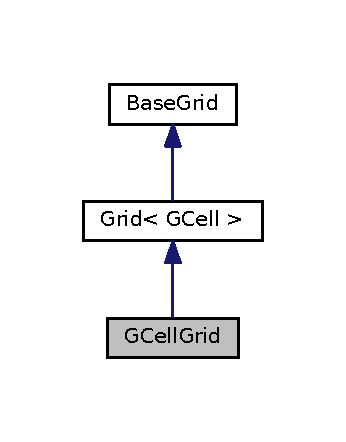
\includegraphics[width=166pt]{classKatabatic_1_1GCellGrid__inherit__graph}
\end{center}
\end{figure}
\subsection*{Public Types}
\begin{DoxyCompactItemize}
\item 
enum \mbox{\hyperlink{classKatabatic_1_1GCellGrid_a07884f5e1af410e98208fed76a2b40fe}{Density\+Mode}} \{ \newline
\mbox{\hyperlink{classKatabatic_1_1GCellGrid_a07884f5e1af410e98208fed76a2b40fead15bf3e5b63f398d76d717a088acd310}{Average\+H\+V\+Density}} =1, 
\newline
\mbox{\hyperlink{classKatabatic_1_1GCellGrid_a07884f5e1af410e98208fed76a2b40feaec0ad06385eae8d1e2dee4f3c9f9f4ed}{Average\+H\+Density}} =2, 
\newline
\mbox{\hyperlink{classKatabatic_1_1GCellGrid_a07884f5e1af410e98208fed76a2b40fead1a1d89017d10aeb63d1c05b6fb650dd}{Average\+V\+Density}} =3, 
\newline
\mbox{\hyperlink{classKatabatic_1_1GCellGrid_a07884f5e1af410e98208fed76a2b40fea8265e053af0708a508ecbce86d1a8165}{Max\+H\+V\+Density}} =4, 
\newline
\mbox{\hyperlink{classKatabatic_1_1GCellGrid_a07884f5e1af410e98208fed76a2b40fea5f0a89ca367ef98550eaa86c1e32c873}{Max\+V\+Density}} =5, 
\newline
\mbox{\hyperlink{classKatabatic_1_1GCellGrid_a07884f5e1af410e98208fed76a2b40fea2a6d29b012cc89026c3c0061f87a4f03}{Max\+H\+Density}} =6, 
\newline
\mbox{\hyperlink{classKatabatic_1_1GCellGrid_a07884f5e1af410e98208fed76a2b40fea90a2f4a4ee8558de9f99458ddeab852c}{Max\+Density}} =7
 \}
\end{DoxyCompactItemize}
\subsection*{Public Member Functions}
\begin{DoxyCompactItemize}
\item 
\textbf{ Cell} $\ast$ \mbox{\hyperlink{classKatabatic_1_1GCellGrid_a55a3a88610ef1af9931e634f77f2403b}{get\+Cell}} () const
\item 
\mbox{\hyperlink{classKatabatic_1_1KatabaticEngine}{Katabatic\+Engine}} $\ast$ \mbox{\hyperlink{classKatabatic_1_1GCellGrid_a0234fdabe7682546f1201bccd0b5cacf}{get\+Katabatic}} () const
\item 
unsigned int \mbox{\hyperlink{classKatabatic_1_1GCellGrid_af1171855a3e928cace78d1534a8d0629}{get\+Density\+Mode}} () const
\item 
size\+\_\+t \mbox{\hyperlink{classKatabatic_1_1GCellGrid_a041680c5d171d4c7cb0edba96f0c390f}{get\+H\+Edge\+Capacity}} () const
\item 
size\+\_\+t \mbox{\hyperlink{classKatabatic_1_1GCellGrid_ae8e2cf3685ccb0621f4f85c7999834e8}{get\+V\+Edge\+Capacity}} () const
\item 
\textbf{ Interval} \mbox{\hyperlink{classKatabatic_1_1GCellGrid_a8272dad8f7d916333f934f3cbde981bb}{get\+U\+Side}} (unsigned int) const
\item 
size\+\_\+t \mbox{\hyperlink{classKatabatic_1_1GCellGrid_a88208864ba2268689946a8cb7a86fcb2}{check\+Density}} () const
\item 
size\+\_\+t \mbox{\hyperlink{classKatabatic_1_1GCellGrid_a9b3455dce10eb98d0496175dd586528c}{update\+Density}} ()
\item 
void \mbox{\hyperlink{classKatabatic_1_1GCellGrid_a032d6eb23f92e3a41a020d18c6bbc02d}{update\+Contacts}} (unsigned int flags=\mbox{\hyperlink{namespaceKatabatic_a2af2ad6b6441614038caf59d04b3b217af314588109fcc5f5ee1c42e5fd4d0ed5}{Kb\+Open\+Session}})
\item 
void \mbox{\hyperlink{classKatabatic_1_1GCellGrid_a86899930041463cf80b713c3ca5b4834}{set\+Density\+Mode}} (unsigned int)
\end{DoxyCompactItemize}
\subsection*{Protected Member Functions}
\begin{DoxyCompactItemize}
\item 
void \mbox{\hyperlink{classKatabatic_1_1GCellGrid_a3715b38135ca24745f610bebd3407c10}{\+\_\+post\+Create}} ()
\item 
void \mbox{\hyperlink{classKatabatic_1_1GCellGrid_a7c13d9795eafd477994961f8a0d962d0}{\+\_\+pre\+Destroy}} ()
\end{DoxyCompactItemize}
\subsection*{Static Protected Member Functions}
\begin{DoxyCompactItemize}
\item 
static \mbox{\hyperlink{classKatabatic_1_1GCellGrid}{G\+Cell\+Grid}} $\ast$ \mbox{\hyperlink{classKatabatic_1_1GCellGrid_a19a45b2e6c6b9ca8898b2fde035d1827}{create}} (\mbox{\hyperlink{classKatabatic_1_1KatabaticEngine}{Katabatic\+Engine}} $\ast$)
\end{DoxyCompactItemize}


\subsection{Detailed Description}
\mbox{\hyperlink{classKatabatic_1_1GCell}{G\+Cell}} \mbox{\hyperlink{classKatabatic_1_1Grid}{Grid}}. 

The \mbox{\hyperlink{classKatabatic_1_1GCell}{G\+Cell}} \mbox{\hyperlink{classKatabatic_1_1Grid}{Grid}} of \mbox{\hyperlink{namespaceKatabatic}{Katabatic}}. Although the base template class \mbox{\hyperlink{classKatabatic_1_1Grid}{Grid}} support irregular grid, the \mbox{\hyperlink{classKatabatic_1_1GCellGrid}{G\+Cell\+Grid}} is regular, following the Knik global router G\+Cells. Only the topmost row and leftmost column may have different height or width to cope with the design real size.

Due to the regular nature of the grid, the horizontal \& vertical edges capacities are all identical, and initialized from the \mbox{\hyperlink{namespaceKatabatic}{Katabatic}} Configuration.

The grid is build from the Knik global routing, so obviously a Knik\+Engine must be attached to the Cell when building the \mbox{\hyperlink{classKatabatic_1_1GCellGrid}{G\+Cell\+Grid}}. An error is thrown otherwise. 

\subsection{Member Enumeration Documentation}
\mbox{\Hypertarget{classKatabatic_1_1GCellGrid_a07884f5e1af410e98208fed76a2b40fe}\label{classKatabatic_1_1GCellGrid_a07884f5e1af410e98208fed76a2b40fe}} 
\index{Katabatic\+::\+G\+Cell\+Grid@{Katabatic\+::\+G\+Cell\+Grid}!Density\+Mode@{Density\+Mode}}
\index{Density\+Mode@{Density\+Mode}!Katabatic\+::\+G\+Cell\+Grid@{Katabatic\+::\+G\+Cell\+Grid}}
\subsubsection{\texorpdfstring{Density\+Mode}{DensityMode}}
{\footnotesize\ttfamily enum \mbox{\hyperlink{classKatabatic_1_1GCellGrid_a07884f5e1af410e98208fed76a2b40fe}{Density\+Mode}}}

Various ways of computing the overall density of a \mbox{\hyperlink{classKatabatic_1_1GCell}{G\+Cell}}. \begin{DoxyEnumFields}{Enumerator}
\raisebox{\heightof{T}}[0pt][0pt]{\index{Average\+H\+V\+Density@{Average\+H\+V\+Density}!Katabatic\+::\+G\+Cell\+Grid@{Katabatic\+::\+G\+Cell\+Grid}}\index{Katabatic\+::\+G\+Cell\+Grid@{Katabatic\+::\+G\+Cell\+Grid}!Average\+H\+V\+Density@{Average\+H\+V\+Density}}}\mbox{\Hypertarget{classKatabatic_1_1GCellGrid_a07884f5e1af410e98208fed76a2b40fead15bf3e5b63f398d76d717a088acd310}\label{classKatabatic_1_1GCellGrid_a07884f5e1af410e98208fed76a2b40fead15bf3e5b63f398d76d717a088acd310}} 
Average\+H\+V\+Density&The average density all depths accounted. \\
\hline

\raisebox{\heightof{T}}[0pt][0pt]{\index{Average\+H\+Density@{Average\+H\+Density}!Katabatic\+::\+G\+Cell\+Grid@{Katabatic\+::\+G\+Cell\+Grid}}\index{Katabatic\+::\+G\+Cell\+Grid@{Katabatic\+::\+G\+Cell\+Grid}!Average\+H\+Density@{Average\+H\+Density}}}\mbox{\Hypertarget{classKatabatic_1_1GCellGrid_a07884f5e1af410e98208fed76a2b40feaec0ad06385eae8d1e2dee4f3c9f9f4ed}\label{classKatabatic_1_1GCellGrid_a07884f5e1af410e98208fed76a2b40feaec0ad06385eae8d1e2dee4f3c9f9f4ed}} 
Average\+H\+Density&The average density of horizontal layers. \\
\hline

\raisebox{\heightof{T}}[0pt][0pt]{\index{Average\+V\+Density@{Average\+V\+Density}!Katabatic\+::\+G\+Cell\+Grid@{Katabatic\+::\+G\+Cell\+Grid}}\index{Katabatic\+::\+G\+Cell\+Grid@{Katabatic\+::\+G\+Cell\+Grid}!Average\+V\+Density@{Average\+V\+Density}}}\mbox{\Hypertarget{classKatabatic_1_1GCellGrid_a07884f5e1af410e98208fed76a2b40fead1a1d89017d10aeb63d1c05b6fb650dd}\label{classKatabatic_1_1GCellGrid_a07884f5e1af410e98208fed76a2b40fead1a1d89017d10aeb63d1c05b6fb650dd}} 
Average\+V\+Density&The average density of horizontal layers. \\
\hline

\raisebox{\heightof{T}}[0pt][0pt]{\index{Max\+H\+V\+Density@{Max\+H\+V\+Density}!Katabatic\+::\+G\+Cell\+Grid@{Katabatic\+::\+G\+Cell\+Grid}}\index{Katabatic\+::\+G\+Cell\+Grid@{Katabatic\+::\+G\+Cell\+Grid}!Max\+H\+V\+Density@{Max\+H\+V\+Density}}}\mbox{\Hypertarget{classKatabatic_1_1GCellGrid_a07884f5e1af410e98208fed76a2b40fea8265e053af0708a508ecbce86d1a8165}\label{classKatabatic_1_1GCellGrid_a07884f5e1af410e98208fed76a2b40fea8265e053af0708a508ecbce86d1a8165}} 
Max\+H\+V\+Density&The maximum of the average horizontal \& vertical densities taken as a whole. \\
\hline

\raisebox{\heightof{T}}[0pt][0pt]{\index{Max\+V\+Density@{Max\+V\+Density}!Katabatic\+::\+G\+Cell\+Grid@{Katabatic\+::\+G\+Cell\+Grid}}\index{Katabatic\+::\+G\+Cell\+Grid@{Katabatic\+::\+G\+Cell\+Grid}!Max\+V\+Density@{Max\+V\+Density}}}\mbox{\Hypertarget{classKatabatic_1_1GCellGrid_a07884f5e1af410e98208fed76a2b40fea5f0a89ca367ef98550eaa86c1e32c873}\label{classKatabatic_1_1GCellGrid_a07884f5e1af410e98208fed76a2b40fea5f0a89ca367ef98550eaa86c1e32c873}} 
Max\+V\+Density&The maximum of the average vertical densities taken depth by depth. \\
\hline

\raisebox{\heightof{T}}[0pt][0pt]{\index{Max\+H\+Density@{Max\+H\+Density}!Katabatic\+::\+G\+Cell\+Grid@{Katabatic\+::\+G\+Cell\+Grid}}\index{Katabatic\+::\+G\+Cell\+Grid@{Katabatic\+::\+G\+Cell\+Grid}!Max\+H\+Density@{Max\+H\+Density}}}\mbox{\Hypertarget{classKatabatic_1_1GCellGrid_a07884f5e1af410e98208fed76a2b40fea2a6d29b012cc89026c3c0061f87a4f03}\label{classKatabatic_1_1GCellGrid_a07884f5e1af410e98208fed76a2b40fea2a6d29b012cc89026c3c0061f87a4f03}} 
Max\+H\+Density&The maximum of the average horizontal densities taken depth by depth. \\
\hline

\raisebox{\heightof{T}}[0pt][0pt]{\index{Max\+Density@{Max\+Density}!Katabatic\+::\+G\+Cell\+Grid@{Katabatic\+::\+G\+Cell\+Grid}}\index{Katabatic\+::\+G\+Cell\+Grid@{Katabatic\+::\+G\+Cell\+Grid}!Max\+Density@{Max\+Density}}}\mbox{\Hypertarget{classKatabatic_1_1GCellGrid_a07884f5e1af410e98208fed76a2b40fea90a2f4a4ee8558de9f99458ddeab852c}\label{classKatabatic_1_1GCellGrid_a07884f5e1af410e98208fed76a2b40fea90a2f4a4ee8558de9f99458ddeab852c}} 
Max\+Density&The maximum of the average horizontal \& vertical densities taken depth by depth. \\
\hline

\end{DoxyEnumFields}


\subsection{Member Function Documentation}
\mbox{\Hypertarget{classKatabatic_1_1GCellGrid_a55a3a88610ef1af9931e634f77f2403b}\label{classKatabatic_1_1GCellGrid_a55a3a88610ef1af9931e634f77f2403b}} 
\index{Katabatic\+::\+G\+Cell\+Grid@{Katabatic\+::\+G\+Cell\+Grid}!get\+Cell@{get\+Cell}}
\index{get\+Cell@{get\+Cell}!Katabatic\+::\+G\+Cell\+Grid@{Katabatic\+::\+G\+Cell\+Grid}}
\subsubsection{\texorpdfstring{get\+Cell()}{getCell()}}
{\footnotesize\ttfamily \textbf{ Cell} $\ast$ get\+Cell (\begin{DoxyParamCaption}{ }\end{DoxyParamCaption}) const}

{\bfseries Returns\+:} The associated Cell. 

Referenced by G\+Cell\+Grid\+::\+\_\+post\+Create().

\mbox{\Hypertarget{classKatabatic_1_1GCellGrid_a0234fdabe7682546f1201bccd0b5cacf}\label{classKatabatic_1_1GCellGrid_a0234fdabe7682546f1201bccd0b5cacf}} 
\index{Katabatic\+::\+G\+Cell\+Grid@{Katabatic\+::\+G\+Cell\+Grid}!get\+Katabatic@{get\+Katabatic}}
\index{get\+Katabatic@{get\+Katabatic}!Katabatic\+::\+G\+Cell\+Grid@{Katabatic\+::\+G\+Cell\+Grid}}
\subsubsection{\texorpdfstring{get\+Katabatic()}{getKatabatic()}}
{\footnotesize\ttfamily \mbox{\hyperlink{classKatabatic_1_1KatabaticEngine}{Katabatic\+Engine}} $\ast$ get\+Katabatic (\begin{DoxyParamCaption}{ }\end{DoxyParamCaption}) const\hspace{0.3cm}{\ttfamily [inline]}}

{\bfseries Returns\+:} The associated \mbox{\hyperlink{classKatabatic_1_1KatabaticEngine}{Katabatic\+Engine}}. \mbox{\Hypertarget{classKatabatic_1_1GCellGrid_af1171855a3e928cace78d1534a8d0629}\label{classKatabatic_1_1GCellGrid_af1171855a3e928cace78d1534a8d0629}} 
\index{Katabatic\+::\+G\+Cell\+Grid@{Katabatic\+::\+G\+Cell\+Grid}!get\+Density\+Mode@{get\+Density\+Mode}}
\index{get\+Density\+Mode@{get\+Density\+Mode}!Katabatic\+::\+G\+Cell\+Grid@{Katabatic\+::\+G\+Cell\+Grid}}
\subsubsection{\texorpdfstring{get\+Density\+Mode()}{getDensityMode()}}
{\footnotesize\ttfamily unsigned int get\+Density\+Mode (\begin{DoxyParamCaption}{ }\end{DoxyParamCaption}) const\hspace{0.3cm}{\ttfamily [inline]}}

{\bfseries Returns\+:} The computation mode of the \mbox{\hyperlink{classKatabatic_1_1GCell}{G\+Cell}} densities. 

Referenced by G\+Cell\+::get\+Density().

\mbox{\Hypertarget{classKatabatic_1_1GCellGrid_a041680c5d171d4c7cb0edba96f0c390f}\label{classKatabatic_1_1GCellGrid_a041680c5d171d4c7cb0edba96f0c390f}} 
\index{Katabatic\+::\+G\+Cell\+Grid@{Katabatic\+::\+G\+Cell\+Grid}!get\+H\+Edge\+Capacity@{get\+H\+Edge\+Capacity}}
\index{get\+H\+Edge\+Capacity@{get\+H\+Edge\+Capacity}!Katabatic\+::\+G\+Cell\+Grid@{Katabatic\+::\+G\+Cell\+Grid}}
\subsubsection{\texorpdfstring{get\+H\+Edge\+Capacity()}{getHEdgeCapacity()}}
{\footnotesize\ttfamily size\+\_\+t get\+H\+Edge\+Capacity (\begin{DoxyParamCaption}{ }\end{DoxyParamCaption}) const\hspace{0.3cm}{\ttfamily [inline]}}

{\bfseries Returns\+:} The horizontal edge capacity. As the matrix is regular it is identical for all horizontal edges. 

Referenced by G\+Cell\+::check\+Edge\+Saturation().

\mbox{\Hypertarget{classKatabatic_1_1GCellGrid_ae8e2cf3685ccb0621f4f85c7999834e8}\label{classKatabatic_1_1GCellGrid_ae8e2cf3685ccb0621f4f85c7999834e8}} 
\index{Katabatic\+::\+G\+Cell\+Grid@{Katabatic\+::\+G\+Cell\+Grid}!get\+V\+Edge\+Capacity@{get\+V\+Edge\+Capacity}}
\index{get\+V\+Edge\+Capacity@{get\+V\+Edge\+Capacity}!Katabatic\+::\+G\+Cell\+Grid@{Katabatic\+::\+G\+Cell\+Grid}}
\subsubsection{\texorpdfstring{get\+V\+Edge\+Capacity()}{getVEdgeCapacity()}}
{\footnotesize\ttfamily size\+\_\+t get\+V\+Edge\+Capacity (\begin{DoxyParamCaption}{ }\end{DoxyParamCaption}) const\hspace{0.3cm}{\ttfamily [inline]}}

{\bfseries Returns\+:} The vertical edge capacity. As the matrix is regular it is identical for all vertical edges. 

Referenced by G\+Cell\+::check\+Edge\+Saturation().

\mbox{\Hypertarget{classKatabatic_1_1GCellGrid_a8272dad8f7d916333f934f3cbde981bb}\label{classKatabatic_1_1GCellGrid_a8272dad8f7d916333f934f3cbde981bb}} 
\index{Katabatic\+::\+G\+Cell\+Grid@{Katabatic\+::\+G\+Cell\+Grid}!get\+U\+Side@{get\+U\+Side}}
\index{get\+U\+Side@{get\+U\+Side}!Katabatic\+::\+G\+Cell\+Grid@{Katabatic\+::\+G\+Cell\+Grid}}
\subsubsection{\texorpdfstring{get\+U\+Side()}{getUSide()}}
{\footnotesize\ttfamily \textbf{ Interval} get\+U\+Side (\begin{DoxyParamCaption}\item[{unsigned int}]{direction }\end{DoxyParamCaption}) const}

{\bfseries Returns\+:} The side of the whole grid in {\ttfamily direction}. 

References Box\+::get\+X\+Max(), Box\+::get\+X\+Min(), Box\+::get\+Y\+Max(), Box\+::get\+Y\+Min(), Katabatic\+::\+Kb\+Horizontal, and Katabatic\+::\+Kb\+Vertical.

\mbox{\Hypertarget{classKatabatic_1_1GCellGrid_a88208864ba2268689946a8cb7a86fcb2}\label{classKatabatic_1_1GCellGrid_a88208864ba2268689946a8cb7a86fcb2}} 
\index{Katabatic\+::\+G\+Cell\+Grid@{Katabatic\+::\+G\+Cell\+Grid}!check\+Density@{check\+Density}}
\index{check\+Density@{check\+Density}!Katabatic\+::\+G\+Cell\+Grid@{Katabatic\+::\+G\+Cell\+Grid}}
\subsubsection{\texorpdfstring{check\+Density()}{checkDensity()}}
{\footnotesize\ttfamily size\+\_\+t check\+Density (\begin{DoxyParamCaption}{ }\end{DoxyParamCaption}) const}

{\bfseries Returns\+:} The number of \mbox{\hyperlink{classKatabatic_1_1GCell}{G\+Cell}} saturateds.

Check all G\+Cells for saturations. 

References Grid$<$ G\+Cell $>$\+::get\+G\+Cells().

\mbox{\Hypertarget{classKatabatic_1_1GCellGrid_a9b3455dce10eb98d0496175dd586528c}\label{classKatabatic_1_1GCellGrid_a9b3455dce10eb98d0496175dd586528c}} 
\index{Katabatic\+::\+G\+Cell\+Grid@{Katabatic\+::\+G\+Cell\+Grid}!update\+Density@{update\+Density}}
\index{update\+Density@{update\+Density}!Katabatic\+::\+G\+Cell\+Grid@{Katabatic\+::\+G\+Cell\+Grid}}
\subsubsection{\texorpdfstring{update\+Density()}{updateDensity()}}
{\footnotesize\ttfamily size\+\_\+t update\+Density (\begin{DoxyParamCaption}{ }\end{DoxyParamCaption})}

{\bfseries Returns\+:} The number of \mbox{\hyperlink{classKatabatic_1_1GCell}{G\+Cell}} saturateds.

Force a density update on all the G\+Cells. 

References Grid$<$ G\+Cell $>$\+::get\+G\+Cells().

\mbox{\Hypertarget{classKatabatic_1_1GCellGrid_a032d6eb23f92e3a41a020d18c6bbc02d}\label{classKatabatic_1_1GCellGrid_a032d6eb23f92e3a41a020d18c6bbc02d}} 
\index{Katabatic\+::\+G\+Cell\+Grid@{Katabatic\+::\+G\+Cell\+Grid}!update\+Contacts@{update\+Contacts}}
\index{update\+Contacts@{update\+Contacts}!Katabatic\+::\+G\+Cell\+Grid@{Katabatic\+::\+G\+Cell\+Grid}}
\subsubsection{\texorpdfstring{update\+Contacts()}{updateContacts()}}
{\footnotesize\ttfamily void update\+Contacts (\begin{DoxyParamCaption}\item[{unsigned int}]{flags = {\ttfamily \mbox{\hyperlink{namespaceKatabatic_a2af2ad6b6441614038caf59d04b3b217af314588109fcc5f5ee1c42e5fd4d0ed5}{Kb\+Open\+Session}}} }\end{DoxyParamCaption})}

Force an update on all \mbox{\hyperlink{classKatabatic_1_1AutoContact}{Auto\+Contact}} on all the G\+Cells. if {\ttfamily open\+Session} is {\bfseries true}, enclose the update in a \mbox{\hyperlink{classKatabatic_1_1Session}{Session}}. 

References Session\+::close(), Grid$<$ G\+Cell $>$\+::get\+G\+Cells(), Katabatic\+::\+Kb\+Open\+Session, and Session\+::open().



Referenced by Katabatic\+Engine\+::refresh().

\mbox{\Hypertarget{classKatabatic_1_1GCellGrid_a86899930041463cf80b713c3ca5b4834}\label{classKatabatic_1_1GCellGrid_a86899930041463cf80b713c3ca5b4834}} 
\index{Katabatic\+::\+G\+Cell\+Grid@{Katabatic\+::\+G\+Cell\+Grid}!set\+Density\+Mode@{set\+Density\+Mode}}
\index{set\+Density\+Mode@{set\+Density\+Mode}!Katabatic\+::\+G\+Cell\+Grid@{Katabatic\+::\+G\+Cell\+Grid}}
\subsubsection{\texorpdfstring{set\+Density\+Mode()}{setDensityMode()}}
{\footnotesize\ttfamily void set\+Density\+Mode (\begin{DoxyParamCaption}\item[{unsigned int}]{mode }\end{DoxyParamCaption})\hspace{0.3cm}{\ttfamily [inline]}}

Sets the density computation mode. \mbox{\Hypertarget{classKatabatic_1_1GCellGrid_a3715b38135ca24745f610bebd3407c10}\label{classKatabatic_1_1GCellGrid_a3715b38135ca24745f610bebd3407c10}} 
\index{Katabatic\+::\+G\+Cell\+Grid@{Katabatic\+::\+G\+Cell\+Grid}!\+\_\+post\+Create@{\+\_\+post\+Create}}
\index{\+\_\+post\+Create@{\+\_\+post\+Create}!Katabatic\+::\+G\+Cell\+Grid@{Katabatic\+::\+G\+Cell\+Grid}}
\subsubsection{\texorpdfstring{\+\_\+post\+Create()}{\_postCreate()}}
{\footnotesize\ttfamily void \+\_\+post\+Create (\begin{DoxyParamCaption}{ }\end{DoxyParamCaption})\hspace{0.3cm}{\ttfamily [protected]}, {\ttfamily [virtual]}}

Perform the \mbox{\hyperlink{classKatabatic_1_1GCell}{G\+Cell}} \& \mbox{\hyperlink{classKatabatic_1_1GCell}{G\+Cell}} vector allocation.
\begin{DoxyItemize}
\item Read the horizontal and vertical cut lines from Knik and translate them into \mbox{\hyperlink{classKatabatic_1_1BaseGrid_1_1Axis}{Base\+Grid\+::\+Axis}}.
\item From the \mbox{\hyperlink{classKatabatic_1_1BaseGrid_1_1Axis}{Base\+Grid\+::\+Axis}}, deduces the exact positions of the G\+Cells and allocate them.
\item The \mbox{\hyperlink{classKatabatic_1_1GCell}{G\+Cell}} allocation is done in a \char`\"{}row by row\char`\"{} fashion consistent with \mbox{\hyperlink{classKatabatic_1_1BaseGrid}{Base\+Grid}} implicit assumptions. 
\end{DoxyItemize}

Reimplemented from \mbox{\hyperlink{classKatabatic_1_1BaseGrid}{Base\+Grid}}.



References Base\+Grid\+::\+Axis\+::add\+Graduation(), G\+Cell\+Grid\+::get\+Cell(), Base\+Grid\+::get\+Columns(), Base\+Grid\+::get\+Rows(), Base\+Grid\+::\+Axis\+::get\+Size(), and Base\+Grid\+::\+Axis\+::sort().

\mbox{\Hypertarget{classKatabatic_1_1GCellGrid_a7c13d9795eafd477994961f8a0d962d0}\label{classKatabatic_1_1GCellGrid_a7c13d9795eafd477994961f8a0d962d0}} 
\index{Katabatic\+::\+G\+Cell\+Grid@{Katabatic\+::\+G\+Cell\+Grid}!\+\_\+pre\+Destroy@{\+\_\+pre\+Destroy}}
\index{\+\_\+pre\+Destroy@{\+\_\+pre\+Destroy}!Katabatic\+::\+G\+Cell\+Grid@{Katabatic\+::\+G\+Cell\+Grid}}
\subsubsection{\texorpdfstring{\+\_\+pre\+Destroy()}{\_preDestroy()}}
{\footnotesize\ttfamily void \+\_\+pre\+Destroy (\begin{DoxyParamCaption}{ }\end{DoxyParamCaption})\hspace{0.3cm}{\ttfamily [protected]}, {\ttfamily [virtual]}}

The G\+Cells are deleted at this point. 

Reimplemented from \mbox{\hyperlink{classKatabatic_1_1BaseGrid}{Base\+Grid}}.

\mbox{\Hypertarget{classKatabatic_1_1GCellGrid_a19a45b2e6c6b9ca8898b2fde035d1827}\label{classKatabatic_1_1GCellGrid_a19a45b2e6c6b9ca8898b2fde035d1827}} 
\index{Katabatic\+::\+G\+Cell\+Grid@{Katabatic\+::\+G\+Cell\+Grid}!create@{create}}
\index{create@{create}!Katabatic\+::\+G\+Cell\+Grid@{Katabatic\+::\+G\+Cell\+Grid}}
\subsubsection{\texorpdfstring{create()}{create()}}
{\footnotesize\ttfamily \mbox{\hyperlink{classKatabatic_1_1GCellGrid}{G\+Cell\+Grid}} $\ast$ create (\begin{DoxyParamCaption}\item[{\mbox{\hyperlink{classKatabatic_1_1KatabaticEngine}{Katabatic\+Engine}} $\ast$}]{ktbt }\end{DoxyParamCaption})\hspace{0.3cm}{\ttfamily [static]}, {\ttfamily [protected]}}

A\+P\+I-\/space contructor. 

References grid().



Referenced by Katabatic\+Engine\+::create\+Detailed\+Grid().



The documentation for this class was generated from the following files\+:\begin{DoxyCompactItemize}
\item 
G\+Cell\+Grid.\+h\item 
G\+Cell\+Grid.\+cpp\item 
G\+Cell\+Grid.\+dox\end{DoxyCompactItemize}

\hypertarget{classanonymous__namespace_02LoadGrByNet_8cpp_03_1_1GCellTopology}{}\section{G\+Cell\+Topology Class Reference}
\label{classanonymous__namespace_02LoadGrByNet_8cpp_03_1_1GCellTopology}\index{G\+Cell\+Topology@{G\+Cell\+Topology}}


Build the wiring for a Net inside a G\+Cell ({\bfseries internal}).  


\subsection*{Static Public Member Functions}
\begin{DoxyCompactItemize}
\item 
static void \mbox{\hyperlink{group__LoadGlobalRouting_gae9cae408ea16a3f7c77c3d75f0242f19}{do\+Rp\+\_\+\+Auto\+Contacts}} (\mbox{\hyperlink{classKatabatic_1_1GCell}{G\+Cell}} $\ast$, \textbf{ Component} $\ast$, \mbox{\hyperlink{classKatabatic_1_1AutoContact}{Auto\+Contact}} $\ast$\&source, \mbox{\hyperlink{classKatabatic_1_1AutoContact}{Auto\+Contact}} $\ast$\&target, unsigned int flags)
\item 
static \mbox{\hyperlink{classKatabatic_1_1AutoContact}{Auto\+Contact}} $\ast$ \mbox{\hyperlink{group__LoadGlobalRouting_gada6d3c694b8d741b6504b7c3da166357}{do\+Rp\+\_\+\+Access}} (\mbox{\hyperlink{classKatabatic_1_1GCell}{G\+Cell}} $\ast$, \textbf{ Component} $\ast$, unsigned int flags)
\item 
static \mbox{\hyperlink{classKatabatic_1_1AutoContact}{Auto\+Contact}} $\ast$ \mbox{\hyperlink{group__LoadGlobalRouting_ga60edeea78b56db072fc26a58a7afbcd4}{do\+Rp\+\_\+\+Access\+Pad}} (\textbf{ Routing\+Pad} $\ast$, unsigned int flags)
\item 
static void \mbox{\hyperlink{group__LoadGlobalRouting_ga3291d84592215974fe4052c00304bdb1}{do\+Rp\+\_\+\+Stair\+CaseH}} (\mbox{\hyperlink{classKatabatic_1_1GCell}{G\+Cell}} $\ast$, \textbf{ Component} $\ast$rp1, \textbf{ Component} $\ast$rp2)
\item 
static void \mbox{\hyperlink{group__LoadGlobalRouting_ga6361fb0e90f35cd59063a1ee971ef2a9}{do\+Rp\+\_\+\+Stair\+CaseV}} (\mbox{\hyperlink{classKatabatic_1_1GCell}{G\+Cell}} $\ast$, \textbf{ Component} $\ast$rp1, \textbf{ Component} $\ast$rp2)
\end{DoxyCompactItemize}
\subsection*{Private Member Functions}
\begin{DoxyCompactItemize}
\item 
void \mbox{\hyperlink{group__LoadGlobalRouting_gaaa6d4ccd2eadfb6bc3e2cc98cfaf2cca}{\+\_\+do\+\_\+xG}} ()
\item 
void \mbox{\hyperlink{group__LoadGlobalRouting_gabe00ab10a0dab8a3d2de0709e61e4e7d}{\+\_\+do\+\_\+x\+G\+\_\+1\+Pad}} ()
\item 
void \mbox{\hyperlink{group__LoadGlobalRouting_gad24a03e87e269f16dcc28d8c2d9f1cfb}{\+\_\+do\+\_\+1\+G\+\_\+1\+M1}} ()
\item 
void \mbox{\hyperlink{group__LoadGlobalRouting_ga97942453a1bc5b01106aa380271fd7fc}{\+\_\+do\+\_\+1\+G\+\_\+x\+M1}} ()
\item 
void \mbox{\hyperlink{group__LoadGlobalRouting_gaf9b009520f54099668ac9d12f2c85257}{\+\_\+do\+\_\+x\+G\+\_\+x\+M1\+\_\+x\+M3}} ()
\item 
void \mbox{\hyperlink{group__LoadGlobalRouting_gae60ed4e27ad89a1e2ff2cd6415ef33f1}{\+\_\+do\+\_\+x\+G\+\_\+1\+M1\+\_\+1\+M2}} ()
\item 
void \mbox{\hyperlink{group__LoadGlobalRouting_ga532d1c6b530e0375078ea2d6ea3c6024}{\+\_\+do\+\_\+x\+G\+\_\+x\+M2}} ()
\item 
void \mbox{\hyperlink{group__LoadGlobalRouting_ga2519ef984b3d19f123827a9b12651672}{\+\_\+do\+\_\+1\+G\+\_\+1\+M3}} ()
\item 
void \mbox{\hyperlink{group__LoadGlobalRouting_ga007efc725aae31782204a44949765cb4}{\+\_\+do\+\_\+x\+G\+\_\+x\+M3}} ()
\end{DoxyCompactItemize}


\subsection{Detailed Description}
Build the wiring for a Net inside a G\+Cell ({\bfseries internal}). 

As this class is called to initially construct the \mbox{\hyperlink{namespaceKatabatic}{Katabatic}} wiring, it must build a {\bfseries connex} wiring. That is without gaps in layer depth, because the topology restauration mechanism (\mbox{\hyperlink{classKatabatic_1_1AutoContact_a690764ddc997fe9766a79c4b8e0c3e2f}{Auto\+Contact\+::update\+Topology()}}) of the Auto\+Contact cannot work until all Auto\+Segments are revalidated at least once. The topology restauration work by creating doglegs which in turn, call the canonization, which needs all the caches to be up to date. 

The documentation for this class was generated from the following file\+:\begin{DoxyCompactItemize}
\item 
Load\+Gr\+By\+Net.\+cpp\end{DoxyCompactItemize}

\hypertarget{classKatabatic_1_1Grid}{}\section{Grid$<$ G\+CellT $>$ Class Template Reference}
\label{classKatabatic_1_1Grid}\index{Grid$<$ G\+Cell\+T $>$@{Grid$<$ G\+Cell\+T $>$}}


Template Class for Regular \mbox{\hyperlink{classKatabatic_1_1Grid}{Grid}}.  




Inheritance diagram for Grid$<$ G\+CellT $>$\+:\nopagebreak
\begin{figure}[H]
\begin{center}
\leavevmode
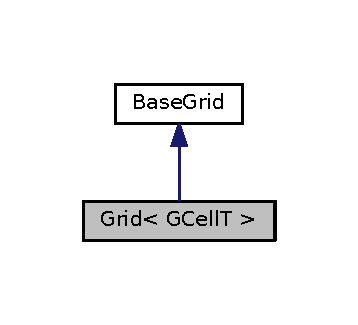
\includegraphics[width=172pt]{classKatabatic_1_1Grid__inherit__graph}
\end{center}
\end{figure}
\subsection*{Public Member Functions}
\begin{DoxyCompactItemize}
\item 
G\+CellT $\ast$ \mbox{\hyperlink{classKatabatic_1_1Grid_a98650c11b4aa0c6107c4d890dff61587}{get\+G\+Cell}} (unsigned int index) const
\item 
G\+CellT $\ast$ \mbox{\hyperlink{classKatabatic_1_1Grid_a0ee3cd2fb8c66458b0d00e39826921da}{get\+G\+Cell}} (const \textbf{ Point} p) const
\item 
G\+CellT $\ast$ \mbox{\hyperlink{classKatabatic_1_1Grid_a1beb5c490b2e651eab49178297b6cda2}{get\+G\+Cell}} (const \textbf{ Point} p1, const \textbf{ Point} p2) const
\item 
G\+CellT $\ast$ \mbox{\hyperlink{classKatabatic_1_1Grid_ae5041816e75468b69bb0bbf24a4e8eca}{get\+G\+Cell\+Left}} (const G\+CellT $\ast$gcell) const
\item 
G\+CellT $\ast$ \mbox{\hyperlink{classKatabatic_1_1Grid_a0e9bba0feb437dca932d59703298358e}{get\+G\+Cell\+Right}} (const G\+CellT $\ast$gcell) const
\item 
G\+CellT $\ast$ \mbox{\hyperlink{classKatabatic_1_1Grid_a3a22f2bce9124765eb937b78c90059a0}{get\+G\+Cell\+Up}} (const G\+CellT $\ast$gcell) const
\item 
G\+CellT $\ast$ \mbox{\hyperlink{classKatabatic_1_1Grid_a4288eb8b1357d9800341b82df6b23944}{get\+G\+Cell\+Down}} (const G\+CellT $\ast$gcell) const
\item 
\textbf{ Generic\+Collection}$<$ G\+CellT $\ast$ $>$ \mbox{\hyperlink{classKatabatic_1_1Grid_a24b4ab5b46b56ee744cf4c368a114d95}{get\+G\+Cells}} ()
\item 
\textbf{ Generic\+Collection}$<$ G\+CellT $\ast$ $>$ \mbox{\hyperlink{classKatabatic_1_1Grid_aa8d0393323104d48c089a8429b254689}{get\+G\+Cells\+Column}} (unsigned int column, unsigned int row\+Start, unsigned int row\+Stop)
\item 
\textbf{ Generic\+Collection}$<$ G\+CellT $\ast$ $>$ \mbox{\hyperlink{classKatabatic_1_1Grid_a35e2075302cdb696945f05c5bcc817a0}{get\+G\+Cells\+Row}} (unsigned int row, unsigned int column\+Start, unsigned int column\+Stop)
\end{DoxyCompactItemize}
\subsection*{Protected Member Functions}
\begin{DoxyCompactItemize}
\item 
\mbox{\hyperlink{classKatabatic_1_1Grid_a1b772cc784f7110caca47acb76dcec62}{Grid}} (const \textbf{ Box} \&)
\end{DoxyCompactItemize}


\subsection{Detailed Description}
\subsubsection*{template$<$typename G\+CellT$>$\newline
class Katabatic\+::\+Grid$<$ G\+Cell\+T $>$}

Template Class for Regular \mbox{\hyperlink{classKatabatic_1_1Grid}{Grid}}. 

Contains all general purpose methods depending on the \mbox{\hyperlink{classKatabatic_1_1GCell}{G\+Cell}} type and geometrical computations. The internal storage is still not implemented in this class. 

\subsection{Constructor \& Destructor Documentation}
\mbox{\Hypertarget{classKatabatic_1_1Grid_a1b772cc784f7110caca47acb76dcec62}\label{classKatabatic_1_1Grid_a1b772cc784f7110caca47acb76dcec62}} 
\index{Katabatic\+::\+Grid@{Katabatic\+::\+Grid}!Grid@{Grid}}
\index{Grid@{Grid}!Katabatic\+::\+Grid@{Katabatic\+::\+Grid}}
\subsubsection{\texorpdfstring{Grid()}{Grid()}}
{\footnotesize\ttfamily \mbox{\hyperlink{classKatabatic_1_1Grid}{Grid}} (\begin{DoxyParamCaption}\item[{const \textbf{ Box} \&}]{bb }\end{DoxyParamCaption})\hspace{0.3cm}{\ttfamily [inline]}, {\ttfamily [protected]}}

\mbox{\hyperlink{classKatabatic_1_1Grid}{Grid}} constructor. 

\subsection{Member Function Documentation}
\mbox{\Hypertarget{classKatabatic_1_1Grid_a98650c11b4aa0c6107c4d890dff61587}\label{classKatabatic_1_1Grid_a98650c11b4aa0c6107c4d890dff61587}} 
\index{Katabatic\+::\+Grid@{Katabatic\+::\+Grid}!get\+G\+Cell@{get\+G\+Cell}}
\index{get\+G\+Cell@{get\+G\+Cell}!Katabatic\+::\+Grid@{Katabatic\+::\+Grid}}
\subsubsection{\texorpdfstring{get\+G\+Cell()}{getGCell()}\hspace{0.1cm}{\footnotesize\ttfamily [1/3]}}
{\footnotesize\ttfamily C\+GellT $\ast$ get\+G\+Cell (\begin{DoxyParamCaption}\item[{unsigned int}]{index }\end{DoxyParamCaption}) const\hspace{0.3cm}{\ttfamily [inline]}}

{\bfseries Returns\+:} The grid object at linear index {\ttfamily index} in the vector. If {\ttfamily index} is out of bounds, return {\ttfamily N\+U\+LL}. 

Referenced by G\+Cell\+Topology\+::do\+Rp\+\_\+\+Access\+Pad(), G\+Cell\+Topology\+::do\+Rp\+\_\+\+Auto\+Contacts(), and anonymous\+\_\+namespace\{\+Load\+Gr\+By\+Net.\+cpp\}\+::single\+G\+Cell().

\mbox{\Hypertarget{classKatabatic_1_1Grid_a0ee3cd2fb8c66458b0d00e39826921da}\label{classKatabatic_1_1Grid_a0ee3cd2fb8c66458b0d00e39826921da}} 
\index{Katabatic\+::\+Grid@{Katabatic\+::\+Grid}!get\+G\+Cell@{get\+G\+Cell}}
\index{get\+G\+Cell@{get\+G\+Cell}!Katabatic\+::\+Grid@{Katabatic\+::\+Grid}}
\subsubsection{\texorpdfstring{get\+G\+Cell()}{getGCell()}\hspace{0.1cm}{\footnotesize\ttfamily [2/3]}}
{\footnotesize\ttfamily C\+GellT $\ast$ get\+G\+Cell (\begin{DoxyParamCaption}\item[{const \textbf{ Point}}]{p }\end{DoxyParamCaption}) const\hspace{0.3cm}{\ttfamily [inline]}}

{\bfseries Returns\+:} The grid object which is under position {\ttfamily p}. \mbox{\Hypertarget{classKatabatic_1_1Grid_a1beb5c490b2e651eab49178297b6cda2}\label{classKatabatic_1_1Grid_a1beb5c490b2e651eab49178297b6cda2}} 
\index{Katabatic\+::\+Grid@{Katabatic\+::\+Grid}!get\+G\+Cell@{get\+G\+Cell}}
\index{get\+G\+Cell@{get\+G\+Cell}!Katabatic\+::\+Grid@{Katabatic\+::\+Grid}}
\subsubsection{\texorpdfstring{get\+G\+Cell()}{getGCell()}\hspace{0.1cm}{\footnotesize\ttfamily [3/3]}}
{\footnotesize\ttfamily C\+GellT $\ast$ get\+G\+Cell (\begin{DoxyParamCaption}\item[{const \textbf{ Point}}]{p1,  }\item[{const \textbf{ Point}}]{p2 }\end{DoxyParamCaption}) const\hspace{0.3cm}{\ttfamily [inline]}}

{\bfseries Returns\+:} The grid object which is under position {\ttfamily p1} and {\ttfamily p2}. Not very clear though. \mbox{\Hypertarget{classKatabatic_1_1Grid_ae5041816e75468b69bb0bbf24a4e8eca}\label{classKatabatic_1_1Grid_ae5041816e75468b69bb0bbf24a4e8eca}} 
\index{Katabatic\+::\+Grid@{Katabatic\+::\+Grid}!get\+G\+Cell\+Left@{get\+G\+Cell\+Left}}
\index{get\+G\+Cell\+Left@{get\+G\+Cell\+Left}!Katabatic\+::\+Grid@{Katabatic\+::\+Grid}}
\subsubsection{\texorpdfstring{get\+G\+Cell\+Left()}{getGCellLeft()}}
{\footnotesize\ttfamily C\+GellT $\ast$ get\+G\+Cell\+Left (\begin{DoxyParamCaption}\item[{const G\+CellT $\ast$}]{gcell }\end{DoxyParamCaption}) const\hspace{0.3cm}{\ttfamily [inline]}}

{\bfseries Returns\+:} The left neighbor of {\ttfamily gcell}, {\ttfamily N\+U\+LL} if it is the leftmost one. 

Referenced by G\+Cell\+::get\+Left().

\mbox{\Hypertarget{classKatabatic_1_1Grid_a0e9bba0feb437dca932d59703298358e}\label{classKatabatic_1_1Grid_a0e9bba0feb437dca932d59703298358e}} 
\index{Katabatic\+::\+Grid@{Katabatic\+::\+Grid}!get\+G\+Cell\+Right@{get\+G\+Cell\+Right}}
\index{get\+G\+Cell\+Right@{get\+G\+Cell\+Right}!Katabatic\+::\+Grid@{Katabatic\+::\+Grid}}
\subsubsection{\texorpdfstring{get\+G\+Cell\+Right()}{getGCellRight()}}
{\footnotesize\ttfamily C\+GellT $\ast$ get\+G\+Cell\+Right (\begin{DoxyParamCaption}\item[{const G\+CellT $\ast$}]{gcell }\end{DoxyParamCaption}) const\hspace{0.3cm}{\ttfamily [inline]}}

{\bfseries Returns\+:} The rigth neighbor of {\ttfamily gcell}, {\ttfamily N\+U\+LL} if it is the rightmost one. 

Referenced by G\+Cell\+::get\+Right().

\mbox{\Hypertarget{classKatabatic_1_1Grid_a3a22f2bce9124765eb937b78c90059a0}\label{classKatabatic_1_1Grid_a3a22f2bce9124765eb937b78c90059a0}} 
\index{Katabatic\+::\+Grid@{Katabatic\+::\+Grid}!get\+G\+Cell\+Up@{get\+G\+Cell\+Up}}
\index{get\+G\+Cell\+Up@{get\+G\+Cell\+Up}!Katabatic\+::\+Grid@{Katabatic\+::\+Grid}}
\subsubsection{\texorpdfstring{get\+G\+Cell\+Up()}{getGCellUp()}}
{\footnotesize\ttfamily C\+GellT $\ast$ get\+G\+Cell\+Up (\begin{DoxyParamCaption}\item[{const G\+CellT $\ast$}]{gcell }\end{DoxyParamCaption}) const\hspace{0.3cm}{\ttfamily [inline]}}

{\bfseries Returns\+:} The upper neighbor of {\ttfamily gcell}, {\ttfamily N\+U\+LL} if it is the uppermost one. 

Referenced by G\+Cell\+::get\+Up().

\mbox{\Hypertarget{classKatabatic_1_1Grid_a4288eb8b1357d9800341b82df6b23944}\label{classKatabatic_1_1Grid_a4288eb8b1357d9800341b82df6b23944}} 
\index{Katabatic\+::\+Grid@{Katabatic\+::\+Grid}!get\+G\+Cell\+Down@{get\+G\+Cell\+Down}}
\index{get\+G\+Cell\+Down@{get\+G\+Cell\+Down}!Katabatic\+::\+Grid@{Katabatic\+::\+Grid}}
\subsubsection{\texorpdfstring{get\+G\+Cell\+Down()}{getGCellDown()}}
{\footnotesize\ttfamily C\+GellT $\ast$ get\+G\+Cell\+Down (\begin{DoxyParamCaption}\item[{const G\+CellT $\ast$}]{gcell }\end{DoxyParamCaption}) const\hspace{0.3cm}{\ttfamily [inline]}}

{\bfseries Returns\+:} The down neighbor of {\ttfamily gcell}, {\ttfamily N\+U\+LL} if it is the downmost one. 

Referenced by G\+Cell\+::get\+Down().

\mbox{\Hypertarget{classKatabatic_1_1Grid_a24b4ab5b46b56ee744cf4c368a114d95}\label{classKatabatic_1_1Grid_a24b4ab5b46b56ee744cf4c368a114d95}} 
\index{Katabatic\+::\+Grid@{Katabatic\+::\+Grid}!get\+G\+Cells@{get\+G\+Cells}}
\index{get\+G\+Cells@{get\+G\+Cells}!Katabatic\+::\+Grid@{Katabatic\+::\+Grid}}
\subsubsection{\texorpdfstring{get\+G\+Cells()}{getGCells()}}
{\footnotesize\ttfamily \textbf{ Generic\+Collection}$<$ C\+GellT $\ast$ $>$ get\+G\+Cells (\begin{DoxyParamCaption}{ }\end{DoxyParamCaption})\hspace{0.3cm}{\ttfamily [inline]}}

{\bfseries Returns\+:} A G\+CellT Hurricane collection built upon the linear G\+CellT vector of the grid. \mbox{\Hypertarget{classKatabatic_1_1Grid_aa8d0393323104d48c089a8429b254689}\label{classKatabatic_1_1Grid_aa8d0393323104d48c089a8429b254689}} 
\index{Katabatic\+::\+Grid@{Katabatic\+::\+Grid}!get\+G\+Cells\+Column@{get\+G\+Cells\+Column}}
\index{get\+G\+Cells\+Column@{get\+G\+Cells\+Column}!Katabatic\+::\+Grid@{Katabatic\+::\+Grid}}
\subsubsection{\texorpdfstring{get\+G\+Cells\+Column()}{getGCellsColumn()}}
{\footnotesize\ttfamily \textbf{ Generic\+Collection}$<$ C\+GellT $\ast$ $>$ get\+G\+Cells\+Column (\begin{DoxyParamCaption}\item[{unsigned int}]{column,  }\item[{unsigned int}]{row\+Start,  }\item[{unsigned int}]{row\+Stop }\end{DoxyParamCaption})\hspace{0.3cm}{\ttfamily [inline]}}

{\bfseries Returns\+:} A G\+CellT Hurricane collection that contains the part of {\ttfamily column} starting from {\ttfamily row\+Start} to {\ttfamily row\+Stop} inclusive. 

Referenced by Katabatic\+Engine\+::create\+Detailed\+Grid().

\mbox{\Hypertarget{classKatabatic_1_1Grid_a35e2075302cdb696945f05c5bcc817a0}\label{classKatabatic_1_1Grid_a35e2075302cdb696945f05c5bcc817a0}} 
\index{Katabatic\+::\+Grid@{Katabatic\+::\+Grid}!get\+G\+Cells\+Row@{get\+G\+Cells\+Row}}
\index{get\+G\+Cells\+Row@{get\+G\+Cells\+Row}!Katabatic\+::\+Grid@{Katabatic\+::\+Grid}}
\subsubsection{\texorpdfstring{get\+G\+Cells\+Row()}{getGCellsRow()}}
{\footnotesize\ttfamily \textbf{ Generic\+Collection}$<$ C\+GellT $\ast$ $>$ get\+G\+Cells\+Row (\begin{DoxyParamCaption}\item[{unsigned int}]{row,  }\item[{unsigned int}]{column\+Start,  }\item[{unsigned int}]{column\+Stop }\end{DoxyParamCaption})\hspace{0.3cm}{\ttfamily [inline]}}

{\bfseries Returns\+:} A G\+CellT Hurricane collection that contains the part of {\ttfamily row} starting from {\ttfamily column\+Start} to {\ttfamily column\+Stop} inclusive. 

Referenced by Katabatic\+Engine\+::create\+Detailed\+Grid().



The documentation for this class was generated from the following files\+:\begin{DoxyCompactItemize}
\item 
Grid.\+h\item 
Grid.\+dox\end{DoxyCompactItemize}

\hypertarget{classKatabatic_1_1KatabaticEngine}{}\section{Katabatic\+Engine Class Reference}
\label{classKatabatic_1_1KatabaticEngine}\index{Katabatic\+Engine@{Katabatic\+Engine}}


The \mbox{\hyperlink{namespaceKatabatic}{Katabatic}} Tool.  




Inheritance diagram for Katabatic\+Engine\+:\nopagebreak
\begin{figure}[H]
\begin{center}
\leavevmode
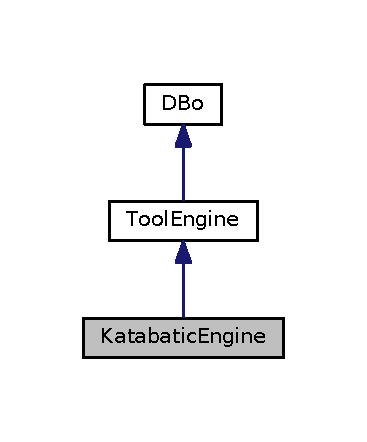
\includegraphics[width=176pt]{classKatabatic_1_1KatabaticEngine__inherit__graph}
\end{center}
\end{figure}
\subsection*{Public Types}
\begin{DoxyCompactItemize}
\item 
typedef set$<$ \textbf{ Net} $\ast$, Net\+Compare\+By\+Name $>$ \mbox{\hyperlink{classKatabatic_1_1KatabaticEngine_a92ed88f9aecd2f195089c4029fa8bcc7}{Net\+Set}}
\end{DoxyCompactItemize}
\subsection*{Public Member Functions}
\begin{DoxyCompactItemize}
\item 
bool \mbox{\hyperlink{classKatabatic_1_1KatabaticEngine_a83a7793270669d2669222eac2caa7f93}{is\+G\+Metal}} (const \textbf{ Layer} $\ast$) const
\item 
bool \mbox{\hyperlink{classKatabatic_1_1KatabaticEngine_ab6b7bc2b47ead460ac00a531451dc9cf}{is\+Chip}} () const
\item 
bool \mbox{\hyperlink{classKatabatic_1_1KatabaticEngine_a0141bff96a4778a806d4eba5d256c32a}{is\+In\+Demo\+Mode}} () const
\item 
bool \mbox{\hyperlink{classKatabatic_1_1KatabaticEngine_a9dec164d53fdee77f0f008133ecbd97f}{do\+Warn\+On\+G\+Cell\+Overload}} () const
\item 
bool \mbox{\hyperlink{classKatabatic_1_1KatabaticEngine_a6bb0ac3c0ec9720a3519d43491939f97}{do\+Destroy\+Base\+Contact}} () const
\item 
bool \mbox{\hyperlink{classKatabatic_1_1KatabaticEngine_a54d58d645317d43371f6b0bec1815e6b}{do\+Destroy\+Base\+Segment}} () const
\item 
bool \mbox{\hyperlink{classKatabatic_1_1KatabaticEngine_a867e6dbfea5e5895a01ef71c66398b26}{do\+Destroy\+Tool}} () const
\item 
virtual const \textbf{ Name} \& \mbox{\hyperlink{classKatabatic_1_1KatabaticEngine_a9e76ae5cee9320b65251387419c9432b}{get\+Name}} () const
\item 
\mbox{\hyperlink{namespaceKatabatic_ab9e409db5feff0bdbc85e90e2a029cda}{Engine\+State}} \mbox{\hyperlink{classKatabatic_1_1KatabaticEngine_a878e8b694aa243a767c2f232799ec9b3}{get\+State}} () const
\item 
unsigned int \mbox{\hyperlink{classKatabatic_1_1KatabaticEngine_a7132cd3f405dc24b3897b4396c8ecc92}{get\+Flags}} (unsigned int mask) const
\item 
Configuration $\ast$ \mbox{\hyperlink{classKatabatic_1_1KatabaticEngine_adccd6ceec2c68234d3a824ad7ae3954e}{get\+Katabatic\+Configuration}} ()
\item 
virtual Configuration $\ast$ \mbox{\hyperlink{classKatabatic_1_1KatabaticEngine_a9a7fbadfe526875680f698c76adfb128}{get\+Configuration}} ()
\item 
\textbf{ Routing\+Gauge} $\ast$ \mbox{\hyperlink{classKatabatic_1_1KatabaticEngine_a171ed6fac01ac5067d4f1b770cc419cf}{get\+Routing\+Gauge}} () const
\item 
\textbf{ Routing\+Layer\+Gauge} $\ast$ \mbox{\hyperlink{classKatabatic_1_1KatabaticEngine_a0b7c308ac7fccc21dd0401c6ce70a586}{get\+Layer\+Gauge}} (size\+\_\+t depth) const
\item 
const \textbf{ Layer} $\ast$ \mbox{\hyperlink{classKatabatic_1_1KatabaticEngine_afa7ea850397e87889733ac959833b49f}{get\+Routing\+Layer}} (size\+\_\+t depth) const
\item 
\textbf{ Layer} $\ast$ \mbox{\hyperlink{classKatabatic_1_1KatabaticEngine_a4c4549515aef37e81f2cc6537b931edc}{get\+Contact\+Layer}} (size\+\_\+t depth) const
\item 
\mbox{\hyperlink{classKatabatic_1_1GCellGrid}{G\+Cell\+Grid}} $\ast$ \mbox{\hyperlink{classKatabatic_1_1KatabaticEngine_a9a56286f633fddd702d66563de457a4a}{get\+G\+Cell\+Grid}} () const
\item 
const \mbox{\hyperlink{classKatabatic_1_1KatabaticEngine_a92ed88f9aecd2f195089c4029fa8bcc7}{Net\+Set}} \& \mbox{\hyperlink{classKatabatic_1_1KatabaticEngine_a8f661928f8f709552c8486d68ac33c55}{get\+Routing\+Nets}} () const
\item 
\textbf{ Db\+U\+::\+Unit} \mbox{\hyperlink{classKatabatic_1_1KatabaticEngine_a094b479155d3f30ec54e252c35dcffa3}{get\+Global\+Threshold}} () const
\item 
float \mbox{\hyperlink{classKatabatic_1_1KatabaticEngine_a44d2c1fbd97dd09b102b461e906367a0}{get\+Saturate\+Ratio}} () const
\item 
size\+\_\+t \mbox{\hyperlink{classKatabatic_1_1KatabaticEngine_a61977cc1fd981e7f1c6125189ed20509}{get\+Saturate\+Rp}} () const
\item 
\textbf{ Db\+U\+::\+Unit} \mbox{\hyperlink{classKatabatic_1_1KatabaticEngine_ad9072cfa6215c92c9a9842270cf677c5}{get\+Extension\+Cap}} () const
\item 
const \mbox{\hyperlink{classKatabatic_1_1ChipTools}{Chip\+Tools}} \& \mbox{\hyperlink{classKatabatic_1_1KatabaticEngine_a423f5f2214c8b9fe73da9a86b6f6d9b9}{get\+Chip\+Tools}} () const
\item 
void \mbox{\hyperlink{classKatabatic_1_1KatabaticEngine_aecbe8bdcc61024a7539de3ea932c5e06}{xml\+Write\+G\+Cell\+Grid}} (ostream \&)
\item 
void \mbox{\hyperlink{classKatabatic_1_1KatabaticEngine_a78394ac380a0fa462f268dcc2becc50e}{xml\+Write\+G\+Cell\+Grid}} (const string \&)
\item 
void \mbox{\hyperlink{classKatabatic_1_1KatabaticEngine_a2391b9bfcb773398b9661b5ac0ef1a30}{set\+State}} (\mbox{\hyperlink{namespaceKatabatic_ab9e409db5feff0bdbc85e90e2a029cda}{Engine\+State}} state)
\item 
void \mbox{\hyperlink{classKatabatic_1_1KatabaticEngine_aeb14f94914af58657a0dc2f50ec98df5}{set\+Flags}} (unsigned int)
\item 
void \mbox{\hyperlink{classKatabatic_1_1KatabaticEngine_a1a6fac115cb81db48e3ac9ffa0721bb5}{unset\+Flags}} (unsigned int)
\item 
void \mbox{\hyperlink{classKatabatic_1_1KatabaticEngine_a1bd1e0104b73d4c558b0e121002796a6}{set\+Global\+Threshold}} (\textbf{ Db\+U\+::\+Unit})
\item 
void \mbox{\hyperlink{classKatabatic_1_1KatabaticEngine_ac2b780e06975ce8a0d6ca96f20cb971f}{set\+Saturate\+Ratio}} (float)
\item 
void \mbox{\hyperlink{classKatabatic_1_1KatabaticEngine_ade227e828b8c8fbfce478e353ca3ca59}{set\+Saturate\+Rp}} (size\+\_\+t)
\item 
void \mbox{\hyperlink{classKatabatic_1_1KatabaticEngine_a2ea4b4fc379fb85a13890db451cbf93a}{print\+Measures}} (const string \&) const
\item 
void \mbox{\hyperlink{classKatabatic_1_1KatabaticEngine_a1e9bb62be35c6a415a1950c72c1964ef}{refresh}} (unsigned int flags=\mbox{\hyperlink{namespaceKatabatic_a2af2ad6b6441614038caf59d04b3b217af314588109fcc5f5ee1c42e5fd4d0ed5}{Kb\+Open\+Session}})
\item 
virtual void \mbox{\hyperlink{classKatabatic_1_1KatabaticEngine_a1b7d8ed09a198f7afd6e3ac911f6eb37}{create\+Detailed\+Grid}} ()
\item 
void \mbox{\hyperlink{classKatabatic_1_1KatabaticEngine_aaba3b9450c85634131146fb507089f2d}{make\+Power\+Rails}} ()
\item 
virtual void \mbox{\hyperlink{classKatabatic_1_1KatabaticEngine_a583925cfe4bbadcc1c24fe619debce09}{load\+Global\+Routing}} (unsigned int method)
\item 
void \mbox{\hyperlink{classKatabatic_1_1KatabaticEngine_a145b36b18fc9149980c5d6bd4bd10e0d}{slacken\+Border}} (\textbf{ Box} bb, \textbf{ Layer\+::\+Mask}, unsigned int flags)
\item 
void \mbox{\hyperlink{classKatabatic_1_1KatabaticEngine_ac40754d4a9bd0cf327b5fa088e993897}{slacken\+Block\+Ios}} (\textbf{ Instance} $\ast$core)
\item 
bool \mbox{\hyperlink{classKatabatic_1_1KatabaticEngine_ac934a049003c9d5d2380f44ff393e458}{move\+Up\+Net\+Trunk}} (\mbox{\hyperlink{classKatabatic_1_1AutoSegment}{Auto\+Segment}} $\ast$, set$<$ \textbf{ Net} $\ast$$>$ \&global\+Nets, \mbox{\hyperlink{classKatabatic_1_1GCell_aacb1c215b203bfba5729f135b3221d40}{G\+Cell\+::\+Set\+Index}} \&invalidateds)
\item 
void \mbox{\hyperlink{classKatabatic_1_1KatabaticEngine_a77833ce938a430785ba869eedbc2300c}{layer\+Assign}} (unsigned int method)
\item 
void \mbox{\hyperlink{classKatabatic_1_1KatabaticEngine_a6957a5830a4d6f1b2daf83a7d98df601}{compute\+Net\+Constraints}} (\textbf{ Net} $\ast$)
\item 
void \mbox{\hyperlink{classKatabatic_1_1KatabaticEngine_ad6b9f7d94ee4a88f12c485e48d1e644a}{to\+Optimals}} (\textbf{ Net} $\ast$)
\item 
virtual void \mbox{\hyperlink{classKatabatic_1_1KatabaticEngine_a468eddb683c04cfeea1c5124a39e1f86}{finalize\+Layout}} ()
\end{DoxyCompactItemize}
\subsection*{Static Public Member Functions}
\begin{DoxyCompactItemize}
\item 
static \mbox{\hyperlink{classKatabatic_1_1KatabaticEngine}{Katabatic\+Engine}} $\ast$ \mbox{\hyperlink{classKatabatic_1_1KatabaticEngine_ab877a64c314024602cfb04631ebfbfc4}{create}} (\textbf{ Cell} $\ast$)
\item 
static const \textbf{ Name} \& \mbox{\hyperlink{classKatabatic_1_1KatabaticEngine_a802eee6265da8d536db52d412f8a4afd}{static\+Get\+Name}} ()
\end{DoxyCompactItemize}


\subsection{Detailed Description}
The \mbox{\hyperlink{namespaceKatabatic}{Katabatic}} Tool. 

\hypertarget{classKatabatic_1_1KatabaticEngine_secEngineStates}{}\subsection{States of Katabatic\+Engine}\label{classKatabatic_1_1KatabaticEngine_secEngineStates}
During it\textquotesingle{}s lifecycle, the engine go through a serie of states. It only can go forward between states.
\begin{DoxyItemize}
\item {\bfseries Engine\+Creation} \+: just after C++ object creation until the global routing is loaded.
\item {\bfseries Engine\+Global\+Loaded} \+: {\itshape after} the global routing has been done. This state must be set by an external tool, \mbox{\hyperlink{namespaceKatabatic}{Katabatic}} cannot know by itself when the global routing has been done (see Kite).
\item {\bfseries Engine\+Active} \+: {\itshape after} the global routing has been converted into the \mbox{\hyperlink{namespaceKatabatic}{Katabatic}} data structure. At this point the tool is ready to run.
\item {\bfseries Engine\+Driving} \+: {\itshape during} the stage of stripping all the decorations the tool has added over the Hurricane data structure (mostly\+: \mbox{\hyperlink{classKatabatic_1_1AutoContact}{Auto\+Contact}} \& \mbox{\hyperlink{classKatabatic_1_1AutoSegment}{Auto\+Segment}}).
\item {\bfseries Engine\+Gutted} \+: {\itshape after} the tool decorations have been removed. The tool is now useless and can only be destroyed.
\item {\bfseries Engine\+Pre\+Destroying} \+: this special state is reached when going straight from Engine\+Active to the destructor, that is, skipping the Engine\+Driving state. That means we {\itshape do not} want to save whatever routing has been done. In that case, not only the tool decorations are destroyeds, but also the Hurricane data-\/structures they relies on (Contact, Segments).
\end{DoxyItemize}\hypertarget{classKatabatic_1_1KatabaticEngine_secEngineImpl}{}\subsection{Katabatic\+Engine Implementation Details}\label{classKatabatic_1_1KatabaticEngine_secEngineImpl}
Due to the size of the code and the fact that the main body of some methods do not need to be present in the class, the implementation of \mbox{\hyperlink{classKatabatic_1_1KatabaticEngine}{Katabatic\+Engine}} is split in several files. The list below summarize them\+:
\begin{DoxyItemize}
\item {\ttfamily Katabatic\+Engine.\+cpp} \+: the core of the class, methods that really need their bodies here.
\item {\ttfamily Power\+Rails.\+cpp} \+: utilities to construct an abstract from all the power rails through the hierarchy.
\item {\ttfamily Layer\+Assign.\+cpp} \+: layer assignement related methods and helpers.
\item {\ttfamily Load\+Gr\+By\+Net.\+cpp} \+: global routing loader, transform global routing into \mbox{\hyperlink{namespaceKatabatic}{Katabatic}} data-\/structure.
\item {\ttfamily Net\+Constraints.\+cpp} \+: compute the topological constraints of all Auto\+Segment/\+Auto\+Contact of a Net.
\item {\ttfamily Net\+Optimals.\+cpp} \+: compute the optimal positions of all \mbox{\hyperlink{classKatabatic_1_1AutoSegment}{Auto\+Segment}} of a Net. 
\end{DoxyItemize}

\subsection{Member Typedef Documentation}
\mbox{\Hypertarget{classKatabatic_1_1KatabaticEngine_a92ed88f9aecd2f195089c4029fa8bcc7}\label{classKatabatic_1_1KatabaticEngine_a92ed88f9aecd2f195089c4029fa8bcc7}} 
\index{Katabatic\+::\+Katabatic\+Engine@{Katabatic\+::\+Katabatic\+Engine}!Net\+Set@{Net\+Set}}
\index{Net\+Set@{Net\+Set}!Katabatic\+::\+Katabatic\+Engine@{Katabatic\+::\+Katabatic\+Engine}}
\subsubsection{\texorpdfstring{Net\+Set}{NetSet}}
{\footnotesize\ttfamily set$<$ \textbf{ Net} $\ast$, Net\+Compare\+By\+Name $>$ \mbox{\hyperlink{classKatabatic_1_1KatabaticEngine_a92ed88f9aecd2f195089c4029fa8bcc7}{Net\+Set}}}

Set of Net to be routed, alphabetically sorteds. 

\subsection{Member Function Documentation}
\mbox{\Hypertarget{classKatabatic_1_1KatabaticEngine_ab877a64c314024602cfb04631ebfbfc4}\label{classKatabatic_1_1KatabaticEngine_ab877a64c314024602cfb04631ebfbfc4}} 
\index{Katabatic\+::\+Katabatic\+Engine@{Katabatic\+::\+Katabatic\+Engine}!create@{create}}
\index{create@{create}!Katabatic\+::\+Katabatic\+Engine@{Katabatic\+::\+Katabatic\+Engine}}
\subsubsection{\texorpdfstring{create()}{create()}}
{\footnotesize\ttfamily \mbox{\hyperlink{classKatabatic_1_1KatabaticEngine}{Katabatic\+Engine}} $\ast$ create (\begin{DoxyParamCaption}\item[{\textbf{ Cell} $\ast$}]{cell }\end{DoxyParamCaption})\hspace{0.3cm}{\ttfamily [static]}}

Create a \mbox{\hyperlink{classKatabatic_1_1KatabaticEngine}{Katabatic\+Engine}} on {\ttfamily cell}. \mbox{\Hypertarget{classKatabatic_1_1KatabaticEngine_a802eee6265da8d536db52d412f8a4afd}\label{classKatabatic_1_1KatabaticEngine_a802eee6265da8d536db52d412f8a4afd}} 
\index{Katabatic\+::\+Katabatic\+Engine@{Katabatic\+::\+Katabatic\+Engine}!static\+Get\+Name@{static\+Get\+Name}}
\index{static\+Get\+Name@{static\+Get\+Name}!Katabatic\+::\+Katabatic\+Engine@{Katabatic\+::\+Katabatic\+Engine}}
\subsubsection{\texorpdfstring{static\+Get\+Name()}{staticGetName()}}
{\footnotesize\ttfamily const \textbf{ Name} \& static\+Get\+Name (\begin{DoxyParamCaption}{ }\end{DoxyParamCaption})\hspace{0.3cm}{\ttfamily [static]}}

{\bfseries Returns\+:} The unique string identifier for the \mbox{\hyperlink{classKatabatic_1_1KatabaticEngine}{Katabatic\+Engine}} class of Tool\+Engine. \mbox{\Hypertarget{classKatabatic_1_1KatabaticEngine_a83a7793270669d2669222eac2caa7f93}\label{classKatabatic_1_1KatabaticEngine_a83a7793270669d2669222eac2caa7f93}} 
\index{Katabatic\+::\+Katabatic\+Engine@{Katabatic\+::\+Katabatic\+Engine}!is\+G\+Metal@{is\+G\+Metal}}
\index{is\+G\+Metal@{is\+G\+Metal}!Katabatic\+::\+Katabatic\+Engine@{Katabatic\+::\+Katabatic\+Engine}}
\subsubsection{\texorpdfstring{is\+G\+Metal()}{isGMetal()}}
{\footnotesize\ttfamily bool is\+G\+Metal (\begin{DoxyParamCaption}\item[{const \textbf{ Layer} $\ast$}]{layer }\end{DoxyParamCaption}) const\hspace{0.3cm}{\ttfamily [inline]}}

{\bfseries Returns\+:} {\bfseries true} if {\ttfamily layer} is one of the special (fake) metals used to build the global routing. 

Referenced by Auto\+Segment\+::create().

\mbox{\Hypertarget{classKatabatic_1_1KatabaticEngine_ab6b7bc2b47ead460ac00a531451dc9cf}\label{classKatabatic_1_1KatabaticEngine_ab6b7bc2b47ead460ac00a531451dc9cf}} 
\index{Katabatic\+::\+Katabatic\+Engine@{Katabatic\+::\+Katabatic\+Engine}!is\+Chip@{is\+Chip}}
\index{is\+Chip@{is\+Chip}!Katabatic\+::\+Katabatic\+Engine@{Katabatic\+::\+Katabatic\+Engine}}
\subsubsection{\texorpdfstring{is\+Chip()}{isChip()}}
{\footnotesize\ttfamily bool is\+Chip (\begin{DoxyParamCaption}{ }\end{DoxyParamCaption}) const\hspace{0.3cm}{\ttfamily [inline]}}

{\bfseries Returns\+:} {\bfseries true} if the hierarchy top-\/level of the Cell matches the one of a complete design (i.\+e. pads and one core instance). 

References Chip\+Tools\+::is\+Chip().

\mbox{\Hypertarget{classKatabatic_1_1KatabaticEngine_a0141bff96a4778a806d4eba5d256c32a}\label{classKatabatic_1_1KatabaticEngine_a0141bff96a4778a806d4eba5d256c32a}} 
\index{Katabatic\+::\+Katabatic\+Engine@{Katabatic\+::\+Katabatic\+Engine}!is\+In\+Demo\+Mode@{is\+In\+Demo\+Mode}}
\index{is\+In\+Demo\+Mode@{is\+In\+Demo\+Mode}!Katabatic\+::\+Katabatic\+Engine@{Katabatic\+::\+Katabatic\+Engine}}
\subsubsection{\texorpdfstring{is\+In\+Demo\+Mode()}{isInDemoMode()}}
{\footnotesize\ttfamily bool is\+In\+Demo\+Mode (\begin{DoxyParamCaption}{ }\end{DoxyParamCaption}) const\hspace{0.3cm}{\ttfamily [inline]}}

{\bfseries Returns\+:} {\bfseries true} if the tool is in demo mode, that is suppress almost all warning and debug messages. 

Referenced by Session\+::is\+In\+Demo\+Mode().

\mbox{\Hypertarget{classKatabatic_1_1KatabaticEngine_a9dec164d53fdee77f0f008133ecbd97f}\label{classKatabatic_1_1KatabaticEngine_a9dec164d53fdee77f0f008133ecbd97f}} 
\index{Katabatic\+::\+Katabatic\+Engine@{Katabatic\+::\+Katabatic\+Engine}!do\+Warn\+On\+G\+Cell\+Overload@{do\+Warn\+On\+G\+Cell\+Overload}}
\index{do\+Warn\+On\+G\+Cell\+Overload@{do\+Warn\+On\+G\+Cell\+Overload}!Katabatic\+::\+Katabatic\+Engine@{Katabatic\+::\+Katabatic\+Engine}}
\subsubsection{\texorpdfstring{do\+Warn\+On\+G\+Cell\+Overload()}{doWarnOnGCellOverload()}}
{\footnotesize\ttfamily bool do\+Warn\+On\+G\+Cell\+Overload (\begin{DoxyParamCaption}{ }\end{DoxyParamCaption}) const\hspace{0.3cm}{\ttfamily [inline]}}

{\bfseries Returns\+:} {\bfseries true} if the tool should issue a warning when a \mbox{\hyperlink{classKatabatic_1_1GCell}{G\+Cell}} is overloaded (overload could be transient). 

Referenced by Session\+::do\+Warn\+G\+Cell\+Overload().

\mbox{\Hypertarget{classKatabatic_1_1KatabaticEngine_a6bb0ac3c0ec9720a3519d43491939f97}\label{classKatabatic_1_1KatabaticEngine_a6bb0ac3c0ec9720a3519d43491939f97}} 
\index{Katabatic\+::\+Katabatic\+Engine@{Katabatic\+::\+Katabatic\+Engine}!do\+Destroy\+Base\+Contact@{do\+Destroy\+Base\+Contact}}
\index{do\+Destroy\+Base\+Contact@{do\+Destroy\+Base\+Contact}!Katabatic\+::\+Katabatic\+Engine@{Katabatic\+::\+Katabatic\+Engine}}
\subsubsection{\texorpdfstring{do\+Destroy\+Base\+Contact()}{doDestroyBaseContact()}}
{\footnotesize\ttfamily bool do\+Destroy\+Base\+Contact (\begin{DoxyParamCaption}{ }\end{DoxyParamCaption}) const\hspace{0.3cm}{\ttfamily [inline]}}

{\bfseries Returns\+:} {\bfseries true} if the Engine\+Destroy\+Base\+Contact is set, meaning that when an \mbox{\hyperlink{classKatabatic_1_1AutoContact}{Auto\+Contact}} is destroyed, the Contact it decorates is destroyed altogether. \mbox{\Hypertarget{classKatabatic_1_1KatabaticEngine_a54d58d645317d43371f6b0bec1815e6b}\label{classKatabatic_1_1KatabaticEngine_a54d58d645317d43371f6b0bec1815e6b}} 
\index{Katabatic\+::\+Katabatic\+Engine@{Katabatic\+::\+Katabatic\+Engine}!do\+Destroy\+Base\+Segment@{do\+Destroy\+Base\+Segment}}
\index{do\+Destroy\+Base\+Segment@{do\+Destroy\+Base\+Segment}!Katabatic\+::\+Katabatic\+Engine@{Katabatic\+::\+Katabatic\+Engine}}
\subsubsection{\texorpdfstring{do\+Destroy\+Base\+Segment()}{doDestroyBaseSegment()}}
{\footnotesize\ttfamily bool do\+Destroy\+Base\+Segment (\begin{DoxyParamCaption}{ }\end{DoxyParamCaption}) const\hspace{0.3cm}{\ttfamily [inline]}}

{\bfseries Returns\+:} {\bfseries true} if the Engine\+Destroy\+Base\+Segment is set, meaning that when an \mbox{\hyperlink{classKatabatic_1_1AutoSegment}{Auto\+Segment}} is destroyed, the Segment it decorates is destroyed altogether. \mbox{\Hypertarget{classKatabatic_1_1KatabaticEngine_a867e6dbfea5e5895a01ef71c66398b26}\label{classKatabatic_1_1KatabaticEngine_a867e6dbfea5e5895a01ef71c66398b26}} 
\index{Katabatic\+::\+Katabatic\+Engine@{Katabatic\+::\+Katabatic\+Engine}!do\+Destroy\+Tool@{do\+Destroy\+Tool}}
\index{do\+Destroy\+Tool@{do\+Destroy\+Tool}!Katabatic\+::\+Katabatic\+Engine@{Katabatic\+::\+Katabatic\+Engine}}
\subsubsection{\texorpdfstring{do\+Destroy\+Tool()}{doDestroyTool()}}
{\footnotesize\ttfamily bool do\+Destroy\+Tool (\begin{DoxyParamCaption}{ }\end{DoxyParamCaption}) const\hspace{0.3cm}{\ttfamily [inline]}}

{\bfseries Returns\+:} {\bfseries true} if the tool state is beyond Engine\+State\+Gutted, that is, only waits for {\ttfamily \textbf{ destroy()}} to be called. 

References Katabatic\+::\+Engine\+Gutted.

\mbox{\Hypertarget{classKatabatic_1_1KatabaticEngine_a9e76ae5cee9320b65251387419c9432b}\label{classKatabatic_1_1KatabaticEngine_a9e76ae5cee9320b65251387419c9432b}} 
\index{Katabatic\+::\+Katabatic\+Engine@{Katabatic\+::\+Katabatic\+Engine}!get\+Name@{get\+Name}}
\index{get\+Name@{get\+Name}!Katabatic\+::\+Katabatic\+Engine@{Katabatic\+::\+Katabatic\+Engine}}
\subsubsection{\texorpdfstring{get\+Name()}{getName()}}
{\footnotesize\ttfamily const \textbf{ Name} \& get\+Name (\begin{DoxyParamCaption}{ }\end{DoxyParamCaption}) const\hspace{0.3cm}{\ttfamily [virtual]}}

{\bfseries Returns\+:} The unique string identifier for the \mbox{\hyperlink{classKatabatic_1_1KatabaticEngine}{Katabatic\+Engine}} class of Tool\+Engine. 

Implements \textbf{ Tool\+Engine}.

\mbox{\Hypertarget{classKatabatic_1_1KatabaticEngine_a878e8b694aa243a767c2f232799ec9b3}\label{classKatabatic_1_1KatabaticEngine_a878e8b694aa243a767c2f232799ec9b3}} 
\index{Katabatic\+::\+Katabatic\+Engine@{Katabatic\+::\+Katabatic\+Engine}!get\+State@{get\+State}}
\index{get\+State@{get\+State}!Katabatic\+::\+Katabatic\+Engine@{Katabatic\+::\+Katabatic\+Engine}}
\subsubsection{\texorpdfstring{get\+State()}{getState()}}
{\footnotesize\ttfamily \mbox{\hyperlink{namespaceKatabatic_ab9e409db5feff0bdbc85e90e2a029cda}{Engine\+State}} get\+State (\begin{DoxyParamCaption}{ }\end{DoxyParamCaption}) const\hspace{0.3cm}{\ttfamily [inline]}}

{\bfseries Returns\+:} The state the tool is currently in. \mbox{\Hypertarget{classKatabatic_1_1KatabaticEngine_a7132cd3f405dc24b3897b4396c8ecc92}\label{classKatabatic_1_1KatabaticEngine_a7132cd3f405dc24b3897b4396c8ecc92}} 
\index{Katabatic\+::\+Katabatic\+Engine@{Katabatic\+::\+Katabatic\+Engine}!get\+Flags@{get\+Flags}}
\index{get\+Flags@{get\+Flags}!Katabatic\+::\+Katabatic\+Engine@{Katabatic\+::\+Katabatic\+Engine}}
\subsubsection{\texorpdfstring{get\+Flags()}{getFlags()}}
{\footnotesize\ttfamily unsigned int get\+Flags (\begin{DoxyParamCaption}\item[{unsigned int}]{mask }\end{DoxyParamCaption}) const\hspace{0.3cm}{\ttfamily [inline]}}

{\bfseries Returns\+:} The {\itshape anded} combination of the tool flags and {\ttfamily mask}. \mbox{\Hypertarget{classKatabatic_1_1KatabaticEngine_adccd6ceec2c68234d3a824ad7ae3954e}\label{classKatabatic_1_1KatabaticEngine_adccd6ceec2c68234d3a824ad7ae3954e}} 
\index{Katabatic\+::\+Katabatic\+Engine@{Katabatic\+::\+Katabatic\+Engine}!get\+Katabatic\+Configuration@{get\+Katabatic\+Configuration}}
\index{get\+Katabatic\+Configuration@{get\+Katabatic\+Configuration}!Katabatic\+::\+Katabatic\+Engine@{Katabatic\+::\+Katabatic\+Engine}}
\subsubsection{\texorpdfstring{get\+Katabatic\+Configuration()}{getKatabaticConfiguration()}}
{\footnotesize\ttfamily Configuration $\ast$ get\+Katabatic\+Configuration (\begin{DoxyParamCaption}{ }\end{DoxyParamCaption})\hspace{0.3cm}{\ttfamily [inline]}}

{\bfseries Returns\+:} The Configuration of \mbox{\hyperlink{namespaceKatabatic}{Katabatic}}. In this class it is redundant with \mbox{\hyperlink{classKatabatic_1_1KatabaticEngine_a9a7fbadfe526875680f698c76adfb128}{get\+Configuration()}}, but may be useful in derived classes. \mbox{\Hypertarget{classKatabatic_1_1KatabaticEngine_a9a7fbadfe526875680f698c76adfb128}\label{classKatabatic_1_1KatabaticEngine_a9a7fbadfe526875680f698c76adfb128}} 
\index{Katabatic\+::\+Katabatic\+Engine@{Katabatic\+::\+Katabatic\+Engine}!get\+Configuration@{get\+Configuration}}
\index{get\+Configuration@{get\+Configuration}!Katabatic\+::\+Katabatic\+Engine@{Katabatic\+::\+Katabatic\+Engine}}
\subsubsection{\texorpdfstring{get\+Configuration()}{getConfiguration()}}
{\footnotesize\ttfamily Configuration $\ast$ get\+Configuration (\begin{DoxyParamCaption}{ }\end{DoxyParamCaption})\hspace{0.3cm}{\ttfamily [virtual]}}

{\bfseries Returns\+:} The Configuration of the current Tool\+Engine. \mbox{\Hypertarget{classKatabatic_1_1KatabaticEngine_a171ed6fac01ac5067d4f1b770cc419cf}\label{classKatabatic_1_1KatabaticEngine_a171ed6fac01ac5067d4f1b770cc419cf}} 
\index{Katabatic\+::\+Katabatic\+Engine@{Katabatic\+::\+Katabatic\+Engine}!get\+Routing\+Gauge@{get\+Routing\+Gauge}}
\index{get\+Routing\+Gauge@{get\+Routing\+Gauge}!Katabatic\+::\+Katabatic\+Engine@{Katabatic\+::\+Katabatic\+Engine}}
\subsubsection{\texorpdfstring{get\+Routing\+Gauge()}{getRoutingGauge()}}
{\footnotesize\ttfamily \textbf{ Routing\+Gauge} $\ast$ get\+Routing\+Gauge (\begin{DoxyParamCaption}{ }\end{DoxyParamCaption}) const\hspace{0.3cm}{\ttfamily [inline]}}

{\bfseries Returns\+:} The Routing\+Gauge (Configuration shortcut). \mbox{\Hypertarget{classKatabatic_1_1KatabaticEngine_a0b7c308ac7fccc21dd0401c6ce70a586}\label{classKatabatic_1_1KatabaticEngine_a0b7c308ac7fccc21dd0401c6ce70a586}} 
\index{Katabatic\+::\+Katabatic\+Engine@{Katabatic\+::\+Katabatic\+Engine}!get\+Layer\+Gauge@{get\+Layer\+Gauge}}
\index{get\+Layer\+Gauge@{get\+Layer\+Gauge}!Katabatic\+::\+Katabatic\+Engine@{Katabatic\+::\+Katabatic\+Engine}}
\subsubsection{\texorpdfstring{get\+Layer\+Gauge()}{getLayerGauge()}}
{\footnotesize\ttfamily \textbf{ Routing\+Layer\+Gauge} $\ast$ get\+Layer\+Gauge (\begin{DoxyParamCaption}\item[{size\+\_\+t}]{depth }\end{DoxyParamCaption}) const\hspace{0.3cm}{\ttfamily [inline]}}

{\bfseries Returns\+:} The Routing\+Layer\+Gauge associated to {\ttfamily depth} (Configuration shortcut). \mbox{\Hypertarget{classKatabatic_1_1KatabaticEngine_afa7ea850397e87889733ac959833b49f}\label{classKatabatic_1_1KatabaticEngine_afa7ea850397e87889733ac959833b49f}} 
\index{Katabatic\+::\+Katabatic\+Engine@{Katabatic\+::\+Katabatic\+Engine}!get\+Routing\+Layer@{get\+Routing\+Layer}}
\index{get\+Routing\+Layer@{get\+Routing\+Layer}!Katabatic\+::\+Katabatic\+Engine@{Katabatic\+::\+Katabatic\+Engine}}
\subsubsection{\texorpdfstring{get\+Routing\+Layer()}{getRoutingLayer()}}
{\footnotesize\ttfamily const \textbf{ Layer} $\ast$ get\+Routing\+Layer (\begin{DoxyParamCaption}\item[{size\+\_\+t}]{depth }\end{DoxyParamCaption}) const\hspace{0.3cm}{\ttfamily [inline]}}

{\bfseries Returns\+:} The routing Layer associated to {\ttfamily depth} (Configuration shortcut). \mbox{\Hypertarget{classKatabatic_1_1KatabaticEngine_a4c4549515aef37e81f2cc6537b931edc}\label{classKatabatic_1_1KatabaticEngine_a4c4549515aef37e81f2cc6537b931edc}} 
\index{Katabatic\+::\+Katabatic\+Engine@{Katabatic\+::\+Katabatic\+Engine}!get\+Contact\+Layer@{get\+Contact\+Layer}}
\index{get\+Contact\+Layer@{get\+Contact\+Layer}!Katabatic\+::\+Katabatic\+Engine@{Katabatic\+::\+Katabatic\+Engine}}
\subsubsection{\texorpdfstring{get\+Contact\+Layer()}{getContactLayer()}}
{\footnotesize\ttfamily \textbf{ Layer} $\ast$ get\+Contact\+Layer (\begin{DoxyParamCaption}\item[{size\+\_\+t}]{depth }\end{DoxyParamCaption}) const\hspace{0.3cm}{\ttfamily [inline]}}

{\bfseries Returns\+:} The contact Layer associated to {\ttfamily depth} (Configuration shortcut). \mbox{\Hypertarget{classKatabatic_1_1KatabaticEngine_a9a56286f633fddd702d66563de457a4a}\label{classKatabatic_1_1KatabaticEngine_a9a56286f633fddd702d66563de457a4a}} 
\index{Katabatic\+::\+Katabatic\+Engine@{Katabatic\+::\+Katabatic\+Engine}!get\+G\+Cell\+Grid@{get\+G\+Cell\+Grid}}
\index{get\+G\+Cell\+Grid@{get\+G\+Cell\+Grid}!Katabatic\+::\+Katabatic\+Engine@{Katabatic\+::\+Katabatic\+Engine}}
\subsubsection{\texorpdfstring{get\+G\+Cell\+Grid()}{getGCellGrid()}}
{\footnotesize\ttfamily \mbox{\hyperlink{classKatabatic_1_1GCellGrid}{G\+Cell\+Grid}} $\ast$ get\+G\+Cell\+Grid (\begin{DoxyParamCaption}{ }\end{DoxyParamCaption}) const\hspace{0.3cm}{\ttfamily [inline]}}

{\bfseries Returns\+:} The \mbox{\hyperlink{classKatabatic_1_1GCellGrid}{G\+Cell\+Grid}}. 

Referenced by G\+Cell\+Topology\+::do\+Rp\+\_\+\+Access\+Pad(), G\+Cell\+Topology\+::do\+Rp\+\_\+\+Auto\+Contacts(), and anonymous\+\_\+namespace\{\+Load\+Gr\+By\+Net.\+cpp\}\+::single\+G\+Cell().

\mbox{\Hypertarget{classKatabatic_1_1KatabaticEngine_a8f661928f8f709552c8486d68ac33c55}\label{classKatabatic_1_1KatabaticEngine_a8f661928f8f709552c8486d68ac33c55}} 
\index{Katabatic\+::\+Katabatic\+Engine@{Katabatic\+::\+Katabatic\+Engine}!get\+Routing\+Nets@{get\+Routing\+Nets}}
\index{get\+Routing\+Nets@{get\+Routing\+Nets}!Katabatic\+::\+Katabatic\+Engine@{Katabatic\+::\+Katabatic\+Engine}}
\subsubsection{\texorpdfstring{get\+Routing\+Nets()}{getRoutingNets()}}
{\footnotesize\ttfamily const \mbox{\hyperlink{classKatabatic_1_1KatabaticEngine_a92ed88f9aecd2f195089c4029fa8bcc7}{Net\+Set}} \& get\+Routing\+Nets (\begin{DoxyParamCaption}{ }\end{DoxyParamCaption}) const\hspace{0.3cm}{\ttfamily [inline]}}

{\bfseries Returns\+:} The set of nets to be routeds. \mbox{\Hypertarget{classKatabatic_1_1KatabaticEngine_a094b479155d3f30ec54e252c35dcffa3}\label{classKatabatic_1_1KatabaticEngine_a094b479155d3f30ec54e252c35dcffa3}} 
\index{Katabatic\+::\+Katabatic\+Engine@{Katabatic\+::\+Katabatic\+Engine}!get\+Global\+Threshold@{get\+Global\+Threshold}}
\index{get\+Global\+Threshold@{get\+Global\+Threshold}!Katabatic\+::\+Katabatic\+Engine@{Katabatic\+::\+Katabatic\+Engine}}
\subsubsection{\texorpdfstring{get\+Global\+Threshold()}{getGlobalThreshold()}}
{\footnotesize\ttfamily \textbf{ Db\+U\+::\+Unit} get\+Global\+Threshold (\begin{DoxyParamCaption}{ }\end{DoxyParamCaption}) const\hspace{0.3cm}{\ttfamily [inline]}}

{\bfseries Returns\+:} The length above which a global wire is moved up in the layer assignment stage (Configuration shortcut). \mbox{\Hypertarget{classKatabatic_1_1KatabaticEngine_a44d2c1fbd97dd09b102b461e906367a0}\label{classKatabatic_1_1KatabaticEngine_a44d2c1fbd97dd09b102b461e906367a0}} 
\index{Katabatic\+::\+Katabatic\+Engine@{Katabatic\+::\+Katabatic\+Engine}!get\+Saturate\+Ratio@{get\+Saturate\+Ratio}}
\index{get\+Saturate\+Ratio@{get\+Saturate\+Ratio}!Katabatic\+::\+Katabatic\+Engine@{Katabatic\+::\+Katabatic\+Engine}}
\subsubsection{\texorpdfstring{get\+Saturate\+Ratio()}{getSaturateRatio()}}
{\footnotesize\ttfamily float get\+Saturate\+Ratio (\begin{DoxyParamCaption}{ }\end{DoxyParamCaption}) const\hspace{0.3cm}{\ttfamily [inline]}}

{\bfseries Returns\+:} The ratio above which a \mbox{\hyperlink{classKatabatic_1_1GCell}{G\+Cell}} is considered to be saturated (Configuration shortcut). 

Referenced by Session\+::get\+Saturate\+Ratio().

\mbox{\Hypertarget{classKatabatic_1_1KatabaticEngine_a61977cc1fd981e7f1c6125189ed20509}\label{classKatabatic_1_1KatabaticEngine_a61977cc1fd981e7f1c6125189ed20509}} 
\index{Katabatic\+::\+Katabatic\+Engine@{Katabatic\+::\+Katabatic\+Engine}!get\+Saturate\+Rp@{get\+Saturate\+Rp}}
\index{get\+Saturate\+Rp@{get\+Saturate\+Rp}!Katabatic\+::\+Katabatic\+Engine@{Katabatic\+::\+Katabatic\+Engine}}
\subsubsection{\texorpdfstring{get\+Saturate\+Rp()}{getSaturateRp()}}
{\footnotesize\ttfamily size\+\_\+t get\+Saturate\+Rp (\begin{DoxyParamCaption}{ }\end{DoxyParamCaption}) const\hspace{0.3cm}{\ttfamily [inline]}}

{\bfseries Returns\+:} The number of Routing\+Pad above which a \mbox{\hyperlink{classKatabatic_1_1GCell}{G\+Cell}} is saturated, causing extras global segments to be moved up. (Configuration shortcut). 

Referenced by Session\+::get\+Saturate\+Rp().

\mbox{\Hypertarget{classKatabatic_1_1KatabaticEngine_ad9072cfa6215c92c9a9842270cf677c5}\label{classKatabatic_1_1KatabaticEngine_ad9072cfa6215c92c9a9842270cf677c5}} 
\index{Katabatic\+::\+Katabatic\+Engine@{Katabatic\+::\+Katabatic\+Engine}!get\+Extension\+Cap@{get\+Extension\+Cap}}
\index{get\+Extension\+Cap@{get\+Extension\+Cap}!Katabatic\+::\+Katabatic\+Engine@{Katabatic\+::\+Katabatic\+Engine}}
\subsubsection{\texorpdfstring{get\+Extension\+Cap()}{getExtensionCap()}}
{\footnotesize\ttfamily \textbf{ Db\+U\+::\+Unit} get\+Extension\+Cap (\begin{DoxyParamCaption}{ }\end{DoxyParamCaption}) const\hspace{0.3cm}{\ttfamily [inline]}}

{\bfseries Returns\+:} The wires extension cap, same for all layers for the time beeing (Configuration shortcut). \mbox{\Hypertarget{classKatabatic_1_1KatabaticEngine_a423f5f2214c8b9fe73da9a86b6f6d9b9}\label{classKatabatic_1_1KatabaticEngine_a423f5f2214c8b9fe73da9a86b6f6d9b9}} 
\index{Katabatic\+::\+Katabatic\+Engine@{Katabatic\+::\+Katabatic\+Engine}!get\+Chip\+Tools@{get\+Chip\+Tools}}
\index{get\+Chip\+Tools@{get\+Chip\+Tools}!Katabatic\+::\+Katabatic\+Engine@{Katabatic\+::\+Katabatic\+Engine}}
\subsubsection{\texorpdfstring{get\+Chip\+Tools()}{getChipTools()}}
{\footnotesize\ttfamily const \mbox{\hyperlink{classKatabatic_1_1ChipTools}{Chip\+Tools}} \& get\+Chip\+Tools (\begin{DoxyParamCaption}{ }\end{DoxyParamCaption}) const\hspace{0.3cm}{\ttfamily [inline]}}

{\bfseries Returns\+:} The chip tools (for whole designs). 

Referenced by Katabatic\+Engine\+::create\+Detailed\+Grid().

\mbox{\Hypertarget{classKatabatic_1_1KatabaticEngine_aecbe8bdcc61024a7539de3ea932c5e06}\label{classKatabatic_1_1KatabaticEngine_aecbe8bdcc61024a7539de3ea932c5e06}} 
\index{Katabatic\+::\+Katabatic\+Engine@{Katabatic\+::\+Katabatic\+Engine}!xml\+Write\+G\+Cell\+Grid@{xml\+Write\+G\+Cell\+Grid}}
\index{xml\+Write\+G\+Cell\+Grid@{xml\+Write\+G\+Cell\+Grid}!Katabatic\+::\+Katabatic\+Engine@{Katabatic\+::\+Katabatic\+Engine}}
\subsubsection{\texorpdfstring{xml\+Write\+G\+Cell\+Grid()}{xmlWriteGCellGrid()}\hspace{0.1cm}{\footnotesize\ttfamily [1/2]}}
{\footnotesize\ttfamily void xml\+Write\+G\+Cell\+Grid (\begin{DoxyParamCaption}\item[{ostream \&}]{o }\end{DoxyParamCaption})}

Write in a stream all informations on the G\+Cells in X\+ML format. 

Referenced by Katabatic\+Engine\+::xml\+Write\+G\+Cell\+Grid().

\mbox{\Hypertarget{classKatabatic_1_1KatabaticEngine_a78394ac380a0fa462f268dcc2becc50e}\label{classKatabatic_1_1KatabaticEngine_a78394ac380a0fa462f268dcc2becc50e}} 
\index{Katabatic\+::\+Katabatic\+Engine@{Katabatic\+::\+Katabatic\+Engine}!xml\+Write\+G\+Cell\+Grid@{xml\+Write\+G\+Cell\+Grid}}
\index{xml\+Write\+G\+Cell\+Grid@{xml\+Write\+G\+Cell\+Grid}!Katabatic\+::\+Katabatic\+Engine@{Katabatic\+::\+Katabatic\+Engine}}
\subsubsection{\texorpdfstring{xml\+Write\+G\+Cell\+Grid()}{xmlWriteGCellGrid()}\hspace{0.1cm}{\footnotesize\ttfamily [2/2]}}
{\footnotesize\ttfamily void xml\+Write\+G\+Cell\+Grid (\begin{DoxyParamCaption}\item[{const string \&}]{file\+Name }\end{DoxyParamCaption})}

Write in a file all informations on the G\+Cells in X\+ML format. 

References Katabatic\+Engine\+::xml\+Write\+G\+Cell\+Grid().

\mbox{\Hypertarget{classKatabatic_1_1KatabaticEngine_a2391b9bfcb773398b9661b5ac0ef1a30}\label{classKatabatic_1_1KatabaticEngine_a2391b9bfcb773398b9661b5ac0ef1a30}} 
\index{Katabatic\+::\+Katabatic\+Engine@{Katabatic\+::\+Katabatic\+Engine}!set\+State@{set\+State}}
\index{set\+State@{set\+State}!Katabatic\+::\+Katabatic\+Engine@{Katabatic\+::\+Katabatic\+Engine}}
\subsubsection{\texorpdfstring{set\+State()}{setState()}}
{\footnotesize\ttfamily void set\+State (\begin{DoxyParamCaption}\item[{\mbox{\hyperlink{namespaceKatabatic_ab9e409db5feff0bdbc85e90e2a029cda}{Engine\+State}}}]{state }\end{DoxyParamCaption})\hspace{0.3cm}{\ttfamily [inline]}}

Force the state of the tool. Must be used with caution, as no sanity checks are performeds. This method is normally invoked from inside the \mbox{\hyperlink{classKatabatic_1_1KatabaticEngine}{Katabatic\+Engine}} various methods. \mbox{\Hypertarget{classKatabatic_1_1KatabaticEngine_aeb14f94914af58657a0dc2f50ec98df5}\label{classKatabatic_1_1KatabaticEngine_aeb14f94914af58657a0dc2f50ec98df5}} 
\index{Katabatic\+::\+Katabatic\+Engine@{Katabatic\+::\+Katabatic\+Engine}!set\+Flags@{set\+Flags}}
\index{set\+Flags@{set\+Flags}!Katabatic\+::\+Katabatic\+Engine@{Katabatic\+::\+Katabatic\+Engine}}
\subsubsection{\texorpdfstring{set\+Flags()}{setFlags()}}
{\footnotesize\ttfamily void set\+Flags (\begin{DoxyParamCaption}\item[{unsigned int}]{flags }\end{DoxyParamCaption})\hspace{0.3cm}{\ttfamily [inline]}}

Set the flags given in {\ttfamily flags}. 

Referenced by Session\+::set\+Katabatic\+Flags().

\mbox{\Hypertarget{classKatabatic_1_1KatabaticEngine_a1a6fac115cb81db48e3ac9ffa0721bb5}\label{classKatabatic_1_1KatabaticEngine_a1a6fac115cb81db48e3ac9ffa0721bb5}} 
\index{Katabatic\+::\+Katabatic\+Engine@{Katabatic\+::\+Katabatic\+Engine}!unset\+Flags@{unset\+Flags}}
\index{unset\+Flags@{unset\+Flags}!Katabatic\+::\+Katabatic\+Engine@{Katabatic\+::\+Katabatic\+Engine}}
\subsubsection{\texorpdfstring{unset\+Flags()}{unsetFlags()}}
{\footnotesize\ttfamily void unset\+Flags (\begin{DoxyParamCaption}\item[{unsigned int}]{flags }\end{DoxyParamCaption})\hspace{0.3cm}{\ttfamily [inline]}}

Reset the flags given in {\ttfamily flags}. \mbox{\Hypertarget{classKatabatic_1_1KatabaticEngine_a1bd1e0104b73d4c558b0e121002796a6}\label{classKatabatic_1_1KatabaticEngine_a1bd1e0104b73d4c558b0e121002796a6}} 
\index{Katabatic\+::\+Katabatic\+Engine@{Katabatic\+::\+Katabatic\+Engine}!set\+Global\+Threshold@{set\+Global\+Threshold}}
\index{set\+Global\+Threshold@{set\+Global\+Threshold}!Katabatic\+::\+Katabatic\+Engine@{Katabatic\+::\+Katabatic\+Engine}}
\subsubsection{\texorpdfstring{set\+Global\+Threshold()}{setGlobalThreshold()}}
{\footnotesize\ttfamily void set\+Global\+Threshold (\begin{DoxyParamCaption}\item[{\textbf{ Db\+U\+::\+Unit}}]{threshold }\end{DoxyParamCaption})\hspace{0.3cm}{\ttfamily [inline]}}

(Configuration shortcut). \mbox{\Hypertarget{classKatabatic_1_1KatabaticEngine_ac2b780e06975ce8a0d6ca96f20cb971f}\label{classKatabatic_1_1KatabaticEngine_ac2b780e06975ce8a0d6ca96f20cb971f}} 
\index{Katabatic\+::\+Katabatic\+Engine@{Katabatic\+::\+Katabatic\+Engine}!set\+Saturate\+Ratio@{set\+Saturate\+Ratio}}
\index{set\+Saturate\+Ratio@{set\+Saturate\+Ratio}!Katabatic\+::\+Katabatic\+Engine@{Katabatic\+::\+Katabatic\+Engine}}
\subsubsection{\texorpdfstring{set\+Saturate\+Ratio()}{setSaturateRatio()}}
{\footnotesize\ttfamily void set\+Saturate\+Ratio (\begin{DoxyParamCaption}\item[{float}]{ratio }\end{DoxyParamCaption})\hspace{0.3cm}{\ttfamily [inline]}}

(Configuration shortcut). \mbox{\Hypertarget{classKatabatic_1_1KatabaticEngine_ade227e828b8c8fbfce478e353ca3ca59}\label{classKatabatic_1_1KatabaticEngine_ade227e828b8c8fbfce478e353ca3ca59}} 
\index{Katabatic\+::\+Katabatic\+Engine@{Katabatic\+::\+Katabatic\+Engine}!set\+Saturate\+Rp@{set\+Saturate\+Rp}}
\index{set\+Saturate\+Rp@{set\+Saturate\+Rp}!Katabatic\+::\+Katabatic\+Engine@{Katabatic\+::\+Katabatic\+Engine}}
\subsubsection{\texorpdfstring{set\+Saturate\+Rp()}{setSaturateRp()}}
{\footnotesize\ttfamily void set\+Saturate\+Rp (\begin{DoxyParamCaption}\item[{size\+\_\+t}]{threshold }\end{DoxyParamCaption})\hspace{0.3cm}{\ttfamily [inline]}}

(Configuration shortcut). \mbox{\Hypertarget{classKatabatic_1_1KatabaticEngine_a2ea4b4fc379fb85a13890db451cbf93a}\label{classKatabatic_1_1KatabaticEngine_a2ea4b4fc379fb85a13890db451cbf93a}} 
\index{Katabatic\+::\+Katabatic\+Engine@{Katabatic\+::\+Katabatic\+Engine}!print\+Measures@{print\+Measures}}
\index{print\+Measures@{print\+Measures}!Katabatic\+::\+Katabatic\+Engine@{Katabatic\+::\+Katabatic\+Engine}}
\subsubsection{\texorpdfstring{print\+Measures()}{printMeasures()}}
{\footnotesize\ttfamily void print\+Measures (\begin{DoxyParamCaption}\item[{const string \&}]{tag }\end{DoxyParamCaption}) const}

Print memory \& time measurement on \`{}\`{}cmess1\`{}\`{}. If {\ttfamily tag} is not empty, also adds the measurement to the internal table (with {\ttfamily tag} as label). 

Referenced by Katabatic\+Engine\+::finalize\+Layout().

\mbox{\Hypertarget{classKatabatic_1_1KatabaticEngine_a1e9bb62be35c6a415a1950c72c1964ef}\label{classKatabatic_1_1KatabaticEngine_a1e9bb62be35c6a415a1950c72c1964ef}} 
\index{Katabatic\+::\+Katabatic\+Engine@{Katabatic\+::\+Katabatic\+Engine}!refresh@{refresh}}
\index{refresh@{refresh}!Katabatic\+::\+Katabatic\+Engine@{Katabatic\+::\+Katabatic\+Engine}}
\subsubsection{\texorpdfstring{refresh()}{refresh()}}
{\footnotesize\ttfamily void refresh (\begin{DoxyParamCaption}\item[{unsigned int}]{flags = {\ttfamily \mbox{\hyperlink{namespaceKatabatic_a2af2ad6b6441614038caf59d04b3b217af314588109fcc5f5ee1c42e5fd4d0ed5}{Kb\+Open\+Session}}} }\end{DoxyParamCaption})}

In case the tool is associated with a graphic display, trigger a full redraw of the Cell. Slow the router but allow to see work in progress... If {\ttfamily flags} {\itshape do not} contains {\ttfamily Kb\+Open\+Session} the refresh operation will not be enclosed inside it\textquotesingle{}s own session. This assumes that a session is already opened. 

References G\+Cell\+Grid\+::update\+Contacts().

\mbox{\Hypertarget{classKatabatic_1_1KatabaticEngine_a1b7d8ed09a198f7afd6e3ac911f6eb37}\label{classKatabatic_1_1KatabaticEngine_a1b7d8ed09a198f7afd6e3ac911f6eb37}} 
\index{Katabatic\+::\+Katabatic\+Engine@{Katabatic\+::\+Katabatic\+Engine}!create\+Detailed\+Grid@{create\+Detailed\+Grid}}
\index{create\+Detailed\+Grid@{create\+Detailed\+Grid}!Katabatic\+::\+Katabatic\+Engine@{Katabatic\+::\+Katabatic\+Engine}}
\subsubsection{\texorpdfstring{create\+Detailed\+Grid()}{createDetailedGrid()}}
{\footnotesize\ttfamily void create\+Detailed\+Grid (\begin{DoxyParamCaption}{ }\end{DoxyParamCaption})\hspace{0.3cm}{\ttfamily [virtual]}}

Allocate the \mbox{\hyperlink{classKatabatic_1_1GCellGrid}{G\+Cell\+Grid}}. 

References G\+Cell\+Grid\+::create(), Katabatic\+Engine\+::get\+Chip\+Tools(), Base\+Grid\+::get\+Columns(), Grid$<$ G\+Cell\+T $>$\+::get\+G\+Cells\+Column(), Grid$<$ G\+Cell\+T $>$\+::get\+G\+Cells\+Row(), Base\+Grid\+::get\+Rows(), Chip\+Tools\+::is\+Chip(), and Session\+::revalidate().

\mbox{\Hypertarget{classKatabatic_1_1KatabaticEngine_aaba3b9450c85634131146fb507089f2d}\label{classKatabatic_1_1KatabaticEngine_aaba3b9450c85634131146fb507089f2d}} 
\index{Katabatic\+::\+Katabatic\+Engine@{Katabatic\+::\+Katabatic\+Engine}!make\+Power\+Rails@{make\+Power\+Rails}}
\index{make\+Power\+Rails@{make\+Power\+Rails}!Katabatic\+::\+Katabatic\+Engine@{Katabatic\+::\+Katabatic\+Engine}}
\subsubsection{\texorpdfstring{make\+Power\+Rails()}{makePowerRails()}}
{\footnotesize\ttfamily void make\+Power\+Rails (\begin{DoxyParamCaption}{ }\end{DoxyParamCaption})}

Detect all the aligned segments of same width that compose power rails, unificate them and copy them at the design top level. \mbox{\Hypertarget{classKatabatic_1_1KatabaticEngine_a583925cfe4bbadcc1c24fe619debce09}\label{classKatabatic_1_1KatabaticEngine_a583925cfe4bbadcc1c24fe619debce09}} 
\index{Katabatic\+::\+Katabatic\+Engine@{Katabatic\+::\+Katabatic\+Engine}!load\+Global\+Routing@{load\+Global\+Routing}}
\index{load\+Global\+Routing@{load\+Global\+Routing}!Katabatic\+::\+Katabatic\+Engine@{Katabatic\+::\+Katabatic\+Engine}}
\subsubsection{\texorpdfstring{load\+Global\+Routing()}{loadGlobalRouting()}}
{\footnotesize\ttfamily void load\+Global\+Routing (\begin{DoxyParamCaption}\item[{unsigned int}]{method }\end{DoxyParamCaption})\hspace{0.3cm}{\ttfamily [virtual]}}


\begin{DoxyParams}{Parameters}
{\em method} & the loading algorithm \\
\hline
{\em nets} & the set of nets to route.\\
\hline
\end{DoxyParams}
Convert the global routing into the initial detailed routing. For the time beeing, only one loading algorithm is available\+: {\itshape net by net} (Engine\+Load\+Gr\+By\+Net). Only Net given in {\ttfamily nets} are routeds. If {\ttfamily nets} is empty then all ordinary nets are routeds. In either cases the set of nets to route is pruned from any power, ground or clock signals.

\begin{DoxyParagraph}{Remark\+: The tool state must be {\bfseries Engine\+Global\+Loaded} {\itshape before} calling this method}
and will be set to {\bfseries Engine\+Active} on exit. 
\end{DoxyParagraph}


References Katabatic\+::\+Engine\+Active, and Katabatic\+::\+Engine\+Global\+Loaded.

\mbox{\Hypertarget{classKatabatic_1_1KatabaticEngine_a145b36b18fc9149980c5d6bd4bd10e0d}\label{classKatabatic_1_1KatabaticEngine_a145b36b18fc9149980c5d6bd4bd10e0d}} 
\index{Katabatic\+::\+Katabatic\+Engine@{Katabatic\+::\+Katabatic\+Engine}!slacken\+Border@{slacken\+Border}}
\index{slacken\+Border@{slacken\+Border}!Katabatic\+::\+Katabatic\+Engine@{Katabatic\+::\+Katabatic\+Engine}}
\subsubsection{\texorpdfstring{slacken\+Border()}{slackenBorder()}}
{\footnotesize\ttfamily void slacken\+Border (\begin{DoxyParamCaption}\item[{\textbf{ Box}}]{bb,  }\item[{\textbf{ Layer\+::\+Mask}}]{mask,  }\item[{unsigned int}]{flags }\end{DoxyParamCaption})}


\begin{DoxyParams}{Parameters}
{\em bb} & The bounding box, defines the edges. \\
\hline
{\em mask} & Consider only layers that are fully included in that mask. \\
\hline
{\em flags} & Consider only segment in that direction.\\
\hline
\end{DoxyParams}
Perform a preventive break on all global segments going through the {\itshape vertical} left and right edges of the {\ttfamily bb} box. The set of global segments to be broken could be further restricted using {\ttfamily mask} and {\ttfamily flags}.

The Semantic of {\ttfamily flags} is not clear, must review the code more closely. 

References Box\+::get\+X\+Max(), Box\+::get\+X\+Min(), Box\+::get\+Y\+Max(), and Box\+::get\+Y\+Min().

\mbox{\Hypertarget{classKatabatic_1_1KatabaticEngine_ac40754d4a9bd0cf327b5fa088e993897}\label{classKatabatic_1_1KatabaticEngine_ac40754d4a9bd0cf327b5fa088e993897}} 
\index{Katabatic\+::\+Katabatic\+Engine@{Katabatic\+::\+Katabatic\+Engine}!slacken\+Block\+Ios@{slacken\+Block\+Ios}}
\index{slacken\+Block\+Ios@{slacken\+Block\+Ios}!Katabatic\+::\+Katabatic\+Engine@{Katabatic\+::\+Katabatic\+Engine}}
\subsubsection{\texorpdfstring{slacken\+Block\+Ios()}{slackenBlockIos()}}
{\footnotesize\ttfamily void slacken\+Block\+Ios (\begin{DoxyParamCaption}\item[{\textbf{ Instance} $\ast$}]{core }\end{DoxyParamCaption})}

Perform a preventive break on horizontal segments in the \mbox{\hyperlink{classKatabatic_1_1GCell}{G\+Cell}} immediatly {\itshape outside} the instance {\ttfamily core} area in the routing layer of index {\ttfamily 1}.

This method is too much hardwired to the {\ttfamily Sx\+Lib} gauge. It\textquotesingle{}s effect is to break all {\bfseries M\+E\+T\+A\+L2} outside the core (in a chip). 

References Entity\+::get\+Bounding\+Box(), Instance\+::get\+Name(), Constant\+::\+Horizontal, and Box\+::inflate().

\mbox{\Hypertarget{classKatabatic_1_1KatabaticEngine_ac934a049003c9d5d2380f44ff393e458}\label{classKatabatic_1_1KatabaticEngine_ac934a049003c9d5d2380f44ff393e458}} 
\index{Katabatic\+::\+Katabatic\+Engine@{Katabatic\+::\+Katabatic\+Engine}!move\+Up\+Net\+Trunk@{move\+Up\+Net\+Trunk}}
\index{move\+Up\+Net\+Trunk@{move\+Up\+Net\+Trunk}!Katabatic\+::\+Katabatic\+Engine@{Katabatic\+::\+Katabatic\+Engine}}
\subsubsection{\texorpdfstring{move\+Up\+Net\+Trunk()}{moveUpNetTrunk()}}
{\footnotesize\ttfamily bool move\+Up\+Net\+Trunk (\begin{DoxyParamCaption}\item[{\mbox{\hyperlink{classKatabatic_1_1AutoSegment}{Auto\+Segment}} $\ast$}]{seed,  }\item[{set$<$ \textbf{ Net} $\ast$$>$ \&}]{global\+Nets,  }\item[{\mbox{\hyperlink{classKatabatic_1_1GCell_aacb1c215b203bfba5729f135b3221d40}{G\+Cell\+::\+Set\+Index}} \&}]{invalidateds }\end{DoxyParamCaption})}


\begin{DoxyParams}{Parameters}
{\em seed} & The \mbox{\hyperlink{classKatabatic_1_1AutoSegment}{Auto\+Segment}} to take the net from. \\
\hline
{\em global\+Nets} & The set of nets that has been moved up. \\
\hline
{\em invalidateds} & The set of G\+Cells that have been invalidated. {\bfseries Returns\+:} {\bfseries true} if the net trunk have been moved up.\\
\hline
\end{DoxyParams}
Try to move up a whole net trunk. The net is supplied through the {\ttfamily seed} argument (the segment that triggers the move). If the net is actually moved up, it is added to {\ttfamily global\+Nets} and all G\+Cells that have been invalidateds are added to {\ttfamily invalidateds}.

An individual \mbox{\hyperlink{classKatabatic_1_1AutoSegment}{Auto\+Segment}} of the net is moved up if it\textquotesingle{}s length is greater that {\ttfamily 150} lambdas, that is, three times the side of a \mbox{\hyperlink{classKatabatic_1_1GCell}{G\+Cell}}. This is hard-\/wired and should be parametrized in the future. \mbox{\Hypertarget{classKatabatic_1_1KatabaticEngine_a77833ce938a430785ba869eedbc2300c}\label{classKatabatic_1_1KatabaticEngine_a77833ce938a430785ba869eedbc2300c}} 
\index{Katabatic\+::\+Katabatic\+Engine@{Katabatic\+::\+Katabatic\+Engine}!layer\+Assign@{layer\+Assign}}
\index{layer\+Assign@{layer\+Assign}!Katabatic\+::\+Katabatic\+Engine@{Katabatic\+::\+Katabatic\+Engine}}
\subsubsection{\texorpdfstring{layer\+Assign()}{layerAssign()}}
{\footnotesize\ttfamily void layer\+Assign (\begin{DoxyParamCaption}\item[{unsigned int}]{method }\end{DoxyParamCaption})}

Perform the layer assignment. The global routing loading stage uses only the two bottom most layers, this method spread them on all the availables routing layers, according to \mbox{\hyperlink{classKatabatic_1_1GCell}{G\+Cell}} and Routing\+Pad density criterions.

Two algorithms are availables\+:
\begin{DoxyItemize}
\item {\bfseries Engine\+Layer\+Assign\+By\+Length} \+: the global wires are moved up one by one.
\item {\bfseries Engine\+Layer\+Assign\+By\+Trunk} \+: if one global wire of a net is to be moved up, then all the global trunk of the net is moved along. This methods gives the best results for now. 
\end{DoxyItemize}\mbox{\Hypertarget{classKatabatic_1_1KatabaticEngine_a6957a5830a4d6f1b2daf83a7d98df601}\label{classKatabatic_1_1KatabaticEngine_a6957a5830a4d6f1b2daf83a7d98df601}} 
\index{Katabatic\+::\+Katabatic\+Engine@{Katabatic\+::\+Katabatic\+Engine}!compute\+Net\+Constraints@{compute\+Net\+Constraints}}
\index{compute\+Net\+Constraints@{compute\+Net\+Constraints}!Katabatic\+::\+Katabatic\+Engine@{Katabatic\+::\+Katabatic\+Engine}}
\subsubsection{\texorpdfstring{compute\+Net\+Constraints()}{computeNetConstraints()}}
{\footnotesize\ttfamily void compute\+Net\+Constraints (\begin{DoxyParamCaption}\item[{\textbf{ Net} $\ast$}]{net }\end{DoxyParamCaption})}

Compute the box constraints on Auto\+Contacts (and therefore those applied to Auto\+Segments). Constraints comes from Auto\+Contacts anchoreds on Routing\+Pads and transmitted through \mbox{\hyperlink{classKatabatic_1_1AutoContactHTee}{Auto\+Contact\+H\+Tee}} or \mbox{\hyperlink{classKatabatic_1_1AutoContactVTee}{Auto\+Contact\+V\+Tee}}. Constraints are applied to all Auto\+Contacts of an aligned set.

\begin{DoxyParagraph}{Remark\+: The {\ttfamily net} must have been canonized before this function to be called. }

\end{DoxyParagraph}
\mbox{\Hypertarget{classKatabatic_1_1KatabaticEngine_ad6b9f7d94ee4a88f12c485e48d1e644a}\label{classKatabatic_1_1KatabaticEngine_ad6b9f7d94ee4a88f12c485e48d1e644a}} 
\index{Katabatic\+::\+Katabatic\+Engine@{Katabatic\+::\+Katabatic\+Engine}!to\+Optimals@{to\+Optimals}}
\index{to\+Optimals@{to\+Optimals}!Katabatic\+::\+Katabatic\+Engine@{Katabatic\+::\+Katabatic\+Engine}}
\subsubsection{\texorpdfstring{to\+Optimals()}{toOptimals()}}
{\footnotesize\ttfamily void to\+Optimals (\begin{DoxyParamCaption}\item[{\textbf{ Net} $\ast$}]{net }\end{DoxyParamCaption})}

Move all \mbox{\hyperlink{classKatabatic_1_1AutoSegment}{Auto\+Segment}} of {\ttfamily net} so that their axis are inside their optimals interval. If a \mbox{\hyperlink{classKatabatic_1_1AutoSegment}{Auto\+Segment}} is already inside the interval is not moved, otherwise it is put on the nearest bound of the optimal interval. \mbox{\Hypertarget{classKatabatic_1_1KatabaticEngine_a468eddb683c04cfeea1c5124a39e1f86}\label{classKatabatic_1_1KatabaticEngine_a468eddb683c04cfeea1c5124a39e1f86}} 
\index{Katabatic\+::\+Katabatic\+Engine@{Katabatic\+::\+Katabatic\+Engine}!finalize\+Layout@{finalize\+Layout}}
\index{finalize\+Layout@{finalize\+Layout}!Katabatic\+::\+Katabatic\+Engine@{Katabatic\+::\+Katabatic\+Engine}}
\subsubsection{\texorpdfstring{finalize\+Layout()}{finalizeLayout()}}
{\footnotesize\ttfamily void finalize\+Layout (\begin{DoxyParamCaption}{ }\end{DoxyParamCaption})\hspace{0.3cm}{\ttfamily [virtual]}}

Transform the \mbox{\hyperlink{namespaceKatabatic}{Katabatic}} wires into the Hurricane data-\/structure. Mostly by removing the Auto\+Segment/\+Auto\+Contact {\itshape without} removing their Hurricane conterparts. May also fill gaps that may have appeared.

\begin{DoxyParagraph}{Remark\+: The tool state must be {\bfseries Engine\+Active} {\itshape before} calling this method}
and will be set to {\bfseries Engine\+Gutted} on exit. 
\end{DoxyParagraph}


References Katabatic\+::\+Engine\+Driving, Katabatic\+::\+Engine\+Gutted, and Katabatic\+Engine\+::print\+Measures().



The documentation for this class was generated from the following files\+:\begin{DoxyCompactItemize}
\item 
Katabatic\+Engine.\+h\item 
Chip\+Tools.\+cpp\item 
Load\+Gr\+By\+Net.\+cpp\item 
Katabatic\+Engine.\+cpp\item 
Katabatic\+Engine.\+dox\end{DoxyCompactItemize}

\hypertarget{classKatabatic_1_1GCell_1_1Key}{}\section{G\+Cell\+:\+:Key Class Reference}
\label{classKatabatic_1_1GCell_1_1Key}\index{G\+Cell\+::\+Key@{G\+Cell\+::\+Key}}


\mbox{\hyperlink{classKatabatic_1_1GCell}{G\+Cell}} \mbox{\hyperlink{classKatabatic_1_1GCell_1_1Key}{Key}} -\/ Density Cache.  


\subsection*{Public Member Functions}
\begin{DoxyCompactItemize}
\item 
\mbox{\hyperlink{classKatabatic_1_1GCell_1_1Key_a6efdb05badcc81d3d3013ce4730bbe6e}{Key}} (\mbox{\hyperlink{classKatabatic_1_1GCell}{G\+Cell}} $\ast$, unsigned int depth)
\item 
float \mbox{\hyperlink{classKatabatic_1_1GCell_1_1Key_a9f45c741b4c738e833fe66fe125592b7}{get\+Density}} () const
\item 
\mbox{\hyperlink{classKatabatic_1_1GCell}{G\+Cell}} $\ast$ \mbox{\hyperlink{classKatabatic_1_1GCell_1_1Key_a819cf639562a031a1e2e061fe1293d66}{get\+G\+Cell}} () const
\item 
void \mbox{\hyperlink{classKatabatic_1_1GCell_1_1Key_a1b9cfb06a645d2b0d93024bc6ff82e9e}{update}} (unsigned int depth)
\end{DoxyCompactItemize}


\subsection{Detailed Description}
\mbox{\hyperlink{classKatabatic_1_1GCell}{G\+Cell}} \mbox{\hyperlink{classKatabatic_1_1GCell_1_1Key}{Key}} -\/ Density Cache. 

This class is used to create a \mbox{\hyperlink{classKatabatic_1_1GCell}{G\+Cell}} internal cache on density, mainly to be used by \mbox{\hyperlink{classKatabatic_1_1GCellDensitySet}{G\+Cell\+Density\+Set}}. 

\subsection{Constructor \& Destructor Documentation}
\mbox{\Hypertarget{classKatabatic_1_1GCell_1_1Key_a6efdb05badcc81d3d3013ce4730bbe6e}\label{classKatabatic_1_1GCell_1_1Key_a6efdb05badcc81d3d3013ce4730bbe6e}} 
\index{Katabatic\+::\+G\+Cell\+::\+Key@{Katabatic\+::\+G\+Cell\+::\+Key}!Key@{Key}}
\index{Key@{Key}!Katabatic\+::\+G\+Cell\+::\+Key@{Katabatic\+::\+G\+Cell\+::\+Key}}
\subsubsection{\texorpdfstring{Key()}{Key()}}
{\footnotesize\ttfamily \mbox{\hyperlink{classKatabatic_1_1GCell_1_1Key}{Key}} (\begin{DoxyParamCaption}\item[{\mbox{\hyperlink{classKatabatic_1_1GCell}{G\+Cell}} $\ast$}]{owner,  }\item[{unsigned int}]{depth }\end{DoxyParamCaption})\hspace{0.3cm}{\ttfamily [inline]}}


\begin{DoxyParams}{Parameters}
{\em owner} & The \mbox{\hyperlink{classKatabatic_1_1GCell}{G\+Cell}} owning the key. \\
\hline
{\em depth} & The layer {\ttfamily depth} of the density to use.\\
\hline
\end{DoxyParams}
\mbox{\hyperlink{classKatabatic_1_1GCell_1_1Key}{Key}} constructor, with an initial value for the cached density. 

\subsection{Member Function Documentation}
\mbox{\Hypertarget{classKatabatic_1_1GCell_1_1Key_a9f45c741b4c738e833fe66fe125592b7}\label{classKatabatic_1_1GCell_1_1Key_a9f45c741b4c738e833fe66fe125592b7}} 
\index{Katabatic\+::\+G\+Cell\+::\+Key@{Katabatic\+::\+G\+Cell\+::\+Key}!get\+Density@{get\+Density}}
\index{get\+Density@{get\+Density}!Katabatic\+::\+G\+Cell\+::\+Key@{Katabatic\+::\+G\+Cell\+::\+Key}}
\subsubsection{\texorpdfstring{get\+Density()}{getDensity()}}
{\footnotesize\ttfamily float get\+Density (\begin{DoxyParamCaption}{ }\end{DoxyParamCaption}) const\hspace{0.3cm}{\ttfamily [inline]}}

{\bfseries Returns\+:} The value of the cached density. \mbox{\Hypertarget{classKatabatic_1_1GCell_1_1Key_a819cf639562a031a1e2e061fe1293d66}\label{classKatabatic_1_1GCell_1_1Key_a819cf639562a031a1e2e061fe1293d66}} 
\index{Katabatic\+::\+G\+Cell\+::\+Key@{Katabatic\+::\+G\+Cell\+::\+Key}!get\+G\+Cell@{get\+G\+Cell}}
\index{get\+G\+Cell@{get\+G\+Cell}!Katabatic\+::\+G\+Cell\+::\+Key@{Katabatic\+::\+G\+Cell\+::\+Key}}
\subsubsection{\texorpdfstring{get\+G\+Cell()}{getGCell()}}
{\footnotesize\ttfamily \mbox{\hyperlink{classKatabatic_1_1GCell}{G\+Cell}} $\ast$ get\+G\+Cell (\begin{DoxyParamCaption}{ }\end{DoxyParamCaption}) const\hspace{0.3cm}{\ttfamily [inline]}}

{\bfseries Returns\+:} The owning \mbox{\hyperlink{classKatabatic_1_1GCell}{G\+Cell}}. \mbox{\Hypertarget{classKatabatic_1_1GCell_1_1Key_a1b9cfb06a645d2b0d93024bc6ff82e9e}\label{classKatabatic_1_1GCell_1_1Key_a1b9cfb06a645d2b0d93024bc6ff82e9e}} 
\index{Katabatic\+::\+G\+Cell\+::\+Key@{Katabatic\+::\+G\+Cell\+::\+Key}!update@{update}}
\index{update@{update}!Katabatic\+::\+G\+Cell\+::\+Key@{Katabatic\+::\+G\+Cell\+::\+Key}}
\subsubsection{\texorpdfstring{update()}{update()}}
{\footnotesize\ttfamily void update (\begin{DoxyParamCaption}\item[{unsigned int}]{depth }\end{DoxyParamCaption})\hspace{0.3cm}{\ttfamily [inline]}}

{\bfseries Returns\+:} Update the density 

Referenced by G\+Cell\+::update\+Key().



The documentation for this class was generated from the following files\+:\begin{DoxyCompactItemize}
\item 
G\+Cell.\+h\item 
G\+Cell.\+dox\end{DoxyCompactItemize}

\hypertarget{classKatabatic_1_1LocatorHelper}{}\section{Locator\+Helper Class Reference}
\label{classKatabatic_1_1LocatorHelper}\index{Locator\+Helper@{Locator\+Helper}}


Locator Helper Collection\textquotesingle{}s Locators.  


\subsection*{Public Member Functions}
\begin{DoxyCompactItemize}
\item 
\mbox{\hyperlink{classKatabatic_1_1LocatorHelper_af44c2fcc73d387e3e3b5c334f25b070b}{Locator\+Helper}} (\mbox{\hyperlink{classKatabatic_1_1AutoContact}{Auto\+Contact}} $\ast$, unsigned int flags=0)
\item 
bool \mbox{\hyperlink{classKatabatic_1_1LocatorHelper_a5bc2a781be2586924afce4e4a4ea6697}{is\+Valid}} () const
\item 
\mbox{\hyperlink{classKatabatic_1_1AutoSegment}{Auto\+Segment}} $\ast$ \mbox{\hyperlink{classKatabatic_1_1LocatorHelper_ad0f8becc4187c833b6f6c5f902f8aaa5}{get\+Segment}} () const
\item 
void \mbox{\hyperlink{classKatabatic_1_1LocatorHelper_a1be98ae64bededebc29a04f257024ebe}{progress}} ()
\end{DoxyCompactItemize}


\subsection{Detailed Description}
Locator Helper Collection\textquotesingle{}s Locators. 

Provide a small uniform walktough over the Auto\+Segments anchored on Auto\+Contacts. The {\ttfamily flags} argument allows to choose between direction and include perpandiculars (in that case all segments are processeds).\hypertarget{classKatabatic_1_1LocatorHelper_secLocHelperImplementation}{}\subsection{Implementation Details}\label{classKatabatic_1_1LocatorHelper_secLocHelperImplementation}
As, at most, two horizontals and two verticals may be anchored on any \mbox{\hyperlink{classKatabatic_1_1AutoContact}{Auto\+Contact}} subtype, the locator helper perform a walk through a virtual table of 4 elements. The two first are the horizontals, the two last the verticals. The meaning of this index is consistent whith the {\ttfamily index} argument of \mbox{\hyperlink{classKatabatic_1_1AutoContact_a50531ded68cc5206fe104b8d8bf3bd87}{Auto\+Contact\+::get\+Segment()}}. When a segment is not present in an \mbox{\hyperlink{classKatabatic_1_1AutoContact}{Auto\+Contact}}, the {\ttfamily \mbox{\hyperlink{classKatabatic_1_1LocatorHelper_ad0f8becc4187c833b6f6c5f902f8aaa5}{get\+Segment()}}} returns {\ttfamily N\+U\+LL} and the \mbox{\hyperlink{classKatabatic_1_1LocatorHelper_a1be98ae64bededebc29a04f257024ebe}{Locator\+Helper\+::progress()}} function will skip it.

The private methods\+:
\begin{DoxyItemize}
\item {\ttfamily Locator\+Helper\+::\+\_\+min()} 
\item {\ttfamily Locator\+Helper\+::\+\_\+max()} 
\end{DoxyItemize}

Computes the bounds of {\ttfamily \+\_\+index} according to the value of {\ttfamily \+\_\+flags\+:} 
\begin{DoxyItemize}
\item {\ttfamily Kb\+Horizontal} \+: {\ttfamily 0} to less than {\ttfamily 2}.
\item {\ttfamily Kb\+Vertical} \+: {\ttfamily 2} to less than {\ttfamily 4}.
\item {\ttfamily Kb\+Horizontal$\vert$\+Kb\+Vertical} \+: {\ttfamily 0} to less than {\ttfamily 4}. 
\end{DoxyItemize}

\subsection{Constructor \& Destructor Documentation}
\mbox{\Hypertarget{classKatabatic_1_1LocatorHelper_af44c2fcc73d387e3e3b5c334f25b070b}\label{classKatabatic_1_1LocatorHelper_af44c2fcc73d387e3e3b5c334f25b070b}} 
\index{Katabatic\+::\+Locator\+Helper@{Katabatic\+::\+Locator\+Helper}!Locator\+Helper@{Locator\+Helper}}
\index{Locator\+Helper@{Locator\+Helper}!Katabatic\+::\+Locator\+Helper@{Katabatic\+::\+Locator\+Helper}}
\subsubsection{\texorpdfstring{Locator\+Helper()}{LocatorHelper()}}
{\footnotesize\ttfamily \mbox{\hyperlink{classKatabatic_1_1LocatorHelper}{Locator\+Helper}} (\begin{DoxyParamCaption}\item[{\mbox{\hyperlink{classKatabatic_1_1AutoContact}{Auto\+Contact}} $\ast$}]{contact,  }\item[{unsigned int}]{flags = {\ttfamily 0} }\end{DoxyParamCaption})\hspace{0.3cm}{\ttfamily [inline]}}

Create a helper to iterate over the Auto\+Segments anchored on {\ttfamily contact}. The {\ttfamily flags} arguments allow to select\+:
\begin{DoxyItemize}
\item The direction\+: \mbox{\hyperlink{namespaceKatabatic_a2af2ad6b6441614038caf59d04b3b217a1a9045673c5d3c30b067100f1440ae1b}{Katabatic\+::\+Kb\+Horizontal}} or \mbox{\hyperlink{namespaceKatabatic_a2af2ad6b6441614038caf59d04b3b217a284cad95203a27172838b09e396e3590}{Katabatic\+::\+Kb\+Vertical}}.
\item Perpandicular inclusion\+: \mbox{\hyperlink{namespaceKatabatic_a2af2ad6b6441614038caf59d04b3b217ae2d033c8f78b61468c827de8db5fe839}{Katabatic\+::\+Kb\+With\+Perpands}}.
\end{DoxyItemize}

When setting Kb\+With\+Perpands, all the segments will be iterated over. It may seems a somewhat contorted way of doing things, the reason is the ability to share (an pass) flags directly between different functions. 

References Auto\+Contact\+::get\+Segment(), and Locator\+Helper\+::progress().



\subsection{Member Function Documentation}
\mbox{\Hypertarget{classKatabatic_1_1LocatorHelper_a5bc2a781be2586924afce4e4a4ea6697}\label{classKatabatic_1_1LocatorHelper_a5bc2a781be2586924afce4e4a4ea6697}} 
\index{Katabatic\+::\+Locator\+Helper@{Katabatic\+::\+Locator\+Helper}!is\+Valid@{is\+Valid}}
\index{is\+Valid@{is\+Valid}!Katabatic\+::\+Locator\+Helper@{Katabatic\+::\+Locator\+Helper}}
\subsubsection{\texorpdfstring{is\+Valid()}{isValid()}}
{\footnotesize\ttfamily bool is\+Valid (\begin{DoxyParamCaption}{ }\end{DoxyParamCaption}) const\hspace{0.3cm}{\ttfamily [inline]}}

{\bfseries Returns\+:} {\bfseries true} if there is an \mbox{\hyperlink{classKatabatic_1_1AutoSegment}{Auto\+Segment}} to be processed. \mbox{\Hypertarget{classKatabatic_1_1LocatorHelper_ad0f8becc4187c833b6f6c5f902f8aaa5}\label{classKatabatic_1_1LocatorHelper_ad0f8becc4187c833b6f6c5f902f8aaa5}} 
\index{Katabatic\+::\+Locator\+Helper@{Katabatic\+::\+Locator\+Helper}!get\+Segment@{get\+Segment}}
\index{get\+Segment@{get\+Segment}!Katabatic\+::\+Locator\+Helper@{Katabatic\+::\+Locator\+Helper}}
\subsubsection{\texorpdfstring{get\+Segment()}{getSegment()}}
{\footnotesize\ttfamily \mbox{\hyperlink{classKatabatic_1_1AutoSegment}{Auto\+Segment}} $\ast$ get\+Segment (\begin{DoxyParamCaption}{ }\end{DoxyParamCaption}) const\hspace{0.3cm}{\ttfamily [inline]}}

{\bfseries Returns\+:} The current \mbox{\hyperlink{classKatabatic_1_1AutoSegment}{Auto\+Segment}}. {\ttfamily N\+U\+LL} if the loop is over. 

References Auto\+Contact\+::get\+Segment().

\mbox{\Hypertarget{classKatabatic_1_1LocatorHelper_a1be98ae64bededebc29a04f257024ebe}\label{classKatabatic_1_1LocatorHelper_a1be98ae64bededebc29a04f257024ebe}} 
\index{Katabatic\+::\+Locator\+Helper@{Katabatic\+::\+Locator\+Helper}!progress@{progress}}
\index{progress@{progress}!Katabatic\+::\+Locator\+Helper@{Katabatic\+::\+Locator\+Helper}}
\subsubsection{\texorpdfstring{progress()}{progress()}}
{\footnotesize\ttfamily void progress (\begin{DoxyParamCaption}{ }\end{DoxyParamCaption})\hspace{0.3cm}{\ttfamily [inline]}}

{\bfseries Returns\+:} Go to the next \mbox{\hyperlink{classKatabatic_1_1AutoSegment}{Auto\+Segment}}. 

References Auto\+Contact\+::get\+Segment().



Referenced by Locator\+Helper\+::\+Locator\+Helper().



The documentation for this class was generated from the following files\+:\begin{DoxyCompactItemize}
\item 
Auto\+Contact.\+h\item 
Auto\+Contact.\+dox\end{DoxyCompactItemize}

\hypertarget{classKatabatic_1_1Observable}{}\section{Observable Class Reference}
\label{classKatabatic_1_1Observable}\index{Observable@{Observable}}


\mbox{\hyperlink{classKatabatic_1_1Observer}{Observer}} Design Pattern, Subject part.  


\subsection*{Public Member Functions}
\begin{DoxyCompactItemize}
\item 
\mbox{\hyperlink{classKatabatic_1_1Observable_a6438e92e07db169a97ed3eba36788dc4}{Observable}} ()
\item 
{\footnotesize template$<$typename T $>$ }\\T $\ast$ \mbox{\hyperlink{classKatabatic_1_1Observable_acc0b7276e09628f2b101ecf751aacd2a}{get\+Observer}} ()
\item 
void \mbox{\hyperlink{classKatabatic_1_1Observable_a783fda85eeabe9c660881f236f162767}{add\+Observer}} (\mbox{\hyperlink{classKatabatic_1_1BaseObserver}{Base\+Observer}} $\ast$)
\item 
void \mbox{\hyperlink{classKatabatic_1_1Observable_acaa5a7fc7fa631e3006a42006d753f43}{remove\+Observer}} (\mbox{\hyperlink{classKatabatic_1_1BaseObserver}{Base\+Observer}} $\ast$)
\item 
void \mbox{\hyperlink{classKatabatic_1_1Observable_a52e577fb0c4f2e3650928334fb621c2f}{notify}} (unsigned int flags)
\end{DoxyCompactItemize}


\subsection{Detailed Description}
\mbox{\hyperlink{classKatabatic_1_1Observer}{Observer}} Design Pattern, Subject part. 

\mbox{\hyperlink{classKatabatic_1_1Observable}{Observable}} is the implementation of the {\itshape subject} part of the \mbox{\hyperlink{classKatabatic_1_1Observer}{Observer}} design pattern. For the time beeing it\textquotesingle{}s a simplificated version that allows only one \mbox{\hyperlink{classKatabatic_1_1Observer}{Observer}} to watch the subject.

\mbox{\hyperlink{classKatabatic_1_1Observable}{Observable}} is designed to be an attribute of the subject, not one of it\textquotesingle{}s base class.

This implantation is completly generic and has nothing specific to \mbox{\hyperlink{namespaceKatabatic}{Katabatic}}. It may be moved sometimes in Hurricane at Property level in \textbf{ Hurricane\+::\+D\+Bo}.

{\bfseries Note to Myself\+:} \mbox{\hyperlink{classKatabatic_1_1Observer}{Observer}} pattern is the one behind signal/slots. 

\subsection{Constructor \& Destructor Documentation}
\mbox{\Hypertarget{classKatabatic_1_1Observable_a6438e92e07db169a97ed3eba36788dc4}\label{classKatabatic_1_1Observable_a6438e92e07db169a97ed3eba36788dc4}} 
\index{Katabatic\+::\+Observable@{Katabatic\+::\+Observable}!Observable@{Observable}}
\index{Observable@{Observable}!Katabatic\+::\+Observable@{Katabatic\+::\+Observable}}
\subsubsection{\texorpdfstring{Observable()}{Observable()}}
{\footnotesize\ttfamily \mbox{\hyperlink{classKatabatic_1_1Observable}{Observable}} (\begin{DoxyParamCaption}{ }\end{DoxyParamCaption})\hspace{0.3cm}{\ttfamily [inline]}}

Default and only constructor. The copy constructor is disabled (made private and unimplemented). 

\subsection{Member Function Documentation}
\mbox{\Hypertarget{classKatabatic_1_1Observable_acc0b7276e09628f2b101ecf751aacd2a}\label{classKatabatic_1_1Observable_acc0b7276e09628f2b101ecf751aacd2a}} 
\index{Katabatic\+::\+Observable@{Katabatic\+::\+Observable}!get\+Observer@{get\+Observer}}
\index{get\+Observer@{get\+Observer}!Katabatic\+::\+Observable@{Katabatic\+::\+Observable}}
\subsubsection{\texorpdfstring{get\+Observer()}{getObserver()}}
{\footnotesize\ttfamily T $\ast$ get\+Observer (\begin{DoxyParamCaption}{ }\end{DoxyParamCaption})\hspace{0.3cm}{\ttfamily [inline]}}

{\bfseries Returns\+:} The (only) observer, {\ttfamily N\+U\+LL} if there is none. It is the object of which the \mbox{\hyperlink{classKatabatic_1_1Observer}{Observer}} is an attribute, that is, it\textquotesingle{}s {\itshape owner}, and not the \mbox{\hyperlink{classKatabatic_1_1Observer}{Observer}} itself which is returned. \mbox{\Hypertarget{classKatabatic_1_1Observable_a783fda85eeabe9c660881f236f162767}\label{classKatabatic_1_1Observable_a783fda85eeabe9c660881f236f162767}} 
\index{Katabatic\+::\+Observable@{Katabatic\+::\+Observable}!add\+Observer@{add\+Observer}}
\index{add\+Observer@{add\+Observer}!Katabatic\+::\+Observable@{Katabatic\+::\+Observable}}
\subsubsection{\texorpdfstring{add\+Observer()}{addObserver()}}
{\footnotesize\ttfamily void add\+Observer (\begin{DoxyParamCaption}\item[{\mbox{\hyperlink{classKatabatic_1_1BaseObserver}{Base\+Observer}} $\ast$}]{observer }\end{DoxyParamCaption})\hspace{0.3cm}{\ttfamily [inline]}}

Adds an observer. If more than one is added, throw an error. \mbox{\Hypertarget{classKatabatic_1_1Observable_acaa5a7fc7fa631e3006a42006d753f43}\label{classKatabatic_1_1Observable_acaa5a7fc7fa631e3006a42006d753f43}} 
\index{Katabatic\+::\+Observable@{Katabatic\+::\+Observable}!remove\+Observer@{remove\+Observer}}
\index{remove\+Observer@{remove\+Observer}!Katabatic\+::\+Observable@{Katabatic\+::\+Observable}}
\subsubsection{\texorpdfstring{remove\+Observer()}{removeObserver()}}
{\footnotesize\ttfamily void remove\+Observer (\begin{DoxyParamCaption}\item[{\mbox{\hyperlink{classKatabatic_1_1BaseObserver}{Base\+Observer}} $\ast$}]{observer }\end{DoxyParamCaption})\hspace{0.3cm}{\ttfamily [inline]}}

Removes an observer. If the observer do not belong to this observable, throw an exception. \mbox{\Hypertarget{classKatabatic_1_1Observable_a52e577fb0c4f2e3650928334fb621c2f}\label{classKatabatic_1_1Observable_a52e577fb0c4f2e3650928334fb621c2f}} 
\index{Katabatic\+::\+Observable@{Katabatic\+::\+Observable}!notify@{notify}}
\index{notify@{notify}!Katabatic\+::\+Observable@{Katabatic\+::\+Observable}}
\subsubsection{\texorpdfstring{notify()}{notify()}}
{\footnotesize\ttfamily void notify (\begin{DoxyParamCaption}\item[{unsigned int}]{flags }\end{DoxyParamCaption})\hspace{0.3cm}{\ttfamily [inline]}}

Used by the subject to signal a change in it\textquotesingle{}s state to the observers. The {\ttfamily flags} parameter can be used to indicates what kind of change is occuring. Values for {\ttfamily flags} are defined between the subject and the observers. 

References Base\+Observer\+::notify().



Referenced by Auto\+Segment\+::\+\_\+invalidate(), Auto\+Segment\+::\+\_\+post\+Create(), Auto\+Segment\+::\+\_\+pre\+Destroy(), and Auto\+Segment\+::revalidate().



The documentation for this class was generated from the following files\+:\begin{DoxyCompactItemize}
\item 
Observer.\+h\item 
Observer.\+dox\end{DoxyCompactItemize}

\hypertarget{classKatabatic_1_1Observer}{}\section{Observer$<$ T $>$ Class Template Reference}
\label{classKatabatic_1_1Observer}\index{Observer$<$ T $>$@{Observer$<$ T $>$}}


\mbox{\hyperlink{classKatabatic_1_1Observer}{Observer}} Design Pattern, \mbox{\hyperlink{classKatabatic_1_1Observer}{Observer}} part.  




Inheritance diagram for Observer$<$ T $>$\+:\nopagebreak
\begin{figure}[H]
\begin{center}
\leavevmode
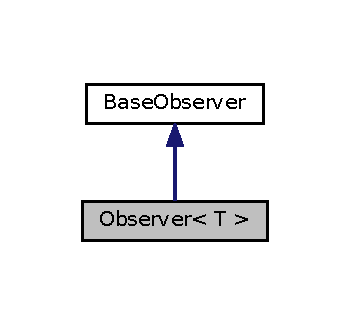
\includegraphics[width=168pt]{classKatabatic_1_1Observer__inherit__graph}
\end{center}
\end{figure}
\subsection*{Public Member Functions}
\begin{DoxyCompactItemize}
\item 
\mbox{\hyperlink{classKatabatic_1_1Observer_ab05ec12517c51952960dd4f324499b44}{Observer}} (const T $\ast$owner)
\item 
T $\ast$ \mbox{\hyperlink{classKatabatic_1_1Observer_ac29b8f99d632058c95784fd7233b8474}{get\+Owner}} () const
\end{DoxyCompactItemize}


\subsection{Detailed Description}
\subsubsection*{template$<$typename T$>$\newline
class Katabatic\+::\+Observer$<$ T $>$}

\mbox{\hyperlink{classKatabatic_1_1Observer}{Observer}} Design Pattern, \mbox{\hyperlink{classKatabatic_1_1Observer}{Observer}} part. 

{\bfseries First, a warning about names\+:} although this class is named \mbox{\hyperlink{classKatabatic_1_1Observer}{Observer}}, it is intended to be an attribute nested inside the whole object which is indeed, the true \mbox{\hyperlink{classKatabatic_1_1Observer}{Observer}}. This nesting object is called, most of the time the {\bfseries owner} in the following. But sometimes, for simplification it may also be called the \mbox{\hyperlink{classKatabatic_1_1Observer}{Observer}}.\hypertarget{classKatabatic_1_1Observer_secImplObserver}{}\subsection{Observer Implementation Notes}\label{classKatabatic_1_1Observer_secImplObserver}
To retrieve the {\itshape owner} from the \mbox{\hyperlink{classKatabatic_1_1Observer}{Observer}} attribute, we uses the offset from the attribute in the {\itshape owner}. This offset is computed once and for all the first time the template constructor is called. 

\subsection{Constructor \& Destructor Documentation}
\mbox{\Hypertarget{classKatabatic_1_1Observer_ab05ec12517c51952960dd4f324499b44}\label{classKatabatic_1_1Observer_ab05ec12517c51952960dd4f324499b44}} 
\index{Katabatic\+::\+Observer@{Katabatic\+::\+Observer}!Observer@{Observer}}
\index{Observer@{Observer}!Katabatic\+::\+Observer@{Katabatic\+::\+Observer}}
\subsubsection{\texorpdfstring{Observer()}{Observer()}}
{\footnotesize\ttfamily \mbox{\hyperlink{classKatabatic_1_1Observer}{Observer}} (\begin{DoxyParamCaption}\item[{const T $\ast$}]{owner }\end{DoxyParamCaption})\hspace{0.3cm}{\ttfamily [inline]}}

The owner of the oberver is needed to compute, on the first creation only, the offset of the \mbox{\hyperlink{classKatabatic_1_1Observer}{Observer}} attribute inside the {\ttfamily owner} complete object. 

\subsection{Member Function Documentation}
\mbox{\Hypertarget{classKatabatic_1_1Observer_ac29b8f99d632058c95784fd7233b8474}\label{classKatabatic_1_1Observer_ac29b8f99d632058c95784fd7233b8474}} 
\index{Katabatic\+::\+Observer@{Katabatic\+::\+Observer}!get\+Owner@{get\+Owner}}
\index{get\+Owner@{get\+Owner}!Katabatic\+::\+Observer@{Katabatic\+::\+Observer}}
\subsubsection{\texorpdfstring{get\+Owner()}{getOwner()}}
{\footnotesize\ttfamily T $\ast$ get\+Owner (\begin{DoxyParamCaption}{ }\end{DoxyParamCaption}) const\hspace{0.3cm}{\ttfamily [inline]}}

{\bfseries Returns\+:} The owner of the observer. 

The documentation for this class was generated from the following files\+:\begin{DoxyCompactItemize}
\item 
Observer.\+h\item 
Observer.\+dox\end{DoxyCompactItemize}

\hypertarget{classKatabatic_1_1Session}{}\section{Session Class Reference}
\label{classKatabatic_1_1Session}\index{Session@{Session}}


Modification \mbox{\hyperlink{classKatabatic_1_1Session}{Session}} for \mbox{\hyperlink{namespaceKatabatic}{Katabatic}}.  


\subsection*{Static Public Member Functions}
\begin{DoxyCompactItemize}
\item 
static bool \mbox{\hyperlink{classKatabatic_1_1Session_a037c7ec3b18ec43973f2e6fe3a172000}{is\+In\+Demo\+Mode}} ()
\item 
static bool \mbox{\hyperlink{classKatabatic_1_1Session_ad41e6fb02bd7bb01c27fb6aae36f0ddc}{do\+Warn\+G\+Cell\+Overload}} ()
\item 
static \mbox{\hyperlink{classKatabatic_1_1Session}{Session}} $\ast$ \mbox{\hyperlink{classKatabatic_1_1Session_a76f17c3642eaeba85fa0af5ae9d208b4}{get}} (const char $\ast$message=N\+U\+LL)
\item 
static \textbf{ Technology} $\ast$ \mbox{\hyperlink{classKatabatic_1_1Session_a109acfd064f3c1854abb8bb2c9b4ad30}{get\+Technology}} ()
\item 
static \mbox{\hyperlink{classKatabatic_1_1KatabaticEngine}{Katabatic\+Engine}} $\ast$ \mbox{\hyperlink{classKatabatic_1_1Session_a1ec4ff2ad2a5b964c0ff98170a366197}{get\+Katabatic}} ()
\item 
static const Configuration $\ast$ \mbox{\hyperlink{classKatabatic_1_1Session_a4d9fd503149d2fff66eb8ba3955b7a13}{get\+Configuration}} ()
\item 
static float \mbox{\hyperlink{classKatabatic_1_1Session_a266a4079ca235e8fdb622ef4996d324d}{get\+Saturate\+Ratio}} ()
\item 
static size\+\_\+t \mbox{\hyperlink{classKatabatic_1_1Session_adfdaa8b3e81de14fce1f99444b35fcda}{get\+Saturate\+Rp}} ()
\item 
static \textbf{ Db\+U\+::\+Unit} \mbox{\hyperlink{classKatabatic_1_1Session_a909ce95ac840ee708f9a49366f0c2690}{get\+Extension\+Cap}} ()
\item 
static \textbf{ Routing\+Gauge} $\ast$ \mbox{\hyperlink{classKatabatic_1_1Session_a9a05289b33122f312aa2c88c4b023292}{get\+Routing\+Gauge}} ()
\item 
static const \textbf{ Layer} $\ast$ \mbox{\hyperlink{classKatabatic_1_1Session_a3efd0f0d87be640dc566c1afd821e5e6}{get\+Routing\+Layer}} (size\+\_\+t)
\item 
static const \textbf{ Layer} $\ast$ \mbox{\hyperlink{classKatabatic_1_1Session_ad3ee60a34f480bd3aecd8c7d957ff52e}{get\+Contact\+Layer}} (size\+\_\+t)
\item 
static size\+\_\+t \mbox{\hyperlink{classKatabatic_1_1Session_ac9c144a8faf97714069824933970923c}{get\+Segment\+Stack\+Size}} ()
\item 
static size\+\_\+t \mbox{\hyperlink{classKatabatic_1_1Session_a0d0c0159030a32b78ab4ad2b58871bce}{get\+Contact\+Stack\+Size}} ()
\item 
static const vector$<$ \mbox{\hyperlink{classKatabatic_1_1AutoSegment}{Auto\+Segment}} $\ast$ $>$ \& \mbox{\hyperlink{classKatabatic_1_1Session_a6060b7e972f3c0d10cfa158b5ed174e6}{get\+Invalidateds}} ()
\item 
static const vector$<$ \mbox{\hyperlink{classKatabatic_1_1AutoSegment}{Auto\+Segment}} $\ast$ $>$ \& \mbox{\hyperlink{classKatabatic_1_1Session_af5675d50557db83d11b7d2151de5f34c}{get\+Revalidateds}} ()
\item 
static const vector$<$ \mbox{\hyperlink{classKatabatic_1_1AutoSegment}{Auto\+Segment}} $\ast$ $>$ \& \mbox{\hyperlink{classKatabatic_1_1Session_a84211b77fe7fb8b49a93d7f298a5de90}{get\+Doglegs}} ()
\item 
static const set$<$ \textbf{ Net} $\ast$ $>$ \& \mbox{\hyperlink{classKatabatic_1_1Session_a6c3be93d98029b06138f633342d04157}{get\+Nets\+Modificateds}} ()
\item 
static \mbox{\hyperlink{classKatabatic_1_1Session}{Session}} $\ast$ \mbox{\hyperlink{classKatabatic_1_1Session_a000e098850f6cccff6b289a294149a41}{open}} (\mbox{\hyperlink{classKatabatic_1_1KatabaticEngine}{Katabatic\+Engine}} $\ast$)
\item 
static void \mbox{\hyperlink{classKatabatic_1_1Session_a5ae591df94fc66ccb85cbb6565368bca}{close}} ()
\item 
static void \mbox{\hyperlink{classKatabatic_1_1Session_af9919aefa1db2478b3d1813c1872d175}{set\+Katabatic\+Flags}} (unsigned int)
\item 
static void \mbox{\hyperlink{classKatabatic_1_1Session_aed01e83f7d8dc7acd85156256a9e776c}{dogleg}} (\mbox{\hyperlink{classKatabatic_1_1AutoSegment}{Auto\+Segment}} $\ast$)
\item 
static void \mbox{\hyperlink{classKatabatic_1_1Session_a69fc41ca90fae86766ae9d528394868f}{revalidate\+Topology}} ()
\item 
static void \mbox{\hyperlink{classKatabatic_1_1Session_a16f4761496e07b9e836642d1effa1993}{set\+Invalidate\+Mask}} (unsigned int)
\item 
static void \mbox{\hyperlink{classKatabatic_1_1Session_ae310a7c2c301b7e5f90fba5d34cc5be9}{invalidate}} (\textbf{ Net} $\ast$)
\item 
static void \mbox{\hyperlink{classKatabatic_1_1Session_a1f8da0ae3a9d714c1dfae69904acec5f}{invalidate}} (\mbox{\hyperlink{classKatabatic_1_1AutoContact}{Auto\+Contact}} $\ast$)
\item 
static void \mbox{\hyperlink{classKatabatic_1_1Session_a7968875ccb5abb2c6f6d5dec92027550}{invalidate}} (\mbox{\hyperlink{classKatabatic_1_1AutoSegment}{Auto\+Segment}} $\ast$)
\item 
static size\+\_\+t \mbox{\hyperlink{classKatabatic_1_1Session_a4da9e28432c1fdb0c754717487d9cc83}{revalidate}} ()
\item 
static void \mbox{\hyperlink{classKatabatic_1_1Session_a8fad7191a9fc248f84e71cf1c9d0c6be}{link}} (\mbox{\hyperlink{classKatabatic_1_1AutoContact}{Auto\+Contact}} $\ast$)
\item 
static void \mbox{\hyperlink{classKatabatic_1_1Session_ab12ddab837097ec298ede4f66302b677}{link}} (\mbox{\hyperlink{classKatabatic_1_1AutoSegment}{Auto\+Segment}} $\ast$)
\item 
static void \mbox{\hyperlink{classKatabatic_1_1Session_a10c42636ea5786d898d530905ccb30d6}{unlink}} (\mbox{\hyperlink{classKatabatic_1_1AutoContact}{Auto\+Contact}} $\ast$)
\item 
static void \mbox{\hyperlink{classKatabatic_1_1Session_ab815a7824e0253142af6b8a204c361ec}{unlink}} (\mbox{\hyperlink{classKatabatic_1_1AutoSegment}{Auto\+Segment}} $\ast$)
\item 
static \mbox{\hyperlink{classKatabatic_1_1AutoContact}{Auto\+Contact}} $\ast$ \mbox{\hyperlink{classKatabatic_1_1Session_acc20c1f675cc59f9a0068aba727eca47}{lookup}} (\textbf{ Contact} $\ast$)
\item 
static \mbox{\hyperlink{classKatabatic_1_1AutoSegment}{Auto\+Segment}} $\ast$ \mbox{\hyperlink{classKatabatic_1_1Session_a6e465f0a592fee7e1e45b6c825b8a5da}{lookup}} (\textbf{ Segment} $\ast$)
\end{DoxyCompactItemize}


\subsection{Detailed Description}
Modification \mbox{\hyperlink{classKatabatic_1_1Session}{Session}} for \mbox{\hyperlink{namespaceKatabatic}{Katabatic}}. 

To perform modifications, the \mbox{\hyperlink{namespaceKatabatic}{Katabatic}} data structure uses a session mechanism built on top of the \textbf{ Hurricane\+::\+Update\+Session} one. Sessions obeys very simples rules\+:
\begin{DoxyItemize}
\item Only one \mbox{\hyperlink{classKatabatic_1_1Session}{Session}} can be opened at a time with \mbox{\hyperlink{classKatabatic_1_1Session_a000e098850f6cccff6b289a294149a41}{Session\+::open()}}.
\item Subsequent calls to \mbox{\hyperlink{classKatabatic_1_1Session_a000e098850f6cccff6b289a294149a41}{Session\+::open()}} returns the currently opened session until \mbox{\hyperlink{classKatabatic_1_1Session_a5ae591df94fc66ccb85cbb6565368bca}{Session\+::close()}} is called.
\item Revalidation can take place whithout closing the \mbox{\hyperlink{classKatabatic_1_1Session}{Session}} by calling \mbox{\hyperlink{classKatabatic_1_1Session_a4da9e28432c1fdb0c754717487d9cc83}{Session\+::revalidate()}}.
\end{DoxyItemize}

The task of a \mbox{\hyperlink{classKatabatic_1_1Session}{Session}} is to keep track of the \mbox{\hyperlink{classKatabatic_1_1AutoContact}{Auto\+Contact}} and \mbox{\hyperlink{classKatabatic_1_1AutoSegment}{Auto\+Segment}} that have been modificateds (i.\+e. invalidated) and, to restore connexity and/or topology when closed.

Two kinds of revalidation could be performed\+: 
\begin{DoxyItemize}
\item {\bfseries Geometrical} \+: only positions of Auto\+Contacts and Auto\+Segments extensions are recomputed. 
\item {\bfseries Topological} \+: a whole net have been invalidated because of a dogleg creation or a move up/move down of a segment. 
\begin{DoxyItemize}
\item {\bfseries Dogleg} \+: needs to insert the newly created Auto\+Segments and Auto\+Contacts. 
\item {\bfseries Move up/\+Move down} \+: may needs to create additional dogleg to restore connexity (gaps), and then insert them like above. 
\end{DoxyItemize}After a topological mofication has been done, the net needs to be re-\/canonized then the geometrical step takes place. 
\end{DoxyItemize}

The kind of revalidation needed is automatically detected by the \mbox{\hyperlink{classKatabatic_1_1Session}{Session}}.

In addition to it\textquotesingle{}s main purpose, \mbox{\hyperlink{classKatabatic_1_1Session}{Session}} also provides cached access to frequently needed variables either from Hurricane or \mbox{\hyperlink{namespaceKatabatic}{Katabatic}} Configuration and access to the \mbox{\hyperlink{classKatabatic_1_1AutoContact}{Auto\+Contact}} \& \mbox{\hyperlink{classKatabatic_1_1AutoSegment}{Auto\+Segment}} L\+U\+Ts of \mbox{\hyperlink{classKatabatic_1_1KatabaticEngine}{Katabatic\+Engine}}.

From a software point of view, \mbox{\hyperlink{classKatabatic_1_1Session}{Session}} is a singleton object.\hypertarget{classKatabatic_1_1Session_secSessionAlgo}{}\subsection{Session Algorithm}\label{classKatabatic_1_1Session_secSessionAlgo}
Main attributes of a \mbox{\hyperlink{classKatabatic_1_1Session}{Session}}\+:
\begin{DoxyItemize}
\item {\ttfamily \+\_\+net\+Invalidateds}, nets on which topology has changed.
\item {\ttfamily \+\_\+auto\+Segments}, that have been moved or createds.
\item {\ttfamily \+\_\+auto\+Contacts}, that have been created or one of their slave segment has moved.
\item {\ttfamily \+\_\+revalidateds}, the list of Auto\+Segments that have just been revalidated (after calling {\ttfamily \mbox{\hyperlink{classKatabatic_1_1Session_a4da9e28432c1fdb0c754717487d9cc83}{revalidate()}}}).
\end{DoxyItemize}

Schematic description of how a \mbox{\hyperlink{classKatabatic_1_1Session}{Session}} works\+:


\begin{DoxyItemize}
\item If at least one net has been invalidated, meaning that it\textquotesingle{}s topology has changed, perform {\ttfamily \+\_\+revalidate\+Topology()}. 
\begin{DoxyItemize}
\item Update net topology\+: correct the topology of each contacts, making dogleg when needed. The \mbox{\hyperlink{classKatabatic_1_1AutoContact}{Auto\+Contact}} segment caching is updated at this point. 
\item Compute net constraints (on Auto\+Contacts \& Auto\+Segments). 
\item Compute net optimal positions (on Auto\+Segments). 
\item Compute the state of the segments regarding to terminals. 
\item Canonize sets of aligneds segments. The canonical segment is the one with the lowest {\ttfamily id}. 
\item If the segments has just been created, put it on its optimal axis. 
\end{DoxyItemize}This stage can add itself more invalidated Auto\+Segments and Auto\+Contacts as it create doglegs.


\item Revalidate geometry of Auto\+Contacts. That is, expand or shrink the extremities of the invalidated Auto\+Segments. Note that Auto\+Segments are already at on their final axis position.


\item Revalidate Auto\+Segments. Just before this stage, they are on the correct axis and their extensions are also correct, so we may update the caching of their characteristics (mostly the extension). 
\end{DoxyItemize}

\subsection{Member Function Documentation}
\mbox{\Hypertarget{classKatabatic_1_1Session_a037c7ec3b18ec43973f2e6fe3a172000}\label{classKatabatic_1_1Session_a037c7ec3b18ec43973f2e6fe3a172000}} 
\index{Katabatic\+::\+Session@{Katabatic\+::\+Session}!is\+In\+Demo\+Mode@{is\+In\+Demo\+Mode}}
\index{is\+In\+Demo\+Mode@{is\+In\+Demo\+Mode}!Katabatic\+::\+Session@{Katabatic\+::\+Session}}
\subsubsection{\texorpdfstring{is\+In\+Demo\+Mode()}{isInDemoMode()}}
{\footnotesize\ttfamily bool is\+In\+Demo\+Mode (\begin{DoxyParamCaption}{ }\end{DoxyParamCaption})\hspace{0.3cm}{\ttfamily [static]}}

\mbox{\hyperlink{namespaceKatabatic}{Katabatic}} shortcut. 

References Katabatic\+Engine\+::is\+In\+Demo\+Mode().



Referenced by G\+Cell\+::check\+Density().

\mbox{\Hypertarget{classKatabatic_1_1Session_ad41e6fb02bd7bb01c27fb6aae36f0ddc}\label{classKatabatic_1_1Session_ad41e6fb02bd7bb01c27fb6aae36f0ddc}} 
\index{Katabatic\+::\+Session@{Katabatic\+::\+Session}!do\+Warn\+G\+Cell\+Overload@{do\+Warn\+G\+Cell\+Overload}}
\index{do\+Warn\+G\+Cell\+Overload@{do\+Warn\+G\+Cell\+Overload}!Katabatic\+::\+Session@{Katabatic\+::\+Session}}
\subsubsection{\texorpdfstring{do\+Warn\+G\+Cell\+Overload()}{doWarnGCellOverload()}}
{\footnotesize\ttfamily bool do\+Warn\+G\+Cell\+Overload (\begin{DoxyParamCaption}{ }\end{DoxyParamCaption})\hspace{0.3cm}{\ttfamily [static]}}

\mbox{\hyperlink{namespaceKatabatic}{Katabatic}} shortcut. 

References Katabatic\+Engine\+::do\+Warn\+On\+G\+Cell\+Overload().



Referenced by G\+Cell\+::check\+Density().

\mbox{\Hypertarget{classKatabatic_1_1Session_a76f17c3642eaeba85fa0af5ae9d208b4}\label{classKatabatic_1_1Session_a76f17c3642eaeba85fa0af5ae9d208b4}} 
\index{Katabatic\+::\+Session@{Katabatic\+::\+Session}!get@{get}}
\index{get@{get}!Katabatic\+::\+Session@{Katabatic\+::\+Session}}
\subsubsection{\texorpdfstring{get()}{get()}}
{\footnotesize\ttfamily \mbox{\hyperlink{classKatabatic_1_1Session}{Session}} $\ast$ get (\begin{DoxyParamCaption}\item[{const char $\ast$}]{message = {\ttfamily NULL} }\end{DoxyParamCaption})\hspace{0.3cm}{\ttfamily [static]}}

Return the \mbox{\hyperlink{classKatabatic_1_1Session}{Session}} singleton, if no session is currently open throw an exception carrying {\ttfamily message}. \mbox{\Hypertarget{classKatabatic_1_1Session_a109acfd064f3c1854abb8bb2c9b4ad30}\label{classKatabatic_1_1Session_a109acfd064f3c1854abb8bb2c9b4ad30}} 
\index{Katabatic\+::\+Session@{Katabatic\+::\+Session}!get\+Technology@{get\+Technology}}
\index{get\+Technology@{get\+Technology}!Katabatic\+::\+Session@{Katabatic\+::\+Session}}
\subsubsection{\texorpdfstring{get\+Technology()}{getTechnology()}}
{\footnotesize\ttfamily \textbf{ Technology} $\ast$ get\+Technology (\begin{DoxyParamCaption}{ }\end{DoxyParamCaption})\hspace{0.3cm}{\ttfamily [inline]}, {\ttfamily [static]}}

Hurricane shortcut. \mbox{\Hypertarget{classKatabatic_1_1Session_a1ec4ff2ad2a5b964c0ff98170a366197}\label{classKatabatic_1_1Session_a1ec4ff2ad2a5b964c0ff98170a366197}} 
\index{Katabatic\+::\+Session@{Katabatic\+::\+Session}!get\+Katabatic@{get\+Katabatic}}
\index{get\+Katabatic@{get\+Katabatic}!Katabatic\+::\+Session@{Katabatic\+::\+Session}}
\subsubsection{\texorpdfstring{get\+Katabatic()}{getKatabatic()}}
{\footnotesize\ttfamily \mbox{\hyperlink{classKatabatic_1_1KatabaticEngine}{Katabatic\+Engine}} $\ast$ get\+Katabatic (\begin{DoxyParamCaption}{ }\end{DoxyParamCaption})\hspace{0.3cm}{\ttfamily [inline]}, {\ttfamily [static]}}

\mbox{\hyperlink{namespaceKatabatic}{Katabatic}} shortcut. 

Referenced by Auto\+Segment\+::create(), G\+Cell\+Topology\+::do\+Rp\+\_\+\+Access\+Pad(), G\+Cell\+Topology\+::do\+Rp\+\_\+\+Auto\+Contacts(), Auto\+Segment\+::make\+Dogleg(), and Session\+::open().

\mbox{\Hypertarget{classKatabatic_1_1Session_a4d9fd503149d2fff66eb8ba3955b7a13}\label{classKatabatic_1_1Session_a4d9fd503149d2fff66eb8ba3955b7a13}} 
\index{Katabatic\+::\+Session@{Katabatic\+::\+Session}!get\+Configuration@{get\+Configuration}}
\index{get\+Configuration@{get\+Configuration}!Katabatic\+::\+Session@{Katabatic\+::\+Session}}
\subsubsection{\texorpdfstring{get\+Configuration()}{getConfiguration()}}
{\footnotesize\ttfamily const Configuration $\ast$ get\+Configuration (\begin{DoxyParamCaption}{ }\end{DoxyParamCaption})\hspace{0.3cm}{\ttfamily [inline]}, {\ttfamily [static]}}

\mbox{\hyperlink{namespaceKatabatic}{Katabatic}} shortcut. 

Referenced by Auto\+Horizontal\+::\+\_\+make\+Dogleg(), Auto\+Vertical\+::\+\_\+make\+Dogleg(), and Auto\+Segment\+::can\+Move\+Up().

\mbox{\Hypertarget{classKatabatic_1_1Session_a266a4079ca235e8fdb622ef4996d324d}\label{classKatabatic_1_1Session_a266a4079ca235e8fdb622ef4996d324d}} 
\index{Katabatic\+::\+Session@{Katabatic\+::\+Session}!get\+Saturate\+Ratio@{get\+Saturate\+Ratio}}
\index{get\+Saturate\+Ratio@{get\+Saturate\+Ratio}!Katabatic\+::\+Session@{Katabatic\+::\+Session}}
\subsubsection{\texorpdfstring{get\+Saturate\+Ratio()}{getSaturateRatio()}}
{\footnotesize\ttfamily float get\+Saturate\+Ratio (\begin{DoxyParamCaption}{ }\end{DoxyParamCaption})\hspace{0.3cm}{\ttfamily [static]}}

\mbox{\hyperlink{namespaceKatabatic}{Katabatic}} shortcut. 

References Katabatic\+Engine\+::get\+Saturate\+Ratio().



Referenced by G\+Cell\+::is\+Saturated().

\mbox{\Hypertarget{classKatabatic_1_1Session_adfdaa8b3e81de14fce1f99444b35fcda}\label{classKatabatic_1_1Session_adfdaa8b3e81de14fce1f99444b35fcda}} 
\index{Katabatic\+::\+Session@{Katabatic\+::\+Session}!get\+Saturate\+Rp@{get\+Saturate\+Rp}}
\index{get\+Saturate\+Rp@{get\+Saturate\+Rp}!Katabatic\+::\+Session@{Katabatic\+::\+Session}}
\subsubsection{\texorpdfstring{get\+Saturate\+Rp()}{getSaturateRp()}}
{\footnotesize\ttfamily size\+\_\+t get\+Saturate\+Rp (\begin{DoxyParamCaption}{ }\end{DoxyParamCaption})\hspace{0.3cm}{\ttfamily [static]}}

\mbox{\hyperlink{namespaceKatabatic}{Katabatic}} shortcut. 

References Katabatic\+Engine\+::get\+Saturate\+Rp().



Referenced by G\+Cell\+::rp\+Desaturate().

\mbox{\Hypertarget{classKatabatic_1_1Session_a909ce95ac840ee708f9a49366f0c2690}\label{classKatabatic_1_1Session_a909ce95ac840ee708f9a49366f0c2690}} 
\index{Katabatic\+::\+Session@{Katabatic\+::\+Session}!get\+Extension\+Cap@{get\+Extension\+Cap}}
\index{get\+Extension\+Cap@{get\+Extension\+Cap}!Katabatic\+::\+Session@{Katabatic\+::\+Session}}
\subsubsection{\texorpdfstring{get\+Extension\+Cap()}{getExtensionCap()}}
{\footnotesize\ttfamily \textbf{ Db\+U\+::\+Unit} get\+Extension\+Cap (\begin{DoxyParamCaption}{ }\end{DoxyParamCaption})\hspace{0.3cm}{\ttfamily [static]}}

\mbox{\hyperlink{namespaceKatabatic}{Katabatic}} shortcut. 

Referenced by Auto\+Horizontal\+::check\+Positions(), Auto\+Vertical\+::check\+Positions(), Auto\+Horizontal\+::update\+Positions(), and Auto\+Vertical\+::update\+Positions().

\mbox{\Hypertarget{classKatabatic_1_1Session_a9a05289b33122f312aa2c88c4b023292}\label{classKatabatic_1_1Session_a9a05289b33122f312aa2c88c4b023292}} 
\index{Katabatic\+::\+Session@{Katabatic\+::\+Session}!get\+Routing\+Gauge@{get\+Routing\+Gauge}}
\index{get\+Routing\+Gauge@{get\+Routing\+Gauge}!Katabatic\+::\+Session@{Katabatic\+::\+Session}}
\subsubsection{\texorpdfstring{get\+Routing\+Gauge()}{getRoutingGauge()}}
{\footnotesize\ttfamily \textbf{ Routing\+Gauge} $\ast$ get\+Routing\+Gauge (\begin{DoxyParamCaption}{ }\end{DoxyParamCaption})\hspace{0.3cm}{\ttfamily [inline]}, {\ttfamily [static]}}

\mbox{\hyperlink{namespaceKatabatic}{Katabatic}} shortcut. 

Referenced by Auto\+Horizontal\+::\+\_\+make\+Dogleg(), Auto\+Vertical\+::\+\_\+make\+Dogleg(), Auto\+Horizontal\+::can\+Move\+U\+Left(), Auto\+Vertical\+::can\+Move\+U\+Left(), Auto\+Segment\+::can\+Move\+Up(), Auto\+Horizontal\+::can\+Move\+U\+Right(), Auto\+Vertical\+::can\+Move\+U\+Right(), Auto\+Segment\+::can\+Pivot\+Down(), Auto\+Segment\+::can\+Pivot\+Up(), G\+Cell\+::check\+Density(), Session\+::get\+Contact\+Layer(), Session\+::get\+Routing\+Layer(), G\+Cell\+::has\+Free\+Track(), Auto\+Segment\+::make\+Dogleg(), anonymous\+\_\+namespace\{\+Load\+Gr\+By\+Net.\+cpp\}\+::single\+G\+Cell(), G\+Cell\+::step\+Desaturate(), G\+Cell\+::step\+Net\+Desaturate(), G\+Cell\+::update\+Density(), Auto\+Contact\+V\+Tee\+::update\+Topology(), Auto\+Contact\+Turn\+::update\+Topology(), Auto\+Contact\+H\+Tee\+::update\+Topology(), and Auto\+Contact\+Terminal\+::update\+Topology().

\mbox{\Hypertarget{classKatabatic_1_1Session_a3efd0f0d87be640dc566c1afd821e5e6}\label{classKatabatic_1_1Session_a3efd0f0d87be640dc566c1afd821e5e6}} 
\index{Katabatic\+::\+Session@{Katabatic\+::\+Session}!get\+Routing\+Layer@{get\+Routing\+Layer}}
\index{get\+Routing\+Layer@{get\+Routing\+Layer}!Katabatic\+::\+Session@{Katabatic\+::\+Session}}
\subsubsection{\texorpdfstring{get\+Routing\+Layer()}{getRoutingLayer()}}
{\footnotesize\ttfamily const \textbf{ Layer} $\ast$ get\+Routing\+Layer (\begin{DoxyParamCaption}\item[{size\+\_\+t}]{depth }\end{DoxyParamCaption})\hspace{0.3cm}{\ttfamily [inline]}, {\ttfamily [static]}}

\mbox{\hyperlink{namespaceKatabatic}{Katabatic}} shortcut. 

References Session\+::get\+Routing\+Gauge(), and Routing\+Gauge\+::get\+Routing\+Layer().



Referenced by G\+Cell\+Topology\+::\+\_\+do\+\_\+x\+G\+\_\+1\+M1\+\_\+1\+M2(), G\+Cell\+Topology\+::\+\_\+do\+\_\+x\+G\+\_\+x\+M1\+\_\+x\+M3(), Auto\+Segment\+::create(), G\+Cell\+Topology\+::do\+Rp\+\_\+\+Access\+Pad(), Auto\+Segment\+::reduce\+Dogleg\+Layer(), and G\+Cell\+::rp\+Desaturate().

\mbox{\Hypertarget{classKatabatic_1_1Session_ad3ee60a34f480bd3aecd8c7d957ff52e}\label{classKatabatic_1_1Session_ad3ee60a34f480bd3aecd8c7d957ff52e}} 
\index{Katabatic\+::\+Session@{Katabatic\+::\+Session}!get\+Contact\+Layer@{get\+Contact\+Layer}}
\index{get\+Contact\+Layer@{get\+Contact\+Layer}!Katabatic\+::\+Session@{Katabatic\+::\+Session}}
\subsubsection{\texorpdfstring{get\+Contact\+Layer()}{getContactLayer()}}
{\footnotesize\ttfamily const \textbf{ Layer} $\ast$ get\+Contact\+Layer (\begin{DoxyParamCaption}\item[{size\+\_\+t}]{depth }\end{DoxyParamCaption})\hspace{0.3cm}{\ttfamily [inline]}, {\ttfamily [static]}}

\mbox{\hyperlink{namespaceKatabatic}{Katabatic}} shortcut. 

References Routing\+Gauge\+::get\+Contact\+Layer(), and Session\+::get\+Routing\+Gauge().



Referenced by G\+Cell\+Topology\+::\+\_\+do\+\_\+1\+G\+\_\+1\+M3(), G\+Cell\+Topology\+::\+\_\+do\+\_\+1\+G\+\_\+x\+M1(), G\+Cell\+Topology\+::\+\_\+do\+\_\+x\+G(), G\+Cell\+Topology\+::\+\_\+do\+\_\+x\+G\+\_\+1\+M1\+\_\+1\+M2(), G\+Cell\+Topology\+::\+\_\+do\+\_\+x\+G\+\_\+1\+Pad(), G\+Cell\+Topology\+::\+\_\+do\+\_\+x\+G\+\_\+x\+M1\+\_\+x\+M3(), G\+Cell\+Topology\+::\+\_\+do\+\_\+x\+G\+\_\+x\+M2(), G\+Cell\+Topology\+::\+\_\+do\+\_\+x\+G\+\_\+x\+M3(), G\+Cell\+Topology\+::do\+Rp\+\_\+\+Access(), G\+Cell\+Topology\+::do\+Rp\+\_\+\+Access\+Pad(), G\+Cell\+Topology\+::do\+Rp\+\_\+\+Auto\+Contacts(), G\+Cell\+Topology\+::do\+Rp\+\_\+\+Stair\+Case\+H(), G\+Cell\+Topology\+::do\+Rp\+\_\+\+Stair\+Case\+V(), and anonymous\+\_\+namespace\{\+Load\+Gr\+By\+Net.\+cpp\}\+::single\+G\+Cell().

\mbox{\Hypertarget{classKatabatic_1_1Session_ac9c144a8faf97714069824933970923c}\label{classKatabatic_1_1Session_ac9c144a8faf97714069824933970923c}} 
\index{Katabatic\+::\+Session@{Katabatic\+::\+Session}!get\+Segment\+Stack\+Size@{get\+Segment\+Stack\+Size}}
\index{get\+Segment\+Stack\+Size@{get\+Segment\+Stack\+Size}!Katabatic\+::\+Session@{Katabatic\+::\+Session}}
\subsubsection{\texorpdfstring{get\+Segment\+Stack\+Size()}{getSegmentStackSize()}}
{\footnotesize\ttfamily size\+\_\+t get\+Segment\+Stack\+Size (\begin{DoxyParamCaption}{ }\end{DoxyParamCaption})\hspace{0.3cm}{\ttfamily [inline]}, {\ttfamily [static]}}

{\bfseries Returns\+:} The number of \mbox{\hyperlink{classKatabatic_1_1AutoSegment}{Auto\+Segment}} in the invalidated stack. \mbox{\Hypertarget{classKatabatic_1_1Session_a0d0c0159030a32b78ab4ad2b58871bce}\label{classKatabatic_1_1Session_a0d0c0159030a32b78ab4ad2b58871bce}} 
\index{Katabatic\+::\+Session@{Katabatic\+::\+Session}!get\+Contact\+Stack\+Size@{get\+Contact\+Stack\+Size}}
\index{get\+Contact\+Stack\+Size@{get\+Contact\+Stack\+Size}!Katabatic\+::\+Session@{Katabatic\+::\+Session}}
\subsubsection{\texorpdfstring{get\+Contact\+Stack\+Size()}{getContactStackSize()}}
{\footnotesize\ttfamily size\+\_\+t get\+Contact\+Stack\+Size (\begin{DoxyParamCaption}{ }\end{DoxyParamCaption})\hspace{0.3cm}{\ttfamily [inline]}, {\ttfamily [static]}}

{\bfseries Returns\+:} The number of \mbox{\hyperlink{classKatabatic_1_1AutoSegment}{Auto\+Segment}} in the invalidated stack. \mbox{\Hypertarget{classKatabatic_1_1Session_a6060b7e972f3c0d10cfa158b5ed174e6}\label{classKatabatic_1_1Session_a6060b7e972f3c0d10cfa158b5ed174e6}} 
\index{Katabatic\+::\+Session@{Katabatic\+::\+Session}!get\+Invalidateds@{get\+Invalidateds}}
\index{get\+Invalidateds@{get\+Invalidateds}!Katabatic\+::\+Session@{Katabatic\+::\+Session}}
\subsubsection{\texorpdfstring{get\+Invalidateds()}{getInvalidateds()}}
{\footnotesize\ttfamily const vector$<$ \mbox{\hyperlink{classKatabatic_1_1AutoSegment}{Auto\+Segment}} $\ast$ $>$ \& get\+Invalidateds (\begin{DoxyParamCaption}{ }\end{DoxyParamCaption})\hspace{0.3cm}{\ttfamily [inline]}, {\ttfamily [static]}}

{\bfseries Returns\+:} The stack (vector) of invalidateds Auto\+Segments. \mbox{\Hypertarget{classKatabatic_1_1Session_af5675d50557db83d11b7d2151de5f34c}\label{classKatabatic_1_1Session_af5675d50557db83d11b7d2151de5f34c}} 
\index{Katabatic\+::\+Session@{Katabatic\+::\+Session}!get\+Revalidateds@{get\+Revalidateds}}
\index{get\+Revalidateds@{get\+Revalidateds}!Katabatic\+::\+Session@{Katabatic\+::\+Session}}
\subsubsection{\texorpdfstring{get\+Revalidateds()}{getRevalidateds()}}
{\footnotesize\ttfamily const vector$<$ \mbox{\hyperlink{classKatabatic_1_1AutoSegment}{Auto\+Segment}} $\ast$ $>$ \& get\+Revalidateds (\begin{DoxyParamCaption}{ }\end{DoxyParamCaption})\hspace{0.3cm}{\ttfamily [inline]}, {\ttfamily [static]}}

{\bfseries Returns\+:} The stack (vector) of Auto\+Segments that have been revalidateds. \mbox{\Hypertarget{classKatabatic_1_1Session_a84211b77fe7fb8b49a93d7f298a5de90}\label{classKatabatic_1_1Session_a84211b77fe7fb8b49a93d7f298a5de90}} 
\index{Katabatic\+::\+Session@{Katabatic\+::\+Session}!get\+Doglegs@{get\+Doglegs}}
\index{get\+Doglegs@{get\+Doglegs}!Katabatic\+::\+Session@{Katabatic\+::\+Session}}
\subsubsection{\texorpdfstring{get\+Doglegs()}{getDoglegs()}}
{\footnotesize\ttfamily const vector$<$ \mbox{\hyperlink{classKatabatic_1_1AutoSegment}{Auto\+Segment}} $\ast$ $>$ \& get\+Doglegs (\begin{DoxyParamCaption}{ }\end{DoxyParamCaption})\hspace{0.3cm}{\ttfamily [inline]}, {\ttfamily [static]}}

{\bfseries Returns\+:} The vector of Auto\+Segments part of a newly created dogleg. The dogleg creation functions in \mbox{\hyperlink{classKatabatic_1_1AutoHorizontal}{Auto\+Horizontal}} and \mbox{\hyperlink{classKatabatic_1_1AutoVertical}{Auto\+Vertical}} put a triplet (for example in horizontal direction {\ttfamily }(h1,v1,h2) ) for each dogleg composed of\+:
\begin{DoxyItemize}
\item {\bfseries h1} the segment {\itshape before} the dogleg (which is also the original one).
\item {\bfseries v1} the segment {\bfseries perpandicular} (new).
\item {\bfseries h2} the segment {\bfseries after} (new). 
\end{DoxyItemize}

Referenced by Auto\+Segment\+::make\+Dogleg().

\mbox{\Hypertarget{classKatabatic_1_1Session_a6c3be93d98029b06138f633342d04157}\label{classKatabatic_1_1Session_a6c3be93d98029b06138f633342d04157}} 
\index{Katabatic\+::\+Session@{Katabatic\+::\+Session}!get\+Nets\+Modificateds@{get\+Nets\+Modificateds}}
\index{get\+Nets\+Modificateds@{get\+Nets\+Modificateds}!Katabatic\+::\+Session@{Katabatic\+::\+Session}}
\subsubsection{\texorpdfstring{get\+Nets\+Modificateds()}{getNetsModificateds()}}
{\footnotesize\ttfamily const set$<$ \textbf{ Net} $\ast$ $>$ \& get\+Nets\+Modificateds (\begin{DoxyParamCaption}{ }\end{DoxyParamCaption})\hspace{0.3cm}{\ttfamily [inline]}, {\ttfamily [static]}}

{\bfseries Returns\+:} The set of Nets that needs either a topological update or a new canonization. \mbox{\Hypertarget{classKatabatic_1_1Session_a000e098850f6cccff6b289a294149a41}\label{classKatabatic_1_1Session_a000e098850f6cccff6b289a294149a41}} 
\index{Katabatic\+::\+Session@{Katabatic\+::\+Session}!open@{open}}
\index{open@{open}!Katabatic\+::\+Session@{Katabatic\+::\+Session}}
\subsubsection{\texorpdfstring{open()}{open()}}
{\footnotesize\ttfamily \mbox{\hyperlink{classKatabatic_1_1Session}{Session}} $\ast$ open (\begin{DoxyParamCaption}\item[{\mbox{\hyperlink{classKatabatic_1_1KatabaticEngine}{Katabatic\+Engine}} $\ast$}]{ktbt }\end{DoxyParamCaption})\hspace{0.3cm}{\ttfamily [static]}}

Opens a new session or returns the already opened one, if any. 

References Session\+::get\+Katabatic().



Referenced by G\+Cell\+Grid\+::update\+Contacts().

\mbox{\Hypertarget{classKatabatic_1_1Session_a5ae591df94fc66ccb85cbb6565368bca}\label{classKatabatic_1_1Session_a5ae591df94fc66ccb85cbb6565368bca}} 
\index{Katabatic\+::\+Session@{Katabatic\+::\+Session}!close@{close}}
\index{close@{close}!Katabatic\+::\+Session@{Katabatic\+::\+Session}}
\subsubsection{\texorpdfstring{close()}{close()}}
{\footnotesize\ttfamily void close (\begin{DoxyParamCaption}{ }\end{DoxyParamCaption})\hspace{0.3cm}{\ttfamily [static]}}

Close the \mbox{\hyperlink{classKatabatic_1_1Session}{Session}}, triggering the revalidation of the Auto\+Segemnts and Auto\+Contacts. If no \mbox{\hyperlink{classKatabatic_1_1Session}{Session}} is opened, throws an execption. 

Referenced by G\+Cell\+Grid\+::update\+Contacts().

\mbox{\Hypertarget{classKatabatic_1_1Session_af9919aefa1db2478b3d1813c1872d175}\label{classKatabatic_1_1Session_af9919aefa1db2478b3d1813c1872d175}} 
\index{Katabatic\+::\+Session@{Katabatic\+::\+Session}!set\+Katabatic\+Flags@{set\+Katabatic\+Flags}}
\index{set\+Katabatic\+Flags@{set\+Katabatic\+Flags}!Katabatic\+::\+Session@{Katabatic\+::\+Session}}
\subsubsection{\texorpdfstring{set\+Katabatic\+Flags()}{setKatabaticFlags()}}
{\footnotesize\ttfamily void set\+Katabatic\+Flags (\begin{DoxyParamCaption}\item[{unsigned int}]{flags }\end{DoxyParamCaption})\hspace{0.3cm}{\ttfamily [static]}}

\mbox{\hyperlink{namespaceKatabatic}{Katabatic}} shortcut. 

References Katabatic\+Engine\+::set\+Flags().

\mbox{\Hypertarget{classKatabatic_1_1Session_aed01e83f7d8dc7acd85156256a9e776c}\label{classKatabatic_1_1Session_aed01e83f7d8dc7acd85156256a9e776c}} 
\index{Katabatic\+::\+Session@{Katabatic\+::\+Session}!dogleg@{dogleg}}
\index{dogleg@{dogleg}!Katabatic\+::\+Session@{Katabatic\+::\+Session}}
\subsubsection{\texorpdfstring{dogleg()}{dogleg()}}
{\footnotesize\ttfamily void dogleg (\begin{DoxyParamCaption}\item[{\mbox{\hyperlink{classKatabatic_1_1AutoSegment}{Auto\+Segment}} $\ast$}]{auto\+Segment }\end{DoxyParamCaption})\hspace{0.3cm}{\ttfamily [inline]}, {\ttfamily [static]}}

Adds an \mbox{\hyperlink{classKatabatic_1_1AutoSegment}{Auto\+Segment}} to the dogleg vector. 

Referenced by Auto\+Horizontal\+::\+\_\+make\+Dogleg(), and Auto\+Vertical\+::\+\_\+make\+Dogleg().

\mbox{\Hypertarget{classKatabatic_1_1Session_a69fc41ca90fae86766ae9d528394868f}\label{classKatabatic_1_1Session_a69fc41ca90fae86766ae9d528394868f}} 
\index{Katabatic\+::\+Session@{Katabatic\+::\+Session}!revalidate\+Topology@{revalidate\+Topology}}
\index{revalidate\+Topology@{revalidate\+Topology}!Katabatic\+::\+Session@{Katabatic\+::\+Session}}
\subsubsection{\texorpdfstring{revalidate\+Topology()}{revalidateTopology()}}
{\footnotesize\ttfamily void revalidate\+Topology (\begin{DoxyParamCaption}{ }\end{DoxyParamCaption})\hspace{0.3cm}{\ttfamily [inline]}, {\ttfamily [static]}}

Revalidate Net that have been invalidateds and re-\/canonize them. \mbox{\Hypertarget{classKatabatic_1_1Session_a16f4761496e07b9e836642d1effa1993}\label{classKatabatic_1_1Session_a16f4761496e07b9e836642d1effa1993}} 
\index{Katabatic\+::\+Session@{Katabatic\+::\+Session}!set\+Invalidate\+Mask@{set\+Invalidate\+Mask}}
\index{set\+Invalidate\+Mask@{set\+Invalidate\+Mask}!Katabatic\+::\+Session@{Katabatic\+::\+Session}}
\subsubsection{\texorpdfstring{set\+Invalidate\+Mask()}{setInvalidateMask()}}
{\footnotesize\ttfamily void set\+Invalidate\+Mask (\begin{DoxyParamCaption}\item[{unsigned int}]{flags }\end{DoxyParamCaption})\hspace{0.3cm}{\ttfamily [inline]}, {\ttfamily [static]}}

Tells what kind of revalidation must be performed. \mbox{\Hypertarget{classKatabatic_1_1Session_ae310a7c2c301b7e5f90fba5d34cc5be9}\label{classKatabatic_1_1Session_ae310a7c2c301b7e5f90fba5d34cc5be9}} 
\index{Katabatic\+::\+Session@{Katabatic\+::\+Session}!invalidate@{invalidate}}
\index{invalidate@{invalidate}!Katabatic\+::\+Session@{Katabatic\+::\+Session}}
\subsubsection{\texorpdfstring{invalidate()}{invalidate()}\hspace{0.1cm}{\footnotesize\ttfamily [1/3]}}
{\footnotesize\ttfamily void invalidate (\begin{DoxyParamCaption}\item[{\textbf{ Net} $\ast$}]{net }\end{DoxyParamCaption})\hspace{0.3cm}{\ttfamily [inline]}, {\ttfamily [static]}}

Schedule {\ttfamily net} for a full revalidation, topological correction and canonization. 

Referenced by Auto\+Segment\+::\+\_\+invalidate(), and Auto\+Segment\+::\+\_\+post\+Create().

\mbox{\Hypertarget{classKatabatic_1_1Session_a1f8da0ae3a9d714c1dfae69904acec5f}\label{classKatabatic_1_1Session_a1f8da0ae3a9d714c1dfae69904acec5f}} 
\index{Katabatic\+::\+Session@{Katabatic\+::\+Session}!invalidate@{invalidate}}
\index{invalidate@{invalidate}!Katabatic\+::\+Session@{Katabatic\+::\+Session}}
\subsubsection{\texorpdfstring{invalidate()}{invalidate()}\hspace{0.1cm}{\footnotesize\ttfamily [2/3]}}
{\footnotesize\ttfamily void invalidate (\begin{DoxyParamCaption}\item[{\mbox{\hyperlink{classKatabatic_1_1AutoContact}{Auto\+Contact}} $\ast$}]{contact }\end{DoxyParamCaption})\hspace{0.3cm}{\ttfamily [inline]}, {\ttfamily [static]}}

Schedule {\ttfamily contact} for revalidation. \mbox{\Hypertarget{classKatabatic_1_1Session_a7968875ccb5abb2c6f6d5dec92027550}\label{classKatabatic_1_1Session_a7968875ccb5abb2c6f6d5dec92027550}} 
\index{Katabatic\+::\+Session@{Katabatic\+::\+Session}!invalidate@{invalidate}}
\index{invalidate@{invalidate}!Katabatic\+::\+Session@{Katabatic\+::\+Session}}
\subsubsection{\texorpdfstring{invalidate()}{invalidate()}\hspace{0.1cm}{\footnotesize\ttfamily [3/3]}}
{\footnotesize\ttfamily void invalidate (\begin{DoxyParamCaption}\item[{\mbox{\hyperlink{classKatabatic_1_1AutoSegment}{Auto\+Segment}} $\ast$}]{segment }\end{DoxyParamCaption})\hspace{0.3cm}{\ttfamily [inline]}, {\ttfamily [static]}}

Schedule {\ttfamily segment} for revalidation. \mbox{\Hypertarget{classKatabatic_1_1Session_a4da9e28432c1fdb0c754717487d9cc83}\label{classKatabatic_1_1Session_a4da9e28432c1fdb0c754717487d9cc83}} 
\index{Katabatic\+::\+Session@{Katabatic\+::\+Session}!revalidate@{revalidate}}
\index{revalidate@{revalidate}!Katabatic\+::\+Session@{Katabatic\+::\+Session}}
\subsubsection{\texorpdfstring{revalidate()}{revalidate()}}
{\footnotesize\ttfamily size\+\_\+t revalidate (\begin{DoxyParamCaption}{ }\end{DoxyParamCaption})\hspace{0.3cm}{\ttfamily [inline]}, {\ttfamily [static]}}

Perform the revalidation. Returns the sum of Auto\+Contacts and Auto\+Segemnts that have been revalidated. 

Referenced by Katabatic\+Engine\+::create\+Detailed\+Grid().

\mbox{\Hypertarget{classKatabatic_1_1Session_a8fad7191a9fc248f84e71cf1c9d0c6be}\label{classKatabatic_1_1Session_a8fad7191a9fc248f84e71cf1c9d0c6be}} 
\index{Katabatic\+::\+Session@{Katabatic\+::\+Session}!link@{link}}
\index{link@{link}!Katabatic\+::\+Session@{Katabatic\+::\+Session}}
\subsubsection{\texorpdfstring{link()}{link()}\hspace{0.1cm}{\footnotesize\ttfamily [1/2]}}
{\footnotesize\ttfamily void link (\begin{DoxyParamCaption}\item[{\mbox{\hyperlink{classKatabatic_1_1AutoContact}{Auto\+Contact}} $\ast$}]{ac }\end{DoxyParamCaption})\hspace{0.3cm}{\ttfamily [static]}}

Adds {\ttfamily ac} in the \mbox{\hyperlink{classKatabatic_1_1AutoContact}{Auto\+Contact}} lookup table (allow to retrieve an \mbox{\hyperlink{classKatabatic_1_1AutoContact}{Auto\+Contact}} by it\textquotesingle{}s base Contact). 

Referenced by Auto\+Segment\+::\+\_\+post\+Create().

\mbox{\Hypertarget{classKatabatic_1_1Session_ab12ddab837097ec298ede4f66302b677}\label{classKatabatic_1_1Session_ab12ddab837097ec298ede4f66302b677}} 
\index{Katabatic\+::\+Session@{Katabatic\+::\+Session}!link@{link}}
\index{link@{link}!Katabatic\+::\+Session@{Katabatic\+::\+Session}}
\subsubsection{\texorpdfstring{link()}{link()}\hspace{0.1cm}{\footnotesize\ttfamily [2/2]}}
{\footnotesize\ttfamily void link (\begin{DoxyParamCaption}\item[{\mbox{\hyperlink{classKatabatic_1_1AutoSegment}{Auto\+Segment}} $\ast$}]{as }\end{DoxyParamCaption})\hspace{0.3cm}{\ttfamily [static]}}

Adds {\ttfamily as} in the \mbox{\hyperlink{classKatabatic_1_1AutoSegment}{Auto\+Segment}} lookup table (allow to retrieve an \mbox{\hyperlink{classKatabatic_1_1AutoSegment}{Auto\+Segment}} by it\textquotesingle{}s base Segment). \mbox{\Hypertarget{classKatabatic_1_1Session_a10c42636ea5786d898d530905ccb30d6}\label{classKatabatic_1_1Session_a10c42636ea5786d898d530905ccb30d6}} 
\index{Katabatic\+::\+Session@{Katabatic\+::\+Session}!unlink@{unlink}}
\index{unlink@{unlink}!Katabatic\+::\+Session@{Katabatic\+::\+Session}}
\subsubsection{\texorpdfstring{unlink()}{unlink()}\hspace{0.1cm}{\footnotesize\ttfamily [1/2]}}
{\footnotesize\ttfamily void unlink (\begin{DoxyParamCaption}\item[{\mbox{\hyperlink{classKatabatic_1_1AutoContact}{Auto\+Contact}} $\ast$}]{ac }\end{DoxyParamCaption})\hspace{0.3cm}{\ttfamily [static]}}

Removes {\ttfamily ac} from the \mbox{\hyperlink{classKatabatic_1_1AutoContact}{Auto\+Contact}} lookup table. 

Referenced by Auto\+Segment\+::\+\_\+pre\+Destroy().

\mbox{\Hypertarget{classKatabatic_1_1Session_ab815a7824e0253142af6b8a204c361ec}\label{classKatabatic_1_1Session_ab815a7824e0253142af6b8a204c361ec}} 
\index{Katabatic\+::\+Session@{Katabatic\+::\+Session}!unlink@{unlink}}
\index{unlink@{unlink}!Katabatic\+::\+Session@{Katabatic\+::\+Session}}
\subsubsection{\texorpdfstring{unlink()}{unlink()}\hspace{0.1cm}{\footnotesize\ttfamily [2/2]}}
{\footnotesize\ttfamily void unlink (\begin{DoxyParamCaption}\item[{\mbox{\hyperlink{classKatabatic_1_1AutoSegment}{Auto\+Segment}} $\ast$}]{as }\end{DoxyParamCaption})\hspace{0.3cm}{\ttfamily [static]}}

Removes {\ttfamily as} from the \mbox{\hyperlink{classKatabatic_1_1AutoSegment}{Auto\+Segment}} lookup table. \mbox{\Hypertarget{classKatabatic_1_1Session_acc20c1f675cc59f9a0068aba727eca47}\label{classKatabatic_1_1Session_acc20c1f675cc59f9a0068aba727eca47}} 
\index{Katabatic\+::\+Session@{Katabatic\+::\+Session}!lookup@{lookup}}
\index{lookup@{lookup}!Katabatic\+::\+Session@{Katabatic\+::\+Session}}
\subsubsection{\texorpdfstring{lookup()}{lookup()}\hspace{0.1cm}{\footnotesize\ttfamily [1/2]}}
{\footnotesize\ttfamily \mbox{\hyperlink{classKatabatic_1_1AutoContact}{Auto\+Contact}} $\ast$ lookup (\begin{DoxyParamCaption}\item[{\textbf{ Contact} $\ast$}]{contact }\end{DoxyParamCaption})\hspace{0.3cm}{\ttfamily [static]}}

Lookup the \mbox{\hyperlink{classKatabatic_1_1AutoContact}{Auto\+Contact}} associated with {\ttfamily contact}. {\ttfamily N\+U\+LL} if not found. 

Referenced by Auto\+Segment\+::\+Auto\+Segment(), G\+Cell\+::check\+Edge\+Saturation(), Auto\+Segment\+::create(), Auto\+Segment\+::get\+Auto\+Source(), Auto\+Segment\+::get\+Auto\+Target(), Auto\+Segment\+::get\+Opposite\+Anchor(), and Auto\+Segment\+::get\+Perpandiculars\+Bound().

\mbox{\Hypertarget{classKatabatic_1_1Session_a6e465f0a592fee7e1e45b6c825b8a5da}\label{classKatabatic_1_1Session_a6e465f0a592fee7e1e45b6c825b8a5da}} 
\index{Katabatic\+::\+Session@{Katabatic\+::\+Session}!lookup@{lookup}}
\index{lookup@{lookup}!Katabatic\+::\+Session@{Katabatic\+::\+Session}}
\subsubsection{\texorpdfstring{lookup()}{lookup()}\hspace{0.1cm}{\footnotesize\ttfamily [2/2]}}
{\footnotesize\ttfamily \mbox{\hyperlink{classKatabatic_1_1AutoSegment}{Auto\+Segment}} $\ast$ lookup (\begin{DoxyParamCaption}\item[{\textbf{ Segment} $\ast$}]{segment }\end{DoxyParamCaption})\hspace{0.3cm}{\ttfamily [static]}}

Lookup the \mbox{\hyperlink{classKatabatic_1_1AutoSegment}{Auto\+Segment}} associated with {\ttfamily segment}. {\ttfamily N\+U\+LL} if not found. 

The documentation for this class was generated from the following files\+:\begin{DoxyCompactItemize}
\item 
Session.\+h\item 
Session.\+cpp\item 
Session.\+dox\end{DoxyCompactItemize}

%--- End generated contents ---

% Index
\backmatter
\newpage
\phantomsection
\clearemptydoublepage
\addcontentsline{toc}{chapter}{Index}
\printindex

\end{document}
